%-------------------------------------------------------------------------------

% This file is part of Code_Saturne, a general-purpose CFD tool.
%
% Copyright (C) 1998-2015 EDF S.A.
%
% This program is free software; you can redistribute it and/or modify it under
% the terms of the GNU General Public License as published by the Free Software
% Foundation; either version 2 of the License, or (at your option) any later
% version.
%
% This program is distributed in the hope that it will be useful, but WITHOUT
% ANY WARRANTY; without even the implied warranty of MERCHANTABILITY or FITNESS
% FOR A PARTICULAR PURPOSE.  See the GNU General Public License for more
% details.
%
% You should have received a copy of the GNU General Public License along with
% this program; if not, write to the Free Software Foundation, Inc., 51 Franklin
% Street, Fifth Floor, Boston, MA 02110-1301, USA.

%-------------------------------------------------------------------------------

%%%%%%%%%%%%%%%%%%%%%%%%%%%%%%%%%%%%%%%%%%%%%%%%%%%%%%%%%%%%%%%%%%%%%%
% csdoc class wich is done for reports
\documentclass[a4paper,10pt,twoside]{csdoc}
%
% MACROS SUPPLEMENTAIRES
\usepackage{csmacros}
%
%%%%%%%%%%%%%%%%%%%%%%%%%%%%%%%%%%%%%%%%%%%%%%%%%%%%%%%%%%%%%%%%%%%%%%

%
%%%%%%%%%%%%%%%%%%%%%%%%%%%%%%%%%%%%%%%%%%%%%%%%%%%%%%%%%%%%%%%%%%%%%%
% PACKAGES ET COMMANDES POUR LE DOCUMENTS PDF ET LES HYPERLIENS
\hypersetup{%
  pdftitle = {CodeSaturne Theory and Programmer's Guide},
  pdfauthor = {MFEE},
  pdfpagemode = UseOutlines
}
\pdfinfo{/CreationDate (D:20030429000000-01 00 )}
%
% Pour avoir les Thumbnails a l'ouverture du document sous ACROREAD :
% pdfpagemode = UseThumbs
%
%%%%%%%%%%%%%%%%%%%%%%%%%%%%%%%%%%%%%%%%%%%%%%%%%%%%%%%%%%%%%%%%%%%%%%
% MACROS SUPPLEMENTAIRES
% \newcommand{/...}{...}
%
\setcounter{tocdepth}{1}
%Compteur de ``programme'' remis a jour dans les part.
\newcounter{prog}[part]
\renewcommand{\theprog}{\Alph{prog}}
\renewcommand{\thesection}{\thechapter.\arabic{section}}
\renewcommand{\theequation}{\thepart.\thechapter.\arabic{equation}}
\renewcommand{\thefigure}{\thepart.\thechapter.\arabic{figure}}
%
\newcommand{\programme}[1]{%
\passepage
\refstepcounter{prog}
\stepcounter{chapter}
\setcounter{section}{0}
\setcounter{equation}{0}
\setcounter{figure}{0}
\begin{center}
\Huge \bf \theprog - \underline{\fort{#1} routine}
\end{center}
\addcontentsline{toc}{chapter}{\theprog - #1 routine}
}
%
\renewcommand{\arraystretch}{2.0}
%
%%%%%%%%%%%%%%%%%%%%%%%%%%%%%%%%%%%%%%%%%%%%%%%%%%%%%%%%%%%%%%%%%%%%%%
% INFO POUR PAGES DE GARDES
\titreCS{\CS \verscs Theory Guide}
\docassociesCS{}
\resumeCS{This document is the theory guide of the kernel of
 \CS~\verscs.
This documentation is attached to the corresponding version of 
the code in order to facilitate updates.}
%
%%%%%%%%%%%%%%%%%%%%%%%%%%%%%%%%%%%%%%%%%%%%%%%%%%%%%%%%%%%%%%%%%%%%%%
% For the List of symbols
%
\makenomenclature
%
%%%%%%%%%%%%%%%%%%%%%%%%%%%%%%%%%%%%%%%%%%%%%%%%%%%%%%%%%%%%%%%%%%%%%%
% DEBUT DU DOCUMENT
\begin{document}

\def\contentsname{\textbf{\normalsize Table of contents}\pdfbookmark[1]{Contents}{contents}}

\renewcommand{\logocs}{cs_logo_black}

\pdfbookmark[1]{Pages de garde}{pdg}
\large
\makepdgCS
\normalsize

\passepage
\input summary

\passepart
\begin{center}\begin{singlespace}
\tableofcontents
\end{singlespace}\end{center}


%%%%%%%%%%%%%%%%%%%%%%%%%%%%%%%%%%%%%%%%%%%%%%%%%%%%%%%%%%%%%%%%%%%%%%
% CORPS DU DOCUMENT
%
\passepage

\printnomenclature
%%%%%%%%%%%%%%%%%%%%%%%%%%%%%%%%%%%%%%%%%%%%%%%%%%%%%%%%%%%%%%%%%%%%%%%
%% New doc Nov 2011
%
\chapter{Introduction}
%-------------------------------------------------------------------------------

% This file is part of Code_Saturne, a general-purpose CFD tool.
%
% Copyright (C) 1998-2015 EDF S.A.
%
% This program is free software; you can redistribute it and/or modify it under
% the terms of the GNU General Public License as published by the Free Software
% Foundation; either version 2 of the License, or (at your option) any later
% version.
%
% This program is distributed in the hope that it will be useful, but WITHOUT
% ANY WARRANTY; without even the implied warranty of MERCHANTABILITY or FITNESS
% FOR A PARTICULAR PURPOSE.  See the GNU General Public License for more
% details.
%
% You should have received a copy of the GNU General Public License along with
% this program; if not, write to the Free Software Foundation, Inc., 51 Franklin
% Street, Fifth Floor, Boston, MA 02110-1301, USA.

%-------------------------------------------------------------------------------

%-------------------------------------------------------------------------------
\section*{Disclaimer}
%-------------------------------------------------------------------------------
\CS is free software; you can redistribute it
and/or modify it under the terms of the GNU General Public License
as published by the Free Software Foundation; either version 2 of
the License, or (at your option) any later version.

\CS is distributed in the hope that it will be
useful, but WITHOUT ANY WARRANTY; without even the implied warranty
of MERCHANTABILITY or FITNESS FOR A PARTICULAR PURPOSE.  See the
GNU General Public License for more details.\footnote{You should have
received a copy of the GNU General Public License
along with \CS; if not, write to the
Free Software Foundation, Inc.,
51 Franklin St, Fifth Floor,
Boston, MA  02110-1301  USA}

%-------------------------------------------------------------------------------
\section{Aims of the document}
%-------------------------------------------------------------------------------

This chapter constitutes an introduction to the theory guide
associated with the kernel of \CS.
The system of equations considered consists of the
Navier-Stokes equations, with turbulence and passive scalars. Firstly, the
continuous equations for mass, momentum, turbulence and passive scalars are
presented. Secondly, information related to the time scheme is supplied.
Thirdly, the spatial discretisation is detailed: it is based on a co-located%
\footnote{%
All the variables are located at the centres of the cells.} finite volume
scheme for unstructured meshes. Fourthly, the different source terms are
described. Fifthly, boundary conditions are detailed. And finally, some algebrae
such as how to solve a non-linear convection diffusion equation and some
linear algebrae algorithms are presented.

In a second part, advanced modellings are presented with their particular
treatments.

To make the documentation suitable to the developers' needs, the appendix
has been organized into sub-sections corresponding to the major steps of the
algorithm and to some important subroutines of the code.

During the development process of the code, the documentation is naturally
updated as and when required by the evolution of the source code itself.
Suggestions for improvement are \textbf{more than} welcome. In particular,
it will be necessary to deal with some transverse subjects
(such as parallelism, periodicity) which were voluntarily left out of
the first versions, to focus on the algorithms and their implementation.

To make it easier for the developers to keep the documentation up to date
during the development process, the choice is made not to based this document
on the implementation (except in the appendix) but to keep as much as possible
a general formulation. For developers who are interested in the way theory is
implemented, please refer to the \texttt{doxygen} documentation (see \doxygenfile{index.html}{local html documentation}).
A special effort will be made to link this theory guide to the \texttt{doxygen}
documentation.

\clearpage




%\section{Backgrounds and history}

%\section{Notations}

\part{Generic solver capabilities}
%TODO add that to the class
%\setcounter{chapter}{0}
\setcounter{section}{0}
\setcounter{equation}{0}
\setcounter{figure}{0}

\chapter{Governing equations}\label{chapter:goveqn}
%-------------------------------------------------------------------------------

% This file is part of Code_Saturne, a general-purpose CFD tool.
%
% Copyright (C) 1998-2015 EDF S.A.
%
% This program is free software; you can redistribute it and/or modify it under
% the terms of the GNU General Public License as published by the Free Software
% Foundation; either version 2 of the License, or (at your option) any later
% version.
%
% This program is distributed in the hope that it will be useful, but WITHOUT
% ANY WARRANTY; without even the implied warranty of MERCHANTABILITY or FITNESS
% FOR A PARTICULAR PURPOSE.  See the GNU General Public License for more
% details.
%
% You should have received a copy of the GNU General Public License along with
% this program; if not, write to the Free Software Foundation, Inc., 51 Franklin
% Street, Fifth Floor, Boston, MA 02110-1301, USA.

%-------------------------------------------------------------------------------

%-------------------------------------------------------------------------------
\section{Continuous mass and momentum equations}
%-------------------------------------------------------------------------------

This section presents the continuous equations. It is no substitute for the
specific sub-sections of this documentation: the purpose here is mainly to
provide an overview before more detailed reading.

\paragraph{Balance methodology:}
The continuous equations can be obtained applying budget on the mass,
momentum, or again on mass of a scalar. A useful theorem, the so-called
Leibniz theorem, states that the variation of the integral of a given field $A$
over a moving domain $\Omega$ reads:

 \begin{equation}\label{eq:goveq:leibnitz_th}
\begin{array}{r c l}
\displaystyle \DP{} \left( \int_{\vol{} } A \dd \vol{} \right) &=&
\displaystyle \int_{\vol{} }\der{A}{t} \dd \vol{} + \int_{\partial \vol{}} A  \variav \cdot  \dd \vect{S},
\end{array}
 \end{equation}
 where $\variav$ is the velocity of the boundary of $\Omega$ and $\partial \Omega$ is the boundary of $\Omega$ with a outward surface element $\dd \vect{S}$.

%-----------------------------------------------
\subsection{Laminar flows}
\paragraph{Mass equation:}
Let now apply \eqref{eq:goveq:leibnitz_th} to a fluid volume\footnote{%
A fluid volume consists of fluid particles, that is to say it moves with the fluid velocity.
},
so $\partial \Omega$ moves with the fluid velocity denoted by $\vect{u}$, and to the field
$A= \rho$, where $\rho$ denotes the density:
%
 \begin{equation}\label{eq:goveq:leibnitz_th_mass}
\begin{array}{r c l}
\displaystyle \DP{} \left( \int_{\vol{}} \rho \dd \vol{}\right) &=&
\displaystyle \int_{\vol{}} \der{\rho}{t} \dd \vol{} + \int_{\partial \vol{}} \rho  \vect{u} \cdot  \dd \vect{S}, \\
\displaystyle &=&
\displaystyle \int_{\vol{ }} \left( \der{\rho}{t} + \dive \left( \rho \vect{u} \right) \right) \dd \vol{},
\end{array}
 \end{equation}
the second line is obtained using Green relation. In \eqref{eq:goveq:leibnitz_th_mass}, the term
$\DP{} \left( \int_{\vol{} }\rho \dd \vol{}\right) $ is zero because\footnote{
it can be non-zero in some rare cases when fluid is created by a chemical reaction for instance.
}
 it is the variation of the mass of a fluid volume. This equality is true for any fluid volume, so
 if the density field and the velocity field are sufficiently regular then the \textbf{continuity} equation holds:

\begin{equation}\label{eq:mass0}
\dfrac{\partial \rho}{\partial t} + \dive(\rho \vect{u})=0.
\end{equation}

Equation \eqref{eq:mass0} could be slightly generalized to cases where a mass source term $\Gamma$
exists:
\begin{equation}\label{eq:mass}
\dfrac{\partial \rho}{\partial t} + \dive(\rho \vect{u})=\Gamma,
\end{equation}
but $\Gamma$ is generally taken to $0$.
\nomenclature[grho]{$\rho$}{density field \nomunit{$kg.m^{-3}$}}
\nomenclature[rut1]{$\vect{u}$}{velocity field \nomunit{$m.s^{-1}$}}
\nomenclature[ggamma ]{$\Gamma$}{mass source term}

\paragraph{Momentum equation:}
The same procedure on the momentum gives:
\begin{equation}\label{eq:goveq:leibnitz_th_momentum}
\begin{array}{r c l}
\displaystyle \DP{} \left( \int_{\vol{} }\rho \vect{u} \dd \vol{}\right) &=&
\displaystyle \int_{\vol{} }\der{\left( \rho \vect{u} \right) }{t} \dd \vol{} + \int_{\partial \vol{}}  \vect{u}\otimes \left( \rho \vect{u} \right) \cdot  \dd \vect{S}, \\
\displaystyle &=&
\displaystyle \int_{\vol{ }} \der{\left( \rho \vect{u} \right) }{t} + \divv \left( \vect{u} \otimes \rho \vect{u} \right)  \dd \vol{},
\end{array}
 \end{equation}
once again, the Green relation has been used to obtain the second line. One then invokes Newton's second law
stating that the variation of momentum is equal to the external forces:
\begin{equation}\label{eq:goveq:leibnitz_th_momentum2}
\begin{array}{r c l}
\displaystyle \DP{} \left( \int_{\vol{}} \rho \vect{u} \dd \vol{}\right) &=&
\displaystyle
\underbrace{
\int_{\partial \vol{}}  \tens{\sigma} \cdot  \dd \vect{S}
}_{
\text{ boundary force }
}
+
\underbrace{
\int_{\vol{} }\rho \vect{g} \dd \vol{}
}_{
\text{ volume force }
}
, \\
\displaystyle &=&
\displaystyle \int_{\vol{ }} \divv \left( \tens{\sigma} \right) + \rho \vect{g}  \dd \vol{},
\end{array}
 \end{equation}
where $\tens{\sigma}$ is the Cauchy stress tensor\footnote{
$\tens{\sigma} \cdot \dd \vect{S}$ represents the forces exerted on the surface element
$ \dd \vect{S} $ by the exterior of the domain $\Omega$.
}, $\vect{g}$ is the gravity field. Other source of momentum can be added in particular case, such
as head losses or Coriolis forces for instance.

Finally, bringing \eqref{eq:goveq:leibnitz_th_momentum} and \eqref{eq:goveq:leibnitz_th_momentum2} all together
the \textbf{momentum} equation is obtained:
\begin{equation}\label{eq:momentum}
\dfrac{\partial }{\partial t}(\rho \vect{u})
+\divv \left( \vect{u}\otimes \rho \vect{u} \right)
=\divv \left( \tens{\sigma} \right) +\rho \vect{g} +\vect{ST}_{\vect{u}}-\tens{K}\,\vect{u} + \Gamma \vect{u}^{in},
\end{equation}
%
where $\vect{ST}_{\vect{u}}$ and $\tens{K}\,\vect{u}$ stand for explicit and implicit additional
momentum Source Terms
\nomenclature[rstut1]{$\vect{ST}_{\vect{u}}$}{explicit additional momemtum source terms \nomunit{$kg.m^{-2}.s^{-2}$}}
\nomenclature[rkt2]{$\tens{K}$}{tensor of the velocity head loss \nomunit{$kg.m^{-3}.s^{-1}$}}
\nomenclature[gsigmat2]{$\tens{\sigma}$}{total stress tensor \nomunit{$Pa$}}
 which may be prescribed by the user (head loss, $\Gamma \vect{u}^{in}$
contribution associated with a user-prescribed mass source term...).
Note that $\tens{K}$ is a symmetric positive tensor, by definition.

In order to make the set of Equations \eqref{eq:mass} and \eqref{eq:momentum} closed, the Newtonian state law
linking the deviatoric part of the stress tensor $\tens{\sigma}$ to the velocity field (more precisely to the rate of strain tensor $\tens{S}$)
is introduced:
%
\begin{equation}\label{eq:goveqn:newtonian_fluid}
\tens{\tau}=2 \mu \deviator{\tens{S}} = 2 \mu  \tens{S}-\frac{2}{3}\mu  \trace \left(\tens{S} \right) \tens{1},
\end{equation}
%
where $\mu =\mu_l $ is called  the dynamic molecular viscosity,
\nomenclature[gmu]{$\mu$}{dynamic viscosity \nomunit{$kg.m^{-1}.s^{-1}$}}
\nomenclature[gmul]{$\mu_l$}{dynamic molecular viscosity \nomunit{$kg.m^{-1}.s^{-1}$}}
whereas $\tens{\tau}$ is the viscous stress tensor and the pressure field are defined as:
%
\begin{equation}
\left\lbrace
\begin{array}{r c l}
P &=& -\dfrac{1}{3} \trace \left( \tens{\sigma} \right), \\
\tens{\sigma} & = & \tens{\tau}-P\tens{1}.
\end{array}
\right.
\end{equation}
%
\nomenclature[rp ]{$P$}{pressure field \nomunit{$Pa$}}
\nomenclature[gtaut2]{$\tens{\tau}$}{viscous stress tensor, which is the deviatoric part of the stress tensor \nomunit{$Pa$}}
and $\tens{S}$ , the strain rate tensor, as:
\begin{equation}\label{eq:base_introd_strainrate}
 \tens{S}=\frac{1}{2} \left( \gradt \, \vect{u}+ \transpose{\gradt \, \vect{u}} \right).
\end{equation}
%
\nomenclature[rst2]{$\tens{S}$}{strain rate tensor \nomunit{$s^{-1}$}}
%
\nomenclature[odeviator]{$\deviator{ \left(\tens{.} \right)}$}{deviatoric part of a tensor}
\nomenclature[otrace]{$\trace{ \left(\tens{.}\right)}$}{trace of a tensor}
%
Note that a fluid for which \eqref{eq:goveqn:newtonian_fluid} holds isS called a Newtonian fluid, it is generally the case
for water, air, but not the case of a paint because the stresses do not depend linearly on the strain rate.

\paragraph{Navier-Stokes equations:}
Injecting Equation \eqref{eq:goveqn:newtonian_fluid} into the momentum Equation \eqref{eq:momentum} and combining
it with the continuity Equation \eqref{eq:mass} give the Navier-Stokes equations:
%
\begin{equation}\label{eq:navier_stokes_conservative}
\left\lbrace
\begin{array}{r c l}
\dfrac{\partial \rho}{\partial t} + \dive \left( \rho \vect{u} \right) &=& \Gamma, \\
\dfrac{\partial }{\partial t}(\rho \vect{u})
+\divv \left( \vect{u}\otimes \rho \vect{u} \right)
&=& - \grad P
+ \divv \left( \mu  \left[ \gradt \, \vect{u} + \transpose{\gradt \, \vect{u}} - \dfrac{2}{3} \trace \left(\gradt \, \vect{u} \right) \tens{Id} \right]   \right)
+\rho \vect{g}
 +\vect{ST}_{\vect{u}}-\tens{K}\,\vect{u} + \Gamma \vect{u}^{in},
\end{array}
\right.
\end{equation}

The left hand side of the momentum part of  Equation \eqref{eq:navier_stokes_conservative} can be rewritten using the continuity Equation \eqref{eq:mass}:
\begin{equation}\label{eq:goveqn:conservative_non_conservative}
\dfrac{\partial }{\partial t}(\rho \vect{u}) +\divv \left( \vect{u}\otimes \rho \vect{u} \right)
 =
\rho \der{\vect{u}}{t} +
\underbrace{
\der{\rho}{t} \vect{u}
}_{
\left[ \Gamma  -  \dive \left(\rho \vect{u} \right) \right]  \vect{u}
}
+ \dive \left(\rho \vect{u} \right) \vect{u}
+
\underbrace{
\gradt \, \vect{u} \cdot \left( \rho \vect{u} \right)
}_{
\text{convection}
} .
\end{equation}

Then the Navier-Stokes equations read in non-conservative form:
\begin{equation}\label{eq:navier_stokes_laminar}
\left\lbrace
\begin{array}{r c l}
\dfrac{\partial \rho}{\partial t} + \dive \left( \rho \vect{u} \right) &=& \Gamma, \\
\rho \der{\vect{u} }{t}
+
\gradt \, \vect{u} \cdot \left( \rho \vect{u}\right)
&=& - \grad P
+ \divv \left( \mu  \left[ \gradt \, \vect{u} + \transpose{\gradt \, \vect{u}} - \dfrac{2}{3} \trace \left(\gradt \, \vect{u} \right) \tens{Id} \right]   \right)
+ \rho \vect{g}
 +\vect{ST}_{\vect{u}}-\tens{K}\,\vect{u} + \Gamma \left( \vect{u}^{in} - \vect{u} \right),
\end{array}
\right.
\end{equation}
This formulation will be used in the following. Note that the convective term is nothing else but
$ \gradt \, \vect{u} \cdot \left( \rho \vect{u}\right) = \divv \left( \vect{u}\otimes \rho \vect{u} \right) -\dive \left(  \rho \vect{u} \right) \vect{u} $,
this relationship should be conserved by the space-discretized scheme (see \chaptername~\ref{chapter:spadis}).

%-------------------------------------------------------------------------
\subsection{Turbulent flows with a Reynolds-Averaged Navier-Stokes approach (\emph{RANS}):}
When the flow becomes turbulent, the \emph{RANS} approach is to consider the
velocity field $\vect{u}$ as stochastic and then splat into a mean field denoted by $\overline{\vect{u}}$ and
a fluctuating field $\vect{u}^\prime$:
\begin{equation}
\vect{u} = \overline{\vect{u}} + \vect{u}^\prime .
\end{equation}
The Reynolds average operator $\overline{\left( \cdot\right)}$ is applied to Navier-Stokes Equation \eqref{eq:navier_stokes_conservative}:
%
\begin{equation}\label{eq:reynolds}
\left\lbrace
\begin{array}{r c l}
\dfrac{\partial \rho}{\partial t} + \dive \left( \rho \overline{\vect{u}} \right) &=& \Gamma, \\
\rho \der{ \overline{\vect{u}} }{t}
+
\gradt \, \overline{\vect{u}} \cdot \left( \rho \overline{\vect{u}}\right)
&=& - \grad \overline{P}
+ \divv \left( \mu  \left[ \gradt \, \overline{\vect{u}} + \transpose{\gradt \, \overline{\vect{u}}} - \dfrac{2}{3} \trace \left(\gradt \, \overline{\vect{u}} \right) \tens{Id} \right]   \right)
+ \rho \vect{g}
- \divv \left(\rho \tens{R} \right) \\
&+&
\displaystyle
\vect{ST}_{\vect{u}}-\tens{K}\,\overline{\vect{u}} + \Gamma \left( \overline{\vect{u}}^{in} - \overline{\vect{u}} \right),
\end{array}
\right.
\end{equation}
%
Only the mean fields $\overline{\vect{u}}$ and $\overline{P}$ are computed.
An additional term $\tens{R}$ appears in the Reynolds Equations \eqref{eq:reynolds} which is by definition the covariance tensor of the fluctuating
velocity field and called the Reynolds stress tensor:
%
\begin{equation}\label{eq:def_reynolds_stress-tensor}
\tens{R} \equiv \overline{\vect{u}^\prime \otimes \vect{u}^ \prime}.
\end{equation}
the latter requires a closure modelling which depends the turbulence model adopted. Two major types of modelling exist:

\begin{enumerate}[ label=\roman{*}/, ref=(\roman{*})]
\item Eddy Viscosity Models (\emph{EVM}) which assume that the Reynolds stress tensor is aligned with
the strain rate tensor of the mean flow ($\overline{\tens{S}} \equiv \frac{1}{2} \left( \gradt \, \vect{u}+ \transpose{\gradt \, \vect{u}} \right)$):
%
\begin{equation}\label{eq:goveqn:evm_hypothesis}
\rho \tens{R} = \dfrac{2}{3}\rho  k \tens{1} - 2 \mu_T \deviator{\overline{\tens{S}}},
\end{equation}
where the turbulent kinetic energy $k$ is defined by:
%
\begin{equation}\label{eq:goveqn:tke_def}
k \equiv \dfrac{1}{2} \trace \left( \tens{R}\right),
\end{equation}
and $\mu_T$ is called the dynamic turbulent viscosity and must be modelled.
Note that the viscous part $\mu_T\deviator{\overline{\tens{S}}}$ of the Reynolds stresses is simply added to the viscous part of the
stress tensor $\mu_l\deviator{\overline{\tens{S}}}$ so that the momentum equation for the mean velocity is similar to the one of a laminar
flow with a variable viscosity $\mu = \mu_l +\mu_T$.
 Five \emph{EVM} are available in \CS:
$k-\varepsilon$, $k-\varepsilon$ with Linear Production (\emph{LP}), $k-\omega$ \emph{SST}, Spalart Allmaras, and an Elliptic Blending model (\emph{EB-EVM}) $Bl-v^2-k$ (\cite{Billard:2012}).

\item Differential Reynolds Stress Models (\emph{DRSM}) which solve
a transport equation on the components of the Reynolds stress tensor $\tens{R}$
during the simulation, and are readily available for the momentum
equation \eqref{eq:reynolds}. Three \emph{DRSM} models are available in \CS: $R_{ij}-\varepsilon$ proposed by Launder Reece and Rodi (\emph{LRR}) in \cite{Launder:1975},
$R_{ij}-\varepsilon$ proposed by Speziale, Sarkar and Gatski (\emph{SSG}) in \cite{Speziale:1991} and an Elliptic Blending version \emph{EB-RSM} (see \cite{Manceau:2002}).
%

\end{enumerate}


%-----------------------------------------------
\subsection{Large Eddy Simulation (\emph{LES}):}
The \emph{LES} approach consists in spatially filtering the $\vect{u}$ field using an operator denoted by $\widetilde{\left(\cdot \right)} $.
Applying the latter filter to the Navier-Stokes Equations \eqref{eq:navier_stokes} gives:
%
\begin{equation}\label{eq:navier_stokes_les}
\left\lbrace
\begin{array}{r c l}
\dfrac{\partial \rho}{\partial t} + \dive \left( \rho \widetilde{\vect{u}} \right) &=& \Gamma, \\
\rho \der{ \widetilde{\vect{u}} }{t}
+
\gradt \, \widetilde{\vect{u}} \cdot \left( \rho \widetilde{\vect{u}}\right)
&=& - \grad \widetilde{P}
+ \divv \left( 2 \mu  \deviator{\widetilde{\tens{S}}}   \right)
+ \rho \vect{g}
- \divv \left( \rho \widetilde{\vect{u}^\prime \otimes \vect{u}^\prime } \right)
 +\vect{ST}_{\vect{u}}-\tens{K}\,\widetilde{\vect{u}} + \Gamma \left( \widetilde{\vect{u}}^{in} - \widetilde{\vect{u}} \right),
\end{array}
\right.
\end{equation}
where $\vect{u}^\prime$ are non-filtered fluctuations. An eddy viscosity hypothesis is made on the additional
resulting tensor:
\begin{equation}
\widetilde{\vect{u}^\prime \otimes \vect{u}^\prime }  = \dfrac{2}{3} k \tens{Id} - 2 \mu_T \deviator{\widetilde{\tens{S}}},
\end{equation}
%
where the above turbulent viscosity $\mu_T$ now accounts only for sub-grid effects.

%-------------------------------------------------------------
\subsection{Formulation for laminar, RANS or LES calculation:}
For the sake of simplicity, in all cases, the computed velocity field will be denoted by $\vect{u}$ even if
it is about \emph{RANS} velocity field $\overline{\vect{u}}$ or \emph{LES} velocity field $\widetilde{\vect{u}}$.

Moreover, a manipulation on the right hand side of the momentum is  performed to change the meaning
of the pressure field. let $P^\star$ be the dynamic pressure field defined by:
%
\begin{equation}\label{eq:dynamic_pressure_def}
P^\star = P - \rho_0 \vect{g} \cdot \vect{x} + \dfrac{2}{3} \rho k,
\end{equation}
where $\rho_0$ is a reference constant density field. Then the continuity and the momentum equations
read:
 %
 \begin{equation}\label{eq:navier_stokes}
\left\lbrace
\begin{array}{r c l}
\dfrac{\partial \rho}{\partial t} + \dive \left( \rho \vect{u} \right) &=& \Gamma, \\
\rho \der{\vect{u} }{t}
+
\gradt \, \vect{u} \cdot \left( \rho \vect{u}\right)
&=& - \grad P^\star
+ \divv \left( 2\left( \mu_l  +  \mu_T \right) \deviator{\tens{S}}   \right)
- \divv \left(\rho \tens{R} - 2 \mu_T \deviator{\tens{S}} \right)
+ \left( \rho -\rho_0 \right)\vect{g}
\\
 &+&\vect{ST}_{\vect{u}}-\tens{K}\,\vect{u} + \Gamma \left( \vect{u}^{in} - \vect{u} \right).
\end{array}
\right.
\end{equation}


%-------------------------------------------------------------------------------
\section{Thermal equations}

%-------------------------------------------------------------------------------
\subsection{Energy equation}
The energy equation reads:
\begin{equation}
 \rho \DP{e} = -\divs \left(\vect{q''} \right) +q'''-P \divs \left( \vect{u} \right) + \mu S^2,
\label{eq:energy}
\end{equation}
where $e$ is the specific internal energy,
$\vect{q''}$ is the heat flux vector,
$q'''$ is the dissipation rate or rate of internal heat generation and
$S^2$ is scalar strain rate defined by
\begin{equation}
  S^2  =  2 \deviator{\tens{S}} : \deviator{\tens{S}}.
 \end{equation}

The Fourier law of heat conduction gives:
\begin{equation}
 \displaystyle \vect{q''}=-\lambda \grad T,
\end{equation}
where $\lambda$ is the thermal conductivity and $T$ is the temperature field.

%-------------------------------------------------------------------------------
\subsection{Enthalpy equation}

Thermodynamics definition of enthalpy gives:
\begin{equation}
 h \equiv e+ \dfrac{1}{\rho} P.
\end{equation}

Applying the Lagrangian derivative $\DP{}$ to $h$:
\begin{equation}
 \DP{h}=\DP{e}+\frac{1}{\rho}\DP{P}-\frac{P}{\rho^2}\DP{\rho},
\end{equation}
%
then
\begin{equation}\label{eq:enthalpyT}
\begin{array}{r c l}
  \rho \DP{h} &=& \divs \left( \lambda \grad T \right) +q'''-P\divs \vect{u} + \mu S^2 + \DP{P} -\frac{P}{\rho}\DP{\rho}, \\
   &=& \divs \left( \lambda \grad T \right) +q''' + \mu  S^2 + \DP{P} - \frac{P}{\rho} \left(\underbrace{\DP{\rho} + \rho \divs \vect{u}}_{\displaystyle =0} \right), \\
   &=& \divs \left( \lambda \grad T \right) +q''' + \mu  S^2 + \DP{P}.
\end{array}
\end{equation}

To express \eqref{eq:enthalpyT} only in terms of $h$ and not $T$, some thermodynamics relationships can be used.
For a pure substance, Maxwell's relations give:
%
\begin{equation}\label{eq:goveqn:dh_dt_dp}
  \dd h=C_p \dd T + \frac{1}{\rho} \left( 1-\beta T \right)\dd P,
\end{equation}
%
where $\beta$ is the thermal expansion coefficient defined by:
\begin{equation}
 \beta= -\frac{1}{\rho}  \left.\der{\rho}{T}\right|_P.
\end{equation}

The equation \eqref{eq:enthalpyT} then becomes:
\begin{equation}\label{eq:enthalpyH}
 \rho \DP{h} = \divs \left( \dfrac{\lambda}{C_p} \left(\grad h -\dfrac{1-\beta T }{\rho}\grad P\right)\right) +q''' + \mu S^2 + \DP{P}.
\end{equation}

\begin{remark}
Note that for incompressible flows, $\beta T$ is negligible compared to $1$. Moreover, for ideal gas, $\beta = 1/T$ so the following relationship holds:
\begin{equation}
 \dd h=C_p \dd T.
\end{equation}
%
\end{remark}

%-------------------------------------------------------------------------------
\subsection{Temperature equation}

In order to rearrange the enthalpy Equation (\ref{eq:enthalpyT}) in terms of temperature \eqref{eq:goveqn:dh_dt_dp} is used:
\begin{equation}
 \left.\der{s}{P}\right|_T = -  \left.\der{(1/\rho)}{T}\right|_P = \frac{1}{\rho^2} \left.\der{\rho}{T}\right|_P=-\frac{\beta}{\rho},
\end{equation}
and also:
%
\begin{equation}
\dfrac{\lambda}{C_p} \left(\grad h -\dfrac{1-\beta T }{\rho}\grad P\right) = \lambda \grad T,
\end{equation}
%
 and Equation \eqref{eq:enthalpyH} becomes:
 %
\begin{equation}
  \rho C_p \DP{T}=  \divs \left( \lambda \grad T \right) + \beta T \DP{P} +q''' + \mu S^2.
\label{eq:T_all}
\end{equation}

The Eq. \eqref{eq:T_all} can be reduced using some hypothesis, for example:
\begin{itemize}
 \item If the fluid is an ideal gas, $\beta=\dfrac{1}{T}$ and it becomes:
\begin{equation}
  \rho C_p \DP{T}=  \divs \left( \lambda \grad T \right) + \DP{P} +q''' + \mu S^2.
\end{equation}

 \item If the fluid is incompressible, $\beta=0$, $q'''=0 $ and we generally neglect $\mu S^2$  so that it becomes:
\begin{equation}
  \rho C_p \DP{T}=  \divs \left( \lambda \grad T \right).
\end{equation}
\end{itemize}

%-------------------------------------------------------------------------------
\section{Equations for scalars}

Two types of transport equations are considered:
%
\begin{enumerate}[ label=\roman{*}/, ref=(\roman{*})]
\item convection of a scalar with additional source terms:
\begin{equation}
\frac{\partial (\rho a)}{\partial t} +
\underbrace{
\dive \left( a \, \rho \vect{u})
\right)
}_{\text{advection}}
-\underbrace{
\dive \left( K\grad a \right)
}_{
\text{diffusion}} = ST_{a}+\Gamma \,a^{in},
\end{equation}

\item convection of the variance $\widetilde{{a"}^{2}}$ with
additional source terms:
\begin{equation}
\begin{array}{rcl}
\displaystyle\frac{\partial \left(\rho \widetilde{{a"}^{2}}\right)}{\partial t}+
\underbrace{
\dive \left( \widetilde{{a"}^{2}} \, \rho \,\vect{u} \right)
}_{\text{advection}}
-\underbrace{
\dive \left( K\ \grad\widetilde{{a"}^{2}} \right)
}_{\text{diffusion}}
&=&ST_{\widetilde{{a"}^{2}}}+ \ \Gamma \, \widetilde{{a"}^{2}}^{in}
\\
& &\displaystyle +
\underbrace{
2\,\frac{\mu _{t}}{\sigma _{t}} \left( \grad\widetilde{a} \right)^{2}-
\frac{\rho \,\varepsilon }{R_{f}k}\ \widetilde{{a"}^{2}}
}_{\text{production and dissipation}} ,
\end{array}%
\end{equation}%
\end{enumerate}

The two previous equations can be unified formally as:
\begin{equation}\label{eq:base_introd_depart}
\frac{\partial (\rho \varia)}{\partial t}+\dive \left( \rho \vect{u} \varia \right)
-\dive \left( K\grad \varia \right) = ST_{\varia}+\Gamma \,\varia^{in}+ \mathcal{P}_\varia - \mathcal{\epsilon}_\varia
\end{equation}%
with:
\begin{equation}
 \mathcal{P}_\varia - \mathcal{\epsilon}_\varia  =
\left\{
\begin{array}{ll}
 0 & \text{ for $\varia=a$ }, \\
 2 \displaystyle \frac{\mu_t}{\sigma_t}(\grad \widetilde{a})^2 - \displaystyle
\frac{\rho\,\varepsilon}{R_f k}\ \widetilde{{a"}^2} & \text{for
$\varia=\widetilde{{a"}^2}$. }
\end{array}%
\right.
\end{equation}

$ST_\varia$ represents the additional source terms that may be prescribed by the
user.

%-------------------------------------------------------------------------------
\subsection{Equations for scalars with a drift}
The Diffusion-Inertia model is available in \CS; it aims at modelling aerosol transport, and
was originally proposed by Zaichik \emph{et al.} \cite{Zaichik:2004}.
Details on the theoretical work and implementation of the model in the framework
of \CS can be found in technical note H-I81-2013-02277-EN.

\subsubsection{Aerosol transport numerical model}
%
The so-called diffusion-inertia model has been first proposed by Zaichik \emph{et al.}
\cite{Zaichik:2004}. It is based on the principle that the main characteristics
of the aerosol transport in turbulent flows can be described by solving a single
transport equation on the particle mass concentration, which reads (using the
notations of P. N\'erisson \cite{Nerisson:2009}):
\begin{eqnarray}\label{eq:drift:transport}
  \der{C}{t} + \der{}{x_i}\left(\left[U_{f,i} + \tau_pg_i
    - \tau_p \left(\der{U_{f,i}}{t}+U_{f,k}\der{U_{f,i}}{x_k}\right)
    - \der{}{x_k}\left(D_b\delta_{ik}+\dfrac{\Omega}{1+\Omega}D^T_{ik}\right)\right]C\right)=\\
    \der{}{x_i}\left(\left(D_b\delta_{ik}+D^T_{p,ik}\right)\der{C}{x_k}\right)\nonumber
\end{eqnarray}
In this equation:
\begin{itemize}
 \item $C$ represents the particle mass concentration;
 \item $U_{f,i}$ is the $i$ component of the fluid velocity;
 \item $\tau_p$ is the particle relaxation time;
 \item $g_i$ is the $i$ component of the gravity acceleration;
 \item $D_b$ and $D^T_{ij}$ are respectively the coefficient of Brownian
   diffusion and the tensor of turbulent diffusivity.
\end{itemize}
A physical interpretation of the different terms involved in the transport
equation of the aerosols follows:
\begin{itemize}
 \item $\tau_p g_i$ represents the transport due to gravity;
 \item $-\tau_p \left(\der{U_{f,i}}{t} + U_{f,k}\der{U_{f,i}}{x_k}\right)$ represents the
       deviation of the aerosol trajectory with respect to the fluid (zero-inertia) particle
       due to particle inertia (which may be loosely referred to as ``centrifugal'' effect);
 \item $\der{}{x_k}D_b\delta_{ik}$ is the transport of particles due to the gradient of
   temperature (the so-called thermophoresis);
 \item $\der{}{x_i}\left(\dfrac{\Omega}{\Omega+1}D^T_{ik}\right)$ is the transport of particles
   due to the gradient of kinetic energy (the so-called ``turbophoresis'', or
   ``turbophoretic effect'').
\end{itemize}
If the particulate Reynolds number is sufficiently small, the particle relaxation time $\tau_p$
can be defined as
\begin{equation}\label{eq:taup}
  \tau_p = \dfrac{\rho_pd_p^2}{18\mu_f}
\end{equation}
with $\rho_p$ the particle density, $\mu_f$ the fluid dynamic viscosity and $d_p$ the particle
diameter.
It should be underlined that to take advantage of the classical transport equation of the
species in \CS, Eq. \eqref{eq:drift:transport} is reformulated by considering the variable
$Y\equiv C/\rho_f$ (with $\rho_f$ considered as a good enough approximation of the density of
the particle-laden flow) and actually solving an equation on this variable.
With a vectorial notation, this equation reads\footnote{This equation is not exact. In the second member, density has been extracted from the gradient operator, and in the additional convective flux density was integrated inside the divergent operator, for compatibility reason with \CS construction. These approximations do not have major impact.}:
\begin{eqnarray}\label{eq:drift:transportY}
  \rho\der{Y}{t} + \textrm{div}\left(\left[\rho \vect{u}_Y\right]Y\right)
  -\textrm{div}\left(\rho \vect{u}_Y\right)Y
  +\textrm{div}\left(\rho \vect{u}_Y-\rho\vect{u}\right)Y =
  \textrm{div}\left(\left[\rho D_b \tens{{1}} + \rho\tens{{D}}_p^T\right]\vect{\nabla}Y\right)
\end{eqnarray}
where the additional convective flux is:
\begin{equation}\label{eq:flux}
 \left(\rho \vect{u}_Y-\rho\vect{u}\right) = \tau_p \rho \vect{g}
 - \tau_p\rho \dfrac{\dd\vect{u}}{\dd t}
 - \vect{\textrm{div}}\left(\rho D_b \tens{{1}} + \rho\dfrac{\Omega}{1+\Omega}\tens{{D}}_p^t\right)
\end{equation}

%-----------------------------------
\subsubsection{Brownian diffusion}
Let us detail Eq. \eqref{eq:drift:transport} in case all terms are canceled except the diffusion one:
\begin{equation}\label{eq:diffusion}
  \rho\der{Y}{t} = \textrm{div}\left(\left[\rho D_b \tens{{1}} + \rho\tens{{D}}_p^t\right]\vect{\nabla}Y\right)
\end{equation}

The coefficient $D_b$ is theoretically given by the Stokes-Einstein relation:
\begin{equation}\label{eq:db}
  D_b=\dfrac{k_BT}{6\pi\mu_f\frac{d_p}{2}}
\end{equation}
with $k_B$ the Boltzmann constant equal to $1.38\,\times\,10^{-23}$ J.K$^{-1}$.

%-----------------------------------
\subsubsection{Sedimentation terms}\label{med:sed}
Let us now focus on the term simulating transport by the gravity acceleration,
in case all terms that model particle transport and diffusion are set to zero except gravity and the
fluid velocity, the scalar speed $\vect{u}_Y$ reduces to:
\begin{equation}
 \rho \vect{u}_Y = \rho\vect{u} + \tau_p \rho \vect{g}
\end{equation}

%-----------------------------------
\subsubsection{Turbophoretic transport}
Cancelling all but turbophoresis transport terms (no gravity, no turbulent diffusion, etc.), the scalar
associated velocity $\vect{u}_Y$ becomes:
\begin{equation}\label{eq:drift:turbophoresis}
 \rho \vect{u}_Y = \rho \vect{u} - \vect{\textrm{div}}\left(\rho\dfrac{\Omega}{1+\Omega}\tens{{D}}_p^T\right)
\end{equation}

Turbophoresis should move the particles from the zones with higher turbulent kinetic
energy to the lower one.
The fluid turbulent diffusion tensor can be expressed as:
\begin{equation}
  \tens{{D}}^T_p=\tau_T{{\langle \vect{u}^\prime \otimes \vect{u}^\prime\rangle}}
\end{equation}
With a Eddy Viscosity turbulence Model (EVM), one has
\begin{equation}
  {{\langle \vect{u}^\prime \otimes \vect{u}^\prime\rangle}}=\dfrac{2}{3}k\tens{{1}}-\nu_T \tens{{S}}
\end{equation}
Also, for the $k-\varepsilon$ model:
\begin{equation}
  \tau_T=\dfrac{3}{2}\dfrac{C_\mu}{\sigma_T}\dfrac{k}{\varepsilon}
\end{equation}
where $C_\mu=0.09$ is a constant and $\sigma_T$ the turbulent Schmidt, and $\Omega$ is defined by:
\begin{equation}
  \Omega=\dfrac{\tau_p}{\tau_{f\ p}^T}
\end{equation}
with $\tau_{f\ p}^T=\tau_T=\dfrac{3}{2} \dfrac{C_\mu}{\sigma} \dfrac{k}{\varepsilon}$.




\chapter{Time stepping}\label{chapter:timstp}
%-------------------------------------------------------------------------------

% This file is part of Code_Saturne, a general-purpose CFD tool.
%
% Copyright (C) 1998-2015 EDF S.A.
%
% This program is free software; you can redistribute it and/or modify it under
% the terms of the GNU General Public License as published by the Free Software
% Foundation; either version 2 of the License, or (at your option) any later
% version.
%
% This program is distributed in the hope that it will be useful, but WITHOUT
% ANY WARRANTY; without even the implied warranty of MERCHANTABILITY or FITNESS
% FOR A PARTICULAR PURPOSE.  See the GNU General Public License for more
% details.
%
% You should have received a copy of the GNU General Public License along with
% this program; if not, write to the Free Software Foundation, Inc., 51 Franklin
% Street, Fifth Floor, Boston, MA 02110-1301, USA.

%-------------------------------------------------------------------------------

%-------------------------------------------------------------------------------
\section{Time discretisation of a transport equation}

At first, the physical properties of the flow are computed (density,
viscosity, specific heat \emph{etc.}): indeed, they may depend upon the variables
(such as the temperature for example).

The time scheme is a $\theta$-scheme:
\begin{equation}
\left\{%
\begin{array}{ll}
\theta = 1 & \text{for an implicit first order Euler scheme}, \\
\theta = \frac{1}{2} & \text{for second order Crank-Nicolson scheme}.
\end{array}
\right.
\end{equation}

For the second order scheme, the time step is assumed to be constant.

If required, the equations for the turbulent variables are solved (turbulent
kinetic energy and dissipation or Reynolds stresses and dissipation), using
a $\theta$-scheme again. For the $k-\varepsilon$ model, an additional step
is carried out to couple the source terms. For the Reynolds stress model,
the variables (turbulent stresses and dissipation) are solved sequentially,
without coupling.

Next, the equations for the \emph{scalars} (enthalpy, temperature, tracers,
concentrations, mass fractions...) are solved, also with a $\theta$-scheme.

Finally, all the variables are updated and another time step may start.

The general equation for advection (valid for the velocity components, the
turbulent variables and the scalars) is re-written as follows in a condensed
form; the mass equation ($\frac{\partial \rho } {\partial t}+ \dive(\rho
\vect{u}) = \Gamma$ see Equation \eqref{eq:goveqn:mass}) has been used to split the time derivative:
%
\begin{equation}\label{eq:timstp:transport_eq_scalar}
\rho \der{\varia}{t} + \grad \varia \cdot \left(\rho \vect{u} \right)
- \dive \left(\rho \vect{u} \right) \varia
- \dive \left(K \grad \varia \right) = S_{i}\left(\Phi, \, \varphi\right) \varia + S_{e}\left(\Phi,\varphi \right)
+ \Gamma \left( \varia - \varia^{in} \right).
\end{equation}
In Equation \eqref{eq:timstp:transport_eq_scalar}, $\Phi$ represents the physical properties such as $(\rho,K,\mu_{t},...)$,
$\varphi$ represents the variables of the problem such as $(\vect{u},k,\epsilon,...)$,
$S_{i}\left(\Phi, \, \varphi \right) \varia$ is the linear part of the source terms
and
$S_{e} \left(\Phi, \, \varphi \right)$  includes all other source terms.

Therefore, four different time steppings are used, they all define the time at which the quantities are evaluated:
%
\begin{enumerate}[ label=\roman{*}/, ref=(\roman{*})]
\item $\theta$ is the time stepping applied to the variable $\varia^{n+\theta} \equiv \theta \varia^{n+1} + \left( 1 - \theta \right) \varia^n$,
\item $\theta_\Phi$ is the time stepping applied to the physical properties,
\item $\theta_F$ is the time stepping applied to the mass flux,
\item $\theta_S$ is the time stepping applied to the source terms,
\end{enumerate}
%

If $\theta=1/2$, or if an extrapolation is used, the time step $\Delta t$ is
constant in time and uniform in space.

\subsection{Physical properties $\Phi$}

The physical properties of the flow (density, viscosity, specific heat...)
are:

\begin{itemize}
\item either explicit, defined at the time step $n$.
\item or extrapolated at $n+\theta _{\Phi }$ using the Adam-Bashforth
time scheme (in this case, the time step is assumed to be constant).
\end{itemize}

Under a more general form, this reads:
\begin{equation}
 \Phi^{n+\theta_{\Phi}} \equiv(1+\theta_{\Phi})\,\Phi^{n}- \theta_{\Phi}\,\Phi^{n-1},
\end{equation}

\begin{equation}
\left\{%
\begin{array}{ll}
\theta_{\Phi} = 0 & \text{standard explicit formulation} ,\\
\theta_{\Phi} = 1/2 & \text{second order extrapolation at } n+1/2, \\
\theta_{\Phi} = 1 & \text{first order extrapolation at } n+1.
\end{array}
\right.
\end{equation}

\subsection{Mass flux}

For the mass flux, three time schemes are available. The mass flux may be:
%
\begin{itemize}
\item explicit, taken at time step $n$ for the momentum equations and
updated with its value at time step $n+1$ for the equations for turbulence
and scalars (standard scheme).

\item explicit, taken at time step $n$ for the momentum equations and
also for the equations for turbulence and scalars.

\item taken at $n+\theta_{F}$ (second order if $\theta_{F}=1/2$). To
solve the momentum equations, $\left(\rho\,\vect{u}\right)^{n-2+\theta_{F}}$ and
$\left(\rho\,\vect{u}\right)^{n-1+\theta_{F}}$ are known. Hence, the value at
$n+\theta_{F}$ is obtained as a result of the following extrapolation:
\begin{equation}
\left(\rho\vect{u}\right)^{n+\theta_{F}}
= 2 \left(\rho \vect{u}\right)^{n-1+\theta_{F}}
- \left(\rho \vect{u}\right)^{n-2+\theta_{F}}.
\end{equation}
At the end of this phase (after the pressure correction step),
$\left(\rho\,\vect{u}\right)^{n+1}$ is known and the following interpolation is used to
determine the mass flux at $n+\theta_{F}$ that will be adopted for the
equations for turbulence and scalars:
\begin{equation}
\left(\rho\,\vect{u}\right)^{n+\theta_{F}}= \dfrac{1}{2-\theta_{F}}
   \left(\rho \vect{u}\right)^{n+1}
+\frac{1-\theta_{F}}{2-\theta_{F}} \left(\rho \vect{u}\right)^{n-1+\theta_{F}}.
\end{equation}
\end{itemize}

\subsection{Source terms}

As for the physical properties, the \textbf{explicit} source terms are:

\begin{itemize}
\item explicit:
\begin{equation}
\left[ S_{e} \left(\Phi , \, \varphi \right) \right]^{n}=S_{e}\left(\Phi ^{n+\theta_{\Phi }}, \, \varphi^{n} \right),
\end{equation}

\item extrapolated at $n+\theta _{S}$ using the Adams-Bashforth scheme:
\begin{equation}
\left[ S_{e} \left(\Phi , \, \varphi \right) \right]^{n+\theta _{S}}=\left(1+\theta _{S}\right)\,
S_{e}\left(\Phi^{n}, \, \varphi^{n}\right)-\theta _{S}\,S_{e} \left(\Phi ^{n-1} , \,\varphi ^{n-1}\right) .
\end{equation}
\end{itemize}

By default, to be consistent and preserve the order of convergence in time,
the implicit source terms are discretized with the same scheme as that is used
for convection-diffusion of the unknown considered, \emph{i.e.} taken at
$n+\theta $:
\begin{equation}
\left[ S_{i} \left(\Phi , \, \varphi \right) \varia \right]^{n+\theta }
= S_{i}(\Phi^{n+\theta _{\Phi}} , \, \varphi^{n}) \,\left[ \theta \varia^{n+1}+\left(1-\theta \right)\varia^{n} \right].
\end{equation}

\begin{remark}
The \textbf{implicit} source terms taken also at $n+\theta $ for $\theta
_{S}\neq 0$, while for $\theta _{S}=0$, the implicit source terms are taken
at $n+1$ , this to enhance stability.
\end{remark}

\subsection{General time discretized form}

For the sake of clarity, it is assumed hereafter that, unless otherwise
explicitly stated, the mass flux is taken at $n+\theta_F$ and the physical
properties are taken at $n+\theta_\Phi$, with $\theta_F$ and $\theta_\Phi$
dependent upon the specific schemes selected for the mass flux and the
physical properties respectively and all $\theta$s are denoted by $\theta$.

Under a general form, the discrete counterpart of Equation \eqref{eq:timstp:transport_eq_scalar} at
$n+\theta$ reads:
\begin{equation}
\displaystyle \dfrac{\rho}{\Delta t} \left(\varia^{n+1}-\varia^{n}\right)
+ \grad\varia^{n+\theta} \cdot \left(\rho \vect{u} \right)
- \dive \left( K \grad \varia^{n+\theta} \right) =
\left[ S_{i}(\Phi, \, \varphi) \varia \right]^{n+\theta} + \left[S_{e}(\Phi, \, \varphi) \right]^{n+\theta} .
\end{equation}

Using the standard $\theta$-scheme $\varia^{n+\theta}=\theta \varia^{n+1}+\left(1-\theta \right)
\varia^{n}$, the equation reads:
\begin{equation}
\begin{array}{r @{\,} c @{\,} l}
\displaystyle \dfrac{\rho}{\Delta t} \left( \varia^{n+1}-\varia^{n} \right)
+ \theta \left[
\grad \varia^{n+1} \cdot \left( \rho \vect{u} \right)
- \dive \left( K \grad \varia^{n+1} \right)   \right]
&=&
- \left(1-\theta\right) \left[
\grad \varia^{n} \cdot \left( \rho \vect{u} \right)
- \dive \left( K \grad \varia^{n}\right)
\right]
 \\
&+& S_{i}\left(\Phi , \,\varphi^n\right)\left[\theta \varia^{n+1}+ \left(1-\theta \right) \varia^{n}\right]
+ \left[ S_{e}(\Phi, \, \varphi)\right]^{n+\theta}.
\end{array}
\end{equation}

For numerical reasons, the system is solved in an iterative and incremental
manner, with the help of the series $\delta \varia^{n+1}_{k+1}=\varia^{n+1}_{k+1}-\varia^{n+1}_{k}$
(with, by definition, $\varia^{n+1}_0=\varia^{n}$).
More theoretical details of such an iterative process are given in \S \ref{sec:algebrea_iterative_process}.

%-------------------------------------------------------------------------------
\section{Pressure-based velocity-pressure solver}
The aim of this section is to describe how Navier Stokes equations are solved for an incompressible
or weakly compressible (dilatable or Low Mach algorithm) combined with a
implicit Euler time stepping or a second order Crank Nicolson time stepping.

The set of equations to be solved is
\begin{equation}\label{eq:timstp:navier_stokes}
\left\{\begin{array}{l}
\displaystyle \rho \der{\vect{u}}{t} + \gradt \, \vect{u} \cdot \left( \rho\vect{u}  \right)
=\divv(\tens{\sigma}) - \divv(\rho \tens{R}) + \vect{ST}_u - \tens{K}\,\vect{u} + \rho \vect{g} + \Gamma \left( \vect{u}^{in} - \vect{u} \right), \\
\dfrac{\partial \rho}{\partial t} + \dive\left( \rho \vect{u} \right) = \Gamma ,
\end{array}\right.
\end{equation}
%
where $\rho$ is the density field, $\vect{u}$ is the velocity field to be solved,
$[\,\vect{ST}_u-\tens{K}\,\vect{u} + \rho \vect{g} \,]$  are sources terms (note that $\tens{K}$ is expected to be a positive definite tensor),
 $\tens{\sigma}$ is the stress tensor, composed of the viscous tensor $\tens{\tau}$ and of the pressure field as follows
 %
\begin{equation}
\left\{\begin{array}{r c l}
\tens{\sigma} &=& \tens{\tau} - P\tens{Id} , \\%FIXME +Rij
\tens{\tau} & =& 2 \mu  \tens{S} +   \left( \kappa - \dfrac{2}{3}\mu \right)   \trace \left( \tens{S} \right) \tens{1} ,\\
\tens{S} &=& \dfrac{1}{2} \left( \gradt \, \vect{u}+\transpose{\gradt \, \vect{u}} \right) .
\end{array}\right.
\end{equation}
 where  $\mu$ is the dynamic molecular viscosity
 $\kappa$ the volume viscosity (also called the second viscosity, usually neglected in the code, excepted for compressible flows).
$\tens{S}$ is called the strain rate and  $\Gamma$ is an eventual mass source term.

%-------------------------------------------------------------------------------
\subsection{Segregated solver: SIMPLEC}
A fractional step scheme is used to solve the mass and momentum equations
(see Chorin \cite{Chorin:1968}).

The first step (predictor step) provides predicted velocity
components: they are determined in a coupled way solving a $3 \ncell \times 3 \ncell $ system.
The mass equation is taken into account during the second step
(corrector step): a pressure Poisson equation is solved and the mass fluxes
at the cell faces are updated.

\subsubsection{Prediction step}
In this section, a predicted velocity field $ \widetilde{\vect{u}} $ is obtained by solving
the momentum equation of \eqref{eq:timstp:navier_stokes}

\begin{equation}\label{eq:timstp:prediction}
\begin{array}{rcl}
\displaystyle \rho \dfrac{ \vect{\widetilde{u}} - \vect{u}^{n} } { \Delta t}
+
\underbrace {
\gradt \,  \vect{\widetilde{u}}^{n+\theta} \cdot \left( \rho\vect{u} \right)
}_{
\text{convection}
}%end underbrace
&= & \underbrace{
\divv \left[ \mu \left( \gradt \, \vect{\widetilde{u}}^{n+\theta}
          + \transpose{\left(\gradt \, \vect{\widetilde{u}}^{n+\theta}\right)}
          - \frac{2}{3} \trace \left( \gradt \, \vect{\widetilde{u}}^{n+\theta}  \right)\right)\right]
}_{
\text{viscous term}
}% end underbrace
\\
 &-& \grad \left( P^n \right)
 - \divv \left( \rho \tens{R} \right)
 + \left( \rho -\rho_0 \right) \vect{g} \\
&\displaystyle +&
\underbrace{
\Gamma \left( \vect{u}^{in}-\vect{\widetilde{u}} \right)
}_{
\text{Mass source term}
}%end underbrace
-
\underbrace{
\rho \tens{K} \, \vect{\widetilde{u}}
}_{
\text{Head loss}
}%end underbrace
 +
\underbrace{
\vect{ST}_{u}^{exp}+ \tens{ST}_{u}^{imp}\, \vect{\widetilde{u}}
}_{
\text{user source terms}
}%end underbrace
\end{array}
\end{equation}

For more details, see \S~ \ref{ap:navstv} and \ref{ap:predvv}.

\subsubsection{Correction step}
The predicted velocity has \emph{a priori} non-zero divergence. The second step
corrects the pressure by imposing the nullity\footnote{or the density time-variation
is the corresponding algorithm is chosen.}
of the stationary constraint for
the velocity computed at time instant ${t^{n+1}}$.
We then solve:
\begin{equation}\label{eq:timstp:c0_correction_step}
\left\{\begin{array}{ r c l}
\displaystyle \dfrac{(\rho\vect{u})^{n+1}-(\rho\vect{\widetilde{u}})^{n+1}}{\Delta t} &=&
-\grad{\delta P^{n+\theta}} ,\\
\displaystyle
\dive(\rho\vect{u})^{n+1} = \Gamma ,\\
\end{array}\right.
\end{equation}
% FIXME add head loss to the source term
where the pressure increment $\delta P^{n+\theta}$ is defined as:
\begin{equation}
\delta P^{n+\theta}=P^{n+\theta}-P^{n-1+\theta} .
\end{equation}

\begin{remark}
The  $\rho$ and $\mu$ quantities remain constant over the course of both
steps. If there has been any variation in the interval, their values will be
modified at the start of the next time step, after the scalars
(temperature, mass fraction,...) have been updated.
\end{remark}


For more details, see \S~ \ref{ap:navstv} and \ref{ap:resopv}.

%-------------------------------------------------------------------------------
\subsection{Variable density conservative solvers}

Some flows such as those encountered in fire are natively unsteady.
In addition, density varies with mixture and temperature. Thus, the temporal
variation of density in Navier-Stokes equation has to be considered to get
unsteady phenomena such as flame puffings.
The SIMPLEC algorithm detailed before rewrites for a variable density field:

\begin{itemize}
 \item the prediction step solves the momentum equation with an explicit pressure:
%
\begin{equation}\label{eq:timstp:prediction}
\dfrac{\rho^n \vect{\widetilde{u}} - \rho^{n-1} \vect{u}^n}{\Delta t}
+ \divv \left[\vect{\widetilde{u}} \otimes (\rho \vect{u})^n \right] = -\grad p^n + \divv{\tens{\widetilde{\tau}}} + \rho^n\vect{g}.
\end{equation}

 \item the correction step computes the pressure increment $\delta p^{n+1} = p^{n+1} - p^n$
 used to correct the velocity respecting mass balance equation:
\begin{equation}
\left\{
  \begin{array}{r c l}
\dfrac{\rho^n \vect{u}^{n+1} - \rho^n\vect{\widetilde{u}}}{\Delta t} & = & -\grad \delta p^{n+1}\\
\dfrac{\rho^n - \rho^{n-1}}{\Delta t}+\divs{ \left(\rho \vect{u} \right)}^{n+1} & = & \Gamma
  \end{array}
\right.
\label{eq:timstp:correction}
\end{equation}
Combining the two equations of \eqref{eq:timstp:correction} leads to a Poisson equation on the pressure increment:
\begin{equation}
\divs{ \left( -\Delta t \grad \delta p^{n+1} \right) } = \Gamma
- \dfrac{\rho^n - \rho^{n-1}}{\Delta t} - \divs{ \left( \rho \vect{\widetilde{u}} \right) }
\end{equation}

\end{itemize}

%\begin{remark}
%Note that with this algorithm, the quantity $ $ is conserved
%\end{remark}

%-------------------------------------------------------------------------------
\subsection{Variable density semi-analytical solvers for fire modelling}
The algorithm detailed in this section is not conservative, and
is based on the state law for density.
The idea is to use an analytical expression for the total derivative of density,
expressed in terms of the solved variables
involved in the state law and the total derivatives of these scalars,
which are derived
from their non conservative balance equation ($\rho \DP{\varia} = \divs \left(K \grad Y \right)+ S_\varia $):
\begin{equation}
\dfrac{1}{\rho}\DP{\rho} = \dfrac{1}{\rho} \sum_{p=1}^N \der{\rho}{\varia_p}
\DP{\varia_p} = \dfrac{1}{\rho^2} \sum_{p=1}^N \der{\rho}{\varia_p} \left[\divs{ \left( K \grad {\varia_p} \right) }+S_{\varia_p}\right].
\label{eq:timstp:total_derivative}
\end{equation}

These scalars have to be independant to avoid counting several times
their effect on  the mass accumulation.
One have also to bear in mind that the total derivatives are dependent of the state law for density.

Therefore, the correction system \eqref{eq:timstp:correction} written in a non conservative form reads:
\begin{equation}
\left\{
  \begin{array}{rcl}
  \dfrac{(\rho \vect{u})^{n+1} - (\rho\vect{\widetilde{u}})}{\Delta t} = - \grad \delta p^{n+1} \\
  \DP{\rho} + \divs{ \left( \rho \vect{u} \right)^{n+1} } - \vect{u}^{n+1} \cdot \grad{\rho}^n = \Gamma,
  \end{array}
  \right.
\label{eq:timstp:correction3}
\end{equation}
and leads to a new equation for the pressure increment:
\begin{equation}
\DP{\rho} + \divs{ \left( \rho \vect{\widetilde{u}} \right) }
+ \divs{ \left( -\Delta t \grad \delta p^{n+1} \right) } - \vect{u}^{n+1} \cdot \grad{\rho}^n = \Gamma.
\label{eq:timstp:pression3}
\end{equation}
Using the expression for the corrected velocity:
\begin{equation}
\vect{u}^{n+1} = \vect{\widetilde{u}} - \dfrac{\Delta t}{\rho^n} \grad{\delta p^{n+1}},
\end{equation}
in equation \eqref{eq:timstp:pression3} leads to:
%
\begin{equation}
\dfrac{\Delta t}{\rho^n} \grad{\rho}^n \cdot \grad{\delta p^{n+1}}
- \divs{ \left( \Delta t \grad \delta p^{n+1} \right) } = \Gamma
+ \vect{\widetilde{u}} \cdot \grad{\rho}^n - \DP{\rho}
- \divs{ \left( \rho \vect{\widetilde{u}} \right) }.
\label{eq:timstp:pression4}
\end{equation}
%
Using some relationships between differential operators one obtains:
\begin{equation}
\dfrac{\Delta t}{\rho^n}\grad{\rho}^n \cdot \grad{\delta p^{n+1}}
= \divs{ \left( \dfrac{\Delta t}{\rho^n}\grad{\rho}^n \delta p^{n+1} \right) }
- \delta p^{n+1} \divs{ \left( \dfrac{\Delta t}{\rho^n} \grad{\rho^n} \right) },
\end{equation}
leads to a steady convection diffusion equation for the pressure increment:
\begin{equation}
\underbrace{ \divs{ \left( \dfrac{\Delta t}{\rho^n} \grad{\rho}^n \delta p^{n+1} \right) }
           - \divs{ \left( \dfrac{\Delta t}{\rho^n} \grad{\rho^n} \right) } \delta p^{n+1}
}_{\text{convection}}
-
\underbrace{
  \divs{ \left( \Delta t \grad \delta p^{n+1} \right) }
}_{\text{diffusion}}
 = \Gamma - \DP{\rho}
- \rho^n \divs{\vect{\widetilde{u}}}
\label{eq:timstp:pression5}
\end{equation}
This equation is solved in two steps with $\delta p = \delta p_1 + \delta p_2$
to split it into a pure diffusive step (which is the only remaining step when
the density is constant) and a convective/diffusive step:
%
\begin{enumerate}
 \item the first step solves the following equation which is closed to the equation solved in the standard algorithm,
\begin{equation}
 - \divs{ \left( \Delta t \grad \delta p_1^{n+1} \right) }
 = \Gamma - \DP{\rho} - \rho^n \divs{\vect{\widetilde{u}}}
 \label{eq:timstp:pression6}
\end{equation}
\item the second step solves the following steady convection diffusion equation
(see \S \ref{sec:algebrea_iterative_process}):
\begin{equation}
 \begin{array}{rcl}
  - \divs{ \left( \dfrac{\Delta t}{\rho^n} \grad{\rho^n} \right) } \delta p_2^{n+1}
  + \divs{ \left( \dfrac{\Delta t}{\rho^n} \grad{\rho}^n \delta p_2^{n+1} \right) }
  - \divs{ \left( \Delta t \grad \delta p_2^{n+1} \right) } = \\
    \divs{ \left( \dfrac{\Delta t}{\rho^n} \grad{\rho^n} \right) } \delta p_1^{n+1}
  - \divs{ \left( \dfrac{\Delta t}{\rho^n} \grad{\rho}^n \delta p_1^{n+1} \right) }
  \end{array}
 \label{eq:timstp:pression7}
\end{equation}
\end{enumerate}

%-------------------------------------------------------------------------------
%\subsection{Pseudo-coupled solver}

%\section{Steady algorithm}

%\section{Unsteady algorithm}


\chapter{Space discretization}\label{chapter:spadis}
%-------------------------------------------------------------------------------

% This file is part of Code_Saturne, a general-purpose CFD tool.
%
% Copyright (C) 1998-2013 EDF S.A.
%
% This program is free software; you can redistribute it and/or modify it under
% the terms of the GNU General Public License as published by the Free Software
% Foundation; either version 2 of the License, or (at your option) any later
% version.
%
% This program is distributed in the hope that it will be useful, but WITHOUT
% ANY WARRANTY; without even the implied warranty of MERCHANTABILITY or FITNESS
% FOR A PARTICULAR PURPOSE.  See the GNU General Public License for more
% details.
%
% You should have received a copy of the GNU General Public License along with
% this program; if not, write to the Free Software Foundation, Inc., 51 Franklin
% Street, Fifth Floor, Boston, MA 02110-1301, USA.

%-------------------------------------------------------------------------------

%-------------------------------------------------------------------------------
\section{Introduction}

%-------------------------------------------------------------------------------
\subsection{Definition and notations}\label{sec:spadis:notations}

Within the framework of the finite volume approach, the equations are
integrated over each cell of the mesh (or \emph{control volume} $\vol{\celli}$). 
\nomenclature[gomegai]{$\vol{\celli}$}{the cell $\celli$}
This section is limited to a brief description of the way $0^{th}$-order, convection, diffusion and gradient terms appearing in
the equations are integrated using the budget methodology. Specific attention is devoted to the
calculation of gradients, since it is a major characteristic of the
co-located finite volume method (all the variables are associated with the
same point, namely the cell centre\footnote{%
The centre of a cell is a geometric point associated with the cell and
located preferably inside the cell. Nevertheless, the word \emph{centre} shall
not be taken literally,
especially in the case of polyhedral cells that do not have a regular shape.}%
).

Let $\ncell$ be the number of cells, then each discretized field $\varia$ has $\ncell$ degrees of freedom,
which are denoted by $\varia_\celli$, $\celli \in \left[ 1 , \, \cdots , \, \ncell \right]$ given by definition by:
\begin{equation}\label{eq:spadis:variai_def}
\varia_\celli \equiv \dfrac{1}{\norm{\vol{\celli}}}\int_{\vol{\celli}} \varia \dd \vol{}.
\end{equation}

As each discretized field $\varia$ is supposed to be linear in every single cell, $\varia_\celli$ can be identified
by the value of the field in $\centi$, the cell center of $\vol{\celli}$:
\begin{equation}\label{eq:spadis:variai_id}
\varia_\centi = \varia_\celli.
\end{equation}

%-------------------------
\paragraph{$0^{th}$-order terms:}
Then, terms of \textbf{order $0$} (\emph{i.e.} terms that are not space
derivatives) are integrated to introduce their average over the cell. For
example, $\rho \vect{g}$ becomes $\norm{\vol{\celli}} \rho_{\celli} \vect{g}$. 
\nomenclature[gomegaiv]{$\norm{\vol{\celli}}$}{volume of the cell $\celli$ \nomunit{$m^{3}$}}
In this expression, $\norm{\vol{\celli}}$ is the measure of cell volume $\vol{\celli}$ and 
$\rho_{\celli}$ denotes the average of $\rho $ over the control volume
(the cell) $\vol{\celli}$ applying \eqref{eq:spadis:variai_def}. 
\nomenclature[riu]{$\centi$}{centre of $\vol{\celli}$}

%-----------------------------------------
\paragraph{Divergence operator--conservative gradient terms:}
The \textbf{divergence} terms (or \emph{flux} terms, or again \emph{conservative}
terms) are integrated using the Green relation to introduce cell faces
values so that \emph{fluxes} appear naturally. For example, a term such as 
$\divv \left( \varia \tens{1}\right)$ becomes\footnote{%
in $\divv \left( \varia \tens{1}\right)$, $\varia$ might be the pressure field $P$, this term then corresponds to the pressure gradient
in the momentum equation.
}%

%\footnote{%
%If the cell $\celli$ is at the domain boundary, the sum becomes 
%$\sum\limits_{\fij \in \Facei{\celli}} P_{\fij} \vect{S}_{\ij}+\sum\limits_{\fib \in \Faceb{\celli}} P_{\fib} \vect{S}_{\ib}$, 
%with $\fib$ referring to the faces
%of the cell $\celli$ which are at the domain boundary.
%} %

\begin{equation}\label{eq:spadis:green_relation}
\int_{\vol{\celli}} \divv \left( \varia \tens{1}\right) \dd \vol{} =  \sum\limits_{\face \in \Face{\celli}} \varia_{\face}\vect{S}_{\iface}.
\end{equation}
\nomenclature[rface]{$\face$}{interior or boundary cell face \nomunit{}}
\nomenclature[rfacei]{$\Face{\celli}$}{group of all faces of the cell $\celli$ \nomunit{}}
\nomenclature[rsifacei]{$\vect{S}_{\iface}$}{outward normal vector of the face $\face$ of the cell $\celli$, normalized by the surface $\norm{\vect{S}}$  \nomunit{}}

In expression \eqref{eq:spadis:green_relation}, face values of the field $\varia$ appear. They are defined as:
\begin{equation}\label{eq:spadis:variaf_def}
\varia_\face \equiv \dfrac{1}{\norm{\vect{S}}_\face} \int_{\face} \varia \dd S,
\end{equation}
%
so that the relationship \eqref{eq:spadis:green_relation} is exact. As the field $\varia$ is linear over the face $\face$,  
$\varia_\face$ can be associated to the face centre $\centf$:
\begin{equation}\label{eq:spadis:variaf_id}
\varia_\centf = \varia_\face.
\end{equation}

In the following sections, faces $\Face{\celli}$ are usually split into two categories: the interior faces $\fij \in \Facei{\celli}$ separating
two neighbouring cells $\celli$ and $\cellj$; and the boundary faces $\fib \in \Faceb{\celli}$. 
Outward (with respect to the cell $\celli$) normals are respectively denoted  $\vect{S}_\ij$ and $\vect{S}_\ib$, 
which means that $\vect{S}_\ij$ is oriented from $\celli$ toward $\cellj$. 

Then $\varia_{\centf}$ is expressed as an average of the degree of freedom, which are for the interface $\fij$ the value of $\varia_\celli$ 
and $\varia_\cellj$ but also the gradients in these cells. The use of gradients to reach an higher order in space is called \emph{reconstruction} 
in the coming sections. The detailed computation of $\int_{\vol{\celli}} \divv \left( \varia \tens{1}\right) \dd \Omega $ is given in
 \S~\ref{sec:spadis:iteratif_gradient}. 
%
\nomenclature[rpij]{$P_{\fij}$}{average of the pressure field on the interface between the neighbouring cells $\celli$ and $\cellj$ \nomunit{$Pa$}}
\nomenclature[rfu]{$\centf$}{center of the face $\fij$ between cells $\celli$ and $\cellj$}
 
 %-----------------------------------------------
\paragraph{Convection operator--mass flux terms:}
 Let us now focus on the convective term $\dive \left( \varia \rho \vect{u}\right)$. This term and the
 non-stationary term $ \der{ \left( \rho \varia \right) }{ t} $ will be treated
 together. As a matter of fact, if the field $\varia$ is transported by the convective field $\rho \vect{u}$, the balance
 of the quantity $\rho \varia$ over a cell $\celli$ is written using Leibniz theorem as:
 %
 \begin{equation}\label{eq:spadis:leibnitz_th}
\begin{array}{r c l}
\displaystyle \DP{} \left( \int_{\vol{\celli}} \rho \varia \dd \vol{}\right) &=& 
\displaystyle \int_{\vol{\celli}} \der{\rho \varia}{t} \dd \vol{} + \int_{\partial \vol{\celli}} \varia \rho \vect{u} \cdot  \dd \vect{S}, \\
\displaystyle &=&
\displaystyle \int_{\vol{\celli}} \der{\rho \varia}{t} + \dive \left( \varia \rho \vect{u} \right)  \dd \vol{},
\end{array}
 \end{equation}
the second line is obtained using Green relation. 
 
Moreover, the non-stationary and convection terms are usually written in a \emph{non-conservative} form that is in continuous formalism:
\begin{equation}\label{eq:spadis:non_conservative}
 \der{ \left( \rho\varia \right)}{t} + \dive \left(  \varia  \rho \vect{u}\right) = \rho \der{\varia }{t} + \grad \varia \cdot \left( \rho \vect{u}\right) + \Gamma \varia.
 \end{equation}
 Note that for \eqref{eq:spadis:non_conservative} to hold, the continuity equation \eqref{eq:mass} must be fulfilled. 
 If \eqref{eq:spadis:non_conservative} is required even for discrete volumes, the convection term must be defined as:
 %
 \begin{equation}\label{eq:spadis:convection_def}
 \begin{array}{r c l}
\displaystyle \int_{\vol{\celli}} \grad \varia \cdot \left( \rho \vect{u} \right) \dd \vol{} &\equiv &
\displaystyle \int_{\vol{\celli}}  \dive \left( \varia \rho \vect{u} \right) \dd \vol{}  - \varia_\celli  \int_{\vol{\celli}} \dive \left(\rho \vect{u} \right) \dd \vol{}, \\
 &=& 
 \displaystyle \int_{ \partial \vol{\celli}}   \varia \rho \vect{u} \cdot \dd \vect{S}  - \varia_\celli  \int_{ \partial \vol{\celli}} \rho \vect{u} \cdot \dd \vect{S}, \\
 &=& 
\displaystyle \sum_{\face \in \Face{\celli}} \left(\varia_\face - \varia_\celli \right) \left(\rho \vect{u}\right)_\face \cdot \vect{S}_{\iface},
 \end{array}
 \end{equation}
the second line is obtained using once again Green relation. In formula \eqref{eq:spadis:convection_def}, one still has to express the face value
 $\varia_\face$ and also the value of the mass flux $\left(\rho \vect{u}\right)_\face\cdot \vect{S}_{\iface}$: all the available convective schemes (\emph{upwind, centred, SOLU, etc.}) are presented in \S~\ref{sec:spadis:convection}. Let $\dot{m}_\iface$ be the outgoing
 mass flux from cell $\celli$ through the face $\face$:
 %
  \begin{equation}\label{eq:spadis:massflux_def}
\dot{m}_\iface \equiv \left(\rho \vect{u}\right)_\face \cdot \vect{S}_{\iface},
 \end{equation}
note that this convective flux is naturally defined at cell faces and thus is stored over there in the code. In the following, the convection term is denoted as follows:
\begin{equation}\label{eq:spadis:convection_notation}
\displaystyle \int_{\vol{\celli}} \grad \varia \cdot \left( \rho \vect{u} \right) \dd \vol{} 
=
\displaystyle \sum_{\face \in \Face{\celli}} C_\iface \left( \dot{m}_\iface , \, \varia \right),
 \end{equation}
where $C_\iface \left(  \dot{m}_\iface  , \, \varia\right)$ is defined by:
\begin{equation}\label{eq:spadis:convection_flux}
C_\iface \left(\dot{m}_\face , \, \varia \right) \equiv  \left(\varia_\face - \varia_\celli \right) \dot{m}_\iface.
 \end{equation}

 %----------------------------------------------
\paragraph{Laplacian operator--diffusive terms:}
Let us discretize the diffusive term $\dive \left(  K \grad \varia  \right) $:
%
 \begin{equation}\label{eq:spadis:diffusion_def}
 \begin{array}{r c l}
\displaystyle \int_{\vol{\celli}} \dive \left( K \grad \varia\right) \dd \vol{} &\equiv &
\displaystyle \sum_{\face \in \Face{\celli}} K_\face \grad_\face \varia \cdot \vect{S}_{\iface},
 \end{array}
 \end{equation}
  where $K_\face$ is the face diffusivity, and $\grad_\face \varia$ is the face gradient, their computation will be detailed in \S~\ref{sec:spadis:diffusion}. In the following, the diffusive term is denoted as follows:
  %
\begin{equation}\label{eq:spadis:diffusion_notation}
\int_{\vol{\celli}} \dive \left( K \grad \varia\right) \dd \vol{} 
 =
\sum_{\face \in \Face{\celli}} D_\iface \left(  K_\face \,  \varia \right),
\end{equation}    
 where the diffusive flux $D_\iface \left(  K_\face \,  \varia \right)$ over the face $\face$ is defined by:
 \begin{equation}\label{eq:spadis:diffusion_flux}
D_\iface \left( K_\face , \, \varia\right) \equiv   K_\face \grad_\face \varia \cdot \vect{S}_{\iface}.
 \end{equation}
 Note that the diffusive flux $D_\ij \left( K_\fij , \, \varia\right) $ over the interior face $\fij$ lost by the cell $\celli$
 is gained by $\cellj$, in other words:
 \begin{equation}\label{eq:spadis:diffusion_flux_symmetry}
D_\ij \left( K_\fij , \, \varia\right) = - D_\ji \left( K_\fij , \, \varia\right) .
 \end{equation} 
 
 \begin{remark}
The diffusion operator can be extended to anisotropic tensor diffusivity $\tens{K}$.
 \end{remark}
 
 %---------------------------------------
 \paragraph{More geometrical quantities:}
To end up the general description of the discretized operators, let us introduce some geometrical 
quantities which will be used during the approximation process of linking face fluxes to 
cell centred quantities. 
% fa modification : reconstruction is compulsory for consistence
For consistency and to reach a higher order in space, the values of the
variables at points $\centip$ and $\centjp$ have to be used. 
These points are respectively the projection of the centres $\centi$ and $\centj$ 
along the orthogonal line to the interior face $\fij$ passing through $\centf$. 
When considering a boundary face $\fib$, $\centip$ is defined as the projection of $\centi$
on the normal to the boundary face $\fib$ passing through $\centf$. All the geometrical
definitions are recalled in \figurename~\ref{fig:sketch_internal_external_faces}.
%
Using Taylor series from the values at $\centi$ and $\centj$ and from the \emph{cell gradient}
in the respective cells, one can write for any field $\varia$:
\begin{equation}\label{eq:spadis:reconstruction_ip_jp}
\left\lbrace
\begin{array}{r c l c l}
\varia_\centip &\simeq & \varia_\centi + \grad_\celli \varia \cdot \vect{\centi \centip} &=& \varia_\celli + \grad_\celli \varia \cdot \vect{\centi \centip},  \\
\varia_\centjp &\simeq & \varia_\centj + \grad_\cellj \varia \cdot \vect{\centj \centjp} & =& \varia_\cellj + \grad_\cellj \varia \cdot \vect{\centj \centjp}. 
\end{array}
\right.
\end{equation}
Note that for orthogonal meshes (where $\centip = \centi$ for all faces of all cells), 
no \emph{reconstruction} \eqref{eq:spadis:reconstruction_ip_jp} is needed, 
and therefore the distance $\norm{\vect{\centi \centip}}$ measures the \emph{non-orthogonality} of the mesh.
The computation of $\grad_\celli \varia$ is presented in  \S~\ref{sec:spadis:iteratif_gradient} and \S~\ref{ap:gradrc}.

Furthermore, the intersection between \vect{\centi \centj} and the corresponding interior face $\fij$ is denoted by $\cento$. 
The distance $\norm{\vect{\cento \centf}}$ measures the \emph{offset} of the mesh. 

Eventually, a weighting factor $\alpha_\ij$ is defined to measure the distance of the cell center $\centi$ to the face $\fij$ relatively 
to the other cell center $\centj$:
\begin{equation}\label{eq:spadis:pond_def}
\alpha_{\ij}=\dfrac{\overline{\centf \centjp}}{\overline{\centip \centjp}}.
\end{equation}
Note that the distances  $\overline{\centip \centjp}$ and $\overline{\centf \centjp}$ are defined algebraically, that is:
\begin{equation}
\begin{array}{r c l}
\overline{\centip \centjp} & \equiv & \dfrac{\vect{\centip \centjp} \cdot \vect{S}_\ij}{\norm{\vect{S}_\ij}}, \\
\overline{\centf \centjp} & \equiv & \dfrac{\vect{\centf \centjp} \cdot \vect{S}_\ij}{\norm{\vect{S}_\ij}},
\end{array}
\end{equation}
and are supposed to be positive if the mesh is \emph{star-shaped}. Note also that $\alpha_\ij$ is oriented from $\celli$ to $\cellj$ and 
%
\begin{equation}
\alpha_\ij + \alpha_\ji = 1.
\end{equation}

\begin{figure}[t]
\centering
\mbox{
\subfigure[Internal face]{
\includegraphics[width=0.45 \textwidth]{facette}
} \,
\subfigure[Boundary face]{
\includegraphics[width=0.45 \textwidth]{facebord}
}
}%end mbox
\caption{Sketch of geometric entities.}
\label{fig:sketch_internal_external_faces}
\end{figure}


%-------------------------------------------------------------------------------
\section{Convective term}\label{sec:spadis:convection}
Using the notations adopted in \S~\ref{sec:spadis:notations}, 
the explicit budget corresponding to the integration over a cell
$\vol{\celli}$ of the convective part $\grad_\celli \varia \cdot \left(\rho \vect{u} \right) $
has been written as a sum of the
numerical fluxes $C_\ij \left( \dot{m}_\ij , \, \varia \right)$ calculated at the interior faces,
 and the numerical fluxes $C_\ib \left( \dot{m}_\ib , \, \varia \right)$ calculated at the
boundary faces of the computational domain $\Omega$ defined by Equation~\eqref{eq:spadis:convection_flux}.

Note that $C_\ib \left( \dot{m}_\ib , \, \varia \right)$ makes appear the boundary conditions of the field $\varia$
 and are described in detail in \chaptername~\ref{chapter:bndcnd}. The value of $\varia_\fib$ is expressed as follows:
 %
\begin{equation}%TODO use recall
\varia_\fib \equiv A_\fib^g + B_\fib^g \varia_\centip.
\end{equation}


The value of the convective flux $ C_\ij \left(\dot{m}_\fij , \, \varia \right) $ depends on the numerical scheme. Three different types of convection schemes are available in \CS.

%-------------------------------------------------------------------------------
\subsection{Upwind}
For a $1^{st}$-order upwind scheme, the convective flux reads:

\begin{equation}
C_\ij^{upwind} \left( \dot{m}_\ij , \, \varia \right)  \equiv \left(\varia_\fij^{upwind} - \varia_\celli \right) \dot{m}_\ij, 
\end{equation}
with
\begin{equation}
\varia_\fij^{upwind} = 
\left\lbrace\begin{array}{l}
\varia_\celli \text{ if } \dot{m}_\ij  \geqslant 0,\\
\varia_\cellj \text{ if } \dot{m}_\ij < 0.
\end{array}\right. 
\end{equation}


%-------------------------------------------------------------------------------
\subsection{Centred}
For a centred scheme, the convective flux reads:

\begin{equation}
C_\ij^{centred} \left( \dot{m}_\ij , \, \varia \right)  \equiv \left(\varia_\fij^{centred} - \varia_\celli \right) \dot{m}_\ij ,
\end{equation}
with
\begin{equation}
\varia_\fij^{centred} = \alpha_\ij \varia_\centip + \left( 1 - \alpha_\ij \right) \varia_\centjp.
\end{equation}

\begin{remark}

We actually write
%
\begin{equation}
\varia_\fij^{centred} = \alpha_\ij \varia_\celli + \left( 1 - \alpha_\ij \right) \varia_\cellj
+
\dfrac{1}{2} \left[ \grad_\celli \varia + \grad_\cellj \varia \right] \cdot \vect{OF},
\end{equation}
%
which ensures the second-order discretization in space for $\varia$.  
The factor $ \frac{1}{2}$ is used for numerical stability reasons.
\end{remark}

%-------------------------------------------------------------------------------
\subsection{Second Order Linear Upwind (SOLU)}
For a $2^{nd}$-order linear upwind scheme\footnotetext{%
Extrapolation  of the upwind value at the faces centre.}%
, the convective flux reads:

\begin{equation}
C_\ij^{SOLU} \left( \dot{m}_\ij , \, \varia \right)  \equiv \left(\varia_\fij^{SOLU} - \varia_\celli \right) \dot{m}_\ij ,
\end{equation}
with
\begin{equation}
\varia_\fij^{SOLU} =
\left\lbrace\begin{array}{l l}
\varia_\celli +\grad_\celli \varia \cdot \vect{IF}  & \text{ if }  \varia_\celli \text{ if } \dot{m}_\ij  \geqslant 0,\\
\varia_\cellj +\grad_\cellj \varia \cdot\vect{JF}   & \text{ if } \varia_\cellj \text{ if } \dot{m}_\ij < 0 .
\end{array}\right.
\end{equation}


The value of $C_\ib^{SOLU}$ is calculated as:
\begin{equation}
\varia_\fib^{SOLU} =
\left\lbrace\begin{array}{l l}
\varia_\celli +\grad_\celli \varia \cdot \vect{IF}  &\text{ if }  \varia_\celli \text{ if } \dot{m}_\ib  \geqslant 0,\\
A^g_\fib  + B^g_\fib \varia_\centip  & \text{ if } \varia_\cellj \text{ if } \dot{m}_\ij < 0.
\end{array}\right.
\end{equation}

\begin{remark}
A slope test (which may introduce non-linearities in the convection operator) allows to switch from 
the centred or SOLU scheme to the first-order upwind scheme (without blending). Additionally, the default option to deal with $\varia_\fij$ is 
computed as a weighted average between the upstream value and the centred value (blending), according to users' choice.
\end{remark}


%-------------------------------------------------------------------------------
\section{Diffusive term}\label{sec:spadis:diffusion}
Using the notations adopted in \S~\ref{sec:spadis:notations}, 
the explicit budget corresponding to the integration over a cell
$\vol{\celli}$ of the diffusive term $\dive \left( K \grad \varia \right) $
has been written as a sum of the
numerical fluxes $D_\ij \left( K_\fij , \, \varia \right)$ calculated at the internal faces,
 and the numerical fluxes $D_\ib \left( K_\fib , \, \varia \right)$ calculated at the
boundary faces of the computational domain $\Omega$ defined by Equation~\eqref{eq:spadis:diffusion_flux}.

Note that $D_\ib \left( K_\fib , \, \varia \right)$ makes appear the \textbf{diffusion} boundary conditions of the field $\varia$
 and are described in detail in \chaptername~\ref{chapter:bndcnd}. The value of flux $D_\ib $ of the $\varia_\fib$ is expressed as follows:
 %
\begin{equation}\label{eq:spadis:boundary_flux}%TODO use recall
\dfrac{D_\ib}{\norm{\vect{S}}_\fib}  \equiv A_\ib^f + B_\ib^f \varia_\centip.
\end{equation}

The value of the diffusive flux $D_\ij $ depends on the \emph{reconstruction} of the field $\varia$ and also on the interpolation at the face  of the diffusivity $K$ from the cell values. Two interpolations are available:
%
\begin{enumerate}[ label=\roman{*}/, ref=(\roman{*})]
\item a \emph{harmonic} interpolation which reads:
\begin{equation}\label{eq:spadis:harmonic_viscosity}
K_\fij^{harmonic} \equiv  \dfrac{K_\celli K_\cellj}{\alpha_\ij K_\celli + \left( 1 - \alpha_\ij\right)K_\cellj}
\end{equation}
\item an \emph{arithmetic} interpolation which reads:
\begin{equation}
K_\fij^{arithmetic} \equiv  \dfrac{1}{2} \left( K_\celli + K_\cellj\right)
\end{equation}
\end{enumerate}
Note that to ensure flux continuity at the internal faces $\fij$, one should use the \emph{harmonic} mean, 
whereas the \emph{arithmetic} mean is set as the default option because it has been proven to be more robust numerically.

%-------------------------------------------------------------------------------
\subsection{Without reconstruction}
For a \emph{non-reconstructed} field, the diffusive flux reads:

\begin{equation}
D_\ij^{NRec} \left( K_\fij , \, \varia \right)  =  - \dfrac{K_\fij \norm{\vect{S}_\ij}}{\overline{\centip \centip} } \left( \varia_\celli - \varia_\cellj\right).
\end{equation}


%-------------------------------------------------------------------------------
\subsection{Reconstructed}
For a \emph{reconstructed} field, the diffusive flux reads:

\begin{equation}
D_\ij^{Rec} \left( K_\fij , \, \varia \right)  =  - \dfrac{K_\fij \norm{\vect{S}_\ij}}{\overline{\centip \centip} } \left( \varia_\centip - \varia_\centjp \right).
\end{equation}

\begin{remark}
In fact, it is actually written that
%
\begin{equation}
\begin{array}{r c l}
D_\ij^{Rec} \left( K_\fij , \, \varia \right)  &=&  - \dfrac{K_\fij \norm{\vect{S}_\ij}}{\overline{\centip \centip} } \left( \varia_\celli - \varia_\cellj \right) \\
&-& \dfrac{K_\fij \norm{\vect{S}_\ij}}{\overline{\centip \centip} }  \dfrac{1}{2}\left( \grad_\celli \varia + \grad_\cellj \varia \right) \cdot \left( \vect{\centi \centip} - \vect{\centj \centjp} \right),
\end{array}
\end{equation}
%
which ensures the second-order discretization in space for $\varia$.  
The factor $ \frac{1}{2}$ is used for numerical stability reasons.
\end{remark}


%-------------------------------------------------------------------------------
\section{Gradient calculation}

The aim of the present section is to describe the algorithms available in \CS 
to compute cell gradient for scalar or vector fields. The first one uses an 
iterative process to handle with non-orthogonalities. It is robust but requires 
computational effort. The second one, the least square method, minimizes a 
function. It is quick, but less accurate.

For both methods, the adaptation to gradients of vectorial fields is also presented.

%-------------------------------------------------------------------------------
\subsection{Standard method: iterative process}\label{sec:spadis:iteratif_gradient}


\subsubsection{General description}
\begin{figure}[!htbcp]
\centering
\mbox{
\subfigure[Internal face]{
\includegraphics[width=0.4\textwidth]{facette}
} \,
\subfigure[Boundary face]{
\includegraphics[width=0.4\textwidth]{facebord}
}
}
\caption{\label{fig:geom_gradrc}
Sketch of geometrical quantities.
}
\end{figure}

Notations of the geometrical quantities are recalled in \figurename~\ref{fig:geom_gradrc}.
To compute the cell gradient $\grad_{\celli} \varia $ of the scalar field $\varia$ let us
start by its definition:
\begin{equation}
\norm{\vol{\celli}} \grad_{\celli} \varia \equiv  \displaystyle \int_{\vol{\celli}}{\grad \varia \, \dd \vol{} } = \int_{\partial \vol{\celli}} \varia \dd \vect{S}.
\end{equation}


In order to take the mesh non-orthogonality into account, a Taylor series ($1^{st}$-order) of $\grad_{\celli} \varia$ is used as follows:

\begin{equation}\label{eq:compute_gradrc1}
\begin{array}{r c l}
\norm{\vol{\celli}} \grad_{\celli} \varia &  
\equiv & \displaystyle
\int_{\vol{\celli}}{\grad \varia \, \dd \vol{} }
= \sum\limits_{ \fij \in \Facei{\celli}} 
\varia_{\fij}\,{\vect S_{\ij }} 
+\sum\limits_{ \fib \in \Faceb{\celli}} 
\varia_{\fib}\,{\vect S_{\ib }}, \\
&=& \displaystyle
 \sum\limits_{ \fij \in \Facei{\celli}} 
\varia_{\centf}\,{\vect S_{\ij }} 
+\sum\limits_{ \fib \in \Faceb{\celli}} 
\varia_{\centf}\,{\vect S_{\ib }}, \\
&\simeq &  \displaystyle 
\sum\limits_{ \fij \in \Facei{\celli}} \left[ \varia_{\cento}+ \grad_{\cento} \varia \cdot \vect{\cento \centf} \right] \vect{S}_{\ij}+
\sum\limits_{ \fib \in \Faceb{\celli}} \left[ \epsilon_{\delta \varia} A_{\fib} + B_{\fib} \varia_{\ipf} \right] \vect{S}_{\ib} ,\\
 & = &\displaystyle 
\sum\limits_{ \fij \in \Facei{\celli}} 
\left[
\left( \alpha_{\ij} \varia_\centi +
(1 - \alpha_{\ij}) \varia_\centj \right) \right] \vect{S}_{\ij} +
\sum\limits_{ \fij \in \Facei{i}} \left[
\grad_{\fij} \varia  \cdot  \vect{\cento \centf} \right] \vect{S}_{\ij} \\
&+&\displaystyle 
\sum\limits_{ \fib \in \Faceb{\celli}} \left[ \epsilon_{\delta \varia} A_{\fib} + B_{\fib} \varia_{\ipf} \right] \vect{S}_{\ib} .
\end{array}
\end{equation}

The variable $\epsilon_{\delta \varia}$ is set to $0$ for an increment of a variable\footnote{
Then a homogeneous condition has to be imposed.
},
 to $1$ for the variable itself in order to take 
correctly the boundary condition into account.

Using the following $1^{st}$-order in space approximation
\begin{equation}\notag
\left\{\begin{array}{r c l}
\grad_{\fij} \varia & = & \displaystyle \dfrac{1}{2}\left[ \grad_{\centi} \varia + \grad_{\centj} \varia \right],\\
\varia_{\ipf} &= & \varia_{\centi} + \grad_{\centi} \varia \cdot \vect{\centi \centip } .
\end{array}\right .
\end{equation}
Equation \eqref{eq:compute_gradrc1} becomes:
%
\begin{equation*}
\begin{array}{r c l}
\norm{\vol{\celli}} \grad_{\celli} \varia &=&
\displaystyle
\sum\limits_{\fij \in \Facei{\celli}}
\left[\alpha_{\ij} \varia_\celli
+ (1 - \alpha_{\ij}) \varia_\cellj  + \frac{1}{2}  
\left( \grad_\celli \varia +\grad_\cellj \varia\right) \cdot \vect{\cento \centf }  \right] {\vect S_{\ij}}\\
&+& \displaystyle
\sum\limits_{\fib \in \Faceb{\celli}}
\left[ \epsilon_{\delta \varia}A_{\fib} +
B_{\fib} \varia_{\celli} + B_{\fib} \grad_{\celli} \varia \cdot \vect{\centi \centip}
\right] \vect{S}_{\ib}.
\end{array}
\end{equation*}

Bringing $\grad_\celli \varia$ terms all together on the left hand side, we have:
%
\begin{equation}\label{eq:gradrc_recontruit}
\begin{array}{r c l}
\displaystyle
\norm{\vol{\celli}} \grad_{\celli} \varia -
\sum\limits_{ \fij \in \Facei{\celli}} \frac{1}{2} \grad_\celli \varia \cdot \left( \vect{\cento \centf} \otimes \vect{S}_{\ij} \right)-
\sum\limits_{ \fib \in \Faceb{\celli}} B_{\fib} \grad_\celli \varia \cdot \left( \vect{\centi \centip}  \otimes \vect{S}_{\ib} \right)
&=& 
\displaystyle
\sum\limits_{\fij \in \Facei{\celli}}\left[
(\alpha_{\ij} \varia_\celli + (1 - \alpha_{\ij}) \varia_\cellj)\right] \vect{S}_{\ij} \\
&+&
\displaystyle
\sum\limits_{\fij \in \Facei{\celli}} \frac{1}{2} \grad_\cellj \varia \cdot \left( \vect{\cento \centf} \otimes \vect{S}_{\ij} \right) \\
&+&
\displaystyle
\sum\limits_{\fib \in \Faceb{\celli}}\left[ \epsilon_{\delta \varia} A_{\fib} + B_{\fib} \varia_\celli \right] \vect{S}_{\ib}.
\end{array}
\end{equation}

\subsubsection{Without reconstruction}
On an orthogonal mesh, or if chosen, only $0^{th}$-order contributions are considered.
Everything is as if
$\vect{\centi \centip} = \vect{0}$ and $\vect{\cento \centf} = \vect{0}$ in the previous calculation:
\begin{equation}\notag
\begin{array}{r c l}
\norm{\vol{\celli}} \grad_\celli \varia &\equiv & \displaystyle 
\int_{\vol{\celli}} \grad \varia\, \dd \vol{} =\sum\limits_{\fij \in \Facei{\celli}} \varia_{\fij} \vect S_{\ij} + \sum\limits_{\fib \in \Faceb{\celli}} \varia_{\fib} \vect{S}_{\ib}, \\
 &=& \displaystyle
 \sum\limits_{ \fij \in \Facei{\celli}}
 \left[ \alpha_{\ij} \varia_\centi +
(1 - \alpha_{\ij}) \varia_\centj \right] \vect S_{\ij}
+ \sum\limits_{ \fib \in \Faceb{\celli}} \left[ \epsilon_{\delta \varia} A_{\fib} + B_{\fib}\varia_\centi \right] \vect{S}_{\ib},
\end{array}
\end{equation}
hence
\begin{equation}\label{eq:spadis:gradrc_nonrecontruit}
\grad_\celli^{NRec} \varia= \dfrac{1}{\norm{\vol{\celli}}} \left[
  \sum\limits_{\fij \in \Facei{\celli}} \left[\alpha_{\ij} \varia_\centi + (1 - \alpha_{\ij}) \varia_\centj) \right] \vect S_{\ij} 
+\sum\limits_{\fib \in \Faceb{\celli}}(\epsilon_{\delta \varia} A_{\fib} + B_{\fib} \varia_\centi
) \vect{S}_{\ib} \right].
\end{equation}

\begin{remark}
The non-reconstructed gradient is denoted by $ \grad_\celli^{NRec} \varia  $, and is then 
very easy to compute thanks to the Equation \eqref{eq:spadis:gradrc_nonrecontruit}.
However, it is neither accurate nor consistent on a non-orthogonal mesh.
\end{remark}

\subsubsection{Handling with reconstruction: iterative process}

In order to solve system (\ref{eq:gradrc_recontruit}), all terms containing $\grad_\celli \varia$ are implicit, whereas 
all terms with $\grad_\cellj \varia$ are explicit, we then use the series $\left( \delta \grad_\celli^k \varia \right)_{k \in \mathbb{N}}$ defined by:
%
\begin{equation}
\left\{\begin{array}{r c l}
\delta \grad_\celli^0 \varia &=& \grad_\celli^{NRec} \varia, \\
\delta \grad_\celli^{k+1} \varia &= &\grad_\celli^{k+1} \varia - \grad_\celli^k \varia ,
\end{array}\right.
\end{equation}
%
and the associated system is:

\begin{equation}\label{eq:gradrc_recontruit_comp2}
\begin{array}{r c l}
\displaystyle
\grad_{\celli}^{k+1} \varia \cdot \left[\norm{\vol{\celli}} \tens{1} - 
\sum\limits_{ \fij \in \Facei{\celli}} \frac{1}{2}  \vect{\cento \centf} \otimes \vect{S}_{\ij} -
\sum\limits_{ \fib \in \Faceb{\celli}} B_{\fib} \vect{\centi \centip}  \otimes \vect{S}_{\ib}  \right]
&=& 
\displaystyle
\sum\limits_{\fij \in \Facei{\celli}}\left[
(\alpha_{\ij} \varia_\celli + (1 - \alpha_{\ij}) \varia_\cellj)\right] \vect{S}_{\ij} \\
&+&
\displaystyle
\sum\limits_{\fij \in \Facei{\celli}} \frac{1}{2} \grad_\cellj^k \varia \cdot \left( \vect{\cento \centf} \otimes \vect{S}_{\ij} \right) \\
&+&
\displaystyle
\sum\limits_{\fib \in \Faceb{\celli}}\left[ \epsilon_{\delta \varia} A_{\fib} + B_{\fib} \varia_\celli \right] \vect{S}_{\ib},
\end{array}
\end{equation}
%
or, as the following relationship stands:
\begin{equation*}
 \grad_\celli^{k+1} \varia = \grad_\celli^k \varia+ \delta \grad_\celli^{k+1} \varia ,
\end{equation*}

\begin{equation}\label{eq:gradrc_recontruit_increment}
\begin{array}{r c l}
\displaystyle
\delta \grad_{\celli}^{k+1} \varia \cdot \left[\norm{\vol{\celli}} \tens{1} - 
\sum\limits_{ \fij \in \Facei{\celli}} \frac{1}{2}  \vect{\cento \centf} \otimes \vect{S}_{\ij} -
\sum\limits_{ \fib \in \Faceb{\celli}} B_{\fib}  \vect{\centi \centip}  \otimes \vect{S}_{\ib}  \right]
&=&
\displaystyle
 -\norm{\vol{\celli}}  \grad_{\celli}^{k} \varia +
\sum\limits_{\fij \in \Facei{\celli}}\left[
(\alpha_{\ij} \varia_\celli + (1 - \alpha_{\ij}) \varia_\cellj)\right] \vect{S}_{\ij} \\
&+&
\displaystyle
\sum\limits_{\fij \in \Facei{\celli}} \frac{1}{2} 
\left(\grad_\celli^k \varia + \grad_\cellj^k \varia \right) \cdot \left( \vect{\cento \centf} \otimes \vect{S}_{\ij} \right) \\
&+&
\displaystyle 
\sum\limits_{\fib \in \Faceb{\celli}}\left[ \epsilon_{\delta \varia} A_{\fib} 
            + B_{\fib} \left( \varia_\celli + \grad_\celli^k \varia \cdot \vect{\centi \centip} \right) \right] \vect{S}_{\ib}.
\end{array}
\end{equation}

The Equation (\ref{eq:gradrc_recontruit_increment}) is a local $3 \times 3$ matrix which unknowns are each of the three components of 
the vector $\delta \grad_\celli^{k+1} \varia$. Finally, for each cell $\celli$ we get:
%
\begin{equation}\label{eq:eq_systeme_matriciel_gradrc}
\underbrace{
\left[\begin{array}{c}
\delta \grad_{\celli ,x}^{k+1} \varia\\
\delta \grad_{\celli ,y}^{k+1} \varia\\ 
\delta \grad_{\celli ,z}^{k+1} \varia
\end{array}\right]
}_{\delta \grad_\celli^{k+1} \varia }
\cdot
\underbrace{
\left[\begin{array}{ccc}
\displaystyle
  C_{\celli , xx}
& C_{\celli , xy}
& C_{\celli , xz}\\
\displaystyle
  C_{\celli , yx}
& C_{\celli , yy}
& C_{\celli , yz}\\
\displaystyle
  C_{\celli , zx}
& C_{\celli , zy}
& C_{\celli , zz}
\end{array}\right]
}_{\tens{C}_{\celli}}
=
\underbrace{
\left[\begin{array}{c}
\displaystyle
R^{k+1}_{\celli ,x}\\
\displaystyle
R^{k+1}_{\celli ,y}\\
\displaystyle
R^{k+1}_{\celli ,z}
\end{array}\right]
}_{\vect{R}^{k+1}_{\celli}} , 
\end{equation}
%
with:
%
\begin{equation}\label{eq:eq_second_membre_gradrc}
\left\{\begin{array}{rcl}
\tens{C}_\celli  &=& 
\displaystyle
\norm{\vol{\celli}} \tens{1} - 
\sum\limits_{ \fij \in \Facei{\celli}} \frac{1}{2}  \vect{\cento \centf} \otimes \vect{S}_{\ij} -
\sum\limits_{ \fib \in \Faceb{\celli}} B_{\fib} \vect{\centi \centip}  \otimes \vect{S}_{\ib} ,\\
\vect{R}^{k+1}_{\celli} &=&
\displaystyle 
 -\norm{\vol{\celli}}  \grad_{\celli}^{k} \varia +
\sum\limits_{\fij \in \Facei{\celli}}\left[
(\alpha_{\ij} \varia_\celli + (1 - \alpha_{\ij}) \varia_\cellj)\right] \vect{S}_{\ij} \\
&+& \displaystyle
\sum\limits_{\fij \in \Facei{\celli}} \frac{1}{2} 
\left(\grad_\celli^k \varia + \grad_\cellj^k \varia \right) \cdot \left( \vect{\cento \centf} \otimes \vect{S}_{\ij} \right) \\
&+& \displaystyle 
\sum\limits_{\fib \in \Faceb{\celli}}\left[ \epsilon_{\delta \varia} A_{\fib} 
+ B_{\fib} \left( \varia_\celli + \grad_\celli^k \varia \cdot \vect{\centi \centip} \right)  \right] \vect{S}_{\ib} .
\end{array}\right.
\end{equation}

The invert of the matrix $\tens{C}_{\celli}$ is used to compute $\left( \delta \grad_\celli^{k+1} \varia \right)$ 
and so $\left( \grad^{k+1}_{\celli} \varia \right)$. The iterative process stops as soon as the Euclidean norm of the right-hand-side $\vect{R}^{k+1}_{\celli}$ tends toward zero (\emph{i.e.} when the Euclidean norm
of $\left( \delta \grad^{k}_{\celli} \varia \right)$ tends to zero) or when the number of iterations reaches the maximal number of iterations.

%-------------------------------------------------------------------------------
\subsection{Standard method: iterative process for vectorial fields}\label{sec:spadis:iteratif_gradient_vectors}
In this section, the adaptation of the calculation presented in \S~\ref{sec:spadis:iteratif_gradient} is adapted to 
vectorial fields. Some minor modifications are required, especially for the boundary condition treatment, but the core of the 
formulae are the very similar. The notations of the geometrical quantities are recalled in \figurename~\ref{fig:geom_gradrc}.

The definition of $\gradt_{\celli} \variav $ reads:
\begin{equation}
\norm{\vol{\celli}} \gradt_{\celli} \variav \equiv  \displaystyle \int_{\vol{\celli}}{\gradt \, \variav \, \dd \vol{} } = \int_{\partial \vol{\celli}} \variav \otimes \dd \vect{S}.
\end{equation}

The same Taylor series as \eqref{eq:compute_gradrc1} of $\gradt_{\celli} \variav$ is used:

\begin{equation}\label{eq:compute_gradrv1}
\begin{array}{r c l}
\norm{\vol{\celli}} \gradt_{\celli} \variav &  
\equiv & \displaystyle
\int_{\vol{\celli}}{\gradt \, \variav \, \dd \vol{} }
= \sum\limits_{ \fij \in \Facei{\celli}} 
\variav_{\fij} \otimes {\vect S_{\ij }} 
+\sum\limits_{ \fib \in \Faceb{\celli}} 
\variav_{\fib} \otimes {\vect S_{\ib }}, \\
&=& \displaystyle
 \sum\limits_{ \fij \in \Facei{\celli}} 
\variav_{\centf} \otimes {\vect S_{\ij }} 
+\sum\limits_{ \fib \in \Faceb{\celli}} 
\variav_{\centf} \otimes {\vect S_{\ib }}, \\
&\simeq &  \displaystyle 
\sum\limits_{ \fij \in \Facei{\celli}} \left[ \variav_{\cento}+ \gradt_{\cento} \variav \cdot \vect{\cento \centf} \right] \otimes \vect{S}_{\ij}+
\sum\limits_{ \fib \in \Faceb{\celli}} \left[ \epsilon_{\delta \variav} \vect{A}_{\fib} + \tens{B}_{\fib} \cdot \variav_{\ipf} \right] \otimes\vect{S}_{\ib} ,\\
 & = &\displaystyle 
\sum\limits_{ \fij \in \Facei{\celli}} 
\left[
\left( \alpha_{\ij} \variav_\centi +
(1 - \alpha_{\ij}) \variav_\centj \right) \right] \otimes \vect{S}_{\ij} +
\sum\limits_{ \fij \in \Facei{i}} \left[
\gradt_{\fij} \variav  \cdot  \vect{\cento \centf} \right] \otimes \vect{S}_{\ij} \\
&+&\displaystyle 
\sum\limits_{ \fib \in \Faceb{\celli}} \left[ \epsilon_{\delta \variav} \vect{A}_{\fib} + \tens{B}_{\fib} \cdot \variav_{\ipf} \right] \otimes \vect{S}_{\ib} .
\end{array}
\end{equation}

Once again, the variable $\epsilon_{\delta \variav}$ is set to $0$ for an increment of a variable,
 to $1$ for the variable itself in order to take 
correctly the boundary condition into account.

The same $1^{st}$-order in space approximation as in the scalar gradient calculation is used:
\begin{equation*}
\left\{\begin{array}{r c l}
\gradt_{\fij} \variav & = & \displaystyle \dfrac{1}{2}\left[ \gradt_{\centi} \variav + \gradt_{\centj} \variav \right],\\
\variav_{\ipf} &= & \variav_{\centi} + \gradt_{\centi} \variav \cdot \vect{\centi \centip } .
\end{array}\right .
\end{equation*}
Equation \eqref{eq:compute_gradrv1} becomes:
%
\begin{equation*}
\begin{array}{r c l}
\norm{\vol{\celli}} \gradt_{\celli} \variav &=&
\displaystyle
\sum\limits_{\fij \in \Facei{\celli}}
\left[\alpha_{\ij} \variav_\celli
+ (1 - \alpha_{\ij}) \variav_\cellj  + \frac{1}{2}  
\left( \gradt_\celli \variav +\gradt_\cellj \variav \right) \cdot \vect{\cento \centf }  \right] \otimes {\vect S_{\ij}}\\
&+& \displaystyle
\sum\limits_{\fib \in \Faceb{\celli}}
\left[ \epsilon_{\delta \variav}\vect{A}_{\fib} +
\tens{B}_{\fib} \cdot \variav_{\celli} + \tens{B}_{\fib} \cdot \left( \gradt_{\celli} \variav \cdot \vect{\centi \centip} \right)
\right] \otimes \vect{S}_{\ib}.
\end{array}
\end{equation*}

Note that, there is no simple possibility here to bring 
 $\gradt_\celli \variav$ terms all together on the left hand side, because the term 
 $ \tens{B}_{\fib} \cdot \left( \gradt_{\celli} \variav \right) \cdot \left( \vect{\centi \centip} 
\otimes \vect{S}_{\ib} \right)$ cannot be factorised easily, and thus will be explicit:
%
\begin{equation}\label{eq:gradrv_recontruit}
\begin{array}{r c l}
\displaystyle
\norm{\vol{\celli}} \gradt_{\celli} \variav -
\sum\limits_{ \fij \in \Facei{\celli}} \frac{1}{2} \gradt_\celli \variav \cdot \left( \vect{\cento \centf} \otimes \vect{S}_{\ij} \right)
&=& 
\displaystyle
\sum\limits_{\fij \in \Facei{\celli}}\left[
(\alpha_{\ij} \variav_\celli + (1 - \alpha_{\ij}) \variav_\cellj)\right] \otimes \vect{S}_{\ij} \\
&+&
\displaystyle
\sum\limits_{\fij \in \Facei{\celli}} \frac{1}{2} \gradt_\cellj \variav \cdot \left( \vect{\cento \centf} \otimes \vect{S}_{\ij} \right) \\
&+&
\displaystyle
\sum\limits_{\fib \in \Faceb{\celli}}\left[ \epsilon_{\delta \variav} \vect{A}_{\fib} + \tens{B}_{\fib} \cdot \variav_\celli \right] \otimes \vect{S}_{\ib}
+
\sum\limits_{ \fib \in \Faceb{\celli}} \tens{B}_{\fib} \gradt_\celli \variav \cdot \left( \vect{\centi \centip}  \otimes \vect{S}_{\ib} \right)
.
\end{array}
\end{equation}

\subsubsection{Without reconstruction}
Without reconstruction, the vectorial gradient reads:
\begin{equation}\label{eq:spadis:gradrv_nonrecontruit}
\gradt_\celli^{NRec} \variav= \dfrac{1}{\norm{\vol{\celli}}} \left[
  \sum\limits_{\fij \in \Facei{\celli}} \left[\alpha_{\ij} \variav_\centi + (1 - \alpha_{\ij}) \variav_\centj) \right] \otimes \vect S_{\ij} 
+\sum\limits_{\fib \in \Faceb{\celli}}(\epsilon_{\delta \variav} \vect{A}_{\fib} + \tens{B}_{\fib} \cdot \varia_\centi
)\otimes  \vect{S}_{\ib} \right].
\end{equation}

\subsubsection{Handling with reconstruction: iterative process}

The series $\left( \delta \gradt_\celli^k \variav \right)_{k \in \mathbb{N}}$ is defined by:
%
\begin{equation}
\left\{\begin{array}{r c l}
\delta \gradt_\celli^0 \variav &=& \gradt_\celli^{NRec} \variav, \\
\delta \gradt_\celli^{k+1} \variav &= &\gradt_\celli^{k+1} \variav - \gradt_\celli^k \variav ,
\end{array}\right.
\end{equation}

A system similar to Equation \eqref{eq:gradrc_recontruit_increment} is obtained 
for each cell $\celli$
%
\begin{equation}\label{eq:eq_systeme_matriciel_gradrv}
\delta \gradt_\celli^{k+1} \variav 
\cdot
\tens{C}_{\celli}
=
\tens{R}^{k+1}_{\celli} 
\end{equation}
%
with:
%
\begin{equation}\label{eq:eq_second_membre_gradrv}
\left\{\begin{array}{rcl}
\tens{C}_\celli  &=& 
\displaystyle
 \tens{1} -
\dfrac{1}{\norm{\vol{\celli}}}\sum\limits_{ \fij \in \Facei{\celli}} \frac{1}{2}  \vect{\cento \centf} \otimes \vect{S}_{\ij} 
,\\
\tens{R}^{k+1}_{\celli} &=&
\displaystyle 
 -  \grad_{\celli}^{k} \varia 
 + \dfrac{1}{\norm{\vol{\celli}}}
\sum\limits_{\fij \in \Facei{\celli}}\left[
(\alpha_{\ij} \varia_\celli + (1 - \alpha_{\ij}) \varia_\cellj)\right] \vect{S}_{\ij} \\
&+& \displaystyle
 \dfrac{1}{\norm{\vol{\celli}}}
\sum\limits_{\fij \in \Facei{\celli}} \frac{1}{2} 
\left(\grad_\celli^k \varia + \grad_\cellj^k \varia \right) \cdot \left( \vect{\cento \centf} \otimes \vect{S}_{\ij} \right) \\
&+& \displaystyle 
 \dfrac{1}{\norm{\vol{\celli}}}
\sum\limits_{\fib \in \Faceb{\celli}}\left[ \epsilon_{\delta \varia} A_{\fib} 
+ B_{\fib} \left( \varia_\celli + \grad_\celli^k \varia \cdot \vect{\centi \centip} \right)  \right] \vect{S}_{\ib} .
\end{array}\right.
\end{equation}

\begin{remark}
Note that the matrix $\tens{C}_{\celli}$ in \eqref{eq:eq_second_membre_gradrv} is not the same as in \eqref{eq:eq_second_membre_gradrc}. First of all,
there is no boundary term and thus its invert has not to be recomputed at each iteration (except if the mesh is not modified). This matrix thus  only
measure the quality of the mesh (if the mesh is orthogonal, $\tens{C}_{\celli} = \tens{1}$ for all cells).
Secondly, this matrix is dimensionless, whereas in \eqref{eq:eq_second_membre_gradrc} $\tens{C}_\celli$ has the dimension of a volume. This choice has 
been motivated to minimize truncature errors.
\end{remark}

%-------------------------------------------------------------------------------
\subsection{Least-square method}\label{sec:spadis:least_square_gradient}
%
Notations of the geometrical quantities are recalled in \figurename~\ref{fig:geom_gradrc}.
The aim of the present algorithm is to compute the cell gradient $\grad_{\celli} \varia $ of the scalar field $\varia$
using a least square method. 
The idea is to evaluate the gradient of the variable at the cell faces using the value of the gradient at the cell centres.
The method is supposed to be not as robust as the \emph{iterative} process presented in \S~\ref{sec:spadis:iteratif_gradient}, 
but much more efficient.

Let introduce $\grad_\fij \varia \cdot \vect{d}_\ij$  an estimation at the internal face $\fij$
of the gradient projected in the direction $\vect{d}_{ij}$ (which will be chosen afterwards).
Let also define the analogous quantity for boundary faces $\fib$: $\grad_\fib \varia \cdot \vect{d}_\ib$
 ($\vect{d}_\ib$ will also be chosen afterwards).

The goal would be to find $\grad_{\celli} \varia $ such that, for all faces
the following relationships hold:
\begin{equation}
\left\{\begin{array}{r c l}
\grad_{\celli} \varia  \cdot \vect{d}_\ij &=& \grad_\fij \varia \cdot \vect{d}_\ij , \\
\grad_{\celli} \varia  \cdot \vect{d}_\ib &=& \grad_\fib \varia \cdot \vect{d}_\ib .
\end{array}\right.
\end{equation}

The previous equality is generally not reachable for all the faces, so the 
problem is reformulated as the minimisation of the $\mathcal{F}_\celli$ function: 
%
\begin{equation}\label{eq:spadis:gradmc_function}
\mathcal{F}_\celli
\left( \variav \right) =
\dfrac{1}{2}\sum\limits_{\cellj \in \Neigh{\celli}  }\left[
 \variav   \cdot \vect{d}_\ij  -  \grad_{\fij} \varia   \cdot \vect{d}_\ij 
\right]^2+
\dfrac{1}{2}\sum\limits_{ \fib \in \Faceb{\celli}}\left[
 \variav   \cdot \vect{d}_\ib  -  \grad_{\fib} \varia   \cdot \vect{d}_\ib
\right]^2,
\end{equation}
where $\cellj \in \Neigh{\celli} $ is the neighbouring of the cell $\celli$. By default, the neighbouring is composed of
cells which share at least a face with $\celli$. But \emph{extended} neighbouring can be used. 

To minimize $\mathcal{F}_\celli$, derivatives with respect to the components of the 
vector $\variav  $ are computed, the resulting system is solved and $\grad_\celli \varia$ is defined 
as $\variav_{\min}$ such that $\mathcal{F}_\celli \left( \variav_{\min}\right)$ is minimum.

In order to solve the systems for each cell $\celli$ separately from one to an other,
vectors $\vect{d}_\ij$ and $\vect{d}_\ib$ are chosen so that the quantities 
$\grad_{\fij} \varia   \cdot \vect{d}_\ij $ and $\grad_{\fib} \varia   \cdot \vect{d}_\ib $
do not depend on neighbouring  cell gradients  $\grad_{\cellj} \varia $.
The following choice makes it possible:
\begin{equation}\label{eq:spadis:gradmc_scalar_d_choice}
\begin{array}{r c l}
\vect{d}_\ij &=& \dfrac{\vect{\centi \centj}}{\norm{\vect{\centi \centj}}}, \\
\vect{d}_\ib &=& \dfrac{\vect{\centip \centf}}{\norm{\vect{\centip \centf}}}= \vect{n}_\ib .
\end{array}
\end{equation}

Thus, for internal faces $\fij$, $\vect{d}_\ij$ is the normalized vector joining 
the centres $\centi$ and $\centj$ oriented from cell $\celli$ to $\cellj$.
The quantity  $\grad_{\fij} \varia   \cdot \vect{d}_\ij$ is given by:
\begin{equation}
\grad_{\fij} \varia   \cdot \vect{d}_\ij =\dfrac{\varia_\cellj - \varia_\celli }{\norm{\vect{\centi \centj}}}.
\end{equation}

For boundary faces, the choice $\vect{d}_\ib$ to be the outward normal implies:
\begin{equation}
\grad_{\fib} \varia   \cdot \vect{d}_\ib =\dfrac{\varia_\fib - \varia_\centip }{\norm{\vect{\centip \centf}}},
\end{equation}
where $\varia_\fib$ is expressed thanks to the boundary conditions (see \chaptername~\ref{chapter:bndcnd}) and 
the value $\varia_\centip $ is given by formula \eqref{eq:spadis:reconstruction_ip_jp} recalled hereafter:
%
\begin{equation}\label{eq:spadis:gradmc_bound_value}
\left\{\begin{array}{r c l}
\varia_\centip &=&\varia_\celli +\grad_\celli \varia \cdot \vect{\centi \centip}\\
\varia_\fib &=& A^g_\fib +B^g_\fib \varia_\centip = A^g_\fib +B^g_\fib \left( \varia_\celli +  \grad_\celli \varia \cdot \vect{\centi \centip} \right)
\end{array}\right.
\end{equation}

Eventually we get:
\begin{equation}\label{eq:spadis:gradmc_bound_gradient}
\grad_{\fib} \varia   \cdot \vect{d}_\ib =
\dfrac{  
A^g_\fib +\left(B^g_\fib -1 \right) \left( \varia_\celli +  \grad_\celli \varia \cdot \vect{\centi \centip} \right) 
}{
\norm{\vect{\centip \centf}}
},
\end{equation}

Equation \eqref{eq:spadis:gradmc_bound_gradient} makes appear a term in $\grad_\celli \varia$ 
and thus should be injected into Equation
\eqref{eq:spadis:gradmc_function} before deriving it. Thus \eqref{eq:spadis:gradmc_function} becomes:
\begin{equation}\label{eq:spadis:gradmc_function2}
\begin{array}{r c l}
\mathcal{F}_\celli
\left( \variav \right)& =&
\displaystyle
\dfrac{1}{2}\sum\limits_{ \cellj \in \Neigh{\celli} }\left[
\variav   \cdot \vect{d}_\ij  -  \grad_{\fij} \varia   \cdot \vect{d}_\ij 
\right]^2 \\
&+&
\displaystyle
\dfrac{1}{2}\sum\limits_{ \fib \in \Faceb{\celli}}\left[
  \variav   \cdot  
  \left( \vect{d}_\ib -  \dfrac{B^g_\fib -1 }{\norm{\vect{\centip \centf}}} \vect{\centi \centip} \right) 
-
\dfrac{  
A^g_\fib +\left(B^g_\fib -1 \right) \varia_\celli 
}{
\norm{\vect{\centip \centf}}
}
\right]^2.
\end{array}
\end{equation}


Then we cancel the derivatives of 
$\mathcal{F}_\celli \left( \variav \right)$ with respect to the $ \variav$ components:

\begin{equation}\label{eq:spadis:gradmc_function_derivative}
\begin{array}{r c l}
\der{\mathcal{F}_\celli}{\variav }
\left( \variav \right)& =&
\displaystyle
\sum\limits_{ \cellj \in \Neigh{\celli} }\left[
\left(\variav   \cdot \vect{d}_\ij \right) \vect{d}_\ij  
-  \left(\grad_{\fij} \varia   \cdot \vect{d}_\ij \right)  \vect{d}_\ij
\right] \\
&+&
\displaystyle
\sum\limits_{ \fib \in \Faceb{\celli}}\left[
  \left( \variav   \cdot  
  \left( \vect{d}_\ib -  \dfrac{B^g_\fib -1 }{\norm{\vect{\centip \centf}}} \vect{\centi \centip} \right) \right)
  \left( \vect{d}_\ib -  \dfrac{B^g_\fib -1 }{\norm{\vect{\centip \centf}}} \vect{\centi \centip} \right)
-
\dfrac{  
A^g_\fib +\left(B^g_\fib -1 \right) \varia_\celli 
}{
\norm{\vect{\centip \centf}}
}
\left( \vect{d}_\ib -  \dfrac{B^g_\fib -1 }{\norm{\vect{\centip \centf}}} \vect{\centi \centip} \right)
\right].
\end{array}
\end{equation}


A $3\times 3$ system for each cell $\celli$ 
is got by writing  $\der{\mathcal{F}_\celli}{\variav }
\left( \grad_\celli \varia \right)= \vect{0}$:
%
\begin{equation}\label{eq:spadis:gradmc_matrix}
\grad_\celli \varia \cdot \tens{C}_\celli = \vect{R}_\celli ,
\end{equation}
with
%
\begin{equation}
\left\{
\begin{array}{r c l}
\tens{C}_\celli &=&
\displaystyle
 \sum\limits_{\cellj \in \Neigh{\celli} } 
 \vect{d}_\ij \otimes \vect{d}_\ij
+
\sum\limits_{\fib \in \Faceb{\celli}}
\left( \vect{d}_\ib -\dfrac{ B^g_\fib -1}{\norm{\vect{\centip \centf}}}  \vect{\centi \centip } \right)
\otimes
\left( \vect{d}_\ib -\dfrac{ B^g_\fib -1}{\norm{\vect{\centip \centf}}}  \vect{\centi \centip } \right),
\\
\vect{R}_\celli &=&
\displaystyle
\sum\limits_{ \cellj \in \Neigh{\celli} }
\left( \grad_{\fij} \varia   \cdot \vect{d}_\ij \right) \vect{d}_\ij 
+
\sum\limits_{ \fib \in \Faceb{\celli}}
\dfrac{  
A^g_\fib +\left(B^g_\fib -1 \right) \varia_\celli 
}{
\norm{\vect{\centip \centf}}
} 
\left( \vect{d}_\ib -  \dfrac{B^g_\fib -1 }{\norm{\vect{\centip \centf}}} \vect{\centi \centip} \right),
\end{array}\right.
\end{equation}
%
using \eqref{eq:spadis:gradmc_scalar_d_choice} this gives:
\begin{equation}
\left\lbrace
\begin{array}{r c l}
\tens{C}_\celli &=&
\displaystyle
 \sum\limits_{\cellj \in \Neigh{\celli} } 
 \dfrac{\vect{\centi \centj} \otimes \vect{\centi \centj}}{\norm{\vect{\centi \centj}}^2}
 +
\sum\limits_{\fib \in \Faceb{\celli}}
\left( \vect{n}_\ib -\dfrac{ B^g_\fib -1}{\norm{\vect{\centip \centf}}}  \vect{\centi \centip } \right)
\otimes
\left( \vect{n}_\ib -\dfrac{ B^g_\fib -1}{\norm{\vect{\centip \centf}}}  \vect{\centi \centip } \right),
\\
\vect{R}_\celli &=&
\displaystyle
\sum\limits_{ \cellj \in \Neigh{\celli} }
\left( \varia_\cellj - \varia_\celli  \right) \dfrac{ \vect{\centi \centj}}{\norm{\vect{\centi \centj}}^2} 
+
\sum\limits_{ \fib \in \Faceb{\celli}}
\dfrac{  
A^g_\fib +\left(B^g_\fib -1 \right) \varia_\celli 
}{
\norm{\vect{\centip \centf}}
} 
\left( \vect{n}_\ib -  \dfrac{B^g_\fib -1 }{\norm{\vect{\centip \centf}}} \vect{\centi \centip} \right).
\end{array}\right.
\end{equation}

\begin{remark}
\begin{enumerate}[ label=\roman{*}/, ref=(\roman{*})]
\item Note that the $3\times3$ $\tens{C}_\celli$ tensor is symmetric.
\item For cells $\celli$ having at least a boundary face $\fib$, the tensor $\tens{C}_\celli$ must be recomputed at each time step,
for the other, the tensor $\tens{C}_\celli$ only have to be recomputed when the mesh is updated (in ALE for instance).
\item If the user chooses not to reconstruct the gradients (which introduces a lack of consistency on non-orthogonal meshes),
then the gradient is computed thanks to formula \eqref{eq:spadis:gradrc_nonrecontruit}.
\item For highly non-orthogonal meshes, an extended support\footnote{
the support is the set of neighbouring cells used in the cell gradient computation.
} can be used (see different support in \figurename~\ref{fig:spadis:gradmc_support}) and can drastically improve the results when using tetrahedral meshes. 
\end{enumerate}
\end{remark}

\begin{figure}[!htp]
\centerline{\includegraphics[height=8cm]{support}}
\caption{Available supports for computing the gradient with the least square method.\label{fig:spadis:gradmc_support}}
\end{figure}


%-------------------------------------------------------------------------------
\subsection{Least-square method for vectorial fields}\label{sec:spadis:least_square_gradient_vectors}
%
In this section, the adaptation of the calculation presented in \S~\ref{sec:spadis:least_square_gradient} is adapted to 
vectorial fields. Some minor modifications are required, especially for the boundary condition treatment, but the core of the 
formulae are the very similar. The notations of the geometrical quantities are recalled in \figurename~\ref{fig:geom_gradrc}.

The functional to be minimized is defined by
%
\begin{equation}\label{eq:spadis:gradmv_function}
\mathcal{F}_\celli
\left( \variat \right) =
\dfrac{1}{2}\sum\limits_{\cellj \in \Neigh{\celli}  }
\norm{
 \variat   \cdot \vect{d}_\ij  -  \gradt_{\fij} \variav   \cdot \vect{d}_\ij 
}^2+
\dfrac{1}{2}\sum\limits_{ \fib \in \Faceb{\celli}}
\norm{
 \variat   \cdot \vect{d}_\ib  -  \gradt_{\fib} \variav   \cdot \vect{d}_\ib
}^2,
\end{equation}

To minimize $\mathcal{F}_\celli$, derivatives with respect to the components of the 
vector $\variat  $ are computed, the resulting system is solved and $\gradt_\celli \variav$ is defined 
as $\variat_{\min}$ such that $\mathcal{F}_\celli \left( \variat_{\min}\right)$ is minimum.

In order to obtain a simple system, the same choice as in \eqref{eq:spadis:gradmc_scalar_d_choice} is made on $\vect{d}_\ij$.
Concerning $\vect{d}_\ib$, an other choice ensuring that $\grad_{\fib} \varia   \cdot \vect{d}_\ib $ does not
depend on $\grad_{\celli} \varia $ is made:
%
\begin{equation}\label{eq:spadis:gradmv_scalar_d_choice}
\begin{array}{r c l}
\vect{d}_\ij &=& \dfrac{\vect{\centi \centj}}{\norm{\vect{\centi \centj}}}, \\
\vect{d}_\ib &=& \dfrac{\vect{\centi \centf}}{\norm{\vect{\centi \centf}}} .
\end{array}
\end{equation}

Thus, for internal faces $\fij$, $\vect{d}_\ij$ is still the normalized vector joining 
the centres $\centi$ and $\centj$ oriented from cell $\celli$ to $\cellj$.
The quantity  $\gradt_{\fij} \variav   \cdot \vect{d}_\ij$ is given by:
\begin{equation}
\gradt_{\fij} \variav   \cdot \vect{d}_\ij =\dfrac{\variav_\cellj - \variav_\celli }{\norm{\vect{\centi \centj}}}.
\end{equation}

For boundary faces, the choice $\vect{d}_\ib$ implies:
\begin{equation}
\gradt_{\fib} \variav   \cdot \vect{d}_\ib =\dfrac{\variav_\fib - \variav_\celli }{\norm{\vect{\centi \centf}}},
\end{equation}
where $\variav_\fib$ is expressed thanks to the boundary conditions (see \chaptername~\ref{chapter:bndcnd}).

Then we cancel the derivatives of 
$\mathcal{F}_\celli \left( \variat \right)$ with respect to the $ \variat$ components:


A $3\times 3$ system for each cell $\celli$ 
is got by writing  $\der{\mathcal{F}_\celli}{\variat }
\left( \gradt_\celli \variav \right)= \tens{0}$:
%
\begin{equation}\label{eq:spadis:gradmv_matrix}
\gradt_\celli \variav \cdot \tens{C}_\celli = \tens{R}_\celli ,
\end{equation}
with
%
\begin{equation}
\left\{
\begin{array}{r c l}
\tens{C}_\celli &=&
\displaystyle
 \sum\limits_{\cellj \in \Neigh{\celli} } 
 \vect{d}_\ij \otimes \vect{d}_\ij
+
\sum\limits_{\fib \in \Faceb{\celli}}
\vect{d}_\ib \otimes  \vect{d}_\ib ,
\\
\tens{R}_\celli &=&
\displaystyle
\sum\limits_{ \cellj \in \Neigh{\celli} }
 \gradt_{\fij} \variav   \cdot \left( \vect{d}_\ij \otimes \vect{d}_\ij \right)
+
\sum\limits_{ \fib \in \Faceb{\celli}}
\dfrac{  
\vect{A}^g_\fib +\left(\tens{B}^g_\fib -\tens{1} \right) \cdot \variav_\celli 
}{
\norm{\vect{\centi \centf}}
} 
\otimes
\vect{d}_\ib .
\end{array}\right.
\end{equation}
%


\begin{remark}
Note that the $3\times3$ $\tens{C}_\celli$ tensor is  slightly different from \eqref{eq:spadis:gradmc_matrix} and does not depend
 on boundary condition coefficients (and thus does not require re-computation if the mesh is not modified. 
\end{remark}







%-------------------------------------------------------------------------------
\section{Advanced topic}

%-------------------------------------------------------------------------------
\subsection{Rhie \& Chow filter}


%-------------------------------------------------------------------------------
\subsection{Handling of the hydrostatic pressure}

%-------------------------------------------------------------------------------
\subsection{Pressure extrapolation at the boundaries}




\chapter{Boundary conditions}\label{chapter:bndcnd}
%-------------------------------------------------------------------------------

% This file is part of Code_Saturne, a general-purpose CFD tool.
%
% Copyright (C) 1998-2013 EDF S.A.
%
% This program is free software; you can redistribute it and/or modify it under
% the terms of the GNU General Public License as published by the Free Software
% Foundation; either version 2 of the License, or (at your option) any later
% version.
%
% This program is distributed in the hope that it will be useful, but WITHOUT
% ANY WARRANTY; without even the implied warranty of MERCHANTABILITY or FITNESS
% FOR A PARTICULAR PURPOSE.  See the GNU General Public License for more
% details.
%
% You should have received a copy of the GNU General Public License along with
% this program; if not, write to the Free Software Foundation, Inc., 51 Franklin
% Street, Fifth Floor, Boston, MA 02110-1301, USA.
%-------------------------------------------------------------------------------

%-------------------------------------------------------------------------------
\section{Introduction}

Boundary conditions are required in at least three principal cases:
 
\begin{itemize}
\item calculation of the convection terms (first order derivative in space) at
the boundary: the calculation uses a mass flux at the boundary and requires the 
value of the convected variable at the boundary when the latter is entering 
the domain in the sense of the characteristic curves of the system;
\item calculation of the diffusion terms (second order derivative
in space):
a method to determine the value of the first order spatial derivatives 
at the boundary is then required 
 (more exactly, the fluxes that depend upon it are required,
 such as the stresses or the thermal fluxes at the wall);
\item calculation of the cell  gradients: the variable at the boundary faces
 are required (more generally, the discrete terms of the equations which depend
upon the gradient inside boundary cells are required, such as the pressure gradient or
the transpose gradient terms in the Navier-Stokes equations). 
\end{itemize}

These considerations only concern the computational variables  
(velocity, pressure, Reynolds tensor, 
scalars solution of a advection-diffusion equations \emph{etc.}). For these variables
\footnote{
The other variables 
(the physical properties for instance) have a different treatment which will 
not be detailed here (for instance, for the density, the user defines 
directly the values at the boundary. This information is then stored; one 
is referred to \fort{cs\_user\_physical\_properties} or \fort{phyvar} for more information).
},
the user has to define the boundary conditions at every boundary face.

The boundary conditions could be of Neumann type (then the flux is imposed)
or Dirichlet type (then the value of the field is prescribed), or mixed type, also 
called Robin type (then a combination of the value at the boundary and the flux
is imposed).

The code (see the \href{../../../doxygen/src/html/condli_8f90.html}{local doxygen documentation}) transforms the boundary conditions provided by the user
 into two internal formats of representation of the boundary 
 conditions. 
 
 A particular treatment is performed on walls:
 wall functions are used to model the fluid behaviour in the neighbourhood of the wall.
 Wall could be of smooth type or rough type. The modellization will be detailed in the
 coming sections.
 
A particular treatment on symmetry boundaries is also performed for vectors and tensors
whereas a symmetry boundary is equivalent to an homogeneous Neumann for scalar fields.

Two output pairs of coefficients are then computed for any variable $\varia$ for every boundary faces $\fib$:

\begin{itemize}
\item $\left( A^g_\fib , \, B^g_\fib\right)$ used by the gradient operator and by the advection operator. 
The value at the boundary face $\fib$ of the variable $\varia$ is 
then defined as:
\begin{equation}\label{eq:bndcnd:coef_g_def}
\varia_\fib \equiv A^g_\fib + B^g_\fib \varia_\centip.
\end{equation}
%
\item $\left( A^f_\ib , \, B^f_\ib\right)$ used by the diffusion operator.
The value at the boundary face $\fib$ of the diffusive flux of the variable $\varia$ 
is then defined as:
\begin{equation}\label{eq:bndcnd:coef_f_def}
D_\ib \left( K_\fib , \, \varia \right) \equiv A^f_\ib + B^f_\ib  \varia_\centip.
\end{equation}
Note that the diffusive boundary coefficients are oriented, which means that they are such that $D_\ib \left( K_\fib , \, \varia \right) $ is positive, 
this flux is gained by $\varia_\celli$.
 %
\end{itemize}
The definitions are recalled on \figurename~\ref{Base_Condli_fig_flux_condli}.

\begin{figure}[h]
\centerline{\includegraphics[height=8cm]{fluxbord}}
\caption{\label{Base_Condli_fig_flux_condli}Boundary cell.}
\end{figure}

%-------------------------------------------------------------------------------
\section{Standard user boundary conditions}

The user usually gives standard boundary conditions, which means that 
they are directly setted by the code. These standard boundary conditions are:

\begin{description}
\item[Inlet:] it corresponds to a Dirichlet boundary condition on all the transported variables 
(and should therefore be given by the user) 
and to a homogeneous Neumann on the pressure field. 

\item[Outlet:] it correspond to an homogeneous Neumann boundary condition on all the transported variables.
For the pressure field, a Dirichlet boundary condition which is expected to mimic $\displaystyle\frac{\partial^2 P}{\partial n \partial \tau}=0$ for any vector  $\vect{\tau}$ collinear to the outlet. This condition means that the pressure
profile does not vary in the direction of the outlet. Warning: if the outgoing mass-flux is negative, 
\emph{i.e.} if the outlet becomes an inlet, then the mass-flux is clipped to zero. Moreover, given
that the pressure field is defined up to a constant, it is fixed to a reference pressure $P_0$
at an arbitrary chosen outlet boundary face. 
The user can choose an other desired face where a Dirichlet on pressure is prescribed.
 
\item[Walls:] This particular treatment will be detailed in the following sections. 
For the velocity, the aim is to transform the Dirichlet boundary condition (the velocity at the wall 
is equal to the velocity of the wall) into a Neumann boundary condition where the wall shear stress
is imposed knowing the velocity of the fluid into the domain and knowing the intensity of the turbulence. 
A similar treatment using wall functions is done on every transported variable if this variable is prescribed.
The boundary condition on the pressure field is a homogeneous Neumann by default, but could
be an extrapolation of the gradient if wanted.

\item[Symmetries:] This condition corresponds to an homogeneous Neumann for the scalar fields 
(such as the pressure field or the Temperature field for instance). For vectors, such as the velocity, it corresponds
to impose a zero Dirichlet on the component normal to the boundary, and a homogeneous Neumann
on the tangential components. Thus, this condition couple the  vector components if the symmetry faces are not
aligned with the axis. The boundary condition for tensors, such as the Reynolds stresses, will be detailed in the following sections.
\end{description}

%-------------------------------------------------------------------------------
\section{Internal coding of the boundary conditions -- Discretization}

As already mentioned, the boundary conditions setted by the user for the variable $\varia$
are then translated into two pairs of coefficients $\left( A^g_\fib , \, B^g_\fib\right)$ used by the gradient operator and by the advection operator and $\left( A^f_\ib , \, B^f_\ib\right)$ used by the diffusion operator for all the boundary faces.

Let us first recall the general form of the transport equation of a variable $\varia$, which could be a scalar, 
a vector or a tensor: 
\begin{equation}\label{eq:bndcnd:gov_eqn_scalar}
\displaystyle C \rho \frac{\partial \varia}{\partial t} + C \grad \varia \cdot \left( \rho \vect{u} \right) = \dive \left(\displaystyle K \, \grad \varia \right) +ST_\varia .
\end{equation}

In the Equation (\ref{eq:bndcnd:gov_eqn_scalar})
$\rho$ is the density of the fluid, $\left( \rho \vect{u} \right)$ the convective mass flux of the variable $\varia$, $K$ its
conductivity and $S$ any additional source terms. 
Note that $K$ is the sum of molecular and turbulent diffusivity in case of RANS modelling with an eddy viscosity model. 
The dimension of $K$ for different variables is displayed in \tablename~\ref{tab:bdncnd:diffusivity}.
The value of $C$ is $1$ for all the variables except for the temperature where is value is the specific heat $C_p$.
If the variable $\varia$ is the variance of an other scalar, then its diffusivity
is deduced from the scalar itself. 

\begin{table}
{\scriptsize
\begin{center}
\begin{tabular}{||l|l|l||l|l|l||}
\hline
\multicolumn{3}{||c||}{$\varia$}&\multicolumn{3}{|c||}{$K$}\\
\hline
symbol                            & name                              & unity                    &
symbol                            & name                              & unity                  \\
\hline
$u_i$                             & velocity                          & $m.s^{-1}$                &
$\mu$ or $\mu+\mu_t$              & dynamic viscosity                 & $kg.m^{-1}.s^{-1}$     \\
$P$                               & pressure                          & $kg.m^{-1}.s^{-2}$       &
$\Delta t$                     & time step                         & $s$                      \\
$T$                               & temperature                       & $K$                        &
$\lambda$                    & thermal conductivity              & $kg.m.s^{-3}.K^{-1}$ \\
                                  &                                   &                            &
                                  &                                   & $=W.m^{-1}.K^{-1}$\\
$h$                               & enthalpy                          & $m^{2}.s^{-2}$&
$\lambda/C_p$              & thermal conductivity over specific heat  & $kg.m^{-1}.s^{-1}$     \\
                                  &                                   & $=J.kg^{-1}$&
                                  &                                   &                          \\
$\varia$                     & variable                          & unity of ($\varia$)               &
$K  $                          & conductivity or diffusivity       & $kg.m^{-1}.s^{-1}$     \\
\hline
\end{tabular}
\end{center}
}
\caption{Values and unity of $\alpha$ common cases.}\label{tab:bdncnd:diffusivity}
\end{table}

%-------------------------------------------------------------------------------
\subsection{Basic Dirichlet boundary conditions}

If the user wants to impose a basic Dirichlet condition $\varia^{imp}_\fib$ on a boundary face $\fib$,
then it is translated into:

\begin{equation}
\begin{array}{r c l}
\left\lbrace
\begin{array}{r c l}
A^g_\fib & = &\varia^{imp}_\fib , \\
B^g_\fib & = & 0,
\end{array}
\right.
 & &
\left\lbrace
\begin{array}{r c l}
A^f_\ib & = & -h_{int} \varia^{imp}_\fib, \\
B^f_\ib & = & h_{int}.
\end{array}
\right.
\end{array}
\end{equation}

The term $h_{int}$ is a internal exchange coefficient. Its value for particular variables is 
given in \tablename~\ref{tab:bndcnd:hint_phi_condli}.

\begin{remark}
Note that $\varia^{imp}_\fib$ must be specified by the user, the boundary code is $1$ (see \tablename~\ref{tab:ICODCLadm_condli}).
\end{remark}


%-------------------------------------------------------------------------------
\subsection{Neumann boundary conditions}

If the user wants to impose a Neumann condition $D^{imp}_\ib$ on a boundary face $\fib$,
then it is translated into

\begin{equation}
\begin{array}{r c l}
\left\lbrace
\begin{array}{r c l}
A^g_\fib & = & - \dfrac{D^{imp}_\ib}{h_{int}} ,\\
B^g_\fib & = & 1,
\end{array}
\right.
& &
\left\lbrace
\begin{array}{r c l}
A^f_\ib & = & D^{imp}_\ib ,\\
B^f_\ib & = & 0 .
\end{array}
\right.
\end{array}
\end{equation}

\begin{remark}
Note that  $D^{imp}_\ib$ must be specified by the user, the boundary code is $3$ (see \tablename~\ref{tab:ICODCLadm_condli}).
\end{remark}

%-------------------------------------------------------------------------------
\subsection{Advanced Dirichlet boundary conditions}
If the user wants to impose an external Dirichlet $\varia^{imp, \, ext}$ not exactly on a boundary face $\fib$ but at a small distance
related to the boundary face by an external exchange coefficient $h_{ext}$
(see \figurename~\ref{Base_Condli_fig_flux_condli}), then  the boundary condition coefficients read:

\begin{equation}
\begin{array}{r c l}
\left\lbrace
\begin{array}{r c l}
A^g_\fib & = &\dfrac{h_{ext}}{h_{int}+h_{ext}} \varia^{imp, \, ext}, \\
B^g_\fib & = & \dfrac{h_{int}}{h_{int}+h_{ext}} ,
\end{array}
\right.
& &
\left\lbrace
\begin{array}{r c l}
A^f_\ib & = & -h_{eq} \varia^{imp, \, ext} , \\
B^f_\ib & = & h_{eq},
\end{array}
\right.
\end{array}
\end{equation}
where $h_{eq} $ is defined by $h_{eq}=\dfrac{h_{int} h_{ext}}{ h_{int} + h_{ext}}$.
Note that this case reduced to the basic one if $h_{ext}$ tends to the infinity.
Also note that an outgoing flux is counted positively.

\begin{remark}
Note that both $\varia^{imp, \, ext} $ and $ h_{ext} $ must be specified by the user, the boundary code is $1$ (see \tablename~\ref{tab:ICODCLadm_condli}).
\end{remark}

%-------------------------------------------------------------------------------
\subsection{Convective outlet boundary conditions}

If the user wants to impose a convective outlet (also called radiative outlet) condition which reads:
\begin{equation}
\der{ \varia}{ t} + C \der{ \varia}{ n} = 0,
\end{equation}
where $C$ denotes the convective celerity. Then the internal coding reads:

\begin{equation}
\begin{array}{r c l}
\left\lbrace
\begin{array}{r c l}
A^g_\fib & = & \dfrac{1}{1+ CFL} \varia^n_\fib ,\\
B^g_\fib & = & \dfrac{CFL}{1+ CFL},
\end{array}
\right.
& &
\left\lbrace
\begin{array}{r c l}
A^f_\ib & = &  -  \dfrac{h_{int}}{1+ CFL} \varia^n_\fib,\\
B^f_\ib & = &  \dfrac{h_{int}}{1+ CFL},
\end{array}
\right.
\end{array}
\end{equation}
where $CFL \equiv \dfrac{C \Delta t}{\overline{\centip \centf} }$.

\begin{remark}
Note that both $C$ and $\varia^n_\fib$ must be specified by the user, the boundary code is $2$ (see \tablename~\ref{tab:ICODCLadm_condli}).
\end{remark}

\begin{table}
%{\tiny
\begin{center}
\begin{tabular}{||l|l|l||l|l||}
\hline
\multicolumn{3}{||c||}{$\varia$} & \multicolumn{2}{c||}{$h_{int}$}     \\
\hline
symbol                        & name                        & unity                    & homogeneous to                        & unity            \\
\hline
$\vect{u}$                    & velocity                    & $m.s^{-1}$               &$\dfrac{\mu+\mu_t}{ \centip \centf}$   & $kg.m^{-2}.s^{-1}$       \\
$P$                           & pressure                    & $kg.m^{-1}.s^{-2}$       & $\dfrac{\Delta t}{ \centip \centf}$   & $s.m^{-1}$                \\
$T$                           & temperature                 & $K$                      &$\dfrac{\lambda+C_p\mu_t/\sigma_t}{ \centip \centf}$  &$kg.s^{-3}.K^{-1}$\\
                              &                             &                          &                                       & $W.m^{-2}.K^{-1}$\\
$h$                           & enthalpy                    & $m^{2}.s^{-2}$           &$\dfrac{\lambda+C_p\mu_t/\sigma_t}{ \centip \centf}$ &$kg.m^{-2}.s^{-1}$\\
                              &                             & $J.kg^{-1} $             &                                                            &                                  \\
$\varia$                      & scalar                      & unity of($\varia$)       &$\dfrac{\alpha}{ \centip \centf}$      & $kg.m^{-2}.s^{-1}$       \\
\hline
\end{tabular}
\end{center}

\begin{center}
\begin{tabular}{||l|l|l||l|l||}
\hline
\multicolumn{3}{||c||}{$\varia$} & \multicolumn{2}{c||}{$D^{imp}$} \\
\hline
symbol     & name                & unity         & homogeneous to             & unity                                     \\
\hline
$\vect{u}$ & velocity            & $m.s^{-1}$         &$\left( (\mu+\mu_t)\,\gradv \vect{u} \right)\cdot \vect{n}$  & $kg.m^{-1}.s^{-2} $       \\
$p$        & pressure            & $kg.m^{-1}.s^{-2}$ &$\left( \Delta t \grad P \right) \cdot \vect{n}$             & $kg.m^{-2}.s^{-1}$                        \\
$T$        & temperature         & $K$                &$\left( (\lambda+C_p\mu_t/\sigma_t)\grad T\right) \cdot \vect{n} $ &$kg.s^{-3}$ \\
                 &                         &                                     &                                  &$W.m^{-2}$ \\       
$h$          & enthalpy           & $m^{2}.s^{-2}$          &$\left( \lambda/C_p+\mu_t/\sigma_t) \grad H \right) \cdot \vect{n}$&$kg.s^{-3}$ \\
                 &                        & $J.kg^{-1}$               &                                                                                                               & $W.m^{-2}$  \\
$\varia$   & scalar               & unity of ($\varia$)       &$K \,\grad \varia \cdot \vect{n}$              & $kg.m^{-2}.s^{-1}.$ unity of ($\varia$)       \\
\hline
\end{tabular}
\end{center}
%}
\caption{Values and unities of $h_{int}$ et $D^{imp}$  is common cases.}\label{tab:bndcnd:hint_phi_condli}
\end{table}

%-------------------------------------------------------------------------------
\subsection{Outlet boundary condition on the pressure}\label{Base_Condli_Sortie_Pression}

In this section the boundary condition on the pressure at the outlet is detailed. Some
assumptions are done to derive this boundary condition which consist of a Dirichlet
(combined with a homogeneous Neumann on the velocity) based on the pressure field
at the previous time step.
On basic configurations such as a channel or a pipe where the outlet is orthogonal 
to the flow, the shape of the pressure profile in a surface parallel to the outlet is
approximately the shape of the pressure profile at the outlet. This hypothesis 
is valid for established flows, far from any perturbation. In this configuration
one can write:

\begin{equation*}
\displaystyle\frac{\partial^2 P}{\partial n \partial \tau } = 0,
\end{equation*}
where $\vect{n}$ is the outward normal vector and  $\vect{\tau}$ is any 
vector in the boundary face.

Then remark that the value at the boundary face $\fib$ is linked
to the pressure value in $\centip$ by the relationship:
\begin{equation*}
P_\fib = P_{\centip} +  \grad_\celli P \cdot \vect{\centip\centf}.
\end{equation*}
If moreover we assume that the pressure gradient in the normal direction
is uniform, and that all the $\centip$ related to the outlet faces are on 
a single plane parallel to the outlet, then the value of $ \grad_\celli P \cdot \vect{\centip\centf} $
is constant for all the faces and denoted $R$. 

Furthermore, the pressure is defined up to a constant, so the code
chooses to fix the pressure at $P_0$ to a given outlet boundary face 
$\fib^{imp}$. Therefore the pressure field is shifted  by the constant
$R_0=P_0- P_\fib^{imp} = P_0 - \left( P_{\centip}^{imp}+R \right)$.

All that together gives
\begin{equation}\label{Base_Condli_eq_psortie_condli}
\begin{array}{rcl}
P_\fib 
   &=& P_{\centip}+R+R_0,\\
   &=& P_{\centip}+R+P_0- \left( P_{\centip}^{imp}+R \right),\\
   &=&P_{\centip} +\underbrace{P_0-P_{\centip}^{imp}}_{\text{constant denoted by $\widetilde{R}$}} ,\\
   &=&P_{\centip} + \widetilde{R}.
\end{array}
\end{equation}

To conclude, the outlet boundary condition on the pressure is a Dirichlet based on 
the value in $\centip$ (at the previous time step) and shifted to imposed
the value $P_0$ at a given face $\fib$.

%-------------------------------------------------------------------------------
\subsubsection{Checking step}

 Before computing the pairs of boundary condition coefficients, a step of checking is performed. Basically, 
the code checks that the user has given a boundary condition to all boundary faces, and that 
setting between all the variables is compatible (see \tablename~\ref{tab:ICODCLadm_condli}).



\begin{table}
%{\tiny
\begin{center}
\begin{tabular}{||c|c||p{0,6cm}|p{0,6cm}|p{0,6cm}|p{0,6cm}|p{0,6cm}|p{0,6cm}|p{0,6cm}||}
\hline
\multicolumn{2}{||c||}{Variable}
        &\multicolumn{7}{c||}{Admissible Values}\\
\hline
Velocity                                & $\vect{u}$                                                                         &  1& 2& 3& 4& 5& 6& 9 \\
Pressure                                & $P$                                                                                   &  1& 2& 3&  &  & & \\
Scalar turbulent variables     & $k$, $\varepsilon$, $\varphi$, $\bar{f}$, $\omega$        &  1& 2& 3&  & 5& 6& \\
Reynolds stresses                & $R_{ij}$                                                                              &  1& 2& 3& 4& 5& 6& \\
$\varia$ (except variances)  &  $\varia$                                                                           &  1& 2& 3&  & 5& 6& \\
Variance of a variable $\varia$ &                                                                                      &  1& 2& 3&  &  & & \\
\hline
\end{tabular}
\end{center}
%}
\caption{Admissible values of boundary conditions for all variables.}\label{tab:ICODCLadm_condli}
\end{table}


%\chapter{Source terms}

%\section{Head losses}
%\section{Mass source terms}
%\section{Coriolis source terms}

\chapter{Algebrae}
See \S~ \ref{ap:codits}.
%-------------------------------------------------------------------------------

% This file is part of Code_Saturne, a general-purpose CFD tool.
%
% Copyright (C) 1998-2016 EDF S.A.
%
% This program is free software; you can redistribute it and/or modify it under
% the terms of the GNU General Public License as published by the Free Software
% Foundation; either version 2 of the License, or (at your option) any later
% version.
%
% This program is distributed in the hope that it will be useful, but WITHOUT
% ANY WARRANTY; without even the implied warranty of MERCHANTABILITY or FITNESS
% FOR A PARTICULAR PURPOSE.  See the GNU General Public License for more
% details.
%
% You should have received a copy of the GNU General Public License along with
% this program; if not, write to the Free Software Foundation, Inc., 51 Franklin
% Street, Fifth Floor, Boston, MA 02110-1301, USA.

%-------------------------------------------------------------------------------

%-------------------------------------------------------------------------------
\section{Iterative process}\label{sec:algebrea_iterative_process}
See \S~ \ref{ap:codits}.

%-------------------------------------------------------------------------------
\section{Linear algebrae}
See \S~ \ref{ap:matrix}.


\part{Advanced modelling}

\setcounter{section}{0}
\setcounter{equation}{0}
\setcounter{figure}{0}

\chapter{Turbulence modelling}\label{chapter:turbul}
%-------------------------------------------------------------------------------
\section{Eddy viscosity Models (\emph{EVM})}
In this section eddy viscosity hypothesis is made which states that the Reynolds stress tensor
is aligned with the rate of strain $\tens{S}$:
%
\begin{equation}
\rho  \tens{R} = \dfrac{2}{3} \rho k \tens{1} - 2 \mu_T \deviator{\tens{S}}
\end{equation}

%-------------------------------------------------------------------------------
\subsection{Equations for the variables $k$ and $\varepsilon$ (standard $k-\varepsilon$ model)}

\begin{equation}
\left\{
\begin{array}{r c l}
\displaystyle
\rho \der{k }{t} + \grad k \cdot \left( \rho \vect{u} \right)
- \divs \left[ \left( \mu +\frac{\mu _{t}}{\sigma _{k}} \right)\grad{k}\right]
&=&\displaystyle
\mathcal{P}+\mathcal{G}-\rho \varepsilon +\Gamma k^{in}+ST_{k}, \\
\displaystyle
\rho \der{ \varepsilon }{t} + \grad \varepsilon \cdot \left(\rho \vect{u} \right)
-\divs \left[ \left( \mu +\frac{\mu _{t}}{\sigma _{\varepsilon }} \right) \grad{\varepsilon}\right]
&=& \displaystyle
C_{\varepsilon _{1}}\frac{\varepsilon }{k}\left[
\mathcal{P}+(1-C_{\varepsilon _{3}})\mathcal{G}\right] -\rho C_{\varepsilon
_{2}}\frac{\varepsilon ^{2}}{k}+\Gamma \varepsilon ^{in}+ST_{\varepsilon },
\end{array}
\right.
\end{equation}
\nomenclature[rk]{$k$}{turbulent kinetic energy \nomunit{$m^{2}.s^{-2}$}}
\nomenclature[gepslion]{$ \varepsilon $}{turbulent kinetic energy dissipation \nomunit{$m^{2}.s^{-3}$}}
\nomenclature[rproduction]{$\mathcal{P}$}{turbulent kinetic energy production \nomunit{$kg.m^{-1}.s^{-3}$}}
where $\mathcal{P}$ is the production term created by mean shear:
%
\begin{equation}
\begin{array}{rcl}
\mathcal{P} & = & \displaystyle -\rho \tens{R} : \gradt \, \vect{u}
= -\left[-2 \mu_t \deviator{\tens{S}}
+ \frac{2}{3}\rho k \tens{1}\right] : \tens{S}, \\
& = & \displaystyle
2 \mu_t  \deviator{\tens{S}}: \deviator{\tens{S}}
-\dfrac{2}{3}
\rho k \trace \left( \gradt \,\vect{u} \right),
\end{array}
\end{equation}
\nomenclature[rbuoyancy]{$\mathcal{G}$}{turbulent kinetic energy buoyancy term \nomunit{$kg.m^{-1}.s^{-3}$}}
and
$\mathcal{G}$ is the production term created by gravity effects:
\begin{equation}
\displaystyle \mathcal{G}= \frac{1}{\rho}\frac{\mu_t}{\sigma_t} \grad \rho \cdot \vect{g}.
\end{equation}

The dynamic turbulent viscosity reads:
\begin{equation}
\displaystyle \mu_t=\rho C_\mu\frac{k^2}{%
\varepsilon}.
\end{equation}
\nomenclature[rstk]{$ST_{k}$}{additional turbulent kinetic energy source term \nomunit{$kg.m^{-1}.s^{-3}$}}
\nomenclature[rstepsilon]{$ST_{\varepsilon}$}{additional turbulent dissipation source term \nomunit{$kg.m^{-1}.s^{-4}$}}
$ST_{k}$ and $ST_{\varepsilon}$ stand for the additional
source terms prescribed by the user (in rare cases only).

The constants of the model are given in the Table (\ref{tab:k_epsilon_constants}):
\begin{table}[!htp]
\centering
\begin{tabular}{p{0,8cm}|p{0,8cm}|p{0,8cm}|p{0,8cm}|p{0,8cm}}
$C_\mu$ & $C_{\varepsilon_1}$ & $C_{\varepsilon_2}$ & $\sigma_k$ & $%
\sigma_\varepsilon$ \\ \hline
$0.09$ & $1.44$ & $1.92$ & $1.0$ & $1.3$
\end{tabular}%
\caption{Standard $k-\varepsilon$ model constants \cite{Launder:1974}.\label{tab:k_epsilon_constants}}
\end{table}
\nomenclature[rcmu]{$C_\mu$}{eddy viscosity constant}
\nomenclature[rcepsilon1]{$C_{\varepsilon_1}$}{constant of the standard $k-\varepsilon$ model}
\nomenclature[rcepsilon2]{$C_{\varepsilon_2}$}{constant of the standard $k-\varepsilon$ model}
\nomenclature[rcepsilon3]{$C_{\varepsilon_3}$}{constant of the standard $k-\varepsilon$ model depending on the buoyancy term}

$C_{\varepsilon_3}=0$ if $\mathcal{G}\geqslant0$ (unstable stratification)
and $C_{\varepsilon_3}=1$ if $\mathcal{G}\leqslant0$ (stable stratification).

%-------------------------------------------------------------------------------
%\subsection{$k-\varepsilon$ with Linear Production (\emph{LP}) model}

%-------------------------------------------------------------------------------
%\subsection{$k-\omega$ \emph{SST} model}

%-------------------------------------------------------------------------------
\subsection{$k-\epsilon-\overline{v^2}/k$ elliptic blending turbulence model}

The BL-$\overline{v^2}/k$~ \cite{Billard:2012} is a  elliptic-blending based $\overline{v^2}-f$ model.
It is a low Reynolds number model and as such the wall distance of the first off-wall cell centre must be of order of unity when expressed in viscous unit.

The following gives details about the model followed by some description of its implementation into \CS.

\subsubsection{Model description}

This eddy viscosity model solves for $k$ and $\varepsilon$ as turbulence variables,
representing respectively the turbulent kinetic energy and its dissipation rate,
as well as two non-dimensional variables, $\varphi=\overline{v^2}/k$ and $\alpha$.
The first of these latter two represents the ratio of wall normal Reynolds stress
to turbulent kinetic energy (thus being a measure of the near-wall turbulence anisotropy)
and the second is a wall proximity sensitive quantity (\emph{i.e.} it takes the value $0$ at a wall and $1$ in the far field).
The coefficient $\alpha$ is solved for via an elliptic equation
($L$ representing the turbulence length-scale):
\begin{equation}
		\alpha - L^2 \Delta \alpha = 1
		\label{eq:turbul:blv2kalpha}
\end{equation}
%
The $\varphi$ transport equation reads:
%
\begin{equation}\label{eq:turbul:blv2kphi}
\DP{\varphi}  =
   \left( 1-\alpha^3 \right) f_w
 + \alpha^3 f_h - P \frac{\varphi}{k}
+  \frac{2}{k} \frac{\nu_t}{\sigma_k} \grad \varphi  \cdot \grad k + \divs \left[ \left( \frac{\nu}{2} + \frac{\nu_t}{\sigma_\varphi}  \right) \grad \varphi \right]
\end{equation}

The aim of the BL-$\overline{v^2}/k$~ model is to stand as a code-friendly version
of the $\overline{v^2}-f$ model of \cite{Durbin:1991}. In both the wall normal stress
$\overline{v^2}$ is used in the $\nu_T$ definition to correctly represent the near-wall turbulence
damping ($T$ is the turbulence time-scale and $C_\mu=0.22$ is calibrated in the logarithmic layer of a channel flow):
%
\begin{equation}
	\nu_T= C_\mu \varphi k ~ T
\end{equation}

The elliptic blending approach mainly allows for an improved robustness.
Indeed, the original $\overline{v^2}-f$ approach solves for the quantity
$\overline{v^2}$ and a variable $f$ derived from the wall normal
pressure term\footnote{the pressure term $\phi_{22}^*$ is not decomposed but modelled as a whole}
 and defined as:
%
\begin{equation}
	f= \dfrac{1}{k} \left[ \underbrace{-\dfrac{2}{\rho}\overline{v \partial_y p}}_{\phi_{22}^*}-2 \nu\overline{\grad v \cdot \grad v}+\varepsilon \dfrac{\overline{v^2}}{k} \right]
\end{equation}
%
with $f$ being solved using an elliptic equation:
%
\begin{equation}
	f-L^2 \Delta f = f_h
\end{equation}
%
Similarly to the $\alpha$ equation, this elliptic operator allows
 to represent the non-local effects induced by the
 incompressibility of turbulence. The quantity $f_h$ is obtained by
 considering homogeneous modelling (\emph{i.e.} $\Delta f=0$) of $f$ using
for pressure strain-rate term the model of \cite{Launder:1975}. The correct
 asymptotic behaviour of the variable $\overline{v^2}$ is ensured
 by the following boundary condition:
%
\begin{equation}
   \lim_{y\to 0} f = \lim_{y\to 0} \dfrac{-20 \nu^2 \overline{v^2}}{ \varepsilon y^4}
   \label{eq:turbul:blv2kbc_f_durbin}
\end{equation}
%
This requires a balance between $O(y^4)$ terms which proves to be numerically problematic.
 In the \mbox{BL-$\overline{v^2}/k$~} model the elliptic equation is simply solved
 for a non-dimensional quantity with an homogeneous Dirichlet boundary condition,
therefore alleviating the stiffness associated to the boundary condition of the
elliptic variable. The inclusion of $\alpha$ in the definition of $f$ allows a blending
between the near-wall and the homogeneous form $f=(1-\alpha^3) f_w+\alpha^3 f_h$ in the
$\varphi$ equation. For the $f_h$ model the proposal of \cite{Speziale:1991} is preferred
for its better reproduction of the pressure term in a boundary layer.

The model also solves a $k$-$\varepsilon$ system somewhat modified compared to the one
generally adopted by $\overline{v^2}-f$ models. The $k$ and $\varepsilon$ equations
adopted by the BL-$\overline{v^2}/k$~ model read:
%
% K equation
\begin{equation} \label{eq:turbul:blv2kk}
   \DP{ k} = P -  \varepsilon
           + \divs \left[ \left( \frac{\nu}{2}  + \frac{\nu_t}{\sigma_k}  \right) \grad k \right]
    - C_{\varepsilon 3} (1-\alpha)^3 \frac{k}{\varepsilon} 2 \nu  \nu_t \left( \partial_k \partial_j U_i \right)\left( \partial_k \partial_j  U_i \right)
 \end{equation}
 % Epsilon equation
\begin{equation}  \label{eq:turbul:blv2kep}
	\DP{\varepsilon} = \frac{C_{\varepsilon 1} P - C_{\varepsilon 2}^* \varepsilon }{T}
          + \divs \left[ \left( \frac{\nu}{2}  + \frac{\nu_t}{\sigma_{\varepsilon}}  \right) \grad \varepsilon \right]
\end{equation}

The $k$ equation includes the so-called ``E term'' dependent on the second velocity
derivatives squared, similar to that introduced into the $\varepsilon$ equation
by \cite{Jones:1972}, and the homogeneous part of the dissipation rate is
independently accounted for (following the suggested formulation of \cite{Jakirlic:2002}).
This implies that the quantity $\varepsilon$ resolved by the model has a different definition
to that conventionally employed in $k$-$\varepsilon$ schemes (\emph{i.e.} a change of
variable $\varepsilon \to \varepsilon + (1-\alpha)^3\frac{k}{\varepsilon}E+\frac{1}{2}\nu\partial_{jj}k$).
This has the beneficial effect of reducing the Reynolds number dependence of the near-wall
value of the turbulence variables and of the time and length scales, $T$ and $L$ respectively,
yielding better near-wall prediction of the blending variable and the turbulent viscosity,
and hence mean flow quantities, for both low and high Reynolds numbers.

A further feature is that the coefficient $C_{\varepsilon_2}^*$ is taken as a function
of the turbulent transport of $k$ to $\varepsilon$ ratio  (as proposed by \cite{parneix1996second}):

\begin{equation}
  C_{\varepsilon 2}^* = C_{\varepsilon 2}
- \alpha^3 (0.4-C_{\varepsilon 2}) \tanh \left( \left|  \frac{\divs (\nu_t / \sigma_k \grad k)}{\varepsilon}   \right| ^{3/2}  \right)
\end{equation}

This improves the predictions of the dissipation rate in the defect layer of a channel flow (where the turbulent transport becomes significant) and yields better results in wake flows \cite{parneix1996second}. Full details of the scheme can be found in \cite{Billard:2012}.

%-------------------------------------------
\subsubsection{\emph{in extenso} definition}

\paragraph{Equations:}
Equations for the turbulence kinetic energy $k$, the turbulence dissipation rate $\varepsilon$,
the non-dimensionnal wall-normal Reynolds stress component $\varphi=\overline{v^2}/k$ and
the elliptic blending parameter $\alpha$ are given in Eq.~\eqref{eq:turbul:blv2kk},
Eq.~\eqref{eq:turbul:blv2kep},  Eq.~\eqref{eq:turbul:blv2kphi} and Eq.~\eqref{eq:turbul:blv2kalpha} respectively.

%-------------------------------
\paragraph{Scales and constants:}

The definition of the turbulent viscosity is given in Eq.~\eqref{eq:turbul:blv2knut}.
The near-wall and far field models, $f_w$ and $f_h$ for the $\varphi$ source term, $f$ are
expressed in Eq.~\eqref{eq:turbul:blv2kfw} and Eq.~\eqref{eq:turbul:blv2kfh}.
The definition of the variable coefficient $C_{\varepsilon_2}^*$ is given in Eq.~\eqref{eq:turbul:blv2kcep2}

Finally the time and length scales entering the definition of $\nu_t$, the equation of
$\varepsilon$ and the definition of $f_h$ as well as the equation of $\alpha$ are given in
Eq.~\eqref{eq:turbul:blv2kscales}. The viscous limiter used as lower bound of the time scale
has a finite wall value and therefore enables avoid the singularity consecutive to the definition
of the $\varepsilon$ sink term if the term $-C_{\varepsilon 2}^* \dfrac{\varepsilon^2}{k}$ were
used in place of $-C_{\varepsilon 2}^* \dfrac{\varepsilon}{T}$.
Similarly a viscous (Kolmogorov) limiter is used for the length-scale definition $L$ to
avoid numerical problems which would raise in the $\alpha$ equation numerical resolution
if the length-scale were to tend to zero at wall. The upper limiter $T_{lim}$ is used to
enforce the Bradshaw hypothesis (proportionality between shear stress and turbulent
kinetic energy in a boundary layer $\overline{uv}/k=C (=0.6/\sqrt{3}$ with the present approach)),
and corrects, in a wider range of cases, the excessive production rate returned by
the eddy viscosity formulation (\emph{i.e.} allowing a linear rather than a quadratic
dependance on $S$ for large strain rate).

\begin{equation}
	\nu_t= C_\mu \varphi k ~ \min(T,T_{lim})
\label{eq:turbul:blv2knut}
\end{equation}

\begin{equation}
f_w = - \dfrac{\varepsilon}{2} \dfrac{\varphi}{k}
\label{eq:turbul:blv2kfw}
\end{equation}
\begin{equation}
f_h = - \dfrac{1}{T} \left(  C_1 -1 +C_2 \dfrac{P}{\varepsilon}   \right) \left(  \varphi - \dfrac{2}{3}  \right)
\label{eq:turbul:blv2kfh}
\end{equation}

\begin{equation}
         	C_{\varepsilon 2}^*=C_{\varepsilon 2}+ \alpha^3 \left( C_{\varepsilon 4}-C_{\varepsilon 2} \right) \tanh \left( \left| \frac{\divs \left(\nu_t/\sigma_k \grad k\right)}{\varepsilon} \right|^{3/2}   \right)
	\label{eq:turbul:blv2kcep2}
\end{equation}

\begin{equation}
	\label{eq:turbul:blv2kscales}
		\begin{cases}
			L = \sqrt{C_{L}^{2}\left(\dfrac{k^{3}}{\varepsilon^{2}}+C_{\eta}^{2}\dfrac{\nu^{3/2}}{\varepsilon^{1/2}}\right)} & \\
			T = \sqrt{\dfrac{k^{2}}{\varepsilon^{2}}+C_{T}^{2}\dfrac{\nu}{\varepsilon}} & \\
			T_{lim} = \dfrac{0.6}{\sqrt{6}C_\mu \varphi \sqrt{\tens{S} : \tens{S}}}
		\end{cases}
\end{equation}

%---------------------
\paragraph{Constants:}
\tablename~ \ref{tab:turbul:cstblv2k} gives the value adopted for the constants of the model.

\begin{table}[!htp]
\centering
\begin{tabular}{ccccccc}
	\hline
	$C_{\varepsilon 1}$ & $C_{\varepsilon 2}$ & $C_{\varepsilon 3} $ & $C_{\varepsilon 4}$ & $\sigma_k$ & $\sigma_{\varepsilon}$\\
	\hline
	$ 1.44 $ & $1.83$ & $2.3$ & $0.4$ & $1$ & $1.5$ \\
	\hline
\end{tabular}

\begin{tabular}{cccccccc}
	\hline
	 $C_\mu$ & $C_T$ & $C_{L}$ & $C_{\eta}$ & $C_1$ & $C_2$ & $\sigma_\varphi$\\
	\hline
	 $0.22$ & $4$ & $0.164$ & $75$ & $1.7$ & $0.9$  &  $1$ \\
	\hline
\end{tabular}
\caption{\label{tab:turbul:cstblv2k} Constants of the BL-$\overline{v^2}/k$~ model}
\end{table}

%----------------------------------
\subsubsection{Boundary conditions}

The turbulent variables wall boundary conditions are given in Eq.~\eqref{eq:turbul:bcblv2k}
($y$ being the wall-distance)\footnote{Note that the $\varepsilon$ wall boundary condition
is halved compared to what is used in the $\varphi-\overline{f}$ model (\texttt{iturb=50}) consequently to the change of variable described above}:

\begin{equation}
		\begin{cases}
			\displaystyle   \lim_{y\to0} k =  0 & \\
			\displaystyle \lim_{y\to0} \varepsilon =  \lim_{y\to0} \dfrac{\nu k}{y^2} & \\
			\displaystyle \lim_{y\to0} \varphi =  0 & \\
			\displaystyle \lim_{y\to0} \alpha =  0 & \\
		\end{cases}
		\label{eq:turbul:bcblv2k}
\end{equation}

%-------------------------------
\subsubsection{Remaining issues}
\begin{itemize}
  \item The actual source term $\left( \partial_k \partial_j U_i \right)\left( \partial_k \partial_j  U_i \right)$ should be written as
  $\displaystyle{\sum_{i=1}^3 \sum_{j=1}^3 \sum_{k=1}^3  \left( \partial_k \partial_j  U_i \right)^2}$ and not $\displaystyle{\sum_{i=1}^3 \left(\sum_{j=1}^3 \sum_{k=1}^3  (\partial_k \partial_j  U_i )\right)^2}$ as it is, incorrectly, in the present implementation.
  \item Issues regarding grid/code dependancy of this term have already been raised \cite{Iaccarino:2001}. Alternatives may be worth investigating, such as $\left( \partial_{jj}  U_i \right)^2$.
\end{itemize}


%-------------------------------------------------------------------------------
\subsection{Spalart-Allmaras model}
The Spalart-Allmaras turbulence model \cite{Spalart:1992} is an \emph{EVM} \emph{RANS} model developed in the $90$'s in aeronautics, and is therefore well suited
for studying a flow around an air-plane wing for instance.

%--------------------------------
\subsubsection{Model description}
It consists of a transport equation of a scalar $\tilde{nu}$ dirctly linked to the turbulent viscosity $\mu_T$.

More recently, this model has been extended by Aupoix \cite{Aupoix:2003} to rough wall for studying atmospheric flows. It was also successfully applied to flow in turbo-machinery where variants of this model has been developed.

The transport equation of $\tilde{\nu}$ (pseudo turbulent viscosity, which tends to it far from walls) reads\footnote{
the present formulation is a simplified one presented by Aupoix \cite{Aupoix:2003} where transition terms have been neglected.
}
\begin{equation}\label{eq:turbul:SA_used}
\rho \der{\tilde{\nu}}{ t} + \grad \tilde{\nu} \cdot\left( \rho \vect{u} \right)
= c_{b1} \rho  \tilde{S} \tilde{\nu}
- c_{w1}f_{w} \rho \left( \dfrac{\tilde{\nu}}{d} \right)^2
+ \dfrac{1}{ \sigma} \left[ \divs \left( (\mu + \rho \tilde{\nu}) \grad \tilde{\nu} \right)
+ c_{b2} \rho \left| \grad \tilde{\nu} \right| ^2
  \right]
  + \Gamma \left( \tilde{\nu}^{in} - \tilde{\nu}^n \right) +ST^{imp} \tilde{\nu} +ST^{exp}
\end{equation}
%
where $\tilde{\nu}^{in}$ is the injection value of $\tilde{\nu}$ in case of any mass source term, and $ST^{imp}_{\tilde{\nu}}$ and $ST^{exp}_{\tilde{\nu}}$
are respectively the implicit and explicit additional user source terms and
where
%
\begin{equation}\label{eq:def_fun_SA}
\begin{array}{ r c l}
\mu_T & =& \rho f_{v1} \tilde{\nu} \\
f_{v1} &=& \dfrac{\chi^3 }{\chi^3+ c_{v1}^3} \\
\chi & = & \dfrac{\tilde{\nu}}{ \nu} \\
\tilde{S} &=& \Omega + \dfrac{\tilde{\nu}}{ \kappa ^2 d^2} f_{v2} \\
f_{v2} &=& 1 - \dfrac{ \tilde{\nu}}{\nu + \tilde{\nu} f_{v1}} \\
f_w &=& g \left[ \dfrac{1+ c_{w3}^6 }{g^6+ c_{w3}^6} \right]^\frac{1}{6} \\
g &=& r +c_{w2} \left( r^6 -r \right) \\
r &=& \min \left[ \dfrac{ \tilde{\nu} }{ \tilde{S} \kappa^ 2 d^2 } ; \; 10 \right]
\end{array}
\end{equation}
%
The constants are defined in \tablename~\ref{tab:const_SA}.

\begin{table}[!htbc]
\centering
$
\begin{array}{c | c | c | c | c | c | c | c }
\sigma      & c_{b1} & c_{b2} & \kappa & c_{w2} & c_{w3} & c_{v1} & c_{w1} \\
\hline
\frac{2}{3} & 0.1355 & 0.622  & 0.41   & 0.3    & 2      & 7.1    & \dfrac{c_{b1}}{ \kappa^2}+ \dfrac{1+c_{b2}}{ \sigma}
\end{array}
$
\caption{Constants of the Spalart Allmaras model.\label{tab:const_SA}}
\end{table}

%----------------------------
\subsubsection{Time stepping}

Equation \eqref{eq:turbul:SA_used} can be rewritten with the $\theta$-scheme presented in \chaptername~\ref{chapter:timstp} as
%
\begin{equation}\label{eq:turbul:SA_time}
\begin{array}{c}
\overbrace{
\left[ \dfrac{\rho}{\Delta t} + \max \left( c_{w1} f_{w} \rho  \dfrac{\tilde{\nu}^n}{d^2} - c_{b1}\rho \tilde{S} , \, 0 \right) - \theta T_s^{imp} + \theta \Gamma^n \right]
}^{\texttt{implicit term}}
\delta \tilde{\nu}^{n+1}
%
\\
+ \theta
\left(
\underbrace{
 \grad \delta \tilde{\nu}^{n+1} \cdot \left( \rho \vect{u} \right)
}_{
\texttt{implicit part of the convection}
}
-
\underbrace{
\divs \left[ \dfrac{\mu + \rho \tilde{\nu}}{\sigma} \grad \delta \tilde{\nu}^{n+1} \right]
}_{
\texttt{implicit part of the diffusion}
}
\right)
\\
=
\\
- \grad \tilde{\nu}^{n} \cdot \left( \rho \vect{u} \right)
+
\divs \left[ \dfrac{\mu + \rho \tilde{\nu}}{\sigma} \grad \tilde{\nu}^{n} \right]
\\
+
c_{b1} \rho \tilde{S} \tilde{\nu}^n
- c_{w1}f_{w}\rho \left( \dfrac{\tilde{\nu}}{d} \right)^2
+ \dfrac{c_{b2}\rho}{ \sigma}
 \left| \grad \tilde{\nu} \right| ^2
 + \Gamma \left( \tilde{\nu}^{in} - \tilde{\nu}^n \right) +ST^{imp} \tilde{\nu}^n +ST^{exp}
\end{array}
\end{equation}
where $\delta \tilde{\nu}^{n+1} \equiv \tilde{\nu}^{n+1} - \tilde{\nu}^{n}$.

\begin{remark}
The term $\left( c_{w1} f_{w} \rho  \dfrac{\tilde{\nu}^n}{d^2} - c_{b1}\rho \tilde{S} \right)$ is implicit
so that $\tilde{\nu} $ does not require any clipping to remain positive if an \emph{upwind} convective scheme and no flux
reconstruction are chosen.
\end{remark}


%----------------------------------
\subsubsection{Boundary conditions}

\paragraph{Smooth walls:}
the boundary condition on $\tilde{\nu}$ is a standard zero Dirichlet boundary condition on the walls
(see \chaptername~\ref{chapter:bndcnd} for the encoding of standard Dirichlet conditions).

Note that the model gives a log law outside of the viscous sub-layer, \emph{i.e.}:
\begin{equation}
\begin{array}{r c l}
\tilde{\nu} & \simeq & \kappa u^\star d \\
\tilde{S} & \simeq & \dfrac{u^\star}{ \kappa d}
\end{array}
\end{equation}

\paragraph{Rough walls:}
In case of rough walls, let us define:
\begin{equation}
\begin{array}{rcl}
\chi_{rough} & = & \chi + c_{R1} \dfrac{h_s}{d_{rug}} \\
d_{rough} & = & d + d_0 \\
d_0     & = & \exp \left( -8.5 \kappa \right) h_s \simeq 0.03 h_s
\end{array}
\end{equation}
%
where $h_s$ is the roughness size. The Dirichlet boundary conditions
is replaced by the following Neumann boundary condition:
%
\begin{equation}\label{eq:eq_neumann_nu}
\left. \der{\tilde{ \nu}}{n} \right|_\fib = \dfrac{\left. \tilde{ \nu}\right|_\fib }{ d_0}
\end{equation}
%
A development in series in then written:
\begin{equation}\label{eq:eq_neumann_nu_vf}
 \tilde{\nu}_\fib = \tilde{\nu}_{\centip} -   \grad_\fib \tilde{ \nu} \cdot \vect{\centip \centf}
\end{equation}
Finally, that is a Robbin type boundary condition formulated as follows in \CS:
which reads as follows in \CS:
\begin{equation}\label{eq:eq_neumann_nu_coef}
 \tilde{\nu}_\fib = A^g_\fib - B^g_\fib \tilde{\nu}_\centip
\end{equation}
with $A^g_\fib=0$ and
%
\begin{equation}\label{eq:eq_neumann_nu_coefb}
 B^g_\fib = \dfrac{d_0}{d_0 + \overline{\centip \centf} }
\end{equation}

\paragraph{Inlet:}
the profile of $\tilde{\nu}$ is imposed, the value is deduced from the profiles imposed on $k$ and $\varepsilon$ for a $k-\varepsilon$turbulence
model assuming $\tilde{\nu } \simeq \nu_T$.



%-------------------------------------------------------------------------------
\section{Differential Reynolds Stress Models (\emph{DRSM})}
In this section, the presented models solve a differential transport equation
on the Reynolds' stresses tensor.
%-------------------------------------------------------------------------------
\subsection{Equations for the Reynolds stress tensor components $R_{ij}$
and $\varepsilon$ (\emph{LRR} model)}
%
\nomenclature[rrt2]{$\tens{R}$}{Reynolds stress tensor \nomunit{$m^{2}.s^{-2}$}}
\nomenclature[rrij]{$R_{ij}$}{componant $ij$ of the Reynolds stress tensor \nomunit{$m^{2}.s^{-2}$}}

\begin{equation}
\left\{
\begin{array}{rcll}
\displaystyle
 \rho \der{\tens{R}}{t}
+ \gradtt \, \tens{R} \cdot \left( \rho \vect{u} \right)
- \divt \left( \mu \gradtt \,\tens{R} \right)
& = &
\displaystyle
\tens{\mathit{d}} +
\tens{\mathcal{P}} + \tens{G}+ \tens{\Phi}
-\rho \tens{\varepsilon} & \displaystyle+\Gamma \tens{R}^{in}+\tens{ST}_{R_{ij}},
\\
\displaystyle
\rho \der{\varepsilon }{t}
+ \grad \varepsilon \cdot \left( \rho \vect{u} \right)
- \dive\left(\mu \grad{\varepsilon}\right)
& = & \displaystyle
\mathit{{d}+C_{\varepsilon _{1}}\frac{\varepsilon }{k}\left[ \mathcal{P}%
+G_{\varepsilon }\right] -\rho C_{\varepsilon _{2}}\frac{\varepsilon ^{2}}{k}}
& \displaystyle+\Gamma \varepsilon ^{in}+ST_{\varepsilon },
\end{array}%
\right.
\end{equation}
\nomenclature[rproductiont2]{$\tens{\mathcal{P}}$}{turbulent production tensor \nomunit{$kg.m^{-1}.s^{-3}$}}
\nomenclature[rbuoyancyt2]{$\tens{\mathcal{G}}$}{turbulent buoyancy production tensor \nomunit{$kg.m^{-1}.s^{-3}$}}
where
$\tens{\mathcal{P}}$ stands for the turbulence production tensor associated
with mean flow strain-rate and $\tens{\mathcal{G}}$ is stands for the
production- tensor associated with buoyancy effects:
\begin{equation}
\begin{array}{r c l}
\displaystyle \tens{ \mathcal{P}} & = & \displaystyle-\rho \left[ \tens{R} \cdot \transpose{\gradt \, \vect{u}}
+ \gradt \, \vect{u}  \cdot \tens{R}\right], \\
\tens{ \mathcal{G}} & = &
\displaystyle \left[\vect{r} \otimes \vect{g} +\vect{g} \otimes \vect{r}  \right].
\end{array}
\end{equation}
where $ \vect{r} \equiv \overline{\rho^\prime \vect{u}^\prime}$ is modelled through a Generalized Gradient Diffusion Hypothesis (GGDH):
\mbox{$\vect{r} \simeq \frac{3}{2}\frac{C_{\mu }}{\sigma_{t}} \frac{k}{\varepsilon } \tens{R} \cdot \grad  \rho$} and
$G_{\varepsilon }= \Max \left(0, \, \frac{1}{2}\trace \tens{\mathcal{G}}\right)$.
\nomenclature[rrt1]{$\vect{r}$}{velocity density correlation vector $\overline{\rho^\prime \vect{u}^\prime}$, generally modelled by a Generalized Gradient Diffusion Hypothesis (GGDH): $\frac{3}{2}\frac{C_{\mu }}{\sigma _{t}} \frac{k}{\varepsilon } \tens{R} \cdot \grad  \rho$ }
\nomenclature[rbuoyancyepsilon]{$G_{\varepsilon }$}{turbulent buoyancy term for dissipation}

\begin{remark}
Under Boussinesq assumption ($\rho$ varies only in the buoyancy term in the momemtum equation, lineraly with respect to $\theta$, the velocity density correlation becomes $\rho \overline{\theta^\prime \vect{u}^\prime}$.
\end{remark}

With these definitions the following relations hold:
\begin{equation}
\begin{array}{r c l}
\displaystyle k &=&\frac{1}{2} \trace{\tens{R}}, \\
\mathcal{P} &=&\frac{1}{2} \trace \left( \tens{\mathcal{P}} \right) ,
\end{array}
\end{equation}

$\tens{\Phi}$ is the term representing pressure-velocity correlations:
\nomenclature[gphit2]{$\tens{\Phi}$}{pressure-velocity correlation tensor \nomunit{$kg.s^{-3}$}}
\begin{equation}
\displaystyle \tens{\Phi} = \tens{\phi}_{1}+ \tens{\phi}_{2}+ \tens{\phi}_{3}+ \tens{\phi}_{w},
\end{equation}%
%
\begin{equation}
\begin{array}{r c l}
\tens{\phi}_{1} &=& \displaystyle -\rho \,C_{1}\frac{\varepsilon }{k}%
\deviator{\tens{R}}, \\
\tens{\phi}_{2} &=& -C_{2} \deviator{\tens{\mathcal{P}}}, \\
\tens{\phi}_{3} &=& -C_{3} \deviator{ \tens{G} }.
\end{array}
\end{equation}

The term $\tens{\phi}_{w}$ is called \emph{wall echo term} (by default, it is not
accounted for: see \doxygenfile{turrij_8f90}{html programmer's documentation of the subroutine} and the appendix \ref{ap:turrij}).

The dissipation term, $\tens{\varepsilon}$ , is considered isotropic:
\nomenclature[gepsilont2]{$\tens{\varepsilon}$}{turbulent kinetic energy dissipation tensor \nomunit{$m^{2}.s^{-3}$}}
\begin{equation}
\displaystyle \tens{\varepsilon}=\frac{2}{3}\ \varepsilon \tens{1}.
\end{equation}

The turbulent diffusion terms are:
\begin{equation}
\begin{array}{r c l}
\tens{d} & = & C_{S} \displaystyle \divt \left( \rho \frac{k}{\varepsilon }%
\tens{R} \cdot \gradtt \, \tens{R} \right), \\
d & = & C_{\varepsilon }\displaystyle \dive \left( \rho \frac{k}{\varepsilon}
\tens{R} \cdot \grad \varepsilon \right).
\end{array}
\end{equation}

In the rare event of mass sources, $\Gamma R_{ij}^{in}$ and $\Gamma
\varepsilon ^{i}$ are the corresponding injection terms. $ST_{R_{ij}}$ and $%
ST_{\varepsilon }$ are also rarely used additional source terms that can
prescribed by the user.

\begin{table}[!htp]
\begin{center}
\begin{tabular}{p{0,8cm}|p{0,8cm}|p{0,8cm}|p{0,8cm}|p{0,8cm}|p{0,8cm}|p{0,8cm}|p{0,8cm}|p{0,8cm}|p{0,8cm}}
$C_\mu$ & $C_{\varepsilon}$ & $C_{\varepsilon_1}$ & $C_{\varepsilon_2}$ & $%
C_1$ & $C_2$ & $C_3$ & $C_S$ & $C^{\prime}_1$ & $C^{\prime}_2$ \\ \hline
$0.09$ & $0.18$ & $1.44$ & $1.92$ & $1.8$ & $0.6$ & $0.55$ & $0.22$ & $0.5$
& $0.3$
\end{tabular}
\end{center}
\caption{Model constants of the \emph{LRR} $R_{ij}-\varepsilon$ model \cite{Launder:1975}.}
\end{table}

%-------------------------------------------------------------------------------
\section{Large-Eddy Simulation (\emph{LES})}

%-------------------------------------------------------------------------------
\subsection{Standard Smagorinsky model}

\begin{equation}
\mu_{t}=\rho \, \left( C_{s}\,\overline{\Delta } \right)^{2}
\sqrt{2\overline{\tens{S}} \,: \, \overline{\tens{S}}},
\end{equation}%
\nomenclature[odotproductdouble]{$:$}{double dot product}
%
where $\overline{\tens{S}}$ the filtered strain rate tensor components:

\begin{equation}
\overline{\tens{S}}= \symmetric{\overline{\tens{S}}} =
\frac{1}{2} \left[ \gradt \, \vect{\overline{u}} + \transpose{\left( \gradt \, \vect{\overline{u}} \right)}
\right].
\end{equation}
%
\nomenclature[osymmetric]{$\symmetric{ \left(\tens{.}\right)}$}{symmetric part of a tensor}
%
Here, $\overline{u_{i}}$ stands for the $i^{th}$ resolved velocity component
\footnote{%
In the case of implicit filtering, the discretization in space introduces a
spectral low pass filter: only the structures larger that twice the size of
the cells are accounted for. Those structures are called ''the resolved
scales'', whereas the rest, $u_{i}-\overline{u_{i}}$, is referred to as
''unresolved scales'' or ''sub-grid scales''. The influence of the
unresolved scales on the resolved scales have to be modelled.}.

$C$ is the Smagorinsky constant. Its theoretical value is $0.18$ for
homogeneous isotropic turbulence, but the value $0.065$ is classic for
channel flow.

$\overline{\Delta }$ is the filter width associated with the finite volume
formulation (implicit filtering which corresponds to the integration over a
cell). The value recommended for hexahedral cells is: $\overline{\Delta }
=2 \norm{\vol{\celli}}^{\frac{1}{3}}$where $\norm{\vol{\celli}}$ is the volume of the cell $\celli$.

%-------------------------------------------------------------------------------
\subsection{Dynamic Smagorinsky model}
A second filter is introduced: it is an explicit filter with a
characteristic width $\widetilde{\Delta }$ superior to that of the implicit
filter ($\overline{\Delta }$). If $\varia$ is a discrete variable defined over
the computational domain, the variable obtained after applying the explicit
filter to $\varia$ is noted $\tilde{\varia}$. Moreover, with:

\begin{equation}
\begin{array}{ r c l}
\tens{L} & = &\widetilde{\overline{\vect{u}} \otimes \overline{\vect{u}}}
-\widetilde{\overline{\vect{u}}} \otimes \widetilde{\overline{ \vect{u}}}, \\
\tens{\tau} & = & \overline{ \vect{u} \otimes \vect{u}}-\overline{\vect{u}} \otimes \overline{ \vect{u}}, \\
\tens{T} &= &\widetilde{\overline{ \vect{u} \otimes \vect{u}}}-\widetilde{\overline{\vect{u}}} \otimes
\widetilde{\overline{ \vect{u}}},
\end{array}
\end{equation}
Germano identity reads:
\begin{equation}
\tens{L} = \tens{T}-\widetilde{\tens{\tau}}.
\end{equation}

Both dynamic models described hereafter rely on the estimation of the tensors
$\tens{T}$ and $\tens{\tau}$ as functions of the filter widths and of the
strain rate tensor (Smagorinsky model). The following modelling is adopted%
\footnote{$\delta_{ij}$ stands for the Kroeneker symbol.}:

\begin{equation}
\begin{array}{ r c l}
T_{ij}-\frac{1}{3}\trace \tens{T} \delta_{ij} &=& -2 C \widetilde{\Delta}^2 |\widetilde{%
\overline{D_{ij}}}| \widetilde{\overline{D_{ij}}}, \\
\tau_{ij}-\frac{1}{3} \tens{\tau } \delta_{ij} &=& -2 C^* \overline{\Delta}^2 |%
\overline{D_{ij}}| \overline{D_{ij}} ,
\end{array}
\end{equation}
where
$\overline{u}$ stands for the \emph{implicit-filtered} value of a variable $u$
defined at the centres of the cells and $\overline{u}$ represents the
\emph{explicit-filtered} value associated with the variable $u$. It follows that
the numerical computation of $L_{ij}$ is possible, since it requires the
explicit filtering to be applied to implicitly filtered variables only
(\emph{i.e.} to the variables explicitly computed).

On the following assumption:

\begin{equation}
C = C^*,
\end{equation}
and assuming that $C^*$ is only slightly non-uniform, so that it can be
taken out of the explicit filtering operator, the following equation is
obtained:

\begin{equation}
\deviator{\tens{L}} =  C \left(
\tens{ \alpha}- \tens{\widetilde{\beta}} \right),
\end{equation}
with:
\begin{equation}
\begin{array}{rcl}
\alpha_{ij} &=& -2 \widetilde{\Delta}^2 |\widetilde{\overline{D_{ij}}}|
\widetilde{\overline{D_{ij}}} , \\
\beta_{ij} &=& -2 \overline{\Delta}^2 |\overline{D_{ij}}| \overline{D_{ij}}.
\end{array}
\end{equation}

Since we are left with six equations to determine one single variable, the
least square method is used\footnote{
$\trace \tens{L}$ has no effect for
incompressible flows.}. With:
\begin{equation}
\tens{E} = \tens{L}-C \left( \tens{\alpha} - \tens{\widetilde{\beta}} \right),
\end{equation}
the value for $C$ is obtained by solving the following equation:
\begin{equation}
\frac{\partial \tens{E} : \tens{E}}{\partial C} = 0.
\end{equation}

Finally:
\begin{equation}
C = \frac{ \tens{M} : \tens{L} }{ \tens{M} : \tens{M}},
\end{equation}
with
\begin{equation}
\tens{M} = \tens{\alpha} - \tens{\widetilde{\beta}}.
\end{equation}

This method allows to calculate the Smagorinsky "constant" dynamically at
each time step and at each cell. However, the value obtained for $C$ can be
subjected to strong variations. Hence, this approach is often restricted to
flows presenting one or more homogeneous directions (Homogeneous Isotropic
Turbulence, 2D flows presenting an homogeneous span-wise direction...).
Indeed, in such cases, the model can be (and is) stabilized by replacing $C$
by an average value of $C$ computed over the homogeneous direction(s).

For a general case (without any homogeneous direction), a specific averaging
is introduced to stabilize the model: for any given cell of the mesh, the
averaged Smagorinsky constant is obtained as an average of $C$ over the
"extended neighbouring" of the cell (the set of cells that share at least
one vertex with the cell considered). More precisely, the average value
(also denoted $C$ hereafter) is calculated as indicated below:

\begin{equation}
C = \frac{\widetilde{ \tens{M} : \tens{L}}} {\widetilde{ \tens{M} : \tens{M}}}
\end{equation}


%-------------------------------------------------------------------------------
%\subsection{WALE model}



\chapter{Compressible flows}
See \S~ \ref{ap:cfbase}.
%-------------------------------------------------------------------------------

% This file is part of Code_Saturne, a general-purpose CFD tool.
%
% Copyright (C) 1998-2013 EDF S.A.
%
% This program is free software; you can redistribute it and/or modify it under
% the terms of the GNU General Public License as published by the Free Software
% Foundation; either version 2 of the License, or (at your option) any later
% version.
%
% This program is distributed in the hope that it will be useful, but WITHOUT
% ANY WARRANTY; without even the implied warranty of MERCHANTABILITY or FITNESS
% FOR A PARTICULAR PURPOSE.  See the GNU General Public License for more
% details.
%
% You should have received a copy of the GNU General Public License along with
% this program; if not, write to the Free Software Foundation, Inc., 51 Franklin
% Street, Fifth Floor, Boston, MA 02110-1301, USA.

%-------------------------------------------------------------------------------

%-------------------------------------------------------------------------------
\section{Density-based solver}


\chapter{Combustion}
%-------------------------------------------------------------------------------

% This file is part of Code_Saturne, a general-purpose CFD tool.
%
% Copyright (C) 1998-2015 EDF S.A.
%
% This program is free software; you can redistribute it and/or modify it under
% the terms of the GNU General Public License as published by the Free Software
% Foundation; either version 2 of the License, or (at your option) any later
% version.
%
% This program is distributed in the hope that it will be useful, but WITHOUT
% ANY WARRANTY; without even the implied warranty of MERCHANTABILITY or FITNESS
% FOR A PARTICULAR PURPOSE.  See the GNU General Public License for more
% details.
%
% You should have received a copy of the GNU General Public License along with
% this program; if not, write to the Free Software Foundation, Inc., 51 Franklin
% Street, Fifth Floor, Boston, MA 02110-1301, USA.

%-------------------------------------------------------------------------------

%===============================================
\section{Introduction}\label{sec:combbase}
%===============================================

%===============================================
\subsection{Use \& call}
%===============================================


From a CFD point of view, combustion is a (sometimes very) complicated way to
determine $\rho$, the density.

Depending on the presence of a match or not, two solutions exist, known as
ignited and extinguished. From a numerical point of view, it means that these
two solutions have two attraction basin; the more representative the model, the more difficult the stabilisation of the combustion (may be difficult to
ignite). 

However, combustion models needs few extra fields of scalar with regular
transport equations, some of them with a reactive or interfacial source term.

This version of \CS focuses on steady industrial combustion processes;
propagating fires are out of the present range (but  in the short coming release). 

In \CS~ modelling of combustion is able to deal with gas phase combustion
(diffusion, premix, partial premix), and with solid or liquid finely dispersed
fuels (fixed and fluidised beds are out of range).

Combustion of condensed fuels involves one-way interfacial flux due to phenomena in the condensed phase (evaporation or pyrolisis) and reciprocal ones
(heterogeneous combustion and gasification). Many of the species injected in the gas phase are afterwards involved in
gas phase combustion.

That is the reason why many modules are similar for gas, coal and fuel oil
combustion modelling. Obviously, the thermodynamical description of gas
species is similar in every version as close as possible to the JANAF rules.

All models are developed in both adiabatic and unadiabatic (permeatic : heat
loss, \emph{e.g.} by radiation) version, beyond the standard (\fort{-1, 0, 1}), the rule to call models in \fort{usppmo} is:
%FIXME
\begin{eqnarray}
\fort{ippmod(index ; model)}  &=&     -1   ~~\quad \text{unused}                     \nonumber \\
\fort{ippmod(index ; model)}  &=& ~~   0  ~~~\quad \text{simplest adiabatic version} \nonumber \\
\fort{ippmod(index ; model)}  &=& ~~  1  ~~~\quad \text{simplest permeatic version}  \label{Eqs_00A}\\
\text{and possibly:}\qquad\qquad\qquad\qquad\qquad\qquad\qquad \nonumber & &\\
\fort{ippmod(index ; model)}  &=&  2.p    \qquad \text{p} ~\text{adiabatic version}  \nonumber \\
\fort{ippmod(index ; model)}  &=&  2.p+1 ~       \text{p} ~\text{permeatic version}  \nonumber
\end{eqnarray}


Every permeatic version involves the transport of enthalpy (one more variable).

%===============================================
\subsection{Gas combustion modelling}
%===============================================

Gas combustion is limited by disponibility (in the same fluid particle) of both
fuel and oxidizer and by kinetic effects (a lot of chemical reactions involved
can be described using an Arrhenius law with high activation energy). The mixing of mass (atoms) incoming with fuel and oxydizer is described by a mixture
fraction (mass fraction of matter incoming with fuel), this
variable is not affected by combustion.

A progress variable is used to describe the transformation of the mixture from
fuel and oxydant to products (carbon dioxyde and so on).
Combustion of gas is, traditionnaly, splitted in premix and diffusion regimes.

In premixed combustion process a first stage of mixing has been realised
(without blast ...) and the mixture is introduced in the boiler (or combustor
can). In common industrial conditions the combustion is mainly limited by the
mixing of fresh gases (frozen) and burnt gases (exhausted) resulting in the
inflammation of the first and their conversion to burnt ones ; so an assumption
of chemistry much faster than mixing (characteristic time for chemistry much
smaller than characteristic time for turbulent mixing) induces an intermittent
regime. The gas flow is constituted of totally fresh and totally burnt gases
(the flamme containing the gases during their transformation is extremely
thin). With this previous assumptions, Spalding \cite{Spalding:1971a} established the "Eddy
Break Up" model, which allows a complete description of the combustion process
with only one progress variable (mixture fraction is both constant
- in time - and homogeneous - in space).

In diffusion flames the fuel and the oxydant are introduced by, at least, two
inlets. In ordinary industrial conditions, their mixing is the main limitation
and the mixture fraction is enough to qualify a fluid particle, but in turbulent
flows a {\em P}robability {\em D}ensity {\em F}unction of the mixture fraction
is needed to qualify the thermodynamical state of the bulk. So, at least, both
the mean and the variance of the mixture fraction are needed (two variables) to
fit parameters of the pdf (the shape of whose is presumed).

Real world's chemistry is not so fast and, unfortunately, the mixing can not be
as homogeneous as wished. The main part of industrial combustion occurs in
partial premix regime. Partial premix occurs if mixing is not finished ( at
molecular level) when the mixture is introduced, or if air or fuel, are
staggered, or if a diffusion flame is blown off. For these situations, and
specifically for lean premix gas turbines \cite{Libby:2000a} developed a model allowing a
description of both mixing and chemical limitations. A collaboration between the
LCD Poitiers \cite{Ribert:2004a} and EDF R\&D has produced a simpler version of their
algorithm. Not only the mean and the variance of both mixture fraction and
progress variable are needed but also their covariance (five variables).
 

%===============================================
\subsection{Two-phase combustion modelling}
%===============================================

Coal combustion is the main way to produce electricity in the world. Heavy fuel
oil combustion have been hugely used to produce electrical energy.
Biomass is a promising fuel to be used alone or in blend.

Advanced combustion process may include exhaust gases recycling, pure oxygen or
steam injection, so this release of \CS ~takes into account
three oxidizers (tracked by three mixture fractions).

Coal is a natural product with a very complex composition. During the industrial
process of milling, the raw coal is broken in tiny particles of different
sizes. After its introduction in the boiler, coal particles undergoes drying,
devolatilisation (heating of coal turn it in a mixture of char and gases),
heterogenous combustion (of char by oxygen in carbon monoxide), gasification (of
char by carbon
dioxide or by water steam in carbon monoxide), leaving ash particles.

The description of fuel evaporation is done with respect to its heaviness :
after a minimum temperature is reached, the gain of enthalpy is splitted between
heating and evaporation. This way the evaporation takes place on a range of
temperature (which can be large). The total evaporation is common for light
(domestic) oil but impossible for heavy ones : at high temperature, during the
last evaporation, a craking reaction appears : so a particle similar to the char
is leaved. The heterogeneous oxydation of this char particle is very similar to
coal char ones.

Each of these phenomena are taken into account for some classes of particles : a
solid class is caracterised by a coal (it is useful to burn mixture of coals
with differents ranks or mixture of coal with biomass ...) and an initial
diameter, for heavy fuel oil, liquid classes refer to initial diameter (neither
possibility of blending after injection nor cofiring with oil and coal). \CS~
computes the number, the mass and the enthalpy for each class of particles by
unit of mass of mixture; allowing the determination of local diameter and
temperature (for each class;
\emph{e.g.} the finest will be be heated the fastest).

The main assumption is to solve only one velocity (and pressure) field: it
means that the discrepancy of velocity between coal particles and
gases is assumed to be negligible.

Due to the radiation, evaporation and heterogeneous combustion, temperature can
be different for gas and different size particles : so the specific enthalpy of
each particle class is solved.

The description of coal pyrolysis proposed by \cite{Kobayashi:1976} is used, leading to two
source terms for light and heavy volatile matters (the moderate temperature
reaction produces gases with low molecular mass, the high temperature reaction
produces heavier gases and less char) represented by two passive scalars :
mixture fractions.  The description of the heterogeneous reaction (which produce
carbon monoxide) produces a source term for the carbon: the corresponding
mixture fraction is bounded far below one (the carbon can't be free, it is
always in carbon monoxide form, mixed with nitrogen or other).

The retained model for the gas phase combustion is the assumption of diffusion
flammelets surrounding particle (for a single paticvle or a cloud), this
diffusion flame establish itself between a mixing of the previous gaseous fuels
issued from fast phenomenon (pyrolysis or fuel evaporation) mixed in a local
mean fuel and the mixing of oxidizers, water vapor (issued from drying) and
carbon monoxide issued from slow phenomenon (heterogeneous oxydation and
gasification of char). The PDF diffusion approcah is used to describe the
conversion of hydrocarbon to carbon monoxide (hydrocarbon conversion is assumed
fast vs. mixing); the further conversion of carbon monoxide to carbon dioxyde
was (in previous release, still existing for fast first evaluation of carbon
dioxide usefull to initialize the kinetic model) ruled by mixing or is (now
recommended for better prediction of carbon monoxide at outlet and corrosion
risks) kineticaly ruled with respect to the mean mass fraction and temperature
(reach of equilibrium assumed slow vs. mixing). Special attention is paid to
pollutant formation (conversion of $H_{2}S$ to $SO_{2}$ involved in soot
agglomeration, NOx formation).

\newpage

%-------------------------------------------------------------------------------

% This file is part of Code_Saturne, a general-purpose CFD tool.
%
% Copyright (C) 1998-2018 EDF S.A.
%
% This program is free software; you can redistribute it and/or modify it under
% the terms of the GNU General Public License as published by the Free Software
% Foundation; either version 2 of the License, or (at your option) any later
% version.
%
% This program is distributed in the hope that it will be useful, but WITHOUT
% ANY WARRANTY; without even the implied warranty of MERCHANTABILITY or FITNESS
% FOR A PARTICULAR PURPOSE.  See the GNU General Public License for more
% details.
%
% You should have received a copy of the GNU General Public License along with
% this program; if not, write to the Free Software Foundation, Inc., 51 Franklin
% Street, Fifth Floor, Boston, MA 02110-1301, USA.

%-------------------------------------------------------------------------------
%===============================================
\section{Thermodynamics}
%===============================================


%===============================================
\subsection{Introduction}
%===============================================

The description of the thermodynamical of gaseous mixture is as close as
possible to the JANAF standard. The gases mixture is, often, considered as
composed of some {\textit{global} species (\emph{e.g.} oxidizer, products, fuel) each of
them beeing a mixture (with known ratio) of \textit{elementary} species
(oxygen, nitrogen, carbon dioxide, ...).

A tabulation of the enthalpy of both elementary and global species for some
temperatures is constructed (using JANAF polynoms) or read (if the user found
useful to define a global specie not simply related to elementary ones;
\emph{e.g.} unspecified hydrocarbon known by C, H, O, N, S analysis and heating
value). The thermodynamic properties of condensed phase are more simple:
formation enthalpy is computed using properties of gaseous products of
combustion with air (formation enthalpy of which is zero valued as O2 and N2
are reference state) and the lower heating value. The heat capacity of
condensed phase is assumed constant and it is a data the user has to enter (in
the corresponding data file dp\_FCP or dp\_FUE).
%%%%%%%%%%%%%%%%%%%%%%%%%%%%%%%%%%%%%%%%%%%%%%%%%%%%%%%%%%%%%%%%%%%%%%%%%%%%%%%%%%%%

%===============================================
\subsection{Gases enthalpy discretisation}
%===============================================

A table of gases (both elementary species and global ones) enthalpy for some
temperatures (the user choses number of points, temperature in dp\_*** file) is
computed (enthalpy of elementary species is computed using JANAF polynomia;
enthalpy for global species are computed by weighting of elementary ones) or red
(subroutine \fort{pptbht}). Then the entahlpy is supposed to be linear
vs. temperature in each temperature gap (i.e. continuous piece wise linear on
the whole temperature range). As a consequence, temperature is a linear function
of enthalpy; and a simple algorithm (subroutine \fort{cothht}) allows to
determine the enthalpy of a mixture of gases (for inlet conditions it is more
useful to indicate temperature and mass fractions) or to determine temperature
from enthalpy of the mixture and mass fractions of global species (common use in
every fluid particle, at every time step).

%===============================================
\subsection{Particles enthalpy discretisation}
%===============================================

Enthalpy of condensed material is rarely known. Usually, only the low heating
value and ultimate analysis are determined. So, using simple assumptions and the
enthalpy of known released species (after burning with air) the formation
enthalpy of coal or heavy oil can be computed. Assuming the thermal capacity is
constant for every condensed material a table can be build with ... two (more is
useless) temperatures, allowing the use of the same simple algorithm for
temperature-enthalpy conversion. When intermediate gazeous species (volatile or
vapour) are thermodynamically known, simple assumptions (\emph{e.g.}: char is
thermodynamically equivalent to pure carbon in reference state; ashes are
inert) allow to deduce enthalpy for heterogeneous reactions (these energies have
not to be explicitely taken in account for the energy balance of particles).


%-------------------------------------------------------------------------------

% This file is part of Code_Saturne, a general-purpose CFD tool.
%
% Copyright (C) 1998-2015 EDF S.A.
%
% This program is free software; you can redistribute it and/or modify it under
% the terms of the GNU General Public License as published by the Free Software
% Foundation; either version 2 of the License, or (at your option) any later
% version.
%
% This program is distributed in the hope that it will be useful, but WITHOUT
% ANY WARRANTY; without even the implied warranty of MERCHANTABILITY or FITNESS
% FOR A PARTICULAR PURPOSE.  See the GNU General Public License for more
% details.
%
% You should have received a copy of the GNU General Public License along with
% this program; if not, write to the Free Software Foundation, Inc., 51 Franklin
% Street, Fifth Floor, Boston, MA 02110-1301, USA.

%-------------------------------------------------------------------------------

%===============================================
\section{ Gas combustion}
%===============================================

Flames with gaseous fuels can be categorized in premix, diffusion or
partial-premix.

%=======================================
\subsection{Premix: Eddy Break Up}
%=======================================

The original Spalding model \cite{Spalding:1971a} was written for a situation where the whole
boiler is filled with the same mixture (only one inlet); the motto of which is
\textit{"If it mixes, it burns"}. If the chemistry is fast vs. mixing, fluid
particles are made of fresh gases or of burned ones. This situation is described
by a progress variable (valued 0 in fresh gases and 1 in burnt ones) with a
source term: the reaction one. The mixture of totally fresh or totally burnt
gases, called intermittency, leads to a maximal variance of the progress
variable determined by the mean value of the progress variable.

\begin{equation}
C"^{2}_{\mbox{\footnotesize max}} = (C_{\mbox{\footnotesize moy}} -C_{\mbox{\footnotesize min}}).(C_{\mbox{\footnotesize max}}-C_{\mbox{\footnotesize moy}}) = C_{\mbox{\footnotesize moy}} . (1-C_{\mbox{\footnotesize moy}})
\end{equation}

The mixing of fresh and burnt gases is the dissipation of this variance and it
induces the conversion of fresh gases in burnt ones. So the source term for the
(mean) progress variable is the dissipation of its (algebraic) variance. Be
careful: in \CS~ the variable chosen to describe the reaction is the mass
fraction of fresh gases (valued 1 in fresh and 0 in burnt), so:

\begin{equation}
S(Y_{\mbox{\footnotesize fg}}) = - C_{\mbox{\small ebu}}~\frac{\epsilon}{k} \displaystyle\left[~\rho ~Y_{\mbox{\footnotesize fg}} \left(1-Y_{\mbox{\footnotesize fg}}\right)\right]
\end{equation}

Where $C_{\mbox{\small ebu}}$ is a constant, supposedly "universal", fitted
around $1.6$ (only advanced users may adjust this value).\\
Some improvements have been proposed, and largely used, for situations with
mixture fraction gradient (staggering of reactant(s)) but are not theorically
funded. The simplest extension is available (options 2 and 3 ) in \CS~ with one
extra equation solved for $f$ the mean of mixture fraction: the corresponding
hypothesis is \textit{"no variance for mixture fraction"} ... a little bit
surprising in an EBU context (maximal variance for progress variable). The
choice of the fresh gas mass fraction appears now to be quite relevant : the
computation of species mass fraction can be done, with respect to the mean
mixture fraction, both in fresh (the mass fraction of which is
$Y_{\mbox{\footnotesize fg}}$) where species mass fraction are obvious and burnt
gases (the mass fraction of which is $(1-Y_{\mbox{\footnotesize fg}})$) among
which species mass fraction come from a complete reaction assumption (as
introduced hereafter for diffusion flame).

\begin{eqnarray}
\displaystyle Y_{\mbox{\footnotesize fuel}} &=&     Y_{\mbox{\footnotesize fg}} . f + (1-Y_{\mbox{\footnotesize fg}}) . \max \left(0 ~;~\frac{f- f_{\mbox{\footnotesize s}}}{1-f_{\mbox{\footnotesize s}}}\right)       \nonumber       \\
\displaystyle Y_{\mbox{\footnotesize Ox}}   &=&     Y_{\mbox{\footnotesize fg}} . (1-f) + (1-Y_{\mbox{\footnotesize fg}}) . \max \left(   0 ~;~\frac{f_{\mbox{\footnotesize s}}-f}{f_{\mbox{\footnotesize s}}}\right)   \label{Eq_001a} \\
\displaystyle Y_{\mbox{\footnotesize prod}} &=& (1-Y_{\mbox{\footnotesize fg}}) . \left( \frac{f}{f_{\mbox{\footnotesize s}}}~;~\frac{1-f}{1-f_{\mbox{\footnotesize s}}} \right)                         \nonumber
\end{eqnarray}
Where $f_{\mbox{s}}$ is the \underline{\bf s}toechiometric mixture
\underline{\bf f}raction.

In adiabatic conditions the specific enthalpy of gases ({\small in every
  combustion model the considered enthalpy contains formation one and heat
  content, but no terms for velocity or pressure}) is directly related to the
mixture fraction ({\small as long as the inlet temperature for air and fuel is
  known}). When heat losses, like radiation, are taken into account, an equation
has to be solved for the mean enthalpy ({\small such an equation is needed so
  when some inlets have different temperatures -partial preheat- enthalpy is
  then used as an extra passive scalar}). In industrial processes, the aim is
often to transfer the heat from burnt gases to the wall; even for heat loss the
wall temperature is near to the fresh gases temperature and the main heat flux
takes place between burnt gases and wall. So, in \CS, the specific enthalpy of
the fresh gases is supposed to be related to mixture fraction and the specific
enthalpy of burnt gases is locally computed to reach the mean specific
enthalpy. By this way every heat loss removed from the mean enthalpy is charged
to the hottest gases.

\begin{equation}
\tilde h = Y_{\mbox{\footnotesize fg}}~.~h_{\mbox{\footnotesize fg}}( \tilde f) + (1-Y_{\mbox{\footnotesize fg}})~.~h_{\mbox{\footnotesize bg}} \quad \Leftrightarrow \quad
                  h_{\mbox{\footnotesize bg}}  = \frac{ \tilde h-Y_{\mbox{\footnotesize fg}}~.~h_{\mbox{\footnotesize fg}}(\tilde f) }{ 1-Y_{\mbox{\footnotesize fg}} }
\end{equation}
%
where $\tilde f$ is here the local mean of the mixture fraction or a constant value ({\small in the regular EBU model}).

%================================================
\subsection{Diffusion: PDF with 3 points chemistry}
%================================================

In diffusion model, the combustion is assumed to be limited only by mixing
(between air and fuel), so the reaction is assumed to reach instantaneously its
equilibrium state and the temperature and concentrations can be computed for
every value of the mixture fraction. In \CS~ the implemented version uses an
extra hypothesis: the reaction is complete; so if the mixture is
stoechiometric, the burnt gases contains only final products (none unburnt like
CO, except definition of product including a specified ratio of CO).  As a
consequence, every concentration is a piecewise linear function of the mixture
fraction (subroutines: \fort{d3pphy, d3pint, cpcym, fucym}).

\begin{eqnarray}
\displaystyle 0         \le f \le f_{\mbox{\footnotesize s}} &;& Y_{i}(f) = Y_{\mbox{\footnotesize air}} + \quad \frac{f}{f_{\mbox{\footnotesize s}}} ~~ (Y_{\mbox{s}}-Y_{\mbox{\footnotesize air}})  \\
\displaystyle f_{\mbox{\footnotesize s}} \le f \le 1         &;& Y_{i}(f) = Y_{\mbox{\footnotesize s}}~~ + \frac{f-f_{\mbox{\footnotesize s}}}{1-f_{\mbox{\footnotesize s}}}~(Y_{\mbox{\footnotesize fuel}}-Y_{\mbox{\footnotesize s}})
\end{eqnarray}

%========================================
\begin{figure}[!htb]
\centerline{\includegraphics[width=0.8\textwidth]{Yf}}
\caption{Mass fraction of global species are piecewise linear with mixture fraction.}
\end{figure}
%========================================

Where $f_{\mbox{\footnotesize s}}$ is the stoechiometric mixture fraction, $Y_s$
the concentrations in products of the complete reaction of a stoechiometric
mixture (in such products, the chemical reaction is no more possible :
inert). Beware to distinguish $Y_{\mbox{\footnotesize fuel}}$ mass fraction of a
species (depending on f) and $Y_{\mbox{\footnotesize fuel}}$ mass fraction of
species in
the inlet condition for the fuel stream ($Y_{i,\mbox{\footnotesize fuel}} = Y_{i}(1) \quad Y_{i,\mbox{\footnotesize air}} = Y_{i}(0)$). \\
The diffusion model uses two equations for the mixture fraction and its
variance. Both of them having no reaction term. The mean and the variance of the
mixture fraction are used to fit parameter of a Probability Density Function,
with a presumed form, for the mixture fraction. In \CS~ the shape proposed by
\cite{Borghi:1978a} with a rectangle and Dirac's peak is used (subroutines \fort{copdf,
  cppdf, fupdf}).

%========================================
\begin{figure}[!htb]
\centerline{\includegraphics[width=0.8\textwidth]{Pf}}
\centerline{\includegraphics[width=0.8\textwidth]{Pf2}}
\caption{Examples of presumed PDF: cheapest form.}
\end{figure}
%========================================

The determination of the mean concentration is done by integrating the local
concentration weighted by the probability density function. As a matter of fact,
integrating the product of a piecewise linear function by a constant (height of
the rectangle) is a very simple exercise: analytic
solution is available (the original formulation \cite{Borghi:1978a} which uses $\beta$ function was much more computationaly expensive).\\
In adiabatic condition, the specific enthalpy of the mixture is a linear
function of the mixture fraction (the enthalpy is not modified by the
reaction). As for premixed combustion, the following assumption is done
\textit{"the hotter the gases, the worse the heat losses"}, so the enthalpy of
pure oxidizer and fuel are supposed to be not modified in permeatic conditions,
the enthalpy of products $h_{\mbox{\footnotesize s}}$ (at the stoechiometric
mixture fraction) is an unknown or auxiliary variable. The enthalpy of the
mixture is supposed linear piecewise with $f$ (like concentrations but with an
unkwnon at $f_{\mbox{\footnotesize s}}$) and the resulting mean enthalpy
(weighted by PDF) is linear in $h_{\mbox{\footnotesize s}}$.  Fitting with the
equation for the mean enthalpy (which takes in account radiation and other heat
fluxes), $h_{\mbox{\footnotesize s}}$ is determined and, consequently the
temperature at fs and the mean temperature can be computed.

%========================================
\begin{figure}[!htbp]
\centerline{\includegraphics[width=0.8\textwidth]{hf}}
\caption{Enthalpy of products is determined to take in account the heat losses.}
\end{figure}
%========================================
As an example of the capabilities of the simple pdf used in \CS, computations
for the determination of the value of this auxiliary variable are detailed
hereafter.

\begin{eqnarray}
\displaystyle 0  \le f \le f_{\mbox{s}} &;& h_{\ell} = h_{\mbox{\small Ox}} + \left(~h_{\mbox{\footnotesize s}} - h_{\mbox{\small Ox}}~\right)~\frac{f}{f_{\mbox{\footnotesize s}}} \nonumber\\
\displaystyle f_{\mbox{\footnotesize s}} \le f \le 1  &;& h_{\mbox{\footnotesize s}} = \frac{f_{\mbox{\footnotesize s}}.~h_{\mbox{\footnotesize fuel}} - h_{\mbox{\footnotesize s}} }{f_{\mbox{\footnotesize s}}-1} + \left( h_{\mbox{\footnotesize s}}-h_{\mbox{\footnotesize fuel}} \right)~\frac{f}{f_{\mbox{\footnotesize s}}-1}
\end{eqnarray}\vspace{-0.22in}
\begin{eqnarray}
\displaystyle\int_{0}^1 h(f) . P(f) df &=& D_0.h_{\mbox{\small Ox}} + D_1.h_{\mbox{\footnotesize fuel}} \qquad\qquad\qquad\nonumber \\
                          &+& \int_{\displaystyle f_{1,\ell} = \min(f_1,f_{\mbox{\footnotesize s}})}^{\displaystyle f_{2,\ell} = \min(f_{\mbox{\footnotesize s}},f_2)} h_{\ell}(f) . H . df \qquad\qquad\qquad\qquad\qquad\qquad\label{Eqs_00B} \\
\displaystyle                          &+& \int_{\textstyle f_{1,r} = \max(f_1,f_{\mbox{\footnotesize s}})}^{\textstyle f_{2,r} = \max(f_{\mbox{\footnotesize s}},f_2)} h_{r}(f) . H . df \qquad\qquad\qquad\qquad\nonumber
%---------------
\end{eqnarray}
\vspace{-0.22in}
\begin{eqnarray}
%---------------
\int_{0}^1 h(f) . P(f) df &=& D_0.h_{\mbox{\small Ox}} + D_1.h_{\mbox{\footnotesize fuel}} \qquad \qquad\nonumber \\
                          &+& H. h_{\mbox{\small Ox}} . (f_{2,\ell}-f_{1,\ell})
                           +  H.(h_{\mbox{\footnotesize s}}-h_{\mbox{\footnotesize air}})~
\left\{ \frac{f_{2,\ell}^2-f_{1,\ell}^2}{2~f_{\mbox{\footnotesize s}}} \right\}\label{Eqs_00C} \\
                          &+& H . \frac{f_{\mbox{\footnotesize s}}.h_{\mbox{\footnotesize fuel}}-h_{\mbox{\footnotesize s}}}{f_{\mbox{\footnotesize s}}-1} . (f_{2,r}-f_{1,r}) + H. (h_{\mbox{\footnotesize s}}-h_{\mbox{\footnotesize fuel}})
\displaystyle \left\{ \displaystyle \frac{f_{2,r}^2-f_{1,r}^2}{2~(f_{\mbox{\footnotesize s}}-1)} \right\}\nonumber
%---------------
\end{eqnarray}
\vspace{-0.25in}
\begin{eqnarray}
%---------------
\int_{0}^1 h(f) . P(f) df &=& D_0.h_{\mbox{\small Ox}} + D_1.h_{\mbox{\footnotesize fuel}} \qquad\qquad\nonumber \\
                          &+& \underbrace{H ~ h_{\mbox{\small Ox}} ~ (f_{2,\ell}-f_{1,\ell})
                           -  H ~ h_{\mbox{\small Ox}}
\displaystyle{     ~\frac{(f_{2,\ell}^2-f_{1,\ell}^2)}{2~f_{\mbox{\footnotesize s}}} } }_{\displaystyle H_{\small Ox}~;~\mbox{2 terms}}\qquad\qquad\nonumber \\
                          &+& \underbrace{H ~ ~h_{\mbox{\footnotesize fuel}} ~\frac{ f_{\mbox{\footnotesize s}}
                                              ~(f_{2,r}-f_{1,r}) }{ (f_{\mbox{\footnotesize s}}-1) }
                            - H ~ h_{\mbox{\footnotesize fuel}} ~ \displaystyle{\frac{(f_{2,r}^2-f_{1,r}^2)}{2.(f_{\mbox{\footnotesize s}}-1)} } }_{   \displaystyle H_{\mbox{\small fuel}}~;~\mbox{2 terms} }\qquad\qquad \\
                          &+& \underbrace{ H . h_{\mbox{\footnotesize s}} ~
\displaystyle \left\{ \frac{(f_{2,\ell}^2-f_{1,\ell}^2)}{2~f_{\mbox{\footnotesize s}}}
                -\frac{(f_{2,r}-f_{1,r})          }{(f_{\mbox{\footnotesize s}}-1)}
                +\frac{(f_{2,r}^2-f_{1,r}^2)}{2~(f_{\mbox{\footnotesize s}}-1)} \right\} }_{\displaystyle H^{*}~;~\mbox{last terms}} \qquad\qquad\nonumber
%---------------
\end{eqnarray}

With $h_{\ell}$ enthalpy on the \underline{\bf l}ean side of
$f_{\mbox{\footnotesize s}}$, $h_{r}$ enthalpy on the \underline{\bf r}ich side; $D_0$ the Dirac's peak in pure air, $D_1$ Dirac's peak in
pure fuel, $f_1$ begin of rectangle, $f_2$ end of rectangle, $H$ heigth of rectangle.

This expression for enthalpy includes a last term linear in
$h_{\mbox{\footnotesize s}}$ , identification with the transported enthalpy
(solved with source term for radiation and so on) allows to determine its value:

\begin{eqnarray}
\int_{0}^1 h(f) . P(f) df =\tilde{h} \quad  \Leftrightarrow &&
                    h_{s} =\frac{\tilde{h}- [ D_0.h_{\mbox{\small air}} + D_1.h_{\mbox{\small fuel}}+\{ H_{\mbox{\small Ox}} + H_{\mbox{\small fuel}}\} ]}{H^{*}}
\end{eqnarray}

%================================================
\subsection{Partial premix: Libby Williams models}
%================================================

\CS~ has been the test-bench for some versions of Libby-Williams model \cite{Libby:2000a},
like for the models implemented and then incremented by \cite{Ribert:2004a} and \cite{Robin:2005a}.

The Libby \& Williams model have been developed to address the description of
the combustor can of gas turbine in regime allowing a reduction of NOx
production using (sometimes very) lean premix. By this way, the combustion
occurs at moderate temperatures avoiding the hot spots which are favourable to
thermal NOx production. Because of the moderate temperatures, the chemistry is
no more so fast and the stability is questionnable. To ensure it a diffusion
flame called pilot takes place in the center of the combustor. So, if the main
flow is premixed, both pure fuel and pure oxidiser are introduced in the
combsutor leading to continuous variation of the equivalence ratio (always the
mixture fraction).This situation is clearly out of the range of both EBU and PDF
models, moreover the limitation by the chemistry is needed (for stability studies).

Originally, Libby \& Williams proposed a presumed PDF made of two Dirac's peaks,
Ribert showed that this PDF could be determined with only the mean and the
variance of the mixture fraction and a reactive variable (by now, the mass
fraction of fuel is used). Then some undeterminations seem awkward and Robin
\emph{et al.} propose a four Dirac's peaks PDF whose parameters are determined with the
same variables and the solved ({\small transported}) covariance (of the reactive
variable and the mixture fraction) as an extra solved field. With the condition
corresponding to every Dirac's peak, a global chemistry description is used (the
source term for every variables is a weighting of the reaction fluxes).

With two peaks distribution, the two-variable PDF is restricted to one line,
crossing the mean state and the slope of which is the ratio of
variances (choice of the sign is user free, ... but relevant: expertise is needed). The correlation between variables is unity.
On this line the distribution is supposed to obey a modified Curl model \cite{Curl:1963a}.

%========================================
\begin{figure}[!htpb]
\centerline{\includegraphics[width= 0.8\textwidth]{LW2}}
\caption{PDF recommended by Libby \& Williams: still undetermined.}
\end{figure}
%========================================
With three or four peaks distribution, the whole concentration space is
available and the determination of the covariance allows evolution of the
correlation (with $f$ and $Yf$, it has been shown that the correlation is positive
in mixing layer and can become negative across the flame: the
particle nearer of stoechiometry being able to burn -then destroy Yf- faster than the particles in poor regime). \\
%========================================
\begin{figure}[!htpb]
\centerline{\includegraphics[width=0.8\textwidth]{LW4}}
\caption{PDF form in LWP approach: succesive modified Curl distributions.}
\end{figure}
%========================================

In adiabatic conditions, the temperature can be computed for every pair $(f,Yfuel)$, allowing the determination of the kinetic constant.

As previously, with heat losses, it is assumed that the hottest gases have lost
the more (of their thermal enthalpy), the enthalpy of the products at
stoechiometric point $(fs,0)$ is an auxiliary variable, the enthaply being
considered as a piecewise bilinear function. Fitting mean transported enthalpy
and integrated ones, allows to determine the enthalpy of stoechiometric
products, then the enthalpy and temperature in the peaks conditions and, \emph{in fine} the reactions fluxes.

%=====================================
\subsection{Numerical Recipies for PDF}
%=====================================

Some applied mathematics are involved in pdf parameters determination (rectangle
and modified Curl) and for integration (species
mass fraction, temperature, density and so on).

Some tests, done by \cite{Sapa:2011} show weak discrepancies between species mass
fraction with respect to the shape of the PDF (among Beta, rectangle and peaks,
Curl; for similar mean during variance dissipation).

%======================================================================
\subsubsection{Rectangle and Dirac's peaks probability density function}
%======================================================================

This type of pdf is used in diffusion flames both for gas combustion or
dispersed fuel ones (coal and heavy fuel oil). In gas mixture, the pdf is build
for an equivalence ratio for fuel (inert scalar variable) ranging on [0, 1]. For
dispersed fuel, due to vaporisation, or pyrolysis, and heterogeneous combustion
two or three gaseous fuels are taken in account, each of them having its own
inert scalar, so the PDF is build for an inert scalar which is the total of
passive scalars for volatiles matter (coal and biomass) or hydrocarbon vapor
(heavy
fuel oil). The algorithm for pdf parameters determination, can be written in a general form on every variable's range.

If the allowed range for the variable is [$f_{\min} ; f_{\max}$], knowing the
mean and variance of the variable allow to determine first the shape (alone
rectangle, rectangle and one Dirac's peak at one boundary, two Dirac's peak at
boundaries and rectangle) and then, the three pertinent parameters (three
conditions given by momenta $m_{0}=1, m_{1}=\text{mean},
m_{2}=\text{mean}^{2}+\text{variance}$).

%==================
\begin{enumerate}
\item For a lonesome rectangle Dirac's peak intensity is null, the three
  parameters are: the begining and end values of the rectangle and its heigth.
\item For a rectangle with a Dirac's peak at one boundary (which is determined
  during the choice of shape), one of the rectangle edge is fixed at this
  boundary, so the three parameters are : the other rectangle edge, height of
  rectangle, intensity of the Dirac's peak.
\item For a two Dirac's peak distribution, both rectangle edges are at the
  boudaries, so the parameters are the rectangle height and the Dirac's peak
  intensity.
\end{enumerate}
%==================

The choice between the four possible forms can be done by previous test on the
variance. Defining $v_1$ and $v_2$ by:
\begin{eqnarray}
%---------------
\overline{f} \le \frac{1}{2} &\Rightarrow& v1 = \frac{\overline{f}^2}{3} \quad ; \quad v2 = \frac{\overline{f}.(2-3.\overline{f})}{3}                   \\
\overline{f} \ge \frac{1}{2} &\Rightarrow& v1 = \frac{(1-\overline{f})^2}{3} \quad ; \quad v2 = \frac{(1-\overline{f}).(2-3.(1-\overline{f}))}{3}       \\
\forall \overline{f} &\Rightarrow& v1= \min\left( \frac{\overline{f}^2}{3} ; \frac{(1-\overline{f})^2}{3}\right)                                        \\
\forall \overline{f} &\Rightarrow& v2= \max\left( \frac{\overline{f}.(2-3.\overline{f})}{3} ; \frac{(1-\overline{f}).(2-3.(1-\overline{f}))}{3}\right)
\end{eqnarray}
Depending on the value of variance and naming $D_0$ and $D_1$, the Dirac's peak
magnitude, $f_2$ and $f_3$ the begining and end of the rectangle and h its
height, the determination is:

\begin{enumerate}
\item if the variance is lower than $v_1$, the pdf is only made of a rectangle (symetrical with respect to the mean)
\begin{equation}
%---------------
D_0 = D_1 = 0 ~;~ f_2 = \tilde{f} - \sqrt{3\widetilde{f^{''2}}} ~;~ f_2 = \tilde{f} - \sqrt{3\widetilde{f^{''2}}}
%---------------
\end{equation}
\item if the variance is greater than $v_2$, the pdf is made of two Dirac's peak
  and a rectangle (over all range); (be careful the mean of square is neither
  the variance nor the square of mean; but the sum of them)
\begin{equation}
%---------------
f_2 = 0 ~;~ f_3 = 1 ~;~ D_0 = 3.\widetilde{f^2}-4.\tilde{f}+1 ~;~ D_1 = 3.\widetilde{f^2}-2.\tilde{f}
%---------------
\end{equation}
\item if the variance is greater than $v_1$ and lower than $v_2$, the pdf is
  made of only one Dirac's peak (in 0 if the mean is lower than one half in 1
  otherwise) and a rectangle.
\begin{eqnarray}
%---------------
\tilde{f} \le \frac{1}{2} & \Rightarrow & D_1 = 0 ~;~ f_2 = 0 ~;~ f_3 = \frac{3.\widetilde{f^2}}{2.\tilde{f}} ~;~ D_0 = 1-2. \left(\frac{\tilde{f}}{f_3} \right)  \\
\tilde{f} \ge \frac{1}{2} & \Rightarrow & D_0 = 0 ~;~ f_3 = 1 ~;~ f_2 = \frac{3.\widetilde{f^2}-4.\tilde{f}+1}{2.(\tilde{f}-1)} ~;~ D_1 = \frac{2.\tilde{f}-1-f_2}{1-f_2} \nonumber
\end{eqnarray}
\item every time, the height of the rectangle obeys the same relation :
\begin{equation}
h = \frac{1-D_0-D_1}{f_3-f_2}
\end{equation}
\end{enumerate}
%==================

%================================
\subsubsection{Curl distribution}
%================================

The Curl distribution is only composed of two Dirac's peaks. Such a distribution
needs four parameters (two positions and two amplitudes), only two moments (mean
and variance) are known, the completness is the third, so an extra assumption is
needed : the standard Curl distribution assumed amplitudes values (the mean for
the richer, the remainder to one for the leaner), a modification of the Curl
distribution is given by an extra constraint : use of recurrence relation
between Beta function allows to determine the third moment ( linked with
skewness) and to modify amplitudes of peaks. In this \CS~ release, only
regular Curl distribution is implemented and used (discrepancies in species mass
fractions using the modified Curl are not worthy of this option introduction).
Looking for $P_1$ and $P_2$ the amplitudes, and $f_1$ and $f_2$ the positions,
with constraints from completeness, mean and variance, it comes :

\begin{eqnarray}
%---------------
\label{eq:P1P2}
        P_1 + P_2 & = & 1 \Rightarrow P_2 = 1-P_1                                    \label{Eqs_xx1} \\
  P_1.f_1 + P_2.f_2 & = & \tilde{f}  \Rightarrow f2 = \frac{\tilde{f}-P_1.f1}{1-P_1}   \label{Eqs_xx2} \\
P_1.f_1^2+P_2.f_2^2 & = & \widetilde{f^2} = \tilde{f}^2+\widetilde{f{''}^2} \Rightarrow \label{Eqs_xx3} \\
                &   & f_1 = \tilde{f} - \sqrt{\widetilde{f{''}^2} . \frac{1-P_1}{P_1}} \label{Eqs_xx4} \\
                &   & f_2 = \tilde{f} + \sqrt{\widetilde{f{''}^2} . \frac{P_1}{1-P_1}} \label{Eqs_xx5}
%---------------
\end{eqnarray}
$f_1$ and $f_2$ may be inside [0, 1], the first proposal by Curl (in the context
of liquid-liquid extraction, the interfacial mass flux does not modify mass of
each phases) is:
\begin{eqnarray}
%---------------
&& P_1 = 1-\tilde{f} ; P_2=\tilde{f}                                                  \nonumber \\
&& f_1 = \tilde{f}.\left\{~ 1-\sqrt{\frac{\widetilde{f"^2}}{\tilde{f}.(1-\tilde{f})}} ~\right\} \label{Eqs_xx6}
%---------------
\end{eqnarray}
Obviously, maximal value of variance induces Dirac's peak positionned at boundaries.

Formulae in \eqref{eq:P1P2} can be used to determine the peak's magnitude if any
extra condition is retained. In the context of pdf, the Beta function have the
fame of fairly good representation of micro-mixing, so the third momentum of a
Beta distribution is easy to determine (thanks to recurrency), used as a
constraint for a modified Curl model, it comes :
\begin{eqnarray}
&&\widetilde{f^3}     = \frac{\alpha +2}{\alpha+\beta+2} .\widetilde{f^2}  \label{Eqs_xx7}\\
&&\widetilde{f{''}^3} =2 . \widetilde{f{''}^2}^2 . \frac{1-2.\tilde{f}}{\tilde{f}.(1-\tilde{f})+\widetilde{f{''}^2}}  \label{Eqs_xx8}\\
&&P_1^2~\left\{~          4+\frac{\widetilde{f{''}^3}^2}{\widetilde{f{''}^2}^3}~\right\}
                 -P_1~\left\{~ 4+\frac{\widetilde{f{''}^3}^2}{\widetilde{f{''}^2}^3}~\right\}+1=0 \label{Eqs_xx9}
\end{eqnarray}
Some numerical evaluations don't show large discrepancies ({\small among mass fraction or temperature}) so this option is not currently available.

\newpage
%===============================


%===============================================
\section{Coal, Biomass, Heavy Oil combustion}
%===============================================

%=====================================
\subsection{Introduction}
%=====================================

Pulverised coal combustion is described (excluding grid burning) allowing the
use of mixture of coals (or of coal and biomass) and a description of
granulometry (as many classes of initial diameter as wished). After a particle
enters the furnace, radiation increases its temperature.
\begin{enumerate}
\item As particle's temperature increases, evaporation of free water (if any)
  begins. During evaporation, the vapor pressure gradient extract some water
  from the particle. The interfacial mass flux brings some mass, water and
  enthalpy (computed for water vapour) then latent heat is taken from the
  particle's enthalpy so the heating is slowed (during evaporation, the water
  can't reach the boiling point). Fuel oil is supposed to be dry.
\item After drying is achevied, the temperature reaches higher level, allowing
  the pyrolysis phase to take place. The pyrolysis is described by two
  competitive reactions: the first one with a moderate activation energy is
  able to free peripherals atoms group from skeleton leaving to light gases and
  a big amount of char; the second one with an higher activation enrgy is able
  to break links deeper in the skeleton leaving to heavier gases (or tar) and
  less char (more porous). So a complete description needs two sets of three
  parameters (two kinetics ones and a partitioning one):
\begin{equation*}
\begin{array}{r c l c l c l}
\mbox{Coal} &=&(k_{01},~ T_{01}) &\Rightarrow& Y_1~\{\mbox{Light Volatiles~~}\} &+& (1-Y_1)~\{ \mbox{Char} \}, \\
\mbox{Coal} &=&(k_{02},~ T_{02}) &\Rightarrow& Y_2~\{\mbox{Heavy Volatiles~} \} &+& (1-Y_2)~\{ \mbox{Char} \},
\end{array}
\end{equation*}
where $Y_1$, the partitionning (or selectivity) factor of the "\emph{low
  temperature}" reaction is less than $Y_2$, the "\emph{high temperature}" one.
A practical rule is to consider that the same hydrogen can bring twice more
carbon by the second reaction than by the first one. When ultimate analysis are
available both for coal and for char, it is relevant to check partioning
coefficient ($Y_{i}$) and composition of volatiles matters (mainly ratio of
Carbon monoxide and C$/$H in the hydrocarbon fraction): assumptions on
volatiles composition gives partitionning coefficients; assumptions on $Y_{i}$
determine volatiles equivalent formulae. Pyrolisis interfacial mass flux brings
energy of volatile gases (computed at the particle's temperature) in wihch the
formation of enthalpy of gaseous species differs from the coal one's, as a
result, the enthalpy for pyrolisis reaction (the most ofen, moderate) is taken
from particle energy.

The heavy fuel oil undertakes a set of physico-chemical transformation: light
hydrocarbons can evaporate while the heaviest undergo a pyrolisis. With a few
data, only a temperature range is available for mass loss of droplets: the heat
flux is shared out between warming of the remaining liquid and evaporation
enthalpy. At the very end of theses processes a solid particle is leaved, mainly
made of a porous carbon similar to char.
\item After pyrolysis and evaporation, when every volatiles are burnt, oxygen is
  able to reach the surface of the char particle. So heterogenous combustion can
  take place: diffusion of oxygen from bulk, heterogeneous reaction
  (kinetically limited) and back diffusion of carbone monoxide. The
  heterogeneous oxidation interfacial mass flux is the difference of an incoming
  oxygen flux and an outcoming carbon monoxide mass flux, each of them at their
  own temperature. The incoming oxygen has a zero valued formation enthalpy
  (reference state) and the outcoming carbon monoxide has a negative formation
  enthalpy, as a result, the enthalpy liberated by the first oxidation of carbon
  is leaked in the particle energy, contributing to its heating. The
  heterogenous combustion is complete if all the carbon of the char particle is
  converted, leaving an ash particle. Unburnt carbon can leave the boiler as fly
  ash. The heterogeneous reaction is written as following:
\begin{equation*}
\mbox{Char} + \dfrac{1}{2} O_{2} = (k_{0,\mbox{\small het}}~,~ T_{0,\mbox{\small het}}) ~\Rightarrow~ CO \qquad
\end{equation*}

\item In the same way, after pyrolysis vanishes, gasification can take place by :
\begin{equation*}
\begin{array}{r c l c l c l}
\mbox{Char} +  CO_{2} &=&(k_{0,\mbox{\small gc}} &,& T_{0,\mbox{\small gc}}) &\Rightarrow& 2 CO      ,           \\
\mbox{Char} +  H_{2}O &=&(k_{0,\mbox{\small gw}} &,& T_{0,\mbox{\small gw}}) &\Rightarrow& CO + H_{2}.
\end{array}
\end{equation*}
\end{enumerate}

This version is able to deal with many class of particles $N_{classes}$, each
class beeing described by an initial diameter and a constituting coal.  Every
coal, among \fort{nchar} is described by a complete set of parameters:
immediate and ultimate analysis, low heating value (at user choice on raw, dry
or pure) and kinetic parameters (\emph{for the two competitive pyrolysis reaction
  and for heterogeneous reaction}). This allows to describe the combustion of a
mixture or coals or of coal and every material following the same evolution
kinetics (woods chips ...). It is, obviously, possible to mix fuels with (very)
different proximate analysis, like dry hard coal and wet biomass.

Subroutines allowing the user to describe inlets are dedicated to standard
combustion: some inlets are for coal (eventually blend)and a gaseous media,
others for oxidizers. If needed, a deeper modification allows to describe
co-combustion of coal and some gases ... described as volatile matter from a
coal.

The heavy fuel oil injection is described by a thermodynamic data file and
granulometry, neither blend nor coal / oil mixing is possible.

%============================================================================
\subsection[Diffusion turbulent reaction]{Enhancement of diffusion turbulent reaction for two phase combustion}
%============================================================================

With a Probability Density Function and the assumption of concentrations
piecewise linear vs. the variable, it is quite easy to integrate and found the
mean concentrations. For gas diffusion flame this is done by \fort{d3pphy,
  d3pint}, it seems more relevant to explain the algorithm in a more complicated
case: for coal, biomass and heavy fuel oil, in \fort{multiphase gas combustion
  five reactions} can be considered.
\begin{enumerate}
\item 1) gases issued from slow phenomena (\emph{vs.} turbulent mixing) as
  heterogeneous combustion and gasification, both by $CO_{2}$ and $H_{2}O$ are
  mixed with various oxidizers; if any gasification by $H_{2}O$ has been
  undertaken, some $H_{2}$ is released. This (an industrial combustor is
  not a gasifier) amount is supposed to recombine as a reaction prior to mixing
  and main turbulent combustion.
\item 2 and 3) Coal is assumed to undergos two competitves pyrolysis reactions,
  the first releasing organic compound summarized as $CH_{x1}$, the second
  releasing $CH_{x2}$ (with $x1 > x2$), both of them releasing $CO$. The first
  reaction to occur in the gas phase is the partial dehydrogenation ( lowering
  saturation) of $CH_{x1}$ to produce water vapor and $CH_{x2}$. Then the
  $CH_{x2}$ (produced by pyrolisis or by $CH_{x1}$ partial oxydation) is
  converted to water vapor and carbon monoxide.
\item 3 and 4) Heavy fuel oil is supposed to undergos a progressive evaporation,
  releasing a fuel vapor $CH_{x}$ (obviously unsaturated, close to $CH_{2}$),
  $CO$, $H_{2}S$ and a char particle. Two reactions are supposed to
  succeed. First, the conversion of $CH_{x}$ to water vapor and $CO$. Then the
  oxidation of $H_{2}S$ to water vapor and $SO_{2}$.
\item 5) if conversion of $CO$ to $CO_{2}$ is assumed to be fast, this complete
  reaction is also ruled by the variance dissipation. (Be careful, some $CO$
  (from heterogeneous oxidation and gasification) is still mixed with the local
  mean oxidiser).
\end{enumerate}
Both for coal and heavy fuel oil, the assumption of a diffusion flamelet
surrounding the particles is done. All of the reducing gases issued from fast
phenomenon are supposed mixed (to constitue a local mean fuel) and the diffusion
flammelet takes place between this mixture and the mixture of oxidisers (air,
oxygen, recycled flue gas) and gases issued from slow phenomenon: water vapor
(from drying), carbon monoxide (from heterogeneous combustion and gasification
of char if $CO$ oxidation is not fast), hydrogen (product of gasification by water
vapor); then the "mean local oxidizer" is no more unreactive and the
recombination of hydrogen have to be done first. Depending on the composition of
mean local fuels and oxidizer, stoechiometries can be computed for the five (or
four) successive reactions, molar composition can be easily computed and
weighted by the pdf (built on [0 , 1] for the sum of fast fuels).

If carbon monoxide final oxidation is not supposed to be fast, after this
turbulent reaction, the amount of carbon dioxide is null, an equilibrium value
is computed (with respect to the total amount of carbon and oxygen and to the
enthalpy) and the value of carbon dioxide transported is compared with the
equilibrium, according to direction of the discrepancy, a relaxation term is
computed with a caracteristic time (oxidation's one if the mass fraction is
below the equilibrium, dissociation's one otherwise -situation encountered with
exhaust gas recycling).

In this release, coal is not supposed to contain any sulphur and heavy fuel
oil is supposed to release only one (unsaturated) hydrocarbon. The general
subroutine is then feeded with some nil values (\emph{e.g.} in heavy fuel computation,
the tracer $f1$ dedicated to saturated hydrocarbon is not resolved, and the call
of the subroutine is done with a zero scalar).

This structure is supposed to allow further developments: coal, or biomass,
with sulphur, detailed mechanism for heavy fuel oil decomposition (leading to
both $CH_{x1}$ and $CH_{x2}$), and so on.

%========================================
\begin{figure}[!htpb]
\centerline{\includegraphics[width=0.8\textwidth]{Yf0}}
\caption{Condensed Fuels before any gas combustion.}
\end{figure}
%========================================
Before reaction between gases, only exist species coming from
inlets or interfacial source term: $CO$ in mean local fuel (\emph{i.e.} $f_1+f_2=1$)
comes from devolatilisation, $CO$ in mean local oxidizer (\emph{i.e.} $f_1+f_2=0$)
comes from heterogeneous reactions of char.

During pulverised coal combustion, two kinds of volatile matters are considered
and the sketch of concentrations during the three successive reactions is quite
similar.

Every reaction (but, possibly the final conversion of $CO$ to $CO_{2}$) are
supposed to be fast compared to the turbulent mixing, but among these reactions
some can be faster; here, a priority rule to access oxygen is established (the
more eager --for oxygen-- the specy, the faster the reaction).

The first reaction is a partial dehydrogenation of the light volatile $CH_{x1}$
to form the species caracteristic of heavy volatile $CH_{x2}$: in fs1, all of
$CH_{x1}$ (issued from the low temperature pyrolisis reaction) is converted, and
the $CH_{x2}$ (issued from the high temperature pyrolisis reaction) is
incremented.
\begin{equation*}
CH_{x1} + \dfrac{x1-x2}{4} O_{2}  \Rightarrow  CH_{x2} + \dfrac{x1-x2}{2} H_{2}O .
\end{equation*}
%========================================
\begin{figure}[!htpb]
\centerline{\includegraphics[width=0.8\textwidth]{Yf1}}
\caption{Condensed Fuels after hydrocarbons conversion.}
\end{figure}
%========================================

The oxygen and the hydrocarbon vapor have linear concentrations in $f(1+2)$ on [0,
1]. As long as the stoechiometry of the reaction is known, a simple equation
allows to determine $f_{s2}$ the stoechiometric point for the second reaction
({\small where both oxygen and hydrocarbon vanish}). The second reaction is the
conversion of some hydrocarbon vapor to carbon monixide and water vapor ({\small
  not plotted in an optimistic attempt to lighten the sketch}).
\begin{equation*}
CH_{x2} + \displaystyle \frac{2+x2}{4} O_{2} \Rightarrow CO + \frac{x}{2} H_{2}O.
\end{equation*}
%========================================
\begin{figure}[!htpb]
\centerline{\includegraphics[width=0.8\textwidth]{Yf2}}
\caption{Condensed Fuels after hydrocarbons oxidation.}
\end{figure}
%========================================

Then the rich area can't undergo any reaction (no oxygen available) if the PDF(f) is not zero before Fs2, then some $CH_{x}$ is unburnt.

Some $H_{2}S$ can be converted to $SO_{2}$, the carbon monoxide existing between
fs2 and 1 is protected from oxidation (the two first reactions have destroyed
the free oxygen). Like previously, oxygen and hydrogen sulphide have
concentrations linear in $f$ on [$0,fs2$] as long as the stoechiometry of the
reaction is known, a simple equation allows to determine $fs3$ the stoechiometric
point for the third reaction (where both oxygen and hydrogen sulphide vanish).
\begin{equation*}
H_{2}S + \dfrac{3}{2} O_{2} \Rightarrow SO_{2} + H_{2}O .
\end{equation*}
%========================================
\begin{figure}[!htpb]
\centerline{\includegraphics[width=0.8\textwidth]{Yf3}}
\caption{Condensed fuels after H2S oxidation.}
\end{figure}
%========================================

If the final conversion of carbon monoxide to carbon dioxide is assumed fast
(with respect to variance dissipation) a last reaction is taken in account:
\begin{equation*}
CO + \dfrac{1}{2} O_{2} \Rightarrow CO_{2}.
\end{equation*}
%========================================
\begin{figure}[!htpb]
\centerline{\includegraphics[width=0.8\textwidth]{Yf4}}
\caption{Condensed Fuels after final oxidation of CO.}
\end{figure}
%========================================

Comparisons of the PDF rectangle hedges [$f_{\mbox{\scriptsize deb}} ,
f_{\mbox{\scriptsize fin}}$] and remarkable composition points $[0,
f_{\displaystyle s4}, f_{\displaystyle s3},$ $f_{\displaystyle s2},
f_{\displaystyle s1}, 1]$ allows a simple integration: 1) Dirac's peak
intensity are used to weight composition at boundaries, 2) the piece linear part
is integrated with analytical formulae on each band:

%==================
\begin{enumerate}
\item rich range, here existing species with the higher calorific value: \\
  \hspace{0.25cm}$CH_{x}$ (in fuel case) or $CH_{x2}$ (in coal case):
  $[\max(f_{\mbox{\scriptsize deb}},f_{\displaystyle s1}) ;
  \min(f_{\mbox{\scriptsize end}},1)]$
\item upper-middle range $CH_{x1}$ conversion: $[\max(f_{\mbox{\scriptsize
      deb}},f_{\displaystyle s2} ); \min (f_{\mbox{\scriptsize
      end}},f_{\displaystyle s1})]$
\item middle range $H_{2}S$ conversion: $[\max(f_{\mbox{\scriptsize
      deb}},f_{\displaystyle s3} ); \min (f_{\mbox{\scriptsize
      end}},f_{\displaystyle s2})]$
\item working range, carbon monoxide consumption frees enthalpy :
  $[\max(f_{\mbox{\scriptsize deb}},f_{\displaystyle s4} ); \min
  (f_{\mbox{\scriptsize end}},f_{\displaystyle s3})]$
\item poor range, only products and oxidisers: $[\min(f_{\mbox{\scriptsize
      deb}},f_{\displaystyle s4} ); \min (f_{\mbox{\scriptsize
      end}},f_{\displaystyle s4})]$
\end{enumerate}
%==================
For each band (eg. [$f_{\displaystyle si} , f_{\displaystyle sj}$])
concentrations can be written:
\begin{equation*}
  Y_e = Y_{e}(f_{si}) + \dfrac{f-f_{si}}{f_{sj}-f_{si}} .~ \left( Y_{e}(f_{sj})-Y_{e}(f_{si}) \right).
\end{equation*}
Integration on the band [b1 , b2] (obviously $b1 \geq f_{si} \quad \text{and}
\quad b2 \leq f_{sj}$) gives the increment:
\begin{equation*}
%---------------
  Y_{e} :=  Y_e + h_{\mbox{\scriptsize \textsc{rec}}}~(b2-b1)  .  \left[ \dfrac{Y_{e}(f_{si}).~f_{sj}-Y_{e}(f_{sj}).~f_{si}}{f_{sj}-f_{si}}
   +         \dfrac{Y_{e}(f_{sj})-Y_{e}(f_{si})}{f_{sj}-f_{si}}.~\dfrac{b1+b2}{2} \right],
%---------------
\end{equation*}
where $h_{\mbox{\scriptsize \textsc{rec}}}$ is the height of the PDF's
rectangle.

%========================================
\subsection{Specification of pyrolysis}
%========================================

Coal is currently known by its proximate and ultimate analysis. Ultimate analysis of char can be known or assumed pure carbone.
The point is to determine the amount of volatile matter and their composition;
the following assumptions are every time done:
%==================
\begin{enumerate}
\item sulphur is released as hydrogen sulphide ($H_{2}S$),
\item nitrogen is released both in $HCN$ and $NH_{3}$, with a ratio which is an user's prescription
\end{enumerate}
%==================

Three ways are available:
%==================
\begin{enumerate}

\item The volatile matter content determined during the proximate analysis is
  supposed to be representative of $Y_1$ selectivity in volatile of the first
  reaction (Kobayashi description involves two parallel reactions, the first has
  a low activation energy and produces ligth volatile matter, the second one has
  a high activation energy and produces heavy volatile matter). Oxygen is
  released as carbon monoxide. No water steam (linked water) among volatile
  matter. So the formulae for the mean hydrocarbon is determined as $x1$ in
  $CH_{x1}$. The heavy, unsaturated, volatile issued from the second reaction
  are caracterised by $x2$ as an half of $x1$; with the same assumption for
  oxygen, $Y_2$ can be computed. User has to check for $x1$ and $x2$ likelihood
  (between 1 and 4).
\item When the proximate analysis is not known, $x1$ is assumed to be equal to
  four (methane is a fairly good model for light volatiles) and $x2$ is assumed
  to be equal to 2 (ethylene and other species with double bound are good models
  for unsaturated species), then selectivites $Y_1$ and $Y_2$ can be deduced
  \ldots and checked (under one).
\item Large amount of oxygen appears in the ultimate analysis of biomass and low
  rank coal (lignite or peat) then linked or bounded water is released during
  pyrolisis (a chemical mechanism taking place at higher temperature than the
  physical drying which releases the "free" water). In this case, an extra
  parameter have to be determined (number of water molecules released during
  pyrolisis), so the user may stipulate both $x$ (in the formulae for hydrocarbon
  $CH_{x}$, as previously 4 and 2 respectively) and $Y$ (the selectivity in
  volatile matter, the proximate analysis set $Y_1$ and $Y_2$ is assumed from
  empirical criterion, \emph{e.g.} $(1+Y_1)/2$).

\end{enumerate}
%==================

\paragraph{Detail of computation:}
From ultimate analysis of coal (or heavy fuel oil) and char (if ultimate
analysis of char is lacking, the pure carbon assumption is welcome), global
formulae for the "monomer" (refering to one carbon, so ch...cs and kh...ks are
easy to compute) can be deducted. Then, the reaction (pyrolisis and / or
evaporation) transforming the original fuel in a mixture of gaseous ones and
residual char can be summarized as:
\begin{eqnarray*}
%---------------
CH_{ch}O_{co}N_{cn}S_{cs} & \Rightarrow & a . CH_{x} + b . CO + c . H_{2}O + d . H_{2}S + e . HCN + f . NH_{3} \\
                          &             & + (1-a-b-e) . CH_{kh}O_{ko}N_{kn}S_{ks}.
%---------------
\end{eqnarray*}

The stoechiometric coefficient for char monomer beeing deducted from Carbon
conservation, five equation can be written: four for the conservation of
elements ($H$, $O$, $N$, $S$) and one defines the gas selectivity.
\begin{eqnarray*}
%---------------
  \text{Hydrogen budget  } \quad ch &=& a.x + 2.c + 2.d + e + 3.f +(1-a-b-e).kh, \\
  \text{Oxygen budget    } \quad co &=& b + c + (1-a-b-e) . ko, \\
  \text{Nitrogen budget  } \quad cn &=& e + f + (1-a-b-e).kn, \\
  \text{Sulphur budget   } \quad cs &=& d + (1-a-b-e) .ks, \\
  \text{mass ratio of gases or selectivity} \\
  a.(12+x) + b.28 +c.18+d.34+e.27+f.17 &=& Y .(12+ch+16.co+14.cn+32.cs).
\end{eqnarray*}
But, eight unknown are involved ($a$, $b$, $c$, $d$, $e$, $f$, $x$, $Y$), so three extra
conditions are needed to solve the linear system (if $ax$ is considered as an
auxiliary unknown instead of $x$):
%==================
\begin{enumerate}

\item User assumes the repartition between nitrogenated species by fixing
  reference numbers ei and fi. The equation $ei.f-f_i.e=0$ can be added to the
  system.
\item if the proximate analysis can be used to determine the ratio of gases
  issued from an high rank coal or fuel, Y is know and c (number of water
  molecules issued from decomposition) can be assumed nil. Equations $Y=Y_i$ and
  $c=0$ are added.
\item without relevant information about the selectivity, assumption have to be
  done on $x$ (is the released hydrocarbon saturated or not?), and c can be again
  assumed nil. Equations $a.x_i-ax = 0$ and $c=0$ are added.
\item oxygenated fuels (biomass, lignin) contains bounded water to be released
  during pyrolisis, so proximate analysis (for $Y$) and assumption about the kind
  of hydrocarbon (for $x$) are needed. Equations $a.x_i-ax = 0$ and $Y=Y_i$ are
  added.

\end{enumerate}
%==================
Then a 8 times 8 linear system is defined and can be solved by regular algorithm.

%===============================================
\subsection{Specification of granulometry}
%===============================================

User has to choose the initial diameter of different classes and the sharing out
of the inlet flow. The distribution is often known by some diameters (quantile
or sieves) from which parameters of an assumed Rossin-Ramler law can be fitted
(least squares). Then choosing the number of classes and flow partition allows
computation of the initial diameter of each class. Obviously, the finest
particles or droplets are responsible for the ignition and stability of the
flamme and the biggest ones are responsible for unburnt carbon in ash. So two
common descritions are ten classes, each of them with a tenth of the flow, or
five classes with (0.1 , 0.2 , 0.4 , 0.2 , 0.1) of the flow. The second way is
nearly two times cheaper (in computer time) but includes the same extreme
diameters.

By definition of the Rossin-Ramler law as used in granulometry, the mass
fraction associated with particles finer than a diameter obeys:
\begin{equation*}
  P(\mbox{\small d}_i) = 1-\exp{\left[-\dfrac{\mbox{\small d}_i}{D_m} ^n \right]},
\end{equation*}
where, surprinsgly, $n$ is not an integer (but a real) and $D_m$ is the median
diameter. When only two data are available (pass through two sieves, extreme
deciles or quartiles) the determination of Rossin-Ramler law parameters is
direct:
\begin{eqnarray}
  \displaystyle P(\mbox{\small d}_1) &=& 1-\exp\left[-\frac{\mbox{\small d}_1}{D_m}^n\right], \label{eq:combustion:log_001} \\
  \displaystyle P(\mbox{\small d}_2) &=& 1-\exp\left[-\frac{\mbox{\small d}_2}{D_m}^n\right]. \label{eq:combustion:log_002}
\end{eqnarray}
The logarithm forms of (Eqs.~\ref{eq:combustion:log_001}-\ref{eq:combustion:log_002}) are the
following expressions:
\begin{eqnarray}
  \displaystyle \left(\frac{\mbox{\small d}_1}{D_m} \right)^n &=& - \log(1-P_1), \label{eq:combustion:log_003} \\
  \displaystyle \left(\frac{\mbox{\small d}_2}{D_m} \right)^n &=& - \log(1-P_2). \label{eq:combustion:log_004}
\end{eqnarray}
The logarithm forms of (Eqs. ~\ref{eq:combustion:log_003}-\ref{eq:combustion:log_004})
are:
\begin{eqnarray}
  \displaystyle n . \left[~ \log(\mbox{\small d}_1)-\log(D_m)~\right] &=& \log[~-\log(1-P_1)~], \label{eq:combustion:log_005} \\
  \displaystyle n . \left[~ \log(\mbox{\small d}_2)-\log(D_m)~\right] &=& \log[~-\log(1-P_2)~]. \label{eq:combustion:log_006}
\end{eqnarray}
Using the expressions (Eqs.~\ref{eq:combustion:log_005}-\ref{eq:combustion:log_006}) we obtain:
\begin{eqnarray}
n &=& \frac{\log \left[\displaystyle\frac{ \log(1-P_1)}{\log(1-P_2)}\right]}{\displaystyle\log\left[\frac{\mbox{\small d}_1}{\mbox{\small d}_2} \right]}
\end{eqnarray}
and~ $D_m$ is easily deduced.

When more data are available, the second logarithm relation gives a cloud of
couple ($\log(\mbox{\small d}_i)$ , $\log[~-\log(1-P_i)~]$ ) among which a
linear fit is looked for ($n, n.\log(D_m)$):
\begin{eqnarray}
  \displaystyle n . \log(\mbox{\small d}_i)- \left[~n.\log(D_m)~\right] &=& \log[~-\log(1-P_i)~], \label{eq:combustion:log_007}\\
  a.x_i + b &=& y_i. \nonumber
\end{eqnarray}
Least square formulae are then used ... after a data transformation (two
logarithm) relevant for the distance.
\begin{equation}
a = \frac{N \displaystyle \sum_{i=1}^N x_i.y_i - \sum_{i=1}^N x_i . \sum_{i=1}^N y_i}{N \displaystyle \sum_{i=1}^N x_i^2 - \left( \sum_{i=1}^N x_i\right)^2}, \label{eq:combustion:log_008}
\end{equation}
where $N$ is the number of data.
\begin{eqnarray*}
n &=&
\dfrac{
  N \displaystyle \sum_{i=1}^N \log[\mbox{\small d}_i].\log[~-\log(1-P_i)~] - \sum_{i=1}^N \log(\mbox{\small d}_i) . \sum_{i=1}^N \log[~-\log(1-P_i)~]
}{
  N\displaystyle \sum_{i=1}^N \log(\mbox{\small d}_i)^2 - \left( \sum_{i=1}^N \log(\mbox{\small d}_i)\right)^2
},  \\
b &=&
\dfrac{
  \displaystyle \sum_{i=1}^N y_i . \sum_{i=1}^N x_i^2 - \sum_{i=1}^N x_i . \sum_{i=1}^N x_i.y_i
}{
  N \displaystyle \sum_{i=1}^N x_i^2 - \left( \sum_{i=1}^N x_i\right)^2
},  \\
-n.\log(D_m) &=&
\dfrac{
  \displaystyle \sum_{i=1}^N \log[~-\log(1-P_i)~] . \sum_{i=1}^N \log(\mbox{\small d}_i)^2 - \sum_{i=1}^N \log(\mbox{\small d}_i) . \sum_{i=1}^N \log(\mbox{\small d}_i).\log[~-\log(1-P_i)~]
}{
  N \displaystyle \sum_{i=1}^N \log(\mbox{\small d}_i)^2 - \left( \sum_{i=1}^N \log(\mbox{\small d}_i)\right)^2
}.
\end{eqnarray*}
After this laborious identification of parameters (done using Excel), the
determination of the mean diameter of each mass class is obtained from the
definition of the rossin-Ramler law:
\begin{equation}
 \mbox{\small d}_i = D_m ~ \left[-\log(1-P_i) \right]^{\left(\frac{1}{n} \right)}. \label{eq:combustion:log_012}
\end{equation}
As an example, if the user chooses the (recommended) sharing out $\left[0.1 , 0.2 , 0.4 , 0.2, 0.1 \right]$, the corresponding diameter are deduced from the \textit{mean cumulated mass} as:
\begin{equation*}
\begin{array}{r c l c l c l c l}
\Delta_{1} = 0.1 &;& \Sigma_{1} = 0.1 &;& 1-MCM_{1}= &1-\dfrac{0.1}{2}&=0.95 &\Rightarrow&
           \mbox{\small d}_1 = Dm ~ \left[~ -\log(0.95) ~\right]^{\left(\frac{1}{n}\right)}, \\
\Delta_{2} = 0.2 &;& \Sigma_{2} = 0.3 &;& 1-MCM_{2}= &1-\dfrac{0.1+0.3}{2}&= 0.80 &\Rightarrow&
           \mbox{\small d}_2 = Dm ~ \left[~ -\log(0.80) ~\right]^{\left(\frac{1}{n}\right)}, \\
\Delta_{3} = 0.4 &;& \Sigma_{3} = 0.7 &;& 1-MCM_{3}= &1-\dfrac{0.3+0.7}{2}&= 0.50 &\Rightarrow&
           \mbox{\small d}_3 = Dm ~ \left[~ -\log(0.50) ~\right]^{\left(\frac{1}{n}\right)}, \\
\Delta_{4} = 0.2 &;& \Sigma_{4} = 0.9 &;& 1-MCM_{4}= &1-\dfrac{0.7+0.9}{2}&= 0.20 &\Rightarrow&
           \mbox{\small d}_4 = Dm ~ \left[~ -\log(0.20) ~\right]^{\left( \frac{1}{n}\right)}, \\
\Delta_{5} = 0.1 &;& \Sigma_{5} = 1.0 &;& 1-MCM_{5}= &1-\dfrac{0.9+1.0}{2}&= 0.05 &\Rightarrow&
           \mbox{\small d}_5 = Dm ~ \left[~ -\log(0.05) ~\right]^{\left(\frac{1}{n}\right)} .
\end{array}
\end{equation*}
With such a symetrical mass distribution, the diameter of the central class is the median diameter of the Rossin-Ramler (\emph{i.e.} half of the mass is contained in more tiny particles).

%===============================================
\subsection{Special attention paid to variance}
%===============================================

With the gaz phase combustion model, everything is quite simple: two variables
are relevant, the mean and the variance of the mixture fraction. With the two
phase combustion model, a lot of mixture fractions are defined and the pdf model
is constructed for the sum of the two mixture fractions related with
volatiles. So the source term related with the square of the gradient of the
mean can't be computed as for regular variance (the \fort{gradcel} subroutine is
called for the sum).

In \CS~ homogeneous two phase flow, only one velocity is defined, and all
variables refer to the bulk (sum of gaseous and condensed phase), but the pdf
has to be defined only in the gas phase. So phasic mean and variance have to be
defined, with the special difficulties of variables undefined in the condensed
phase ($f_i$ is a mixture fraction in gas on mixture: kg coming from $i / kg$ of
mixture):
\begin{eqnarray}
\widetilde{f} = X_{1}.f^{*} + X_{2}.0 \quad &\Rightarrow& \quad f^{*} = \frac{\tilde f}{1-X_{2}}   ,                     \label{eq:combustion:var_001}\\
\widetilde{f}^{2} = X_{1}.\left( f^{*2} + f''^{2*} \right)+ X_{2}.0 \quad &\Rightarrow& \quad f^{*2} + f''^{2*} = \dfrac{\widetilde f^{2}}{1-X_{2}} ,                                                                                                                                         \label{Eqs_va_002} \\
f''^{2*} &=& \dfrac{\widetilde f^{2}}{1-X_{2}} - \left( \dfrac{\tilde f}{1-X_{2}}\right)^{\textstyle 2},                   \label{eq:combustion:var_003}\\
f''^{2*} &=& \dfrac{(\tilde f)^{2} + \widetilde f''^{2}}{1-X_{2}} - \left( \frac{\tilde f}{1-X_{2}}\right)^{\textstyle2}, \label{eq:combustion:var_004}\\
f''^{2*} &=& \dfrac{\widetilde f''^{2}}{1-X_{2}} -  \dfrac{X_{2}.(\tilde f)^{2}}{(1-X_{2})^{2}} ,                          \label{eq:combustion:var_005}\\
f''^{2*} &=& \dfrac{\widetilde f''^{2} - \dfrac{X_{2}}{X_{1}}.(\tilde f)^{2} }{X_{1}} .                                    \label{eq:combustion:var_006}
\end{eqnarray}
Only this phasic variance (the part of the variance in the gas phase)
is able to dissipate: so, the second part of the source term for variance has
to be modified.

Last but not least, mass flux crossing the interface (pyrolisis fluxes) are made
of pure volatile matter and mixes with a gas at any value of mixture fraction
mean. So the interfacial flux constitutes a source term for the mean and for the
variance, following Escaich \cite{Escaich:2000a}, the closure would be:
\begin{equation}
\displaystyle S_{\widetilde{.''^2}} = \Gamma . \left( f_{\mbox{\scriptsize\textsc{cl}}} -\tilde f \right) . \left( 2.f_{\Gamma} - f_{\mbox{\scriptsize\textsc{cl}}} - \tilde f \right) ,
\end{equation}
in which, $\Gamma$ is the mass flux, $f_{\Gamma}$ is the value of the mixture
fraction in the flux (1 for pyrolisis or fuel evaporation),
$f_{\mbox{\scriptsize\textsc{cl}}}$ is the value of the mixture fraction in the
boundary layer ... to be closed by a relevant assumption: from laminar or
turbulent diffusion (to do in \fort{coal\_variance\_source\_term} or
\fort{fuel\_variance\_source\_term}, not available for regular users).

With an assumption of laminar diffusion around each particle able to transport
the mass flux:
\begin{equation*}
\displaystyle f_{\mbox{\scriptsize\textsc{cl}}} =  1 - (1-\tilde f)\exp \left[\displaystyle \frac{\Gamma}{2 \pi D d \rho}\right].
\end{equation*}
When mass flux is huge, the diffusion can't stay regular around each inclusion:
if the variance is maximal (intermittency assumption), the boundary layer can't
be no more distinguished from the mean, if the variance vanish, the boundary
layer is quiet and made of outing gases:
\begin{equation*}
\displaystyle f_{\mbox{\scriptsize\textsc{cl}}} = f_{\Gamma} + (\tilde f  - f_{\Gamma}) ~ \frac{\widetilde f^{''2}}{\tilde f .(1-\tilde f)}.
\end{equation*}
This special assumption allows a term source for variance easy to implicit in order to avoid overshoot (the variance have a maximal value related to the mean):
\begin{equation*}
\displaystyle S_{\widetilde ''^{2}} = \Gamma .\left( f_{\Gamma}-\tilde f\right)^{2} ~ \left\{ 1-\left[~ \frac{\widetilde f^{''2}}{\tilde f ~(1-\tilde f)}~\right]^{\textstyle2}\right\} .
\end{equation*}


%========================================
\subsection{Nitrogen oxides ($NOx$)}
%========================================

Nitrogen oxides are a key pollutant, an accurate prediction is difficult but the
relative effect of modification (of fuel, of stagging, and so on) is a reachable
goal.
Hereafter, the two main ways of nitrogen oxides formation are supposed to
be thermal $NOx$ (reaction between molecular nitrogen and radical oxygen activated
at the higher temperature) and fuel NOx (resulting from the oxidation of
nitrogen originating from fuel) are described and taken in account in the \CS~
model for diphasic combustion. The third way, resulting of reaction between the
molecular nitrogen and hydrocarbon radicals is assumed negligible in diphasic
combustion; its contribution is worthy of attention only for gas combustion
(especially in dry
low $NOx$ combustor for gas turbine).

\subsubsection{Thermal $NOx$}
In the Zeldovich mechanism, the rate of the key reaction, between molecular
nitrogen and radical oxygen, has a simple expression thanks to an assumption of
equilibrium applied on oxygen dissociation, leading to:
\begin{eqnarray*}
 N_{2} + O_{2} &\Rightarrow& 2 ~NO , \\
 W1_{NO}&=& 3.4\medspace10^{12}  .   \exp \left[\frac{-66\medspace900}{RT}\right].\left[ N_{2} \right] . \left[O_{2}\right]^{1/2} .
\end{eqnarray*}

This production term has to be evaluated in each fluid particle because it is not
only non linear (with respect to mixture fraction) but submitted to segregation:
the hottest particles are near the stoechiometric point ... where oxygen is
exhausted (and vice versa). As a consequence, simplest approximations, neglecting
covariances, are not satisfaying:

\begin{equation*}
 \widetilde{W_1}_{NO} \neq k_0  . \exp \left[\frac{E}{R\tilde{T}}\right].\left[ \widetilde{N}_{2} \right].\left[\widetilde{O}_{2}\right]^{1/2} .
\end{equation*}
Taking in account only the mean temperature, the contribution of hotest fuilds particles disappears and nitrogen oxide formation is under estimated.

The source term for thermal NOx has to be integrated following the example of
others turbulents variables (like species mass fractions). In the turbulent
oxydation model, mass fraction of species are known linear piecewise functions,
the oxygen fraction is positive only between the mean local oxidizer and fs3 the
stoechiometric point for the "last" reaction ($H_{2}S$ conversion), the post
conversion of carbon monoxide to carbon dioxide is assumed to result from a
relaxation to the thermodynamical equilibrium computed with mean values. The
stoechiometric point corresponding to this last reaction is no more necessary to
the turbulent computation but for temperature evaluation: as, by now, the mean
local oxidiser includes some carbon monoxide (originating from heterogeneous
reactions involving char), it can't be no more supposed unreactive, assuming a
linear profile for oxygen, and carbon monoxide, between the local mean oxidiser
and the point where hydrocarbon oxidation is finished, the mass fraction in the
local mean oxidizer are auxilliary unknowns the value of which is determinated
by equalizing the transported value for the carbon monoxide (which involves the
effect of relaxation to equilibrium) and its integrated value (taking in account
the local pdf).


%========================================
\begin{figure}[!htpb]
\centerline{\includegraphics[width=0.8\textwidth]{TONOx}}
\caption{Mass fractions of reactive species, turbulent reaction then kinetical relaxation, enthalpy with radiation losses.}
\end{figure}
%========================================

Assuming the entalpy piecewise linear with the enthalpy in $fs4$ considered as an
auxilliairy unknown, which can be determined by equalizing the integrated
enthalpy and the transported one (the tranport equation of which includes
radiation losses), then the temperature piecewiselinear with respect to the
mixture fraction, the numerical integration of the source term is now available,
using a regular trapezium method with 200 points (between the pdf's rectangle
begining and the minimum of $fs3$ and pdf's rectangle end).

\subsubsection{Fuel NOx}
The nitrogen included in the organic part of the fuel (can be a significant part
of some biomass, like agricultural residues, oil cake and so on) evolves to
$HCN$. This reducing form of nitrogen can be oxydised either by oxygen or by
nitrogen oxide:

\begin{eqnarray*}
HCN + \frac{5}{4}~ O_{2} &\Rightarrow& NO + \frac{1}{2} ~H_{2}O + CO  ,\\
 W2_{NO} &=& 3 \medspace10^{12} \exp \left[\frac{- 30\medspace000}{RT}\right].\left[ HCN \right] . \left[O_{2}\right]^{\textstyle b},\\
\end{eqnarray*}
with:
\begin{equation*}
b = \left\{
\begin{array}{r c l }
1 &\text{if}&\left[O_{2}\right] < 0.0025, \\
\dfrac{0.018-\left[O_{2}\right]}{0.018-0.0025} & \text{if} &0.0025 < \left[O_{2}\right] < 0.018, \\
0 & \text{if} &0.018 < \left[O_{2}\right].
\end{array}
\right.
\end{equation*}

In the last case, $NO$ is reduced to nitrogen: the fuel nitrogen contributes to destroy even thermal NO.
\begin{eqnarray*}
 HCN + NO + \dfrac{1}{4}~ O_{2} &\Rightarrow& N_{2} + \dfrac{1}{2}~ H_{2}O + CO ,  \\
 W3_{NO} &=& 1.2 \medspace 10^{10}  .  \exp \left[\frac{-33\medspace500}{RT}\right].\left[ HCN \right] . \left[NO\right] .
\end{eqnarray*}
\

%=================================

%=================================
\subsection[Conservation Equations]{Conservation Equations for two phase flow combustion}
%=================================

The bulk, made of gases and particles, is assumed to be modelled with only one pressure and velocity.
Scalars for the bulk are:
%==================
\begin{itemize}
  \item Bulk density
     \begin{equation}
     %---------------
        \rho_{m} = \alpha_{1}\rho_{1} + \displaystyle \sum_{i=1}^{N_{classes}}\alpha_{2, \, i}\rho_{2}.
     %---------------
     \end{equation}
     \nomenclature[grhom]{$\rho _m$}{bulk density \nomunit{$kg/m^3$}}
     \nomenclature[galpha1]{$\alpha_1$}{mass fraction of the continuous phase}
     \nomenclature[galpha2i]{$\alpha_{2, \, i}$}{mass fraction of the particle class $i$}

  \item Bulk velocity
     \begin{equation}
     %---------------
       \vect{u}_{m} = \dfrac{ \alpha_{1}\rho_{1} \vect{u}_{1}
                    + \displaystyle \sum_{i=1}^{N_{classes}}\alpha_{2, \, i}\rho_{2} \vect{u}_{2, \, i} }{\rho_{m}}.
     %---------------
     \end{equation}
     \nomenclature[rumt1]{$\vect{u}_m$}{bulk velocity \nomunit{$m/s$}}

  \item Bulk enthalpy
     \begin{equation}
     %---------------
        H_{m} = \dfrac{ \alpha_{1}\rho_{1}.H_{1}
                     + \displaystyle \sum_{i=1}^{N_{classes}}\alpha_{2, \, i} \,\rho_{2}.H_{2, \, i} }{\rho_{m}}.
     %---------------
     \end{equation}
     \nomenclature[rhm]{$H_m$}{bulk enthalpy \nomunit{$J/kg$}}

  \item Bulk pressure
     \begin{equation}
     %---------------
       P_{m} = P_{1}.
     %---------------
     \end{equation}
     \nomenclature[rpm]{$P_m$}{pressure of the bulk \nomunit{$Pa$}}
\end{itemize}
%===========

Mass fractions of gaseous medium ($x_{1}^{*}$) and of particles ($x_{2}^{*}$) are defined by:
\begin{eqnarray*}
%---------------
  x_{1}^{*} &=& \dfrac{\alpha_{1}\rho_{1}}{\rho_{m}} , \\
  x_{2}^{*} &=& \dfrac{\displaystyle \sum_{i=1}^{N_{classes}} \alpha_{2, \,i} \, \rho_{2}}{\rho_{m}}.
%---------------
\end{eqnarray*}
\nomenclature[rx1]{$x_1$}{mass fraction of continuous phase}
\nomenclature[rx2]{$x_2$}{mass fraction of the particle phase}
\nomenclature[rx2i]{$x_{2, \, i}$}{mass fraction of the particle class $i$}

By default, the slipping velocitiy between particles
and gases is supposed negligible compared to this mean velocity, that is to say that the velocity of
the continuous phase (gas phase) $\vect{u}_1$ and the velocities of the particle classes
$\vect{u}_{2, \, i}$ are equal to the bulk velocity $\vect{u}_m$, then
budget equations for the bulk can be written as following:
(\ref{eq:combustion:budget_001}-\ref{eq:combustion:budget_003}):

\begin{eqnarray}
%---------------
\der{}{t} \rho_{m}
+\divs \left( \rho_{m} \vect{u}_{m} \right) & = & 0 ,  \label{eq:combustion:budget_001} \\
\der{}{t} \left( \rho_{m} \vect{u}_{m} \right)
+\divv \left( \vect{u}_{m}\otimes \rho_m \vect{u}_{m} \right)
& = &  \divv \left[
\mu_T \deviator{\left( \gradt \, \vect{u}_m + \transpose{\gradt \, \vect{u}_m} \right)} - \dfrac{2}{3} q_m^2\tens{1}
\right]
-\grad P_{m} + \rho_{m} \vect{g} ,  \label{eq:combustion:budget_002} \\
\der{}{t} \left( \rho_{m} H_{m} \right)
+\divs \left( \rho_{m} \vect{u}_{m}H_{m} \right)
& = & \divs \left( \mu_T \grad H_{m} \right) + S_{m,R} , \label{eq:combustion:budget_003}
%---------------
\end{eqnarray}
\nomenclature[rt]{$t$}{time [s]}
where the tubulent dynamic viscosity of the bulk is $\mu_T =  \rho_m D_m^T$.

With the (velocity) homogeneity assumption, mainly budget equation for bulk
caracteristic are pertinent. So transport equation for the scalar $\varia_{k}$,
where $k$ is the phase, can be written:

\begin{equation}\label{eq:combustion:transport_no_drift}
  \der{}{t} \left( \rho_{m} x_{k}^{*}\varia_{k} \right)
 +\divs \left( \rho_{m} \vect{u}_{m} x_{k}^{*} \varia_{k} \right)
              = \divs \left( \mu_T \grad \left( x_{k}^{*} \varia_{k} \right) \right)
               +S_{\varia_{k}}+\Gamma_{\varia_{k}}.
\end{equation}

If drift of the particle class to the bulk is taken into account, equation \eqref{eq:combustion:transport_no_drift}
reads:
\begin{equation}\label{eq:combustion:transport_drift}
  \der{}{t} \left( \rho_{m} x_{k}^{*}\varia_{k} \right)
 +\divs \left( \rho_{m} \vect{u}_{k} x_{k}^{*} \varia_{k} \right)
              = \divs \left( \mu_T \grad \left( x_{k}^{*} \varia_{k} \right) \right)
               +S_{\varia_{k}}+\Gamma_{\varia_{k}},
\end{equation}
with $\vect{u}_{k}$ to be either modelled with the drop velocity or transported.


\subsubsection{Particles enthalpy: $x_{2}^{*}H_{2}$ }
%=====================================================

Enthalpy of droplets ($J$ in particles/$kg$ bulk) is the product of solid phase mass
fraction ($kg$ $liq/kg$ bulk) by the specific enthalpy of solid ($kg$ solid/$kg$
bulk). So the budget equation for liquid enthalpy has six source terms:
\begin{eqnarray*}
\Pi_{2}^{'}+S_{2,\mbox{\scriptsize\textsc{r}}}-\Gamma_{\mbox{\small evap}}H_{\mbox{\small $H_{2}O$,\, vap}}(T_{2}) & - & \Gamma_{\mbox{\small devol}_1}H_{\mbox{\scriptsize MV1}}(T_{2})\quad-\quad \Gamma_{\mbox{\small devol}_2}H_{\mbox{\scriptsize MV2}}(T_{2}) \\
                                                   & + &\Gamma_{\mbox{\small het}}\left( \dfrac{M_{\mbox{\small O}}}{M_{\mbox{\small C}}}H_{\mbox{\small O}_{2}}(T_{1})~ - ~\dfrac{M_{\mbox{\small CO}}}{M_{\mbox{\small C}}}H_{\mbox{\small CO}}(T_{2})\right),
\end{eqnarray*}
with
%==================
\begin{itemize}
  \item $\Pi_{2}^{'}$: heat flux between phases,
  \item $S_{2,\mbox{\scriptsize\textsc{r}}}$: radiative source term for droplets,
  \item $\Gamma_{\mbox{\small evap}}H_{\mbox{\small $H_{2}O$, \,vap}}(T_{2})$ the vapor
    flux leaves at particle temperature ($H_{\mbox{\small vap}}$ includes latent
    heat),
  \item $\Gamma_{\mbox{\small dvol1}}H_{\mbox{\scriptsize MV1}}(T_{2})$ the
    light volatile matter flux leaves at particle temperature ($H_{\mbox{\small
        vap}}$ includes latent heat),
  \item $\Gamma_{\mbox{\small dvol2}}H_{\mbox{\scriptsize MV2}}(T_{2})$ the
    heavy volatile matter flux leaves at particle temperature ($H_{\mbox{\small
        vap}}$ includes latent heat),
  \item $\Gamma_{het}(...)$ heterogenous combustion induces reciprocal mass
    flux: oxygen arriving at gas temperature and carbon monoxide leaving at char
    particle one.
\end{itemize}
%==================

\subsubsection{Continuous phase enthalpy $x_1 H_{1}$ and bulk enthalpy $H_{m}$ }
%=======================================

Budget equation for the specific enthalpy of the mixture (gas + particles)
admits only one source term for radiative effects
$S_{m,\mbox{\scriptsize\textsc{r}}}$:
\begin{equation}
%---------------
    S_{m,\mbox{\scriptsize\textsc{r}}}= S_{1,\mbox{\scriptsize\textsc{r}}}+ S_{2,\mbox{\scriptsize\textsc{r}}},
%---------------
\end{equation}
with contributions of each phase liable to be described by different models (\emph{e.g.} wide band for gases, black body for particles).

In order to be conservative even with drift is taken into account, $x_1 H_1$ is transported
rather than $H_m$, which is deduced from the identity $H_m = x_1 H_1 + x_2 H_2$.

Therefore, source terms on $x_1 H_1$ are computed using $ S_{1,\mbox{\scriptsize\textsc{r}}} - S_{x_2 H_2}$,
with a specific care on the opposite source terms of $x_2 H_2$ so that it is exact even with the time stepping.

\subsubsection{Dispersed phase mass fraction: $x_{2}^{*}$}
%==========================================================

%%%%%%%%%%%%%%%%%%%%%%%%%%%%%%%%%%%%%%%%%%%%%%%%%%%%%%%%%%%%%%%%%%%%%%%%%%%%%%%%%%%%%%%%%%%%%%%%%%%%%%%%%%%%%%%%%%%%%%%%%%%%%%%%%%%%%%%%%%%%%%%%%
In budget equation for the mass fraction of the dispersed phase (first droplets,
then char particles, at last ashes) the source terms are interfacial mass fluxes
(first evaporation, then net flux for heterogeneous combustion):

\begin{equation}
%---------------
     -\Gamma_{\mbox{\small evap}}-\Gamma_{\mbox{\small het}}-\Gamma_{\mbox{\small gas, $H_{2}O$}}-\Gamma_{\mbox{\small gas, $CO_2$}}.
%---------------
\end{equation}
The fuel is described by only one amount (for each diameter class) under a
percentile of the initial mass (or diameter), the droplet is supposed to become
a char particle. Under a more little diameter the particle is supposed to become
an ash particle (inert).

\begin{equation}
%---------------
     -\Gamma_{\mbox{\small pyrol}1}-\Gamma_{\mbox{\small pyrol}2}-\Gamma_{\mbox{\small het}}-\Gamma_{\mbox{\small gas, $H_{2}O$}}-\Gamma_{\mbox{\small gas, $CO_2$}}.
%---------------
\end{equation}
The coal or biomass particles are described by three mass component: water
(free: available for drying), reactive coal (available for pyrolisis), char
(available for heterogeneous oxidation and gasification). The mass of ash is
computed with respect to the number of particles, initial size and initial
amount of ashes. The sum of these four component is the amount of each class
(initial diameter and kind of coal).

\subsubsection{Number of particles: $N_{p}^{*}$}
%================================================
No source term in the budget equation for number of droplets or solid particles: a droplet became a particle (eventually a tiny flying ash) but never vanish
(all particles have to get out).


\subsubsection{Mean of the passive scalar for light volatile: $F_{1}$}
%======================================================================

This scalar represents the amount of matter released by the first (low
activation energy) pyrolisis reaction. It is a mass fraction of gaseous matter
(in hydrocarbon form or carbon oxide one). So the source term in its budget is
only the pyrolisis mass flux:
%%%%%%%%%%%%%%%%%%%%%%%%%%%%%%%%%%%%%%%%%%%%%%%%%%%%%%%%%%%%%%%%%%%%%%%%%%%%%%%%%%%%%%%%%%%%%%%%%%%%%%%%%%%%%%%%%%%%%%%%%%%%%%%%%%%%%%%%%%%%%%%%%
\begin{equation}
    \Gamma _{\mbox{\small pyrol}}.
\end{equation}
\subsubsection{Mean of the passive scalar for heavy volatile: $F_{2}$}
%======================================================================

This scalar represents the amount of matter which has leaved the droplet as fuel
vapour or the particle by the second (high activation energy reaction), whatever
it happens after. It's a mass fraction of gaseous matter (in hydrocarbon form or
carbon oxide ones). So the source term in its budget is only evaporation or
pyrolisis mass flux:
%%%%%%%%%%%%%%%%%%%%%%%%%%%%%%%%%%%%%%%%%%%%%%%%%%%%%%%%%%%%%%%%%%%%%%%%%%%%%%%%%%%%%%%%%%%%%%%%%%%%%%%%%%%%%%%%%%%%%%%%%%%%%%%%%%%%%%%%%%%%%%%%%
\begin{equation}
%---------------
    \Gamma_{\mbox{\small pyrol1}} \quad \text{or} \quad \Gamma_{\mbox{\small evap}}.
%---------------
\end{equation}

\subsubsection{Mean of the passive scalar for oxidizers: $F_{3}$ to $F_{5}$}
%========================================================================

Budget equation for the three different oxidizers taken in account don't have
any source term.
\subsubsection{Mean of the passive scalar for steam from drying: $F_{6}$}
%========================================================================

Budget equation for the water steam issued from drying of coal or biomass has
one source term:
\begin{equation}
%---------------
    \Gamma_{\mbox{\small dry}}.
%---------------
\end{equation}


\subsubsection{Mean of the passive scalar for carbon from char oxidation: $F_{7}$}
%========================================================================

Budget equation for $F_{7}$ hase for source term the mass flux due to
heterogeneous combustion (mass flux of carbon monoxide minus oxygene mass
flux). As for $F_{1}$, oxidation in the gaseous phase does not modifiy this {\em
  passive} scalar:

\begin{equation}
%---------------
   \Gamma_{\mbox{\small het}}.
%---------------
\end{equation}

\subsubsection{Mean of the passive scalar for gasification by the carbon dioxide: $F_{8}$}

 Budget equation for $F_{8}$ has for source term the mass flux due to
 heterogeneous combustion (mass flux of carbon monoxide minus oxygene mass
 flux). As for $F_{1}$, oxidation in the gaseous phase does not modifiy this
 {\em passive} scalar:

\begin{equation}
%---------------
   \Gamma_{\mbox{\small gas, $CO_2$}}.
%---------------
\end{equation}

\subsubsection{Mean of the passive scalar for gasification by steam: $F_{9}$}

 Budget equation for $F_{9}$ have for one source term the mass flux due to
 heterogeneous combustion (mass flux of carbon monoxide minus oxygene mass
 flux). As for $F_{1}$, oxidation in the gaseous phase does not modifiy this
 {\em passive} scalar:

\begin{equation}
%---------------
   \Gamma_{\mbox{\small gas, $H_{2}O$}}.
%---------------
\end{equation}



%\clearpage


\subsubsection{Droplets enthalpy: $x_{2}^{*}H_{2}$ }

Enthalpy of droplets (J in droplets/kg bulk) is the product of liquid phase mass
fraction (kg liq/kg bulk) by the specific enthalpy of liquid (kg liq/kg
bulk). So the budget equation for liquid enthalpy has four source terms:
\begin{equation}
%---------------
     \Pi_{2}^{'}+S_{2,\mbox{\scriptsize\textsc{r}}}-\Gamma_{\mbox{\small evap}}H_{\mbox{\small vap}}(T_{2})
                        +\Gamma_{\mbox{\small het}}\left( \dfrac{M_{\mbox{\small O}}}{M_{\mbox{\small C}}}H_{\mbox{\small O}_{2}}(T_{1})
                                      -\dfrac{M_{\mbox{\small CO}   }}{M_{\mbox{\small C}}}H_{\mbox{\small CO}   }(T_{2})\right)
%---------------
\end{equation}
with
%==================
\begin{itemize}
\item $\Pi_{2}^{'}$: heat flux between phases
\item $S_{2,\mbox{\scriptsize\textsc{r}}}$: radiative source term for droplets
\item $\Gamma_{\mbox{\small evap}}H_{\mbox{\small vap}}(T_{2})$ the vapor flux leaves at droplet temperature ($H_{\mbox{\small vap}}$ includes latent heat)
\item $\Gamma_{\mbox{\small het}}(...)$ heterogenous combustion induces reciprocal mass flux: oxygen arriving at gas temperature and carbone monoxide leaving
at char particle one.
\end{itemize}

\subsubsection{Dispersed phase mass fraction: $x_{2}^{*}$}

In budget equation for the mass fraction of the dispersed phase (first droplets,
then char particles, at last ashes) the source terms are interfacial mass fluxes
(first evaporation, then net flux for heterogeneous combustion):

\begin{equation}
%---------------
     -\Gamma_{\mbox{\small evap}}-\Gamma_{\mbox{\small het}} .
%---------------
\end{equation}

\newpage



\chapter{Magneto-Hydro Dynamics}
See \S~ \ref{ap:elbase}.
%\section{Electric arcs}
%\chapter{Radiative transfer}

\chapter{Lagrangian particle tracking}
See \S~ \ref{ap:elbase}.

%\chapter{Atmospheric flows}

%\chapter{Cooling towers}

%\chapter{ALE}

\chapter{Cavitation modelling}
\section{System equations}
\label{sec:cavit:system_equations}
The cavitation model is based on an homogeneous mixture model. In this
model, the physical properties, the density $\rho$ and the dynamic
viscosity $\mu$, of the mixture depends on a resolved void fraction
$\alpha$ and constant reference properties $\rho_l, \, \mu_l$ for the
liquid phase and $\rho_v, \, \mu_v$ for the gas phase, following the
relations:
\begin{align}
%\begin{array}
\label{eq:cavit:eq_rho}\rho&= \alpha\rho_v+(1-\alpha)\rho_l, \\
\label{eq:cavit:eq_mu}\mu&= \alpha\mu_v+(1-\alpha)\mu_l.
%\end{array}
\end{align}
In this model, it is assumed that the mixture dynamic is ruled by the
classical incompressible Navier--Stokes equations:
\begin{equation}
\label{eq:cavit:mass}
\frac{\partial\rho}{\partial t}+\divs \left(\rho\vect{u} \right) = 0,
\end{equation}
\begin{equation}
\label{eq:cavit:qdm}
\dfrac{\partial }{\partial t}(\rho \vect{u})
+\divv \left( \vect{u}\otimes \rho \vect{u} \right)
= - \grad P + \divv  \tens{\tau}.
\end{equation}
Eq.~\eqref{eq:cavit:qdm} corresponds to the momentum equation in
Eq.~\eqref{eq:navier_stokes_conservative} where the volume source
terms have been removed for brevity and $\Gamma\equiv0$ for the mass
source term.

Using \eqref{eq:cavit:eq_rho}, the mass equation can be splitted into:
\begin{equation}
\label{eq:cavit:eq_vf0}
\der{(\alpha\rho_v)}{t}+\divs(\alpha\rho_v\vect{u}) = \Gamma_V,
\end{equation}
\begin{equation}
\label{eq:cavit:eq_lf0}
\der{\left((1-\alpha)\rho_l\right)}{t}+\divs\left((1-\alpha)\rho_l\vect{u}\right) = -\Gamma_V ,
\end{equation}
with $\Gamma_V$ representing the vaporization (resp. condensation) source (resp. sink)
term, appearing with an opposite sign in the liquid part of the
density budget.

Using the fact that the reference densities $\rho_v$ and $\rho_l$ are
constant, Eqs.~\eqref{eq:cavit:eq_vf0} and \eqref{eq:cavit:eq_lf0} can be easilly
written in the form:
\begin{equation}
\label{eq:cavit:eq_vf1}
\der{\alpha}{t} + \divs(\alpha\vect{u}) =
\dfrac{\Gamma_V}{\rho_v},
\end{equation}
%
\begin{equation}
\label{eq:cavit:eq_lf1}
\divs(\vect{u})=\Gamma_V\left(\frac{1}{\rho_v}-\frac{1}{\rho_l}\right).
\end{equation}
It is seen that the mass equation of the mixture Eq.~\eqref{eq:cavit:eq_rho}
has been splitted into two equations: one simple convection equation
which can be used to solve the void fraction and one equation
structurally similar to the one solved at the correction step of the
predictior-corrector solver of \CS (see \appendixname~\ref{ap:resopv}).
The global resolution scheme of the cavitation module is thus the
following:
\begin{enumerate}
\item Prediction of the velocity using Eq.~\eqref{eq:cavit:qdm} (see
\appendixname~\ref{ap:predvv}).
\item Correction of the velocity using Eq.~\eqref{eq:cavit:eq_lf1} (see
\appendixname~\ref{ap:resopv}).
\item Resolution of the void fraction using Eq.~\eqref{eq:cavit:eq_vf1}.
\item Update physcal properties of the mixture using
Eqs.~\eqref{eq:cavit:eq_rho} and \eqref{eq:cavit:eq_mu}.
\end{enumerate}
%
\section{Vaporization source term}
\label{sec:cavit:source_term}
In the cavitation module of \CS, the $\Gamma_V$ source term is
modeled using the Merkle model:
\begin{equation*}
\Gamma_v \left(\alpha, P\right) = m^+ + m^-,
\end{equation*}
 with:
\begin{equation}
m^+ = -\dfrac{C_{prod} \rho_l \min \left( P-P_V,0
\right)\alpha(1-\alpha)}{0.5\rho_lu_\infty^2t_\infty},\qquad
m^- = -\dfrac{C_{dest} \rho_v \max \left( P-P_V,0
\right)\alpha(1-\alpha)}{0.5\rho_lu_\infty^2t_\infty},
\end{equation}
and
$ C_{prod} = 1000, \, C_{dest} = 50 $
empirical constants, $t_\infty=l_\infty/u_\infty$ a reference time
scale and $P_V$ the reference saturation pressure. $l_\infty$,
$u_\infty$ and $P_V$ may be provided by the user.
%
\section{Time stepping}\label{sec:cavit:time_stepping}
At each time step $n$, the global resolution scheme follows successively
the steps 1 to 4 described above (\S
\ref{sec:cavit:system_equations}). In this resolution scheme, the physical
properties are updated at the end of the time step $n$.

\paragraph{Prediction step} The procedure is almost identical to the
classical one described at \appendixname~\ref{ap:predvv}. Only the
discretization of the time derivative at the l.h.s of
Eq.~\eqref{eq:cavit:qdm} is modified in order to take into account that the
mixture density is updated at the end of the time step. In the
cavitation algorithm, the time derivative at time step $n+1$ is
discretized by:
\begin{equation*}
\der{}{
t}(\rho\vect{u})\simeq \frac{\rho^n\widetilde{\vect{u}}^{n+1}-\rho^{n-1}\vect{u}^n}{\Delta t^n},
\end{equation*}
%
with $\widetilde{\vect{u}}^{n+1}$ the predicted velocity at time step
$n+1$.
%
\paragraph{Correction step}
With the Merkle model described above (\S
\ref{sec:cavit:source_term}), the correction step equation of the
cavitation model writes:
\begin{equation*}
\divs\left(\frac{\Delta t^n}{\rho}\grad\delta P\right) =
\divs(\widetilde{u})-\Gamma_V(\alpha,P).
\end{equation*}
In this equation, the pressure in the cavitation source term is taken
implicit while the void fraction is explicit:
\begin{equation*}
\divs\left(\frac{\Delta t^n}{\rho}\grad(\delta P)^{n+1}\right) =
\divs(\widetilde{u}^{n+1})-\Gamma_V(\alpha^n,P^{n+1})\left(\frac{1}{\rho_v}-\frac{1}{\rho_l}\right).
\end{equation*}
%
\paragraph{Void fraction resolution}
The time discretization of Eq.~\eqref{eq:cavit:eq_lf1} is:
\begin{equation}\label{eq:cavit:eq_vf_dis}
\frac{\alpha^{n+1}-\alpha^n}{\Delta t^n}+\divs(\alpha^{n+\theta}\vect{u}^{n+\theta}) =
\frac{1}{\rho_v}\Gamma_V(\alpha^n,P^{n+1}).
\end{equation}
In this equation, the cavitation source term is discretized with the
time scheme as the one used at the correction step in order to
ensure the exact mass conservation (it is recalled that the void
faction transport equation and correction step are two part of the
mixture mass conservation equation, Eq.~\eqref{eq:cavit:mass}.

%
%\section{Space discretization}

%
%%%%%%%%%%%%%%%%%%%%%%%%%%%%%%%%%%%%%%%%%%%%%%%%%%%%%%%%%%%%%%%%%%%%%%
\appendix

\part{Appendices}
%\setcounter{chapter}{0}
\setcounter{section}{0}
\setcounter{equation}{0}
\setcounter{figure}{0}
\stepcounter{prog}
%-------------------------------------------------------------------------------

% This file is part of Code_Saturne, a general-purpose CFD tool.
%
% Copyright (C) 1998-2016 EDF S.A.
%
% This program is free software; you can redistribute it and/or modify it under
% the terms of the GNU General Public License as published by the Free Software
% Foundation; either version 2 of the License, or (at your option) any later
% version.
%
% This program is distributed in the hope that it will be useful, but WITHOUT
% ANY WARRANTY; without even the implied warranty of MERCHANTABILITY or FITNESS
% FOR A PARTICULAR PURPOSE.  See the GNU General Public License for more
% details.
%
% You should have received a copy of the GNU General Public License along with
% this program; if not, write to the Free Software Foundation, Inc., 51 Franklin
% Street, Fifth Floor, Boston, MA 02110-1301, USA.

%-------------------------------------------------------------------------------

\section*{Calling tree}

%%%%%%%%%%%%%%%%%%%%%%%%%%%%%%%%%%%
%%%%%%%%%%%%%%%%%%%%%%%%%%%%%%%%%%%
%
Each sub-section of this document is associated with an important
subroutine. The full list of the subroutines described here is the
following: \fort{bilsc2} \fort{clptur} \fort{clsyvt} \fort{codits} %
\fort{condli} \fort{covofi} \fort{gradmc} \fort{gradrc} \fort{inimas} %
\fort{itrmas} \fort{matrix} \fort{navstv} \fort{predvv} %
\fort{resopv} \fort{turbke} \fort{turrij} \fort{viscfa} \fort{visort} %
\fort{visecv}.

The table~\ref{Base_Introd_simple_calling_tree} presents their sequence within a time
step. This calling tree is only partial. In particular, it does not account
for the number of calls to each subroutine. Also, for the sake of clarity,
no reference has been made to the subroutines dedicated to the gradient
calculation (\fort{gradmc}, \fort{gradrc}), which are called very often. For
the same reason, the calls to \fort{bilsc2} (advection fluxes) and %
\fort{matrix} (matrix calculation) which are made from within \fort{codits}
(treatment of an advection equation with source terms) have not been
reported.

The sub-sections where important information can be found are indicated
below:\newline
\newline
\nl \newline
\textbf{Calculation of gradients}\newline
\hspace*{1cm}\fort{gradrc}\newline
\hspace*{1cm}\fort{gradmc}\newline
\textbf{Least square method}\newline
\hspace*{1cm}\fort{gradmc}\newline
\textbf{Convective schemes}\newline
\hspace*{1cm}\fort{bilsc2}\newline
\textbf{Wall-laws} (for velocity and temperature)\newline
\hspace*{1cm}\fort{clptur}\newline
\hspace*{1cm}\fort{condli}\newline
\textbf{System solve} (incremental method)\newline
\hspace*{1cm}\fort{codits}\newline
\textbf{Calculation of the values at the faces} (not exhaustive)\newline
\hspace*{1cm}\fort{viscfa}\newline
\hspace*{1cm}\fort{visort}\newline

Finally, for the reader wishing to become more familiar with the methods
implemented in \CS, it is recommended to begin with the study of the
advection equation for a scalar (\fort{covofi}) which is solved iteratively
using an incremental method (\fort{codits}). It will then be useful to look
at \fort{navstv} which briefly presents the solution of the system made up
of the mass and momentum equations.

\begin{table}[htp]
\underline{\textbf{Calculation of the physical properties}}\newline
\underline{\textbf{Boundary Conditions}}\newline
\hspace*{1cm}\fort{condli} \newline
\hspace*{1,5cm}\fort{clptur} \hspace*{1cm} ``turbulent'' conditions at the
wall\newline
\hspace*{1,5cm}\fort{clsyvt} \hspace*{1cm} symmetry conditions for the
vectors and the tensors\newline
\underline{\textbf{Navier-Stokes solution}}\newline
\hspace*{1cm}\fort{navstv}\newline
\hspace*{1,5cm}\textbf{Velocity prediction}\newline
\hspace*{2,0cm}\fort{predvv} \newline
\hspace*{2,5cm}\fort{visecv} \hspace*{1cm} momentum source terms related to
the \newline
\hspace*{4,5cm} \hspace*{1cm} transposed gradient of the velocity\newline
\hspace*{2,5cm}\fort{viscfa} \hspace*{1cm} calculation of the viscosity at
the faces\newline
\hspace*{2,5cm}\fort{codits} \hspace*{1cm} iterative solution of the system
using an incremental method\newline
\hspace*{1,5cm}\textbf{Pressure correction}\newline
\hspace*{2,0cm}\fort{resopv} \newline
\hspace*{2,5cm}\fort{viscfa} \hspace*{1cm}calculation of the time step at
the faces...\newline
\hspace*{2,5cm}\fort{visort} \hspace*{1,5cm} ...according to the selected
options\newline
\hspace*{2,5cm}\fort{matrix} \hspace*{1cm}calculation of the Poisson
equation matrix\newline
\hspace*{2,5cm}\fort{inimas} \hspace*{1cm}initialisation of the mass flow
rate\newline
\hspace*{2,5cm}\fort{itrmas} \hspace*{1cm}update of the mass flow rate%
\newline
\hspace*{1,5cm} \textbf{Velocity correction}\newline
\hspace*{3,2cm} \hspace*{1cm}standard method\newline
\underline{\textbf{$k-\varepsilon$ model}}\newline
\hspace*{1cm}\fort{turbke}\newline
\hspace*{1,5cm}\fort{viscfa} \hspace*{1cm}preliminary steps before...\newline
\hspace*{1,5cm}\fort{bilsc2} \hspace*{1,5cm}...source terms coupling\newline
\hspace*{1,5cm}\fort{viscfa} \hspace*{1cm}calculation of the viscosity at
the faces\newline
\hspace*{1,5cm}\fort{codits} \hspace*{1cm}iterative solution of the systems
using an incremental method\newline
\underline{\textbf{Reynolds stress model}}\newline
\hspace*{1cm}\fort{turrij}\newline
\hspace*{1,5cm}\fort{visort} \hspace*{1cm}calculation of the viscosity at
the faces\newline
\hspace*{1,5cm}\fort{codits} \hspace*{1cm}iterative solution of the systems
using an incremental method\newline
\underline{\textbf{Equations for the scalars}}\newline
\hspace*{1cm}\fort{covofi}\newline
\hspace*{1,5cm}\fort{viscfa} \hspace*{1cm}calculation of the viscosity at
the faces\newline
\hspace*{1,5cm}\fort{codits} \hspace*{1cm}iterative solution of the systems
using an incremental method\newline
\caption{Partial and simplified calling tree associated with the successive
stages within a time step.}
\label{Base_Introd_simple_calling_tree}
\end{table}


\part{Base module}
%-------------------------------------------------------------------------------

% This file is part of Code_Saturne, a general-purpose CFD tool.
%
% Copyright (C) 1998-2011 EDF S.A.
%
% This program is free software; you can redistribute it and/or modify it under
% the terms of the GNU General Public License as published by the Free Software
% Foundation; either version 2 of the License, or (at your option) any later
% version.
%
% This program is distributed in the hope that it will be useful, but WITHOUT
% ANY WARRANTY; without even the implied warranty of MERCHANTABILITY or FITNESS
% FOR A PARTICULAR PURPOSE.  See the GNU General Public License for more
% details.
%
% You should have received a copy of the GNU General Public License along with
% this program; if not, write to the Free Software Foundation, Inc., 51 Franklin
% Street, Fifth Floor, Boston, MA 02110-1301, USA.

%-------------------------------------------------------------------------------

\programme{bilsc2}

\vspace{1cm}
%%%%%%%%%%%%%%%%%%%%%%%%%%%%%%%%%%
%%%%%%%%%%%%%%%%%%%%%%%%%%%%%%%%%%
\section{Function}
%%%%%%%%%%%%%%%%%%%%%%%%%%%%%%%%%%
%%%%%%%%%%%%%%%%%%%%%%%%%%%%%%%%%%

In this subroutine, called by \texttt{codits} and \texttt{turbke}, the
contributions to the explicit budget of the reconstructed (on
non-orthogonal meshes and if the user chooses to) convective and
diffusive terms of the right-hand side of a convection/diffusion
equation for a scalar $a$ are computed. These terms
write \footnote{They appear on the right-hand side of the incremental
system for cell $I$ of the momentum prediction step:
$\mathcal{EM}(\delta\vect{u}^{k+1},I) =
\mathcal{E}(\vect{u}^{n+1/2,k},I)$  (see \fort{navsto} for more details)}:

\begin{equation}\label{Base_Bilsc2_eq_continue}
\begin{array}{ll}
\mathcal{B_{\mathcal{\beta}}}((\rho\,\vect{u})^{n},a)
&=\underbrace{-\dive(\,(\rho \vect{u})^{n}a)}_{\text {convective part}}
+\underbrace{\dive(\,\beta\,\grad a)}_{\text{diffusive part}}\\
\end{array}
\end{equation}

with $\rho$, $\vect{u}$, $\beta$ and $a$ the variables at time  ${t^n}$.

%%%%%%%%%%%%%%%%%%%%%%%%%%%%%%%%%%
%%%%%%%%%%%%%%%%%%%%%%%%%%%%%%%%%%
\section{Discretization}
%%%%%%%%%%%%%%%%%%%%%%%%%%%%%%%%%%
%%%%%%%%%%%%%%%%%%%%%%%%%%%%%%%%%%
\subsection{\bf Convective Part}
Using the notations adopted in the subroutine \fort{navsto}, the
explicit budget corresponding to the integration over a cell
$\Omega_i$ of the convective part $-{\dive(\,(\rho\,\vect{u})^n a)}$
of $\mathcal{B_{\mathcal{\beta}}}$ can be written as a sum of the
numerical fluxes $F_{\,ij}$ calculated at the faces of the internal
cells, and the numerical fluxes $F_{\,b_{ik}}$ calculated at the
boundary faces of the computational domain $\Omega$. Let's take
$Vois(i)$ the set of the centres of the neighbouring cells of
${\Omega_i}$ and $\gamma_b(i)$ the set of the centres of the boundary
faces of ${\Omega_i}$ (if they exist). Thus we can write

\begin{equation}\notag
\int_{\Omega_i}{\dive( (\rho \vect{u})^n  a )\, d\Omega} =
\sum_{j\in Vois(i)}{F_{\,ij}((\rho \vect{u})^n, a)}
+\sum_{k\in {\gamma_b(i)}} {F_{\,{b}_{ik}}((\rho \vect{u})^n,a)}
\end{equation}

with :
\begin{equation}
F_{\,ij}((\rho \vect{u})^n,a) = \left[{(\rho \vect{u})_{\,ij}^n} \text{.}\, \vect{S}_{\,ij}\right]\ a_{\,f,ij}
\end{equation}

\begin{equation}
F_{\,{b}_{ik}}((\rho \vect{u})^n, a) =  \left[{(\rho \vect{u})_{\,{b}_{ik}}^n} \text{.}\, \vect{S}_{\,{b}_{ik}}\right]\ {a_f}_{\,{b}_{ik}}
\end{equation}
where $a_{\,f,ij}$ and ${a_f}_{\,{b}_{ik}}$ represent the values of
$a$ at the internal and boundary faces of ${\Omega_i}$, respectively.\\

Before presenting the different convection schemes available in \CS, we define:\\
\begin{figure}[h]
\hspace*{1cm}\parbox{8cm}{%
\centerline{\includegraphics[height=4cm]{facette}}}
\parbox{8cm}{%
\centerline{\includegraphics[height=4cm]{facebord}}}
\caption{\label{Base_Bilsc2_fig_geom}Definition of the geometric entities for internal (left) and a boundary faces (right).}
\end{figure}
\begin{equation}\notag
\displaystyle\alpha_{ij}=\frac{\overline{FJ'}}{\overline{I'J'}} \text{\ defined at the internal faces only and}
\end{equation}
\begin{equation}\notag
\vect{u}_{K'} = \vect{u}_{K}+(\ggrad{\vect{u}})_K\text{.}\, \vect{KK'}\, \text{\ at the first order in space, for ${K = I \,\text{or}\, J}$}
\end{equation}\\
The value of the convective flux ${F_{\,ij}}$ depends on the numerical scheme. Three different types of convection schemes are available in this subroutine:


\renewcommand{\arraystretch}{2.}
\begin{tabular}{ll}
\multicolumn{2}{l}{$\bullet\ $a $1^{st}$ order upwind scheme:}\\
&$F_{\,ij}((\rho \vect{u})^n,a)=
F^{\it{ upstream}}_{\,ij}((\rho \vect{u})^n,a)$\\
o\`u :&
$a_{\,f,ij}= \left\lbrace\begin{array}{l}
a_I \text{ si }(\rho \vect{u})_{\,ij}^n\,.\,\vect{S}_{\,ij}\geqslant 0\\
a_J \text{ si }(\rho \vect{u})_{\,ij}^n\,.\,\vect{S}_{\,ij} < 0
\end{array}\right.$\\

\multicolumn{2}{l}{$\bullet\ $a centered scheme:}\\
&$F_{\,ij}((\rho \vect{u})^n,a)=
F^{\text{\it{ centered}}}_{\,ij}((\rho \vect{u})^n,a)$\\
with :&$a_{\,f,ij}= \alpha_{ij} a_{I'}+(1-\alpha_{ij}) a_{J'}$\\
\multicolumn{2}{l}{$\bullet\ $a Second Order Linear Upwind scheme (SOLU):}\\
&$F_{\,ij}((\rho \vect{u})^n,a)=
F^{\text{\it { SOLU}}}_{\,ij}((\rho \vect{u})^n,a)$ \\
with :&
$a_{\,f,ij}=\left\lbrace\begin{array}{l}
a_I +\vect{IF}\,.\,(\grad a)_{\,I}
\text{\ \  si }(\rho \vect{u})_{\,ij}^n.\ \vect{S}_{\,ij}\geqslant 0\\
a_J + \vect{JF}\,.\,(\grad a)_{\,J}
\text{\ \  si }(\rho \vect{u})_{\,ij}^n.\ \vect{S}_{\,ij} < 0
\end{array}\right.$\\
\end{tabular}\\
\renewcommand{\arraystretch}{1.}
\footnotetext{Extrapolation  of the upwind value at the faces centre.}

The value of $F_{\,b_{ik}}$ is calculated as :
\begin{equation}\notag
{a_f}_{\,{b}_{ik}}=\left\lbrace\begin{array}{l}
a_I \text{ \ \ \ \ if }(\rho \vect{u})_{\,{b}_{ik}}^n
\text{.}\, \vect{S}_{\,{b}_{ik}}\geqslant 0\\
a_{\,{b}_{ik}}\text{ \ \ if } (\rho \vect{u})_{\,{b}_{ik}}^n
\text{.}\, \vect{S}_{\,{b}_{ik}} < 0
\end{array}\right.
\end{equation}
$a_{\,{b}_{ik}}$ is the boundary value directly computed from the prescribed boundary conditions.

\minititre{Remark 1}

When a centered scheme is used, we actually write (to ensure first order discretization in space for $a$) 

\begin{equation}\notag
a_{\,f,ij} = \alpha_{ij} a_I +  (1-\alpha_{ij}) a_J  + \displaystyle
\frac{1}{2}\left[(\grad a)_I+(\grad a)_J\right] \text{.}\, \vect{OF}
\end{equation}

A factor $\displaystyle \frac{1}{2}$ is used for numerical stability reasons.

\minititre{Remark 2}
A slope test (which may introduce non-linearities in the convection operator) allows to switch from 
the centered or SOLU scheme to the first order upwind scheme (without blending). Additionally, in standard mode $a_{\,f,ij}$ is computed as a weighted average between the upstream value and the centered value (blending), according to users' choice (variable $\var{BLENCV}$ in the subroutine  \fort{usini1}).


\subsection{\bf Diffusive Part}

Similarly, the diffusive part writes :

\begin{equation}\notag
\int_{\Omega_i}{\dive(\,\beta\ \grad a)\  d\Omega} =
\sum_{j\in Vois(i)}{D_{\,ij}(\,\beta, a)}
+\sum_{k\in {\gamma_b(i)}} {D_{\,{b}_{ik}}(\beta, a)}
\end{equation}
with:
\begin{equation}
D_{\,ij}(\,\beta, a) = \beta_{\,ij}
\frac{a_{\,J'}- a_{\,I'}}{\overline{I'J'}} S_{\,ij}
\end{equation}
and :
\begin{equation}
D_{\,b_{ik}}(\,\beta, a) = \beta_{\,b_{ik}}
\frac{a_{\,b_{ik}}-a_{\,I'}}{\overline{I'F}} S_{\,b_{ik}}
\end{equation}
using the same notations as before, and with $S_{\,ij}$ and $S_{\,b_{ik}}$ being the norms of  vectors 
$\vect{S}_{\,ij}$, and $\vect{S}_{\,b_{ik}}$ respectively.

%%%%%%%%%%%%%%%%%%%%%%%%%%%%%%%%%%
%%%%%%%%%%%%%%%%%%%%%%%%%%%%%%%%%%
\section{Implementation}
%%%%%%%%%%%%%%%%%%%%%%%%%%%%%%%%%%
%%%%%%%%%%%%%%%%%%%%%%%%%%%%%%%%%%

In the following, the reader is reminded of the role of the variables used in the different tests:
$\bullet \ $ \var{IRCFLP}, from array \var{IRCFLU} ; indicates for the considered variables wether 
or not the convective and diffusive fluxes are reconstructed \\ 
\hspace*{1cm}$ = 0$ : no reconstruction\\
\hspace*{1cm}$ = 1$ : reconstruction\\
$\bullet \ $ \var{ICONVP}, from array \var{ICONV} ; indicates if the considered variables is convected or not.\\
\hspace*{1cm}$ = 0$ : no convection\\
\hspace*{1cm}$ = 1$ : convection\\
$\bullet \ $ \var{IDIFFP}, from array \var{IDIFF} ; indicates if the diffusion of the considered variables is 
taken into account or not.\\
\hspace*{1cm}$ = 0$ : no diffusion\\
\hspace*{1cm}$ = 1$ : diffusion\\
 $\bullet \ $ \var{IUPWIN} indicates locally, in \fort{bilsc2} (to avoid unnecessary calculations) whether a pure upwind scheme is chosen  or not for the considered variables to be convected. \\
\hspace*{1cm}$ = 0$ : no pure upwind\\
\hspace*{1cm}$ = 1$ : pure upwind is used\\
$\bullet \ $ \var{ISCHCP}, from array \var{ISCHCV} ; indicates which type of second order convection scheme is used on orthogonal meshes for the considered variable to convect  (only useful if $\var{BLENCP}>0\ $).\\ 
\hspace*{1cm}$ = 0$ : we use the  SOLU scheme (Second Order Linear
Upwind ) \\
\hspace*{1cm}$ = 1$ : we use a centered scheme\\
In both cases the blending coefficient \var{BLENCP} needs to be given in \fort{usini1}.\\
$\bullet \ $ \var{BLENCP}, from array \var{BLENCV} ; indicates the percentage of centered or SOLU convection scheme that one wants to use. This weighting coefficient is between $0$ and $1$.\\
$\bullet \ $ \var{ISSTPP}, from array \var{ISSTPC} ; indicates if one wants to remove the slope test that switches the convection scheme from second order to upwind if the test is positive.\\
\hspace*{1cm}$ = 0$ : a slope test is systematically used\\
\hspace*{1cm}$ = 1$ : no slope test
\subsection{\bf Computation of the gradient $\vect{G}_{\,c,i}$ of variable $a$}
The computation of the gradient of variable $a$ is necessary for the computation of the explicit budget.   \fort{grdcel} is called everytime this gradient is needed, and it is stored in the array (\var{DPDX}, \var{DPDY}, \var{DPDZ}). The computation of the gradient is necessary in the following situations: 
\hspace*{0.5cm}$\bullet \ $ if the convection is activated with a non pure upwind scheme 
 ($\var{ICONVP} \ne {0}$ and $\var{IUPWIN} =~0$) {\bf and},\\
\hspace*{1cm} if we want to reconstruct the fluxes  ($\var{IRCFLP} = {1}$),\\
\hspace*{1cm}{\bf or} if we want to use the SOLU scheme
($\var{ISCHCP} = {0}$),\\
\hspace*{1cm}{\bf or} if we use the slope test ($\var{ISSTPP} = {0}$),\\
or :\\
\hspace*{0.5cm}$\bullet \ $ if there is diffusion and we want to reconstruct the fluxes ($\var{IDIFFP} \ne {0}$ and $\var{IRCFLP} =~1$).\\\\
In all other cases, the array (\var{DPDX}, \var{DPDY}, \var{DPDZ}) is set to zero.

\subsection{\bf Computation of the upwind gradient $\vect{G}^{\,amont}_{\,c,i}$ of variable $a$}

$\vect{G}^{\,amont}_{\,c,i}$ refers to the upwind gradient of variable $a$, for cell $\Omega_i$. 
It is stored in the array ($\var{DPDXA}, \var{DPDYA}, \var{DPDZA}$).\\
We also define the scalars $a^{\,amont}_{\,ij}$
and $a^{\,amont}_{\,b_{ik}}$ as:

\begin{equation}\label{Base_Bilsc2_Eq_grad_decentre}
\begin{array}{ll}
|\Omega_i|\,\vect{G}^{\,upwind}_{\,c,i}&\overset{\text{\it\small def}}{=}
\sum\limits_{j\in Vois(i)}a^{\,upwind}_{\,ij}\,{\vect S_{\,ij}} + \sum\limits_{k\in {\gamma_b(i)}}a^{\,upwind}_{\,b_{ik}}\,\vect{S}_{\,{b}_{ik}} \\
\end{array}
\end{equation}

After initializing it to zero, {\bf $\vect{G}^{\,amont}_{\,c,i}$ is only computed} when
the user wishes to compute {\bf a convection term with a centered or SOLU method, and a slope test}.\\
$\bullet \ $ For each cell $\Omega_i$, the face values $a_{IF}$ (variable \var{PIF}) and $a_{JF}$~ (variable \var{PJF}), are computed as:\\
\begin{equation}\notag
\begin{array}{ll}
a_{IF}= a_I + \vect {IF}\,.\,(\grad a)_{\,I} \\
a_{JF}= a_J + \vect {JF}\,.\,(\grad a)_{\,J} \\
\end{array}
\end{equation}

Depending on the sign $s^n_{ij}$ of the mass flux $(\rho \vect{u})_{\,ij}^n.\ \vect{S}_{\,ij}$,
we give $a_{IF}$ or $a_{JF}$ the value $a^{\,upwind}_{\,ij}$ of the expression
 $\sum\limits_{j\in Vois(i)}a^{\,upwind}_{\,ij}\,{\vect S_{\,ij}}$.\\
\begin{equation}\notag
a^{\,upwind}_{\,ij}=\left\lbrace\begin{array}{l}
a_I +\vect{IF}\,.\,(\grad a)_{\,I}
\text{\ \  si } s^n_{ij} = 1\\
a_J + \vect{JF}\,.\,(\grad a)_{\,J}
\text{\ \  si } s^n_{ij} = - 1
\end{array}\right.
\end{equation}

$\bullet \ $The boundary terms are computed in a classic manner as follows (keeping the same notations as in the other subroutines):
\begin{equation}\notag
\begin{array}{ll}
\sum\limits_{k\in {\gamma_b(i)}}a^{\,upwind}_{\,b_{ik}}\,\vect{S}_{\,{b}_{ik}}
& = \sum\limits_{k\in {\gamma_b(i)}}(\var{INC}\,A_{\,b,ik} + B_{\,b,ik}\,a_{I'})\,\vect{S}_{\,{b}_{ik}}\\
&=\sum\limits_{k\in {\gamma_b(i)}}\left[ \var{INC}\,A_{\,b,ik} +
B_{\,b,ik}\,a_{I} + B_{\,b,ik}\,\vect {II'}\,.\,\vect{G}_{\,c,i}
\right]\,\vect{S}_{\,{b}_{ik}}
\end{array}
\end{equation}
$(A_{\,b,ik},
B_{\,b,ik})_{k\in {\gamma_b(i)}}$ are stored in the arrays (\var{COEFAP}, \var{COEFBP}). The vector  $\vect{II'}$ is stored in the array (\var{DIIPBX}, \var{DIIPBY},
\var{DIIPBZ}). The surfaces  $(\vect{S}_{\,{b}_{ik}})_{k\in {\gamma_b(i)}}$ are stored in the array \var{SURFBO} .

\subsection{\bf Summation of the numerical convective and diffusive fluxes}
The contributions to the explicit budget $[-\dive(\,(\rho \vect{u})^{n}a)
+\dive(\,\beta\,\grad a)]$ are computed and added to the right-hand side array \var{SMBR},
which has already been initialized before the call to 
\fort{BILSC2} (with the explicit source terms for instance, etc.).\\
The variable \var{FLUX} gathers the convective and diffusive parts of the numerical fluxes. It is computed in a classic manner, first on the internal faces, and then on the boundary faces.    
The indices $i$ and $j$ are represented by \var{II} and \var{JJ}, respectively.\\
In order to take into account (when necessary) the sign $s^n_{ij}$ of 
the mass flux $(\rho\vect{u})_{\,ij}^n.\ \vect{S}_{\,ij}$, the following equations are used :

For any real $b$, we have :
\begin{equation}\notag
\left\{\begin{array}{lll}
 b &= b^{+} + b^{-} \text{  with  } b^{+} = max\  (b,0),\ \ b^{-} = min\  (b,0)\\
|\,b |&= b^{+} - b^{-}\\
b^{+}& =\displaystyle\frac{1}{2}\,[\ b + |\,b |\ ]\\
b^{-}& =\displaystyle\frac{1}{2}\,[\ b - |\,b\ |\ ]\\
\end{array}\right.
\end{equation}
In this subroutine, $b$ represents the mass flux $\var{FLUMAS(IFAC)}$
on an internal face $\var{IFAC}$ ($\var{FLUMAB(IFAC)}$ for a boundary face \var{IFAC}) 
; $b^{+}$ is stored in $\var{FLUI}$ and $b^{-}$ in $\var{FLUJ}$.\\\\
\hspace*{1cm}{\tiny$\blacksquare$}\, for an internal face $ij$ (\var{IFAC})\\
We calculate :
\begin{equation}\notag
\sum_{j\in Vois(i)}{F_{\,ij}((\rho \vect{u})^n, a)}
- \sum_{j\in Vois(i)}{D_{\,ij}(\,\beta, a)}\\
= \sum_{j\in Vois(i)}\displaystyle\left({ \left[{(\rho \vect{u})_{\,ij}^n} \text{.}\,
\vect{S}_{\,ij}\right]\ a_{\,f,ij}
- \beta_{\,ij}\frac{a_{\,J'}- a_{\,I'}}{\overline{I'J'}} S_{\,ij}}\right)
\end{equation}
The above sum corresponds to the numerical operation:
\begin{equation}\label{Base_Bilsc2_eq_flux_interne}
\begin{array}{ll}
\var{FLUX}& = \var{ICONVP} \,.\,[\ \var{FLUI}\,.\, \var{PIF} + \var{FLUJ}\,.\, \var{PJF}\ ]\\
&+\,\var{IDIFFP}\,.\,\var{VISCF(IFAC)}\,.\,[\ \var{PIP} - \var{PJP}\ ]
\end{array}
\end{equation}
The above equation does not depend on the chosen convective scheme, since the latter only affects the quantities  \var{PIF} (face value of $a$ used
when $b$ is positive) and \var{PJF} (face value of $a$ used
when $b$ is n\'egative). \var{PIP} represents $a_{I'}$, \var{PJP} $a_{J'}$ and \var{VISCF(IFAC)}
 $ \beta_{\,ij} \displaystyle \frac{S_{\,ij}}{\overline{I'J'}}$  .\\
The treatment of diffusive part is identical (either with or without reconstruction). Consequently, only the numerical scheme relative to the convection differs.\\\\
\hspace*{1cm}{\tiny$\blacksquare$}\, for a boundary face $ik$ (\var{IFAC})\\
We compute the terms :
\begin{equation}\notag
\sum_{k\in {\gamma_b(i)}} {F_{\,{b}_{ik}}((\rho \vect{u})^n,a)}
- \sum_{k\in {\gamma_b(i)}} {D_{\,{b}_{ik}}(\beta, a)}
=\sum_{k\in {\gamma_b(i)}}\displaystyle\left(\left[{(\rho
\vect{u})_{\,{b}_{ik}}^n} \text{.}\, \vect{S}_{\,{b}_{ik}}\right]\
{a_f}_{\,{b}_{ik}}- \beta_{\,b_{ik}}
\frac{a_{\,b_{ik}}-a_{\,I'}}{\overline{I'F}} S_{\,b_{ik}}\right)
\end{equation}
with:
\begin{equation}\notag
\begin{array}{lll}
a_{I'}& = a_I + \vect{II'}\,.\,\vect{G}_{\,c,i}\\
a_{\,{b1}_{ik}} &= \var{INC}\,A_{\,b,ik} + B_{\,b,ik}\,a_{I'}\\
a_{\,b_{ik}}& = \var{INC}\,A^{diff}_{\,b,ik} + B^{diff}_{\,b,ik}\,a_{I'}\\
\end{array}
\end{equation}
The coefficients $( A_{\,b,ik}, B_{\,b,ik} )_{k\in {\gamma_b(i)}}$ $\left(\ \text{resp.} ( A^{diff}_{\,b,ik}, B^{diff}_{\,b,ik} )_{k\in
{\gamma_b(i)}}\ \right)$ represent the boundary conditions associated with
$a$ (resp. the diffusive fluxes \footnote { see 
\var{clptur} for more details. The difference is actually only effective when the $k-\epsilon$ model is used, and for the velocity only.} of $a$).\\
The above sum corresponds to the numerical operation:
\begin{equation}\label{Base_Bilsc2_eq_flux_bord}
\begin{array}{ll}
\var{FLUX}& = \var{ICONVP} \,.\,[\ \var{FLUI}\,.\, \var{PVAR(II)} + \var{FLUJ}\,.\, \var{PFAC}\ ]\\
&+\,\var{IDIFFP}\,.\,\var{VISCB(IFAC)}\,.\,[\ \var{PIP} - \var{PFACD}\ ]
\end{array}
\end{equation}
where \var{PFAC} represents $a_{\,{b1}_{ik}}$, \var{PIP} $a_{I'}$, $\var{PFACD}$ $a_{\,b_{ik}}$ and $\var{VISCB(IFAC)}$
$ \beta_{\,b_{ik}} \displaystyle\frac{S_{\,b_{ik}}}{\overline{I'F}} $.\\
This treatment is common to all schemes, because boundary values only depend on boundary conditions, and because a very simplified expression of $F_{\,{b}_{ik}}$ is used (upwind)
\footnote{Actually, ${a_f}_{\,{b}_{ik}}$ is $a_I$ if  ${(\rho
\vect{u})_{\,{b}_{ik}}^n} \text{.}\, \vect{S}_{\,{b}_{ik}}\,\geqslant \,0$, $a_{\,{b1}_{ik}}$ otherwise.}.\\\\
We still have to compute, when the convection option is activated ($\var{ICONVP} = 1$), 
the values of variables \var{PIF} and
\var{PJF}, for any internal face \var{IFAC} between cell 
$\Omega_i$  and $\Omega_j$.
\subsubsection{\bf Calculation of the flux in pure upwind $\var{IUPWIN} = 1$}

In this case, there is no reconstruction since only
the values \var{PVAR(II)} and \var{PVAR(JJ)} at the cell centres are needed.
\begin{equation}
\begin{array}{ll}
\var{PIF} &= \var{PVAR(II)} \\
\var{PJF} &= \var{PVAR(JJ)} \\
\end{array}
\end{equation}
The variable \var{INFAC} counts the number of calculations in pure upwind, 
in order to be printed in the listing file.  
In order to obtain the global numerical flux \var{FLUX} (convective + diffusive)
associated, the following operations are performed :\\
$\bullet$ calculation of vectors \vect{II'} and \vect{JJ'},\\
$\bullet$ calculation of the face gradient (\var{DPXF}, \var{DPYF}, \var{DPZF}) with the half-sum of the cell gradients $\vect{G}_{\,c,i}$ et $\vect{G}_{\,c,j}$,\\
$\bullet$ calculation of the reconstructed (if necessary) values $a_{I'}$ and  $a_{J'}$ (variables \var {PIP} and \var{PJP}, respectively) given by :
\begin{equation}\label{Base_Bilsc2_Eq_Rec_Dif1}
\begin{array}{lll}
a_{K'}&= a_K +  \var{IRCFLP}\,.\,\vect {KK'}\,.\,\displaystyle\frac{1}{2}\,(\,\vect{G}_{\,c,i}\,+\,\vect{G}_{\,c,j}\,)&\text{ K = I et J}\\
\end{array}
\end{equation}
$\bullet$ calculation of the quantities \var{FLUI} and \var{FLUJ},\\
$\bullet$ calculation of the flux \var{FLUX} using (\ref{Base_Bilsc2_eq_flux_interne}).\\
The computation of the sum in \var{SMBR} is straight-forward, following (\ref{Base_Bilsc2_eq_continue})
\footnote{ taking into account the negative sign of $\mathcal{B_{\mathcal{\beta}}}$.} .
\subsubsection{\bf Calculation of the flux with a centered or SOLU scheme ($\var{IUPWIN} = 0$)}

The two available second order schemes on orthogonal meshes are the centered scheme and the SOLU scheme.
\\ In both cases, the following operations are performed:\\
$\bullet$ calculation of the vector \vect{II'}, the array (\var{DIIPFX}, \var{DIIPFY}, \var{DIIPFZ}) and the vector \vect{JJ'}, the array (\var{DJJPFX}, \var{DJJPFY}, \var{DJJPFZ})\\
$\bullet$ calculation of the face gradient (\var{DPXF}, \var{DPYF}, \var{DPZF})
haff-sum of the cell gradients $\vect{G}_{\,c,i}$ and $\vect{G}_{\,c,j}$,\\
$\bullet$ calculation of the possibly reconstructed (if \var{IRCFLP} = 1) values $a_{I'}$ and  $a_{J'}$ (variables \var {PIP} and \var{PJP}, respectively) given by :
\begin{equation}\label{Base_Bilsc2_Eq_Rec_Dif2}
\begin{array}{lll}
a_{K'}&= a_K +  \var{IRCFLP}\,.\,\vect {KK'}\,.\,\displaystyle\frac{1}{2}\,(\,\vect{G}_{\,c,i}\,+\,\vect{G}_{\,c,j}\,)&\text{ K = I and J}\\
\end{array}
\end{equation}
$\bullet$ calculation of \var{FLUI} and \var{FLUJ}.\\\\
%\hspace*{2.5cm}{\tiny$\clubsuit$} en centr\'e ($\var{ISCHCP} = 1$)\\
\hspace*{2cm}{\tiny$\blacksquare$} \underline{ without slope test ($\var{ISSTPP} = 1$)}\\\\
\hspace*{2.5cm}{\tiny$\bigstar$} with a centered scheme ($\var{ISCHCP} = 1$)\\
The values of the variables  \var{PIF} and \var{PJF} are equal, and calculated 
using the weighting coefficient $\displaystyle\alpha_{ij}$ as follows:
\begin{equation}
\begin{array}{ll}
P_{IF} &=\displaystyle\alpha_{ij}\,.\, P_{I'} + (1 - \displaystyle\alpha_{ij})\,.\, P_{J'}\\
P_{JF} &= P_{IF}
\end{array}
\end{equation}
\hspace*{2.5cm}{\tiny$\bigstar$} with a SOLU scheme ($\var{ISCHCP} = 0$)\\\\
After calculating the vectors $\vect{IF}$ and $\vect{JF}$, the values of the variables \var{PIF} and \var{PJF} are computed as follows:
\begin{equation}
\begin{array}{ll}
P_{IF} &= P_I + \vect{IF}\,.\,\vect{G}_{\,c,i}\\
P_{JF} &= P_J + \vect{JF}\,.\,\vect{G}_{\,c,j}\\
\end{array}
\end{equation}
 \var{PIF} and \var{PJF} are systematically reconstructed in order to avoid
using pure upwind, {\it i.e.} this formulae is applied even when the user 
chooses not to reconstruct ($\var{IRCFLP} = 0$).\\\\
\hspace*{2cm}{\tiny$\blacksquare$} \underline{ with slope test ($\var{ISSTPP}
= 0$)}\\\\
The procedure is quite similar to the one described in the previous paragraph. 
There is, in addition to hte previous procedure, a slope test that makes under 
certain conditions the scheme switch locally (but systematically) from the chosen
 centered or SOLU scheme to a pure upwind scheme. \\\\
\hspace*{2.5cm}$\rightsquigarrow$\ \ calculation of the slope test\\
Equation (\ref{Base_Bilsc2_Eq_grad_decentre}) writes on an internal cell
$\Omega_i$, with
$ s^n_{ij} = sgn \left[(\rho\vect{u})_{\,ij}^n\,.\,\vect{S}_{\,ij}\right]$ :\\
\begin{equation}\notag
\begin{array}{lll}
|\Omega_i|\,\vect{G}^{\,upwind}_{\,c,i}&=
\sum\limits_{j\in Vois(i)}a^{\,upwind}_{\,ij}\,{\vect S_{\,ij}} \\
&=\sum\limits_{j\in
Vois(i)}\left[\displaystyle\frac{1}{2}(\ s^n_{ij} + 1\ )\right.&a_{IF} +
\left.\displaystyle\frac{1}{2}(\ s^n_{ij} - 1\ )\,a_{JF}\right]\ \vect{S}_{\,ij}\\
&=\sum\limits_{j\in
Vois(i)}\left[\displaystyle\frac{1}{2}(\ s^n_{ij} + 1\ )\right.&(\ a_I + \vect {IF}\,.\,(\grad a)_{\,I}\ ) \\
& &
+\displaystyle\frac{1}{2}\ \left.(\ s^n_{ij} - 1\ )\,(\ a_I + \vect{JF}\,.\,(\grad a)_{\,J}\ )\right]\ \vect{S}_{\,ij}
\end{array}
\end{equation}\\
On a cell $\Omega_i$ with neighbours $(\Omega_j)_{j\in Vois(i)}$, the classic slope test 
consists in locating where a variable $a$ is non-monotonic by studying the sign of
the scalar product of the cell gradients of $\vect{G}_{\,c,i}$
and $\vect{G}_{\,c,j}$. If this product is negative, we switch to an upwind scheme, if it is
positive, we use a centered or SOLU scheme.\\
Another technique which also ensures the monotonicity of the solution is
to apply this criterion to the upwind gradients
$\,\vect{G}^{\,amont}_{\,c,k}\,$ or to their normal projection on
face $(\,\vect{G}^{\,amont}_{\,c,k}\,.\,\vect{S}_{\,kl}\,)$.\\
We then study the sign of the product
$\,\vect{G}^{\,amont}_{\,c,i}\,.\,\vect{G}^{\,amont}_{\,c,j}\,$ or of the product 
$(\,\vect{G}^{\,amont}_{\,c,i}\,.\,\vect{S}_{\,ij}\,)\,.\,(\,\vect{G}^{\,amont}_{\,c,j}\,.\,\vect{S}_{\,ij}\,)\,$.
The slope test implemented is based on the first quantity,
$\,\vect{G}^{\,amont}_{\,c,i}\,.\,\vect{G}^{\,amont}_{\,c,j}\,$
(the second one was abandonned because it was found to be less general). The
choice of a slope test based on 
$\,\vect{G}^{\,amont}_{\,c,i}\,.\,\vect{G}^{\,amont}_{\,c,j}\,$
comes from the following line of argument in one-dimension \footnote{Information 
on the second derivative would permit to study more finely the behaviour and the strong 
variations of $a$.}:

Let's take  $p$ a second order in $x$ polynomial function. Its value at points $I-1$, $I$, $I+1$ of coordinates  $x_{I-1}$, $x_I$ and $x_{I+1}$ are $p_{I-1}$, $p_I$, and 
$p_{I+1}$, respectively. To simplify, we
suppose that $I$ is the origin $O$ (~$x_I = 0$~), and that the grid spacing $h$ is constant,
which results in $ x_{I+1} = - x_{I-1} = h $. Additionally, we suppose that the
velocity is orientated from point $I$ towards point $I+1$, {\it i.e.} $s^n_{ij} =
1$. Therefore we consider the points $I-1$, $I$ and $I+1$ for  the face
$ij$ which is located between $I$ and $I+1$.\\
The sign of the product $ p'(x_{I-1})\,.\,p'(x_{I+1}) $ inidicates the monotonicity
of function $p$. If this product it positive, the function is monotonic and 
we use a centered or a SOLU scheme, otherwise, we switch to an upwind scheme. By identifying
the polynomial coefficients using the equations $\  p\,(x_{I-1}) = p_{I-1}\
$, $\ p\,(x_I) = p_I\ $,  $\ p\,(x_{I+1}) = p_{I+1}\ $, we obtain :\\
\begin{equation}
\begin{array}{lll}
p'(x_{I-1})& = + \displaystyle \frac{p_{I+1} -  p_{I-1}}{2h} & +
\left[\displaystyle {\ \frac{p_I - p_{I-1}}{h} - \frac{p_{I+1} -  p_I}{h} }\right]\\
p'(x_{I+1})& = + \displaystyle \frac{p_{I+1} -  p_{I-1}}{2h} & -
\left[\displaystyle {\ \frac{p_I - p_{I-1}}{h} - \frac{p_{I+1} -  p_I}{h} }\right] \\
\end{array}
\end{equation}
or after simplification :
\begin{equation}
\begin{array}{lll}
p'(x_{I-1}) = G_{\,c,i} + \left(\ G^{\,amont}_{\,c,i} - \displaystyle \frac{p_{I+1} -  p_I}{h}\right)\\
p'(x_{I+1}) = G_{\,c,i} - \left(\ G^{\,amont}_{\,c,i} - \displaystyle \frac{p_{I+1} -  p_I}{h}\right)\\
\end{array}
\end{equation}
We know that :\\
{\tiny $\clubsuit$} $\displaystyle \frac{p_{I+1} -  p_I}{h}$ representes the
upwind derivative at point $I+1$, directly accessible by the
values of $p$ in the neighbouring cells of face $ij$,\\
{\tiny $\clubsuit$} $\displaystyle \frac{p_{I+1} -  p_{I-1}}{2h}$ represents the
centered derivative (in finite volume) at point $I$, namely $ G_{\,c,i}$,\\
{\tiny $\clubsuit$} $\displaystyle\frac{p_I - p_{I-1}}{h}$ represents the value of the
upwind derivative (in finite volume) at point $I$, namely $ G^{\,amont}_{\,c,i}$.\\
The slope test relative to $ p'(x_{I-1})\,.\,p'(x_{I+1}) $ reduces
to studying the sign of $\mathcal{TP}_{1d}$ :\\
\begin{equation}
\begin{array}{ll}
\mathcal{TP}_{1d}
&= \left(G_{\,c,i}\ +\ [\ G^{\,amont}_{\,c,i}
-\displaystyle \frac{p_{I+1} -  p_I}{h}]\right).\left(G_{\,c,i}\ -\ [\ G^{\,amont}_{\,c,i}
-\displaystyle \frac{p_{I+1} -  p_I}{h}]\right) \\
 &= |G_{\,c,i}|^2 - (\ G^{\,amont}_{\,c,i}
-\displaystyle \frac{p_{I+1} -  p_I}{h})^2\\
\end{array}
\end{equation}
Using a similar line of argument, a possible extension to higher dimensions
 consists in replacing the values $ G_{\,c,k} $  and  $ G^{\,amont}_{\,c,k} $ by
$(\,\vect{G}_{\,c,k}\,.\,\vect{S}_{\,kl}\,)$ eand
$(\,\vect{G}^{\,amont}_{\,c,k}\,.\,\vect{S}_{\,kl}\,)$ respectively. After simplifications, this leads us
to the formulae $\mathcal{TP}^{+}_{3d}$ :
\begin{equation}
\mathcal{TP}^{+}_{3d} = (\vect{G}_{\,c,i}\,.\, \vect{S}_{\,ij})^2 -
(\vect{G}^{\,amont}_{\,c,i}\,.\,\vect{S}_{\,ij} - \displaystyle\frac{a_{\,J}- a_{\,I}}{\overline{I'J'}} S_{\,ij})^2
\end{equation}
for $(\rho \vect{u})_{\,ij}^n.\ \vect{S}_{\,ij} > 0$.\\
Similarly, we can deduce a  $\mathcal{TP}^{-}_{3d}$
associated with $(\rho \vect{u})_{\,ij}^n.\ \vect{S}_{\,ij} < 0$, defined by
:\\
\begin{equation}
\mathcal{TP}^{-}_{3d} = (\vect{G}_{\,c,j}\,.\, \vect{S}_{\,ij})^2 -
(\vect{G}^{\,amont}_{\,c,j}\,.\,\vect{S}_{\,ij} - \displaystyle\frac{a_{\,J}- a_{\,I}}{\overline{I'J'}} S_{\,ij})^2
\end{equation}
\\
We introduce the variables  \var{TESTI}, \var{TESTJ} and \var{TESTIJ} computed as:
\begin{equation}
\begin{array}{lll}
\var{TESTI}&=\vect{G}^{\,amont}_{\,c,i}\,.\, \vect{S}_{\,ij}\\
\var{TESTJ}&=\vect{G}^{\,amont}_{\,c,j}\,.\, \vect{S}_{\,ij}\\
\var{TESTIJ}&=\vect{G}^{\,amont}_{\,c,i}\,.\, \vect{G}^{\,amont}_{\,c,j}\\
\end{array}
\end{equation}
The quantity \var{TESQCK} corresponding to $\mathcal{TP}_{3d}$, is
computed dynamically, depending on the sign of the mass flux  $s^n_{ij}$.\\
\hspace*{2.5cm}$\rightsquigarrow$\ \ consequently  :\\\\
\hspace*{1.5cm}{\tiny$\diamond$} if $(\rho \vect{u})_{\,ij}^n.\ \vect{S}_{\,ij} > 0$ and \\
\hspace*{2cm} if $\underbrace{(\vect{G}_{\,c,i}\,.\, \vect{S}_{\,ij})^2 - (\vect{G}^{\,amont}_{\,c,i}\,.\,\vect{S}_{\,ij} - \displaystyle\frac{a_{\,J}-
a_{\,I}}{\overline{I'J'}} S_{\,ij})^2}_{\var{TESQCK}}  < 0 \text{ or } (\vect{G}^{\,amont}_{\,c,i}\,.\,\vect{G}^{\,amont}_{\,c,j}) < 0$,\\\\
%$
\hspace*{1.5cm} or~:\\
\hspace*{1.5cm} if $(\rho \vect{u})_{\,ij}^n.\ \vect{S}_{\,ij} < 0$  and \\
\hspace*{2cm} if $\underbrace{(\vect{G}_{\,c,j}\,.\, \vect{S}_{\,ij})^2 -
(\vect{G}^{\,amont}_{\,c,j}\,.\,\vect{S}_{\,ij} - \displaystyle\frac{a_{\,J}-
a_{\,I}}{\overline{I'J'}} S_{\,ij})^2}_{\var{TESQCK}} < 0 \text{ or }
(\vect{G}^{\,amont}_{\,c,i}\,.\,\vect{G}^{\,amont}_{\,c,j}) < 0$,\\\\
%$
\hspace*{1.5cm}then we switch to a pure upwind scheme:
\begin{equation}
\begin{array}{ll}
\var{PIF} &= \var{PVAR(II)} \\
\var{PJF} &= \var{PVAR(JJ)} \\
\end{array}
\end{equation}
\hspace*{1.5cm} and \var{INFAC} is incremented.\\\\
\hspace*{1.5cm}{\tiny$\diamond$} otherwise :\\
\hspace*{1.5cm} the centered or the SOLU scheme values values are used as before :\\\\
\hspace*{2.5cm}{\tiny$\bigstar$} with a centered scheme ($\var{ISCHCP} = 1$)\\
\hspace*{1.5cm} The values of the variables  \var{PIF} and \var{PJF} are equal and calculated 
using the weighting coefficient $\displaystyle\alpha_{ij}$ :
\begin{equation}
\begin{array}{ll}
P_{IF} &=\displaystyle\alpha_{ij}\,.\, P_{I'} + (1 - \displaystyle\alpha_{ij})\,.\, P_{J'}\\
P_{JF} &= P_{IF}
\end{array}
\end{equation}
\hspace*{2.5cm}{\tiny$\bigstar$} with a SOLU scheme ($\var{ISCHCP} = 0$)\\
\hspace*{1.5cm} After calculating the vectors $\vect{IF}$ and $\vect{JF}$, the values of the variables \var{PIF} and \var{PJF} are computed as follows:
\begin{equation}
\begin{array}{ll}
P_{IF} &= P_I + \vect{IF}\,.\,\vect{G}_{\,c,i}\\
P_{JF} &= P_J + \vect{JF}\,.\,\vect{G}_{\,c,j}\\
\end{array}
\end{equation}
\hspace*{1.5cm} \var{PIF} and \var{PJF} are systematically reconstructed in order to avoid
using pure upwind, {\it i.e.} this formulae is applied even when the user 
chooses not to reconstruct ($\var{IRCFLP} = 0$).\\\\

Wether the slope test is activated or not, when the centered or the SOLU schemes are activated,
a blending coefficient (\var{BLENCP}) between 0 and 1, provided by the user, enables to blend, if desired, the chosen scheme and the pure upwind scheme following the formulae:
\begin{equation}
\begin{array}{ll}
P_{IF} &= \var{BLENCP} P^{\,\it (centre\  ou\  SOLU) }_{\,IF} + (1 - \var{BLENCP})\  P_{II}\\
P_{JF} &= \var{BLENCP} P^{\,\it (centre\  ou\  SOLU) }_{\,JF} + (1 - \var{BLENCP})\  P_{JJ}\\
\end{array}
\end{equation}
$\bullet$ calculation of \var{FLUI} and \var{FLUJ},\\
$\bullet$ calculation of the flux \var{FLUX} using equation (\ref{Base_Bilsc2_eq_flux_interne}).\\
The computation of the sum in \var{SMBR} is straight-forward, following (\ref{Base_Bilsc2_eq_continue})\footnote{ taking into account the negative sign of $\mathcal{B_{\mathcal{\beta}}}$.} 

\noindent\minititre{Remark}
For more information on the convection schemes and the slope test in \CS
(version 1.1), the reader is referred to EDF internal report EDF HI-83/04/020 (F. Archambeau,
2004).

\newpage
%%%%%%%%%%%%%%%%%%%%%%%%%%%%%%%%%%
%%%%%%%%%%%%%%%%%%%%%%%%%%%%%%%%%%
\section{Points to treat}
%%%%%%%%%%%%%%%%%%%%%%%%%%%%%%%%%%
%%%%%%%%%%%%%%%%%%%%%%%%%%%%%%%%%%
\etape{Convection scheme}
\hspace*{1cm}$\rightsquigarrow$\  \underline {Upwind scheme}\\
As all first-order schemes, it is robust, but introduces severe numerical diffusion. \\
\hspace*{1cm}$\rightsquigarrow$\ \underline {Centered or SOLU scheme}\\
This type of schemes can generate numerical oscillations, that can cause the calculation
to blow up. It can also lead to physical scalars taking unphysical values.\\
Considering these limitations, other schemes are currently being tested and implemented 
in order to improve the quality of the schemes  available to the users.\\\\
\etape{Diffusion scheme}
The formulae :
\begin{equation}
D_{\,ij}(\,\beta, a) = \beta_{\,ij} \frac{a_{\,J'}- a_{\,I'}}{\overline{I'J'}} S_{\,ij}
\end{equation}
is second-order accurate only for $\alpha_{ij}\ = \displaystyle\frac{1}{2}$.
A possible correction may be to write :\\
\begin{equation}
\vect{G}_{\,f,ij}\,.\,\vect{S}_{\,ij} = (\grad a)_{\,ij} = \frac{a_{\,J'}- a_{\,I'}}{\overline{I'J'}}\,.\,\vect{S}_{\,ij} + (\displaystyle\frac{1}{2} -
\alpha_{ij}\ )\left[(\grad a)_{I'} - (\grad a)_{J'}\right]\,.\,\vect{S}_{\,ij}
\end{equation}
with a gradient limiter and a computation of $\beta_{ij}$ which does not 
alter the order of accuracy.\\\\
\etape{Implementation}
In order to improve the CPU time, an effort on loops can be done. 
More particularly, there is a test \var{IF} inside of a loop on variable \var{IFAC} that needs 
to be checked.\\\\
\etape{Calculation of the gradient used during the reconstruction of the diffusive fluxes}
Why do we use $\displaystyle\frac{1}{2}\,(\,\vect{G}_{\,c,i}\,+\,\vect{G}_{\,c,j}\,)$ instead of $\,\vect{G}_{\,c,k}\,$, for $k=i$ or for $k=j$ in the reconstructed values  $a_{I'}$ or $a_{J'}$ of (\ref{Base_Bilsc2_Eq_Rec_Dif1}) and (\ref{Base_Bilsc2_Eq_Rec_Dif2})?

%-------------------------------------------------------------------------------

% This file is part of Code_Saturne, a general-purpose CFD tool.
%
% Copyright (C) 1998-2015 EDF S.A.
%
% This program is free software; you can redistribute it and/or modify it under
% the terms of the GNU General Public License as published by the Free Software
% Foundation; either version 2 of the License, or (at your option) any later
% version.
%
% This program is distributed in the hope that it will be useful, but WITHOUT
% ANY WARRANTY; without even the implied warranty of MERCHANTABILITY or FITNESS
% FOR A PARTICULAR PURPOSE.  See the GNU General Public License for more
% details.
%
% You should have received a copy of the GNU General Public License along with
% this program; if not, write to the Free Software Foundation, Inc., 51 Franklin
% Street, Fifth Floor, Boston, MA 02110-1301, USA.

%-------------------------------------------------------------------------------

\programme{clptur}

\vspace{1cm}
%%%%%%%%%%%%%%%%%%%%%%%%%%%%%%%%%%
%%%%%%%%%%%%%%%%%%%%%%%%%%%%%%%%%%
\section*{Function}
%%%%%%%%%%%%%%%%%%%%%%%%%%%%%%%%%%
%%%%%%%%%%%%%%%%%%%%%%%%%%%%%%%%%%
This subroutine is dedicated to the calculation of the wall boundary conditions. The notations introduced in \var{CONDLI} for the general boundary conditions will be used.

The wall boundary conditions refer to all the boundary conditions for the velocity, the turbulent variables ($k$, $\varepsilon$, $R_{ij}$), the temperature when it has a prescribed value at the wall (or the enthalpy and more generally the {\it VarScalaires}\footnote{As in \fort{condli} the {\it VarScalaire} are any solution of a convection-diffusion equation apart from the velocity, the pressure and the turbulent variables  $k$, $\varepsilon$ and $R_{ij}$. More specifically, the name {\it VarScalaire} can refer to the temperature, the enthalpy or a passive scalar.  } to treat at the wall by using a similarity law for the associated boundary layer). For the {\it VarScalaire} in particular, when the boundary conditions at the wall are of Neumann type (homogeneous or not), they are treated in  \fort{condli} and don't present them here. In particular, the boundary conditions of the {\it VarScalaires} are not treated here because their treatment at the wall is of homogeneous Neumann type.

We present the calculation of the pair of coefficients $A_b$ and $B_b$ which are used during the computation of certain discretized terms of the equations to solve, and which allow in particular to determine a value associated with the boundary faces $f_{b,int}$ (at a point located at the "centre" of the boundary face, the barycentre of its vertices) using the formulae   $f_{b,int} = A_b+B_b\,f_{I'}$ ($f_{I'}$ is the value of the variable at point $I'$, the projection of the centre of the boundary cell onto the line normal to the boundary face and passing through its centre~: see figure~\ref{Base_Clptur_fig_flux_clptur}).


\begin{figure}[h]
\centerline{\includegraphics[height=7cm]{fluxbord}}
\caption{\label{Base_Clptur_fig_flux_clptur}Boundary cell.}
\end{figure}

%%%%%%%%%%%%%%%%%%%%%%%%%%%%%%%%%%
%%%%%%%%%%%%%%%%%%%%%%%%%%%%%%%%%%
\section*{Discretisation}
%%%%%%%%%%%%%%%%%%%%%%%%%%%%%%%%%%
%%%%%%%%%%%%%%%%%%%%%%%%%%%%%%%%%%

\etape{Notations\vspace{0,3cm}}
%%%%%%%%%%%%%%%%%%%%%%%%%%%%%%%%%%%%%%%%%%%%%%%%%%%%%%%%%%%%%%%%%%%%%%%%%%%%%%%
The velocity of the wall is noted
$\vect{v}_p$. We assume it is projected onto the plane tangent to the wall (if it is not, then the code projects it).


The velocity of the fluid is noted $\vect{u}$. Index $I$, $I'$ or $F$ denotes the point at which the velocity is estimated. The component tangent to the wall writes $u_\tau$. The fluid velocity in the coordinate system attached to the wall ("relative" velocity) writes $\vect{u}^r=\vect{u} - \vect{v}_p$.



The orthonormal coordinate system attached to the wall writes
$\hat {\mathcal R}=(\vect{\tau},\vect{\tilde{n}},\vect{b})$.
\begin{itemize}
\item [$\bullet$] $\vect{\tilde{n}}=-\vect{n}$ is the unit vector orthogonal to the wall and directed towards the interior of the computational domain.
\item [$\bullet$] $\vect{\tau} = \displaystyle\frac{1}{\|\vect{u}^r_{I'}-(\vect{u}^r_{I'}\,.\,\vect{\tilde{n}})\|}\left[\vect{u}^r_{I'}-(\vect{u}^r_{I'}\,.\,\vect{\tilde{n}})\right]$ is the unit vector parallel to the projection of the relative velocity at $I'$, $\vect{u}^r_{I'}$, in the plane tangent to the wall
 ({\it i.e.} orthogonal to $\vect{\tilde{n}}$)~: see
figure~\ref{Base_Clptur_fig_flux_clptur}.
\item [$\bullet$] $\vect{b}$ is the unit vector which completes the positively oriented coordinate system.
\end{itemize}
\vspace{0.2cm}

The dimensionless limit distance which separates the viscous sublayer from the logarithmic region writes $y^+_{lim}$. Its value is $1/\kappa$ (with $\kappa = 0,42$) in general (to ensure the continuity of the velocity gradient) and 10.88 in LES (to ensure the continuity of the velocity).

In the case of the {\bf two velocity scale model},
\begin{itemize}
\item [-] $u_k$ is the friction velocity at the wall obtained from the turbulent kinetic energy.
We write $u^*$ the friction velocity at the wall calculated from the equation
 $ \displaystyle\frac{u^r_{\tau,I'}}{u^*} = f(y^+_k)$.

\item [-]
$y^+_k$  represents a dimensionless wall distance,
$y^+_k= \displaystyle\frac{u_k\,I'F}{\nu}$ ($\nu$ is the molecular kinematic viscosity
taken at the centre $I$ of the boundary cell).
The function $f$ gives the ideal shape of the velocity profile.
It is piecewisely approximated by the logarithmic law
 $f(z)=f_1(z)= \displaystyle\frac{1}{\kappa}ln(z)+5,2$ for
$z> y^+_{lim}$
and by the linear law $f(z)=f_2(z)=z$ otherwise.

\item [-] The two velocity scale $u_k$ and $u^*$ are simple to compute
but their computation requires the knowledge of the turbulent kinetic energy $k_I$
at the centre of cell adjoint to the boundary face  (with the $R_{ij}-\varepsilon$ model, we use half the trace of the Reynolds stress tensor).


\item [-] The two velocity scale model is the default model in \CS.
It often permits, and in particular in cases with heat transfer, to reduce the
effects of certain flaws associated to the $k-\varepsilon$ model.
\end{itemize}


Later on, we will use $u^*$ and $u_k$ for the boundary conditions of the velocity and scalars (in particular the temperature).


\begin{equation}\label{Base_Clptur_Eq_Mod_'2ech_Vit}
\begin{array}{l}
\text{\bf Two velocity scale model}\\
\left\{\begin{array}{l}
u_k = C_\mu^\frac{1}{4}k_I^\frac{1}{2}\\
u^* \text{is solution of }
\left\{\begin{array}{lll}
\displaystyle\frac{u^r_{\tau,I'}}{u^*} &=
\displaystyle\frac{1}{\kappa}ln(y^+_k)+5,2 &\text { for }y^+_k>y^+_{lim}\\
\displaystyle\frac{u^r_{\tau,I'}}{u^*} &= y^+_k                &\text { for }
y^+_k \leqslant y^+_{lim}
\end{array}\right.    \\
\qquad\qquad
\text{   with   } C_\mu =0,09\qquad y^+_k=\displaystyle\frac{u_k\,I'F}{\nu}
                                                      \text{  and }\kappa = 0,42
\end{array}\right.
\end{array}
\end{equation}



In the case of the {\bf one velocity scale model},

we write $u^*$ the only
friction velocity at the wall solution of the equation
$\displaystyle\frac{u^r_{\tau,I'}}{u^*} = f(y^+)$.
$y^+$  represents a dimensionless wall distance
$y^+=\displaystyle\frac{u^*\,I'F}{\nu}$ ($\nu$ is the molecular kinematic viscosity
taken at the centre $I$ of the boundary cell).
The function $f$ gives the ideal shape of the velocity profile, as in the case of the two velocity scale model. One can note that this friction velocity, calculated using a more complicated approach (Newton method), can however be obtained without making any reference to the turbulent variables ($k$, $\varepsilon$, $R_{ij}$). For convenience in the case of the one velocity scale model, we write $u_k=u^*$.

Later on, we will use $u^*$ and $u_k$ for the boundary conditions of the velocity and scalars (in particular the temperature).

\begin{equation}
\begin{array}{l}
\text{\bf Mod\`ele \`a une \'echelle de vitesse}\\
\left\{\begin{array}{l}
u_k = u^*\\
u^* \text{ solution de } \left\{\begin{array}{lll}
\displaystyle\frac{u^r_{\tau,I'}}{u^*} &=
\displaystyle\frac{1}{\kappa}ln(y^+)+5,2 &\text { pour }y^+>y^+_{lim}\\
\displaystyle\frac{u^r_{\tau,I'}}{u^*} &= y^+                         &\text
{pour } y^+\leqslant y^+_{lim}
\end{array}\right.\\
\qquad\qquad\text{   avec   } y^+=\displaystyle\frac{u^*\,I'F}{\nu}
                                                      \text{  et }\kappa=0,42
\end{array}\right.
\end{array}
\end{equation}


{\bf Remark~:} Hereafter, we provide three exemples
based on the two velocity scale model.
\begin{itemize}
\item In this way, one can implement a specific wall function~:
$$\displaystyle\frac{u_{\tau,I'}}{u^*}=g(y^+)$$
by simply imposing
$\displaystyle{u^*}=u_{\tau,I'}/g(y^+)$.
\item It is also possible to use a rough-wall wall function such as~:
$$\displaystyle\frac{u_{\tau,I'}}{u^*}=\displaystyle\frac{1}{\kappa}\,ln(\frac{y}{\xi})+8,5$$
where $\xi$ is the height of the roughness elements at the wall~: one just has to impose
$\displaystyle u^*=u_{\tau,I'}/\left[\frac{1}{\kappa}ln(\frac{y}{\xi})+8,5\right]$,
 $y$ being deduced from $y^+$, available as an argument, by the equation
$\displaystyle y=y^+\frac{\nu}{u_k}$.
\item Even a more general correlation could be used of
Colebrook type~:
$$u^*=u_{deb}/\left[-4\sqrt{2}log_{10}\left(\displaystyle\frac{2,51}{2\sqrt{2}D_H^+}+\frac{\xi}{3,7\,D_H}\right)\right]$$
where $D_H^+$ is the hydraulic diameter made dimensionless using $u_k$, $\nu$,
$u_{deb}$ the mean streamwise velocity
and $\displaystyle\frac{\xi}{D_H}$ the relative roughness.
\end{itemize}



\etape{Boundary conditions for the velocity in $k-\varepsilon$\vspace{0,3cm}}
%%%%%%%%%%%%%%%%%%%%%%%%%%%%%%%%%%%%%%%%%%%%%%%%%%%%%%%%%%%%%%%%%%%%%%%%%%%%%%%
We first consider the boundary conditions used in the case of calculation using the
 $k-\varepsilon$ model. Indeed these cases are the most complex and general.

The boundary conditions are necessary to prescribe at the boundary
 the correct tangential stress $\sigma_\tau=\rho_Iu^*u_k$ in the momentum
equation\footnote{Proposition de modification des conditions aux limites de
paroi turbulente pour le Solveur Commun dans le cadre du mod\`ele
$k-\varepsilon$ standard, rapport EDF HI-81/00/019/A, 2000, M. Boucker, J.-D. Mattei.}
($\rho_I$ is the density at the centre of cell $I$).
The term which requires boundary conditions is the one containing the
velocity derivative in the normal direction to the wall\footnote{The transpose gradient term is treated in \fort{visecv}
and thus will not be considered here.}~:
$(\mu_I+\mu_{t,I})\ggrad{\vect{u}}\,\vect{n}$. It appears on the
right-hand side of the usual momentum equation (see \fort{bilsc2} and \fort{predvv}).

In the case where the  $k-\varepsilon$  model tends to surestimate
the production of turbulent kinetic energy, the length scale of the model,
$L_{k-\varepsilon}$,
can become significantly larger than the maximum theoretical length scale
of the turbulent boundary layer eddies  $L_{\text{theo}}$. We write~:
\begin{equation}
\left\{\begin{array}{l}
L_{k-\varepsilon} = C_{\mu}\displaystyle\frac{k^\frac{3}{2}}{\varepsilon}\\
L_{\text{theo}} = \kappa\, I'F
\end{array}\right.
\end{equation}

In the case where $L_{k-\varepsilon}>L_{\text{th\'eo}}$, we thus have
$\mu_{t,I}>\mu_{t}^{lm}$ with $\mu_{t,I}$ the turbulent viscosity of the
$k-\varepsilon$ model at point $I$ and $\mu_{t}^{lm}=\rho_I L_{\text{theo}}u_k$
the turbulent viscosity of the mixing length model. Additionally, the
tangential stress can write by making the turbulent viscosity appear~:
\begin{equation}
\sigma_\tau = \rho_Iu^*u_k = \displaystyle\frac{u^*}{\kappa\, I'F}\underbrace{\rho_I\kappa\, I'F\, u_k}_{\mu^{lm}_t}
\end{equation}
The viscosity scale introduced in the stress thus contradicts the one deduced
from the neighbouring turbulence calculated by the model.
Consequently we prefer to write the stress, by using the velocity scale of the $k-\varepsilon$ model when it is lower than
the limit $L_{\text{th\'eo}}$~:
\begin{equation}
\sigma_\tau = \displaystyle\frac{u^*}{\kappa\, I'F} max(\mu_{t}^{lm},\mu_{t,I})
\end{equation}

One can then use this value to calculate the diffusive flux
which depends upon it in the Navier-Stokes equations~:
\begin{equation}\label{Base_Clptur_eq_grad_sigma_clptur}
(\mu_I+\mu_{t,I})\ggrad{\vect{u}}\,\vect{n}=-\sigma_\tau \vect{\tau}.
\end{equation}

But the velocity gradient (face gradient) is computed in the code as~:
\begin{equation}\label{Base_Clptur_eq_grad_uf_clptur}
(\mu_I+\mu_{t,I})\ggrad{\vect{u}}\,\vect{n}=
\displaystyle\frac{(\mu_I+\mu_{t,I})}{\overline{I'F}}(\vect{u}_F-\vect{u}_{I'})
\end{equation}

Using (\ref{Base_Clptur_eq_grad_sigma_clptur}) and
(\ref{Base_Clptur_eq_grad_uf_clptur}) we obtain the value of $\vect{u}_F$
to be prescribed, referred to as $\vect{u}_{F,flux}$~(conservation of the momentum flux)~:
\begin{equation}\label{Base_Clptur_eq_uf_flux_clptur}
\begin{array}{ll}
\vect{u}_{F,flux}&=\vect{u}_{I'}-\displaystyle\frac{\overline{I'F}}{\mu_I+\mu_{t,I}}\sigma_\tau \vect{\tau}\\
                 &=\vect{u}_{I'}-\displaystyle\frac{u^*}{\kappa\, (\mu_I+\mu_{t,I})} max(\mu_{t}^{lm},\mu_{t,I}) \vect{\tau}
\end{array}
\end{equation}

In reality, an extra approximation is made. It consists in imposing a zero
 normal velocity at the wall and in using equation (\ref{Base_Clptur_eq_uf_flux_clptur})
 projected on the plane parallel to the wall~:
\begin{equation}
\vect{u}_{F,flux}=\left[u_{\tau,I'}-\displaystyle\frac{u^*}{\kappa\,
(\mu_I+\mu_{t,I})} max(\mu_{t}^{lm},\mu_{t,I}) \right]\vect{\tau}
\end{equation}

Moreover, if the value obtained for $y^+$ is
lower than  $y^+_{lim}$ a no-slip condition is applied.
Finally, one can also make the wall velocity appear in the final expression~:
\begin{equation}
\begin{array}{l}
\text{\bf "Flux" boundary conditions of the velocity}\,(k-\varepsilon)\\
\left\{\begin{array}{llr}
\vect{u}_{F,flux}&=\vect{v}_p& \text{ if\ }  y^+\leqslant
                           y^+_{lim} \\
\vect{u}_{F,flux}&=\vect{v}_p+&\left[u^r_{\tau,I'}-\displaystyle\frac{u^*}{\kappa\,
(\mu_I+\mu_{t,I})} max(\mu_{t}^{lm},\mu_{t,I}) \right]\vect{\tau}
\text{ otherwise }
\end{array}\right.
\end{array}
\end{equation}

A first pair of coefficients $A_{flux}$ and $B_{flux}$ can then be deduced
(for each component of the velocity separately) and it is used only
 to compute the tangential stress dependent term  (see \fort{bilsc2})~:
\begin{equation}
\begin{array}{l}
\text{\bf Coefficients associated with  the "flux" boundary conditions of the velocity } (k-\varepsilon)\\
\left\{\begin{array}{l}
\left\{\begin{array}{llr}
\vect{A}_{flux}&=\vect{v}_p& \text{ if\ } y^+\leqslant y^+_{lim} \\
\vect{A}_{flux}&=\vect{v}_p+&\left[u^r_{\tau,I'}-\displaystyle\frac{u^*}{\kappa\,
(\mu_I+\mu_{t,I})} max(\mu_{t}^{lm},\mu_{t,I}) \right]\vect{\tau} \text{ otherwise }
\end{array}\right.  \\
\vect{B}_{flux} = \vect{0}
\end{array}\right.
\end{array}
\end{equation}

We saw above how to impose a boundary condition to compute directly the stress term.
Further analysis is necessary to calculate correctly the velocity gradients. We
want to find a boundary face value which permits to obtain,
with the chosen expression for the gradient,
 the value the turbulent production as close as possible to its theoretical value
(determined by using the logarithmic law), in order to evaluate the normal
derivative the tangential velocity.
Thus, we define (at point $I$)~:
\begin{equation}\label{Base_Clptur_eq_ptheo_clptur}
P_{\text{th\'eo}} = \rho_I u^* u_k
\|\displaystyle\frac{\partial u_\tau}{\partial\vect{n}}\|_{I} =
\rho_I \displaystyle\frac{u_k(u^*)^2}{\kappa\, I'F}
\end{equation}

Morevoer, the dominant term of the production computed in cell $I$ is,
in classical situations ($y$ is the coordinate on the axis
whose direction vector is $\vect{\tilde{n}}$),
\begin{equation}
P_{\text{calc}} =
\mu_{t,I}\left(\displaystyle\frac{\partial u_\tau}{\partial y}\right)^2_{I}
\end{equation}

The normal gradient of the tangential velocity (cell gradient)
is calculated in the code using finite volume, and its expression
on regular orthogonal meshes is (see the notations on
figure \ref{Base_Clptur_fig_bord_ortho_clptur})~:
\begin{equation}
P_{\text{calc}} =
\mu_{t,I}\left(\displaystyle\frac{u_{\tau,G}-u_{\tau,F}}{2d}\right)^2 =
\mu_{t,I}\left(\displaystyle\frac{u_{\tau,I}+u_{\tau,J}-2u_{\tau,F}}{4d}\right)^2
\end{equation}
We then assume that $u_{\tau,J}$ can be obtained from $u_{\tau,I}$
and from the normal gradient of $u_{\tau}$ calculated in G
from the logarithmic law~:
\begin{equation}
\label{Base_Clptur_eq_dvp_lim_utau}
u_{\tau,J}=u_{\tau,I}+ IJ\,.\,(\partial_y u_{\tau})_G+\mathcal{O} (IJ^{\,2}) \approx
u_{\tau,I}+ IJ\,.\,\left[\partial_y \left(\displaystyle
\frac{u^*}{\kappa}\,ln{ (y^+)} + 5,2 \right)\right]_G=
u_{\tau,I}+2d\displaystyle\frac{u^*}{\kappa\, 2d}
\end{equation}
and thus we obtain~:
\begin{equation}\label{Base_Clptur_eq_pcalc_clptur}
\begin{array}{lll}
P_{\text{calc}} &=&
\mu_{t,I}\left(\displaystyle\frac{u_{\tau,I}+u_{\tau,I}+2d\frac{u^*}{\kappa\, 2d}-2u_{\tau,F}}{4d}\right)^2 \\
&=&\mu_{t,I}\left(\displaystyle\frac{2u_{\tau,I}+2\frac{u^*}{2\kappa}-2u_{\tau,F}}{4d}\right)^2 =
\mu_{t,I}\left(\displaystyle\frac{u_{\tau,I}+\frac{u^*}{2\kappa}-u_{\tau,F}}{2d}\right)^2
\end{array}
\end{equation}

\begin{figure}[h]
\centerline{\includegraphics[height=7cm]{bordortho}}
\caption{\label{Base_Clptur_fig_bord_ortho_clptur}Cellule de bord - Maillage orthogonal.}
\end{figure}

We then use (\ref{Base_Clptur_eq_ptheo_clptur}) and
(\ref{Base_Clptur_eq_pcalc_clptur}) to impose that the calculated
production is equal to the theoretical production. The preceeding
formulae are extended with no precaution to non-orthogonal meshes (the velocity
at $I$ is then simply computed at $I'$).
The following expression for $u_{\tau,F}$ is then obtained~:
\begin{equation}
u_{\tau,F,grad} =u_{\tau,I'}-\displaystyle\frac{u^*}{\kappa}\left(
2\sqrt{\displaystyle\frac{\rho_I\kappa\, u_k I'F}{\mu_{t,I}} }-\displaystyle\frac{1}{2}\right)
\end{equation}

Additionally, we force the gradient to remain as stiff as the one
given by the normal derivative of the theoretical velocity profile
(logarithmic) at $I'$~:\\
$\partial_y u_{\tau} = \partial_y (\displaystyle
\frac{u^*}{\kappa}\,ln{ (y^+)} + 5,2 ) =\displaystyle\frac{u^*}{\kappa\, \overline{I'F}}$, thus~:
\begin{equation}
u_{\tau,F,grad} =u_{\tau,I'}-\displaystyle\frac{u^*}{\kappa}max\left(1,
2\sqrt{\displaystyle\frac{\rho_I\kappa\, u_k I'F}{\mu_{t,I}} }-\displaystyle\frac{1}{2}\right)
\end{equation}

Finally, we clip the velocity at the wall with a minimum value calculated
assuming that we are in the logarithmic layer~:
\begin{equation}\label{Base_Clptur_eq_ugrad_clptur}
u_{\tau,F,grad} =
max\left(u^*\left(\displaystyle\frac{1}{\kappa}ln(y^+_{lim})+5,2\right),
u_{\tau,I'}-\displaystyle\frac{u^*}{\kappa}\left[max\left(1,
2\sqrt{\displaystyle\frac{\rho_I\kappa\, u_k I'F}{\mu_{t,I}}
}-\displaystyle\frac{1}{2}\right)\right]\right)
\end{equation}


The normal derivative at the wall is prescribed to zero.
If the $y^+$ value at the wall is lower than  $y^+_{lim}$,
a no-slip condition is prescribed. Finally, one can also
make explicit the velocity of the wall in the final expression~:
\begin{equation}
\begin{array}{l}
\text{\bf "Gradient" boundary conditions of the velocity} (k-\varepsilon)\\
\left\{\begin{array}{l}
\vect{u}_{F,grad}=\vect{v}_p
          \qquad\qquad\text{ if }  y^+\leqslant y^+_{lim} \\
\vect{u}_{F,grad}=\vect{v}_p+\\
          \left\{
max\left(u^*\left(\displaystyle\frac{1}{\kappa}ln(y^+_{lim})+5,2\right),
u^r_{\tau,I'}-\displaystyle\frac{u^*}{\kappa}\left[max\left(1,
2\sqrt{\displaystyle\frac{\rho_I\kappa\, u_k I'F}{\mu_{t,I}}
}-\displaystyle\frac{1}{2}\right)\right]\right)
\right\}\vect{\tau}
          \text{ otherwise }
\end{array}\right.
\end{array}
\end{equation}

A second pair of coefficients $A_{grad}$ and $B_{grad}$ can then be deduced
(for each velocity component separately). It is used when the velocity
gradient is necessary (except for the terms depending on the tangential shear,
those being treated in \fort{bilsc2} using $A_{flux}$ and $B_{flux}$)~:
\begin{equation}
\begin{array}{l}
\text{\bf Coefficients associated to the "gradient" boundary conditions of }\\
\qquad\qquad\qquad\qquad\text{\bf the velocity}  (k-\varepsilon)\\
\left\{\begin{array}{l}
\left\{\begin{array}{l}
\vect{A}_{grad}=\vect{v}_p
                    \qquad\qquad\text{ \ if\ } y^+\leqslant y^+_{lim} \\
\vect{A}_{grad}=\vect{v}_p+\\
\left\{
max\left(u^*\left(\displaystyle\frac{1}{\kappa}ln(y^+_{lim})+5,2\right),
u^r_{\tau,I'}-\displaystyle\frac{u^*}{\kappa}\left[max\left(1,
2\sqrt{\displaystyle\frac{\rho_I\kappa\, u_k I'F}{\mu_{t,I}}
}-\displaystyle\frac{1}{2}\right)\right]\right)
\right\}\vect{\tau}
    \text{ otherwise }
\end{array}\right.  \\
\vect{B}_{grad} = \vect{0}
\end{array}\right.
\end{array}
\end{equation}


\etape{Boundary conditions of the velocity in $R_{ij}-\varepsilon$\vspace{0,3cm}}
%%%%%%%%%%%%%%%%%%%%%%%%%%%%%%%%%%%%%%%%%%%%%%%%%%%%%%%%%%%%%%%%%%%%%%%%%%%%%%%
The boundary conditions of the velocity with the  $R_{ij}-\varepsilon$ model are
more simple, since there are only of one type.
Keeping the same notations as above, we want the tangential velocity gradient
(calculated at $I$, and to be used to evaluate the turbulent production)
to be consistent with the logarithmic law giving the ideal tangential
velocity profile. The theoretical gradient is~:

\begin{equation}\label{Base_Clptur_eq_grad_theo_clptur}
G_{\text{theo}} = \left(\displaystyle\frac{\partial u_\tau}{\partial y}\right)_{I'}=\frac{u^*}{\kappa\, I'F}
\end{equation}

The normal gradient of the tangential velocity (cell gradient) is
calculated in the code using finite volumes, and its expression in the case
of regular orthogonal meshes is (see notations in figure
\ref{Base_Clptur_fig_bord_ortho_clptur})~:
\begin{equation}
G_{\text{calc}}=\displaystyle\frac{u_{\tau,G}-u_{\tau,F}}{2d} =
\displaystyle\frac{u_{\tau,I}+u_{\tau,J}-2u_{\tau,F}}{4d}
\end{equation}
We then assume that $u_{\tau,J}$ can be obtained from $u_{\tau,I}$
and from the normal gradient of $u_{\tau}$ calculated in G
from the logarithmic law (see equation (\ref{Base_Clptur_eq_dvp_lim_utau}))
$u_{\tau,J}=u_{\tau,I}+2d\displaystyle\frac{u^*}{\kappa\, 2d}$ and we thus
obtain~:
\begin{equation}\label{Base_Clptur_eq_grad_calc_clptur}
G_{\text{calc}}=\displaystyle\frac{u_{\tau,I}+u_{\tau,I}+2d\displaystyle\frac{u^*}{\kappa\, 2d}-2u_{\tau,F}}{4d}=
\displaystyle\frac{2u_{\tau,I}+2\displaystyle\frac{u^*}{2\kappa}-2u_{\tau,F}}{4d}=
\displaystyle\frac{u_{\tau,I}+\displaystyle\frac{u^*}{2\kappa}-u_{\tau,F}}{2d}
\end{equation}
We then use the equations (\ref{Base_Clptur_eq_grad_theo_clptur}) and
(\ref{Base_Clptur_eq_grad_calc_clptur}) to derive an expression for
$u_{\tau,F}$ (the preceeding
formulae are extended with no precaution to the case non-orthogonal meshes,
the velocity at $I$ being simply computed at $I'$)~:
\begin{equation}
u_{\tau,F}= u_{\tau,I'}-\displaystyle\frac{3u^*}{2\kappa }
\end{equation}
The normal derivative at the wall is prescribed to zero.
If the value obtained for $y^+$ at the wall is lower than  $y^+_{lim}$,
a no-slip condition is prescribed. Finally, one can also
make explicit the velocity of the wall in the final expression~:
\begin{equation}\label{Base_Clptur_eq_CL_vitesse_rij_clptur}
\begin{array}{l}
\text{\bf Boundary conditions of the velocity }(R_{ij}-\varepsilon)\\
\left\{\begin{array}{lll}
\vect{u}_{F}&=\vect{v}_p& \text{ \ if\ } y^+\leqslant
                           y^+_{lim} \\
\vect{u}_{F}&=\left[u^r_{\tau,I'}-\displaystyle\frac{3u^*}{2\kappa } \right]\vect{\tau} +\vect{v}_p &\text{ otherwise }
\end{array}\right.
\end{array}
\end{equation}


Un couple de coefficients $A$ et $B$ s'en d\'eduit (pour
chaque composante de vitesse s\'epar\'ement)~:
\begin{equation}\label{Base_Clptur_eq_AB_vitesse_rij_clptur}
\begin{array}{l}
\text{\bf Coefficients associ\'es aux conditions aux limites sur la vitesse }(R_{ij}-\varepsilon)\\
\left\{\begin{array}{l}
\left\{\begin{array}{lll}
\vect{A}&=\vect{v}_p& \text{ \ si\ } y^+\leqslant y^+_{lim} \\
\vect{A}&=\left[u^r_{\tau,I'}-\displaystyle\frac{3u^*}{2\kappa } \right]\vect{\tau}
+\vect{v}_p &\text{ sinon }
\end{array}\right.\\
\vect{B}= \vect{0}
\end{array}\right.
\end{array}
\end{equation}
A pair of coefficients $A_{grad}$ and $B_{grad}$ can be deduced
from the above equation
(for each velocity component separately).


\etape{Boundary conditions of the velocity in laminar\vspace{0,3cm}}
When no turbulence model is activated, we implicitly use a one velocity
scale model (there is no turbulent variables to compute  $u_k$), and the same
conditions
\footnote{In other words; the boundary conditions are given by
 (\ref{Base_Clptur_eq_CL_vitesse_rij_clptur}) and
(\ref{Base_Clptur_eq_AB_vitesse_rij_clptur}).}
 as in $R_{ij}-\varepsilon$ are used~: the model degenerates automatically.



\newpage

\etape{Boundary conditions for $k$ and $\varepsilon$ (standard
$k-\varepsilon$ model)\vspace{0,3cm}}

We impose $k$ with a Dirichlet condition using the friction velocity
$u_k$ (see equation~(\ref{Base_Clptur_Eq_Mod_'2ech_Vit})) :
\begin{equation}
k= \displaystyle\frac{u_k^2}{C_\mu^\frac{1}{2}}
\end{equation}

We want to impose the normal derivative of  $\varepsilon$ from
of the following theoretical law
 (see the notations in figure \ref{Base_Clptur_fig_bord_ortho_clptur})~:
\begin{equation}\label{Base_Clptur_eq_partialep_theo_clptur}
G_{\text{theo},\varepsilon} = \displaystyle\frac{\partial \left(u_k^3/(\kappa\, y)\right)}{\partial y}
\end{equation}



We use point $M$ to impose a boundary condition with a higher order of
accuracy in space.
 Indeed, using the simple expression
$\varepsilon_F=\varepsilon_I+d\partial_y\varepsilon_I + O(d^2)$ leads to
first order accuracy.
 A second order accuracy can be reached
 using the following Taylor series expansion:
\begin{equation}
\left\{\begin{array}{ll}
\varepsilon_M&=\varepsilon_I-\displaystyle\frac{d}{2}\partial_y\varepsilon_I+\displaystyle\frac{d^2}{8}\partial^2_y\varepsilon_I+O(d^3)\\
\varepsilon_M&=\varepsilon_F+\displaystyle\frac{d}{2}\partial_y\varepsilon_F+\displaystyle\frac{d^2}{8}\partial^2_y\varepsilon_F+O(d^3)
\end{array}\right.
\end{equation}
By substracting these twxo expression, we obtain
\begin{equation}\label{Base_Clptur_eq_epsf_clptur}
\varepsilon_F=\varepsilon_I-\displaystyle\frac{d}{2}(\partial_y\varepsilon_I+\partial_y\varepsilon_F)+O(d^3)
\end{equation}
Additionally, we have
\begin{equation}
\left\{\begin{array}{ll}
\partial_y\varepsilon_I&=\partial_y\varepsilon_M+d\partial^2_y\varepsilon_M+O(d^2)\\
\partial_y\varepsilon_F&=\partial_y\varepsilon_M-d\partial^2_y\varepsilon_M+O(d^2)
\end{array}\right.
\end{equation}
The sum of these last two expressions gives
$\partial_y\varepsilon_I+\partial_y\varepsilon_F=2\partial_y\varepsilon_M+O(d^2)$ and,
using equation
(\ref{Base_Clptur_eq_epsf_clptur}), we finally obtain a second order
approximation for $\varepsilon_F$~:
\begin{equation}
\varepsilon_F=\varepsilon_I-d\partial_y\varepsilon_M+O(d^3)
\end{equation}
The theoretical value (see equation \ref{Base_Clptur_eq_partialep_theo_clptur})
is then used in order to evaluate
 $\partial_y\varepsilon_M$ and thus the value to prescribe at
the boundary is obtained ($d=I'F$)~:
\begin{equation}
\varepsilon_F=\varepsilon_I+d\displaystyle\frac{ u_k^3}{\kappa\, (d/2)^2}
\end{equation}

This expression is extended to non-orthogonal mesh without any precautions
(which is bound to deteriorate the spatial accuracy ot the method).

Additionally, the velocity $u_k$ is set to zero for $y^+\leqslant y^+_{lim}$.
Consequently, the value of $k$ and the flux of $\varepsilon$ are both zero.

Finally we have~:

\begin{equation}
\begin{array}{l}
\text{\bf Boundary conditions for } k \text { \bf and } \varepsilon \\
\left\{\begin{array}{ll}
k_F&= \displaystyle\frac{u_k^2}{C_\mu^\frac{1}{2}}\\
\varepsilon_F&=\varepsilon_{I'}+I'F\displaystyle\frac{ u_k^3}{\kappa\, (I'F/2)^2}
\end{array}\right. \\
\text{with } u_k = 0 \text { if } y^+\leqslant y^+_{lim}
\end{array}
\end{equation}
and the associated pair of coefficients
\begin{equation}
\begin{array}{l}
\text{\bf Coefficients associated to the boundary conditions of }
k \text { \bf et } \varepsilon \\
\left\{\begin{array}{llll}
A_k&= \displaystyle\frac{u_k^2}{C_\mu^\frac{1}{2}} &\text{ and } B_k&= 0 \\
A_\varepsilon&=I'F\displaystyle\frac{ u_k^3}{\kappa\, (I'F/2)^2}&\text{ and } B_\varepsilon&= 1
\end{array}\right.\\
\text{with } u_k = 0 \text { if } y^+\leqslant y^+_{lim}
\end{array}
\end{equation}







\etape{Boundary conditions for $R_{ij}$ and $\varepsilon$
(standard $R_{ij}-\varepsilon$ model)\vspace{0,3cm}}

The boundary conditions for the Reynolds stresses in the coordinate system
attached to the wall write ($\hat R$ refers to the local coordinate system)~:
\begin{equation}
\begin{array}{lll}
\partial_{\tilde{n}} \hat R_{\tau\tau} = \partial_{\tilde{n}} \hat R_{\tilde{n}\tilde{n}}=\partial_{\tilde{n}} \hat R_{bb}=0  &
\text { et } \hat R_{\tau\tilde{n}} = -u^*u_k  &\text { et  } \hat R_{\tau b} = \hat R_{\tilde{n} b}
= 0
\end{array}
\end{equation}


Additionally, if the value obtained for $y^+$ is lower
than  $y^+_{lim}$, all Reynolds stresses are set to zero
(we assume that the turbulent stresses are negligible
compared to the viscous stresses).

Although it is done systematically in the code,
expressing the above boundary conditions in the computation coordinate
system is relatively complex (rotation of a tensor):~
the reader is referred to the documentation of \fort{clsyvt}
where more details are provided. In what follows,
the boundary conditions will only be presented in the local
coordinate system.

Thus we want to impose the boundary values~:
\begin{equation}
\begin{array}{l}
\text{\bf Boundary conditions of } R_{ij} \\
\left\{\begin{array}{lll}
\text{ if }y^+\leqslant y^+_{lim}&\hat R_{\alpha\alpha,F} = \hat R_{\alpha\beta,F} = 0 \\
\text { otherwise }                         &\left\{\begin{array}{l}
\hat R_{\alpha\alpha,F} = \hat R_{\alpha\alpha,I'}  \text{ with }\alpha \in \{\tau,\tilde{n},b\}\text{ (without summation)}\\
\hat R_{\tau\tilde{n}} = -u^*u_k  \text { and } \hat R_{\tau b} = \hat
R_{\tilde{n} b} =0
\end{array}\right.
\end{array}\right.
\end{array}
\end{equation}

For the dissipation, the boundary condition applied is identical to the
one applied with the $k-\varepsilon$ model~:
\begin{equation}
\begin{array}{l}
\text{\bf Boundary conditions of } \varepsilon  \text{ }(R_{ij}-\varepsilon)  \\
\left\{
\begin{array}{l}
\varepsilon_F=\varepsilon_{I'}+I'F\displaystyle\frac{ u_k^3}{\kappa\, (I'F/2)^2}\\
\text{with } u_k = 0 \text { if } y^+\leqslant y^+_{lim}
\end{array}\right.
\end{array}
\end{equation}


These boundary conditions can be imposed explicitly (by default,  ICLPTR=0)
or (semi-)implicitly ( ICLPTR=1). The standard option (explicit) leads to
the following values\footnote{It can be noticed
that the value of $\varepsilon$ is not reconstructed at $I'$. We thus wish
to improve the ''stability'' since $\varepsilon$ has a very steep gradient
at the wall ($\varepsilon \approx \displaystyle\frac{1}{y}$), and thus
only weak recontruction errors at $I'$ could lead to important
deterioration of the results. However, it would be necessary to
check if stability is altered with the gradient reconstruction of
\fort{gradrc}.}
of the coefficients  $A$ and $B$~:


\begin{equation}
\begin{array}{l}
\text{\bf Coefficients associated to the explicit boundary conditions of }
R_{ij} \text{\bf et } \varepsilon \\
\left\{\begin{array}{l}
\begin{array}{l}
\text{If }y^+\leqslant y^+_{lim}\text{~:}\\
\qquad\begin{array}{lll}
      A_{\hat R_{\alpha\alpha}} = A_{\hat R_{\alpha\beta}} = 0  &\text{ and } B_{\hat R_{\alpha\alpha}} =B_{\hat R_{\alpha\beta}}= 0 &
      \end{array}\\
\text{Otherwise~:}\\
\qquad\left\{\begin{array}{lll}
      A_{\hat R_{\alpha\alpha}} = (R_{\alpha\alpha})_I  &\text{ and } B_{\hat R_{\alpha\alpha}} = 0
         &\text{ with }\alpha \in \{\tau,\tilde{n},b\}\text{ (without summation)}\\
      A_{\hat R_{\tau \tilde{n}}} = -u^*u_k   &\text{ and } B_{\hat R_{\tau \tilde{n}}} = 0 &\\
      A_{\hat R_{\tau  b}} = A_{\hat R_{\tilde{n} b}} = 0   &\text{ and } B_{\hat R_{\tau b}} =B_{\hat R_{\tilde{n} b}} = 0 &\\
      \end{array}\right.
\end{array}\\
\text{And for all cases~:}\\
\qquad A_\varepsilon=\varepsilon_{I}+I'F\displaystyle\frac{ u_k^3}{\kappa\, (I'F/2)^2} \text{ and } B_\varepsilon= 0
\end{array}\right.\\
\text{with } u_k = 0 \text { if } y^+\leqslant y^+_{lim}
\end{array}
\end{equation}

The semi-implicit option leads to the following values for the
coefficients $A$ and $B$. They differ from the preceeding ones, only
as regards as the diagonal Reynolds stresses and dissipation.
In the general case, impliciting of some components of the tensor
in the local coordinate system leads to partially impliciting
all the components in the global computation coordinate system~:
\begin{equation}
\begin{array}{l}
\text{\bf Coefficients associated to the semi-implicit boundary conditions of}\\
\qquad\qquad\qquad\qquad\text {\bf sur les variables } R_{ij} \text{\bf et } \varepsilon \\
\left\{\begin{array}{l}
\begin{array}{l}
\text{If }y^+\leqslant y^+_{lim}\text{~:}\\
\qquad\begin{array}{lll}
      A_{\hat R_{\alpha\alpha}} = A_{\hat R_{\alpha\beta}} = 0  &\text{ and } B_{\hat R_{\alpha\alpha}} =B_{\hat R_{\alpha\beta}}= 0 &
      \end{array}\\
\text{Sinon~:}\\
\qquad\left\{\begin{array}{lll}
      A_{\hat R_{\alpha\alpha}} = 0  &\text{ and } B_{\hat R_{\alpha\alpha}} = 1 &\text{ with }\alpha \in \{\tau,\tilde{n},b\}\text{ (without summation)}\\
      A_{\hat R_{\tau \tilde{n}}} = -u^*u_k   &\text{ and } B_{\hat R_{\tau \tilde{n}}} = 0 &\\
      A_{\hat R_{\tau  b}} = A_{\hat R_{\tilde{n} b}} = 0   &\text{ and } B_{\hat R_{\tau b}} =B_{\hat R_{\tilde{n} b}} = 0 &\\
      \end{array}\right.
\end{array}\\
\text{And for all cases~:}\\
\qquad A_\varepsilon=I'F\displaystyle\frac{ u_k^3}{\kappa\, (I'F/2)^2}\text{ and } B_\varepsilon= 1
\end{array}\right.\\
\text{with } u_k = 0 \text { if } y^+\leqslant y^+_{lim}
\end{array}
\end{equation}




\newpage
\etape{Boundary conditions of the {\it VarScalaires}\vspace{0,3cm}}
Only the boundary conditions when a boundary value is imposed
(at the wall or away from the wall with a possible external exchange coefficient)
are treated here.
The reader is referred to the notations in figure
\ref{Base_Clptur_fig_flux_clptur} and to the general presentation provided in
\fort{condli} (in what follows only the most essential part of the
presentation is repeated).

The conservation of the normal flux at the boundary for variable $f$ writes~:
\begin{equation}\label{Base_Clptur_eq_flux_clptur}
\begin{array}{l}
    \underbrace{h_{int}(f_{b,int}-f_{I'})}_{\phi_{int}}
  = \underbrace{h_{b}(f_{b,ext}-f_{I'})}_{\phi_{b}}
  = \left\{\begin{array}{ll}
    \underbrace{h_{imp,ext}(f_{imp,ext}-f_{b,ext})}_{\phi_{\text{\it real
imposed}}} &\text{(Dirichlet condition)}\\
    \underbrace{\phi_{\text{\it imp,ext}}}_{\phi_{\text{\it real imposed}}}
            &\text{(Neumann condition)}
           \end{array}\right.
\end{array}
\end{equation}

The above two equation are rearranged in order to obtain the value of the
numerical flux $f_{b,int}=f_{F}$ to impose at the wall boundary face,
according to the values of $f_{imp,ext}$ and $h_{imp,ext}$ set by the user,
and to the value of  $h_{b}$ set by the similarity laws detailed hereafter.
The coefficients $A$ and $B$  can then be readily derived, and are presented here.

\begin{equation}\label{Base_Clptur_eq_fbint_clptur}
\begin{array}{l}
\text{\bf Boundary conditions of the {\it VarScalaires} }\\
f_{b,int} =
\underbrace{\displaystyle\frac{h_{imp,ext}}{h_{int}+h_r h_{imp,ext} } f_{imp,ext}}_{A} +
\underbrace{\displaystyle\frac{h_{int}+h_{imp,ext}(h_r-1)}{h_{int}+h_r h_{imp,ext} }}_{B} f_{I'}
\text{  with } h_r=\displaystyle\frac{h_{int}}{h_{b}}
\end{array}
\end{equation}


\newpage
{\bf Similarity principle~: calculation of } $h_b$.

The only remaining unknown in expression (\ref{Base_Clptur_eq_fbint_clptur})
is the value of $h_{b}$, since  $h_{int}$ has a numerical value which
is coherent with the face gradient computation options detailed in
 \fort{condli} ($h_{int}=\displaystyle\frac{\alpha}{\overline{I'F}}$).
The value of  $h_{b}$ must relate the flux to the values
$f_{I'}$ and $f_{b,ext}$ by taking into account the boundary layer
(the profile of $f$ is not always linear)~:
\begin{equation}
\phi_b=h_b\,(f_{b,ext}-f_{I'})
\end{equation}


The following considerations are presented using the general notations.
In particular, the Prandtl-Schmidt number writes
$\sigma=\displaystyle\frac{\nu\,\rho\,C}{\alpha}$.
When the considered scalar $f$ is the temperature,
we have (see \fort{condli})
\begin{list}{$\bullet$}{}
\item $C=C_p$ (specific heat capacity),
\item $\alpha=\lambda$ (molecular conductivity),
\item $\sigma = \displaystyle\frac{\nu\,\rho\,C_p}{\lambda} = Pr$
       (Prandtl number),
\item $\sigma_t = Pr_t$ (turbulent Prandtl number),
\item $\phi=\left(\lambda+\displaystyle\frac{C_p\mu_t}{\sigma_t}\right)
        \displaystyle\frac{\partial T}{\partial y}$ (flux in $Wm^{-2}$).
\end{list}

The reference "Convection Heat Transfer",
Vedat S. Arpaci and Poul S. Larsen, Prentice-Hall, Inc was used.

The flux at the wall writes for the scalar $f$ (the flux is positive
if it enters the fluid domain, as shown by the orientation of the
$y$ axis)~:
\begin{equation}\label{Base_Clptur_Eq_Flux_scalaire}
\phi = -\left(\alpha+C\,\frac{\mu_t}{\sigma_t}\right)
                  \frac{\partial f}{\partial y}
     = -\rho\,C \left(\displaystyle\frac{\alpha}{\rho\,C}+
                                \frac{\mu_t}{\rho\sigma_t}\right)
                  \frac{\partial f}{\partial y}
\end{equation}

Similarly for the temperature, with
 $a=\displaystyle\frac{\lambda}{\rho\,C_p}$ and
$a_t=\displaystyle\frac{\mu_t}{\rho\,\sigma_t}$,
we have~:
\begin{equation}
\phi = -\rho\,C_p(a+a_t)\frac{\partial T}{\partial y}
\end{equation}

In order to make $f$ dimensionless, we introduce $f^*$ defined using
the flux at the boundary  $\phi_b$~:
\begin{equation}
f^* = -\displaystyle\frac{\phi_b}{\rho\,C\,u_k}
\end{equation}
For the temperature, we thus have~:
\begin{equation}
T^* = -\displaystyle\frac{\phi_b}{\rho\,C_p\,u_k}
\end{equation}

We then divide both sides of equation~(\ref{Base_Clptur_Eq_Flux_scalaire})
by  $\phi_b$. For the left-hand side, we simplify using the conservation
of the flux (and thus the fact that $\phi=\phi_b$). For the right-hand
side, we replace $\phi_b$ by its value $-\rho\,C\,u_k\,f^*$.
With the notations~:
\begin{equation}
       \nu=\displaystyle\frac{\mu}{\rho}
\qquad \nu_t=\displaystyle\frac{\mu_t}{\rho}
\qquad y^+=\displaystyle\frac{y\,u_k}{\nu}
\qquad f^+=\displaystyle\frac{f-f_{b,ext}}{f^*}
\end{equation}
we have~:
\begin{equation}\label{Base_Clptur_Eq_Flux_scalaire_adim}
1 =  \left(\displaystyle\frac{1}{\sigma}+
              \displaystyle\frac{1}{\sigma_t}\frac{\nu_t}{\nu}\right)
                  \displaystyle\frac{\partial f^+}{\partial y^+}
\end{equation}

One can remark at this stage that with the notations used in the
preceeding,  $h_b$ can be expressed as a function of $f^+_{I'}$~:
\begin{equation}
h_b=\displaystyle\frac{\phi_b}{f_{b,ext}-f_{I'}}=\frac{\rho\,C\,u_k}{f^+_{I'}}
\end{equation}

In order to compute $h_b$, we integrate
equation ~(\ref{Base_Clptur_Eq_Flux_scalaire_adim}) to obtain
$f^+_{I'}$.
The only difficulty then consists in prescribing a variation law
$\mathcal{K}=\displaystyle\frac{1}{\sigma}+
              \displaystyle\frac{1}{\sigma_t}\frac{\nu_t}{\nu}$.


In the fully developed turbulent region
(far enough from the wall, for $y^+\geqslant y^+_2$),
a mixing length hypothesis models the variations of
$\nu_t$~:
\begin{equation}
\nu_t = l^2 \arrowvert \frac{\partial U}{\partial y} \arrowvert =
\kappa \,y\,u^*
\end{equation}
Additionally, the molecular diffusion of $f$
(or the conduction when $f$ represents the temperature)
is negligible compared to its turbulent diffusion~: therefore
we neglect
$\displaystyle\frac{1}{\sigma}$ compared to
$\displaystyle\frac{1}{\sigma_t}\frac{\nu_t}{\nu}$.
Finally we have
\footnote{We make the approximation that the definitions of $y^+$
from $u^*$ and $u_k$ are equivalent.}~:
\begin{equation}
\mathcal{K}= \displaystyle\frac{\kappa \,y^+}{\sigma_t}
\end{equation}

On the contrary, in the near-wall region (for $y^+ < y^+_1$)
the turbulent contribution becomes negligible
compared to the molecular contribution and we thus neglect
$\displaystyle\frac{1}{\sigma_t}\frac{\nu_t}{\nu}$ compared to
$\displaystyle\frac{1}{\sigma}$.

It would be possible to restrict ourselves to these
two regions, but Arpaci and Larsen suggest the model
can be improved by introducing an intermediate
region ($y^+_1 \leqslant y^+ < y^+_2$)
in which the following hypothesis is made~:
\begin{equation}
\frac{\nu_t}{\nu} = a_1 (y^+)^3
\end{equation}
where $a_1$ is a constant whose value is obtained from
experimental correlations~:
\begin{equation}
a_1 =\displaystyle\frac{\sigma_t}{1000}
\end{equation}

Thus the following model is used for $\mathcal{K}$
(see a sketch
in figure~\ref{Base_Clptur_Fig_a_plus_at_fonction_yplus})~:
\begin{equation}
\mathcal{K}=\left\{
\begin{array}{ll}
\displaystyle\frac{1}{\sigma}
             &\text{if } y^+ < y^+_1\\
\displaystyle\frac{1}{\sigma}
+\displaystyle\frac{a_1 (y^+)^3}{\sigma_t}
             &\text{if } y^+_1 \leqslant y^+ < y^+_2\\
\displaystyle\frac{\kappa \,y^+}{\sigma_t}
             &\text{if } y^+_2\leqslant y^+\\
\end{array}
\right.
\end{equation}

\begin{figure}[htp]\label{Base_Clptur_Fig_a_plus_at_fonction_yplus}
\centerline{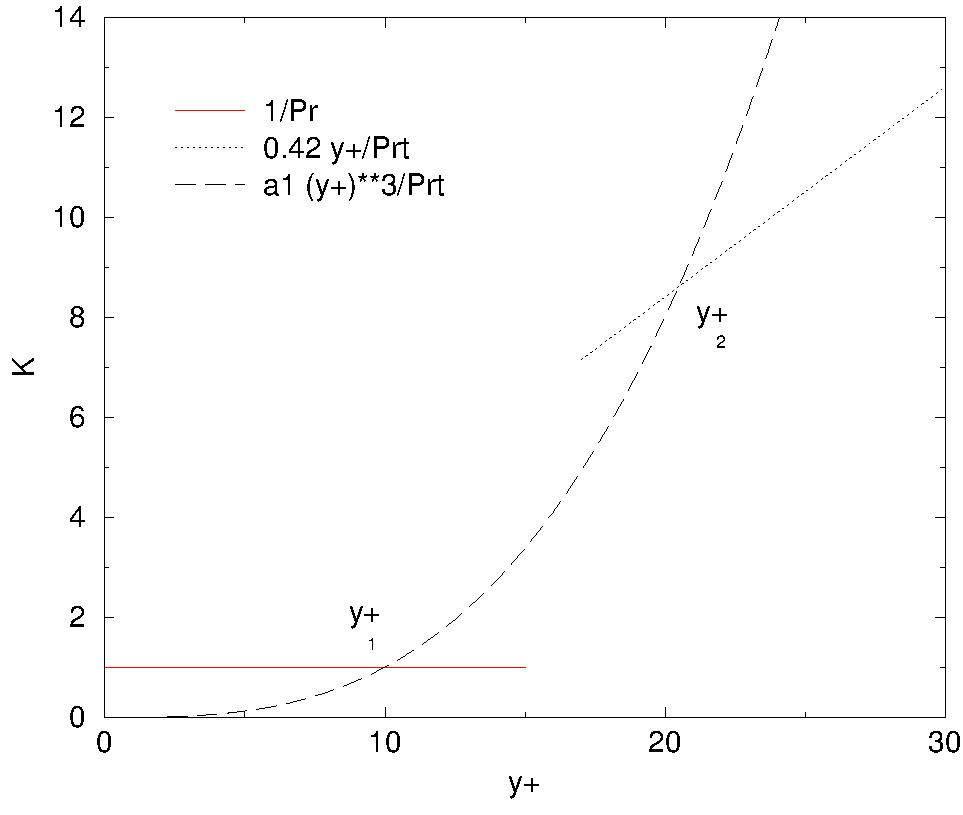
\includegraphics[height=8cm]{clthermique}}
\caption{$(a+a_t)/\nu$ as a function of $y^+$ obtained
                       for $\sigma=1$ and $\sigma_t=1$.}
\end{figure}


The values of $y^+_1$ and $y^+_2$ are obtained by calculating
the intersection points of the variations laws used
for $\mathcal{K}$.

The existence of an intermediate region depends upon the
values of $\sigma$.
Let's first consider the case where $\sigma$ cannot be neglected
compared to 1. In practise we consider  $\sigma > 0,1$
(this is the common case when scalar $f$ represents
the air or the water temperature in normal temperature
and pressure conditions). It is assumed that
$\displaystyle\frac{1}{\sigma}$ can be neglected compared to
$\displaystyle\frac{a_1 (y^+)^3}{\sigma_t}$ in the
intermediate region.
We thus obtain~:
\begin{equation}
  y^+_1 =\left(\displaystyle\frac{1000}{\sigma}\right)^\frac{1}{3} \qquad\qquad
  y^+_2 = \sqrt{\displaystyle\frac{1000\kappa}{\sigma_t}}
\end{equation}
The dimensionless equation~(\ref{Base_Clptur_Eq_Flux_scalaire_adim})
is integrated under the same hypothesis and we obtain the law of $f^+$~:
\begin{equation}
\left\{
\begin{array}{ll}
f^+ = \sigma \,y^+ & \text{if } y^+ < y^+_1 \\
f^+ = a_2 -\displaystyle\frac{\sigma_t}{2\,a_1\,(y^+)^2}& \text{if } y_1^+ \leqslant y^+ < y_2^+ \\
f^+ = \displaystyle\frac{\sigma_t}{\kappa}\,ln(y^+)+a_3& \text{if } y^+_2 \leqslant y^+\\
\end{array}
\right.
\end{equation}
where $a_2$ and $a_3$ are integration constants,
which have been chosen to obtain
a continuous  profile of $f^+$~:
\begin{equation}
a_2=15\sigma^{\frac{2}{3}}\qquad\qquad
a_3=15\sigma^{\frac{2}{3}}-\displaystyle\frac{\sigma_t}{2\kappa}
\left(1+
ln\left(\displaystyle\frac{1000\kappa}{\sigma_t}\right)\right)
\end{equation}

Let's now study the case where  $\sigma$ is much smaller than 1.
In practise it is assumed that $\sigma \leqslant 0,1$ (this is for
instance the case for liquid metals whose thermal conductivity is very
large, and who have Prandtl number of values of the order of 0.01).
The intermediate region then disappears and the coordinate of the
interface between the law used in the near-wall region and the one
used away from the wall is given by~:
\begin{equation}
y^+_0= \displaystyle\frac{\sigma_t}{\kappa\sigma}
\end{equation}

The dimensionless equation~(\ref{Base_Clptur_Eq_Flux_scalaire_adim})
is then integrated under the same hypothesis, and the law of
 $f^+$ is obtained~:
\begin{equation}
\left\{
\begin{array}{ll}
f^+ = \sigma \,y^+ & \text{if } y^+ \leqslant y^+_0 \\
f^+ = \displaystyle\frac{\sigma_t}{\kappa}\,
        ln\left(\displaystyle\frac{y^+}{y^+_0}\right)+\sigma \,y^+_0
                   & \text{if } y^+_0 < y^+\\
\end{array}
\right.
\end{equation}


\newpage
To summarize, the computation of $h_b$
\begin{equation}
h_b=\displaystyle\frac{\phi_b}{f_{b,ext}-f_{I'}}=\frac{\rho\,C\,u_k}{f^+_{I'}}
\end{equation}
is performed by calculating  $f^+_{I'}$ from $y^+=y^+_{I'}$
using the following laws.

If $\sigma\leqslant 0,1$, a two-layer model is used~:
\begin{equation}
\left\{
\begin{array}{ll}
f^+ = \sigma \,y^+ & \text{if } y^+ \leqslant y^+_0 \\
f^+ = \displaystyle\frac{\sigma_t}{\kappa}\,
        ln\left(\displaystyle\frac{y^+}{y^+_0}\right)+\sigma \,y^+_0
                   & \text{if } y^+_0 < y^+\\
\end{array}
\right.
\end{equation}
with
\begin{equation}
y^+_0= \displaystyle\frac{\sigma_t}{\kappa\sigma}
\end{equation}


If $\sigma > 0,1$, a three-layer model is used~:
\begin{equation}
\left\{
\begin{array}{ll}
f^+ = \sigma \,y^+ & \text{if } y^+ < y^+_1 \\
f^+ = a_2 -\displaystyle\frac{\sigma_t}{2\,a_1\,(y^+)^2}& \text{if } y_1^+ \leqslant y^+ < y_2^+ \\
f^+ = \displaystyle\frac{\sigma_t}{\kappa}\,ln(y^+)+a_3& \text{if } y^+_2 \leqslant y^+\\
\end{array}
\right.
\end{equation}
with
\begin{equation}
  y^+_1 =\left(\displaystyle\frac{1000}{\sigma}\right)^\frac{1}{3} \qquad\qquad
  y^+_2 = \sqrt{\displaystyle\frac{1000\kappa}{\sigma_t}}
\end{equation}
and
\begin{equation}
a_2=15\sigma^{\frac{2}{3}}\qquad\qquad
a_3=15\sigma^{\frac{2}{3}}-\displaystyle\frac{\sigma_t}{2\kappa}
\left(1+
ln\left(\displaystyle\frac{1000\kappa}{\sigma_t}\right)\right)
\end{equation}

%%%%%%%%%%%%%%%%%%%%%%%%%%%%%%%%%%
%%%%%%%%%%%%%%%%%%%%%%%%%%%%%%%%%%
\section*{Implementation}
%%%%%%%%%%%%%%%%%%%%%%%%%%%%%%%%%%
%%%%%%%%%%%%%%%%%%%%%%%%%%%%%%%%%%

%\etape{Mode de prescription des conditions aux limites\vspace{0,3cm}}
%%%%%%%%%%%%%%%%%%%%%%%%%%%%%%%%%%%%%%%%%%%%%%%%%%%%%%%%%%%%%%%%%%%%
This subroutines treats the variables \var{IVAR} on the faces \var{IFAC}
for which \var{ICODCL(IFAC,IVAR)}=5.

First the velocity of the wall (possibly zero) is projected onto
the plane parallel to the wall. Its three components in the
computation coordinate system are stored in the arrays
\\  \var{RCODCL(IFAC,IUIPH,1),RCODCL(IFAC,IVIPH,1)RCODCL(IFAC,IWIPH,1)}.

We then compute the local coordinate system  $\hat{\mathcal R}$.
For each face, it is stored in the vectors   $\vect{\tau}$ \var{(TX, TY, TZ)},
 $\vect{\tilde{n}}$ \var{(-RNX, -RNY,-RNZ)},
and $\vect{b}$ \var{(T2X, -T2Y,-T2Z)}.
It should be noticed that the third vector is only needed (and thus
only calculated) when the  $R_{ij}-\varepsilon$ model is used (for the
second order tensor projection). Additionally, if the norm of the tangential
velocity is lower than the arbitrary value \var{EPZERO}
($10^{-12}$), the indicator  \var{TXN0} is set to 0 (it is 0 otherwise)
and the vector  $\vect{\tau}$ is
\begin{itemize}
\item [-] chosen arbritrarily, in the plane orthogonal to $\vect{\tilde{n}}$ in
$R_{ij}-\varepsilon$  (the components of $\vect{\tilde{n}}$ are used
to construct  $\vect{\tau}$~; if  $\vect{\tilde{n}}$ is the zero vector,
 the code stops)~;
\item [-] zero, otherwise.
\end{itemize}

Once the local coordinate system has been calculated,
the subroutine \fort{clca66} is called with
\footnote{\var{CLSYME} = 0 indicates that we consider wall boundary conditions
and not symmetry boundary conditions. One is referred to \var{CLSYVT} for
more details on  \fort{clca66}.} \var{CLSYME} =0
(if the $R_{ij}-\varepsilon$  model is activated) in order to compute
the matrix \var{ALPHA}. The latter will be used to compute the values to
prescribe at the boundary, using the the values of the Reynolds stress
tensor at the points $I'$.

The friction velocities are then computed and stored in
\var{UET} ($=u^*$) and \var{UK} ($=u_k$). The subroutine \fort{cs\_wall\_functions.c}
 computes the friction velocity for the one velocity scale model
(\var{IDEUCH}=0). Fot the two velocity scale model (\var{IDEUCH}=1),
the (more simple) computation of \var{UET} and \var{UK} is performed
directly in  \fort{clptur}.

If one velocity scale model is activated, we impose \var{UK=UET} to
keep the coherence of the coding in the following of the subroutine.
However, if we are in the viscous sublayer, we force  \var{UK=0} to
obtain a zero value for $k$ and a zero flux for $\varepsilon$
(the value  \var{UET} is not used, because the condition of the velocity
is a no-slip condition and the Reynolds stresses are zero).

If we are in the viscous sublayer, we compute  \var{UET} again (and
\var{YPLUS} if we use the one velocity scale model) since the previous
derivation has been made under the assumption that we were in the
logarithmic region.


The boundary conditions for the velocity are then completed.
\begin{itemize}

\item [-] In $k-\varepsilon$, the coefficients $A_{flux}$
(coming from the analysis of the tangential velocity) for the three
components of the velocity are stored in
 $$\var{COEFA(IFAC,ICLUF)}, \var{COEFA(IFAC,ICLVF)} \,\text{ et
}\,\var{COEFA(IFAC,ICLWF)}$$, respectively.\\
 Similarly, the coefficients $B_{flux}$ are stored in
$$\var{COEFB(IFAC,ICLUF)}, \var{COEFB(IFAC,ICLVF)} \,\text{ et
}\,\var{COEFB(IFAC,ICLWF)}.$$ The boundary conditions
coming from the analysis of the velocity gradient $A_{grad}$ and
$B_{grad}$ are stored in  $$\var{COEFA(IFAC,ICLU)},
\var{COEFA(IFAC,ICLV)}, \var{COEFA(IFAC,ICLW)}$$ and
$$\var{COEFB(IFAC,ICLU)}, \var{COEFB(IFAC,ICLV)}, \var{COEFB(IFAC,ICLW)}.$$

\item [-] When the tangential velocity at $I'$ is lower than
\var{EPZERO}, the indicator \var{TXN0} is set to zero (otherwise,
\var{TXN0} is 1).
Likewise,  when the value of
$y^+$ is lower or equal to $10,88$, the indicator
\var{UNTURB} is set to 0 (otherwise, it is 1). Both these indicators
are used to set to zero the coefficients $A$, and thus to prescribe no-slip
boundary conditions.

\item [-] the velocity of the wall is taken into account in the
boundary conditions (coefficients \var{COEFA}).

\end{itemize}

The conditions of the turbulent variables are then filled in.
Additional details are provided for the Reynolds tensor
in  $R_{ij}-\varepsilon$.
Using tensorial notation, we want to obtain
$\tens{R}_F = E_{loglo}\,\hat{\tens{R}}_F\,E^t_{loglo}$, where
$\hat{\tens{R}}_F$ is the stress tensor to impose in the local
coordinate system and $E_{loglo}$ is the transformation matrix.
The tensor in the local coordinate system is defined by the boundary
conditions detailed above,  $\hat{\tens{R}}_F=\hat{\tens{R}}^{B=1}_F$,
with \footnote{The parameter
$B$ permits to set to zero two terms if needed.}~:
\begin{equation}
\hat{\tens{R}}^B_{F}=\left[\begin{array}{lll}
\hat{R}_{\tau\tau,I'}&-Bu^*u_k                       &0\\
-Bu^*u_k             &\hat{R}_{\tilde{n}\tilde{n},I'}&0\\
0                    &0                              &\hat{R}_{bb,I'}
\end{array}\right]
\end{equation}

The Reynolds tensor is stored in a vector with 6 components (at points $I'$
of the boundary faces, these values are stored in \var{RIJIPB(IFAC,II)},
with \var{IFAC} the index of the face and \var{II} the index of the stress,
from 1 to 6 \var{II} refers to $R_{11},R_{22}, R_{33}$,
$R_{12}, R_{13}$ and $R_{23}$, respectively. The array \var{IFAC} of
dimension $6\times 6$ (calculated by \fort{clca66}) is used to perform
the necessary change of coordinate system computations, and to obtain
the values of $\hat{\tens{R}}^{B=0}_F$ from the values stored in
\var{RIJIPB(IFAC,II)}.
Thus,
\begin{itemize}
\item[-] for each Reynolds stress \var{ISOU},
in case of explicit boundary conditions (\var{ICLPTR}=0), we set
\var{COEFA(IFAC,ISOU)}  to the corresponding value of
$\tens{R}^{B=1}_F$ obtained by first computing
$\tens{R}^{B=0}_F$ by
$\sum_{II=1,6}$\var{ALPHA(ISOU,II)*RIJIPB(IFAC,II)}, and then by adding
the quantity factorised by B in the previous sum, in order to obtain
the complete value of $\tens{R}^{B=1}_F$. Since the boundary conditions
are explicit,  \var{COEFB} is set to  0.
\item[-] in case of semi-implicit boundary conditions (\var{ICLPTR}=1),
for each Reynolds stress \var{ISOU},
we store in the array \var{COEFA(IFAC,ISOU)} the corresponding value
$\tens{R}^{B=1}_F$  minus the terms which depend upon
\var{RIJIPB(IFAC,ISOU)} (which will be implicited)
This value is obtained by first calculating \\
$\sum_{II=1,6|II\neq ISOU}$\var{ALPHA(ISOU,II)*RIJIPB(IFAC,II)},
and then by adding the quantity  factorised by B in order to obtain
the value of $\tens{R}^{B=1}_F$ minus the term \\
\var{ALPHA(ISOU,ISOU) RIJIPB(IFAC,ISOU)}.
\var{ALPHA(ISOU,ISOU)} is then stored in \var{COEFB} (implicit part of
the boundary conditions)\footnote{the implicit part does not include
the tangential stress due to the friction velocities and thus the boundary
conditions are not fully implicit.}.
\end{itemize}

The boundary conditions of the scalars are then completed. The coefficients
\var{COEFA} and \var{COEFB} are simply calculated using the boundary
conditions previously described. The only difficulty consists in dealing
adequatly with the various values necessary to compute the exchange
coefficient $h_b$ without any mistake.


The indicator \var{ISCSTH} gives for each {\it VarScalaires} the value
of  $C$ to use in the treatment of the boundary conditions.
Thus, for \var{ISCSTH}=1,
the variable should be treated as a temp\'erature, with $C=C_p$. For
\var{ISCSTH}=0 or 2, the variable should be treated as a passive scalar
or as an enthalpy, respectively, with  $C=1$ (dimensionless constant)
in both cases. For \var{ISCSTH}=3, the variables is the resolved energy
in the framework of the compressible module  (see \fort{cfxtcl}). We then
have $C=1$.

Additionally, a strictly positive value of the integer \var{IPCCP}
indicates that $C_p$ varies in space and that it is available in the
array \var{PROPCE(IEL,IPCCP )} (filled in \var{USPHYV}). When \var{IPCCP}
is zero, $C_p$ is constant and it is available
as a real number \var{CP0}.


The indicator \var{IHCP} gathers these informations~:
\begin{itemize}
\item [-] \var{IHCP} = 0 : \var{CPP} = $C=1$
\item [-] \var{IHCP} = 1 : \var{CPP} = $C=C_p$ uniform in space
\item [-] \var{IHCP} = 2 : \var{CPP} = $C=C_p$ variable in space
\end{itemize}

For {\it VarScalaire} \var{LL}, the indicator \var{IVISLS(LL)}
indicates if $\displaystyle\frac{\alpha_m}{C}$
is variable in space and available in
the array \var{PROPCE(IEL,IPCVSL)}
(\var{IVISLS} $> 0$) or if is uniform in space and available
as a real number
\var{VISLS0(LL)} (\var{IVISLS} $= 0$). We take \var{RKL}$ =
\displaystyle\frac{\alpha_m}{C}$.

The local Prandtl number is then calculated as \var{PRDTL} $ =
\displaystyle\frac{\mu}{\alpha_m/C}$ ($\mu$ is the molecular dynamic viscosity
available in \var{VISCLC}).

The coefficient $h_{int}=\displaystyle\frac{\alpha}{\overline{I'F}}$  is
then calculated and stored in \var{HINT}.

When a turbulence model is activated,
the subroutine \var{HTURBP} computes \var{HFLUI} $ =
Pr\displaystyle\frac{y^+}{T^+}$ (or \var{HFLUI}~$ = 1$
in the viscous sublayer),
which is then immediately multiplied by \var{CPP*RKL/DISTBF}$ =
\displaystyle\frac{\alpha_m}{\overline{I'F}}$ to obtain \var{HFLUI} $ = h_b =
\displaystyle\frac{\rho C u_k}{T^+}$ (or \var{HFLUI} $ = h_b = \displaystyle\frac{\alpha_m}{\overline{I'F}}$ in the viscous sublayer).
If the calculation is performed in laminar, we simply have
 \var{HFLUI} = \var{HINT} ($ = h_b = h_{int}=\displaystyle\frac{\alpha}{\overline{I'F}}$)

In case we wish to store the exchange coefficient (coupling with SYRTHES),
\var{HFLUI} is kept in the array \var{HBORD}. In case the raditation module
is used, \var{HFLUI} is stored in the work array \var{RA(IHCONV)}.

We then have all the information necessary to compute the coefficients
$A$ and $B$  (\var{COEFA} and \var{COEFB}) relative to the treated variable.
Finally one can give the following correspondances
to relate the source code implementation to
expression (\ref{Base_Clptur_eq_fbint_clptur})~:
\var{HEXT} $ = h_{imp,ext}$, \var{PIMP} $ = f_{imp,ext}$,
\var{HREDUI} $ = h_r$, \var{HINT} $ = h_{int}$,  \var{HFLUI} $ = h_b$.




\newpage
%%%%%%%%%%%%%%%%%%%%%%%%%%%%%%%%%%
%%%%%%%%%%%%%%%%%%%%%%%%%%%%%%%%%%
\section*{Points to treat}
%%%%%%%%%%%%%%%%%%%%%%%%%%%%%%%%%%
%%%%%%%%%%%%%%%%%%%%%%%%%%%%%%%%%%


The use of \var{HFLUI/CPP} when \var{ISCSTH} is 2 (case with
radiation) needs to be checked (\var{CPP} is actually 1 in this case).

The boundary conditions of the velocity are based on derivations
focusing on only one term of the tangential stress
$(\mu_I+\mu_{t,I})(\ggrad{\vect{u}})\,\vect{n}$ without taking
into account the tranpose gradient.

In order to establish the boundary conditions of the velocity in
$k-\varepsilon$ based on the constraint , a projection onto the plane
tangent to the wall and an arbitrary zero normal velocity
are introduced.

The hypothesis made in order to establish formulae for the different types
of boundary conditions (dissipation, velocities) are based on the assumption
that the mesh is orthogonal at the wall. This assumption is extended
without any caution to the case of non-orthogonal meshes.

The one velocity scale (\fort{cs\_wall\_functions.c}) wall function requires
solving an equation using a Newton algorithm.
The computational cost of the latter is low. One can also used
a  $1/7$ power law (Werner et Wengle) which yields results which are as
accurate as the logarithmic law in the logarithmic region, and which permits
analytical resolutions (chosen option in LES mode). Be careful however,
since with this law, the intersection with the linear law is
slightly different, which thus requires some adaptations (intersection
around 11.81 instead of 10.88 for the law adopted here
$U^+=8,3\,(y^+)^\frac{1}{7}$).


The values of all the physical properties are taken at the cell centres,
without any reconstruction. Without modifying this approach, it would be
useful to keep this in mind.

%
%
%
%Pb de continuite si YPLULI.NE.10.88
%
% Le mode de r\'esolution permettant d'obtenir $u^*$ est particulier. Avec le
%mod\`ele \`a une \'echelle de vitesse, on \'evalue
%tout d'abord la vitesse de frottement $u^*$ issue de la loi logarithmique. On
%pose $u_k=u^*$, puis on calcule la valeur de $y^+$.  Avec le
%mod\`ele \`a deux \'echelles, on calcule tout d'abord $u_k$, on en d\'eduit
%$y^+$ puis $u^*$. Dans les deux cas, si
%$y^+\leqslant y^+_{lim}=\displaystyle\frac{2}{\kappa}$, on applique une condition
%d'adh\'erence (vitesse impos\'ee nulle \`a la paroi, \'energie turbulente et
%tensions de Reynolds impos\'ees nulles, flux nul pour la dissipation).
%Il serait bon de v\'erifier que cette m\'ethode, qui utilise une loi
%logarithmique jusqu'\`a de tr\`es petites
%valeurs de $y^+$, ne conduit pas \`a des valeurs trop faibles de la
%vitesse de frottement lorsqu'on s'approche de la paroi ($y^+ \leqslant 10$).
%La figure \ref{Base_Clptur_fig_loi_log_clptur} propose une illustration~: supposons qu'en un
%point on obtienne, avec la m\'ethode actuelle, $u+\approx 8,6$ et
%$y^+\approx 4,3$. On en d\'eduit alors que la vitesse de frottement est
%$u^*\approx 1$ (courbe logarithmique en trait plein (noire) repr\'esentant
%$ln(y^+)/0,42+5,2$).
%Toutes choses \'egales par ailleurs (ce qui constitue une
%hypoth\`ese en soi), avec une m\'ethode prenant en compte une loi lin\'eaire en
%dessous de $y^+\approx 10$, on aurait obtenu $u^*\approx 2$
%(courbe lin\'eaire en trait plein (rouge) repr\'esentant $2y^+$). Bien
%entendu, cette analyse est relativement na\"\i ve et ne prend pas en compte le
%caract\`ere implicite des r\'esolutions ainsi que le fait qu'il est d'ordinaire
%peu recommand\'e de placer la premi\`ere maille \`a des valeurs aussi faibles de
%$y^+$ avec les mod\`eles de type haut Reynolds.
%
%\begin{figure}[h]
%\centerline{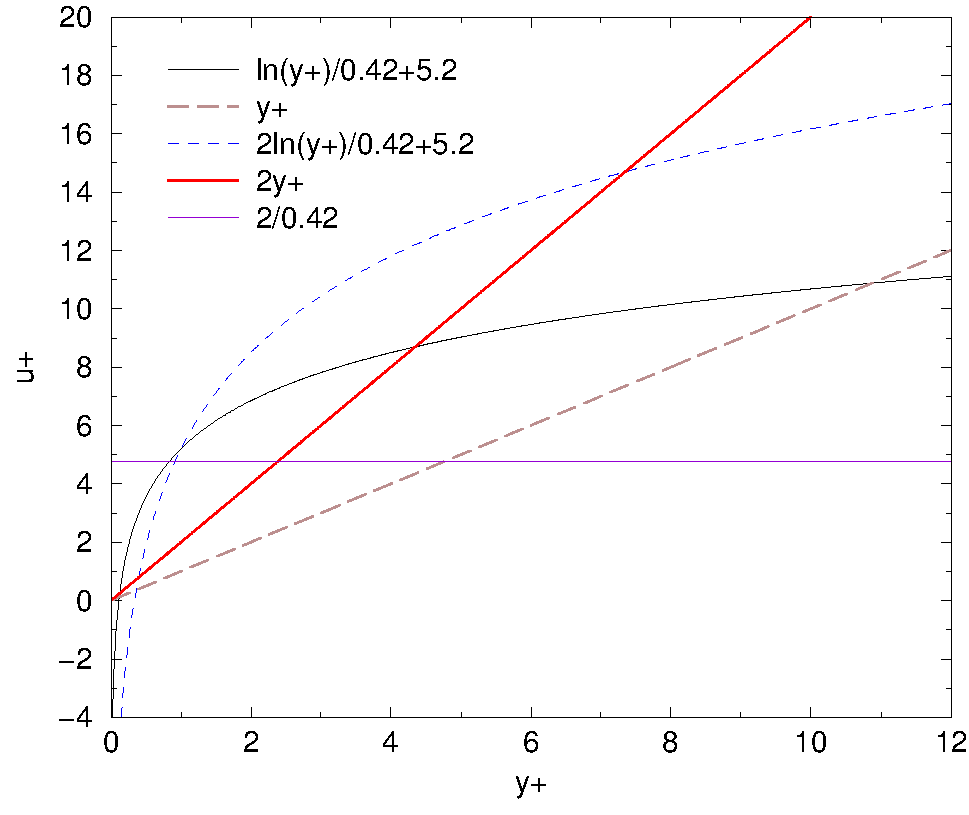
\includegraphics[height=7cm]{loilog}}
%\caption{\label{Base_Clptur_fig_loi_log_clptur}D\'etermination de $y^+$.}
%\end{figure}



% Plus d'actualite a priori, mais pistes de reflexion quand meme
%La limitation par valeur minimale de la vitesse dans (\ref{Base_Clptur_eq_ugrad_clptur})
%a \'et\'e corrig\'ee dans la version 1.1.0.q.
%Auparavant, la formulation \'etait susceptible de conduire
%\`a une valeur trop faible du gradient de vitesse et donc de la production
%turbulente en paroi. Elle s'\'ecrivait~:
%\begin{equation}
%u_{\tau,F,grad} =u_{\tau,I'}-\displaystyle\frac{u^*}{\kappa}min\left[max\left(1,
%2\sqrt{\displaystyle\frac{\rho_I\kappa\, u_k I'F}{\mu_{t,I}}
%}-\displaystyle\frac{1}{2}\right),ln\frac{2}{\kappa}+5,2\kappa\right]
%\end{equation}
%La  formulation a \'et\'e modifi\'ee~:
%\begin{equation}\notag
%u_{\tau,F,grad} =max\left(u^*(\frac{1}{\kappa}ln\displaystyle\frac{2}{\kappa}+5,2),
%u_{\tau,I'}-\displaystyle\frac{u^*}{\kappa}\left[max\left(1,
%2\sqrt{\displaystyle\frac{\rho_I\kappa\, u_k I'F}{\mu_{t,I}}
%}-\displaystyle\frac{1}{2}\right)\right]\right)
%\end{equation}
%Elle a \'et\'e adopt\'ee apr\`es des tests sur des
%configurations de validation (canal, marche descendante,  jet impactant, dune,
%echo, rra) qui n'ont montr\'e aucune influence de la modification.
%\`A partir de la version 1.1.0.t, on a utilis\'e la valeur
%$y^+_\text{lim}=10,88$ et non plus $\frac{2}{\kappa}$ pour caract\'eriser le
%passage de la loi lin\'eaire \`a la loi logarithmique et la
%relation a donc \'et\'e modifi\'ee comme suit~:
%\begin{equation}\notag
%u_{\tau,F,grad} =max\left(u^*(\frac{1}{\kappa}ln(y^+_\text{lim})+5,2),
%u_{\tau,I'}-\displaystyle\frac{u^*}{\kappa}\left[max\left(1,
%2\sqrt{\displaystyle\frac{\rho_I\kappa\, u_k I'F}{\mu_{t,I}}
%}-\displaystyle\frac{1}{2}\right)\right]\right)
%\end{equation}
%Comme, pour des $y^+$ inf\'erieurs \`a $y^+_\text{lim}$, on applique une
%condition d'adh\'erence, cette approche n'est pas continue au voisinage de
%$y^+_\text{lim}$. Il serait utile de se pencher sur la question.
%Il faut cependant garder \`a l'esprit que la condition
%de Dirichlet pour $k$ est prise nulle quand  $y^+$ est inf\'erieur \`a
%$y^+_\text{lim}$, ce qui tend \'egalement  \`a annuler la production,
%quelle que soit la condition \`a la limite utilis\'ee pour la vitesse.


For the thermal law with very small Prandtl numbers compared to 1,
Arpaci and Larsen suggest $y_0^+ \simeq 5/Pr$ (with proof from
experimental data) rather than $Pr_t/(Pr\,\kappa)$  (current value,
computed as the analytical intersection of the linear and logarithmic
laws considered). One should address this question.



%-----------------------------------------------------------------------
%
%     This file is part of the Code_Saturne Kernel, element of the
%     Code_Saturne CFD tool.
%
%     Copyright (C) 1998-2008 EDF S.A., France
%
%     contact: saturne-support@edf.fr
%
%     The Code_Saturne Kernel is free software; you can redistribute it
%     and/or modify it under the terms of the GNU General Public License
%     as published by the Free Software Foundation; either version 2 of
%     the License, or (at your option) any later version.
%
%     The Code_Saturne Kernel is distributed in the hope that it will be
%     useful, but WITHOUT ANY WARRANTY; without even the implied warranty
%     of MERCHANTABILITY or FITNESS FOR A PARTICULAR PURPOSE.  See the
%     GNU General Public License for more details.
%
%     You should have received a copy of the GNU General Public License
%     along with the Code_Saturne Kernel; if not, write to the
%     Free Software Foundation, Inc.,
%     51 Franklin St, Fifth Floor,
%     Boston, MA  02110-1301  USA
%
%-----------------------------------------------------------------------
%


\programme{clptrg}


\vspace{1cm}
%%%%%%%%%%%%%%%%%%%%%%%%%%%%%%%%%%
%%%%%%%%%%%%%%%%%%%%%%%%%%%%%%%%%%
\section{Fonction}
%%%%%%%%%%%%%%%%%%%%%%%%%%%%%%%%%%
%%%%%%%%%%%%%%%%%%%%%%%%%%%%%%%%%%
Ce sous-programme est d�di� au calcul des conditions aux limites en paroi
rugueuse. On utilise le
formalisme introduit dans \var{CONDLI} pour les conditions 
aux limites g\'en\'erales. 

Par conditions aux limites en paroi, on entend ici l'ensemble des conditions aux
limites pour la vitesse, les grandeurs turbulentes ($k$, $\varepsilon$),
la temp\'erature lorsqu'elle a une valeur de paroi impos\'ee   
(ou l'enthalpie et plus g\'en\'eralement les 
{\it VarScalaires}\footnote{Comme dans \fort{condli}, on d\'esignera ici par 
{\it VarScalaire} toute variable solution
d'une \'equation de convection-diffusion autre que la 
vitesse, la pression et les grandeurs turbulentes $k$, $\varepsilon$. La
d\'enomination {\it VarScalaire} pourra en particulier se rapporter 
\`a la temp\'erature, \`a l'enthalpie ou \`a un scalaire passif.} 
\`a traiter en paroi en prenant en compte une loi de similitude
pour la couche limite associ\'ee). Pour les {\it VarScalaires}, en particulier,
lorsque les conditions aux limites de paroi sont du type Neumann (homog\`ene ou non),
elles sont trait\'ees dans \fort{condli} et on ne s'y int\'eresse donc pas
ici. En particulier, les conditions aux limites des  {\it VarScalaires}
repr\'esentant la variance de fluctuations d'autres  {\it VarScalaires} ne
sont pas trait\'ees ici car leur traitement en paroi est de type Neumann homog\`ene. 

On indique comment sont calcul\'es les couples de coefficients 
$A_b$ et $B_b$ qui sont utilis\'es pour le calcul de certains 
termes discrets des \'equations \`a r\'esoudre et qui
permettent  en particulier de d\'eterminer une valeur associ\'ee aux faces 
de bord $f_{b,int}$ (en un point localis\'e au ``centre'' de la face de bord, 
barycentre de ses sommets) par la
relation $f_{b,int} = A_b+B_b\,f_{I'}$ ($f_{I'}$ est la valeur de 
la variable au point
$I'$, projet\'e du centre de la cellule jouxtant le bord sur la droite 
normale \`a 
la face de bord et passant par son centre~: voir la figure~\ref{fig_flux_clptur}). 

\begin{figure}[h]
\centerline{\includegraphics[height=7cm]{\repgraphics/fluxbord}}
\caption{\label{fig_flux_clptur}Cellule de bord.}
\end{figure}

%%%%%%%%%%%%%%%%%%%%%%%%%%%%%%%%%%
%%%%%%%%%%%%%%%%%%%%%%%%%%%%%%%%%%
\section{Discr\'etisation}
%%%%%%%%%%%%%%%%%%%%%%%%%%%%%%%%%%
%%%%%%%%%%%%%%%%%%%%%%%%%%%%%%%%%%

\etape{Notations\vspace{0,3cm}}
%%%%%%%%%%%%%%%%%%%%%%%%%%%%%%%%%%%%%%%%%%%%%%%%%%%%%%%%%%%%%%%%%%%%%%%%%%%%%%%
La vitesse de la paroi est not\'ee
$\vect{v}_p$. On la suppose projet\'ee dans le plan tangent \`a la paroi (si
elle ne l'est pas, le code la projette).

La vitesse du fluide est not\'ee $\vect{u}$. L'indice $I$, $I'$ ou $F$ d\'esigne le
point auquel elle est estim\'ee. La composante tangentielle par rapport \`a la
paroi est not\'ee $u_\tau$. 
 La vitesse du fluide dans le rep\`ere li\'e \`a la paroi (vitesse
``relative'') est not\'ee $\vect{u}^r=\vect{u} - \vect{v}_p$. 

Le rep\`ere orthonorm\'e li\'e \`a la paroi est not\'e 
$\hat {\mathcal R}=(\vect{\tau},\vect{\tilde{n}},\vect{b})$. 
\begin{itemize}
\item [$\bullet$] $\vect{\tilde{n}}=-\vect{n}$ est le vecteur norm\'e
orthogonal \`a la paroi et dirig\'e vers l'int\'erieur du domaine de calcul.
\item [$\bullet$] $\vect{\tau} = \displaystyle\frac{1}{\|\vect{u}^r_{I'}-(\vect{u}^r_{I'}\,.\,\vect{\tilde{n}})\|}\left[\vect{u}^r_{I'}-(\vect{u}^r_{I'}\,.\,\vect{\tilde{n}})\right]$ est le vecteur norm\'e port\'e par la projection de la vitesse 
relative en $I'$, $\vect{u}^r_{I'}$, dans le plan tangent \`a la
paroi ({\it i.e.} orthogonal \`a $\vect{\tilde{n}}$)~: voir la
figure~\ref{fig_flux_clptur}. 
\item [$\bullet$] $\vect{b}$ est le vecteur norm\'e compl\'etant le rep\`ere direct. 
\end{itemize}

\vspace{0.5cm}

Dans le cas du {\bf mod\`ele \`a deux  \'echelles de vitesse}, on note~:
\begin{itemize}
\item [-] $u_k$ la
vitesse de frottement en paroi obtenue \`a partir de l'\'energie turbulente.

\item [-] $u^*$ la vitesse de frottement en paroi d\'etermin\'ee \`a
partir de la relation $ \displaystyle\frac{u^r_{\tau,I'}}{u^*} = f(z_p)$. 

\item [-] $z_p$  repr�sente une distance � la paroi
      (c'est � dire la distance depuis le bord du domaine de calcul),  soit 
$z_p= I'F$ (voir la figure~\ref{fig_flux_clptur}). La fonction $f$ traduit la forme id�ale du profil de
      vitesse. Dans l'atmosph�re, cette fonction est donn�e par
      une loi de type logarithmique faisant intervenir la rugosit� dynamique de
      la paroi $z_0$~:

$f(z_p)= \displaystyle\frac{1}{\kappa} ln \left ( \displaystyle \frac
      {z_p+z_0}{z_0} \right ) $


\item [-] Les deux \'echelles de vitesse $u_k$ et $u^*$ sont simples \`a
      calculer mais leur obtention  
n\'ecessite la connaissance de l'\'energie turbulente $k_I$ au centre de la
maille jouxtant la face de bord. 

\item [-] Le mod\`ele \`a deux \'echelles 
est le mod\`ele par d\'efaut dans \CS. Il permet souvent, et en particulier 
dans les cas avec transfert thermique, de diminuer les effets de certains 
d\'efaut li\'es au mod\`ele $k-\varepsilon$ (exemple classique du jet impactant).  
\end{itemize}

On se sert plus bas de $u^*$ et $u_k$ pour les conditions aux limites portant
sur la vitesse et les scalaires (temp\'erature en particulier). 


\begin{equation}
\label{Eq_Mod_'2ech_Vit}
\begin{array}{l}
\text{\bf Mod\`ele \`a deux \'echelles de vitesse}\\
\left\{\begin{array}{l}
u_k = C_\mu^\frac{1}{4}k_I^\frac{1}{2}\\
u^* \text{solution de }  \displaystyle\frac{u^r_{\tau,I'}}{u^*} =
\displaystyle\frac{1}{\kappa}ln(z_k)\\
z_k=\displaystyle\frac{I'F+z_0}{z_0} = \displaystyle\frac{z_p+z_0}{z_0}\\
\text{   avec   } C_\mu =0,09 \text{  et }  \kappa = 0,42 
\end{array}\right.\\ 
\end{array}
\end{equation}


\vspace{0.5cm}

Dans le cas du {\bf mod\`ele \`a une \'echelle de vitesse}, on note $u^*$ l'unique vitesse
de frottement en paroi solution de l'\'equation 
$\displaystyle\frac{u^r_{\tau,I'}}{u^*} = f(z_p)$. La grandeur
$z_p$  repr\'esente une distance \`a la paroi, soit
$z_p=I'F$. La fonction $f$ traduit la forme id\'eale du profil de vitesse comme
pour le mod\`ele \`a deux \'echelles de vitesses. On peut 
noter que cette vitesse de frottement, d'un calcul plus d\'elicat (point fixe), 
s'obtient  cependant sans faire r\'ef\'erence aux
variables turbulentes ($k$, $\varepsilon$). Par commodit\'e, on posera
dans le cas du mod\`ele \`a une \'echelle $u_k=u^*$.

On se sert plus bas de $u^*$ et $u_k$ pour les conditions aux limites portant
sur la vitesse et les scalaires (temp\'erature en particulier). 

\begin{equation}
\begin{array}{l}
\text{\bf Mod\`ele \`a une \'echelle de vitesse}\\
\left\{\begin{array}{l}
u_k = u^*\\
u^* \text{solution de }  \displaystyle\frac{u^r_{\tau,I'}}{u^*} =
\displaystyle\frac{1}{\kappa}ln(z_k)\\
z_k=\displaystyle\frac{I'F+z_0}{z_0} = \displaystyle\frac{z_p+z_0}{z_0}\\
\text{   avec   } C_\mu =0,09 \text{  et }  \kappa = 0,42 
\end{array}\right.\\ 
\end{array}
\end{equation}

\etape{Conditions aux limites pour la vitesse en $k-\varepsilon$\vspace{0,3cm}}
%%%%%%%%%%%%%%%%%%%%%%%%%%%%%%%%%%%%%%%%%%%%%%%%%%%%%%%%%%%%%%%%%%%%%%%%%%%%%%%
On consid\`ere tout d'abord les conditions utilis\'ees dans le cas d'un calcul
r\'ealis\'e avec le mod\`ele $k-\varepsilon$. Ce sont en effet les plus
complexes et les plus g\'en\'erales. 

Les conditions aux limites sont n�cessaires pour imposer au bord la contrainte
tangentielle $\sigma_\tau=\rho_Iu^*u_k$ ad�quate dans l'\'equation de  quantit\'e de
mouvement\footnote{Proposition de modification des conditions aux limites de
paroi turbulente pour le Solveur Commun dans le cadre du mod\`ele
$k-\varepsilon$ standard, rapport EDF HI-81/00/019/A, 2000, M. Boucker, J.-D. Mattei.} 
($\rho_I$ est la masse volumique au centre de la
cellule $I$). Le terme qui n\'ecessite des conditions aux limites est celui qui contient la
d\'eriv\'ee de la vitesse dans la direction normale \`a la paroi, 
soit\footnote{Le terme en gradient transpos\'e est trait\'e dans \fort{vissec} 
et ne sera pas consid\'er\'e ici.}~:
$(\mu_I+\mu_{t,I})\ggrad{\vect{u}}\,\vect{n}$. Il appara\^\i t au second membre
de l'\'equation de quantit\'e de mouvement usuelle (voir \fort{bilsc2} et \fort{preduv}). 

Dans le cas o\`u le mod\`ele $k-\varepsilon$ a tendance \`a surestimer la
production de l'\'energie turbulente, l'\'echelle de longueur du mod\`ele,
$L_{k-\varepsilon}$, 
peut devenir significativement plus grande que l'\'echelle th\'eorique maximale
des tourbillons de la couche limite turbulente $L_{\text{th\'eo}}$. On note : 
\begin{equation}
\left\{\begin{array}{l}
L_{k-\varepsilon} = C_{\mu}\displaystyle\frac{k^\frac{3}{2}}{\varepsilon}\\
L_{\text{th\'eo}} = \kappa\, \left( I'F+z_0 \right) = \kappa\, \left(z_p+z_0 \right)
\end{array}\right.
\end{equation}

Dans le cas o\`u $L_{k-\varepsilon}>L_{\text{th\'eo}}$, on a donc
$\mu_{t,I}>\mu_{t}^{lm}$ avec $\mu_{t,I}$ la viscosit\'e turbulente du mod\`ele
$k-\varepsilon$ au point $I$ et $\mu_{t}^{lm}=\rho_I L_{\text{th\'eo}}u_k$ la
viscosit\'e turbulente du mod\`ele de longueur de m\'elange. En outre, la
contrainte tangentielle peut s'\'ecrire en faisant appara\^\i tre la viscosit\'e
turbulente, soit~: 
\begin{equation}
\sigma_\tau = \rho_Iu^*u_k = \displaystyle\frac{u^*}{\kappa\,
 \left(I'F+z_0 \right)}
\underbrace{\rho_I\kappa\, \left( I'F+z_0 \right)  u_k}_{\mu^{lm}_t}
\end{equation}
L'\'echelle de viscosit\'e introduite dans la contrainte est alors en
contradiction avec celle d\'eduite de la turbulence calcul\'ee alentour par le
mod\`ele. On pr\'ef\`ere d\`es lors \'ecrire, en utilisant l'\'echelle de
longueur du $k-\varepsilon$ chaque fois qu'elle est inf\'erieure \`a la limite
$L_{\text{th\'eo}}$~: 
\begin{equation}
\sigma_\tau = \displaystyle\frac{u^*}{\kappa\, \left(I'F+z_0 \right)} max(\mu_{t}^{lm},\mu_{t,I})
\end{equation}

On peut alors utiliser cette valeur  pour le calcul du flux
diffusif qui en d\'epend dans l'\'equation de Navier-Stokes~: 
\begin{equation}\label{eq_grad_sigma_clptur}
(\mu_I+\mu_{t,I})\ggrad{\vect{u}}\,\vect{n}=-\sigma_\tau \vect{\tau}
\end{equation} 

Or, le gradient de vitesse (gradient \`a la face de bord) est calcul\'e dans le
code sous la forme suivante~: 
\begin{equation}\label{eq_grad_uf_clptur}
(\mu_I+\mu_{t,I})\ggrad{\vect{u}}\,\vect{n}=
\displaystyle\frac{(\mu_I+\mu_{t,I})}{\overline{I'F}}(\vect{u}_F-\vect{u}_{I'})
\end{equation} 

Du rapprochement de (\ref{eq_grad_sigma_clptur}) et de
(\ref{eq_grad_uf_clptur}) on tire alors la valeur de $\vect{u}_F$ \`a
imposer, soit $\vect{u}_{F,flux}$~(respect du flux de quantit\'e de mouvement)~:
\begin{equation}\label{eq_uf_flux_clptur}
\begin{array}{ll}
\vect{u}_{F,flux}&=\vect{u}_{I'}-\displaystyle\frac{\overline{I'F}}{\mu_I+\mu_{t,I}}\sigma_\tau \vect{\tau}\\
                 &=\vect{u}_{I'}-\displaystyle\frac{u^*}{\kappa\,
		  (\mu_I+\mu_{t,I})} max(\mu_{t}^{lm},\mu_{t,I})
		  \, \displaystyle\frac {I'F} {\left(I'F+z_0 \right)} \vect{\tau}
\end{array} 
\end{equation} 

En r\'ealit\'e, une approximation suppl\'ementaire est r\'ealis\'ee, qui
consiste \`a imposer la vitesse normale nulle \`a la paroi et \`a utiliser
l'\'equation (\ref{eq_uf_flux_clptur}) projet\'ee sur le plan tangent \`a la
paroi, soit~:
\begin{equation}
\vect{u}_{F,flux}=\left[u_{\tau,I'}-\displaystyle\frac{u^*}{\kappa\,
(\mu_I+\mu_{t,I})} max(\mu_{t}^{lm},\mu_{t,I}) \, \displaystyle\frac {I'F} {\left(I'F+z_0 \right)} \right]\vect{\tau}
\end{equation} 

Enfin, on peut \'egalement faire appara\^\i tre la vitesse de la paroi
dans l'expression finale~:
\begin{equation}
\begin{array}{l}
\text{\bf Conditions aux limites sur la vitesse de type ``flux''}\,(k-\varepsilon)\\
\left\{\begin{array}{l}
\vect{u}_{F,flux}=\vect{v}_p+\left[u^r_{\tau,I'}-\displaystyle\frac{u^*}{\kappa\,
(\mu_I+\mu_{t,I})} max(\mu_{t}^{lm},\mu_{t,I})  \, \displaystyle\frac {I'F} {\left(I'F+z_0 \right)}\right]\vect{\tau}
\end{array}\right.\\ 
\end{array} 
\end{equation} 

Un premier couple de coefficients $A_{flux}$ et $B_{flux}$ s'en d\'eduit (pour
chaque composante de vitesse s\'epar\'ement) et il n'est utilis\'e que pour le
calcul du terme d\'ependant de la contrainte tangentielle (voir \fort{bilsc2})~: 
\begin{equation}
\begin{array}{l}
\text{\bf Coefficients associ\'es aux conditions aux limites sur la vitesse de
type ``flux''} (k-\varepsilon)\\
\left\{\begin{array}{l}
\vect{A}_{flux}=\vect{v}_p+\left[u^r_{\tau,I'}-\displaystyle\frac{u^*}{\kappa\,
(\mu_I+\mu_{t,I})} max(\mu_{t}^{lm},\mu_{t,I}) \, \displaystyle\frac {I'F} {\left(I'F+z_0 \right)} \right]\vect{\tau} \\
\vect{B}_{flux} = \vect{0}
\end{array}\right.
\end{array}
\end{equation} 

On a vu ci-dessus comment imposer une condition \`a la limite permettant de
calculer correctement le terme en contrainte. Une analyse suppl\'ementaire est
n\'ecessaire pour le calcul des gradients de vitesse. On cherche \`a trouver une
valeur en face de bord qui permette d'obtenir, avec la formulation adopt\'ee pour le gradient, la valeur de la production turbulente la
plus proche possible de la valeur th\'eorique, elle-m\^eme d\'etermin\'ee
en utilisant la loi
logarithmique, pour \'evaluer la d\'eriv\'ee normale de la vitesse tangentielle.
Ainsi, on d\'efinit (au point $I$)~: 
\begin{equation}\label{eq_ptheo_clptur}
P_{\text{th\'eo}} = \rho_I u^* u_k
\|\displaystyle\frac{\partial u_\tau}{\partial\vect{n}}\|_{I} = 
\rho_I \displaystyle\frac{u_k(u^*)^2}{\kappa\, \left(I'F+z_0 \right)}
\end{equation}

Par ailleurs, le terme pr\'epond\'erant de la production calcul\'ee dans la
cellule $I$ est, pour les situations classiques ($z$ est l'ordonn\'ee sur l'axe
de vecteur directeur $\vect{\tilde{n}}$), 
\begin{equation}
P_{\text{calc}} =
\mu_{t,I}\left(\displaystyle\frac{\partial u_\tau}{\partial z}\right)^2_{I}
\end{equation}

\begin{figure}[h]
\centerline{\includegraphics[height=7cm]{\repgraphics/bordortho}}
\caption{\label{fig_bord_ortho_clptur}Cellule de bord - Maillage orthogonal.}
\end{figure}
 
Or, le gradient normal de la vitesse tangentielle (gradient cellule) est
calcul\'e dans le code en volumes finis et son expression dans le cas d'un
maillage orthogonal et r\'egulier est la suivante (voir les notations sur la figure~\ref{fig_bord_ortho_clptur})~:
\begin{equation}
P_{\text{calc}} =
\mu_{t,I}\left(\displaystyle\frac{u_{\tau,G}-u_{\tau,F}}{2d}\right)^2 = 
\mu_{t,I}\left(\displaystyle\frac{u_{\tau,I}+u_{\tau,J}-2u_{\tau,F}}{4d}\right)^2 
\end{equation}
On suppose alors que $u_{\tau,J}$ peut \^etre obtenu \`a partir de $u_{\tau,I}$
et du gradient normal de $u_{\tau}$ \'evalu\'e en G \`a partir de la loi
logarithmique, soit~:
\begin{equation}
\label{eq_dvp_lim_utau}
u_{\tau,J}=u_{\tau,I}+ IJ\,.\,(\partial_z u_{\tau})_G+\mathcal{O} (IJ^{\,2}) \approx
u_{\tau,I}+ IJ\,.\,\left[\partial_z \left(\displaystyle
\frac{u^*}{\kappa}\,ln{ (z)} \right)\right]_G=
u_{\tau,I}+2d \, \displaystyle\frac{u^*}{\kappa \left(2d + z_0\right)}
\end{equation}
et l'on obtient alors~:
\begin{equation}\label{eq_pcalc_clptur}
\begin{array}{lll}
P_{\text{calc}} 
&=&\mu_{t,I}\left(\displaystyle\frac{2u_{\tau,I}+2d  \, \displaystyle\frac{\,u^*}{\kappa
	     \left(2d + z_0\right) } -2u_{\tau,F}}{4d}\right)^2 \\
&=&
\mu_{t,I}\left(\displaystyle\frac{u_{\tau,I}+d \,\displaystyle\frac{\,u^*}{\kappa
	  \left(2d + z_0\right)} -u_{\tau,F}}{2d}\right)^2 
\end{array}
\end{equation}

On rapproche alors les \'equations (\ref{eq_ptheo_clptur}) et
(\ref{eq_pcalc_clptur}) pour imposer que la production calcul\'ee soit \'egale
\`a la la production th\'eorique. On \'etend sans pr\'ecaution les formules
pr\'ec\'edentes aux maillages non orthogonaux (la vitesse en $I$ est 
alors simplement prise en $I'$). 
On obtient alors l'expression suivante pour $u_{\tau,F}$~: 
\begin{equation}
u_{\tau,F,grad} =u_{\tau,I'}-\displaystyle\frac{u^*}{\kappa}\left(
2d\sqrt{\displaystyle\frac{\rho_I\kappa\, u_k }{\mu_{t,I} \left(I'F
							   +z_0\right) }
}-\displaystyle\frac{1}{2 + z_0/I'F}\right)
\end{equation}

On impose d'autre part que le gradient reste au moins aussi raide que celui
donn\'e par la d\'eriv\'ee normale du profil de vitesse th\'eorique
(logarithmique) en $I'$~:\\
$\partial_z u_{\tau} = \partial_z (\displaystyle
\frac{u^*}{\kappa}\,ln{ (z)} ) =\displaystyle\frac{u^*}{\kappa\,\left(I'F + z_0\right) }$, soit
donc~:
\begin{equation}
u_{\tau,F,grad} =u_{\tau,I'}-\displaystyle\frac{u^*}{\kappa}max\left(1,
2d\sqrt{\displaystyle\frac{\rho_I\kappa\, u_k }{\mu_{t,I} \left(I'F + z_0\right)}}-\displaystyle\frac{1}{2 + z_0/I'F}\right) 
\end{equation}


La vitesse normale \`a la paroi est impos\'ee nulle. 
De plus, si la vitesse tangentielle en $I'$ est
nulle (de valeur absolue inf\'erieure \`a une limite num\'erique arbitraire de
$10^{-12}$) une condition d'adh\'erence est appliqu\'ee. Enfin, on peut
\'egalement faire appara\^\i tre la vitesse de la paroi dans l'expression finale~:
\begin{equation}
\begin{array}{l}
\text{\bf Conditions aux limites sur la vitesse de type ``gradient''} (k-\varepsilon)\\
\left\{\begin{array}{l}
\vect{u}_{F,grad}=\vect{v}_p 
          \qquad\qquad\text{ si } u^r_{\tau,I'} < 10^{-12}  \\ 
\vect{u}_{F,grad}=\vect{v}_p +
u^r_{\tau,I'}-\displaystyle\frac{u^*}{\kappa}\left[max\left(1,2d\sqrt{\displaystyle\frac{\rho_I\kappa\, u_k }{\mu_{t,I}
\left(I'F + z_0\right)}}-\displaystyle\frac{1}{2 + z_0/I'F}\right)\right] \vect{\tau}
\end{array}\right.
\end{array}
\end{equation} 

Un second couple de coefficients $A_{grad}$ et $B_{grad}$ s'en d\'eduit (pour
chaque composante de vitesse s\'epar\'ement) et est utilis\'e chaque fois que le
gradient de la vitesse est n\'ecessaire (hormis pour les termes d\'ependant de
la contrainte tangentielle, trait\'es dans \fort{bilsc2} au moyen des
coefficients $A_{flux}$ et $B_{flux}$)~: 
\begin{equation}
\begin{array}{l}
\text{\bf Coefficients associ\'es aux conditions aux limites sur la vitesse }\\
\qquad\qquad\qquad\qquad\text{\bf de type ``gradient''} (k-\varepsilon)\\
\left\{\begin{array}{l}
\vect{A}_{grad}=\vect{v}_p 
                    \qquad\qquad\text{ \ si\ } u^r_{\tau,I'} < 10^{-12}  \\
\vect{A}_{grad}=\vect{v}_p+
 u^r_{\tau,I'}-\displaystyle\frac{u^*}{\kappa}\left[max\left(1,2d\sqrt{\displaystyle\frac{\rho_I\kappa\, u_k }{\mu_{t,I} 
\left(I'F + z_0\right)}}-\displaystyle\frac{1}{2 + z_0/I'F}\right)\right] \vect{\tau}\\ 
\vect{B}_{grad} = \vect{0}
\end{array}\right.
\end{array}
\end{equation} 

\newpage

\etape{Conditions aux limites pour les variables $k$ et $\varepsilon$ (mod\`ele
$k-\varepsilon$ standard)\vspace{0,3cm}}

On impose sur $k$ une condition de Dirichlet tir\'ee de la vitesse de frottement
$u_k$ (se reporter \`a l'\'equation~(\ref{Eq_Mod_'2ech_Vit})), soit : 
\begin{equation}
k= \displaystyle\frac{u_k^2}{C_\mu^\frac{1}{2}}
\end{equation} 


On cherche \`a imposer la d\'eriv\'ee normale de $\varepsilon$ \`a partir de la
loi th\'eorique suivante (voir les notations sur la figure \ref{fig_bord_ortho_clptur})~:
\begin{equation}\label{eq_partialep_theo_clptur}
G_{\text{th\'eo},\varepsilon} = \displaystyle\frac{\partial}{\partial z}
 \left[ \displaystyle\frac{u_k^3}{\kappa\, \left(z + z_0\right)}\right]
\end{equation} 
 


On utilise le point $M$ pour imposer une condition \`a la limite avec un ordre plus
\'elev\'e en espace. En effet, la simple utilisation de la relation
$\varepsilon_F=\varepsilon_I+d\partial_z\varepsilon_I + O(d^2)$ conduit \`a une
pr\'ecision d'ordre 1. 
En utilisant les d\'eveloppements limit\'es suivants, on peut
obtenir une pr\'ecision \`a l'ordre 2~:
\begin{equation}
\left\{\begin{array}{ll}
\varepsilon_M&=\varepsilon_I-\displaystyle\frac{d}{2}\partial_z\varepsilon_I+\displaystyle\frac{d^2}{8}\partial^2_z\varepsilon_I+O(d^3)\\
\varepsilon_M&=\varepsilon_F+\displaystyle\frac{d}{2}\partial_z\varepsilon_F+\displaystyle\frac{d^2}{8}\partial^2_z\varepsilon_F+O(d^3)
\end{array}\right.
\end{equation}
Par diff\'erence, ces relations conduisent \`a 
\begin{equation}\label{eq_epsf_clptur}
\varepsilon_F=\varepsilon_I-\displaystyle\frac{d}{2}(\partial_z\varepsilon_I+\partial_z\varepsilon_F)+O(d^3)
\end{equation}
De plus, on a 
\begin{equation}
\left\{\begin{array}{ll}
\partial_z\varepsilon_I&=\partial_z\varepsilon_M+d\partial^2_z\varepsilon_M+O(d^2)\\
\partial_z\varepsilon_F&=\partial_z\varepsilon_M-d\partial^2_z\varepsilon_M+O(d^2)
\end{array}\right.
\end{equation}
La somme de ces deux derni\`eres relations permet d'\'etablir
$\partial_z\varepsilon_I+\partial_z\varepsilon_F=2\partial_z\varepsilon_M+O(d^2)$ et, en reportant dans
(\ref{eq_epsf_clptur}), on obtient alors une expression de $\varepsilon_F$ \`a
l'ordre 2, comme souhait\'e~:
\begin{equation}
\varepsilon_F=\varepsilon_I-d\partial_z\varepsilon_M+O(d^3)
\end{equation}
On utilise alors la valeur th\'eorique (\ref{eq_partialep_theo_clptur}) pour
\'evaluer $\partial_z\varepsilon_M$ et on obtient alors la valeur \`a imposer au bord ($d=I'F$)~:
\begin{equation}
\varepsilon_F=\varepsilon_I+d\displaystyle\frac{ u_k^3}{\kappa\, (d/2+ z_0)^2}
\end{equation}


Cette relation est \'etendue au cas de maillages non orthogonaux sans
pr\'ecaution (ce qui doit d\'egrader l'ordre en espace).

On a finalement~:
 
\begin{equation}
\begin{array}{l}
\text{\bf Conditions aux limites sur les variables } k \text { \bf et } \varepsilon \\
\left\{\begin{array}{ll}
k_F&= \displaystyle\frac{u_k^2}{C_\mu^\frac{1}{2}}\\
\varepsilon_F&=\varepsilon_{I'}+I'F\displaystyle\frac{ u_k^3}{\kappa\,
 (I'F/2 + z_0)^2}
\end{array}\right. \\
\end{array}
\end{equation}
et les coefficients associ\'es 
\begin{equation}
\begin{array}{l}
\text{\bf Coefficients associ\'es aux conditions aux limites sur les variables }
k \text { \bf et } \varepsilon \\
\left\{\begin{array}{llll}
A_k&= \displaystyle\frac{u_k^2}{C_\mu^\frac{1}{2}} &\text{ et } B_k&= 0 \\
A_\varepsilon&=I'F\displaystyle\frac{ u_k^3}{\kappa\, (I'F/2 + z_0)^2}&\text{ et } B_\varepsilon&= 1 
\end{array}\right.\\
\end{array}
\end{equation}

\newpage
\etape{Conditions aux limites pour les {\it VarScalaires}\vspace{0,3cm}}
On ne traite ici que les conditions se pr\'esentant sous la forme d'une valeur
impos\'ee (\`a la paroi ou en retrait de celle-ci avec un coefficient
d'\'echange externe \'eventuel). On se reporte aux notations de la figure
\ref{fig_flux_clptur} et \`a la pr\'esentation g\'en\'erale disponible dans
\fort{condli} dont on ne reprend que la partie essentielle ci-dessous. 

La conservation du flux normal au bord pour la variable $f$ s'\'ecrit sous la forme~:
\begin{equation}\label{eq_flux_clptur}
\begin{array}{l}
    \underbrace{h_{int}(f_{b,int}-f_{I'})}_{\phi_{int}}
  = \underbrace{h_{b}(f_{b,ext}-f_{I'})}_{\phi_{b}}
  = \left\{\begin{array}{ll}
    \underbrace{h_{imp,ext}(f_{imp,ext}-f_{b,ext})}_{\phi_{\text{\it r\'eel
impos\'e}}} &\text{(condition de Dirichlet)}\\
    \underbrace{\phi_{\text{\it imp,ext}}}_{\phi_{\text{\it r\'eel impos\'e}}}
            &\text{(condition de Neumann)}
           \end{array}\right.
\end{array}
\end{equation}


On r\'earrange ces deux \'equations afin d'obtenir la valeur num\'erique
$f_{b,int}=f_{F}$ \`a imposer en face de paroi, \'etant donn\'ees les valeurs de
$f_{imp,ext}$ et de $h_{imp,ext}$ fix\'ees par l'utilisateur et la valeur $h_{b}$
dict\'ee par les lois de similitude qui seront d\'etaill\'ees plus bas. On
pr\'ecise les coefficients $A$ et $B$ qui s'en d\'eduisent naturellement. 

\begin{equation}\label{eq_fbint_clptur}
\begin{array}{l}
\text{\bf Conditions aux limites sur les {\it VarScalaires} }\\
f_{b,int} = 
\underbrace{\displaystyle\frac{h_{imp,ext}}{h_{int}+h_r h_{imp,ext} } f_{imp,ext}}_{A} +
\underbrace{\displaystyle\frac{h_{int}+h_{imp,ext}(h_r-1)}{h_{int}+h_r h_{imp,ext} }}_{B} f_{I'} 
\text{  avec } h_r=\displaystyle\frac{h_{int}}{h_{b}}
\end{array}
\end{equation}


\newpage
{\bf Principe de similitude~: calcul de } $h_b$. 

Dans l'expression (\ref{eq_fbint_clptur}), seule reste �
d\'eterminer la valeur de $h_{b}$, celle de $h_{int}$ \'etant une valeur
num\'erique coh\'erente avec le mode de calcul des gradients aux faces et
pr\'ecis\'ee dans \fort{condli} ($h_{int}=\displaystyle\frac{\alpha}{\overline{I'F}}$). La
valeur de  $h_{b}$ doit permettre de 
relier le flux \`a l'\'ecart entre les valeurs $f_{I'}$ et $f_{b,ext}$ en 
prenant en compte la couche limite (le profil de $f$ n'est pas toujours 
lin\'eaire)~:
\begin{equation}
\phi_b=h_b\,(f_{b,ext}-f_{I'})
\end{equation} 

Les consid\'erations suivantes sont pr\'esent\'ees en adoptant des notations
g\'en\'erales. En particulier, le nombre de Prandtl-Schmidt est not\'e 
$\sigma=\displaystyle\frac{\nu\,\rho\,C}{\alpha}$. 
Lorsque le scalaire $f$ consid\'er\'e est la temp\'erature,  
on a (voir \fort{condli})~: 
\begin{list}{$\bullet$}{}
\item $C=C_p$ (chaleur massique), 
\item $\alpha=\lambda$ (conductivit\'e mol\'eculaire), 
\item $\sigma = \displaystyle\frac{\nu\,\rho\,C_p}{\lambda} = Pr$ 
       (nombre de Prandtl), 
\item $\sigma_t = Pr_t$ (nombre de Prandtl turbulent), 
\item $\phi=\left(\lambda+\displaystyle\frac{C_p\mu_t}{\sigma_t}\right)
        \displaystyle\frac{\partial T}{\partial z}$ (flux en $Wm^{-2}$). 
\end{list}

On s'est appuy� sur la r\'ef\'erence "The atmospheric boundary layer", 
J. R. Garratt, Cambridge University Press. 

Le flux en paroi s'�crit, pour le scalaire $f$ (le flux est positif s'il est
entrant dans le domaine fluide, comme l'indique l'orientation de l'axe $z$)~: 
\begin{equation}\label{Eq_Flux_scalaire}
\phi = -\left(\alpha+C\,\frac{\mu_t}{\sigma_t}\right)
                  \frac{\partial f}{\partial z} 
     = -\rho\,C \left(\displaystyle\frac{\alpha}{\rho\,C}+
                                \frac{\mu_t}{\rho\sigma_t}\right)
                  \frac{\partial f}{\partial z}
\end{equation}

\noindent Pour la temp�rature, avec $a=\displaystyle\frac{\lambda}{\rho\,C_p}$ et 
$a_t=\displaystyle\frac{\mu_t}{\rho\,\sigma_t}$, 
on a donc, de mani�re �quivalente~:
\begin{equation}
\phi = -\rho\,C_p(a+a_t)\frac{\partial T}{\partial z}
\end{equation}

\noindent On introduit $f^*$ afin d'adimensionner $f$, en utilisant la valeur du flux 
au bord $\phi_b$~:
\begin{equation}
f^* = -\displaystyle\frac{\phi_b}{\rho\,C\,u_k}
\end{equation}
Pour la temp\'erature, on a donc~:
\begin{equation}
T^* = -\displaystyle\frac{\phi_b}{\rho\,C_p\,u_k}
\end{equation}

\noindent On rappelle que dans le cas du  mod\`ele \`a deux  \'echelles de vitesse,  $u_k$ est la
vitesse de frottement en paroi obtenue \`a partir de l'\'energie
cin�tique moyenne du mouvement turbulent\footnote{$u_k = C_\mu^\frac{1}{4}k_I^\frac{1}{2}$}. Dans le
cas du  mod�le � une �chelle de vitesse, on pose $u_k=u^*$ avec $u^*$
la vitesse de frottement en paroi d�termin�e � partir de la loi logarithmique. 

On divise alors les membres de l'\'equation~(\ref{Eq_Flux_scalaire}) 
par $\phi_b$. Pour le membre de gauche, on simplifie en utilisant le fait 
que le flux se conserve et donc que $\phi=\phi_b$. Pour le membre de droite, 
on remplace $\phi_b$ par sa valeur $-\rho\,C\,u_k\,f^*$. Avec les notations~: 
\begin{equation}
       \nu=\displaystyle\frac{\mu}{\rho}
\qquad \nu_t=\displaystyle\frac{\mu_t}{\rho}
\qquad f^+=\displaystyle\frac{f-f_{b,ext}}{f^*}
\end{equation}
on a~:
\begin{equation}\label{Eq_Flux_scalaire_adim}
1 =  \left(\displaystyle\frac{\nu}{\sigma}+
              \displaystyle\frac{\nu_t} {\sigma_t}\right)
                  \displaystyle\frac{\partial f^+}{\partial z} \displaystyle\frac{1}{u_k}
\end{equation}

Remarquons d\`es \`a pr\'esent qu'avec les notations pr\'ec\'edentes, 
$h_b$ s'exprime en fonction de $f^+_{I'}$~:
\begin{equation}
h_b=\displaystyle\frac{\phi_b}{f_{b,ext}-f_{I'}}=\frac{\rho\,C\,u_k}{f^+_{I'}}
\end{equation}

Pour d\'eterminer $h_b$, on int\`egre alors 
l'\'equation~(\ref{Eq_Flux_scalaire_adim}) afin de disposer de $f^+_{I'}$. 
L'unique difficult\'e consiste alors \`a prescrire une loi de variation de 
$\mathcal{K}=\displaystyle\frac{\nu}{\sigma}+
              \displaystyle\frac{\nu_t} {\sigma_t}$


Dans la zone turbulente pleinement d�velopp\'ee, une hypoth\`ese de 
longueur de m\'elange permet de mod\'eliser les variations de $\nu_t$~:
\begin{equation}
\nu_t = l^2 \arrowvert \frac{\partial U}{\partial z} \arrowvert = 
\kappa\,u^* \left(z + z_0\right)
\end{equation}
De plus, les effets de diffusion de $f$ 
(ou effets "conductifs" lorsque $f$ repr\'esente la temp\'erature) 
sont n\'egligeables devant les effets turbulents~: on n\'eglige alors  
$\displaystyle\frac{\nu}{\sigma}$ devant 
$\displaystyle\frac{\nu_t}{\sigma_t}$. On a donc 
finalement~:
\begin{equation}
\mathcal{K}= \displaystyle\frac{\kappa \,u_k}{\sigma_t}  \left(z+z_0\right)
\end{equation}


On int\`egre l'�quation adimensionnelle~(\ref{Eq_Flux_scalaire_adim}) 
sous la m\^eme hypoth\`ese et on obtient alors la loi donnant $f^+$~:
\begin{equation}
f^+ = \displaystyle\frac{\sigma_t}{\kappa}\,
        ln\left(\displaystyle\frac{z+z_0}{z_{o_T}}\right)
\end{equation}
o� $z_{o_T}$ est la longueur de rugosit� thermique. Son ordre de
grandeur compar� � la rugosit� dynamique  est donn� par la
relation $ln\left(\displaystyle\frac{z_0}{z_{o_T}}\right) \approx 2$ (r�f�rence J. R. Garratt).

Pour r\'esumer, le calcul de $h_b$ est r\'ealis\'e en d\'eterminant~:  
\begin{eqnarray}
f^+_{I'}&=& \displaystyle\frac{\sigma_t}{\kappa}\,
 ln\left(\displaystyle\frac{I'F+z_0}{z_{o_T}}\right) \\
h_b&=&\displaystyle\frac{\phi_b}{f_{b,ext}-f_{I'}}=\frac{\rho\,C\,u_k}{f^+_{I'}}
\end{eqnarray}


%%%%%%%%%%%%%%%%%%%%%%%%%%%%%%%%%%
%%%%%%%%%%%%%%%%%%%%%%%%%%%%%%%%%%
\section{Mise en \oe uvre}
%%%%%%%%%%%%%%%%%%%%%%%%%%%%%%%%%%
%%%%%%%%%%%%%%%%%%%%%%%%%%%%%%%%%%

%\etape{Mode de prescription des conditions aux limites\vspace{0,3cm}}
%%%%%%%%%%%%%%%%%%%%%%%%%%%%%%%%%%%%%%%%%%%%%%%%%%%%%%%%%%%%%%%%%%%%
On traite ici les variables \var{IVAR} sur les faces \var{IFAC} 
telles que \var{ICODCL(IFAC,IVAR)}=5. 

La vitesse de d\'efilement (\'eventuellement nulle) de la paroi est tout d'abord
projet\'ee dans le plan tangent \`a la paroi. Ses trois composantes dans le
rep\`ere de calcul sont stock\'ees dans les
tableaux\\  \var{RCODCL(IFAC,IUIPH,1),RCODCL(IFAC,IVIPH,1)RCODCL(IFAC,IWIPH,1)}. 

On d\'etermine ensuite le
rep\`ere local $\hat{\mathcal R}$. Pour chaque face, il est disponible dans les
vecteurs $\vect{\tau}$ \var{(TX, TY, TZ)}, $\vect{\tilde{n}}$ \var{(-RNX, -RNY,
-RNZ)}, et $\vect{b}$ \var{(T2X, -T2Y,-T2Z)}. Par ailleurs, si la norme de la vitesse
tangentielle est inf\'erieure \`a la valeur arbitraire \var{EPZERO}
($10^{-12}$), l'indicateur \var{TXN0} est positionn\'e \`a 0 (il vaut 1 sinon)
et le vecteur $\vect{\tau}$ est pris 
\begin{itemize}
\item [-] arbitraire, dans le plan perpendiculaire \`a $\vect{\tilde{n}}$ en
$R_{ij}-\varepsilon$  (on utilise les composantes de $\vect{\tilde{n}}$ pour
construire  $\vect{\tau}$~; si  $\vect{\tilde{n}}$ est identiquement nul, le
code s'arr\^ete)~;
\item [-] identiquement nul sinon.
\end{itemize}

On calcule ensuite les vitesses de frottement qui sont stock\'ees dans
\var{UET} ($=u^*$) et dans \var{UK} ($=u_k$). Le sous-programme \fort{causta}
 permet de calculer la vitesse de 
frottement pour le mod\`ele \`a une \'echelle
de vitesse (\var{IDEUCH}=0). Pour le mod\`ele \`a deux \'echelles
(\var{IDEUCH}=1), le calcul (plus simple) de \var{UET} et de \var{UK} est fait directement
dans \fort{clptur}. Le sous-programme utilisateur \fort{usruet} permet alors de
donner la main \`a l'utilisateur qui souhaiterait  modifier les \'echelles de
vitesses (prise en compte d'une paroi rugueuse, ou de variantes de
la loi logarithmique par exemple). 

Dans le cas ou le mod\`ele \`a une \'echelle de vitesse est actif, on impose
\var{UK=UET} afin de conserver la coh\'erence du codage dans la suite du
sous-programme.

Les conditions aux limites pour la vitesse sont ensuite compl\'et\'ees.
\begin{itemize}

\item [-] En $k-\varepsilon$, on affecte, pour les trois composantes de vitesse
respectivement, \`a $$\var{COEFA(IFAC,ICLU)}, \var{COEFA(IFAC,ICLV)} \,\text{ et
}\,\var{COEFA(IFAC,ICLW)}$$ les coefficients $A_{flux}$  
issus de l'analyse relative \`a la contrainte tangentielle.\\
 De m\^eme, les coefficients $B_{flux}$ sont affect\'es \`a
$$\var{COEFB(IFAC,ICLU)}, \var{COEFB(IFAC,ICLV)} \,\text{ et
}\,\var{COEFB(IFAC,ICLW)}.$$ Les conditions aux limites
issues de l'analyse portant directement sur le gradient de vitesse $A_{grad}$ et
$B_{grad}$ sont affect\'ees \`a  $$\var{COEFA(IFAC,ICLUF)},
\var{COEFA(IFAC,ICLVF)}, \var{COEFA(IFAC,ICLWF)}$$ et
$$\var{COEFB(IFAC,ICLUF)}, \var{COEFB(IFAC,ICLVF)}, \var{COEFB(IFAC,ICLWF)}.$$ 

\item [-] Lorsque la vitesse tangentielle en $I'$ est inf\'erieure \`a
\var{EPZERO}, l'indicateur \var{TXN0} est annul\'e (sinon,  \var{TXN0} vaut 1). 
 Cet  indicateur est utilis\'e pour annuler les coefficients $A$ et
      imposer des conditions d'adh\'erence. 

\item [-] la vitesse de d\'efilement de la paroi est prise en compte dans les
conditions aux limites (coefficients \var{COEFA}).

\end{itemize}

Les conditions sur les grandeurs turbulentes sont ensuite
compl\'et\'ees. 


Les conditions aux limites pour les scalaires sont ensuite compl\'et\'ees. Les
coefficients \var{COEFA} et \var{COEFB} sont simplement renseign\'es en
utilisant les conditions aux limites d\'ecrites pr\'ec\'edemment. La seule
difficult\'e consiste \`a g\'erer correctement les diff\'erentes grandeurs
permettant de  calculer le coefficient d'\'echange $h_b$ sans erreur.

L'indicateur \var{ISCSTH} sert, pour chaque {\it VarScalaires} \`a indiquer
quelle valeur de $C$ utiliser 
au moment du traitement des conditions aux limites. Ainsi, pour \var{ISCSTH}=1,
la variable doit \^etre trait\'ee comme une temp\'erature, avec $C=C_p$. Pour
\var{ISCSTH}=0 ou 2, la variable doit \^etre trait\'ee comme un scalaire passif
ou une enthalpie respectivement, avec  $C=1$ (constante sans dimension) dans les deux cas. 

Par ailleurs, une valeur strictement positive de l'entier \var{IPCCP}
indique que  $C_p$ est variable en espace
et disponible dans le tableau \var{PROPCE(IEL,IPCCP )} (renseign\'e dans
\var{USPHYV}). Lorsque \var{IPCCP} est
nul, $C_p$ est constant et disponible sous
forme du  r\'eel \var{CP0(IPHAS)}.

L'indicateur \var{IHCP} permet de rassembler ces informations~: 
\begin{itemize}
\item [-] \var{IHCP} = 0 : \var{CPP} = $C=1$ 
\item [-] \var{IHCP} = 1 : \var{CPP} = $C=C_p$ uniforme en espace 
\item [-] \var{IHCP} = 2 : \var{CPP} = $C=C_p$ variable en espace 
\end{itemize}

Pour la {\it VarScalaire} \var{LL}, l'indicateur \var{IVISLS(LL)} 
permet \'egalement de rep\'erer si $\displaystyle\frac{\alpha_m}{C}$  
est variable en espace et disponible dans le tableau \var{PROPCE(IEL,IPCVSL)}
(\var{IVISLS} $> 0$) ou uniforme en espace et disponible sous forme du r\'eel
\var{VISLS0(LL)} (\var{IVISLS} $= 0$). On pose \var{RKL}$ =
\displaystyle\frac{\alpha_m}{C}$ 

Le nombre de Prandtl local est alors calcul\'e \var{PRDTL} $ =
\displaystyle\frac{\mu}{\alpha_m/C}$ ($\mu$ est la viscosit\'e dynamique mol\'eculaire
disponible dans  \var{VISCLC}).  

Le coefficient $h_{int}=\displaystyle\frac{\alpha}{\overline{I'F}}$  est ensuite
d\'etermin\'e et conserv\'e 
dans \var{HINT}. 

Lorsqu'un mod\`ele de turbulence est activ\'e, 
on calcule  \var{HFLUI} $ = h_b = \displaystyle\frac{\rho C u_k}{T^+}$.
Si le calcul est r\'ealis\'e en laminaire, on a 
simplement \var{HFLUI} = \var{HINT} ($ = h_b = h_{int}=\displaystyle\frac{\alpha}{\overline{I'F}}$)

Dans les cas o\`u l'on souhaite stocker le coefficient d'\'echange (couplage
avec SYRTHES), \var{HFLUI} est conserv\'e dans le tableau \var{HBORD}.
Dans les cas o\`u l'on utilise le module de rayonnement, \var{HFLUI} est
stock\'e  dans le tableau de travail \var{RA(IHCONV)}. 

On dispose alors de tous les \'elements pour calculer les coefficients $A$ et
$B$ (\var{COEFA} et \var{COEFB}) relatif \`a la variable trait\'ee. Noter pour
terminer les 
correspondances suivantes qui permettent de rapprocher le code source de la
relation (\ref{eq_fbint_clptur})~: 
\begin{eqnarray}
\var{HEXT} &=& h_{imp,ext}
\nonumber \\
\var{PIMP} &=& f_{imp,ext}
\nonumber \\
\var{HREDUI} &=&  h_r
\nonumber \\
 \var{HINT} &=&  h_{int}
\nonumber \\
\var{HFLUI}  &=& h_b 
\nonumber
\end{eqnarray}

%                      Code_Saturne version 1.3
%                      ------------------------
%
%     This file is part of the Code_Saturne Kernel, element of the
%     Code_Saturne CFD tool.
%
%     Copyright (C) 1998-2008 EDF S.A., France
%
%     contact: saturne-support@edf.fr
%
%     The Code_Saturne Kernel is free software; you can redistribute it
%     and/or modify it under the terms of the GNU General Public License
%     as published by the Free Software Foundation; either version 2 of
%     the License, or (at your option) any later version.
%
%     The Code_Saturne Kernel is distributed in the hope that it will be
%     useful, but WITHOUT ANY WARRANTY; without even the implied warranty
%     of MERCHANTABILITY or FITNESS FOR A PARTICULAR PURPOSE.  See the
%     GNU General Public License for more details.
%
%     You should have received a copy of the GNU General Public License
%     along with the Code_Saturne Kernel; if not, write to the
%     Free Software Foundation, Inc.,
%     51 Franklin St, Fifth Floor,
%     Boston, MA  02110-1301  USA
%
%-----------------------------------------------------------------------
%

\programme{clsyvt}

\vspace{1cm}
%%%%%%%%%%%%%%%%%%%%%%%%%%%%%%%%%%
%%%%%%%%%%%%%%%%%%%%%%%%%%%%%%%%%%
\section{Fonction}
%%%%%%%%%%%%%%%%%%%%%%%%%%%%%%%%%%
%%%%%%%%%%%%%%%%%%%%%%%%%%%%%%%%%%
Le but de ce sous-programme est de remplir les tableaux de conditions aux
limites (\var{COEFA} et \var{COEFB}) pour la vitesse et le tenseur de Reynolds,
pour les faces de sym\'etrie. Ces conditions s'\'ecrivent assez
naturellement dans le rep\`ere local \`a la face. La fonction de \fort{clsyvt}
est alors de partir de ces conditions naturelles dans rep\`ere local, de les
transformer dans le rep\`ere g\'en\'eral, et de les impliciter \'eventuellement
en partie.

On note que le sous-programme \fort{clptur} (pour les conditions aux parois)
contient une partie \'ecriture dans
le rep\`ere local et rotation totalement similaire.

%%%%%%%%%%%%%%%%%%%%%%%%%%%%%%%%%%
%%%%%%%%%%%%%%%%%%%%%%%%%%%%%%%%%%
\section{Discr\'etisation}
%%%%%%%%%%%%%%%%%%%%%%%%%%%%%%%%%%
%%%%%%%%%%%%%%%%%%%%%%%%%%%%%%%%%%

La figure \ref{Base_Clsyvt_fig_facesym} pr\'esente les notations utilis\'ees \`a la face. Le
rep\`ere local est d\'efini \`a partir de la normale \`a la face et la vitesse
en $I'$ :\\
$\bullet\ \displaystyle\vect{t}
=\frac{1}{|\vect{u}_{I',\tau}|}\vect{u}_{I',\tau}$ est le
premier vecteur du rep\`ere local.\\
$\bullet\ \vect{\tilde{n}}=-\vect{n}$ est le deuxi\`eme vecteur du rep\`ere
local.\\
$\bullet\ \vect{b}=\vect{t}\wedge\vect{\tilde{n}}=\vect{n}\wedge\vect{t}$ est le
troisi\`eme vecteur du rep\`ere local.

\begin{figure}[h]
\centerline{\includegraphics[width=8cm]{\repgraphics/facesym}}
\caption{\label{Base_Clsyvt_fig_facesym}D\'efinition des vecteurs de base du rep\`ere local}
\end{figure}

Ici, $\vect{n}$ est la normale \`a la face de bord au sens de \CS ({\em i.e.}
pointant vers l'ext\'erieur) et $\vect{u}_{I',\tau}$ est la projection de la
vitesse en $I'$ dans le plan de la face :
$\vect{u}_{I',\tau}=\vect{u}_{I'}-(\vect{u}_{I'}.\vect{n})\vect{n}$.\\
Si $\vect{u}_{I',\tau}=\vect{0}$, l'orientation de $\vect{t}$ dans le plan
normal \`a $\vect{n}$ est sans importance. On le d\'efinit alors par :
$\displaystyle\vect{t}=\frac{1}{\sqrt{n_y^2+n_z^2}}(n_z\vect{e}_y-n_y\vect{e}_z)$
ou
$\displaystyle\vect{t}=\frac{1}{\sqrt{n_x^2+n_z^2}}(n_z\vect{e}_x-n_x\vect{e}_z)$
suivant les composantes de $\vect{n}$ qui sont non nulles (composantes dans le
rep\`ere global $(\vect{e}_x,\vect{e}_y,\vect{e}_z)$).


Pour plus de clart\'e, on utilisera les notations suivantes :\\
$\bullet\ $Le rep\`ere g\'en\'eral sera not\'e
$\mathcal{R}=(\vect{e}_x,\vect{e}_y,\vect{e}_z)$.\\
$\bullet\ $Le rep\`ere local sera not\'e
$\hat{\mathcal{R}}=(\vect{t},-\vect{n},\vect{b})=(\vect{t},\vect{\tilde{n}},\vect{b})$.\\
$\bullet\ $Les matrices des composantes d'un vecteur $\vect{u}$ dans les rep\`eres
$\mathcal{R}$ et $\hat{\mathcal{R}}$ seront not\'ees respectivement
$\mat{U}$ et $\hat{\mat{U}}$.\\
$\bullet\ $Les matrices des composantes d'un tenseur $\tens{R}$ (d'ordre 2) dans
les rep\`eres $\mathcal{R}$ et $\hat{\mathcal{R}}$ seront not\'ees
respectivement $\matt{R}$ et $\hat{\matt{R}}$.\\
$\bullet\ $On note $\matt{P}$ la matrice (orthogonale) de passage de $\mathcal{R}$ \`a
$\hat{\mathcal{R}}$.
\begin{equation}
\matt{P}=\left[
\begin{array}{ccc}
t_x & -n_x & b_x\\
t_y & -n_y & b_y\\
t_z & -n_z & b_z
\end{array}\right]
\end{equation}

($\matt{P}$ \'etant orthogonale, $\matt{P}^{-1}=\,^t\matt{P}$).

On a alors en particulier les relations suivantes, pour tout vecteur $\vect{u}$
et tout tenseur $\tens{R}$ d'ordre 2 :\\
\begin{equation}
\left\{\begin{array}{l}
\mat{U} = \matt{P}\,.\,\hat{\mat{U}}\\
\matt{R}= \matt{P}\,.\,\hat{\matt{R}}\,.\,^t\matt{P}
\end{array}\right.
\end{equation}

\minititre{Traitement de la vitesse}
Dans le rep\`ere local, les conditions aux limites pour $\vect{u}$ s'\'ecrivent
naturellement :\\
\begin{equation}
\left\{\begin{array}{lcl}
u_{F,t} & = & u_{I',t}\\
u_{F,\tilde{n}} & = & 0\\
u_{F,b} & = & u_{I',b}
\end{array}\right.
\end{equation}

Soit
\begin{equation}
\mat{U}_F = \matt{P}\,.\,\hat{\mat{U}}_F
= \matt{P}\,.\,\left[
\begin{array}{ccc}
1 & 0 & 0\\
0 & 0 & 0\\
0 & 0 & 1
\end{array}
\right]\,.\,\hat{\mat{U}}_{I'}
=\matt{P}\,.\,\left[
\begin{array}{ccc}
1 & 0 & 0\\
0 & 0 & 0\\
0 & 0 & 1
\end{array}
\right]\,.\,^t\matt{P}\,.\,\mat{U}_{I'}
\end{equation}


On pose
$\matt{A}=\matt{P}\,.\,\left[
\begin{array}{ccc}
1 & 0 & 0\\
0 & 0 & 0\\
0 & 0 & 1
\end{array}
\right]\,.\,^t\matt{P}\qquad$ (matrice dans le rep\`ere $\mathcal{R}$ du projecteur
orthogonal \`a la face).

Les conditions aux limites pour $\vect{u}$ s'\'ecrivent donc :
\begin{equation}
\mat{U}_F = \matt{A}\,.\,\mat{U}_{I'}
\end{equation}

La matrice $\matt{P}$ \'etant orthogonale, on montre que
\begin{equation}
\matt{A}=\left[
\begin{array}{ccc}
1-\tilde{n}_x^2 & -\tilde{n}_x\tilde{n}_y & -\tilde{n}_x\tilde{n}_z\\
-\tilde{n}_x\tilde{n}_y & 1-\tilde{n}_y^2 & -\tilde{n}_y\tilde{n}_z\\
-\tilde{n}_x\tilde{n}_z & -\tilde{n}_y\tilde{n}_z & 1-\tilde{n}_z^2
\end{array}\right]
\end{equation}

Les conditions aux limites peuvent alors \^etre implicit\'ees partiellement, en
\'ecrivant :
\begin{equation}
\label{Base_Clsyvt_eq_clU}
u_{F,x}^{(n+1)} = \underbrace{1-\tilde{n}_x^2}_{\var{COEFB}}u_{I',x}^{(n+1)}
\underbrace{-\tilde{n}_x\tilde{n}_y u_{I',y}^{(n)}
-\tilde{n}_x\tilde{n}_z u_{I',z}^{(n)}}_{\var{COEFA}}
\end{equation}

Le traitement des deux autres composantes est similaire. On note que seules les
coordonn\'ees de $\vect{n}$ sont utiles, il n'est donc pas n\'ecessaire (pour
$\vect{u}$) de d\'efinir concr\`etement les vecteurs $\vect{t}$ et $\vect{b}$.

\vspace{1cm}
\minititre{Traitement du tenseur de Reynolds}
On a vu qu'on avait la relation suivante :
\begin{equation}
\label{Base_Clsyvt_eq_chgtrepR}
\matt{R}= \matt{P}\,.\,\hat{\matt{R}}\,.\,^t\matt{P}
\end{equation}

Les conditions aux limites que l'on cherche \`a \'ecrire sont des relations du
type :
\begin{equation}
\comp{R}_{F,ij}=\sum_{k,l}\alpha_{ijkl}\comp{R}_{I',kl}
\end{equation}
On est donc amen\'e assez naturellement \`a introduire les matrices colonne des
composantes de $\tens{R}$ dans les diff\'erents rep\`eres.

On pose
\begin{equation}
\mat{S}=\,^t[\comp{R}_{11},\comp{R}_{12},\comp{R}_{13},
\comp{R}_{21},\comp{R}_{22},\comp{R}_{23},
\comp{R}_{31},\comp{R}_{32},\comp{R}_{33}]
\end{equation}
et
\begin{equation}
\hat{\mat{S}}=\,^t[\hat{\comp{R}}_{11},\hat{\comp{R}}_{12},\hat{\comp{R}}_{13},
\hat{\comp{R}}_{21},\hat{\comp{R}}_{22},\hat{\comp{R}}_{23},
\hat{\comp{R}}_{31},\hat{\comp{R}}_{32},\hat{\comp{R}}_{33}]
\end{equation}

On introduit deux applications $q$ et $r$ de $\{1,2,3,4,5,6,7,8,9\}$ dans
$\{1,2,3\}$ dont les valeurs sont donn\'ees dans le tableau suivant :
\begin{center}
\begin{tabular}{|c|c|c|c|c|c|c|c|c|c|}
\hline
$i$&1&2&3&4&5&6&7&8&9\\
\hline
$q(i)$&1&1&1&2&2&2&3&3&3\\
\hline
$r(i)$&1&2&3&1&2&3&1&2&3\\
\hline
\end{tabular}
\end{center}
$i\longmapsto (q(i),r(i))$ est alors une bijection de $\{1,2,3,4,5,6,7,8,9\}$
dans $\{1,2,3\}^2$, et on a :
\begin{equation}
\left\{\begin{array}{l}
\comp{R}_{ij}=\comp{S}_{3(i-1)+j}\\
\comp{S}_i=\comp{R}_{q(i)r(i)}
\end{array}\right.
\end{equation}

D'apr\`es l'\'equation \ref{Base_Clsyvt_eq_chgtrepR}, on a donc :
\begin{eqnarray}
\comp{S}_{F,i} & = & \comp{R}_{F,q(i)r(i)} =
\sum_{(m,n)\in\{1,2,3\}^2}\comp{P}_{q(i)m}\hat{\comp{R}}_{F,mn}\comp{P}_{r(i)n}\nonumber\\
&=&\sum_{j=1}^9\comp{P}_{q(i)q(j)}\hat{\comp{R}}_{F,q(j)r(j)}\comp{P}_{r(i)r(j)}
\quad\text{(d'apr\`es la bijectivit\'e de $(q,r)$)}\nonumber\\
&=&\sum_{j=1}^9\comp{P}_{q(i)q(j)}\comp{P}_{r(i)r(j)}\hat{\comp{S}}_{F,j}
\end{eqnarray}

Soit
\begin{equation}
\mat{S}_{F}=\matt{A}\,.\,\hat{\mat{S}}_F\quad\text{avec }
\comp{A}_{ij}=\comp{P}_{q(i)q(j)}\comp{P}_{r(i)r(j)}
\end{equation}

On peut montrer que $\matt{A}$ est une matrice orthogonale (cf. Annexe A).

Dans le rep\`ere local, les conditions aux limites de $\tens{R}$ s'\'ecrivent de
mani\`ere naturelle\footnote{cf. Davroux A., Archambeau F., {\em Le
$R_{ij}-\varepsilon$ dans \CS (version $\beta$)}, HI-83/00/030/A}.
\begin{equation}
\label{Base_Clsyvt_eq_clRij}%
\left\{\begin{array}{lll}
\hat{\comp{R}}_{F,11}=\hat{\comp{R}}_{I',11} \qquad\qquad&
\hat{\comp{R}}_{F,21}=0 \qquad\qquad&
\hat{\comp{R}}_{F,31}=B\hat{\comp{R}}_{I',31} \\
\hat{\comp{R}}_{F,12}=0 \qquad\qquad&
\hat{\comp{R}}_{F,22}=\hat{\comp{R}}_{I',22} \qquad\qquad&
\hat{\comp{R}}_{F,32}=0 \\
\hat{\comp{R}}_{F,13}=B\hat{\comp{R}}_{I',13} \qquad\qquad&
\hat{\comp{R}}_{F,23}=0 \qquad\qquad&
\hat{\comp{R}}_{F,33}=\hat{\comp{R}}_{I',33}
\end{array}\right.
\end{equation}

soit
\renewcommand{\arraystretch}{0.5}
\begin{equation}
\hat{\mat{S}}_F=\matt{B}\,.\,\hat{\mat{S}}_{I'}
\qquad\text{avec }\matt{B}=
\left[\begin{array}{ccccccccc}
1&0&\cdots&\cdots&\cdots&\cdots&\cdots&\cdots&0\\
0&0&\ddots&&&&&&\vdots\\
\vdots&\ddots&B&\ddots&&&&&\vdots\\
\vdots&&\ddots&0&\ddots&&&&\vdots\\
\vdots&&&\ddots&1&\ddots&&&\vdots\\
\vdots&&&&\ddots&0&\ddots&&\vdots\\
\vdots&&&&&\ddots&B&\ddots&\vdots\\
\vdots&&&&&&\ddots&0&0\\
0&\cdots&\cdots&\cdots&\cdots&\cdots&\cdots&0&1
\end{array}\right]
\end{equation}
\renewcommand{\arraystretch}{1.}

Dans le cas des faces de sym\'etries trait\'ees par \fort{clsyvt}, le
coefficient $B$ vaut 1. Mais un traitement similaire est r\'ealis\'e dans
\fort{clptur} pour les faces de paroi, et dans ce cas $B$ est nul. Ce
param\`etre devra \^etre sp\'ecifi\'e dans l'appel \`a \fort{clca66}
(cf. \S\ref{Base_Clsyvt_prg_meo}).

En retournant dans le rep\`ere global, on obtient finalement la formule suivante
:
\begin{equation}
\label{Base_Clsyvt_eq_clsurS}
\mat{S}_F=\matt{C}\,.\,\mat{S}_{I'}\qquad
\text{avec }\matt{C}=\matt{A}\,.\,\matt{B}\,.\,^t\matt{A}
\end{equation}

On peut montrer que la matrice $\matt{C}$ a pour composantes :
\begin{equation}
\comp{C}_{ij}=\sum_{k=1}^9
\comp{P}_{q(i)q(k)}\comp{P}_{r(i)r(k)}\comp{P}_{q(j)q(k)}\comp{P}_{r(j)r(k)}
(\delta_{k1}+B\delta_{k3}+\delta_{k5}+B\delta_{k7}+\delta_{k9})
\end{equation}


Pour finir, on note que la matrice $\mat{S}$ est redondante, du fait des
sym\'etries du tenseur $\tens{R}$. On va donc plus simplement utiliser les
matrices r\'eduites $\mat{S}^\prime$ et $\hat{\mat{S}}^\prime$ :
\begin{equation}
\mat{S}^\prime=\,^t[\comp{R}_{11},\comp{R}_{22},\comp{R}_{33},
\comp{R}_{12},\comp{R}_{13},\comp{R}_{23}]
\end{equation}
\begin{equation}
\hat{\mat{S}}^\prime=\,^t[\hat{\comp{R}}_{11},\hat{\comp{R}}_{22},\hat{\comp{R}}_{33},
\hat{\comp{R}}_{12},\hat{\comp{R}}_{13},\hat{\comp{R}}_{23}]
\end{equation}

En regroupant diff\'erentes lignes de la matrice $\matt{C}$, on transforme
l'\'equation \ref{Base_Clsyvt_eq_clsurS} en l'\'equation finale suivante :
\begin{equation}
\mat{S}_F^\prime=\matt{D}\,.\,\mat{S}_{I'}^\prime
\end{equation}

Le calcul de la matrice $\matt{D}$ est r\'ealis\'e dans le sous-programme
\fort{clca66}. La m\'ethodologie est d\'ecrite en annexe B.

\`A partir de $\matt{D}$, on peut exprimer les coefficients des conditions aux
limites, partiellement implicites ($\var{ICLSYR}=1$) ou totalement explicites
($\var{ICLSYR}=0$).

$\bullet\ ${\sc Implicitation partielle}\\
\begin{equation}
\label{Base_Clsyvt_eq_clRimp}
{\comp{S}_{F,i}^\prime}^{(n+1)} =
\underbrace{\comp{D}_{ii}}_{\var{COEFB}}{\comp{S}_{I',i}^\prime}^{(n+1)}
+\underbrace{\sum_{j\ne i}\comp{D}_{ij}{\comp{S}_{I',j}^\prime}^{(n)}}_{\var{COEFA}}
\end{equation}

$\bullet\ ${\sc Explicitation totale}\\
\begin{equation}
\label{Base_Clsyvt_eq_clRexp}
{\comp{S}_{F,i}^\prime}^{(n+1)} =
\underbrace{\sum_j\comp{D}_{ij}{\comp{S}_{I',j}^\prime}^{(n)}}_{\var{COEFA}}
\qquad(\var{COEFB}=0)
\end{equation}

%%%%%%%%%%%%%%%%%%%%%%%%%%%%%%%%%%
%%%%%%%%%%%%%%%%%%%%%%%%%%%%%%%%%%
\section{Mise en \oe uvre}
%%%%%%%%%%%%%%%%%%%%%%%%%%%%%%%%%%
%%%%%%%%%%%%%%%%%%%%%%%%%%%%%%%%%%
\label{Base_Clsyvt_prg_meo}%
\etape{D\'ebut de boucle}
D\'ebut de boucle sur toutes les faces de bord \var{IFAC} avec des conditions de
sym\'etrie. La face est consid\'er\'ee comme une face de sym\'etrie quand
\var{ICODCL(IFAC,IU(IPHAS))} vaut 4, sachant que les tests dans \fort{vericl}
sont tels que \var{ICODCL} vaut 4 pour \var{IU} si et seulement si il vaut aussi
4 pour les autres composantes de la vitesse et les composantes de $\tens{R}$ (le
cas \'ech\'eant).\\
La valeur 0 est alors affect\'ee \`a \var{ISYMPA}, ce qui identifie la face
comme une face de paroi ou de sym\'etrie, c'est-\`a-dire o\`u le flux de masse
sera forc\'e \`a 0 (cf. \fort{inimas}).

\etape{Calcul des vecteurs de base}
La normale $\vect{n}$ est stock\'ee dans \var{(RNX,RNY,RNZ)}.\\
$\vect{u}_{I'}$, calcul\'e dans \fort{CONDLI} et pass\'e {\em via} \var{COEFU}
est stock\'e dans \var{(UPX,UPY,UPZ)}.

\etape{Cas du $R_{ij}-\varepsilon$}
Dans le cas o\`u on est en $R_{ij}-\varepsilon$ (\var{ITURB}=30 ou 31),
alors les
vecteurs $\vect{t}$ et $\vect{b}$ doivent \^etre calcul\'es explicitement
(on utilise $\matt{P}$ et pas simplement $\matt{A}$).
Ils sont stock\'es respectivement dans \var{(TX,TY,TZ)} et
\var{(T2X,T2Y,T2Z)}.\\
La matrice de passage $\matt{P}$ est ensuite calcul\'ee et stock\'ee dans le
tableau \var{ELOGLO}.\\
On appelle alors le sous-programme \fort{clca66} qui calcule la matrice
r\'eduite $\matt{D}$, qu'il stocke dans \var{ALPHA}. \fort{clca66} est appel\'e
avec un param\`etre \var{CLSYME} qui vaut 1 et qui correspond au param\`etre
$\omega$ de l'\'equation \ref{Base_Clsyvt_eq_clRij}.


\etape{Remplissage des tableaux \var{COEFA} et \var{COEFB}}
On remplit les tableaux \var{COEFA} et \var{COEFB} en suivant directement les
\'equations \ref{Base_Clsyvt_eq_clU}, \ref{Base_Clsyvt_eq_clRimp} et \ref{Base_Clsyvt_eq_clRexp}.\\
\var{RIJIPB(IFAC,.)} correspond au vecteur $\mat{S}_{I'}^\prime$, calcul\'e dans
\fort{condli} et pass\'e en argument \`a \var{clsyvt}.

\etape{Remplissage des tableaux \var{COEFAF} et \var{COEFBF}}
Dans le cas o\`u ils sont d\'efinis, les tableaux \var{COEFAF} et \var{COEFBF}
sont remplis. Ils contiennent les m\^emes valeurs que \var{COEFA} et
\var{COEFB}.


%%%%%%%%%%%%%%%%%%%%%%%%%%%%%%%%%%
%%%%%%%%%%%%%%%%%%%%%%%%%%%%%%%%%%
\section{Annexe A}
%%%%%%%%%%%%%%%%%%%%%%%%%%%%%%%%%%
%%%%%%%%%%%%%%%%%%%%%%%%%%%%%%%%%%
\minititre{D\'emonstration de l'orthogonalit\'e de la matrice $\matt{A}$}

On conserve toutes les notations du paragraphe 2. On a :
\begin{eqnarray}
(^t\matt{A}\,.\,\matt{A})_{ij}
& = & \sum_{k=1}^9\comp{A}_{ki}\comp{A}_{kj}\nonumber\\
& = & \sum_{k=1}^9
\comp{P}_{q(k)q(i)}\comp{P}_{r(k)r(i)}\comp{P}_{q(k)q(j)}\comp{P}_{r(k)r(j)}
\end{eqnarray}
Or, quand $k$ varie de 1 \`a 3, $q(k)$ reste \'egal \`a 1 et $r(k)$ varie de 1
\`a 3. On a donc :
\begin{eqnarray}
\sum_{k=1}^3
\comp{P}_{q(k)q(i)}\comp{P}_{r(k)r(i)}\comp{P}_{q(k)q(j)}\comp{P}_{r(k)r(j)}
&=&\comp{P}_{1q(i)}\comp{P}_{1q(j)}\sum_{k=1}^3
\comp{P}_{r(k)r(i)}\comp{P}_{r(k)r(j)}\nonumber\\
&=&\comp{P}_{1q(i)}\comp{P}_{1q(j)}\sum_{k=1}^3
\comp{P}_{kr(i)}\comp{P}_{kr(j)}\\
&=&\comp{P}_{1q(i)}\comp{P}_{1q(j)}\delta_{r(i)r(j)}\qquad\text{(par
orthogonalit\'e de $\matt{P}$)}\nonumber
\end{eqnarray}
On fait de m\^eme pour $k$ variant de 4 \`a 6 ou de 7 \`a 9, $q(k)$ valant alors
respectivement 2 ou 3. On obtient alors :
\begin{eqnarray}
(^t\matt{A}\,.\,\matt{A})_{ij}
&=&
\sum_{k=1}^9
\comp{P}_{q(k)q(i)}\comp{P}_{r(k)r(i)}\comp{P}_{q(k)q(j)}\comp{P}_{r(k)r(j)}
\nonumber\\
&=&
\sum_{k=1}^3\comp{P}_{kq(i)}\comp{P}_{kq(j)}\delta_{r(i)r(j)}\\
&=&\delta_{q(i)q(j)}\delta_{r(i)r(j)}\nonumber\\
&=&\delta_{ij}\qquad
\text{(par bijectivit\'e de $(q,r)$)}\nonumber
\end{eqnarray}

Donc $^t\matt{A}\,.\,\matt{A}=\matt{Id}$. De m\^eme, on montre que
$\matt{A}\,.\,^t\matt{A}=\matt{Id}$. $\matt{A}$ est donc bien une matrice
orthogonale.


%%%%%%%%%%%%%%%%%%%%%%%%%%%%%%%%%%
%%%%%%%%%%%%%%%%%%%%%%%%%%%%%%%%%%
\section{Annexe B}
%%%%%%%%%%%%%%%%%%%%%%%%%%%%%%%%%%
%%%%%%%%%%%%%%%%%%%%%%%%%%%%%%%%%%
\minititre{Calcul de la matrice $\matt{D}$}

On conna\^\i t la relation liant les matrices de dimension $9\times1$
des composantes de $\tens{R}$ dans le rep\`ere $\mathcal{R}$ en $F$ et en $I'$
(matrices $\mat{S}_F$ et $\mat{S}_{I'}$) :
\begin{equation}
\mat{S}_F=\matt{C}\,.\,\mat{S}_{I'}
\end{equation}
avec
\begin{equation}
\comp{C}_{ij}=\sum_{k=1}^9
\comp{P}_{q(i)q(k)}\comp{P}_{r(i)r(k)}\comp{P}_{q(j)q(k)}\comp{P}_{r(j)r(k)}
(\delta_{k1}+\omega\delta_{k3}+\delta_{k5}+\omega\delta_{k7}+\delta_{k9})
\end{equation}

Pour passer de $\mat{S}$ \`a la matrice r\'eduite $6\times 1$ $\mat{S}^\prime$,
on introduit l'application $s$ de $\{1,2,3,4,5,6,7,8,9\}$ dans
$\{1,2,3,4,5,6\}$ prenant les valeurs suivantes :
\begin{center}
\begin{tabular}{|c|c|c|c|c|c|c|c|c|c|}
\hline
$i$&1&2&3&4&5&6&7&8&9\\
\hline
$s(i)$&1&4&5&4&2&6&5&6&3\\
\hline
\end{tabular}
\end{center}
Par construction, on a $\comp{S}_i=\comp{S}^\prime_{s(i)}$ pour tout $i$ entre 1
et 9.

Pour calculer $\comp{D}_{ij}$, on peut choisir une valeur $m$ telle que
$s(m)=i$ et sommer tous les $\comp{C}_{mn}$ tels que $s(n)=j$. Le choix de $m$
est indiff\'erent. De mani\`ere plus sym\'etrique, on peut aussi sommer sur tous
les $m$ tels que $s(m)=i$ et diviser par le nombre de telles valeurs de $m$. C'est
cette derni\`ere m\'ethode que nous allons utiliser.

On d\'efinit $N(i)$ le nombre d'entiers entre 1 et 9 tels que
$s(m)=i$. D'apr\`es ce qui pr\'ec\`ede, on a donc :

\begin{eqnarray}
\comp{D}_{ij}&=&\frac{1}{N(i)}\sum_{s(m)=i \atop s(n)=j}\comp{C}_{mn}\nonumber\\
&=&\frac{1}{N(i)}\sum_{{s(m)=i \atop s(n)=j}\atop 1\leqslant k\leqslant 9}
\comp{P}_{q(m)q(k)}\comp{P}_{r(m)r(k)}\comp{P}_{q(n)q(k)}\comp{P}_{r(n)r(k)}
(\delta_{k1}+\omega\delta_{k3}+\delta_{k5}+\omega\delta_{k7}+\delta_{k9})
\end{eqnarray}

\vspace{1cm}
$\bullet\ ${\sc Premier cas} : $i\leqslant 3$ et $j\leqslant 3$\\
Dans ce cas, on a forc\'ement $N(i)=N(j)=1$. De plus, si $s(m)=i$ et $s(n)=j$,
alors $q(m)=r(m)=i$ et $q(n)=r(n)=j$. Donc \\
\begin{equation}
\comp{D}_{ij}=\sum_{k=1}^9
\comp{P}_{iq(k)}\comp{P}_{ir(k)}\comp{P}_{jq(k)}\comp{P}_{jr(k)}
(\delta_{k1}+\omega\delta_{k3}+\delta_{k5}+\omega\delta_{k7}+\delta_{k9})
\end{equation}
Quand $k$ balaye $\{1,5,9\}$, $q(k)=r(k)$ balaye $\{1,2,3\}$. Et pour $k=3$ ou
$k=7$, $q(k)=1$ et $r(k)=3$, ou vice-versa (et pour $k$ pair le facteur en somme
de symboles de Kronecker est nul). On a donc finalement :
\begin{equation}
\comp{D}_{ij}=\sum_{k=1}^3\comp{P}_{ik}^2\comp{P}_{jk}^2
+2\omega\comp{P}_{j1}\comp{P}_{i3}\comp{P}_{i1}\comp{P}_{j3}
\end{equation}

\vspace{1cm}
$\bullet\ ${\sc Deuxi\`eme cas} : $i\leqslant 3$ et $j\geqslant 4$\\
On a encore $N(i)=1$, et si $s(m)=i$ alors $q(m)=r(m)=i$.\\
Par contre, on a $N(j)=2$, les deux possibilit\'es \'etant $m_1$ et $m_2$.\\
\begin{itemize}
\item[-] si $j=4$, alors $m_1=2$ et $m_2=4$,
$q(m_1)=r(m_2)=1$ et $r(m_1)=q(m_2)=2$. On pose alors
$m=1$ et $n=2$.

\item[-] si $j=5$, alors $m_1=3$ et $m_2=7$,
$q(m_1)=r(m_2)=1$ et $r(m_1)=q(m_2)=3$. On pose alors
$m=1$ et $n=3$.

\item[-] si $j=6$, alors $m_1=6$ et $m_2=8$,
$q(m_1)=r(m_2)=2$ et $r(m_1)=q(m_2)=3$. On pose alors
$m=2$ et $n=3$.
\end{itemize}

Et on a :
\begin{equation}
\comp{D}_{ij}=\sum_{k=1}^9
\comp{P}_{iq(k)}\comp{P}_{ir(k)}\left[
\comp{P}_{mq(k)}\comp{P}_{nr(k)}+\comp{P}_{nq(k)}\comp{P}_{mr(k)}\right]
(\delta_{k1}+\omega\delta_{k3}+\delta_{k5}+\omega\delta_{k7}+\delta_{k9})
\end{equation}

Or quand $k$ balaye $\{1,5,9\}$, $q(k)=r(k)$ balaye $\{1,2,3\}$. Donc :
\begin{equation}
\comp{D}_{ij}=2\sum_{k=1}^3
\comp{P}_{ik}^2\comp{P}_{mk}\comp{P}_{nk}
+\omega\sum_{k=1}^9
\comp{P}_{iq(k)}\comp{P}_{ir(k)}\left[
\comp{P}_{mq(k)}\comp{P}_{nr(k)}+\comp{P}_{nq(k)}\comp{P}_{mr(k)}\right]
(\delta_{k3}+\delta_{k7})
\end{equation}

Et pour $k=3$ ou $k=7$, $q(k)=1$ et $r(k)=3$, ou vice-versa. On a donc
finalement :
\begin{equation}
\comp{D}_{ij}=2\left[\sum_{k=1}^3
\comp{P}_{ik}^2\comp{P}_{mk}\comp{P}_{nk}
+\omega\comp{P}_{i1}\comp{P}_{i3}\left(
\comp{P}_{m1}\comp{P}_{n3}+\comp{P}_{n1}\comp{P}_{m3}\right)
\right]
\end{equation}
avec $(m,n)=(1,2)$ si $j=4$, $(m,n)=(1,3)$ si $j=5$ et $(m,n)=(2,3)$ si
$j=6$.

\vspace{1cm}
$\bullet\ ${\sc Troisi\`eme cas} : $i\geqslant 4$ et $j\leqslant 3$\\
Par sym\'etrie de $\matt{C}$, on obtient un r\'esultat sym\'etrique du
deuxi\`eme cas, sauf que $N(i)$ vaut maintenant 2. Donc :
\begin{equation}
\comp{D}_{ij}=\sum_{k=1}^3
\comp{P}_{jk}^2\comp{P}_{mk}\comp{P}_{nk}
+\omega\comp{P}_{j1}\comp{P}_{j3}\left(
\comp{P}_{m1}\comp{P}_{n3}+\comp{P}_{n1}\comp{P}_{m3}\right)
\end{equation}
avec $(m,n)=(1,2)$ si $i=4$, $(m,n)=(1,3)$ si $i=5$ et $(m,n)=(2,3)$ si
$i=6$.

\vspace{1cm}
$\bullet\ ${\sc Quatri\`eme cas} : $i\geqslant 4$ et $j\geqslant 4$\\
Alors $N(i)=N(j)=2$.\\
On pose $(m,n)=(1,2)$ si $i=4$, $(m,n)=(1,3)$ si $i=5$ et
$(m,n)=(2,3)$ si $i=6$. On fait de m\^eme pour d\'efinir $m^\prime$ et
$n^\prime$ en fonction de $j$. On a alors :
\begin{eqnarray}
\comp{D}_{ij}&=&\frac{1}{2}\sum_{k=1}^9
\left(\comp{P}_{mq(k)}\comp{P}_{nr(k)}+\comp{P}_{nq(k)}\comp{P}_{mr(k)}\right)
\left(\comp{P}_{m^\prime q(k)}\comp{P}_{n^\prime r(k)}
+\comp{P}_{n^\prime q(k)}\comp{P}_{m^\prime r(k)}\right)\nonumber\\
&&\qquad\qquad\qquad\qquad\qquad\qquad\qquad\qquad\qquad\times
(\delta_{k1}+\omega\delta_{k3}+\delta_{k5}+\omega\delta_{k7}+\delta_{k9})\nonumber\\
&=&\frac{1}{2}\left[
\sum_{k=1}^3 4\comp{P}_{mk}\comp{P}_{nk}
\comp{P}_{m^\prime k}\comp{P}_{n^\prime k}
+2\omega\left(\comp{P}_{m1}\comp{P}_{n3}+\comp{P}_{n1}\comp{P}_{m3}\right)
\left(\comp{P}_{m^\prime 1}\comp{P}_{n^\prime 3}
+\comp{P}_{n^\prime 1}\comp{P}_{m^\prime 3}\right)\right]
\end{eqnarray}

soit au final :
\begin{equation}
\comp{D}_{ij}=
2\sum_{k=1}^3 \comp{P}_{mk}\comp{P}_{nk}
\comp{P}_{m^\prime k}\comp{P}_{n^\prime k}
+\omega\left(\comp{P}_{m1}\comp{P}_{n3}+\comp{P}_{n1}\comp{P}_{m3}\right)
\left(\comp{P}_{m^\prime 1}\comp{P}_{n^\prime 3}
+\comp{P}_{n^\prime 1}\comp{P}_{m^\prime 3}\right)
\end{equation}
avec $(m,n)=(1,2)$ si $i=4$, $(m,n)=(1,3)$ si $i=5$ et $(m,n)=(2,3)$ si
$i=6$\\
et $(m^\prime ,n^\prime )=(1,2)$ si $j=4$, $(m^\prime ,n^\prime )=(1,3)$
si $j=5$ et $(m^\prime ,n^\prime )=(2,3)$ si $j=6$.



%-------------------------------------------------------------------------------

% This file is part of Code_Saturne, a general-purpose CFD tool.
%
% Copyright (C) 1998-2016 EDF S.A.
%
% This program is free software; you can redistribute it and/or modify it under
% the terms of the GNU General Public License as published by the Free Software
% Foundation; either version 2 of the License, or (at your option) any later
% version.
%
% This program is distributed in the hope that it will be useful, but WITHOUT
% ANY WARRANTY; without even the implied warranty of MERCHANTABILITY or FITNESS
% FOR A PARTICULAR PURPOSE.  See the GNU General Public License for more
% details.
%
% You should have received a copy of the GNU General Public License along with
% this program; if not, write to the Free Software Foundation, Inc., 51 Franklin
% Street, Fifth Floor, Boston, MA 02110-1301, USA.

%-------------------------------------------------------------------------------

\programme{codits}\label{ap:codits}
%

\vspace{1cm}
%-------------------------------------------------------------------------------
\section*{Fonction}
%-------------------------------------------------------------------------------
Ce sous-programme, appel\'{e} entre autre par \fort{predvv}, \fort{turbke}, \fort{covofi},
\fort{resrij}, \fort{reseps}, ..., r\'{e}sout les \'{e}quations de convection-diffusion
d'un scalaire $a$ avec termes sources du type :
\begin{equation}\label{Base_Codits_eq_ref}
\begin{array}{c}
\displaystyle f_s^{\,imp} (a^{n+1} - a^{n}) +
\theta \ \underbrace{\dive((\rho \underline{u})\,a^{n+1})}_{\text{convection implicite}}
-\theta \ \underbrace{\dive(\mu_{\,tot}\,\grad a^{n+1})}_{\text{diffusion implicite}}
\\\\
= f_s^{\,exp}-(1-\theta) \ \underbrace{\dive((\rho \underline{u})\,a^{n})}_{\text{convection explicite}}
 + (1-\theta) \ \underbrace{\dive(\mu_{\,tot}\,\grad a^{n})}_{\text{diffusion explicite}}
\end{array}
\end{equation}
o\`{u} $\rho \underline{u}$, $f_s^{exp}$ et $f_s^{imp}$ d\'{e}signent respectivement le flux de masse, les termes sources explicites et les termes lin\'{e}aris\'{e}s en $a^{n+1}$.
$a$ est un scalaire d\'{e}fini sur toutes les cellules\footnote{$a$, sous forme discr\`ete en espace, correspond \`a un vecteur dimensionn\'e \`a \var{NCELET} de composante $a_I$, I d\'ecrivant l'ensemble des cellules.}.
Par souci de clart\'{e} on suppose, en l'absence d'indication, les propri\'{e}tes
physiques $\Phi$ (viscosit\'{e} totale $\mu_{tot}$,...) et le flux de masse $(\rho
\underline{u})$ pris respectivement aux instants $n+\theta_\Phi$ et
$n+\theta_F$, o\`{u} $\theta_\Phi$ et $\theta_F$ d\'{e}pendent des sch\'{e}mas en temps
sp\'{e}cifiquement utilis\'{e}s pour ces grandeurs\footnote{cf. \fort{introd}}.
\\
L'\'{e}criture des termes de convection et diffusion en maillage non orthogonal
engendre des difficult\'{e}s (termes de reconstruction et test de pente) qui sont
contourn\'{e}es en utilisant une m\'ethode it\'erative dont la limite, si elle
existe, est la solution de l'\'{e}quation pr\'{e}c\'{e}dente.

%%%%%%%%%%%%%%%%%%%%%%%%%%%%%%%%%%
%%%%%%%%%%%%%%%%%%%%%%%%%%%%%%%%%%
\section*{Discr\'etisation}
%%%%%%%%%%%%%%%%%%%%%%%%%%%%%%%%%%
%%%%%%%%%%%%%%%%%%%%%%%%%%%%%%%%%%
Afin d'expliquer la proc\'{e}dure utilis\'{e}e pour traiter les difficult\'{e}s dues aux
termes de reconstruction et de test de pente dans les termes de
convection-diffusion, on note, de fa\c con analogue \`a ce qui est d\'efini dans
\fort{navstv} mais sans discr\'etisation spatiale associ\'ee, $\mathcal{E}_{n}$ l'op\'erateur :
\begin{equation}\label{Base_Codits_Eq_ref_small}
\begin{array}{c}
\mathcal{E}_{n}(a) = f_s^{\,imp}\,a + \theta\,\, \dive((\rho
\underline{u})\,a) - \theta\,\, \dive(\mu_{\,tot}\,\grad a)\\
- f_s^{\,exp} -  f_s^{\,imp}\,a^{n} +(1-\theta)\,\,\dive((\rho
\underline{u})\, a^n) - (1-\theta)\,\, \dive(\mu_{\,tot}\,\grad a^n)
\end{array}
\end{equation}
L'\'equation (\ref{Base_Codits_eq_ref}) s'\'ecrit donc :
\begin{equation}
\mathcal{E}_{n}(a^{n+1}) = 0
\end{equation}
La quantit\'e  $\mathcal{E}_{n}(a^{n+1})$ comprend donc :\\
\hspace*{1.cm} $\rightsquigarrow$ $f_s^{\,imp}\,a^{n+1}$, contribution des
termes diff\'erentiels d'ordre $0$ lin\'eaire en $a^{n+1}$,\\
\hspace*{1.cm} $\rightsquigarrow$ $\theta\,\,
\dive((\rho\underline{u})\,a^{n+1})
- \theta\,\, \dive(\mu_{\,tot}\,\grad a^{n+1})$, termes de convection-diffusion
implicites complets (termes non reconstruits + termes de reconstruction)
lin\'eaires\footnote{Lors de la discr\'{e}tisation en espace, le caract\`{e}re lin\'{e}aire
de ces termes pourra cependant �tre perdu, notamment \`{a} cause du test de pente.}
en $a^{n+1}$,\\
\hspace*{1.cm} $\rightsquigarrow$ $f_s^{\,exp}- f_s^{\,imp}\,a^n$ et
$(1-\theta)\,\,\dive((\rho
\underline{u})\,a^n) - (1-\theta)\,\, \dive(\mu_{\,tot}\,\grad a^n)$ l'ensemble
des termes explicites (y compris la partie explicite provenant du sch\'ema en
temps appliqu\'e \`a la convection diffusion).\\\\

De m\^eme, on introduit un op\'erateur $\mathcal{EM}_{n}$ approch\'e de
$\mathcal{E}_{n}$, lin\'eaire et simplement inversible, tel que son
expression contient :\\
\hspace*{1.cm}$\rightsquigarrow$ la prise en compte des termes lin\'eaires en $a$,\\
\hspace*{1.cm}$\rightsquigarrow$ la convection int\'{e}gr\'{e}e par un sch\'{e}ma d\'{e}centr\'{e} amont
(upwind) du premier ordre en espace,\\
\hspace*{1.cm}$\rightsquigarrow$ les flux diffusifs non reconstruits.\\
\begin{equation}
\mathcal{EM}_{n}(a) = f_s^{\,imp}\,a + \theta\,\,[\dive((\rho
\underline{u})\,a)]^{\textit{amont}} - \theta\,\, [\dive(\mu_{\,tot}\,\grad a)]^{\textit{N Rec}}
\end{equation}
Cet op\'erateur permet donc de contourner la difficult\'e induite par la pr\'esence d'\'eventuelles non lin\'earit\'es introduites par l'activation du test de pente lors du sch\'ema convectif, et par le remplissage important de la structure de la matrice d\'ecoulant de la pr\'esence des gradients propres \`a la reconstruction.\\
On a la relation\footnote{On pourra se reporter au sous-programme
\fort{matrix} pour plus de d\'etails relativement \`a
$\mathcal{EM_{\it{disc}}}$, op\'erateur discret agissant sur un scalaire $a$.}, pour toute cellule $\Omega_I$ de centre $I$  :
\begin{equation}\notag
\mathcal{EM_{\it{disc}}}(a,I) = \int_{\Omega_i}\mathcal{EM}_{n}(a)  \, d\Omega
\end{equation}
On cherche \`{a} r\'{e}soudre :
\begin{equation}
0 =\mathcal{E}_{n}(a^{n+1}) =  \mathcal{EM}_{n}(a^{n+1}) +  \mathcal{E}_{n}(a^{n+1}) - \mathcal{EM}_{n}(a^{n+1})
\end{equation}
Soit :
\begin{equation}
\mathcal{EM}_{n}(a^{n+1}) =  \mathcal{EM}_{n}(a^{n+1}) -  \mathcal{E}_{n}(a^{n+1})
\end{equation}
On va pour cela utiliser un algorithme de type point fixe en d\'{e}finissant la
suite $(a^{n+1,\,k})_{k\in \mathbb{N}}$\footnote{Dans le cas ou le point fixe en
vitesse-pression est utilis\'{e} (\var{NTERUP}$>$ 1) $a^{n+1,0}$ est initialis\'{e} par
la derni\`{e}re valeur obtenue de $a^{n+1}$.}:
\begin{equation}\notag
\left\{\begin{array}{l}
a^{n+1,\,0} = a^{n}\\
a^{n+1,\,k+1} = a^{n+1,\,k} + \delta a^{n+1,\,k+1}
\end{array}\right.
\end{equation}
o\`{u} $\delta a^{n+1,\,k+1}$ est solution de :
\begin{equation}
\mathcal{EM}_{n}(a^{n+1,\,k} + \delta a^{n+1,\,k+1}) = \mathcal{EM}_{n}(a^{n+1,\,k}) - \mathcal{E}_{n}(a^{n+1,\,k})
\end{equation}
Soit encore, par lin\'{e}arit\'{e} de $\mathcal{EM}_{n}$ :
\begin{equation}
\mathcal{EM}_{n}(\delta a^{n+1,\,k+1}) = - \mathcal{E}_{n}(a^{n+1,\,k})
\label{Base_Codits_Eq_Codits}
\end{equation}

Cette suite, coupl\'ee avec le choix de l'op\'erateur $\mathcal{E}_{n}$, permet donc de lever la difficult\'{e} induite par la
pr\'esence de la convection (discr\'etis\'ee \`a l'aide de sch\'emas num\'eriques
qui peuvent introduire des non lin\'earit\'es) et les termes de
reconstruction. Le sch\'ema r\'eellement choisi par l'utilisateur pour la
convection (donc \'eventuellement non lin\'eaire si le test de pente est activ\'e) ainsi que les termes de
reconstruction vont \^etre pris \`a l'it\'{e}ration $k$ et trait\'es au second membre {\it via} le sous-programme \fort{bilsc2},  alors que les termes
non reconstruits sont pris \`{a} l'it\'{e}ration $k+1$ et repr\'esentent donc les
inconnues du syst\`eme lin\'eaire r\'esolu par \fort{codits}\footnote{cf. le sous-programme
\fort{navstv}.}.\\

On suppose de plus que cette suite $(a^{n+1,\,k})_k$ converge vers la solution
$a^{n+1}$ de l'\'equation (\ref{Base_Codits_Eq_ref_small}), {\it i.e.}
$\lim\limits_{k\rightarrow\infty} \delta a^{n+1,\,k}\,=\,0$, ceci pour tout $n$ donn\'e.\\
(\ref{Base_Codits_Eq_Codits}) correspond \`a l'\'equation r\'esolue par \fort{codits}. La
matrice $\tens{EM}_{\,n}$, matrice associ\'ee \`a $\mathcal{EM}_{n}$  est
 \`a inverser, les termes non lin\'eaires sont mis au second membre mais sous forme
 explicite (indice $k$ de $a^{n+1,\,k}$) et ne posent donc plus de probl\`eme.

\minititre{Remarque 1}
La viscosit\'{e} $\mu_{\,tot}$ prise dans $\mathcal{EM}_{n}$ et dans
$\mathcal{E}_{n}$  d\'{e}pend du mod\`{e}le de turbulence utilis\'{e}. Ainsi on a
 $\mu_{\,tot}=\mu_{\,laminaire} + \mu_{\,turbulent}$
dans $\mathcal{EM}_{n}$ et dans $\mathcal{E}_{n}$ sauf lorsque l'on
utilise un mod\`{e}le $R_{ij}-\varepsilon$, auquel cas on a
$\mu_{\,tot}=\mu_{\,laminaire}$.\\
Le choix de $\mathcal{EM}_{n}$ \'{e}tant  {\it a
priori} arbitraire ($\mathcal{EM}_{n}$ doit \^etre lin\'eaire et la suite
 $(a^{n+1,\,k})_{k\in\mathbb{N}}$ doit converger pour tout $n$ donn\'e), une option des mod\`{e}les
$R_{ij}-\varepsilon$ ($\var{IRIJNU}=1$) consiste \`a for\c cer  $\mu_{\,tot}^n$
dans l'expression de $\mathcal{EM}_{n}$ \`a la
valeur $\mu_{\,laminaire}^n + \mu_{\,turbulent}^n$ lors de l'appel \`a
\fort{codits} dans le sous-programme \fort{navstv}, pour l'\'etape de
pr\'ediction de la vitesse. Ceci n'a pas de sens
physique (seul $\mu_{\,laminaire}^n$ \'{e}tant cens\'{e} intervenir), mais cela peut
dans certains cas avoir un effet stabilisateur, sans que cela modifie pour
autant les valeurs de la limite de la suite $(a^{n+1,\,k})_k$.\\

\minititre{Remarque 2}
Quand \fort{codits} est utilis\'e pour le couplage instationnaire renforc\'{e}
vitesse-pression (\var{IPUCOU}=1), on fait une seule it\'{e}ration $k$ en initialisant la suite $(a^{n+1,\,k})_{k\in\mathbb{N}}$ \`{a} z\'{e}ro. Les conditions de type Dirichlet sont
annul\'{e}es (on a $\var{INC}\,=\,0$) et le second membre est \'{e}gal \`{a} $\rho |\Omega_i|$.
Ce qui permet d'obtenir une approximation de type diagonal de
$\tens{EM}_{n}$
n\'ecessaire lors de l'\'{e}tape de correction de la vitesse\footnote{cf. le sous-programme \fort{resopv}.}.

%%%%%%%%%%%%%%%%%%%%%%%%%%%%%%%%%%
%%%%%%%%%%%%%%%%%%%%%%%%%%%%%%%%%%
\section*{Mise en \oe uvre}
%%%%%%%%%%%%%%%%%%%%%%%%%%%%%%%%%%
%%%%%%%%%%%%%%%%%%%%%%%%%%%%%%%%%%
L'algorithme de ce sous-programme est le suivant :\\
- d\'{e}termination des propri\'{e}t\'{e}s de la matrice $\tens{EM}_{n}$ (sym\'etrique
si pas de convection, non sym\'etrique sinon)\\
- choix automatique de la m\'{e}thode de r\'{e}solution pour l'inverser si l'utilisateur
ne l'a pas sp\'ecifi\'e pour la variable trait\'ee. La m\'ethode de Jacobi est utilis\'ee par d\'efaut pour toute variable scalaire $a$ convect\'ee. Les m\'ethodes
disponibles sont la m\'ethode du gradient conjugu\'e, celle de Jacobi, et le
bi-gradient conjugu\'e stabilis\'e ($BICGStab$) pour les matrices non
sym\'etriques. Un pr\'econditionnement diagonal est possible et utilis\'e par
d\'efaut pour tous ces solveurs except\'{e} Jacobi.\\
- prise en compte de la p\'eriodicit\'e (translation ou rotation d'un scalaire, vecteur ou tenseur),\\
- construction de la matrice $\tens{EM}_{n}$ correspondant \`{a} l'op\'erateur
lin\'eaire $\mathcal{EM}_{n}$ par appel au sous-programme
\fort{matrix}\footnote{ On rappelle que dans \fort{matrix}, la convection  est
trait\'{e}e, quelque soit le choix de l'utilisateur, avec un sch\'{e}ma d\'{e}centr\'{e} amont d'ordre 1 en espace et qu'il n'y a pas de reconstruction
pour la diffusion. Le choix de l'utilisateur quant au
sch\'{e}ma num\'{e}rique pour la convection intervient uniquement lors de l'int\'{e}gration
des termes de convection de $\mathcal{E}_{n}$, au second membre de
(\ref{Base_Codits_Eq_Codits}) dans le sous-programme \fort{bilsc2}.}. Les termes implicites correspondant \`{a}
la partie diagonale de la matrice et donc aux contributions diff\'erentielles
d'ordre $0$ lin\'eaires en $a^{n+1}$,({\it i.e} $f_s^{imp}$), sont stock\'{e}s dans le tableau \var{ROVSDT} (r\'ealis\'e en amont du sous-programme appelant \fort{codits}).\\
- cr\'{e}ation de la hi\'{e}rarchie de maillage si on utilise le multigrille
($ \var{IMGRP}\,>0 $).\\
- appel \`{a} \fort{bilsc2} pour une \'{e}ventuelle prise en compte de la
convection-diffusion explicite lorsque $\theta \ne 0$.\\
- boucle sur le nombre d'it\'{e}rations de 1 \`a $\var{NSWRSM}$ (appel\'{e} $\var{NSWRSP}$ dans \fort{codits}).
 Les it\'{e}rations sont repr\'{e}sent\'{e}es par $k$ appel\'{e}
\var{ISWEEP} dans le code et d\'efinissent les indices de la suite $(a^{n+1,\,k})_k$
et de $(\delta a^{n+1,\,k})_k$.\\
Le second membre est scind\'e en deux parties :\\
\hspace*{1cm}{\tiny$\blacksquare$}\ un terme, affine
en  $a^{n+1,\,k-1}$, facile \`a mettre \`a jour dans le cadre de la r\'esolution
par incr\'ement, et qui s'\'ecrit :
\begin{equation}\notag
 -f_s^{\,imp} \left(\,a^{n+1,\,k-1} - a^{n+1,0}\right) + f_s^{\,exp}- (1-\theta)\,\left[\,\dive((\rho \underline{u})\,a^{n+1,0}) - \dive(\mu_{\,tot}\,\grad a^{n+1,0})\,\right]\\
\end{equation}
\\
\hspace*{1cm}{\tiny$\blacksquare$}\ les termes issus de la
convection/diffusion (avec reconstruction) calcul\'{e}e par \fort{bilsc2}.\\
\begin{equation}\notag
- \theta\,\left[\,\dive\left((\rho \underline{u})\,a^{n+1,\,k-1}\right)- \dive\left(\mu_{\,tot}\,\grad a^{n+1,\,k-1}\right)\right]
\end{equation}

La boucle en $k$ est alors la suivante :
\begin{itemize}
\item Calcul du second membre, hors contribution des termes de
convection-diffusion explicite $\var{SMBINI}$; le second membre complet correspondant
\`a $\mathcal{E}_{n}(a^{n+1,\,k-1})$ est, quant \`a lui, stock\'e dans le
tableau $\var{SMBRP}$, initialis\'e par $\var{SMBINI}$ et compl\'et\'e par les
termes reconstruits de convection-diffusion par appel au sous-programme
\fort{bilsc2}.\\
\`A l'it\'eration $k$, $\var{SMBINI}$ not\'e  $\var{SMBINI}^{\,k}$ vaut :\\
\begin{equation}\notag
\var{SMBINI}^{\,k}\  = f_s^{\,exp}-(1-\theta)\,\left[\,\dive((\rho \underline{u})\,a^n) - \dive(\mu_{\,tot}\,\grad a^n)\,\right]-\,f_s^{\,imp}(\,a^{n+1,\,k-1} - a^n\,) \\
\end{equation}
\\
$\bullet$ Avant de boucler sur $k$, un premier appel au sous-programme \fort{bilsc2} avec $\var{THETAP}=1-\theta$ permet de prendre
en compte la partie explicite des termes de convection-diffusion provenant du sch\'ema en temps.
\begin{equation}\notag
\displaystyle
\var{SMBRP}^{\,0} = f_s^{\,exp} -(1-\theta)\,[\,\dive((\rho \underline{u})\,a^n) - \dive(\mu_{\,tot}\,\grad a^n)\,]\\
\end{equation}
Avant de boucler sur $k$, le second membre $\var{SMBRP}^{\,0}$ est stock\'e dans le tableau $\var{SMBINI}^{\,0}$ et sert pour l'initialisation du reste du calcul.
\begin{equation}\notag
\var{SMBINI}^{\,0} =\var{SMBRP}^{\,0}
\end{equation}
\\
$\bullet$ pour $k = 1$,
\begin{equation}\notag
\begin{array}{ll}
\var{SMBINI}^{\,1}\ &=f_s^{\,exp}-(1-\theta)\,\left[\,\dive((\rho \underline{u})\,a^n) - \dive(\mu_{\,tot}\,\grad a^n)\,\right]-\,f_s^{\,imp}\,(\,a^{n+1,\,0} - a^n\,)\\
&=f_s^{\,exp}- (1-\theta)\,\left[\,\dive((\rho \underline{u})\,a^{n+1,\,0}) - \dive(\mu_{\,tot}\,\grad a^{n+1,\,0})\,\right]-f_s^{\,imp}\,\delta a^{n+1,\,0} \\
\end{array}
\end{equation}
On a donc :
\begin{equation}\notag
\var{SMBINI}^{\,1}\ =\ \var{SMBINI}^{\,0} - \var{ROVSDT}\,*(\,\var{PVAR}-\,\var{PVARA})
\end{equation}
et $\var{SMBRP}^{\,1}$ est compl\'et\'e par un second appel au sous-programme \fort{bilsc2} avec $\var{THETAP}=\theta$, de mani\`ere \`a ajouter dans le second membre la partie de la convection-diffusion implicite.
\begin{equation}\notag
\begin{array}{ll}
\var{SMBRP}^{\,1} & = \var{SMBINI}^{\,1} -\theta\,\left[\,\dive((\rho \underline{u})\,a^{n+1,\,0}) - \dive(\mu_{\,tot}\,\grad a^{n+1,\,0})\,\right]\\
& = f_s^{\,exp}\ - (1-\theta)\,\left[\,\dive((\rho \underline{u})\,a^{n}) - \dive(\mu_{\,tot}\,\grad a^{n})\,\right]- f_s^{\,imp}\,(a^{n+1,\,0} -a^{n}) \\
& -\theta\,\left[\,\dive((\rho \underline{u})\,a^{n+1,\,0}) - \dive(\mu_{\,tot}\,\grad a^{n+1,\,0})\,\right]\\
\end{array}
\end{equation}
$\bullet$ pour $k = 2$,\\
de fa\c con analogue, on obtient :
\begin{equation}\notag
\begin{array}{ll}
\var{SMBINI}^{\,2}\ &=f_s^{\,exp}-(1-\theta)\,\left[\,\dive((\rho \underline{u})\,a^n) - \dive(\mu_{\,tot}\,\grad a^n)\,\right]-\,f_s^{\,imp}\,(\,a^{n+1,\,1} - a^n\,)\\
\end{array}
\end{equation}
Soit :
\begin{equation}\notag
\var{SMBINI}^{\,2}\ =\ \var{SMBINI}^{\,1} - \var{ROVSDT}\,*\,\var{DPVAR}^{\,1}
\end{equation}
l'appel au sous-programme \fort{bilsc2}, \'etant syst\'ematiquement fait par la suite avec $\var{THETAP}=\theta$, on obtient de m\^eme :
\begin{equation}\notag
\begin{array}{ll}
\var{SMBRP}^{\,2}\ &=\ \var{SMBINI}^{\,2}-\theta\left[\dive\left((\rho \underline{u})\,a^{n+1,\,1}\right)- \dive\left(\mu_{\,tot}\,\grad \,a^{n+1,\,1}\right)\right]\\
\end{array}
\end{equation}
o\`u
\begin{equation}\notag
a^{n+1,\,1}=\var{PVAR}^{\,1}=\var{PVAR}^{\,0}+\var{DPVAR}^{\,1}=a^{n+1,\,0}+\delta a^{n+1,\,1}
\end{equation}
$\bullet$ pour l'it\'eration $k+1$,\\
Le tableau $\var{SMBINI}^{\,k+1}$ initialise le second membre complet
$\var{SMBRP}^{\,k+1}$ auquel vont \^etre rajout\'ees les contributions
convectives et diffusives {\it via} le sous-programme \fort{bilsc2}.\\
on a la formule :
\begin{equation}\notag
\begin{array}{ll}
\var{SMBINI}^{\,k+1}\ &= \var{SMBINI}^{\,k} - \var{ROVSDT}\,*\,\var{DPVAR}^{\,k}\\
\end{array}
\end{equation}
Puis suit le calcul et l'ajout des termes de convection-diffusion reconstruits de $-\  \mathcal{E}_{n}(a^{n+1,\,k})$, par appel au sous-programme
\fort{bilsc2}. On rappelle que la convection est prise en compte \`{a} cette \'{e}tape
par le sch\'{e}ma num\'{e}rique choisi par l'utilisateur (sch\'{e}ma d\'{e}centr\'{e} amont du
premier ordre en espace, sch\'{e}ma centr\'{e} du second ordre en espace, sch\'{e}ma
d\'{e}centr\'{e} amont du second ordre S.O.L.U. ou une
pond\'{e}ration (blending) des sch\'{e}mas dits du second ordre (centr\'{e}  ou S.O.L.U.) avec le sch\'{e}ma
amont du premier ordre, utilisation \'eventuelle d'un test de pente).\\
Cette contribution (convection-diffusion) est alors
ajout\'{e}e dans le second membre  $\var{SMBRP}^{\,k+1}$ (initialis\'e par $\var{SMBINI}^{\,k+1}$).
\begin{equation}\notag
\begin{array}{ll}
\var{SMBRP}^{\,k+1}\ &= \var{SMBINI}^{\,k+1} - \theta\,\left[\,\dive\left((\rho \underline{u})\,a^{n+1,\,k}\right)- \dive\left(\mu_{\,tot}\,\grad a^{n+1,\,k}\right)\right]\\
& = f_s^{\,exp}-(1-\theta)\,\left[\,\dive((\rho \underline{u})\,a^n) - \dive(\mu_{\,tot}\,\grad a^n)\,\right]- f_s^{\,imp}\,(a^{n+1,\,k} -a^{n}) \\
&-\theta\,\left[\,\dive((\rho \underline{u})\,a^{n+1,k}) - \dive(\mu_{\,tot}\,\grad a^{n+1,k})\,\right]\\
\end{array}
\end{equation}

\item R\'esolution du syst\`{e}me lin\'{e}aire en $\delta a^{n+1,\,k+1}$ correspondant
\`a l'\'equation (\ref{Base_Codits_Eq_Codits}) par inversion de la matrice
$\tens{EM}_{n}$, en appelant le sous programme \fort{invers}.
On calcule $a^{n+1,\,k+1}$ gr\^ace \`a la formule :
\begin{equation}\notag
a^{n+1,\,k+1} =  a^{n+1,\,k} + \delta a^{n+1,\,k+1}
\end{equation}
Soit :
\begin{equation}\notag
\var{PVAR}^{\,k+1} =  \var{PVAR}^{\,k} + \var{DPVAR}^{\,k+1}
\end{equation}

\item Traitement de la p\'eriodicit\'e et du parall\'{e}lisme.
\item Test de convergence :\\
Il porte sur la quantit\'e  $||\var{SMBRP}^{\,k+1}|| < \varepsilon
||\tens{EM}_{n}(a^{n}) + \var{SMBRP}^{\,1}|| $, o\`u $||\,.\,||$ repr\'esente la
norme euclidienne.
Si le test est v\'erifi\'e, la convergence est atteinte et on sort de la
boucle sur les it\'{e}rations. La solution recherch\'{e}e est  $a^{\,n+1} = a^{n+1,\,k+1}$.\\
Sinon, on continue d'it\'erer dans la limite des it\'{e}rations impos\'{e}es par $\var{NSWRSM}$ dans \fort{usini1}.\\
En ``continu'' ce test de convergence s'\'{e}crit aussi :
\begin{equation}\notag
\begin{array}{ll}
||\var{SMBRP}^{\,k+1}||& < \varepsilon ||f_s^{\,exp}\ - \dive((\rho \underline{u})\,a^{n}) + \dive(\mu_{\,tot}\,\grad a^{n}) \\
& +[\dive((\rho \underline{u})\,a^{n})]^{\textit{amont}} + [\dive(\mu_{\,tot}\,\grad a^{n})]^{\textit{N Rec}}||\\
\end{array}
\end{equation}
Si bien que sur maillage orthogonal avec sch\'{e}ma de convection upwind et en l'absence de terme source, la suite converge en th\'{e}orie en une unique it\'{e}ration puisque par construction~:
\begin{equation}\notag
\begin{array}{ll}
||\var{SMBRP}^{\,2}||=\,0\,& < \varepsilon ||f_s^{\,exp}||
\end{array}
\end{equation}
\end{itemize}
Fin de la boucle.
\\

%%%%%%%%%%%%%%%%%%%%%%%%%%%%%%%%%%
%%%%%%%%%%%%%%%%%%%%%%%%%%%%%%%%%%
\section*{Points \`a traiter}\label{Base_Codits_section4}
%%%%%%%%%%%%%%%%%%%%%%%%%%%%%%%%%%
%%%%%%%%%%%%%%%%%%%%%%%%%%%%%%%%%%
\etape{Approximation $\mathcal{EM}_{n}$ de l'op\'erateur
$\mathcal{E}_{n}$}
D'autres approches visant soit \`a modifier la d\'efinition de l'approxim\'ee, prise en compte du sch\'ema centr\'e sans reconstruction par exemple,
soit \`a abandonner cette voie seraient \`a \'etudier.\\

\etape{Test de convergence}
La quantit\'e d\'efinissant le  test de convergence est \'{e}galement \`{a} revoir, \'{e}ventuellement \`{a} simplifier.

\etape{Prise en compte de $T_s^{imp}$}
Lors de la r\'{e}solution de l'\'{e}quation par \fort{codits}, le tableau \var{ROVSDT} a
deux fonctions : il sert \`{a} calculer la diagonale de la matrice (par appel de
\fort{matrix}) et il sert \`{a} mettre \`{a} jour le second membre \`{a} chaque
sous-it\'{e}ration de la r\'{e}solution en incr\'{e}ments. Or, dans le cas o\`{u} $T_s^{imp}$
est positif, on ne l'int\`{e}gre pas dans \var{ROVSDT}, afin de ne pas affaiblir la
diagonale de la matrice. De ce fait, on ne l'utilise pas pour mettre \`{a} jour le
second membre, alors que ce serait tout \`{a} fait possible. Au final, on obtient
donc un terme source trait\'{e} totalement en explicite ($T_s^{exp}+T_s^{imp}a^n$),
alors que la r\'{e}solution en incr\'{e}ments nous permettrait justement de l'impliciter
quasiment totalement ($T_s^{exp}+T_s^{imp}a^{n+1,k_{fin}-1}$, o\`{u} $k_{fin}$ est
la derni\`{e}re sous-it\'{e}ration effectu\'{e}e).\\
Pour ce faire, il faudrait d\'{e}finir deux tableaux \var{ROVSDT} dans \fort{codits}.

%-------------------------------------------------------------------------------

% This file is part of Code_Saturne, a general-purpose CFD tool.
%
% Copyright (C) 1998-2015 EDF S.A.
%
% This program is free software; you can redistribute it and/or modify it under
% the terms of the GNU General Public License as published by the Free Software
% Foundation; either version 2 of the License, or (at your option) any later
% version.
%
% This program is distributed in the hope that it will be useful, but WITHOUT
% ANY WARRANTY; without even the implied warranty of MERCHANTABILITY or FITNESS
% FOR A PARTICULAR PURPOSE.  See the GNU General Public License for more
% details.
%
% You should have received a copy of the GNU General Public License along with
% this program; if not, write to the Free Software Foundation, Inc., 51 Franklin
% Street, Fifth Floor, Boston, MA 02110-1301, USA.

%-------------------------------------------------------------------------------

\programme{condli}

\vspace{1cm}
%%%%%%%%%%%%%%%%%%%%%%%%%%%%%%%%%%
%%%%%%%%%%%%%%%%%%%%%%%%%%%%%%%%%%
\section*{Function}
%%%%%%%%%%%%%%%%%%%%%%%%%%%%%%%%%%
%%%%%%%%%%%%%%%%%%%%%%%%%%%%%%%%%%
Boundary conditions are required in at least three principal cases~:
\begin{itemize}
\item calculation of the convection terms (first order derivative in space) at
the boundary~: the calculation uses a flux at the boundary and requires the
value of the convected variable at the boundary when the latter is entering
the domain in the sens of the characteristic curves of the system (in the sens
of the velocity, in the case of the single equation of a simple scalar~:
 sufficient interpretation in the current framework of
\CS\footnote{except with the compressible module, see. \fort{cfxtcl}})~;
\item calculation of the diffusion terms (second order derivative
in space)~:
a method to determine the value of the first order spatial derivatives
at the boundary is then required
 (more exactly, the terms that depend upon it are required,
 such as the stresses of the thermal fluxes at the wall)~:
\item calculation of the cell  gradients~: the variable at the boundary faces
 are required (more generally, the discrete terms of the equations which depend
upon the gradient inside boundary cells are required, such as the transpose
gradient terms in the Navier-Stokes equations).
\end{itemize}
These considerations only concern the computational variables
(velocity, pressure, Reynolds tensor,
scalars solution of a convection-diffussion equation). For these variables
\footnote{
The other variables
(the physical properties for instance) have a different treatment which will
not be detailed here (for instance, for the density, the user defines
directly the values at the boundary. This information is then stored~; one
is referred to \fort{usphyv} or \fort{phyvar} for more information).
},
the user has to define the boundary conditions at every boundary face
(\fort{usclim}).


The subroutine \fort{condli} transforms the data provided by the user
(in \fort{usclim}) into an internal format of representation of the boundary
 conditions. Verifications of the completeness and coherence are also
performed (in \fort{vericl}). More particularly, the smooth-wall boundary conditions
 (\fort{clptur}), the rough-wall boundary conditions (\fort{clptrg})
and the symmetry boundary conditions for the velocities and
the Reynolds stress tensor (\fort{clsyvt}) are treated in dedicated subroutines.

The subroutine \fort{condli}
provides as an output pairs of coefficients
$A_b$ and $B_b$
for each variable~$f$ and for each boudary face.
These are used for the calculation of the discrete terms in the equations
to be solved. More specifically, these coefficients are used to calculate
a value at the boundary faces $f_{b,int}$ (localised at the centre of the
boundary face, barycentre of its vertices) by the relation
 $f_{b,int} = A_b+B_b\,f_{I'}$, where $f_{I'}$ is the value of the variable
at point $I'$. $I'$ is the projection onto the centre of the cell
adjoin to the boundary on the line normal to the boundary face and passing
by its centre
(see figure~\ref{Base_Condli_fig_flux_condli}).

\begin{figure}[h]
\centerline{\includegraphics[height=8cm]{fluxbord}}
\caption{\label{Base_Condli_fig_flux_condli}Boundary cell.}
\end{figure}

%%%%%%%%%%%%%%%%%%%%%%%%%%%%%%%%%%
%%%%%%%%%%%%%%%%%%%%%%%%%%%%%%%%%%
\section*{Discretisation}
%%%%%%%%%%%%%%%%%%%%%%%%%%%%%%%%%%
%%%%%%%%%%%%%%%%%%%%%%%%%%%%%%%%%%

\etape{Notation}
%%%%%%%%%%%%%%%%
On d\'esignera dans la suite par {\it VarScalaire} toute variable
\begin{itemize}
\item [-] autre que la
vitesse, la pression, les grandeurs turbulentes $k$, $\varepsilon$,
$R_{ij}$, $\varphi$, $\bar{f}$ et $\omega$,
\item [-] solution d'une \'equation de convection-diffusion.
\end{itemize}
La d\'enomination {\it VarScalaire} pourra en particulier d\'esigner
la temp\'erature, un scalaire
passif, une fraction massique ou (sauf mention contraire explicite) la variance des fluctuations
d'une autre {\it VarScalaire}. Les variables d'\'etat d\'eduites (masse
volumique, viscosit\'e...) ne seront pas d\'esign\'ees par {\it VarScalaire}.


\etape{Repr\'esentation des conditions aux limites standard dans \fort{usclim} \vspace{0,3cm}}
%%%%%%%%%%%%%%%%%%%%%%%%%%%%%%%%%%%%%%%%%%%%%%%%%%%%%%%%%%%%%%%%%%%%%%%%%%%%%%%
Des conditions aux limites standardis\'ees peuvent \^etre fournies par
l'utilisateur dans \fort{usclim}. Il est pour cela n\'ecessaire d'affecter un
type aux
faces de bord des cellules concern\'ees\footnote{L'affectation d'un type se fait
en renseignant le tableau
\var{ITYPFB}.}. Les conditions pr\'evues par d\'efaut sont les suivantes~:



\begin{itemize}
\item [$\bullet$] {\bf Entr\'ee}~: correspond \`a une condition de Dirichlet sur
toutes les variables transport\'ees (vitesse, variables turbulentes,
{\it VarScalaires}...), et \`a
une condition de Neumann homog\`ene (flux nul) sur la pression.
\item [$\bullet$] {\bf Sortie}~:
        \begin{itemize}
        \item [-] lorsque le flux de masse est effectivement dirig\'e vers
l'ext\'erieur du domaine, ce choix correspond \`a une condition de Neumann
homog\`ene sur toutes les variables transport\'ees et \`a
$\displaystyle\frac{\partial^2P}{\partial \vect{n}\partial\vect{\tau}_i}=0$, pris en compte sous forme
de Dirichlet pour la pression
($\vect{n}$ et $(\vect{\tau}_i)_{i \in \{1,2\}}$
d\'esignent respectivement le vecteur normal de la face de sortie consid\'er\'ee
et deux vecteurs norm\'es, orthogonaux entre eux et dans le plan de la face de
sortie). Cette condition est appliqu\'ee de
mani\`ere explicite en utilisant le champ de pression et son gradient
au pas de temps pr\'ec\'edent.
En outre, la pression \'etant d\'efinie \`a une
constante pr\`es, elle est recal\'ee en un point de
sortie pour y conserver la valeur \var{P0} (on \'evite ainsi toute d\'erive
vers des valeurs tr\`es grandes relativement \`a l'\'ecart maximal de
pression sur le domaine)\footnote{Lorsqu'il n'y a pas de sortie, le spectre des
valeurs propres de la matrice est d\'ecal\'e d'une valeur constante
afin de rendre le syst\`eme inversible~: voir \fort{matrix}.}.
        \item [-] lorsque le flux de masse est dirig\'e vers l'int\'erieur du
domaine, situation peu souhaitable {\it a priori}\footnote{Un message indique
\`a l'utilisateur combien de faces de sortie voient un flux de masse entrer dans
le domaine.
},
on impose une condition de
Dirichlet homog\`ene sur la vitesse (pas sur le flux de masse),
\`a d\'efaut de conna\^\i tre sa valeur en aval du domaine. La pression est
trait\'ee comme dans le cas pr\'ec\'edent o\`u le flux de masse est
dirig\'e vers l'ext\'erieur du domaine. Pour les variables autres que
la vitesse et la pression, deux cas se
pr\'esentent~:
        \begin{itemize}
        \item[-] on peut imposer une condition de Dirichlet
                 pour repr\'esenter la valeur du scalaire introduit dans le domaine par
                 les faces de bord concern\'ees.
        \item[-] on peut imposer, comme lorsque
                 le flux de masse est sortant, une condition de Neumann homog\`ene
                 (ceci n'est pas une situation souhaitable, puisque l'information
                 port\'ee sur les faces de bord provient alors de {\it l'aval} de
                 l'\'ecoulement local). C'est le cas par d\'efaut si l'on ne donne pas
                 de valeur pour le Dirichlet.
        \end{itemize}
\end{itemize}
\item [$\bullet$] {\bf Paroi}~: on se reportera \`a \fort{clptur} (ou \`a \fort{clptrg} pour les
parois rugueuses) pour une description du
traitement des conditions aux limites de paroi (suppos\'ees imperm\'eables au
fluide). Bri\`evement, on peut dire ici
qu'une approche par lois de paroi est utilis\'ee afin d'imposer la contrainte
tangentielle sur la vitesse. La paroi peut \^etre d\'efilante\footnote{On doit alors fournir
les composantes de la vitesse de la paroi.}. Les {\it VarScalaires} re\c coivent par
d\'efaut une condition de Neumann homog\`ene (flux nul). Si l'on souhaite
imposer une valeur en paroi pour ces variables (par exemple, dans le cas d'une
paroi \`a temp\'erature impos\'ee)  une loi de similitude est utilis\'ee
pour d\'eterminer le flux au bord en tenant compte de la couche limite.
Dans le cas des couplages avec \syrthes, \CS
re\c coit une temp\'erature de paroi et fournit un flux thermique. La condition
de pression standard est une condition de Neumann homog\`ene\footnote{On pourra
se reporter \`a \fort{gradrc} pour la condition conduisant \`a l'extrapolation de
la pression au bord, condition pilotable par l'utilisation de la variable \var{EXTRAP}.}.
\item [$\bullet$] {\bf Sym\'etrie}~: correspond \`a des conditions de Neumann homog\`enes pour les
grandeurs scalaires et \`a des conditions  de sym\'etrie classiques pour les vecteurs
(vitesse) et les tenseurs (tensions de Reynolds)~: voir \fort{clsyvt}.
\end{itemize}

\newpage

\etape{Repr\'esentation des conditions aux limites sp\'ecifiques dans \fort{usclim}\vspace{0,3cm}}
%%%%%%%%%%%%%%%%%%%%%%%%%%%%%%%%%%%%%%%%%%%%%%%%%%%%%%%%%%%%%%%%%%%%%%%%%%%%%%%
On a vu que l'affectation \`a une face de bord d'un type standard
(entr\'ee, sortie, paroi, sym\'etrie) permettait d'appliquer simplement
\`a l'ensemble des variables un assortiment de conditions aux limites
coh\'erentes entre elles pour les types usuels de fronti\`ere physique.

Une solution consiste \`a d\'efinir dans \fort{usclim},
pour chaque face de bord et chaque variable, des conditions aux limites
sp\'ecifiques\footnote{Les conditions
aux limites sp\'ecifiques sont cod\'ees en
renseignant directement les tableaux \var{ICODCL} et \var{RCODCL} pour chaque face de
bord et chaque variable~: des exemples sont fournis dans \fort{usclim}.}
(celles-ci, comme les conditions standards, se ram\`enent
finalement \`a des conditions de type mixte).

Les deux approches ne sont pas n\'ecessairement incompatibles et peuvent m\^eme
se r\'ev\'eler compl\'ementaires. En effet, les conditions aux limites standards
peuvent \^etre surcharg\'ees par l'utilisateur pour une ou plusieurs
variables donn\'ees. Il convient cependant de s'assurer que, d'une fa\c con ou
d'une autre, une condition \`a la limite a \'et\'e d\'efinie pour chaque face
de bord et chaque variable.

Des conditions de compatibilit\'e existent \'egalement entre les diff\'erentes
variables~(voir \fort{vericl}): \begin{itemize}
\item [-] en entr\'ee, paroi, sym\'etrie ou sortie libre, il est important que toutes les
composantes de la vitesse aient le m\^eme type de condition~;
\item [-] lorsque la vitesse re\c coit une condition de sortie, il est important
que la pression re\c coive une condition de type Dirichlet. Pour plus de
d\'etails, on se reportera au paragraphe relatif \`a la condition de sortie pour
la pression, page \pageref{Base_Condli_Sortie_Pression}~;
\item [-] lorsqu'une des variables de vitesse ou de turbulence
re\c coit une condition de paroi, il doit en \^etre de m\^eme pour toutes~;
\item [-] lorsqu'une des composantes $R_{ij}$ re\c coit une condition de sym\'etrie,
il doit en \^etre de m\^eme pour toutes~;
\item [-] lorsqu'une {\it VarScalaire} re\c coit une condition de paroi, la
vitesse doit avoir le m\^eme type de condition.
\end{itemize}

\newpage
\etape{Repr\'esentation interne des conditions aux limites}
%%%%%%%%%%%%%%%%%%%%%%%%%%%%%%%%%%%%%%%%%%%%%%%%%%%%%%%%%%%%%%%%%%%%%%%%%%%%%%%

{\bf Objectif}

Les conditions fournies par l'utilisateur sont
retraduites sous forme de couples de coefficients $A_b$ et $B_b$
pour chaque variable~$f$ et chaque face de bord. Ces coefficients
sont utilis\'es pour le calcul des
termes discrets intervenant dans les \'equations \`a r\'esoudre et
permettent en particulier de d\'eterminer une valeur de face
de bord $f_{b,int}$. Il est important d'insister d\`es \`a pr\'esent sur le fait
que cette valeur est, de mani\`ere g\'en\'erale, une simple valeur num\'erique
qui ne refl\`ete pas n\'ecessairement une r\'ealit\'e physique (en particulier
 aux parois, pour les grandeurs affect\'ees par la couche limite turbulente).
On d\'etaille ci-dessous le calcul de $A_b$, $B_b$ et de $f_{b,int}$.

{\bf Notations}
\begin{itemize}

\item[-] On consid\`ere l'\'equation (\ref{Base_Condli_eq_conv_diff_condli})
portant sur le scalaire $f$, dans laquelle
$\rho$ repr\'esente la masse volumique, $\vect{u}$ la vitesse, $\alpha$ la
conductivit\'e et
$S$ les termes sources additionnels. $C$ est d\'efini plus bas.
\begin{equation}\label{Base_Condli_eq_conv_diff_condli}
\displaystyle\rho\frac{\partial f}{\partial t} + div(\rho \vect{u} f)=div\left(\displaystyle\frac{\alpha}{C}\, \grad f\right)+S
\end{equation}

\item[-] Le coefficient $\alpha$ repr\'esente la somme des
conductivit\'es mol\'eculaire et turbulente (selon les mod\`eles utilis\'es), soit
$\alpha=\alpha_m+\alpha_t$, avec, pour une mod\'elisation de type viscosit\'e
turbulente, $\displaystyle\alpha_t=C\,\frac{\mu_t}{\sigma_t}$, o\`u $\sigma_t$ est le nombre de
Prandtl turbulent\footnote{Le nombre de Prandtl turbulent est sans dimension et,
dans certains cas usuels, pris \'egal \`a $0,7$.}.

\item[-] \`A titre d'exemple, on pr\'ecise dans le tableau \ref{Base_Condli_table_alpha_condli}
la valeur et l'unit\'e de $\alpha$ pour
quelques cas particuliers de $f$ (certains termes de l'\'equation peuvent alors
dispara\^\i tre~: pour la pression, en particulier, l'\'equation est
stationnaire et les termes convectifs sont absents).

\item[-] Le coefficient  $C_p$ repr\'esente la chaleur sp\'ecifique, d'unit\'e
                      $m^{2}\,s^{-2}\,K^{-1}=J\,kg^{-1}\,K^{-1}$.

\item[-] On note $\lambda$  la conductivit\'e thermique, d'unit\'e
$kg\,m\,s^{-3}\,K^{-1}=W\,m^{-1}\,K^{-1}$.

\item[-] Il convient de pr\'eciser que $C=1$ pour toutes les variables hormis
pour la temp\'erature, cas dans lequel on a\footnote{Plus exactement, on a
$C=C_p$ pour toutes les {\it VarScalaires} $f$ que l'on souhaite traiter comme la
temp\'erature pour les conditions aux limites. Ces {\it VarScalaires} sont
rep\'erables par l'utilisateur au moyen de l'indicateur \var{ISCSTH=1}. Par
d\'efaut cet indicateur est positionn\'e \`a la valeur 0 pour toutes les
{\it VarScalaires} (qui sont alors trait\'ees comme des scalaires passifs
avec $C=1$) hormis pour la variable
thermique \'eventuelle (\var{ISCALT}$^\text{i\`eme}$ {\it VarScalaire}), pour laquelle on a
\var{ISCSTH=1}~: on suppose par d\'efaut que la variable thermique est la temp\'erature et non
l'enthalpie. Si l'on souhaite r\'esoudre en enthalpie, il faut positionner
\var{ISCSTH} \`a la valeur 2 pour la variable thermique. Pour le compressible,
la variable thermique est l'�nergie, identifi�e par \var{ISCSTH=3}. On se
reportera � \fort{cfxtcl} pour le traitement des conditions aux limites.}
$C=C_p$. Dans le code, c'est la valeur de
$\displaystyle\frac{\alpha_m}{C}$ que l'utilisateur doit fournir (si la propri\'et\'e est
constante, les valeurs sont affect\'ees dans \fort{usini1} \`a \var{VISCL0} pour
la vitesse et \`a \var{VISLS0} pour les {\it VarScalaires}~; si la propri\'et\'e
est variable, ce sont des tableaux \'equivalents qui doivent \^etre renseign\'es
dans \fort{usphyv}).

\item[-] Pour la variance des fluctuations d'une {\it VarScalaire}, la
conductivit\'e $\alpha$ et le coefficient $C$ sont h\'erit\'es de la
{\it VarScalaire} associ\'ee.

\end{itemize}



\begin{table}
{\scriptsize
\begin{center}
\begin{tabular}{||l|l|l||l|l|l||}
\hline
\multicolumn{3}{||c||}{$f$}&\multicolumn{3}{|c||}{$\alpha$}\\
\hline
symbole              & nom                              & unit\'e                    &
symbole              & nom                              & unit\'e                  \\
\hline
$u_i$                & vitesse                          & $m\,s^{-1}$                &
$\mu$ ou $\mu+\mu_t$ & viscosit\'e dynamique            & $kg\,m^{-1}\,s^{-1}$     \\
$p$                  & pression                         & $kg\,m^{-1}\,s^{-2}$       &
$\Delta t$           & pas de temps                     & $s$                      \\
$T$                  & temp\'erature                    & $K$                        &
$\lambda$            & conductivit\'e thermique       & $kg\,m\,s^{-3}\,K^{-1}$ \\
                     &                                  &                            &
                     &                                  & $=W\,m^{-1}\,K^{-1}$\\
$H$                  & enthalpie                        & $m^{2}\,s^{-2}$&
$\lambda/C_p$        & conductivit\'e thermique/$C_p$ & $kg\,m^{-1}\,s^{-1}$     \\
                     &                                  & $=J\,kg^{-1}$&
                     &                                  &                          \\
$f$                  & {\it VarScalaire}                & unit\'e($f$)               &
$\alpha$             & conductivit\'e ou diffusivit\'e                   & $kg\,m^{-1}\,s^{-1}$     \\
\hline
\end{tabular}
\end{center}
}
\caption{Valeurs et unit\'es de $\alpha$ dans
quelques cas particuliers usuels.}\label{Base_Condli_table_alpha_condli}
\end{table}

%\newpage

{\bf Condition de type Dirichlet simple}~: lorsque la condition est une condition de Dirichlet simple, on
obtient naturellement (cas particulier de (\ref{Base_Condli_eq_fbord_condli}))~:
\begin{equation}
\underbrace{\ \ f_{b,int}\ \ }_{\text{valeur de bord utilis\'ee par le calcul}}
= \underbrace{\ \ f_{\text{\it r\'eel}}\ \ }_{\text{valeur r\'eelle impos\'ee au bord}}
\end{equation}
{\bf Autres cas}~: lorsque la condition \`a la limite porte
sur la donn\'ee d'un flux, il s'agit
d'un flux diffusif\footnote{En effet, le flux total sortant du domaine est
donn\'e par la
somme du flux convectif (si la variable est effectivement convect\'ee)
et du flux diffusif. N\'eanmoins, pour les parois
\'etanches et les sym\'etries, le flux de masse est nul et la condition se
r\'eduit \`a une contrainte sur le flux diffusif. De plus, pour les
sorties (flux de masse sortant), la condition \`a la limite ne porte que sur le
flux diffusif (souvent une condition de Neumann homog\`ene), le flux convectif
d\'ependant des conditions amont (il n'a donc pas besoin de
condition \`a la limite). Enfin, aux entr\'ees, c'est le plus souvent une
condition de Dirichlet simple qui est appliqu\'ee et le flux diffusif s'en d\'eduit.}.
On a alors~:
\begin{equation}
\underbrace{\ \ \phi_{int}\ \ }_{\text{flux diffusif transmis au domaine interne}}
= \underbrace{\ \ \phi_{\text{\it r\'eel}}\ \ }_{\text{flux diffusif r\'eel impos\'e au bord}}
\end{equation}

Le flux diffusif r\'eel impos\'e peut \^etre donn\'e
\begin{itemize}
\item [-] directement (condition de Neumann), soit
$\phi_{\text{\it r\'eel}}=\phi_{\text{\it imp,ext}}$ ou
\item [-] d\'eduit implicitement de deux informations impos\'ees~: une valeur
externe $f_{imp,ext}$ et un coefficient d'\'echange $h_{imp,ext}$
(condition de Dirichlet g\'en\'eralis\'ee).
\end{itemize}

\vspace{1cm}
Selon le type de condition (Dirichlet ou Neumann) et en prenant pour hypoth\`ese
la conservation du flux dans la direction normale au bord,
on peut alors \'ecrire (voir figure \ref{Base_Condli_fig_flux_condli})~:
\begin{equation}\label{Base_Condli_eq_flux_condli}
\begin{array}{l}
    \underbrace{h_{int}(f_{b,int}-f_{I'})}_{\phi_{int}}
  = \underbrace{h_{b}(f_{b,ext}-f_{I'})}_{\phi_{b}}
  = \left\{\begin{array}{ll}
    \underbrace{h_{imp,ext}(f_{imp,ext}-f_{b,ext})}_{\phi_{\text{\it r\'eel
impos\'e}}} &\text{(condition de Dirichlet)}\\
    \underbrace{\phi_{\text{\it imp,ext}}}_{\phi_{\text{\it r\'eel impos\'e}}}
            &\text{(condition de Neumann)}
           \end{array}\right.
\end{array}
\end{equation}

Le rapport entre le coefficient  $h_{b}$ et le coefficient $h_{int}$ rend compte
de l'importance de la travers\'ee de la zone proche du bord et
rev\^et une importance particuli\`ere dans le
cas des parois le long desquelles se d\'eveloppe une couche limite (dont les
propri\'et\'es sont alors prises en compte par $h_{b}$~: se reporter \`a
\fort{clptur}). Dans le cadre plus simple consid\'er\'e ici, on se limitera au
cas  $h_{b}=h_{int}$ et $f_{b,ext}=f_{b,int}=f_{b}$.
La relation (\ref{Base_Condli_eq_flux_condli}) s'\'ecrit alors~:

\begin{equation}
\underbrace{h_{int}(f_{b}-f_{I'})}_{\phi_{int}}
  = \left\{\begin{array}{ll}
    \underbrace{h_{imp,ext}(f_{imp,ext}-f_{b})}_{\phi_{\text{\it r\'eel
impos\'e}}} &\text{(condition de Dirichlet)}\\
    \underbrace{\phi_{\text{\it imp,ext}}}_{\phi_{\text{\it r\'eel impos\'e}}}
            &\text{(condition de Neumann)}
           \end{array}\right.
\end{equation}

En r\'earrangeant, on obtient la valeur de bord~:
\begin{equation}\label{Base_Condli_eq_fbord_condli}
f_{b}
  = \left\{\begin{array}{cccccl}
    \displaystyle\frac{h_{imp,ext}}{h_{int}+h_{imp,ext}}&f_{imp,ext}&+&
    \displaystyle\frac{h_{int}}{h_{int}+h_{imp,ext}}    &f_{I'}
                         &\text{(condition de Dirichlet)}\\
    \displaystyle\frac{1}{h_{int}}&\phi_{\text{\it imp,ext}}&+&
    \ &f_{I'}
            &\text{(condition de Neumann)}
           \end{array}\right.
\end{equation}


{\bf Conclusion}~: on notera donc les conditions aux limites
de mani\`ere g\'en\'erale sous la forme~:
\begin{equation}
f_{b}=A_b + B_b\,f_{I'}
\end{equation}
avec $A_b$ et $B_b$ d\'efinis selon le type des conditions~:
\begin{equation}
\begin{array}{c}
\text{Dirichlet}\left\{\begin{array}{ll}
    A_b = &\displaystyle\frac{h_{imp,ext}}{h_{int}+h_{imp,ext}}f_{imp,ext}\\
    B_b = &\displaystyle\frac{h_{int}}{h_{int}+h_{imp,ext}}
                  \end{array}\right.
\text{\ \  Neumann}\left\{\begin{array}{ll}
    A_b = &\displaystyle\frac{1}{h_{int}}\phi_{\text{\it imp,ext}}\\
    B_b = &1
                  \end{array}\right.
\end{array}
\end{equation}


\newpage

{\bf Remarques }
\begin{itemize}
\item [-] La valeur $f_{I'}$ est calcul\'ee en utilisant le gradient cellule de $f$,
soit~: $f_{I'}=f_{I}+\vect{II'}\grad{f}_I$.
\item [-] Il reste \`a pr\'eciser la valeur de $h_{int}$. Il s'agit d'une valeur {\it
num\'erique}, n'ayant {\it a priori} aucun rapport avec un coefficient d'\'echange
physique, et d\'ependante du mode de calcul du flux diffusif dans la premi\`ere
maille de bord. Ainsi~$\displaystyle h_{int}=\displaystyle\frac{\alpha}{\overline{I'F}}$
(l'unit\'e s'en d\'eduit naturellement).
\item [-] On rappelle que dans le code, c'est la valeur de
$\displaystyle\frac{\alpha_m}{C}$ que l'utilisateur doit fournir. Si la propri\'et\'e est
constante, les valeurs sont affect\'ees dans \fort{usini1} \`a \var{VISCL0} pour
la vitesse (viscosit\'e dynamique mol\'eculaire $\mu$ en $kg\,m^{-1}\,s^{-1}$)
et \`a \var{VISLS0} pour les {\it VarScalaires} (par exemple, pour la
temp\'erature et l'enthalpie, $\displaystyle\frac{\lambda}{C_p}$ en $kg\,m^{-1}\,s^{-1}$).
Si la propri\'et\'e est variable en espace ou en temps, ce sont des tableaux \'equivalents
qui doivent \^etre renseign\'es dans \fort{usphyv}.  En outre, la variance
des fluctuations d'une {\it VarScalaire} h\'erite automatiquement la valeur
de $\displaystyle\frac{\alpha_m}{C}$ de la {\it VarScalaire} associ\'ee
(\CS~1.1 et suivantes).
\item [-] On rappelle \'egalement, car ce peut \^etre source d'erreur, que dans
le code, on a~:
        \begin{itemize}
        \item [-] pour la temp\'erature $\alpha_m=\lambda$ et $C=C_p$
        \item [-] pour l'enthalpie      $\alpha_m=\displaystyle\frac{\lambda}{C_p}$ et $C=1$
        \end{itemize}
\end{itemize}


{\bf Exemples de cas particuliers}
\begin{itemize}
\item [-] Dans le cas d'une condition de Dirichlet,
l'utilisateur est donc conduit \`a
fournir deux donn\'ees :  $f_{imp,ext}$ et $h_{imp,ext}$.
Pour obtenir une condition de Dirichlet simple (sans coefficient d'\'echange)
il suffit d'imposer $h_{imp,ext}=+\infty$. C'est le cas d'utilisation le plus
courant (en pratique, $h_{imp,ext}=10^{30}$ ).
\item [-] Dans le cas d'une condition de Neumann, l'utilisateur fournit une seule valeur
$\phi_{\text{\it imp,ext}}$ (nulle pour les conditions de Neumann homog\`enes).
\end{itemize}


{\bf Valeur et unit\'e des donn\'ees \`a fournir}\\
Le tableau \ref{Base_Condli_table_h_phi_condli}
permet d'identifier les unit\'es de $h$ ($h_{imp,ext}$ ou
$h_{int}$) et $\phi_{\text{\it imp,ext}}$ pour quelques variables classiques. La
variable $d$ repr\'esente une longueur (\'egale, pour $h_{int}$, \`a
$\overline{I'F}$).
Il est \'egalement important de noter qu'un flux ``sortant'' doit \^etre positif.

\begin{table}
%{\tiny
\begin{center}
\begin{tabular}{||l|l|l||l|l||}
\hline
\multicolumn{3}{||c||}{$f$}&
\multicolumn{2}{c||}{$h$}     \\
\hline
symbole                         & nom                        & unit\'e         &
homog\`ene \`a                  & unit\'e                     \\
\hline
$u_i$                           & vitesse                    & $m\,s^{-1}$     &
$(\mu+\mu_t)/d$                 & $kg\,m^{-2}\,s^{-1}$       \\
$p$                             & pression                   & $kg\,m^{-1}\,s^{-2}$ &
$(\Delta t)/d$                  & $s\,m^{-1}$                \\
$T$                             & temp\'erature              & $K$         &
$(\lambda+C_p\mu_t/\sigma_t)/d$  &$kg\,s^{-3}\,K^{-1}$\\
                                &                            &                 &
                                & \ \                          $=W\,m^{-2}\,K^{-1}$\\
$H$                             & enthalpie                  & $m^{2}\,s^{-2}=J\,kg^{-1}$&
$(\lambda/C_p+\mu_t/\sigma_t)/d$ &$kg\,m^{-2}\,s^{-1}$\\
$f$                             & scalaire                   & unit\'e($f$)               &
$\alpha/d$                      & $kg\,m^{-2}\,s^{-1}$       \\
\hline
\end{tabular}
\end{center}
%}

%{\tiny
\begin{center}
\begin{tabular}{||l|l|l||l|l||}
\hline
\multicolumn{3}{||c||}{$f$}&
\multicolumn{2}{c||}{$\phi_{\text{\it imp,ext}}$} \\
\hline
symbole                         & nom                        & unit\'e         &
homog\`ene \`a                  & unit\'e                                     \\
\hline
$u_i$                           & vitesse                    & $m\,s^{-1}$     &
$(\mu+\mu_t)\,\grad{(\vect{u}_i)}.\vect{n}$  & $kg\,m^{-1}\,s^{-2} $                    \\
$p$                             & pression                   & $kg\,m^{-1}\,s^{-2}$ &
$(\Delta t)\,\grad{(p)}.\vect{n}$          & $kg\,m^{-2}\,s^{-1}$                        \\
$T$                             & temp\'erature              & $K$         &
$(\lambda+C_p\mu_t/\sigma_t)\,\grad{(T)}.\vect{n}$ &$kg\,s^{-3}=W\,m^{-2}$        \\
$H$                             & enthalpie                  & $m^{2}\,s^{-2}=J\,kg^{-1}$&
$(\lambda/C_p+\mu_t/\sigma_t)\,\grad{(H)}.\vect{n}$ &$kg\,s^{-3}=W\,m^{-2}$        \\
$f$                             & scalaire                   & unit\'e($f$)               &
$\alpha\,\grad{(f)}.\vect{n}$              & $kg\,m^{-2}\,s^{-1}$ unit\'e($f$)       \\
\hline
\end{tabular}
\end{center}
%}
\caption{Valeur et unit\'e de $h$ et $\phi_{\text{\it imp,ext}}$  dans
quelques cas particuliers usuels.}\label{Base_Condli_table_h_phi_condli}
\end{table}

\newpage
\etape{Condition de sortie pour la pression\vspace{0,3cm}}\label{Base_Condli_Sortie_Pression}
%%%%%%%%%%%%%%%%%%%%%%%%%%%%%%%%%%%%%%%%%%%%%%%%%%%%%%%%%%%%%%%%%%%%
On pr\'ecise ici la condition de sortie appliqu\'ee
\`a la pression dans le cas des sorties standards.
Il est n\'ecessaire d'imposer une condition de type Dirichlet (accompagn\'ee d'une
condition
de type Neumann homog\`ene sur les composantes de la vitesse). On la
calcule \`a partir des valeurs de la variable au pas de temps pr\'ec\'edent.
\begin{itemize}
\item [-] En raisonnant sur une configuration simple (de type canal, avec une sortie
plane, perpendiculaire \`a l'\'ecoulement),
on peut faire l'hypoth\`ese que la forme des profils de pression pris
sur les surfaces parall\`eles \`a la sortie est inchang\'ee aux alentours de
celle-ci (hypoth\`ese d'un \'ecoulement \'etabli, loin de toute
perturbation). Dans cette situation, on peut \'ecrire
$\displaystyle\frac{\partial^2P}{\partial\vect{n}\partial\vect{\tau}_i}=0$
($\vect{n}$ est le vecteur normal \`a la sortie, $\vect{\tau}_i$ repr\'esente
une base du plan de sortie).

\item [-] Si, de plus,
on peut supposer que le gradient de pression pris dans la direction
perpendiculaire aux faces de sortie est uniforme au
voisinage de celle-ci, le profil \`a imposer en sortie (valeurs $p_b$)
se d\'eduit du profil
pris sur un plan amont (valeurs $p_{amont}$) en ajoutant simplement la constante
$R=d\,\grad{(p)}.\vect{n}$ (o\`u $d$ est la distance entre le plan amont
et la sortie), soit $p_b=p_{amont}+R$ (le fait que $R$ soit identique pour
toutes les faces de sortie est important afin de pouvoir l'\'eliminer dans
l'\'equation (\ref{Base_Condli_eq_psortie_condli}) ci-dessous).

\item [-] Avec l'hypoth\`ese
suppl\'ementaire que les points $I'$ relatifs aux faces de sortie sont
sur un plan parall\`ele \`a la sortie, on peut utiliser les
valeurs en ces points ($p_{I'}$) pour valeurs amont soit
$p_{amont}=p_{I'}=p_{I}+\vect{II'}.\grad{p}$.

\item [-] Par ailleurs, la
pression \'etant d\'efinie \`a une constante pr\`es (\'ecoulement
incompressible) on peut fixer sa valeur arbitrairement en un point $A$ (centre
d'une face de sortie choisie arbitrairement\footnote{premi\`ere face de
sortie rencontr\'ee en parcourant les faces de bord dans l'ordre naturel induit
par la num\'erotation interne au code}) \`a $p_0$ (valeur fix\'ee par
l'utilisateur, \'egale \`a \var{P0} et nulle par d\'efaut),
et donc d\'ecaler le profil impos\'e en sortie en ajoutant~:\\
$R_0=p_0-(p_{amont,A}+R)=p_0-(p_{I',A}+R)$.

\item [-] On obtient donc finalement~:
\begin{equation}\label{Base_Condli_eq_psortie_condli}
\begin{array}{lll}
p_b&=&p_{I'}+R+R_0\\
   &=&p_{I'}+R+p_0-(p_{I',A}+R)\\
   &=&p_{I'}+\underbrace{p_0-p_{I',A}}_{\text{valeur constante $R_1$}}\\
   &=&p_{I'}+R_1
\end{array}
\end{equation}
\end{itemize}
On constate donc que la condition de pression en sortie est une condition de
Dirichlet dont les valeurs sont \'egales aux valeurs de la pression (prises au
pas de temps pr\'ec\'edent) sur le plan amont des points $I'$ et recal\'ees pour obtenir \var{P0} en
un point de sortie arbitraire.

%%%%%%%%%%%%%%%%%%%%%%%%%%%%%%%%%%
%%%%%%%%%%%%%%%%%%%%%%%%%%%%%%%%%%
\section*{Mise en \oe uvre}
%%%%%%%%%%%%%%%%%%%%%%%%%%%%%%%%%%
%%%%%%%%%%%%%%%%%%%%%%%%%%%%%%%%%%

\etape{Mode de prescription des conditions aux limites dans \fort{usclim}\vspace{0,3cm}}
%%%%%%%%%%%%%%%%%%%%%%%%%%%%%%%%%%%%%%%%%%%%%%%%%%%%%%%%%%%%%%%%%%%%
L'utilisateur fournit pour chaque face un moyen de d\'eterminer les
conditions aux limites de toutes les variables de calcul. Comme on l'a vu,
plusieurs m\'ethodes sont envisageables.

La plus simple consiste \`a renseigner, pour chaque face, un code
d\'esignant une condition \`a la limite standard (dans le tableau \var{ITYPFB}
de dimension \var{NFABOR}) et les
informations compl\'emen\-tai\-res \'eventuelles. Les
valeurs de \var{ITYPFB} suivantes  sont
pr\'ed\'efinies\footnote{L'utilisateur peut d\'efinir d'autres types ({\it i.e.}
affecter \`a
\var{ITYPFB} d'autres valeurs enti\`eres), mais elles ne recouvrent pas de
conditions aux limites par d\'efaut. Les faces de bord ainsi
rep\'er\'ees sont cependant trait\'ees comme un ensemble particulier
lors de l'impression
d'informations de type flux de masse par exemple.}~:
\var{IENTRE} (entr\'ee), \var{ISOLIB}
(sortie libre), \var{ISYMET} (sym\'etrie),
\var{IPAROI} (paroi lisse), \var{IPARUG} (paroi rugueuse). Dans le cas des entr\'ees (et des sorties de type 10), il
est n\'ecessaire de fournir une valeur de Dirichlet.

L'utilisateur peut \'egalement renseigner un entier
(tableau \var{ICODCL} de dimension \var{NFABOR}$\times$\var{NVAR})
d\'esignant le type de condition \`a appliquer \`a une variable
donn\'ee~: les valeurs 1 (pour Dirichlet) et 3 (pour Neumann) sont
souvent utilis\'ees, plus rarement 5 (pour les conditions de paroi
lisse) ou 6 (pour les conditions de paroi rugueuse) et
exceptionnellement 4 (pour la sym\'etrie d'une vitesse ou du tenseur
de Reynolds), 9 (pour la sortie libre, uniquement pour les
vitesses). Lorsque \var{ICODCL} est renseign\'e pour une variable
donn\'ee, il prend alors le pas sur
\var{ITYPFB} sur la face consid\'er\'ee.
L'utilisateur doit dans ce cas \'egalement fournir, suivant les
cas, z\'ero, un ou deux r\'eels (dans le tableau \var{RCODCL}
de dimension \var{NFABOR}$\times$\var{NVAR}$\times 3$). Pour une face et une
variable~$f$ donn\'ees, les 3 valeurs de
\var{RCODCL} d\'esignent respectivement les grandeurs $f_{imp,ext}$,
$h_{imp,ext}$ et~$\phi_{\text{\it imp,ext}}$.

On indique dans le tableau \ref{Base_Condli_table_ITYPFB_condli} le mode de traitement des
variables pour les diff\'erents types de conditions aux limites standards. La
liste des valeurs compl\'ementaires \`a fournir est \'egalement pr\'ecis\'ee.
Le tableau \ref{Base_Condli_table_ICODCL_condli} propose le m\^eme type d'information pour
les conditions aux limites sp\'ecifiques plus complexes, d\'efinies \`a partir
de la valeur de \var{ICODCL}. Enfin, le tableau  \ref{Base_Condli_table_ICODCLadm_condli}
synth\'etise les valeurs admissibles de \var{ICODCL} pour chaque variable de
calcul.

\begin{table}
{\scriptsize
\begin{center}
\begin{tabular}{||l|l||l|l|lll||}
\hline
\var{ITYPFB}  & type  & variables trait\'ees
                                 &  type de condition
                                      &\multicolumn{3}{c||}{donn\'ees compl\'ementaires}\\
\hline
\hline
\var{IENTRE}  & entr\'ee       & variables transport\'ees
                                &Dirichlet
                                        &RCODCL(.,.,1)&valeur d'entr\'ee& nulle par d\'efaut\\
\cline{3-7}
              &                & pression
                                &Neumann homog\`ene
                                        &             &                 &           \\
\hline
\hline
\var{ISYMET}  & sym\'etrie     & vitesse
                                &sym\'etrie vecteur
                                        &             &                 &           \\
\cline{3-7}
              &                & tensions de Reynolds
                                &sym\'etrie tenseur
                                        &             &                 &           \\
\cline{3-7}
              &                & autres variables
                                &Neumann homog\`ene
                                        &             &                 &           \\
\hline
\hline
\var{IPAROI}  & paroi          & pression
                                &Neumann homog\`ene$^{a}$
                                        &             &                 &           \\
\cline{3-7}
              & lisse          & vitesses
                                &lois de paroi (Dirichlet)$^{b}$
                                        &RCODCL(.,.,1)&vitesse de d\'efilement & nulle par d\'efaut\\
\cline{3-7}
              &                & grandeurs turbulentes
                                &lois de paroi$^{c}$
                                        &             &                 &           \\
\cline{3-7}
              &                & autres variables
                                &
                                        &             &                 &           \\
              &                &\ \           transport\'ees
                                &Neumann homog\`ene$^{d}$
                                        &             &                 &           \\
\hline
\hline
\var{IPARUG}  & paroi          & pression
                                &Neumann homog\`ene$^{a}$
                                        &             &                 &           \\
\cline{3-7}
              & rugueuse       & vitesses
                                &lois de paroi (Dirichlet)$^{b}$
                                        &RCODCL(.,.,1)&vitesse de d\'efilement & nulle par d\'efaut\\
              &                &
                                &       &RCODCL(.,.,3)$^{f}$&hauteur de rugosit\'e & nulle par d\'efaut\\
\cline{3-7}
              &                & grandeurs turbulentes
                                &lois de paroi$^{c}$
                                        &             &                 &           \\
\cline{3-7}
              &                & autres variables
                                &
                                        &             &                 &           \\
              &                &\ \           transport\'ees
                                &Neumann homog\`ene$^{d}$
                                        &             &                 &           \\
\hline
\hline
\var{ISOLIB}  & sortie         & pression
                                &$\displaystyle\frac{\partial^2P}{\partial
\vect{n}\partial\vect{\tau}_i}=0$
                                        &             &                 &           \\
\cline{3-7}
              & libre          & vitesses
                                &Neumann homog\`ene
                                        &             &                 &           \\
              &                &
                                &\ \ (flux de masse sortant)
                                        &             &                 &           \\
\cline{4-7}
              &                &
                                &Dirichlet homog\`ene
                                        &             &                 &           \\
              &                &
                                &\ \ (flux de masse entrant)
                                        &             &                 &           \\
\cline{3-7}
              &                & autres variables
                                &Neumann homog\`ene
                                        &             &                 &           \\
              &                &\ \            transport\'ees
                                &\ \ ou
                                        &             &                 &            \\
              &                &
                                &Dirichlet$^{e}$
                                        &RCODCL(.,.,1)&valeur d'entr\'ee& nulle par d\'efaut\\
              &                &
                                &\ \ (flux de masse entrant)
                                        &             &                 &            \\
\hline
\end{tabular}
\end{center}
$^{a}$Le gradient peut \^etre
extrapol\'e en paroi selon les valeurs de \var{EXTRAP}~: voir \fort{gradrc}\\
$^{b}$voir \fort{clptur} pour une paroi lisse ou \fort{clptrg} pour une paroi rugueuse\\
$^{c}$voir \'egalement \fort{clptur} ou \fort{clptrg}\\
$^{d}$La condition de Neumann
homog\`ene est obtenue lorsque l'utilisateur ne pr\'ecise rien d'autre que le
type de fronti\`ere \var{IPAROI} ou \var{IPARUG}~; d'autres conditions sont possibles~: le
tableau \ref{Base_Condli_table_ICODCL_condli} les pr\'ecise.\\
$^{e}$La valeur est impos\'ee par l'utilisateur. Il n'y a pas d'implicitation
temporelle.\\
$^{f}$Seule la valeur pour IU est utilis\'ee.
}
\caption{Conditions aux limites standards.}\label{Base_Condli_table_ITYPFB_condli}
\end{table}




\begin{table}
{\scriptsize
\begin{center}
\begin{tabular}{||c|l||l|llll||}
\hline
\var{ICODCL}  & variables               & type de condition
        &\multicolumn{4}{c||}{donn\'ees compl\'ementaires n\'ecessaires et suffisantes}\\
\hline
\hline
1             & toutes                  & Dirichlet
        &\var{RCODCL(.,.,1)} &$f_{imp,ext}$ & valeur &nulle par d\'efaut\\
              &                         &
        &\var{RCODCL(.,.,2)} &$h_{imp,ext}$ & coef. d'\'echange&=\var{RINFIN}$=10^{30}$ par d\'efaut\\
\hline
\hline
3             & toutes                  & Neumann
        &\var{RCODCL(.,.,3)} &$\phi_{imp,ext}$ &valeur &nulle par d\'efaut\\
\hline
\hline
4             & vitesse                 & Sym\'etrie vecteur
        &                    &            &                         & \\
\cline{2-7}
              & $R_{ij}$                & Sym\'etrie tenseur
        &                    &            &                         & \\
\hline
\hline
5             & vitesse                 & Loi de paroi
        &\var{RCODCL(.,.,1)} &            & vitesse de d\'efilement &nulle par d\'efaut\\
\cline{2-7}
              & $k$, $R_{ij}$, $\varepsilon$, $\varphi$, $\bar{f}$, $\omega$ & Loi de paroi
        &                    &            &                         & \\
\cline{2-7}
              & {\it VarScalaire}             & Loi de paroi
        &\var{RCODCL(.,.,1)} &$f_{imp,ext}$ & valeur en paroi       &nulle par d\'efaut\\
              & \ (sauf variance)   &
        &\var{RCODCL(.,.,2)} &$h_{imp,ext}$ & coef. d'\'echange&=\var{RINFIN}$=10^{30}$ par d\'efaut\\
\hline
\hline
6             & vitesse                 & Loi de paroi rugueuse
        &\var{RCODCL(.,.,1)} &            & vitesse de d\'efilement &nulle par d\'efaut\\
              &                         &
        &\var{RCODCL(.,.,3)} &            & rugosit\'e dynamique &nulle par d\'efaut\\
\cline{2-7}
              & $k$, $R_{ij}$, $\varepsilon$, $\varphi$, $\bar{f}$, $\omega$ & Loi de paroi rugueuse
        &                    &            &                         & \\
              &                         &
        &\var{RCODCL(.,.,3)} &            & rugosit\'e dynamique &nulle par d\'efaut\\
\cline{2-7}
              & {\it VarScalaire}             & Loi de paroi rugueuse
        &\var{RCODCL(.,.,1)} &$f_{imp,ext}$ & valeur en paroi       &nulle par d\'efaut\\
              & \ (sauf variance)   &
        &\var{RCODCL(.,.,2)} &$h_{imp,ext}$ & coef. d'\'echange&=\var{RINFIN}$=10^{30}$ par d\'efaut\\
              &                         &
        &\var{RCODCL(.,.,3)} &            & rugosit\'e thermique &nulle par d\'efaut\\
\hline
\hline
9             & vitesse                 & Neumann homog\`ene
        &                    &            &                         & \\
              &                         & \ \ (flux de masse sortant)
        &                    &            &                         & \\
\cline{3-7}
              &                         & Dirichlet homog\`ene
        &                    &            &                         & \\
              &                         & \ \ (flux de masse entrant)
        &                    &            &                         & \\
\hline
\end{tabular}
\end{center}
}
\caption{Conditions aux limites sp\'ecifiques.}\label{Base_Condli_table_ICODCL_condli}
\end{table}


\begin{table}
%{\tiny
\begin{center}
\begin{tabular}{||c|c||p{0,6cm}|p{0,6cm}|p{0,6cm}|p{0,6cm}|p{0,6cm}|p{0,6cm}||}
\hline
\multicolumn{2}{||c||}{Variable}
        &\multicolumn{6}{c||}{Valeurs de \var{ICODCL} admissibles}\\
%\multicolumn{2}{||c||}{}
%        &\multicolumn{6}{c||}{admissibles}\\
%\cline{3-8}
%        &          &
%1& 3& 4& 5& 9& 10 \\
\hline
Vitesse                                 & $U$                 &  1& 3& 4& 5& 6& 9 \\
Pression                                 & $p$                 &  1& 3&  &  & & \\
Variable scalaire de turbulence & $k$, $\varepsilon$, $\varphi$, $\bar{f}$, $\omega$        &  1& 3&  & 5& 6& \\
Tenseur de Reynolds                 & $R_{ij}$                 &  1& 3& 4& 5& 6& \\
{\it VarScalaire} (hormis variances) &                  &  1& 3&  & 5& 6& \\
Variance des fluctuations d'une {\it VarScalaire} & &  1& 3&  &  & & \\
\hline
\end{tabular}
\end{center}
%}
\caption{Valeurs admissibles de \var{ICODCL} pour chaque variable.}\label{Base_Condli_table_ICODCLadm_condli}
\end{table}


\newpage
Il est important de conna\^\i tre \'egalement les compatibilit\'es \`a assurer
entre les valeurs de \var{ICODCL} associ\'ees aux diff\'erentes variables ({\it
Cf.} Points \`a traiter).
\begin{itemize}
\item [-] Si \var{ICODCL} vaut 4, 5 ou 9 pour une composante de la vitesse,
la m\^eme valeur de \var{ICODCL} doit \^etre associ\'ee \`a toutes les
composantes (sym\'etrie, paroi ou sortie libre).
\item [-] Si \var{ICODCL} vaut 9 pour une composante de la vitesse,
la valeur de \var{ICODCL} associ\'ee \`a la pression doit \^etre 1 (sortie libre).
\item [-] Si \var{ICODCL} vaut 5 pour une composante de la vitesse, pour $k$,
$\varepsilon$, $\varphi$, $\bar{f}$, $\omega$ ou pour une des composantes du
tenseur de Reynolds $R_{ij}$,
la valeur de \var{ICODCL} associ\'ee \`a toutes ces variables doit \^etre 5 (paroi).
La m\^eme remarque vaut pour \var{ICODCL} \'egal \`a 6.
\item [-] Si \var{ICODCL} vaut 4 pour une composante de la vitesse
ou pour une des composantes du tenseur de Reynolds $R_{ij}$,
la valeur de \var{ICODCL} associ\'ee \`a toutes ces variables doit \^etre 4 (sym\'etrie).
\item [-] Si \var{ICODCL} vaut 5 pour une variable {\it VarScalaire},
la valeur de \var{ICODCL} associ\'ee \`a toutes les composantes de la vitesse
doit \^etre 5 (paroi lisse),  idem si \var{ICODCL} vaut 6 (paroi rugueuse).
\end{itemize}

\etape{Conversion des donn\'ees utilisateur}
%%%%%%%%%%%%%%%%%%%%%%%%%%%%%%%%%%%%%%%%%%%%
Une premi\`ere \'etape (\var{TYPECL}) permet essentiellement de convertir les
donn\'ees des utilisateurs. Plus pr\'ecis\'ement, les actions suivantes sont
r\'ealis\'ees~:
\begin{itemize}
\item[-] les faces de bord sont tri\'ees selon le
type de condition \`a la limite qui leur a \'eventuellement \'et\'e affect\'e
(valeurs de \var{ITYPFB})~;
\item[-] les types \var{ITYPFB} (si l'utilisateur en a d\'efini)
sont convertis en quadruplets d\'efinis pour
chaque face \var{IFAC} et chaque variable \var{IVAR} (hormis lorsque
l'utilisateur a affect\'e une valeur \`a \var{ICODCL})~:\\
(\var{ICODCL}, \var{RCODCL(IFAC,IVAR,1)},
 \var{RCODCL(IFAC,IVAR,2)}, \var{RCODCL(IFAC,IVAR,3)})
\item[-] pour la pression, la condition de sortie se traduit par une condition
de type Dirichlet~: on impose aux faces de bord la valeur de la pression $p$ au
point $I'$, calcul\'ee \`a partir des donn\'ees du pas de temps
pr\'ec\'edent (et le calcul du gradient de pression est donc r\'ealis\'e au
pr\'ealable). Cette valeur $p_{I'}$ est conserv\'ee
dans le tableau \var{COEFU(.,1)}, de dimension \var{NFABOR}, puis
affect\'ee \`a \var{RCODCL(.,IPR,1)} accompagn\'ee d'un recalage (identique pour
toutes les faces) destin\'e
\`a assurer une valeur de Dirichlet de pression fixe \var{P0} sur la
premi\`ere face de sortie rencontr\'ee ({\it Cf.} Points \`a traiter).
\item[-]  L'indicateur \var{IDIRCL} (tableau de dimension
\var{NVAR}) est annul\'e pour rep\'erer les variables pour lesquelles
le syst\`eme diffusif \`a r\'esoudre n'est pas n\'ecessairement inversible (le
probl\`eme sera trait\'e dans \fort{matrix}). Il
s'agit en pratique, dans le cadre actuel, de la variable pression lorsqu'il n'y a aucune
face de sortie (cavit\'e ferm\'ee par exemple). Plus pr\'ecis\'ement,
\var{IDIRCL}  est annul\'e pour les variables qui n'ont aucune condition de
Dirichlet\footnote{Le test contient une r\'ef\'erence \`a
\var{ICODCL}~$= 2$ qui est un h\'eritage d'une version dans laquelle les
conditions de Dirichlet avec coefficient d'\'echange \'etaient distingu\'ees des
conditions de Dirichlet sans coefficient d'\'echange.} et
pour lesquelles l'indicateur \var{ISTAT} est positionn\'e \`a z\'ero. Cet
indicateur (de valeur 0 ou 1) est, dans le bilan explicite,
le coefficient multiplicatif du terme
de d\'eriv\'ee temporelle de la variable r\'esolue~; il est
nul pour la pression.
\item[-] la valeur du flux de masse est imprim\'ee
pour les ensembles de faces de bord de m\^eme type \var{ITYPFB} (il existe un
type par d\'efaut appliqu\'e aux faces de bord pour lesquelles l'utilisateur
n'a pas renseign\'e \var{ITYPFB}).
\end{itemize}

\etape{V\'erifications}
%%%%%%%%%%%%%%%%%%%%%%%%%%%%%%%%%%%%%%%%
Une v\'erification des conditions aux limites est ensuite men\'ee
(\fort{vericl}) (l'utilisateur est pr\'evenu et le programme interrompu en cas de
probl\`eme).
\begin{itemize}
\item[-] Le sous-programme s'assure que toutes les faces de bord ont re\c cu une
condition \`a la limite pour toutes les variables.
\item[-] L'admissibilit\'e des conditions aux limites (selon la nature de la
variable \`a laquelle elles sont appliqu\'ees) est v\'erifi\'ee.
\item[-] La coh\'erence des conditions aux limites entre les diff\'erentes
variables est v\'erifi\'ee (voir les tableaux \ref{Base_Condli_table_ICODCL_condli} et
\ref{Base_Condli_table_ICODCLadm_condli}).
\end{itemize}


\etape{Calculs pr\'eliminaires}
%%%%%%%%%%%%%%%%%%%%%%%%%%%%%%%%%%%%%%%%
Diff\'erentes grandeurs sont ensuite construites
pour pr\'eparer le traitement ult\'erieur des conditions aux limites.
\begin{itemize}
\item[-] quand la connaissance de la distance � la paroi est n�cessaire
($R_{ij}-\varepsilon$ avec termes d'\'echo de paroi, mod�le LES de Smagorinsky
avec amortissement de van Driest, mod�le $k-\omega$ SST) et que la m�thode de
calcul ``ancienne'' a �t� choisie (\var{|ICDPAR|=2}, non compatible avec le
parall�lisme et la p�riodicit�),
 on d\'etermine, pour chaque cellule \var{IEL}, le num\'ero de la face
de paroi la plus proche (cette information est stock\'ee dans
\var{IA(IIFAPA-1+IEL)})~; cette distance est inutile pour le traitement
des conditions aux limites, mais \fort{condli} est le sous-programme dans lequel
la r\'ealisation de ce calcul est la plus simple.
\item[-] en cas de couplage avec \syrthes, on d\'etermine, pour le scalaire
coupl\'e $f$ (habituellement la temp\'erature),
les valeurs $f_{I'}$ dans les cellules de bord au moyen de la formule
$f_{I'}=f_{I}+\vect{II'}\grad{f}_I$ (ou au moyen de $f_{I'}=f_{I}$ si on traite
le premier pas de temps\footnote{On ne dispose pas encore de conditions aux
limites permettant le calcul du gradient lors du passage dans \fort{condli}
au premier pas de temps.} ou que la
reconstruction a \'et\'e desactiv\'ee par \var{ITBRRB}=0\footnote{ce qui est le
cas par d�faut}). Ces valeurs sont
stock\'ees dans \var{TBORD} (tableau de dimension \var{NFABOR}) qui est
utilis\'e en sortie de \fort{condli} pour transmission d'information \`a
\syrthes.
\item[-] si des faces portent des conditions de sym\'etrie ou de paroi, on
construit les composantes de la vitesse $u_{j,I'}$ dans les cellules de
bord  (valeurs stock\'ees dans le tableau local \var{COEFU} de dimension
\var{NFABOR}$\times 3$) au moyen de la formule $u_{j,I'}=u_{j,I}+\vect{II'}\grad{u_j}_I$
(ou au moyen de $u_{j,I'}=u_{j,I}$ au premier pas de temps)~; en outre, si le
mod\`ele de turbulence est le $R_{ij}-\varepsilon$, on construit les composantes
du tenseur de Reynolds dans les cellules de
bord  (valeurs stock\'ees dans le tableau local \var{RIJIPB} de dimension
\var{NFABOR}$\times 6$) de la m\^eme mani\`ere. Les deux tableaux  \var{COEFU}
et  \var{RIJIPB} sont utilis\'es dans \fort{clptur} et \fort{clsyvt}.
\end{itemize}

\etape{Conditions aux limites de paroi}
%%%%%%%%%%%%%%%%%%%%%%%%%%%%%%%%%%%%%%%%
On d\'etermine alors  (\fort{clptur}) les conditions aux limites de paroi pour
la vitesse et les grandeurs turbulentes. Les {\it VarScalaires} (except\'e les
variances) peuvent
\'egalement recevoir un traitement particulier prenant en compte la couche
limite si la condition qui leur est appliqu\'ee est de type Dirichlet
(\var{ICODCL}=5). On traite donc en particulier
dans \fort{clptur} les conditions portant sur la temp\'erature lorsque la paroi est
\`a temp\'erature impos\'ee. Par contre, les conditions de flux sont trait\'ees plus tard
dans \fort{condli}.

Le sous-programme \fort{clptur} remplit les
tableaux \var{COEFA} et \var{COEFB} pour les faces de paroi et les variables
trait\'ees. Ces tableaux repr\'esentent les coefficients $A_b$ et
$B_b$. Plus pr\'ecis\'ement, pour une face \var{IFAC} et une variable \var{IVAR} donn\'ee,
les valeurs renseign\'ees sont \var{COEFA(IFAC,ICLVAF)} et \var{COEFB(IFAC,ICLVAF)}  avec
\var{ICLVAF=ICLRTP(IVAR,ICOEFF)}. Deux autres valeurs sont \'egalement renseign\'ees~:\\
\var{COEFA(IFAC,ICLVAR)} et \var{COEFB(IFAC,ICLVAR)} avec
\var{ICLVAR=ICLRTP(IVAR,ICOEF)}.\\
Elles ne diff\`erent des pr\'ec\'edentes qu'en
$k-\varepsilon$ et repr\'esentent des coefficients $A_b$ et
$B_b$ particuliers pour le calcul des gradients intervenant dans le terme de
production turbulente (il y a donc bien deux types de conditions aux limites
pour la vitesse dans ce cas, et chacun est utilis\'e lors du traitement d'un
terme particulier~: on se reportera \`a \fort{clptur}).

\etape{Conditions aux limites de sym\'etrie}
%%%%%%%%%%%%%%%%%%%%%%%%%%%%%%%%%%%%%%%%%%%%
On d\'etermine \'egalement  (\fort{clsyvt}) les conditions aux limites de sym\'etrie pour
les vecteurs (vitesse) et les tenseurs (de Reynolds). Elles n\'ecessitent des
rotations pour s'exprimer dans le rep\`ere li\'e au bord et le traitement lourd
qui en r\'esulte a donc \'et\'e encapsul\'e. Le sous-programme compl\`ete les
tableaux \var{COEFA} et \var{COEFB} aux faces de sym\'etries pour la vitesse
et les tensions de Reynolds (contrairement aux faces de paroi en
$k-\varepsilon$, les valeurs \var{COEFA(IFAC,ICLVAF)} et
\var{COEFB(IFAC,ICLVAF)} sont \'egales \`a \var{COEFA(IFAC,ICLVAR)} et
\var{COEFB(IFAC,ICLVAR)}).


\etape{Autres conditions aux limites pour la vitesse}
%%%%%%%%%%%%%%%%%%%%%%%%%%%%%%%%%%%%%%%%%%%%%%%%%%%%%%%%
On d\'etermine, pour la vitesse, les conditions aux limites en sortie. On traite
en outre les conditions restantes de type
Dirichlet et Neumann. Ici \'egalement, on fournit une valeur de
\var{COEFA} et de \var{COEFB} pour chaque face concern\'ee
(les valeurs \var{COEFA(IFAC,ICLVAF)} et
\var{COEFB(IFAC,ICLVAF)} sont \'egales \`a \var{COEFA(IFAC,ICLVAR)} et
\var{COEFB(IFAC,ICLVAR)}).
Notons que, si le flux de masse est entrant \`a
travers une face de sortie, on impose un Dirichlet homog\`ene sur la vitesse
(\var{COEFA(IFAC,ICLVAF)}=0, \var{COEFB(IFAC,ICLVAF)}=0) au
lieu de la condition de Neumann homog\`ene
(\var{COEFA(IFAC,ICLVAF)}=0, \var{COEFB(IFAC,ICLVAF)}=1), lorsque le flux de
masse est sortant.


\etape{Autres conditions aux limites}
%%%%%%%%%%%%%%%%%%%%%%%%%%%%%%%%%%%%%%%%%%%%
On d\'etermine enfin, pour la pression, les grandeurs turbulentes et les autres
scalaires, les conditions aux limites de type Dirichlet et Neumann restantes. Ici \'egalement, on fournit donc une valeur de
\var{COEFA} et de \var{COEFB} pour chaque face concern\'ee
(les valeurs \var{COEFA(IFAC,ICLVAF)} et
\var{COEFB(IFAC,ICLVAF)} sont \'egales \`a \var{COEFA(IFAC,ICLVAR)} et
\var{COEFB(IFAC,ICLVAR)}).







%%%%%%%%%%%%%%%%%%%%%%%%%%%%%%%%%%
%%%%%%%%%%%%%%%%%%%%%%%%%%%%%%%%%%
\section*{Points \`a traiter}
%%%%%%%%%%%%%%%%%%%%%%%%%%%%%%%%%%
%%%%%%%%%%%%%%%%%%%%%%%%%%%%%%%%%%
\etape{Repr\'esentation des conditions par une valeur de face}
Bien que la m\'ethode utilis\'ee permette une simplicit\'e et une
homog\'en\'eit\'e de traitement de toutes les conditions aux limites,
elle est relativement
restrictive au sens o\`u une seule valeur ne suffit pas toujours pour
repr\'esenter les conditions \`a appliquer lors du calcul de termes
diff\'erents.

Ainsi, en $k-\varepsilon$ a-t-il \'et\'e n\'ecessaire, lors du
calcul des conditions aux limites de paroi, de disposer de deux couples
($A_b$, $B_b$) afin de prendre en compte les
conditions \`a appliquer pour le calcul de la contrainte tangentielle
 et celles \`a utiliser  lors du calcul du terme
de production (et un troisi\`eme jeu de coefficients serait n\'ecessaire pour
permettre le traitement des gradients intervenant dans les termes de gradient
transpos\'e, dans \fort{visecv}).

Peut-\^etre pourrait-il \^etre utile de mettre en place une m\'ethode
permettant d'utiliser (au moins en certains points strat\'egiques du code)
directement des forces, des contraintes ou des flux, sans  passer
n\'ecessairement par le calcul d'une valeur de face.

\etape{Difficult\'es li\'ees \`a la donn\'ee d'un flux (entr\'ee des donn\'ees
peu intuitive)}
L'utilisateur est invit\'e \`a fournir, dans le cas d'une condition de Neumann,
une valeur de flux en $W\,m^{-2}$ pour la temp\'erature ou l'enthalpie. Par
souci de coh\'erence, lorsqu'il souhaite fournir une condition de Neumann sur
une autre variable, il est amen\'e \`a fournir une grandeur similaire (en
fait homog\`ene \`a $\alpha\,\grad{f}.\vect{n}$, si $f$ est la variable), ce qui est
peu naturel pour la vitesse, la pression ou un scalaire, dans le cas o\`u l'on
souhaite imposer la valeur du gradient normal \`a la face et non pas la valeur
de $(\mu+\mu_t)\grad{\vect{u}_j}.\vect{n}$, de $\Delta t \grad{(p)}.\vect{n}$ ou
de $\displaystyle\frac{\alpha}{C} \grad{(f)}.\vect{n}$.

\etape{Condition de sortie en pression}
La condition de pression en sortie se traduit par
$p_f=p_{I'}+R1$ et le profil obtenu correspond au
profil amont pris aux points $I'$ et recal\'e pour obtenir $p_0$ en un point
$A$ arbitraire. Ce type de condition est appliqu\'e sans pr\'ecautions, mais
n'est pas toujours justifi\'e (une condition de Dirichlet bas\'ee sur la valeur calcul\'ee
directement aux faces de bord pourrait \^etre plus adapt\'ee).
Les hypoth\`eses sont en particulier mises en d\'efaut
dans les cas suivants~:
\begin{itemize}
\item [-] la sortie est proche d'une zone o\`u l'\'ecoulement n'est pas \'etabli
en espace (ou varie en temps)~;
\item [-] la sortie n'est pas une surface perpendiculaire \`a l'\'ecoulement~;
\item [-] le gradient de pression dans la direction normale \`a la sortie n'est
pas le m\^eme pour toutes les faces de sortie
(dans le cas de sortie multiples, par exemple, le gradient n'est
probablement pas le m\^eme au travers de toutes les sorties)~;
\item [-] les points $I'$ ne sont pas sur une surface parall\`ele \`a la sortie
(cas des maillage irr\'eguliers par exemple).
\end{itemize}

On pourrait \'egalement tester la m\'ethode d'Orlanski (\'equation de convection
sur la pression).

Par ailleurs, en l'absence de condition de sortie, il pourrait peut-\^etre se
r\'ev\'eler utile de fixer une valeur de r\'ef\'erence sur une cellule donn\'ee
ou de ramener la moyenne de la pression \`a une valeur de r\'ef\'erence (avec le
d\'ecalage du spectre, on assure l'inversibilit\'e de la matrice \`a chaque pas
de temps, mais il
faudrait v\'erifier si la pression n'est pas susceptible de d\'eriver au cours
du calcul).

\etape{Termes non pris en compte}
Les conditions aux limites actuelles
semblent causer des difficult\'es lors du traitement du terme
de gradient transpos\'e de la vitesse dans l'\'equation de Navier-Stokes (terme
trait\'e de mani\`ere explicite en temps). Il est possible de ``d\'ebrancher'' ce terme en positionnant le mot cl\'e \var{IVISSE} \`a $0$. Sa valeur par
d\'efaut est $1$ (les termes en gradient transpos\'e sont pris en compte).\\
%\minititre{Remarque}
On remarquera que l'indicateur \var{IVISSE} active non seulement les termes de gradient
transpos\'e en
$(\ ^t\ggrad \underline {v})$, mais \'egalement le terme en
 $-\,\displaystyle\frac{2}{3}\,\grad(\,\mu_{\,tot}\,\dive\,{\vect{v}})$ avec~:\\
\begin{equation}
\mu_{\,tot}=
\begin{cases}
\mu_{\,l}   & \text{en laminaire ou en mod\`ele $R_{ij}-\varepsilon$}\\
\mu_{\,l} + \mu_t & \text{en  mod\`ele $k-\varepsilon$}.
\end{cases}
\end{equation}

%                      Code_Saturne version 1.3
%                      ------------------------
%
%     This file is part of the Code_Saturne Kernel, element of the
%     Code_Saturne CFD tool.
%
%     Copyright (C) 1998-2008 EDF S.A., France
%
%     contact: saturne-support@edf.fr
%
%     The Code_Saturne Kernel is free software; you can redistribute it
%     and/or modify it under the terms of the GNU General Public License
%     as published by the Free Software Foundation; either version 2 of
%     the License, or (at your option) any later version.
%
%     The Code_Saturne Kernel is distributed in the hope that it will be
%     useful, but WITHOUT ANY WARRANTY; without even the implied warranty
%     of MERCHANTABILITY or FITNESS FOR A PARTICULAR PURPOSE.  See the
%     GNU General Public License for more details.
%
%     You should have received a copy of the GNU General Public License
%     along with the Code_Saturne Kernel; if not, write to the
%     Free Software Foundation, Inc.,
%     51 Franklin St, Fifth Floor,
%     Boston, MA  02110-1301  USA
%
%-----------------------------------------------------------------------
%
\programme{covofi}
%
\vspace{1cm}
%%%%%%%%%%%%%%%%%%%%%%%%%%%%%%%%%%
%%%%%%%%%%%%%%%%%%%%%%%%%%%%%%%%%%
\section{Fonction}
%%%%%%%%%%%%%%%%%%%%%%%%%%%%%%%%%%
%%%%%%%%%%%%%%%%%%%%%%%%%%%%%%%%%%
Dans ce sous-programme, on r�sout : \\
{\tiny$\bigstar$} soit l'�quation de convection-diffusion d'un scalaire en
pr�sence de termes sources :
%\begin{equation}\label{Base_Covofi_EQ_cvd)
\begin{equation}
\frac {\partial  (\rho a)}{\partial t} +
\underbrace{\,\dive\,((\rho \underline{u})\,a)}_{\text{convection}}
- \underbrace{\,\dive\,(K \grad a)}_{\text{diffusion}} = T_s^{\,imp} a
+T_s^{\,exp} +\Gamma\,a_i
\end{equation}
Ici $a$ repr�sente la valeur instantan�e du scalaire en approche laminaire ou,
en approche RANS, sa moyenne de Reynolds $\widetilde{a}$. Les deux approches
�tant exclusives et les �quations obtenues similaires, on utilisera le plus
souvent aussi la notation $a$ pour $\widetilde{a}$.\\
{\tiny$\bigstar$} soit, dans le cas d'une mod�lisation RANS, la variance de la
fluctuation d'un scalaire en pr�sence de termes sources\footnote{Davroux A. et
Archambeau F. : Calcul de la variance des fluctuations
d'un scalaire dans le solveur commun. Application � l'exp�rience du CEGB dite
``Jet in Pool'', HE-41/99/043.} :
\begin{equation}
\begin{array}{lcl}
&\displaystyle
 \frac {\partial  (\rho \widetilde{{a"}^2})}{\partial t} +
\underbrace{\dive\,((\rho\,\underline{u})\ \widetilde{{a"}^2})}_{\text{convection}}
- \underbrace{\dive\,(K\ \grad \widetilde{{a"}^2})}_{\text{diffusion}} = T_s^{\,imp} \widetilde{{a"}^2}
+T_s^{\,exp} +\ \Gamma\,\widetilde{{a"}^2}_i \\
&\displaystyle \underbrace {+ 2\,\frac{\mu_t}{\sigma_t}(\grad \widetilde{a})^2 -
\frac{\rho\,\varepsilon}{R_f k}\ \widetilde{{a"}^2}}_{\text{termes de production et
de dissipation dus � la turbulence moyenne}}
\end{array}
\end{equation}
$\widetilde{{a"}^2}$ repr\'esente ici la moyenne du carr\'e des fluctuations\footnote{$a$ et
$\widetilde{{a"}^2}$, sous forme discr\`ete en espace, correspondent donc en
fait \`a des vecteurs dimensionn\'es \`a \var{NCELET} de composantes $a_I$ et $\widetilde{{a"}^2}_{I}$
respectivement, I d\'ecrivant l'ensemble des cellules.} de $a$. $K$, $\Gamma$,
$T_s^{imp}$ et  $T_s^{exp}$ repr�sentent respectivement le coefficient de
diffusion, la valeur du terme source de masse, les termes sources implicite et
explicite du scalaire $a$ ou $\widetilde{{a"}^2}$. $\mu_t$ et $\sigma_t$
sont respectivement la viscosit� turbulente et le nombre de Schmidt ou de
Prandtl turbulent, $\varepsilon$ est la dissipation de l'�nergie turbulente $k$
et $R_f$ d�finit le rapport constant entre les �chelles dissipatives de $k$ et
de $\widetilde{{a"}^2}$ ($R_f$ est constant selon le mod�le assez simple adopt� ici).\\
On �crit les deux �quations pr�c�dentes sous la forme commune suivante~:
\begin{equation}
\frac {\partial  (\rho f)}{\partial t} + \dive\,((\rho\,\underline{u}) f)
- \dive\,(K \grad f) = T_s^{\,imp} f + T_s^{\,exp} + \Gamma\,f_i + T_s^{\,pd}
\end{equation}
avec, pour $f=a$ ou $f=\widetilde{{a"}^2}$ :\\
\begin{equation}
\begin{array}{lll}
&\displaystyle
T_s^{\,pd}=
\begin{cases}
0 & \text{pour $f=a$}, \\
2\ \displaystyle \frac{\mu_t}{\sigma_t}(\grad \widetilde{a})^2 -
\displaystyle \frac{\rho\,\varepsilon}{R_f k}\ \widetilde{{a"}^2} & \text{pour $f=\widetilde{{a"}^2}$ }
\end{cases}
\end{array}
\end{equation}

Le terme $\displaystyle \frac {\partial  (\rho f)}{\partial t}$ est d�compos� de la sorte :
\begin{equation}
\frac {\partial  (\rho f)}{\partial t}=\rho \frac {\partial f}{\partial t} + f
\frac {\partial \rho}{\partial t}
\end{equation}
En utilisant l'�quation de conservation de la masse (cf. \fort{preduv}),
l'�quation pr�c�dente s'�crit finalement :\\
\begin{equation}\label{Base_Covofi_Eq_cv_scal}
\rho\ \displaystyle \frac {\partial f}{\partial t} +
\dive\,((\rho\,\underline{u})\,f) - \dive\,(K\ \grad f)
= T_s^{\,imp} f + T_s^{\,exp} + \Gamma (f_i - f) + T_s^{\,pd} + f\,\dive\,(\rho\,\underline{u})
\end{equation}

%%%%%%%%%%%%%%%%%%%%%%%%%%%%%%%%%
%%%%%%%%%%%%%%%%%%%%%%%%%%%%%%%%%%
\section{Discr\'etisation}
%%%%%%%%%%%%%%%%%%%%%%%%%%%%%%%%%%
%%%%%%%%%%%%%%%%%%%%%%%%%%%%%%%%%%
Pour int�grer l'�quation (\ref{Base_Covofi_Eq_cv_scal}), une discr�tisation temporelle de
type $\theta$-sch�ma est appliqu�e � la variable r�solue\footnote{Si
$\theta=1/2$, ou qu'une extrapolation est utilis�e, le pas de temps $\Delta t$
est suppos� uniforme en temps et en espace.}~:
\begin{equation}
f^{n+\theta} = \theta \,\, f^{n+1} + (1-\theta)\,\, f^{n}
\end{equation}

L'�quation (\ref{Base_Covofi_Eq_cv_scal}) est discr\'etis\'ee au temps $n+\theta$ en
supposant les termes sources explicites pris au temps $n+\theta_{S}$, et ceux
implicites en $n+\theta$.
Par souci de clart�, on suppose, en l'absence d'indication, que les propri�tes
physiques $\Phi$ ($K,\,\rho$,...) et le flux de masse $(\rho\,\underline{u})$
sont pris respectivement aux instants $n+\theta_\Phi$ et $n+\theta_F$, o�
$\theta_\Phi$ et $\theta_F$ d�pendent des sch�mas en temps sp�cifiquement
utilis�s pour ces grandeurs\footnote{cf. \fort{introd}}.

\begin{equation}
\begin{array}{lcl}
&\displaystyle
 \rho \frac {f^{n+1}-f^{n}}{\Delta t} +
\underbrace{\dive\,((\rho\,\underline{u})\,f^{n+\theta})}_{\text{convection}}
- \underbrace{\dive\,(\,K\,\grad f^{n+\theta})}_{\text{diffusion}} =
T_s^{\,imp}\,f^{n+\theta} + T_s^{\,exp,\,n+\theta_{S}}\\
& + (\Gamma\,f_i)^{n+\theta_{S}}-\Gamma^{n}\,f^{n+\theta} +\
T_s^{\,pd,\,n+\theta_S} + f^{n+\theta}\,\dive\,(\rho\underline{u})
\end{array}
\end{equation}
o� :
\begin{equation}
 T_s^{\,pd,\,n+\theta_S} =
\begin{cases}
0 & \text{pour $f=a$}, \\
2 \displaystyle \left[\frac{\mu_t}{\sigma_t}(\grad \widetilde{a})^2\right]^{n+\theta_S}-\frac{\rho\,
\varepsilon^{n}}{R_f\,k^{n}}(\widetilde{{a"}^2})^{n+\theta}& \text{pour $f=\widetilde{{a"}^2}$ }
\end{cases}
\end{equation}
Le terme de production affect� d'un indice $n+\theta_{S}$ est un terme source
explicite et il est donc trait� comme tel :
\begin{equation}
\begin{array}{rll}
\displaystyle
\left[\frac{\mu_t}{\sigma_t}(\grad
\widetilde{a})^2\right]^{n+\theta_{S}}&=&\displaystyle
(1+\theta_{S})\,\,\frac{\mu_t^{n}}{\sigma_t}(\grad
\widetilde{a}^{n})^2-\theta_{S}\,\,\frac{\mu_t^{n-1}}{\sigma_t}(\grad
\widetilde{a}^{n-1})^2\\
\end{array}
\end{equation}
\\

L'�quation (\ref{Base_Covofi_Eq_cv_scal}) s'\'ecrit :
\begin{equation}\label{Base_Covofi_Eq_scal_tempo}
\begin{array}{c}
\displaystyle
 \rho\,\frac {f^{n+1}-f^{n}}{\Delta t} +
\theta \,\,\dive\,((\rho\,\underline{u})\,f^{n+1})- \theta \,\,\dive\,(\,K\ \grad f^{n+1})
\\
-\left[ \theta\,\, T_s^{\,imp}\,- \theta\,\, \Gamma^{n} + \theta\,\, T_s^{\,pd,\,imp}+\theta\,\,
\dive\,(\rho\ \underline{u})\right]\,f^{n+1}
\\
= (1-\theta)\,\,T_s^{\,imp}\,f^{n} + T_s^{\,exp,\,n+\theta_S} +
(\Gamma\,f_i)^{n+\theta_S}-(1-\theta)\,\,\Gamma^{n}\,
f^{n}+ T_s^{\,pd,\,exp}-\theta\,T_s^{\,pd,\,imp}\,f^{n}
\\
+ (1-\theta) \,\, f^{n}\,\dive\,(\rho\ \underline{u})- (1-\theta) \,\, \dive\,((\rho\,\underline{u})\,f^{n})
+ (1-\theta)\,\, \dive\,(\,K\ \grad f^{n})
\end{array}
\end{equation}
avec :
\begin{equation}
T_s^{\,pd,\,imp} =
\begin{cases}
0 & \text{pour $f=a$}, \\
- \displaystyle \frac{\rho\,\varepsilon^n}{R_f \,k^n} &  \text{pour $f=\widetilde{{a"}^2}$}
\end{cases}
\end{equation}
\begin{equation}
T_s^{\,pd,\,exp}=
\begin{cases}
0 & \text{pour $f=a$}, \\
2\ \displaystyle\left[\frac{\mu_t}{\sigma_t}(\grad
\widetilde{a})^2\right]^{n+\theta_S} -
\frac{\rho\,\varepsilon^n}{R_f\,k^n}(\widetilde{{a"}^2})^n & \text{pour
$f=\widetilde{{a"}^2}$}
\end{cases}
\end{equation}
On rappelle que, pour un scalaire $f$, le sous-programme \fort{codits}
r�sout une �quation du type suivant
\label{Base_Covofi_Eq_Codits}
\begin{equation}
\begin{array}{c}
\displaystyle f_s^{\,imp} (f^{n+1} - f^{n}) +
\theta \,\, \dive((\rho\,\underline{u})\,f^{n+1})- \theta \,\, \dive\,(\,K\,\grad f^{n+1})
\\
= f_s^{\,exp} -\underbrace{(1-\theta) \,\, \dive((\rho\,\underline{u})\,f^{n}) + (1-\theta)
\,\, \dive\,(\,K\,\grad f^{n})}_{\text{convection diffusion explicite}}
\end{array}
\end{equation}
$f_s^{exp}$ repr�sente les termes sources discr\'etis\'es de mani\`ere explicite
en temps (hormis contributions de la convection diffusion explicite provenant du
$\theta$-sch\'ema) et $f_s^{imp}\,f^{n+1}$ repr\'esente les termes lin\'eaires
en $f^{n+1}$ dans l'\'equation discr\'etis\'ee en temps.\\
On r��crit l'�quation (\ref{Base_Covofi_Eq_scal_tempo}) sous la forme (\ref{Base_Covofi_Eq_scal_final})
qui est ensuite r�solue par \fort{codits}.
\begin{equation}
\label{Base_Covofi_Eq_scal_final}
\begin{array}{c}
\displaystyle
\underbrace{\left(\frac {\rho}{\Delta t}- \theta\,\, T_s^{\,imp}+ \theta\,\,
\Gamma^{n} -\theta\,\, T_s^{\,pd,\,imp} - \theta\,\,
\dive\,(\rho\,\underline{u})\right)}_{\text {$f_s^{\,imp}$}}\ \delta f^{n+1}
\\
+\theta\,\, \dive(\,(\rho \underline{u})\,f^{n+1}\,)
-\theta\,\, \dive\,(K\,\grad \,f^{n+1}) = \\
\underbrace{T_s^{\,imp}\,f^n +  T_s^{\,exp,\,n+\theta_S}
+\,(\Gamma f_i)^{n+\theta_S}\, - \Gamma^{n}\,f^n +\ T_s^{\,pd,\,exp} +
 f^{n}\,\dive(\rho\,\underline{u})}_{\text{$f_s^{exp}$}}\\
-(1-\theta)\,\dive(\,(\rho \underline{u})\,f^{n}\,)
+(1-\theta)\,\dive\,(K\,\grad f^{n})
\end{array}
\end{equation}
\\
%Pour la discr�tisation spatiale de ce syst�me, on pourra se reporter au
%sous-programme \fort{navsto}

%%%%%%%%%%%%%%%%%%%%%%%%%%%%%%%%%%
%%%%%%%%%%%%%%%%%%%%%%%%%%%%%%%%%%
\section{Mise en \oe uvre}
%%%%%%%%%%%%%%%%%%%%%%%%%%%%%%%%%%
%%%%%%%%%%%%%%%%%%%%%%%%%%%%%%%%%%
On distingue deux cas suivant le type de sch�ma en temps choisi pour les termes sources :
\\
$\bullet$ Si les temres sources ne sont pas extrapol�s, toutes les contributions
du second membre vont directement dans le vecteur
\var{SMBRS}.\\
$\bullet$ Sinon, un vecteur suppl�mentaire est n�cessaire afin de stocker les
contributions du pas de temps pr�cedent (\var{PROPCE}). Dans ce cas :
\begin{itemize}
\item [-] le vecteur \var{PROPCE} sert � stocker les contributions explicites du
second menbre au temps $n-1$ (pour l'extrapolation en $n+\theta_S$).
\item [-] le vecteur \var{SMBRS} est compl�t� au fur et � mesure.
\\
\end{itemize}
L'algorithme de ce sous-programme est le suivant :
\begin{itemize}
\item mise � z�ro des vecteurs repr�sentants le second membre (\var{SMBRS}) et
de la diagonale de la matrice (\var{ROVSDT}).
\item calcul des termes sources du scalaire d�finis par l'utilisateur en
appelant le sous-programme \fort{ustssc}.
\\\\
$\star$ Si les termes sources sont extrapol�s, \var{SMBRS} re�oit $-\theta_S$
fois la contribution au temps $n-1$ des termes sources qui sont extrapol�s
(stock�s dans \var{PROPCE}). La contribution des termes sources utisateurs (au
pas temps courant) est r�partie entre \var{PROPCE} (pour la partie $T_s^{exp}$
qui est � stocker en vue de l'extrapolation) et \var{SMBRS} (pour la partie
explicite provenant de l'utilisation du $\theta$ sch�ma pour $T_s^{imp}$). La
contribution implicite est alors mise dans \var{ROVSDT} (apr�s multiplication
par $\theta$) quel que soit son signe, afin de ne pas utiliser des
discr�tisations temporelles diff�rentes entre deux pas de temps successifs, dans
le cas par exemple o� $T_s^{imp}$ change de signe\footnote{cf. \fort{preduv}}.
\\\\
$\star$ Sinon la contibution de $T_s^{exp}$ est directement mise dans
\var{SMBRS}. Celle de $T_s^{imp}$ est ajout�e � \var{ROVSDT} si elle est
positive (de mani�re � conserver la dominance de la diagonale), ou explicit�e et
mise dans le second membre sinon.
\\
\item prise en compte des physiques particuli�res : arc �lectrique, rayonnement,
combustion gaz et charbon pulv�ris�. Seuls les vecteurs \var{ROVSDT} et
\var{SMBRS} sont compl�t�s (sch�ma d'ordre 1 sans extrapolation).
\item ajout des termes sources de masse en $\Gamma\,(f_i-f)$ par appel au sous-programme \fort{catsma}.
\\\\
$\star$ Si les termes sources sont extrapol�s, le terme explicite en
$\Gamma\,f_i$ est stock� dans \var{PROPCE}. Le $\theta$-sch�ma est appliqu� au
terme implicite, puis les contributions implicite et explicite r�parties entre
\var{ROVSDT} et \var{SMBRS}.
\\\\
$\star$ Sinon, la partie implicte en $-\Gamma\,f$ va dans \var{ROVSDT}, et tout le reste dans \var{SMBRS}.
\\
\item calcul du terme d'accumulation de masse en $\dive(\rho \underline{u})$ par
appel \`a \fort{divmas} et ajout de sa contribution dans \var{SMBRS}, et dans
\var{ROVSDT} apr�s multiplication par $\theta$\footnote{cette op�ration est
faite quel que soit le sch�ma en temps de fa�on � rester coh�rent avec ce qui
est fait dans \fort{bilsc2}}.

\item ajout du terme instationnaire � \var{ROVSDT}.

\item calcul des termes de production ($2
\displaystyle\frac{\mu_t}{\sigma_t}(\grad \widetilde{a})^2$) et de dissipation
($\displaystyle - \frac{\rho
\varepsilon}{R_f k}\widetilde{{a"}^2}$) si on �tudie la variance des
fluctuations d'un scalaire avec un mod�le de turbulence de type
RANS. Ce calcul s'effectue en calculant pr�alablement
le gradient du scalaire $f$ par appel au sous-programme \fort{grdcel}.
\\\\
$\star$ Si les termes sources sont extrapol�s, la production est mise dans
\var{PROPCE} puis l'�nergie cin�tique $k$ et la dissipation turbulentes
$\varepsilon$ sont calcul�es (\var{XK} et \var{XE}) en
fonction du mod�le de turbulence utilis�. \var{SMBRS} re�oit
$\displaystyle - \frac{\rho \varepsilon}{R_f k}\widetilde{{a"}^2}$ au temps $n$
et \var{ROVSDT} le coefficient d'implicitation
$\displaystyle \frac{\rho \varepsilon}{R_f k}$ apr�s multiplication par
\var{THETAP} = $\theta$.
\\\\
$\star$ Sinon, la production va dans \var{SMBRS}, et la dissipation est r�partie
de la m\^eme mani�re que pr�c�demment avec \var{THETAP} = 1.
\\
\item une fois la contribution de tous les termes sources calcul�s, le second
membre est assembl�, et le vecteur \var{PROPCE} ajout� apr�s multiplication par
$1+\theta_S$ � \var{SMBRS}, dans le cas o� les termes sources sont extrapol�s.

\item calcul du coefficient de diffusion $K$ au centre des cellules, et des
valeurs aux faces par appel au sous-programme \fort{viscfa}.

\item r�solution de l'�quation compl�te (avec les termes de convection
diffusion) par un appel au sous-programme \fort{codits} avec
$f_s^{exp}=\var{SMBRS}$ et $f_s^{imp}=\var{ROVSDT}$.

\item ajustement (clipping) du scalaire ou de la fluctuation du scalaire en
appelant le sous-programme \fort{clpsca}.

\item impression du bilan explicite d'expression
$||\mathcal{E}_{n}(f^n)\,- \displaystyle \frac {\rho^n}{\Delta t} (\,f^{\,n+1} -
f^n\,)|| $ , o\`u $|| . ||$ d\'esigne la norme euclidienne.
\\\\
\end{itemize}

On r�sume dans les tableaux \ref{Base_Covofi_tab_ext} et \ref{Base_Covofi_tab_exp} les diff�rentes
contributions (hors convection-diffusion) affect�es � chacun des vecteurs
\var{PROPCE}, \var{SMBRS} et \var{ROVSDT} suivant le sch�ma en temps choisi pour
les termes sources. En l'absence d'indication, les propri�t�s physiques
$\rho,\mu,\,...$ sont suppos�es prises en  au temps $n+\theta_\Phi$, et le flux
de masse $(\,\rho \underline{u})$ pris au temps $n+\theta_F$, les valeurs de
$\theta_F$ et de $\theta_\Phi$ d�pendant du type de sch�ma s�lectionn�
sp�cifiquement pour ces grandeurs\footnote{cf. \fort{introd}}.
\\

\minititre{Avec extrapolation des termes sources :}
\begin{equation}\label{Base_Covofi_tab_ext}
\begin{array}{|l|c|}
\hline
\var{ROVSDT}^{n} &
\displaystyle
\frac{\rho}{\Delta t}-\theta\,T_s^{\,imp}- \theta\,\dive(\,\rho \underline{u}) +
\theta\,\Gamma^{n}+\theta\,\frac{\rho\,\varepsilon^{n}}{R_f\,k^{n}} \\
\hline
\var{PROPCE}^{n} &
\displaystyle
T_s^{\,exp,\,n} + \Gamma^{n}\,f_i^{n} + 2\, \frac{\mu_t^{n}}{\sigma_t}(\grad f^{n})^2\\
\hline
\var{SMBRS}^{n} &
\displaystyle
(1+\theta_S)\,\var{PROPCE}^{n}-\theta_S\,\var{PROPCE}^{n-1}+ T_s^{\,imp}\,f^{n}
+\dive(\,\rho \underline{u})\,f^{n}-\Gamma^{n}\,f^{n} -
\frac{\rho\,\varepsilon^{n}}{R_f\,k^{n}}\,f^{n}\\
\hline
\end{array}
\end{equation}

\minititre{Sans extrapolation des termes sources :}
\begin{equation}\label{Base_Covofi_tab_exp}
\begin{array} {|l|c|}
\hline
\var{ROVSDT}^{n} &
\displaystyle
\frac{\rho}{\Delta t} + Max(-T_s^{\,imp},0) - \theta\,\dive(\,\rho
\underline{u}) + \Gamma^{n} + \frac{\rho\,\varepsilon^{n}}{R_f\,k^{n}} \\
\hline
\var{SMBRS}^{n} &
\displaystyle
T_s^{\,exp} + T_s^{\,imp}\,f^{n}+\dive(\,\rho
\underline{u})\,f^{n}+\Gamma^{n}\,(\,f_i^{n}-f^{n}) -
\frac{\rho\,\varepsilon^{n}}{R_f\,k^{n}}\,f^{n} + 2\,
\frac{\mu_t}{\sigma_t}(\grad f^{n})^2 \\
\hline
\end{array}
\end{equation}
%\underline{Remarque :}
%\\
%Le $\theta$ en facteur du terme de compressibilt� provient de la fa�on dont est compl�t� le second membre lors de l'appel au sous-programme \fort{bilcs2}.
%%%%%%%%%%%%%%%%%%%%%%%%%%%%%%%%%%%%%%%%%%%%%%%
%%%%%%%%%%%%%%%%%%%%%%%%%%%%%%%%%%%%%%%%%%%%%%%
\section{Points � traiter}\label{Base_Covofi_section4}
%%%%%%%%%%%%%%%%%%%%%%%%%%%%%%%%%%%%%%%%%%%%%%%
%%%%%%%%%%%%%%%%%%%%%%%%%%%%%%%%%%%%%%%%%%%%%%%
\etape{Int�gration du terme de convection-diffusion}
Dans ce sous-programme, les points litigieux sont dus � l'int�gration du
terme de convection-diffusion. On renvoie donc le lecteur au sous-programme
\fort{bilsc2} qui les explicite.
%\pagebreak
\clearpage
%%%%%%%%%%%%%%%%%%%%%%%%%%%%%%%%%%%%%%%%%%%%%%%%%%%%%%%%%%%%%%%%%%%%%%%%%%%%%%
%%%%%%%%%%%%%%%%%%%%%%%%%%%%%%%%%%%%%%%%%%%%%%%%%%%%%%%%%%%%%%%%%%%%%%%%%%%%%%
\section{ Annexe 1 : Inversibilit\'e de la matrice $\tens{EM}_{\,n}$}
%%%%%%%%%%%%%%%%%%%%%%%%%%%%%%%%%%%%%%%%%%%%%%%%%%%%%%%%%%%%%%%%%%%%%%%%%%%%%%
%%%%%%%%%%%%%%%%%%%%%%%%%%%%%%%%%%%%%%%%%%%%%%%%%%%%%%%%%%%%%%%%%%%%%%%%%%%%%%%
Dans cette section, on va \'etudier plus particuli�rement l'inversibilit\'e de
la matrice $\tens{EM}_{\,n}$, matrice du syst\`eme lin\'eaire
\`a r\'esoudre associ\'ee \`a $\mathcal{EM}_{n}$ pour le cas d'un sch�ma en temps
de type Euler implicite d'ordre un ($\theta=1$). Pour toutes les notations, on
se reportera � la documentation sur le sous-programme \fort{covofi}.
On va montrer que la d\'emarche adopt\'ee permet de
s'assurer que la matrice des syst\`emes de convection-diffusion dans les cas
courants est toujours inversible.

%%%%%%%%%%%%%%%%
\subsection{\bf Introduction }
%%%%%%%%%%%%%%%%

Pour montrer l'inversibilit\'e, on va utiliser le fait que la dominance
stricte de la diagonale l'implique\footnote{Ce faisant, on choisit cependant une condition forte
et la d\'emonstration n'est probablement pas optimale.}. On cherche donc \`a
d\'eterminer sous quelles conditions les matrices de convection diffusion sont
\`a diagonale strictement dominante.

On va montrer qu'en incluant
dans la matrice le terme en $\dive(\rho \,\vect{u})$
issu de $\displaystyle \frac {{\partial}\,\rho}{{\partial}\,t}$, on peut
\'etablir directement et exactement\footnote{Hormis
dans le cas de conditions aux limites mixtes, qu'il conviendrait d'examiner plus
en d\'etail.} la propri\'et\'e. Par contre, si ce terme n'est pas pris en compte dans la matrice,
il est n\'ecessaire de faire intervenir le pendant discret de la relation~:
\begin{equation}\label{Base_Covofi_Eq_Div_Int}
\displaystyle \int_{\Omega_i} \dive (\rho\,\vect{u})\, d\Omega = 0
\end{equation}
Cette relation n'est cependant v\'erifi\'ee au niveau discret qu'\`a la pr\'ecision du
solveur de pression pr\`es (et, en tous les cas, ne peut \^etre approch\'ee au
mieux
qu'\`a la pr\'ecision machine pr\`es). Il para\^\i t donc pr\'ef\'erable de s'en
affranchir. \\


Avant d'entrer dans les d\'etails de l'analyse, on rappelle quelques
propri\'et\'es et d\'efinitions.

Soit $\tens{C}$ une matrice carr\'ee d'ordre N,
d'\'el\'ement g\'en\'erique $C_{ij}$. On a par d\'efinition~:

$\underline{\text{D\'efinition~:}}$
La matrice $\tens{C}$ est � diagonale {\bf strictement dominante} {\it ssi}
\begin{equation}\label{Base_Covofi_Eq_Propriete_1}
\forall i \in [1,N],\ \ \ |C_{ii}| > \sum\limits_{j=1,\,j\neq i}^{j=N}|C_{ij}|
\end{equation}

On convient de dire que  $\tens{C}$ est � diagonale {\bf simplement dominante} {\it
ssi} l'in\'egalit\'e n'est pas stricte, soit~:
\begin{equation}
\forall i \in [1,N],\ \ \ |C_{ii}| \geqslant \sum\limits_{j=1,\,j\neq i}^{j=N}|C_{ij}|
\end{equation}

\underline{Remarque :} Si, sur chaque ligne, la somme des \'el\'ements d'une
matrice est nulle, que les \'el\'ements extradiagonaux sont
n\'egatifs et que les \'el\'ements diagonaux sont positifs, alors la matrice est
\`a diagonale simplement dominante. Si la somme est strictement positive, la
diagonale est strictement dominante.

On a l'implication suivante~:

$\underline{\text{Propri\'et\'e~:}}$
Si la matrice $\tens{C}$ est � diagonale strictement dominante, elle est
inversible. \\

Cette propri\'et\'e\footnote{Lascaux, P. et Th�odor,
R. : Analyse Num�rique Matricielle Appliqu�e � l'art de l'Ing�nieur, Tome 2,
Ed. Masson.} se d\'emontre simplement si l'on admet le th\'eor\`eme de
Gerschg\"orin ci-dessous~:

$\underline{\text{Th\'eor\`eme~:}}$
Soit $\tens{B}$ une matrice carr\'ee d'ordre N dans $\grandC\,\times\,\grandC$,
d'\'el\'ement g\'en\'erique $B_{\,ij}$, les valeurs propres $\lambda_l$ de $B$ sont, dans
le plan complexe, telles que
$||\lambda_l - B_{ii}||_{\,\grandC} \leqslant \sum\limits_{j=1,\,j\neq
i}^{j=N}{||B_{ij}||_{\,\grandC}}$

Si $B$ est \`a \'el\'ements r\'eels, on \'ecrira $||\lambda_l - B_{ii}||_{\,\grandC}
\leqslant \sum\limits_{j=1,\,j\neq i}^{j=N}|B_{ij}|$

$\underline{\text{D\'emontration de la propri\'et\'e pr\'ec\'edente~:}}$

Soit $C$ \`a diagonale strictement dominante \`a \'el\'ements r\'eels.
On montre qu'il est possible
d'inverser le syst\`eme $CX=S$ d'inconnue $X$, quel que soit le second membre
$S$. Pour cela, on d\'ecompose $C$ en partie
diagonale ($D$) et extradiagonale ($-E$) soit~:
$$C=D-E$$
$C$ \'etant \`a diagonale strictement dominante, tous
ses \'el\'ements diagonaux sont non nuls. $D$ est donc inversible (et
les \'elements de l'inverse sont r\'eels). On
consid\`ere alors la suite\footnote{On reconna\^\i t la m\'ethode de Jacobi}~:

$$(X^n)_{n\in\grandN}, \text{\hspace*{1cm}avec\hspace*{1cm}} X^0=D^{-1}S
\text{\hspace*{1cm}et\hspace*{1cm}} DX^n=S+EX^{n-1}$$
On peut \'ecrire~:
$$X^n = \sum\limits_{k=0}^{k=n} \left(D^{-1}E\right)^k D^{-1}S$$
Cette somme converge si
le rayon spectral de $B=D^{-1}E$ est strictement inf\'erieur \`a 1. Or, la
matrice $C$ est \`a diagonale strictement dominante. On a donc pour tout $i\in\grandN$
(\`a partir de la relation (\ref{Base_Covofi_Eq_Propriete_1}) et en
divisant par $|C_{ii}|$)~:
$$\forall i \in [1,N],\ \ \ \frac{|C_{ii}|}{|C_{ii}|} > \sum\limits_{j=1,\,j\neq
i}^{j=N}\frac{|C_{ij}|}{|C_{ii}|}$$ ce qui s'\'ecrit encore~:
$$\forall i \in [1,N],\ \ \ \frac{|D_{ii}|}{|D_{ii}|} > \sum\limits_{j=1,\,j\neq
i}^{j=N}\frac{|E_{ij}|}{|D_{ii}|}=\sum\limits_{j=1,\,j\neq
i}^{j=N}|\left[D^{-1}E\right]_{ij}|$$ ou bien~:
$$\forall i \in [1,N],\ \ \  1 > \sum\limits_{j=1,\,j\neq
i}^{j=N}|B_{ij}|$$  d'o\`u, avec le th\'eor\`eme de Gerschg\"orin, une
relation sur les valeurs propres $\lambda_l$ de $B$~:
$$\forall i \in [1,N],\ \ \  ||\lambda_l - B_{ii}||_{\,\grandC} \leqslant \sum\limits_{j=1,\,j\neq i}^{j=N}|B_{ij}| < 1 $$
et comme $B_{ii}=0$~:
$$ ||\lambda_l ||_{\,\grandC}  < 1 $$
en particulier, la valeur propre dont la norme est la plus grande v\'erifie
\'egalement cette
\'equation. Ceci implique que le rayon spectral de $B$ est strictement
inf\'erieur \`a 1. La suite $(X^n)_{n\in\grandN}$ converge donc (et la m\'ethode
de Jacobi converge). Il existe donc une solution \`a l'\'equation  $CX=S$. Cette
solution est unique\footnote{On peut le voir ``par l'absurde''.
En effet, supposons qu'il existe deux solutions
distinctes $X_1$ et $X_2$ \`a l'\'equation  $CX=S$. Alors $Y=X_2-X_1$ v\'erifie
$CY=0$, soit $DY=-EY$, donc $D^{-1}EY=-Y$. Ceci signifie que $Y$
(qui n'est pas nul, par
hypoth\`ese) est vecteur propre de $D^{-1}E$ avec $\lambda=-1$ pour valeur
propre associ\'ee. Or, le rayon spectral de $D^{-1}E$ est strictement
inf\'erieur \`a 1 et $\lambda=-1$ ne peut donc pas \^etre une valeur propre de
$D^{-1}E$.  En cons\'equence, il ne peut exister qu'une seule solution
\`a l'\'equation  $CX=S$.} et la matrice $C$ est donc inversible.


%%%%%%%%%%%%%%%%
\subsection{\bf Avec prise en compte des termes issus de
$\displaystyle \frac {{\partial}\,\rho}{{\partial}\,t}$ dans  $\tens{EM}_{\,n}$}
%%%%%%%%%%%%%%%%
\label{Base_Covofi_Avecdrhodt}
%---------------
\subsubsection{Introduction}
%---------------
Pour montrer que la matrice $\tens{EM}_{\,n}$ est inversible, on va
montrer qu'elle est \`a diagonale strictement dominante. Pour cela, on
va consid\'erer successivement les contributions~:\\
\hspace*{1cm}- des termes diff\'erentiels
d'ordre 0 lin\'eaires en $\delta f^{\,n+1,k+1}$,\\
\hspace*{1cm}- des termes issus de la prise en compte de
$\displaystyle \frac {{\partial}\,\rho}{{\partial}\,t}$,\\
\hspace*{1cm}- des termes diff\'erentiels d'ordre 1 (convection),\\
\hspace*{1cm}- des termes diff\'erentiels d'ordre 2 (diffusion).

Pour chacune de ces contributions, on va examiner la
dominance de la diagonale de l'op\'erateur lin\'eaire associ\'e.
Si, pour chaque contribution, la dominance de la diagonale est acquise, on pourra
alors conclure \`a la dominance de la diagonale pour la matrice (somme)
compl\`ete\footnote{Ce raisonnement n'est pas optimal (la somme de valeurs
absolues \'etant sup\'erieure \`a la valeur absolue de la somme), mais permet
d'obtenir des conclusions dans le cas pr\'esent (condition
suffisante).}
$\tens{EM}_{\,n}$ et donc \`a son inversibilit\'e.


%---------------
\subsubsection{Contributions des termes diff\'erentiels d'ordre 0 lin\'eaires en
$\delta f^{\,n+1,k+1}$}
%---------------
\label{Base_Covofi_ContributionTermesdOrdre0}
L'unique contribution est sur la diagonale~: il faut donc v\'erifier qu'elle
est strictement positive.

Pour chaque ligne $I$,  ${f_s^{\,imp}}_I $
 (cf. (\ref{Base_Covofi_Eq_scal_final})) contient au minimum la quantit\'e strictement
positive\footnote{Ceci permettra de conclure \`a la stricte dominance de la
diagonale de la matrice somme compl\`ete $\tens{EM}_{\,n}$.}
 $\displaystyle \frac {\rho_I^n\ |\Omega_i|}{\Delta t}$.
Les autres expressions,
($-\,|\Omega_i|\,(T_s^{\,imp})_I\ $, $\ +|\Omega_i|\, \Gamma_I\ $, $\
-\,|\Omega_i|\,{(T_s^{\,pd,imp})}_{\,I}$),
lorsqu'elles existent, contribuent toutes positivement\footnote{Le terme de
dissipation $\rho\frac{1}{R_f}\,\frac{\varepsilon}{k}$, sp\'ecifique \`a l'�tude de la
variance des fluctuations, est positif par d�finition et ne remet donc pas en cause la
conclusion.}.

L'op\'erateur lin\'eaire associ\'e \`a ces contributions
v\'erifie donc bien la {\bf dominance stricte} de la diagonale (propri\'et\'e
1). Ce n'est cependant pas vrai si on extrapole les termes source, � cause de
$T_s^{\,imp}$. Il en r�sulte une contrainte sur la valeur du pas de temps.

%
%---------------
\subsubsection{Contributions  des termes
diff\'erentiels d'ordre 1 et des termes issus de la prise en compte de
$\displaystyle \frac {{\partial}\,\rho}{{\partial}\,t}$}
%---------------
\label{Base_Covofi_Contributionsdrhodtconvection}
Les termes consid\'er\'es sont au nombre de deux dans
(\ref{Base_Covofi_Eq_scal_tempo})~:\\
\hspace*{1cm}- la contribution issue de la prise en compte de $\displaystyle
\frac
{{\partial}\,\rho}{{\partial}\,t}$ se retrouve dans ${f_s^{\,imp}}_I $
(\'equation \ref{Base_Covofi_Eq_scal_final}),\\
\hspace*{1cm}- la contribution du terme de convection
lin\'earis\'e.


Apr\`es int�gration spatiale, la somme de ces deux termes discrets s'\'ecrit~:\\
%$C^{int}_{IJ}+C^{bord}_{b_{IK}}$, avec~:\\
\begin{equation}
\begin{array}{lll}\label{Base_Covofi_Eq_Avec_Faces_Int}
&\displaystyle \frac{1}{2}\sum\limits_{j\in Vois(i)}\left[(\ -\,m_{\,ij}^n + |\
m_{\,ij}^n|\ )\,\delta f_I^{\,n+1,k+1}+ (\ m_{\,ij}^n - |\ m_{\,ij}^n|)\,\delta f_J^{\,n+1,k+1}\right]\\
\end{array}
\end{equation}
\begin{equation}\label{Base_Covofi_Eq_Avec_Faces_Bord}
\begin{array}{lll}
&+\displaystyle\frac{1}{2}\sum\limits_{k\in {\gamma_b(i)}}\left[(\ -\,
m_{\,{b}_{ik}}^n + |\ m_{\,{b}_{ik}}^n|\ )\,\delta f_I^{\,n+1,k+1} + (\
m_{\,{b}_{ik}}^n - |m_{\,{b}_{ik}}^n|)\,\delta f_{\,{b}_{ik}}^{\,n+1,k+1}\right]\\
\end{array}
\end{equation}

Pour chaque ligne $I$, on va chercher les propri\'et\'es de dominance de la
diagonale en traitant s\'epar\'ement les faces internes (\'equation
(\ref{Base_Covofi_Eq_Avec_Faces_Int})) et les faces de bord
(\'equation~(\ref{Base_Covofi_Eq_Avec_Faces_Bord})).

\hspace*{0.5cm}$\bullet$ la contribution des {\bf faces internes} $ij$ (facteur de $\delta
f_I^{\,n+1,k+1}$) � la diagonale est positive ; la contribution aux
extradiagonales est n�gative (facteur de $\delta f_J^{\,n+1,k+1}$)
et la somme de ces contributions est exactement nulle (\'equation~
(\ref{Base_Covofi_Eq_Avec_Faces_Int})). Si l'on note $C_{IJ}$ les coefficients de la matrice
issus de la contribution de ces termes, on a donc $|C_{II}| \geqslant
\sum\limits_{J=1,\,J\neq I}^{J=N}|C_{IJ}|$ qui traduit la {\bf dominance ``simple''}
(l'in\'egalit\'e n'est pas ``stricte'') de la diagonale et r\`egle la question
des contributions des faces internes.

\hspace*{0.5cm}$\bullet$ la contribution des {\bf faces de bord} doit \^etre
r\'e\'ecrite en utilisant l'expression des conditions aux limites sur $f$
pour pr\'eciser la valeur de $\delta f_{\,b_{ik}}$ (on omet
l'exposant $(\,n+1,k+1)$ pour all\'eger les notations)~: \\
$\hspace*{1.5cm}$ - pour une condition de Dirichlet : $\delta f_{\,b_{ik}}\,=\,0$,\\
$\hspace*{1.5cm}$ - pour une condition de Neumann : $\delta f_{\,b_{ik}}\,=\,\delta f_I$, \\
$\hspace*{1.5cm}$ - pour une condition mixte ($f_{\,b_{ik}}\,=\,\alpha\,+\,\beta f_i$) : $\delta
f_{\,b_{ik}}\,=\,\beta\ \delta f_I$.\\

\hspace*{1cm}Pour la contribution des faces de bord, il faut alors consid\'erer deux cas de
figure possibles.
\begin{itemize}

\item {\bf Le flux de masse au bord est positif ou nul}
($\ m_{\,{b}_{ik}}^n = (\rho\
\underline{u})^{n}_{\,b_{ik}}\,.\,\underline{S}_{\,b_{ik}} \geqslant 0$). Cette
situation correspond par exemple aux sorties standards (fluide sortant du
domaine), aux sym\'etries ou aux parois \'etanches (flux de masse nul). Les contributions aux
faces de bord sont alors toutes nulles, quelles que soient les conditions aux limites
portant sur la variable $f$. En cons\'equence, la diagonale issue de ces
contribution est {\bf simplement dominante}.
\hspace*{0.5cm}
\item {\bf Le flux de masse au bord est strictement n�gatif}. Cette situation
correspond \`a une entr\'ee de fluide dans
le domaine. Les contributions consid\'er\'ees s'\'ecrivent alors~:
\begin{equation}
\displaystyle\sum\limits_{k\in {\gamma_b(i)}}\left[(\ -\,
m_{\,{b}_{ik}}^n\ )\,\delta f_I^{\,n+1,k+1} + (\
m_{\,{b}_{ik}}^n\ )\,\delta f_{\,{b}_{ik}}^{\,n+1,k+1}\right]
\end{equation}
Il convient alors de distinguer plusieurs situations, selon le type de condition
\`a la limite portant sur $f$~: \\
\hspace*{1.cm} {\tiny$\bigstar$} si la condition � la limite de $f$ est de type
{\bf Dirichlet}, seule subsiste une contribution positive ou nulle � la diagonale, qui assure
donc la {\bf dominance simple}~:
\begin{equation}
\displaystyle\sum\limits_{k\in {\gamma_b(i)}}(\ -\,
m_{\,{b}_{ik}}^n\ )\,\delta f_I^{\,n+1,k+1}
\end{equation}
\hspace*{1.cm} {\tiny$\bigstar$} si la condition � la limite de $f$ est de type
 {\bf Neumann}, la somme des contributions dues aux faces de bord
est alors nulle, ce qui assure
donc la {\bf dominance simple}.\\
\hspace*{1.cm} {\tiny$\bigstar$} si la condition � la limite de $f$ est de type
{\bf mixte}, la contribution des faces de bord est sur la diagonale et vaut~:
\begin{equation}
\displaystyle \frac{1}{2}\sum\limits_{k \in \gamma_b(i)}(1-\beta)
(\ -\,m_{\,{b}_{ik}}^n\ )\,\delta f_I^{\,n+1,k+1}
\end{equation}
On ne peut pas se prononcer quand \`a la dominance de la diagonale, \`a
cause de la pr\'esence de $(1-\beta)$ (la valeur de $\beta$ est fix\'ee par
l'utilisateur) et la d\'emarche adopt\'ee ici
{\bf ne permet donc pas de conclure}. Il faut n\'eanmoins noter que cette
situation est rare dans les calculs standards. Elle demande un
compl\'ement d'analyse et sera pour le moment exclue des
consid�rations expos\'ees dans le pr\'esent document.\\
\end{itemize}

{\bf On peut conclure}, quand il n'y a pas de condition \`a la limite de type mixte,
que la matrice associ\'ee aux contributions des termes
diff\'erentiels d'ordre 1 (convectifs) et \`a la prise en compte des termes
issus de $\displaystyle \frac{{\partial}\,\rho}{{\partial}\,t}$ et est \`a
diagonale {\bf simplement dominante}.




%---------------
\subsubsection{Contributions des termes diff\'erentiels d'ordre 2}
%---------------

On va consid\'erer enfin les contributions des termes diff\'erentiels
d'ordre 2 (issus du terme \\
$-\ \dive\,(K^n\ \grad \delta f^{\,n+1,k+1})$).
Pour ces termes, la contribution  � la
diagonale est positive\footnote{\label{Base_Covofi_transmittivite}Ceci n'est en fait pas
toujours
vrai. En effet, pour chaque face $ij$, la transmittivit\'e
$\frac{K^n}{\overline{I'J'}}S_{ij}$
fait intervenir la mesure alg\'ebrique du segment $I'J'$, o\`u $I'$ et $J'$
sont les projet\'es orthogonaux sur la normale \`a la face du centre
des cellules voisines. Cette
grandeur est une valeur alg\'ebrique et peut th\'eoriquement devenir
n\'egative sur certains maillages pathologiques, contenant par exemple des
mailles non convexes. On pourra se reporter au dernier point \`a traiter du sous-programme
\fort{matrix}.},
n�gative aux extradiagonales$^{\text{\scriptsize \thefootnote}}$, compte tenu de~:
\begin{equation}
\begin{array}{ll}
&\int_{\Omega_i}-\ \dive\,(K^n\ \grad \delta f^{\,n+1,k+1})\,d\Omega\\
&= -\sum\limits_{j \in Vois(i)} K_{\,ij}^n
\displaystyle \frac{\delta f_{J}^{\,n+1,k+1} -\,\delta f_{I}^{\,n+1,k+1}}{\overline{I'J'}}\,.\,S_{ij}
-\sum\limits_{k \in \gamma_b(i)} K_{\,b_{ik}}^n
\displaystyle\frac{\delta f_{\,b_{ik}}^{\,n+1,k+1} -\,\delta f_{I}^{\,n+1,k+1}}{\overline{I'F}}\,.\,
S_{b_{ik}}
\end{array}
\end{equation}



Consid\'erons deux cas~:\\
\hspace*{1cm}- la cellule courante $I$ n'a {\bf que des faces internes} au domaine de
calcul (pas de faces de bord). La somme des contributions est nulle. On a donc
{\bf dominance simple} de la diagonale. \\
\hspace*{1cm}- la cellule courante $I$ a  {\bf des faces de bord}.  La somme des
contributions diagonales et extradiagonales est positive quand on a une
condition \`a la limite de type {\bf Dirichlet} ou de type {\bf Neumann} sur $f$. La
diagonale est alors {\bf strictement dominante}.
Lorsqu'il y a des conditions � la limite de type mixte, il n'est plus possible
de conclure (situation \'ecart\'ee pr\'ec\'edemment).\\

{\bf On peut conclure}, quand il n'y a pas de condition \`a la limite de type mixte,
que la matrice associ\'ee aux contributions des termes diff\'erentiels d'ordre 2
 est au moins \`a diagonale {\bf simplement dominante}.



%---------------
\subsubsection{Conclusion}
%---------------
En travaillant sur
des maillages non pathologiques (\`a transmittivit\'e positive, voir la note de
bas de page num\'ero \ref{Base_Covofi_transmittivite}) et en n'imposant pas de condition \`a la limite
de type mixte sur les variables, on peut donc conclure que
$\tens{EM}_{\,n}$ est la somme de matrices \`a diagonale simplement
dominante et d'une matrice \`a diagonale strictement dominante (paragraphe
\ref{Base_Covofi_ContributionTermesdOrdre0}). Elle est donc  \`a {\bf diagonale strictement
dominante}, et donc {\bf inversible} (de plus, la
m\'ethode it\'erative de Jacobi converge).


\subsection{\bf Sans prise en compte des termes issus de
$\displaystyle \frac {{\partial}\,\rho}{{\partial}\,t}$ dans
$\tens{EM}_{\,n}$}


%---------------
\subsubsection{Introduction}
%---------------

Pour identifier les cas dans lesquels la matrice $\tens{EM}_{\,n}$ est
inversible,  on va rechercher les
conditions qui assurent la dominance de la diagonale. Par rapport \`a l'analyse
pr\'esent\'ee au paragraphe \ref{Base_Covofi_Avecdrhodt}, seules diff\`erent les
consid\'erations relatives aux contributions des termes diff\'erentiels d'ordre
1, puisqu'elles sont trait\'ees au paragraphe
\ref{Base_Covofi_Contributionsdrhodtconvection} avec les termes issus de la prise en compte
de $\displaystyle\frac {{\partial}\,\rho}{{\partial}\,t}$.

%---------------
\subsubsection{Contributions des termes diff\'erentiels d'ordre 1}
%---------------

La contribution du terme de convection est la seule \`a prendre en compte. Elle
s'\'ecrit, d'apr�s les �quations (\ref{Base_Covofi_Eq_scal_final}) et la discr�tisation
explicit�e pour le sous-programme \fort{covofi} :
\begin{equation}\label{Base_Covofi_Eq_Sans_Faces_Int}
\displaystyle\frac{1}{2}\sum\limits_{j\in Vois(i)}\left[(\ +\,m_{\,ij}^n + |\
m_{\,ij}^n|\ )\,\delta f_I^{\,n+1,k+1}+ (\ m_{\,ij}^n - |\ m_{\,ij}^n|)\,\delta f_J^{\,n+1,k+1}\right]
\end{equation}
\begin{equation}\label{Base_Covofi_Eq_Sans_Faces_Bord}
\displaystyle\frac{1}{2}\sum\limits_{k\in {\gamma_b(i)}}\left[(\ +\,
m_{\,{b}_{ik}}^n + |\ m_{\,{b}_{ik}}^n|\ )\,\delta f_I^{\,n+1,k+1} + (\
m_{\,{b}_{ik}}^n - |m_{\,{b}_{ik}}^n|)\,\delta f_{\,{b}_{ik}}^{\,n+1,k+1}\right]
\end{equation}


On constate que pour chaque ligne $I$,  la contribution des faces
internes (facteur de $\delta f_I^{\,n+1,k+1}$) \`a la diagonale est positive et
qu'elle est n\'egative aux extradiagonales (facteur de $\delta
f_J^{\,n+1,k+1}$). {\bf Cependant}, contrairement au cas pr\'esent\'e au
paragraphe~\ref{Base_Covofi_Contributionsdrhodtconvection}, la
somme de ces contributions n'est pas nulle dans le cas g\'en\'eral. Pour obtenir
un r\'esultat quant \`a la dominance de la diagonale, il faut faire intervenir
la version discr\`ete de la propri\'et\'e (\ref{Base_Covofi_Eq_Div_Int})
rappel\'ee ci-dessous~: $$\displaystyle \int_{\Omega_i} \dive (\rho\,\vect{u})\,
d\Omega = 0$$
Soit, sous forme discr\`ete~:
\begin{equation}\label{Base_Covofi_Eq_Continuite_discrete}
\sum\limits_{j\in Vois(i)}\,m_{\,ij}^n
+ \sum\limits_{k\in {\gamma_b(i)}}\,m_{\,{b}_{ik}}^n\ = 0
\end{equation}

Il n'est donc pas possible d'analyser
s\'epar\'ement les contributions des faces internes et celles des faces
de bord (contrairement \`a la situation rencontr\'ee au
paragraphe~\ref{Base_Covofi_Contributionsdrhodtconvection}). On se place ci-apr\`es dans le
cas g\'en\'eral d'une cellule qui a des faces internes {\em et} des faces de
bord (si elle n'a que des faces internes, la d\'emonstration est la m\^eme, mais
plus simple. On peut l'\'ecrire en consid\'erant formellement que la cellule
``a z\'ero faces de bord'', c'est \`a dire que $\gamma_b(i)$ est l'ensemble vide). \\

Il faut alors consid\'erer deux cas de figure, selon la valeur du flux de masse
aux faces de bord (\'eventuelles) de la cellule~:
\begin{itemize}

\item {\bf Le flux de masse au bord est positif ou nul} ($\ m_{\,{b}_{ik}}^n = (\rho\
\underline{u})^{n}_{\,b_{ik}}\,.\,\underline{S}_{\,b_{ik}} \geqslant 0$). Cette
situation correspond \`a des cellules qui ont des faces de bord de sortie
standard (fluide sortant du
domaine), de sym\'etrie ou de paroi \'etanche (flux de masse nul). Les
contributions s'\'ecrivent alors~:
\begin{equation}
\displaystyle\frac{1}{2}\sum\limits_{j\in Vois(i)}\left[(\ +\,m_{\,ij}^n + |\
m_{\,ij}^n|\ )\,\delta f_I^{\,n+1,k+1}+ (\ m_{\,ij}^n - |\ m_{\,ij}^n|)\,\delta f_J^{\,n+1,k+1}\right]
+\sum\limits_{k\in {\gamma_b(i)}}\ m_{\,{b}_{ik}}^n \,\delta f_I^{\,n+1,k+1}
\end{equation}
Dans ce cas, la somme des contributions \`a la diagonale est positive, les
contributions aux extradiagonales sont n\'egatives et, avec la relation
(\ref{Base_Covofi_Eq_Continuite_discrete}), on v\'erifie que la somme des contributions
diagonales et extradiagonales est nulle.  On a donc {\bf dominance simple} de la
diagonale.
\item {\bf Le flux de masse au bord est strictement n�gatif}. Cette situation
correspond \`a des cellules qui ont des faces de bord d'entr\'ee standard
(entr\'ee de fluide dans le domaine).
Les contributions consid\'er\'ees s'\'ecrivent alors~:
\begin{equation}
\displaystyle\frac{1}{2}\sum\limits_{j\in Vois(i)}\left[(\ +\,m_{\,ij}^n + |\
m_{\,ij}^n|\ )\,\delta f_I^{\,n+1,k+1}+ (\ m_{\,ij}^n - |\ m_{\,ij}^n|)\,\delta f_J^{\,n+1,k+1}\right]
+\sum\limits_{k\in {\gamma_b(i)}}\ m_{\,{b}_{ik}}^n \,\delta f_{\,{b}_{ik}}^{\,n+1,k+1}
\end{equation}
Il convient alors de distinguer plusieurs situations, selon le type de condition
\`a la limite portant sur $f$ (on omet
l'exposant $(\,n+1,k+1)$ pour all\'eger les notations)~:\\
$\hspace*{1.cm}$- pour une condition de Dirichlet : $\delta f_{\,b_{ik}}\,=\,0$, \\
$\hspace*{1.cm}$- pour une condition de Neumann : $\delta f_{\,b_{ik}}\,=\,\delta f_I$, \\
$\hspace*{1.cm}$- pour une condition mixte
($f_{\,b_{ik}}\,=\,\alpha\,+\,\beta f_I$) : $\delta f_{\,b_{ik}}\,=\,\beta\
\delta f_I$.\\
Selon le cas on se trouve dans une des situations suivantes~:\\
\hspace*{1.cm} {\tiny$\bigstar$} si la condition � la limite de $f$ est de type
{\bf Dirichlet}, la contribution des faces de bord est nulle dans la matrice. La
contribution des faces internes \`a la diagonale est positive, la contribution
aux extradiagonales n\'egative et la somme de ces contributions vaut
$\sum\limits_{j\in Vois(i)}\,m_{\,ij}^n$, soit avec la relation
(\ref{Base_Covofi_Eq_Continuite_discrete})~:
$$\sum\limits_{j\in Vois(i)}\,m_{\,ij}^n=-\sum\limits_{k\in {\gamma_b(i)}}\
m_{\,{b}_{ik}}^n  $$ Elle est strictement positive et la diagonale est donc
{\bf strictement dominante}.\\
\hspace*{1.cm} {\tiny$\bigstar$} si la condition � la limite de $f$ est de type
{\bf Neumann}, la contribution des faces de bord se r�duit au terme~:
$
\sum\limits_{k\in {\gamma_b(i)}}\ m_{\,{b}_{ik}}^n \,\delta f_I^{\,n+1,k+1}
$.
La somme des contributions \`a la diagonale est alors~$SC_{i}$:
$$SC_{i}=\frac{1}{2}\sum\limits_{j\in Vois(i)}(\ +\,m_{\,ij}^n + |\ m_{\,ij}^n|\ )
+\sum\limits_{k\in {\gamma_b(i)}}\ m_{\,{b}_{ik}}^n $$
En utilisant deux fois la relation (\ref{Base_Covofi_Eq_Continuite_discrete}), on obtient donc pour la
diagonale~:
$$SC_{i}=\frac{1}{2}\left[\sum\limits_{j\in Vois(i)}|\ m_{\,ij}^n|
+\sum\limits_{k\in {\gamma_b(i)}}\
m_{\,{b}_{ik}}^n\right]=\frac{1}{2}\left[\sum\limits_{j\in Vois(i)}(\ |\ m_{\,ij}^n|-\ m_{\,ij}^n\ )\right]$$
Cette grandeur est positive et \'egale \`a l'oppos\'e de la somme des termes
extradiagonaux qui sont tous n\'egatifs. La diagonale est donc
{\bf simplement dominante}.\\
\hspace*{1.cm} {\tiny$\bigstar$} si la condition � la limite de $f$ est de type
{\bf mixte}, la somme des contributions dues aux faces de bord est~:\\
\begin{equation}
\sum\limits_{k \in \gamma_b(i)}\beta \ m_{\,{b}_{ik}}^n \ \delta f_I^{\,n+1,k+1}
\end{equation}
On ne peut donc {\bf pas conclure} quant au signe de cette contribution, le facteur
$\beta$ \'etant choisi librement par l'utilisateur. Cette situation a \'et\'e
\'ecart\'ee dans le paragraphe \ref{Base_Covofi_Avecdrhodt}.\\

\end{itemize}

{\bf On peut donc conclure}, quand il n'y a pas de condition \`a la limite de type mixte,
que la matrice associ\'ee aux contributions
 des termes
diff\'erentiels d'ordre 1 (convectifs) est \`a diagonale {\bf simplement
dominante}, \`a condition que la relation (\ref{Base_Covofi_Eq_Continuite_discrete}) soit
v\'erifi\'ee exactement.


%---------------
\subsubsection{Conclusion}
%---------------
En travaillant sur
des maillages non pathologiques (\`a transmittivit\'e positive, voir la note de
bas de page num\'ero \ref{Base_Covofi_transmittivite}) et en n'imposant pas de condition \`a la limite
de type mixte sur les variables, on peut donc conclure que
$\tens{EM}_{\,n}$
est \`a {\bf diagonale strictement dominante}, donc {\bf inversible} (et la
m\'ethode it\'erative de Jacobi converge) \`a condition que la relation
(\ref{Base_Covofi_Eq_Continuite_discrete}) soit
v\'erifi\'ee exactement. Ce n'est g\'en\'eralement pas le cas (la pr\'ecision du
solveur de pression et la pr\'ecision machine sont finies). M\^eme si
la contribution diagonale en
$\displaystyle \frac {\rho_I^n\ |\Omega_i|}{\Delta t}$ peut suffire \`a
assurer la dominance, on a cependant souhait\'e, dans \CS, s'affranchir du
probl\`eme potentiel en prenant en compte les termes issus de $\displaystyle \frac
{{\partial}\,\rho}{{\partial}\,t}$ dans la matrice.

\newpage
%%%%%%%%%%%%%%%%%%%%%%%%%%%%%%%%%%%%%%%%%%%%%%%%%%%%%%%%%%%%%%%%%%%%%%%%%%%%%%%%%%%%
%%%%%%%%%%%%%%%%%%%%%%%%%%%%%%%%%%%%%%%%%%%%%%%%%%%%%%%%%%%%%%%%%%%%%%%%%%%%%%%%%%%%
\section{ Annexe 2 : Remarques \`a propos du respect du principe du maximum discret}
%%%%%%%%%%%%%%%%%%%%%%%%%%%%%%%%%%%%%%%%%%%%%%%%%%%%%%%%%%%%%%%%%%%%%%%%%%%%%%%%%%%%
%%%%%%%%%%%%%%%%%%%%%%%%%%%%%%%%%%%%%%%%%%%%%%%%%%%%%%%%%%%%%%%%%%%%%%%%%%%%%%%%%%%%
%---------------
\subsection{Introduction}
%---------------
%
Les consid\'erations expos\'ees ici sont relatives au fait que, en continu,
une variable qui n'est {\em que} convect\'ee par un champ de d\'ebit \`a
divergence nulle doit rester dans les bornes minimales et maximales d\'efinies
par les conditions initiales et par les conditions aux limites en espace. Ainsi,
les valeurs d'un scalaire passif initialement nul
dont les conditions aux limites sont des conditions de Neumann homog\`ene
et des conditions de Dirichlet de valeur 1 devront n\'ecessairement rester
comprises dans l'intervalle $[0\,;\,1]$. C'est ce que l'on entend ici par
``principe du maximum''.

Soient $\vect{u}$ un champ de vitesse fig\'e et connu et $t$ un r\'eel
positif. On consid\`ere le
probl\`eme mod\`ele $\mathcal{P}$ de convection des variables scalaires $\rho$ et $\rho\,f$, d\'efini par :
\begin{equation}
\left\{\begin{array}{ll}
&\displaystyle \frac {\partial \rho}{\partial t} + \,\dive\,(\rho\,\underline{u}) = 0\\
&\displaystyle \frac {\partial  (\rho f)}{\partial t} + \,\dive\,((\rho\,\underline{u})\,f) = 0
\end{array}\right.
\end{equation}
avec une condition initiale $f^0$ donn\'ee ainsi que des conditions aux
limites associ\'ees sur $f$ de type Dirichlet ou Neumann.\\
Dans \CS , la deuxi\`eme \'equation de $\mathcal{P}$ est r\'e\'ecrite en
continu, en utilisant la premi\`ere, sous la forme :\\
\begin{equation}
\displaystyle \rho\,\frac {\partial f}{\partial t} -
f\,\dive\,(\rho\,\underline{u}) + \,\dive\,((\rho\,\underline{u})\,f) = 0
\end{equation}
et discr\'etis\'ee temporellement comme suit :
\begin{equation}\label{Base_Covofi_Eq_Avec_Temp}
\displaystyle \rho^n \,\frac {\,f^{n+1} -\,f^n}{\Delta t} -
f^{n+1}\,\dive\,(\rho\,\underline{u})^n + \,\dive\,((\rho\,\underline{u})^n\,f^{n+1}) = 0
\end{equation}
Dans un premier temps, on va \'etudier la discr\'etisation spatiale associ\'ee
\`a (\ref{Base_Covofi_Eq_Avec_Temp}), qui correspond donc \`a la prise en compte de la
contribution de $\displaystyle\frac{\partial \rho}{\partial t}$ dans
l'\'equation en continu (et se traduit par la pr\'esence de
$-\dive((\rho\,\underline{u})^{n})$ dans l'expression de ${f_s^{\,imp}}_I $),
puis dans un deuxi\`eme temps, la discr\'etisation spatiale de l'expression ;\\
\begin{equation}\label{Base_Covofi_Eq_Sans_Temp}
\displaystyle \rho^n \,\frac {\,f^{n+1} -\,f^n}{\Delta t} +
\,\dive\,((\rho\,\underline{u})^n\,f^{n+1}) = 0
\end{equation}
qui correspond \`a un probl\`eme de convection pure classique.

On \'etudiera ensuite un exemple simplifi\'e (monodimensionnel \`a masse
volumique constante).


Les consid\'erations pr\'esentes m\'eriteraient d'\^etre approfondies.


%==============
\subsection{Cas g\'en\'eral}
%==============


%-------------
\subsubsection {Discr\'etisation spatiale de $ \displaystyle \rho^n \,\frac {\,f^{n+1} -\,f^n}{\Delta t} -
f^{n+1}\,\dive\,(\rho\,\underline{u})^n +
\,\dive\,((\rho\,\underline{u})^n\,f^{n+1}) = 0$}
%-------------

En int\'egrant sur une cellule $\Omega_i$ \`a l'aide de la formulation volumes
finis habituelle, on obtient :
\begin{equation}
\begin{array}{lll}
&\displaystyle\int_{\Omega_i}[\displaystyle \rho^n \,\frac {\,f^{n+1} -\,f^n}{\Delta t} -
f^{n+1}\,\dive\,(\rho\,\underline{u})^n +
\,\dive\,((\rho\,\underline{u})^n\,f^{n+1})]\ d\Omega \\
&= \left[\rho_I^n\ \displaystyle\ \frac{|\Omega_i|}{\Delta t}  -
(\sum\limits_{j\in Vois(i)}(\rho\
\underline{u})^{n}_{ij}\,.\,\underline{S}_{ij} + \sum\limits_{k\in
{\gamma_b(i)}}(\rho\
\underline{u})^{n}_{\,b_{ik}}\,.\,\underline{S}_{\,b_{ik}}\,)\right]\, f_I^{\,n+1} \\
&+\sum\limits_{j\in Vois(i)} (\rho\
\underline{u})^{n}_{ij}\,.\,\underline{S}_{ij}\,
f^{\,n+1}_{f\,ij}+\sum\limits_{k\in {\gamma_b(i)}} (\rho\
\underline{u})^{n}_{\,b_{ik}}\,.\,\underline{S}_{\,b_{ik}}\,f^{\,n+1}_{f\,{b_{\,ik}}}
\\
&-\rho_I^n\ \displaystyle\ \frac{|\Omega_i|}{\Delta t}\,f_I^n \\
\end{array}
\end{equation}
o� $f^{\,n+1}_{f\,ij}$ et $f^{\,n+1}_{f\,{b_{\,ik}}}$ sont les valeurs de $f$
aux faces internes et de bord issues du choix du sch�ma convectif.

En reprenant les notations pr\'ec\'edentes, en imposant un sch\'ema d\'ecentr\'e
amont au premier membre ({\it i.e.} en exprimant $\delta f_{\,ij}^{\,n+1,k+1}$ et
$\delta f_{\,{b}_{ik}}^{\,n+1,k+1}$) et en raisonnant en incr\'ements
(cf. sous-programme \fort{navsto}), on aboutit \`a :
\begin{equation}
\begin{array}{lll}
&\rho_I^n\,\displaystyle\ \frac{|\Omega_i|}{\Delta
t}\,\delta f_I^{\,n+1,k}\\
& +\displaystyle\frac{1}{2}\sum\limits_{j\in Vois(i)}\left[(\
-\,m_{\,ij}^n + |\ m_{\,ij}^n|\ )\,\delta f_I^{\,n+1,k+1}+ (\ m_{\,ij}^n - |\ m_{\,ij}^n|)\,\delta f_J^{\,n+1,k+1}\right]\\
&+\displaystyle\frac{1}{2}\sum\limits_{k\in {\gamma_b(i)}}\left[(\ -\,
m_{\,{b}_{ik}}^n + |\ m_{\,{b}_{ik}}^n|\ )\,\delta f_I^{\,n+1,k+1} + (\
m_{\,{b}_{ik}}^n - |m_{\,{b}_{ik}}^n|)\,\delta
f_{\,{b}_{ik}}^{\,n+1,k+1}\right]\\
& =\ -\ \displaystyle \rho^n \,\frac {|\Omega_i| }{\Delta t}\,(\,f_I^{\,n+1,k}
-\,f_I^n\,)\\
& - \left[\sum\limits_{j\in Vois(i)} (\rho\ \underline{u})^{n}_{ij}\,.\,\underline{S}_{ij}\, f^{\,n+1,k}_{\,ij}+\sum\limits_{k\in {\gamma_b(i)}} (\rho\
\underline{u})^{n}_{\,b_{ik}}\,.\,\underline{S}_{\,b_{ik}}\,f^{\,n+1,k}_{\,{b_{ik}}}\right]\\
&-\left(\sum\limits_{j\in Vois(i)} (\rho\ \underline{u})^{n}_{ij}\,.\,\underline{S}_{ij}+\sum\limits_{k\in {\gamma_b(i)}} (\rho\
\underline{u})^{n}_{\,b_{ik}}\,.\,\underline{S}_{\,b_{ik}}\right)\,f_I^{\,n+1,k}
\end{array}
\end{equation}
avec :
\begin{equation}
\left\{\begin{array}{ll}
f_I^{\,n+1,0} = f_I^{\,n}\\
\delta f_I^{\,n+1,k+1} = f_I^{\,n+1,k+1} - f_I^{\,n+1,k},{\text {$k\in \grandN$}}
\end{array}\right.
\end{equation}
et $(f^{\,n+1,k})_{k\in \grandN}$ suite convergeant vers  $f^{\,n+1}$, $n$
entier donn\'e, solution de (\ref{Base_Covofi_Eq_Avec_Temp}) .\\

 \newpage
%-------------
\subsubsection {Discr\'etisation spatiale de
 $ \displaystyle \rho^n \,\frac {\,f^{n+1} -\,f^n}{\Delta t} +\,\dive\,((\rho\,\underline{u})^n\,f^{n+1}) = 0$}
%-------------

En proc\'edant de fa\c con analogue et en adoptant les m\^emes hypoth\`eses, on
obtient :
\begin{equation}
\begin{array}{lll}
&\rho^n\,\displaystyle\ \frac{|\Omega_i|}{\Delta
t}\,\delta f_I^{\,n+1,k+1}\\
& +\displaystyle\frac{1}{2}\sum\limits_{j\in Vois(i)}\left[(\
+\,m_{\,ij}^n + |\ m_{\,ij}^n|\ )\,\delta f_I^{\,n+1,k+1}+ (\ m_{\,ij}^n - |\
m_{\,ij}^n|)\,\delta f_J^{\,n+1,k+1}\right]\\
&+\displaystyle\frac{1}{2}\sum\limits_{k\in {\gamma_b(i)}}\left[(\ +\,
m_{\,{b}_{ik}}^n + |\ m_{\,{b}_{ik}}^n|\ )\,\delta f_I^{\,n+1,k+1} + (\
m_{\,{b}_{ik}}^n - |m_{\,{b}_{ik}}^n|)\,\delta
f_{\,{b}_{ik}}^{\,n+1,k+1}\right]\\
& =\ -\ \displaystyle \rho^n \,\frac {|\Omega_i| }{\Delta t}\,(\,f_I^{\,n+1,k}
-\,f_I^n\,)\\
& - \left[\sum\limits_{j\in Vois(i)} (\rho\
\underline{u})^{n}_{ij}\,.\,\underline{S}_{ij}\,
f^{\,n+1,k}_{f\,ij}+\sum\limits_{k\in {\gamma_b(i)}} (\rho\
\underline{u})^{n}_{\,b_{ik}}\,.\,\underline{S}_{\,b_{ik}}\,f^{\,n+1,k}_{f\,{b_{ik}}}\right]
\end{array}
\end{equation}
(o� $f^{\,n+1}_{f\,ij}$ et $f^{\,n+1}_{f\,{b_{\,ik}}}$ sont les valeurs de $f$
aux faces internes et de bord issues du choix du sch�ma convectif)

avec :
\begin{equation}
\left\{\begin{array}{ll}
f_I^{\,n+1,0} = f_I^{\,n}\\
\delta f_I^{\,n+1,k+1} = f_I^{\,n+1,k+1} - f_I^{\,n+1,k},{\text {$k\in \grandN$}}
\end{array}\right.
\end{equation}
et $(f^{\,n+1,k})_{k\in \grandN}$ suite convergeant vers  $f^{\,n+1}$, $n$
entier donn\'e, solution de (\ref{Base_Covofi_Eq_Sans_Temp}) .\\

%=============
\subsection{Exemple pour le principe du maximum}
%=============

On va maintenant se placer en monodimensionnel, sur un maillage r\'egulier
form\'e de trois cellules de pas $h$ constant (figure \ref{Base_Covofi_domaine1d_fig}) et \'etudier le comportement
du premier membre pour les deux types d'expressions, entre le pas de temps
 $n\,\Delta t$ et le pas de temps $(n+1)\,\Delta t$, avec, comme condition
initiale $f_1^0 = f_2^0 =f_3^0 = 0$ et comme conditions aux limites, une de type
Dirichlet et l'autre de type Neumann homog\`ene :
\begin{equation}
\left\{\begin{array}{ll}
&f_{\,b_1} = 1 \\
&\displaystyle \left.\frac{\partial f}{\partial x} \right|_{\,b_2} = 0
\end{array}\right.
\end{equation}

On supposera de plus que~:\\
\hspace*{1cm}{\tiny$\bigstar$} le sch\'ema convectif utilis\'e est le sch\'ema upwind\\
\hspace*{1cm}{\tiny$\bigstar$} la masse volumique est constante\\
\hspace*{1cm}{\tiny$\bigstar$} $(\rho\ u)^n_{\,b_1}\,>\,0,\ (\rho\ u)^n_{\,12}\,>\,0\ ,\
(\rho\ u)^n_{\,23}\,>\, 0\ ,\ (\rho\ u)^n_{\,b_2}\,>\,0$\ \ \
et\ \ \ \ \ $S_{\,b_1}\,<\,0$.

\begin{figure}[htp]
\centerline{\includegraphics[width=3.5cm,angle=-90]{\repgraphics/domaine1d}}
\caption{\label{Base_Covofi_domaine1d_fig}D\'efinition du domaine de calcul unidimensionnel
consid\'er\'e.}
\end{figure}


On s'int\'eresse \`a l'influence sur le respect du principe du maximum discret
de la pr\'ecision avec laquelle est v\'erifi\'ee sous forme discr\`ete la
relation~:
$$\forall i \in [1,N],\ \ \ \displaystyle\int_{\Omega_i}\dive\,(\rho\,\underline{u})\ d\Omega = 0$$
soit, ici~:
\begin{equation}
\label{Base_Covofi_ContinuiteDiscreteExemple}
-\,(\rho\ u)^n_{\,b_1}\,.\,S_{\,b_1}\,=\,(\rho\ u)^n_{\,12}\,.\,S_{\,12}\,
=\,(\rho\ u)^n_{\,23}\,.\,S_{\,23}\,=\,(\rho\ u)^n_{\,b_2}\,.\,S_{\,b_2}
\end{equation}

%-------------
\subsubsection{Prise en compte de la contribution de
$\displaystyle\frac{\partial \rho}{\partial t}$ dans la matrice}
%-------------
\label{Base_Covofi_PpmaxAvecDrhoDt}
Le syst\`eme \`a r\'esoudre est alors, en omettant pour simplifier l'exposant $(\,n+1,k+1)$ :
\begin{equation}
\begin{array}{lllllllll}
&\displaystyle \rho_1^{\,n}\ \displaystyle\ \frac{|\Omega_1|}{\Delta
t}\,\delta f_1&&\ \ \ \ \ \ \ \    &-&(\rho\ u)^n_{\,b_1}\,.\,S_{\,b_1}\,\delta
f_1 &= &-(\rho\ u)^n_{\,b_1}\,.\,S_{\,b_1}\,f_{\,b_1}\\
&\displaystyle\rho_2^{\,n}\ \displaystyle\ \frac{|\Omega_2|}{\Delta
t}\,\delta f_2 &+&(\rho\ u)^n_{\,12}\,.\,S_{\,12}\,\delta f_2  &-&(\rho\
u)^n_{\,12}\,.\,S_{\,12}\,\delta f_1 &= &0\\
&\displaystyle\ \rho_3^{\,n} \displaystyle\ \frac{|\Omega_3|}{\Delta
t}\,\delta f_3 &+&(\rho\ u)^n_{\,23}\,.\,S_{\,23}\,\delta f_3 &-&(\rho\
u)^n_{\,23}\,.\,S_{\,23}\,\delta f_2 &= &0\\
\end{array}
\end{equation}
ce qui donne :
\begin{equation}
\left\{\begin{array}{lll}
&\delta f_1 =& \,f_{\,b_1}\displaystyle\ \frac{-(\rho\ u)^n_{\,b_1}\,.\,S_{\,b_1}}{\rho_1^{\,n}\ \displaystyle\ \frac{|\Omega_1|}{\Delta
t} - (\rho\ u)^n_{\,b_1}\,.\,S_{\,b_1}}\\
&\delta f_2 =&+ \,\delta f_1 \displaystyle\ \frac{(\rho\
u)^n_{\,12}\,.\,S_{\,12}}{\rho_2^{\,n}\ \displaystyle\ \frac{|\Omega_2|}{\Delta t} + (\rho\ u)^n_{\,12}\,.\,S_{\,12}}\\
&\delta f_3 =&+ \,\delta f_2 \displaystyle\ \frac{(\rho\
u)^n_{\,23}\,.\,S_{\,23}}{\rho_3^{\,n}\ \displaystyle\ \frac{|\Omega_3|}{\Delta
t} + (\rho\ u)^n_{\,23}\,.\,S_{\,23}}\\
\end{array}\right.
\end{equation}
d'o\`u :
\begin{equation}
\left\{\begin{array}{lll}
& \delta f_1 & <\ 1 \\
& \delta f_2 & <\ 1 \\
& \delta f_3 & <\ 1 \\
\end{array}\right.
\end{equation}
On obtient donc bien une solution qui v\'erifie le principe du maximum discret,
m\^eme pour des grands pas de temps $\Delta t$, et ce, quelle que soit la
pr\'ecision avec laquelle est v\'erifi\'ee, \`a l'\'etape de correction, la
forme discr\`ete (\ref{Base_Covofi_ContinuiteDiscreteExemple}) de la conservation de la
masse $\displaystyle\int_{\Omega_i}\dive\,(\rho\,\underline{u})\ d\Omega = 0$
dont on ne s'est pas servi ici.


%-------------
\subsubsection{Sans la contribution de
$\displaystyle\frac{\partial \rho}{\partial t}$ dans la matrice}
%-------------


On obtient de m\^eme :
\begin{equation}
\begin{array}{lllllllll}
&\displaystyle \rho_1^{\,n}\ \displaystyle\ \frac{|\Omega_1|}{\Delta t}\,\delta f_1&+& (\rho\ u)^n_{\,12}\,.\,S_{\,12}\,\delta f_1& &\ \ \ \ \  &= &-(\rho\ u)^n_{\,b_1}\,.\,S_{\,b_1}\,f_{\,b_1}\\
&\displaystyle\rho_2^{\,n}\ \displaystyle\ \frac{|\Omega_2|}{\Delta
t}\,\delta f_2 &+&(\rho\ u)^n_{\,23}\,.\,S_{\,23}\,\delta f_2  &-&(\rho\
u)^n_{\,12}\,.\,S_{\,12}\,\delta f_1 &= &0\\
&\displaystyle\rho_3^{\,n}\ \displaystyle\ \frac{|\Omega_3|}{\Delta t}\,\delta
f_3 &-&(\rho\ u)^n_{\,23}\,.\,S_{\,23}\,\delta f_2     &+&(\rho\
u)^n_{\,b_2}\,.\,S_{\,b_2}\,\delta f_3 &= &0\\
\end{array}
\end{equation}

soit :

\begin{equation}
\left\{\begin{array}{lll}
&\delta f_1 =& \,f_{\,b_1}\displaystyle\ \frac{- ( \rho\ u)^n_{\,b_1}\,.\,S_{\,b_1}}{\rho_1^{\,n}\ \displaystyle\ \frac{|\Omega_1|}{\Delta
t} + (\rho\ u)^n_{\,12}\,.\,S_{\,12}}\\
&\delta f_2 =&\ \,\delta f_1 \displaystyle\ \frac{(\rho\
u)^n_{\,12}\,.\,S_{\,12}}{\rho_2^{\,n}\ \displaystyle\ \frac{|\Omega_2|}{\Delta t} + (\rho\ u)^n_{\,23}\,.\,S_{\,23}}\\
&\delta f_3 =&\ \,\delta f_2 \displaystyle\ \frac{(\rho\
u)^n_{\,23}\,.\,S_{\,23}}{\rho_3^{\,n}\ \displaystyle\ \frac{|\Omega_3|}{\Delta
t} + (\rho\ u)^n_{\,b_2}\,.\,S_{\,b_2}}\\
\end{array}\right.
\end{equation}
Ici, on constate que le respect du principe du maximum discret :\\
\begin{equation}
\left\{\begin{array}{lll}
&\delta f_1 &\leqslant \ 1 \\
&\delta f_2 &\leqslant \ 1 \\
&\delta f_3 &\leqslant \ 1 \\
\end{array}\right.
\end{equation}
est \'equivalent \`a la condition :
\begin{equation}
\left\{\begin{array}{lll}
- &( \rho\ u)^n_{\,b_1}\,.\,S_{\,b_1}&\leqslant \displaystyle\ \rho_1^{\,n}
\,\frac{|\Omega_1|}{\Delta t} + (\rho\ u)^n_{\,12}\,.\,S_{\,12}\\
&(\rho\ u)^n_{\,12}\,.\,S_{\,12}&\leqslant \displaystyle\ \rho_2^{\,n}
\frac{|\Omega_2|}{\Delta t} + (\rho\ u)^n_{\,23}\,.\,S_{\,23}\\
& (\rho\ u)^n_{\,23}\,.\,S_{\,23}&\leqslant \ \displaystyle\ \rho_3^{\,n}
\frac{|\Omega_3|}{\Delta t} + (\rho\ u)^n_{\,b_2}\,.\,S_{\,b_2}\\
\end{array}\right.
\end{equation}
Contrairement \`a la situation du paragraphe
\ref{Base_Covofi_PpmaxAvecDrhoDt}, on ne peut obtenir ici un r\'esultat qu'en
faisant intervenir l'\'egalit\'e (\ref{Base_Covofi_ContinuiteDiscreteExemple}), forme
discr\`ete de la conservation de la masse. On obtient bien alors, \`a partir du
syst\`eme pr\'ec\'edent~:
\begin{equation}
\left\{\begin{array}{lll}
&\delta f_1 &< \ 1 \\
&\delta f_2 &< \ 1 \\
&\delta f_3 &< \ 1 \\
\end{array}\right.
\end{equation}

Si l'on s'int\'eresse \`a la cellule $\Omega_1$ et que l'on
suppose $(\rho\ u)^n_{\,12}\,.\,S_{\,12}=-\,(\rho\
u)^n_{\,b_1}\,.\,S_{\,b_1}-\varepsilon (\rho\ u)^n_{\,12}\,.\,S_{\,12}$ (o\`u
$\varepsilon$ est la pr\'ecision locale relative pour l'\'equation de
conservation de la masse discr\`ete), on constate que l'on obtient $\delta\,f_1
> f_{b_1} = 1 $ (valeur non admissible) d\`es lors que~:
 $$\frac{1}{\varepsilon} < \frac{(\rho\
u)^n_{\,12}\,.\,S_{\,12}\Delta t}{\rho_1|\Omega_1|}$$
c'est-\`a-dire d\`es que
le nombre de CFL local $\displaystyle\frac{(\rho\
u)^n_{\,12}\,.\,S_{\,12}\Delta t}{\rho_1|\Omega_1|}$ exc\`ede l'inverse de la
pr\'ecision relative locale $\varepsilon$.

%=============
\subsection{Conclusion}
%=============

Prendre en compte la contribution de
$\displaystyle\frac{\partial \rho}{\partial t}$ dans la matrice permet un meilleur respect du principe du maximum discret, lorsque la
pr\'ecision de $\displaystyle\int_{\Omega_i}\dive\,(\rho\,\underline{u})\
d\Omega = 0$ n'est pas exactement v\'erifi\'ee.

%-----------------------------------------------------------------------
%
%     This file is part of the Code_Saturne Kernel, element of the
%     Code_Saturne CFD tool.
%
%     Copyright (C) 1998-2008 EDF S.A., France
%
%     contact: saturne-support@edf.fr
%
%     The Code_Saturne Kernel is free software; you can redistribute it
%     and/or modify it under the terms of the GNU General Public License
%     as published by the Free Software Foundation; either version 2 of
%     the License, or (at your option) any later version.
%
%     The Code_Saturne Kernel is distributed in the hope that it will be
%     useful, but WITHOUT ANY WARRANTY; without even the implied warranty
%     of MERCHANTABILITY or FITNESS FOR A PARTICULAR PURPOSE.  See the
%     GNU General Public License for more details.
%
%     You should have received a copy of the GNU General Public License
%     along with the Code_Saturne Kernel; if not, write to the
%     Free Software Foundation, Inc.,
%     51 Franklin St, Fifth Floor,
%     Boston, MA  02110-1301  USA
%
%-----------------------------------------------------------------------
%

\programme{gradmc}

\vspace{1cm}
%%%%%%%%%%%%%%%%%%%%%%%%%%%%%%%%%%
%%%%%%%%%%%%%%%%%%%%%%%%%%%%%%%%%%
\section{Fonction}
%%%%%%%%%%%%%%%%%%%%%%%%%%%%%%%%%%
%%%%%%%%%%%%%%%%%%%%%%%%%%%%%%%%%%
Le but de ce sous-programme est de calculer, au centre des cellules, le gradient
d'une fonction scalaire, \'egalement connue au centre des cellules.
Pour obtenir la valeur de toutes les composantes du gradient, une m\'ethode de
minimisation par moindres carr\'es est mise en
\oe uvre~: elle utilise l'estimation d'une composante du gradient aux faces,
obtenue \`a partir des
valeurs de la fonction au centre des cellules voisines. Cette m\'ethode est
activ\'ee lorsque l'indicateur IMRGRA vaut~1 et on l'utilise alors pour le calcul
des gradients de toutes les grandeurs. Elle est beaucoup plus rapide que la m\'ethode
utilis\'ee par d\'efaut (\var{IMRGRA}=0), mais pr\'esente l'inconv\'enient
d'\^etre moins robuste
sur des maillages non orthogonaux, le gradient produit \'etant moins r\'egulier.
% (bien que de m\^eme ordre en espace) J'en sais rien dans l'absolu !.

%%%%%%%%%%%%%%%%%%%%%%%%%%%%%%%%%%
%%%%%%%%%%%%%%%%%%%%%%%%%%%%%%%%%%
\section{Discr\'etisation}
%%%%%%%%%%%%%%%%%%%%%%%%%%%%%%%%%%
%%%%%%%%%%%%%%%%%%%%%%%%%%%%%%%%%%

\begin{figure}[h]
\parbox{8cm}{%
\centerline{\includegraphics[height=4cm]{facette}}}
\parbox{8cm}{%
\centerline{\includegraphics[height=4cm]{facebord}}}
\caption{\label{Base_Gradmc_fig_geom_gradmc}D\'efinition des diff\'erentes entit\'es
g\'eom\'etriques pour les faces internes (gauche) et de bord (droite).}
\end{figure}

On se reportera aux notations de la figure \ref{Base_Gradmc_fig_geom_gradmc}.
On cherche \`a calculer $\vect{G}_{c,i}$, gradient au centre de la cellule $i$ de la
fonction scalaire $P$. Soit  $\vect{G}_{f,ij}\,.\,\vect{d}_{ij}$ une estimation
\`a la face $ij$ (dont les voisins sont les cellules $i$ et $j$)
du gradient projet\'e dans la direction du vecteur $\vect{d}_{ij}$ (\`a pr\'eciser).
De m\^eme, on note
$\vect{G}_{fb,ik}\,.\,\vect{d}_{b,ik}$ une estimation  \`a la face de bord $ik$
($k^{\text{i\`eme}}$ face de bord appuy\'ee sur la cellule $i$) du gradient projet\'e dans
la direction du vecteur $\vect{d}_{b,ik}$ (\`a pr\'eciser).
L'id\'eal serait de pouvoir trouver un vecteur $\vect{G}_{c,i}$ tel que, pour toute
face interne $ij$ ($j\in Vois(i)$) et toute face de bord $ik$
($k\in\gamma_b(i))$, on ait~:
\begin{equation}
\left\{\begin{array}{c}
\vect{G}_{c,i}\,.\,\vect{d}_{ij}=\vect{G}_{f,ij}\,.\,\vect{d}_{ij}\\
\vect{G}_{c,i}\,.\,\vect{d}_{b,ik}=\vect{G}_{f,b,ik}\,.\,\vect{d}_{b,ik}
\end{array}\right.
\end{equation}




Comme il est g\'en\'eralement impossible d'obtenir l'\'egalit\'e, on cherche
\`a minimiser la fonctionnelle~$\mathcal{F}_i$ suivante~:
\begin{equation}\label{Base_Gradmc_eq_fonctionnelle_gradmc}
\mathcal{F}_i(\vect{G}_{c,i},\vect{G}_{c,i})=
\frac{1}{2}\sum\limits_{j\in Vois(i)}\left[
\vect{G}_{c,i}\,.\,\vect{d}_{ij}-\vect{G}_{f,ij}\,.\,\vect{d}_{ij}
\right]^2+
\frac{1}{2}\sum\limits_{k\in \gamma_b(i)}\left[
\vect{G}_{c,i}\,.\,\vect{d}_{b,ik}-\vect{G}_{f,b,ik}\,.\,\vect{d}_{b,ik}
\right]^2
\end{equation}

Pour ce faire, on annule la d\'eriv\'ee de
$\mathcal{F}_i(\vect{G}_{c,i},\vect{G}_{c,i})$
par rapport \`a
chacune des trois composantes ($G_{c,i,x}, G_{c,i,y}, G_{c,i,z}$) du vecteur
inconnu $\vect{G}_{c,i}$ et l'on r\'esout le syst\`eme qui en r\'esulte.

Pour pouvoir inverser le syst\`eme localement et donc \`a faible co\^ut, on
cherche \`a \'eviter les d\'ependances de $\vect{G}_{f,ij}\,.\,\vect{d}_{ij}$ et
de $\vect{G}_{f,b,ik}\,.\,\vect{d}_{b,ik}$ au gradient $\vect{G}_{c,j}$
(gradient pris dans les cellules voisines). Un choix particulier du vecteur
$\vect{d}$ permet d'atteindre ce but~:
\begin{equation}
\vect{d}_{ij} = \frac{\vect{IJ}}{||\vect{IJ}||} \text{\ \ et\ \ } \vect{d}_{b,ik} = \frac{(\vect{I'F})_l}{||\vect{I'F}||}=\vect{n}_{b,ik}
\end{equation}


Ainsi, pour les faces internes, le vecteur $\vect{d}$ est le vecteur norm\'e joignant
le centre des cellules voisines. La quantit\'e
$\vect{G}_{f,ij}\,.\,\vect{d}_{ij}$ est reli\'ee directement aux
valeurs de la variable $P$ prises au centre des cellules, sans faire intervenir
de gradient~:
\begin{equation}
\vect{G}_{f,ij}\,.\,\vect{d}_{ij}=\frac{P_j-P_i}{||\vect{IJ}||}
\end{equation}

Pour les faces de bord, il est possible d'opter pour un choix plus naturel sans pour
autant faire intervenir le gradient des cellules voisines~: on utilise pour
$\vect{d}$ le vecteur
norm\'e orthogonal \`a la face, dirig\'e vers l'ext\'erieur (le gradient le
mieux connu, en particulier au bord, \'etant le gradient normal aux faces).
On a alors~:
\begin{equation}
\vect{G}_{f,b,ik}\,.\,\vect{d}_{b,ik}=\frac{P_{b,ik}-P_{i'}}{||\vect{I'F}||}
\end{equation}

On utilise alors les relations (\ref{Base_Gradmc_eq_val_bord_gradmc}) au bord ($A_{ik}$ et $B_{ik}$
permettent de
repr\'esenter les conditions aux limites impos\'ees, $P_{b,ik}$ en est issue et
repr\'esente la valeur \`a la face de bord)~:
\begin{equation}
\left\{\begin{array}{ll}\label{Base_Gradmc_eq_val_bord_gradmc}
P_{i'}&=P_{i}+\vect{II'}.\vect{G}_{c,i}\\
P_{b,ik}&=A_{ik}+B_{ik}\,P_{i'}=A_{ik}+B_{ik}\,(P_{i}+\vect{II'}.\vect{G}_{c,i})
\end{array}\right.
\end{equation}

On obtient finalement~:
\begin{equation}\label{Base_Gradmc_eq_grad_bord_gradmc}
\vect{G}_{f,b,ik}\,.\,\vect{d}_{b,ik}
=\frac{1}{||\vect{I'F}||}\left[A_{ik}+(B_{ik}-1)\,(P_{i}+\vect{II'}.\vect{G}_{c,i})\right]
\end{equation}

L'\'equation (\ref{Base_Gradmc_eq_grad_bord_gradmc}), qui fait intervenir $\vect{G}_{c,i}$,
doit \^etre utilis\'ee pour modifier
l'expression (\ref{Base_Gradmc_eq_fonctionnelle_gradmc}) de la fonctionnelle avant de prendre sa
diff\'erentielle. Ainsi~:
\begin{equation}\label{Base_Gradmc_eq_fonctionnelle_mod_gradmc}
\begin{array}{ll}
\mathcal{F}_i(\vect{G}_{c,i},\vect{G}_{c,i})=&
\displaystyle\frac{1}{2}\sum\limits_{j\in Vois(i)}\left[
\vect{G}_{c,i}\,.\,\vect{d}_{ij}-\vect{G}_{f,ij}\,.\,\vect{d}_{ij}
\right]^2+\\
&\displaystyle\frac{1}{2}\sum\limits_{k\in \gamma_b(i)}\left[
\vect{G}_{c,i}\,.\,(\vect{d}_{b,ik}-\frac{B_{ik}-1}{||\vect{I'F}||}\,\vect{II'})
-\frac{1}{||\vect{I'F}||}\left(A_{ik}+(B_{ik}-1)\,P_{i}\right)
\right]^2
\end{array}
\end{equation}





On annule alors la d\'eriv\'ee de
$\mathcal{F}_i(\vect{G}_{c,i},\vect{G}_{c,i})$
par rapport \`a
chacune des trois composantes ($G_{c,i,x}, G_{c,i,y}, G_{c,i,z}$) du vecteur
inconnu $\vect{G}_{c,i}$. On
obtient, pour chaque cellule $i$, le syst\`eme $3\times3$ local
(\ref{Base_Gradmc_eq_systeme_matriciel_gradmc})~:
\begin{equation}\label{Base_Gradmc_eq_systeme_matriciel_gradmc}
\underbrace{
\left[\begin{array}{ccc}
\displaystyle
C_{i,x\,x}
& C_{i,x\,y}
& C_{i,x\,z}\\
\displaystyle
C_{i,y\,x}
& C_{i,y\,y}
& C_{i,y\,z}\\
\displaystyle
C_{i,z\,x}
& C_{i,z\,y}
& C_{i,z\,z}
\end{array}\right]
}_{\tens{C}_i}
\underbrace{
\left[\begin{array}{c}
G_{c,i,x} \\ G_{c,i,y} \\ G_{c,i,z}
\end{array}\right]
}_{\vect{G}_{c,i}}
=
\underbrace{
\left[\begin{array}{c}
\displaystyle
T_{i,x}\\
\displaystyle
T_{i,y}\\
\displaystyle
T_{i,z}
\end{array}\right]
}_{\vect{T}_{i}}
\end{equation}

avec


\begin{equation}
\left\{\begin{array}{ll}
C_{i,l\,m} &=\displaystyle
 \sum\limits_{j\in Vois(i)}(\vect{d}_{ij})_{l}(\vect{d}_{ij})_{m}
+\sum\limits_{k\in\gamma_b(i)}\left(\vect{d}_{b,ik}-\frac{B_{ik}-1}{||\vect{I'F}||}\,\vect{II'}\right)_{l}
                              \left(\vect{d}_{b,ik}-\frac{B_{ik}-1}{||\vect{I'F}||}\,\vect{II'}\right)_{m} \\
T_{i,l} &=\displaystyle
 \sum\limits_{j\in Vois(i)}(\vect{G}_{f,ij}\,.\,\vect{d}_{ij})(\vect{d}_{ij})_l
+\sum\limits_{k\in \gamma_b(i)}\frac{1}{||\vect{I'F}||}\left(A_{ik}+(B_{ik}-1)\,P_{i}\right)
                              \left(\vect{d}_{b,ik}-\frac{B_{ik}-1}{||\vect{I'F}||}\,\vect{II'}\right)_l
\end{array}\right.
\end{equation}

On obtient finalement~:
\begin{equation}
\begin{array}{ll}
C_{i,l\,m} &= \displaystyle
\sum\limits_{j\in Vois(i)}\frac{1}{||\vect{IJ}||^2}(\vect{IJ})_l(\vect{IJ})_m
+\sum\limits_{k\in \gamma_b(i)}\left(\vect{n}_{b,ik}+\frac{1-B_{ik}}{||\vect{I'F}||}\,\vect{II'}\right)_{l}
                               \left(\vect{n}_{b,ik}+\frac{1-B_{ik}}{||\vect{I'F}||}\,\vect{II'}\right)_{m}\\
T_{i,l} &=\displaystyle
\sum\limits_{j\in Vois(i)}\left(P_j-P_i\right)\frac{(\vect{IJ})_l}{||\vect{IJ}||^2}
+\sum\limits_{k\in\gamma_b(i)}\frac{1}{||\vect{I'F}||}\left(A_{ik}+(B_{ik}-1)\,P_i\right)
                             \left(\vect{n}_{b,ik}-\frac{B_{ik}-1}{||\vect{I'F}||}\,\vect{II'}\right)_{l}
\end{array}
\end{equation}

%%%%%%%%%%%%%%%%%%%%%%%%%%%%%%%%%%
%%%%%%%%%%%%%%%%%%%%%%%%%%%%%%%%%%
\section{Mise en \oe uvre}
%%%%%%%%%%%%%%%%%%%%%%%%%%%%%%%%%%
%%%%%%%%%%%%%%%%%%%%%%%%%%%%%%%%%%

La variable dont il faut calculer le gradient est contenue dans le tableau
\var{PVAR}. Les conditions aux limites associ\'ees sont disponibles au travers
des tableaux \var{COEFAP} et \var{COEFBP} qui repr\'esentent respectivement les
grandeurs $A$ et $B$ utilis\'ees ci-dessus. Les trois composantes du gradient
seront contenues, en sortie du sous-programme, dans les tableaux \var{DPDX},
\var{DPDY} et \var{DPDZ}.


\etape{Calcul de la matrice}
Les \var{NCEL} matrices $\tens{C}_{i}$ (matrices $3\times 3$) sont
stock\'ees dans le tableau \var{COCG},
(de dimension $\text{\var{NCELET}}\times 3\times 3$). Ce dernier est initialis\'e \`a z\'ero,
puis son remplissage est r\'ealis\'e dans des boucles sur les faces internes et
les faces de bord. Les matrices $\tens{C}_{i}$ \'etant sym\'etriques, ces boucles ne
servent qu'\`a remplir la partie triangulaire sup\'erieure, le reste \'etant
compl\'et\'e \`a la fin par sym\'etrie.

Pour \'eviter de r\'ealiser plusieurs fois les m\^emes calculs
g\'eom\'etriques, on conserve, en sortie de sous-programme,
dans le  tableau \var{COCG}, l'inverse des \var{NCEL} matrices $\tens{C}_{i}$.
De plus, pour les \var{NCELBR} cellules qui ont au moins une face
de bord, on conserve dans tableau \var{COCGB}, de dimension
$\text{\var{NCELBR}}\times 3\times 3$, la contribution aux matrices $\tens{C}_{i}$
des termes purement g\'eom\'etriques. On pr\'ecise ces points ci-dessous.
Notons donc d\`es \`a pr\'esent qu'il ne faut pas utiliser les tableaux
\var{COCG} et \var{COCGB} par ailleurs comme tableaux de travail.


\hspace*{1cm}{\bf Cellule ne poss\'edant pas de face de bord}\\
Lorsque, pour une cellule, aucune des faces n'est une face de bord du domaine,
l'expression de la matrice $\tens{C}_{i}$ ne fait intervenir que des grandeurs
g\'eom\'etriques et elle reste inchang\'ee tant que le maillage n'est
pas d\'eform\'e. Son inverse n'est donc calcul\'e qu'une seule
fois, au premier appel de \var{GRADMC} avec \var{ICCOCG=1} (l'indicateur
\var{INICOC}, local \`a \var{GRADMC}, est positionn\'e \`a 0
d\`es lors que ces calculs g\'eom\'etriques ont \'et\'e r\'ealis\'es une fois).
Le tableau \var{COCG} est ensuite
r\'eutilis\'e lors des appels ult\'erieurs au sous-programme
\var{GRADMC}.

\hspace*{1cm}{\bf Cellule poss\'edant au moins une face de bord}\\
Lorsque l'ensemble des faces d'une cellule contient au moins une face de bord
du domaine, un terme contributeur aux matrices  $\tens{C}_{i}$ est
sp\'ecifique \`a la variable dont on cherche
\`a calculer le gradient, au travers du coefficient $B_{ik}$
issu des conditions aux limites. Il s'agit de~:

\begin{equation}\label{Base_Gradmc_eq_termes_de_bord_de_C_gradmc}
\sum\limits_{k\in \gamma_b(i)}\left(\vect{n}_{b,ik}+\frac{1-B_{ik}}{||\vect{I'F}||}\,\vect{II'}\right)_{l}
                               \left(\vect{n}_{b,ik}+\frac{1-B_{ik}}{||\vect{I'F}||}\,\vect{II'}\right)_{m}
\end{equation}



Au premier appel r\'ealis\'e avec \var{ICCOCG=1}, on calcule la contribution des faces
internes et on les stocke dans le tableau \var{COCGB}, qui
sera disponible lors des appels ult\'erieurs. En effet, la
contribution des faces internes est de nature purement g\'eom\'etrique et reste
donc inchang\'ee tant que le maillage ne subit pas de d\'eformation. Elle s'\'ecrit~:
\begin{equation}\notag
\displaystyle\sum\limits_{j\in Vois(i)}\frac{1}{||\vect{IJ}||^2}(\vect{IJ})_l(\vect{IJ})_m
\end{equation}
\`A tous les appels r�alis�s avec \var{ICCOCG=1}, les termes
qui d\'ependent des faces de bord (\ref{Base_Gradmc_eq_termes_de_bord_de_C_gradmc}) sont ensuite
calcul\'es et on additionne cette contribution et \var{COCGB} qui contient celle
des faces internes : on obtient ainsi les matrices $\tens{C}_i$ dans le tableau
\var{COCG}. Leur inverse se calcule ind\'ependamment pour chaque
cellule et on le conserve dans \var{COCG} qui sera disponible lors des appels
ult\'erieurs.

Lorsque \var{GRADMC} a \'et\'e appel\'e une fois avec \var{ICCOCG=1},
des calculs peuvent \^etre \'evit\'es en
positionnant l'indicateur \var{ICCOCG} \`a 0 (si
\var{ICCOCG} est positionn\'e \`a 1, tous les calculs relatifs aux cellules
ayant au moins une face de bord sont refaits).

\begin{itemize}
\item [-] Si \var{GRADMC} est utilis\'e pour
calculer le gradient de la m\^eme variable (ou, plus g\'en\'eralement, d'une
variable dont les conditions aux limites conduisent aux m\^emes valeurs du
coefficient $B_{ik}$), les matrices $\tens{C}_{i}$ sont inchang\'ees et leur
inverse est disponible dans \var{COCG} (on positionne \var{ICCOCG} \`a 0 pour
\'eviter de refaire les calculs).
\item [-] Dans le cas contraire, les termes relatifs aux faces de
bord (\ref{Base_Gradmc_eq_termes_de_bord_de_C_gradmc}) sont recalcul\'es et on additionne
cette contribution et \var{COCGB} qui fournit celle
des faces internes : on obtient ainsi les matrices $\tens{C}_{i}$ dans
\var{COCG}. Il reste alors \`a inverser ces matrices.
\end{itemize}

\hspace*{1cm}{\bf Remarque~:}\\
Pour sauvegarder les contributions g\'eom\'etriques dans \var{COCGB}, on a
recours a une boucle portant sur les \var{NCELBR} cellules
dont au moins une face est une face de bord du domaine. Le num\'ero de ces
cellules est donn\'e par \var{IEL = ICELBR(II)} (\var{II} variant de 1 \`a
\var{NCELBR}). Les op\'erations r\'ealis\'ees dans cette
boucle sont du type \var{COCGB(II,1,1) = COCG(IEL,1,1)}. La structure
(injective) de \var{ICELBR} permet de forcer la vectorisation de la boucle.


\etape{Inversion de la matrice}
On calcule les coefficients de la comatrice, puis l'inverse.
Pour des questions de vectorisation, la boucle sur les \var{NCEL} \'el\'ements
est remplac\'ee par une
s\'erie de boucles en vectorisation forc\'ee sur des blocs de \var{NBLOC=1024}
\'el\'ements. Le reliquat ($\var{NCEL}-E(\var{NCEL}/1024)\times 1024$) est
trait\'e apr\`es les boucles.
La matrice inverse est ensuite stock\'ee dans \var{COCG}
(toujours en utilisant sa propri\'et\'e de sym\'etrie).

\etape{Calcul du second membre et r\'esolution}
Le second membre est stock\'e dans \var{BX}, \var{BY} et \var{BZ}. Le gradient
obtenu par r\'esolution des syst\`emes locaux est stock\'e dans \var{DPDX},
\var{DPDY} et \var{DPDZ}.


\etape{Remarque : gradient sans reconstruction} (non consistant sur maillage non
orthogonal)\\
Dans le cas o\`u l'utilisateur souhaite ne pas reconstruire le gradient ({\it
i.e.} ne pas inclure les termes de non orthogonalit\'e au calcul du gradient),
une m\'ethode sp\'ecifique est mise en \oe uvre, qui n'a pas de rapport avec la
m\'ethode de moindres carr\'es pr\'esent\'ee ci-dessus.

Le volume de la cellule $i$ est not\'e $\Omega_i$.
$P_{ij}$ (resp. $P_{b,ik}$) repr\'esente la valeur
estim\'ee de la variable $P$ \`a la
face interne $ij$ (resp. \`a la face de bord $ik$) de vecteur normal associ\'e
$\vect{S}_{ij}$ (resp. $\vect{S}_{b,ik}$). Le gradient est
simplement calcul\'e en utilisant la formule suivante~:
\begin{equation}
\begin{array}{ll}
\vect{G}_{c,i}=
&=\displaystyle\frac{1}{\Omega_i}\left[
\sum\limits_{j\in Vois(i)}P_{ij}\vect{S}_{ij} +
\sum\limits_{k\in\gamma_b(i)}P_{b,ik}\vect{S}_{b,ik}\right]
\end{array}
\end{equation}

Les valeurs aux faces sont obtenues simplement comme suit (avec $\displaystyle\alpha_{ij}=\frac{\overline{FJ'}}{\overline{I'J'}}$)~:
\begin{equation}
\left\{\begin{array}{ll}
P_{ij}
&= \alpha_{ij}P_i+(1-\alpha_{ij})P_j\\
P_{b,ik}
&=A_{ik} +B_{ik}\,P_i
\end{array}\right.
\end{equation}




%%%%%%%%%%%%%%%%%%%%%%%%%%%%%%%%%%
%%%%%%%%%%%%%%%%%%%%%%%%%%%%%%%%%%
\section{Points \`a traiter}
%%%%%%%%%%%%%%%%%%%%%%%%%%%%%%%%%%
%%%%%%%%%%%%%%%%%%%%%%%%%%%%%%%%%%
\etape{Vectorisation forc\'ee}
Il est peut-\^etre possible de s'affranchir du d\'ecoupage en boucles de 1024 si
les compilateurs sont capables
d'effectuer la vectorisation sans cette aide. On note cependant que ce
d\'ecoupage en boucles de 1024 n'a pas de co\^ut CPU suppl\'ementaire, et que
le co\^ut m\'emoire associ\'e est n\'egligeable.
Le seul inconv\'enient r\'eside dans la relative complexit\'e  de l'\'ecriture.

\etape{Choix du vecteur $d$}
Le choix $\vect{d}_{ij}= \frac{\vect{IJ}}{||\vect{IJ}||}$ permet de calculer
simplement une composante du gradient \`a la face en ne faisant intervenir que
les valeurs de la variable au centre des cellules voisines. Le choix
$\vect{d}_{ij}= \frac{\vect{I'J'}}{||\vect{I'J'}||}$ serait \'egalement
possible, et peut-\^etre meilleur, mais conduirait naturellement \`a faire
intervenir, pour le calcul de la composante du gradient normale aux faces, les
valeurs de la variable aux points $I'$ et $J'$, et donc les valeurs du gradient
dans les cellules voisines. Il en r\'esulterait donc un syst\`eme coupl\'e,
auquel un algorithme it\'eratif (voir \var{GRADRC}) pourrait \^etre appliqu\'e.
L'aspect temps calcul, atout majeur de la m\'ethode actuelle,
s'en ressentirait sans doute.

\etape{Am\'elioration de la m\'ethode}
Cette m\'ethode rencontre des difficult\'es dans le cas de maillages assez ``non
orthogonaux'' (cas de la voiture maill\'e en t\'etra\`edres par exemple). Une
voie d'am\'elioration possible est d'utiliser un support \'etendu (le support est
l'ensemble des cellules utilis\'ees pour calculer le gradient en une cellule
donn\'ee). Un exemple est fourni sur la figure \ref{Base_Gradmc_fig_support_gradmc} ci-dessous~: si la cellule $I$
est la cellule courante, on choisit pour
support les cellules de centre $J$ telles que la droite $(IJ)$ soit la plus
orthogonale possible \`a une face de la cellule $I$.


\begin{figure}[htp]
\centerline{\includegraphics[height=8cm]{support}}
\caption{\label{Base_Gradmc_fig_support_gradmc}Diff\'erents supports pour le calcul du gradient.}
\end{figure}




%                      Code_Saturne version 1.3
%                      ------------------------
%
%     This file is part of the Code_Saturne Kernel, element of the
%     Code_Saturne CFD tool.
%
%     Copyright (C) 1998-2008 EDF S.A., France
%
%     contact: saturne-support@edf.fr
%
%     The Code_Saturne Kernel is free software; you can redistribute it
%     and/or modify it under the terms of the GNU General Public License
%     as published by the Free Software Foundation; either version 2 of
%     the License, or (at your option) any later version.
%
%     The Code_Saturne Kernel is distributed in the hope that it will be
%     useful, but WITHOUT ANY WARRANTY; without even the implied warranty
%     of MERCHANTABILITY or FITNESS FOR A PARTICULAR PURPOSE.  See the
%     GNU General Public License for more details.
%
%     You should have received a copy of the GNU General Public License
%     along with the Code_Saturne Kernel; if not, write to the
%     Free Software Foundation, Inc.,
%     51 Franklin St, Fifth Floor,
%     Boston, MA  02110-1301  USA
%
%-----------------------------------------------------------------------
%

\programme{gradrc}

\vspace{1cm}
%%%%%%%%%%%%%%%%%%%%%%%%%%%%%%%%%%
%%%%%%%%%%%%%%%%%%%%%%%%%%%%%%%%%%
\section{Fonction}
%%%%%%%%%%%%%%%%%%%%%%%%%%%%%%%%%%
%%%%%%%%%%%%%%%%%%%%%%%%%%%%%%%%%%

Le but de ce sous-programme est de calculer, au centre des cellules, le gradient
d'une fonction scalaire, \'egalement connue au centre des cellules.
Pour obtenir la valeur du gradient, une m\'ethode it\'erative de
reconstruction pour les maillages non orthogonaux est mise en
\oe uvre~: elle fait appel \`a un d\'eveloppement limit\'e d'ordre 1 en espace
sur la variable, obtenu \`a partir de la
valeur de la fonction et de son gradient au centre de la cellule. Cette
m\'ethode,
choisie comme option par d\'efaut, correspond \`a \var{IMRGRA}\,=\,0 et est utilis\'ee pour le calcul
des gradients de toutes les grandeurs. Cette technique est plus robuste mais beaucoup plus lente que la m\'ethode
 par moindres carr\'es correspondant \`a \var{IMRGRA}\,=\,1.

%%%%%%%%%%%%%%%%%%%%%%%%%%%%%%%%%%
%%%%%%%%%%%%%%%%%%%%%%%%%%%%%%%%%%
\section{Discr\'etisation}
%%%%%%%%%%%%%%%%%%%%%%%%%%%%%%%%%%
%%%%%%%%%%%%%%%%%%%%%%%%%%%%%%%%%%

\subsection{\bf M\'ethode g\'en\'erale}
\begin{figure}[h]
\parbox{8cm}{%
\centerline{\includegraphics[height=4cm]{\repgraphics/facette}}}
\parbox{8cm}{%
\centerline{\includegraphics[height=4cm]{\repgraphics/facebord}}}
\caption{\label{Base_Gradrc_fig_geom_gradmc}D\'efinition des diff\'erentes entit\'es
g\'eom\'etriques pour les faces internes (gauche) et de bord (droite).}
\end{figure}

On se reportera aux notations de la figure \ref{Base_Gradrc_fig_geom_gradmc}, qui
correspondent \`a celles employ\'ees dans le sous-programme \fort{gradmc}.
On cherche \`a calculer $\vect{G}_{\,c,i}$, gradient au centre de la cellule $i$ de la
fonction scalaire $P$. Le volume de la cellule $i$ est not\'e $\Omega_i$.
 Soit $\vect{G}_{\,f,ij}$ la valeur  du gradient \`a la face $ij$ dont les voisins sont les cellules $i$ et $j$.
%De m\^eme, on note $\vect{G}_{\,f,b_{\,ik}}$ la valeur du gradient \`a la face de
%bord $ik$ ($k^{\text{i\`eme}}$ face de bord appuy\'ee sur la cellule $i$).
$P_{ij}$ (resp. $P_{b,ik}$) repr\'esente la valeur estim\'ee de la variable $P$
\`a la face interne $ij$ (resp. \`a la face de bord $ik$, $k^{\text{i\`eme}}$
face de bord appuy\'ee sur la cellule $i$) de vecteur normal associ\'e
$\vect{S}_{ij}$ (resp. $\vect{S}_{b_{\,ik}}$).

Par  d\'efinition~:\\
\begin{equation}\notag
\begin{array}{ll}
\vect{G}_{\,c,i}&= (\grad {P})_{\,I} \\
\vect{G}_{\,f,ij}&= (\grad P)_{\,f,ij}\\
\end{array}
\end{equation}
On a~:
\begin{equation}\notag
\vect{G}_{\,f,ij}=(\grad {P})_{\,{O_{ij}}}= (\grad {P})_{\,{F_{ij}}}
  \text{   (\`a l'ordre 1 en $P$)}
\end{equation}
Afin de prendre en compte les non orthogonalit\'es \'eventuelles du maillage, on calcule le
gradient $\vect{G}_{\,c,i}$ en effectuant un d\'eveloppement limit\'e d'ordre
1 en espace. On obtient alors~:
\begin{equation}
\begin{array}{llll}
|\Omega_i|\,(\grad P)_{\,I}&\overset{\text{\it\small d\'ef}}{=}\displaystyle\int_{\Omega_i}{\grad{P}\, d\Omega}
=\sum\limits_{j\in Vois(i)}P_{\,ij}\,{\vect S_{\,ij}} + \sum\limits_{k\in {\gamma_b(i)}} P_{\,b_{ik}}\,\vect{S}_{\,{b}_{ik}} \\
 &= \sum\limits_{j\in Vois(i)}[P_{O_{ij}}+ \vect{O_{\,ij}F_{\,ij}}\,.\,(\grad
P)_{\,{O_{ij}}}] \,{\vect S_{\,ij}}+ \sum\limits_{k\in {\gamma_b(i)}} (\var {INC}\,A_{\,b,ik} + B_{\,b,ik}\,P_{I'} )\,\vect{S}_{\,{b}_{ik}}\\
 &= \sum\limits_{j\in Vois(i)}\left[\,(\alpha_{\,ij}\,P_I +
(1 - \alpha_{\,ij})\,P_J)\,\right]\,{\vect S_{\,ij}}
 +\sum\limits_{j\in Vois(i)}\left[\vect{O_{\,ij}F_{\,ij}}\,.\,(\grad
P)_{\,f,ij}\right]\,{\vect S_{\,ij}}\\
&+ \sum\limits_{k\in {\gamma_b(i)}} (\var{INC}\,A_{\,b,ik} + B_{\,b,ik}\,P_{I'})\,\vect{S}_{\,{b}_{ik}}\\
\end{array}
\end{equation}

La variable $\var{INC}$ permet d'affecter correctement les conditions aux limites des
quantit\'es dont on veut prendre le gradient. En effet,\\
$\bullet\ $ $\var{INC} = 1$ correspond \`a un calcul de gradient de variable totale et
donc \`a des conditions aux limites standards,\\
$\bullet\ $ $\var{INC} = 0$ correspond \`a un calcul de variable en incr\'ement et donc
\`a des conditions aux limites associ\'ees homog\`enes.\\

En faisant une approximation sur $P$ d'ordre 1 en espace \`a nouveau~:
\begin{equation}\notag
\left\{\begin{array}{ll}
(\grad P)_{\,f,ij}& = \displaystyle\frac{1}{2}\left[(\grad P)_{\,I} +(\grad P)_{\,J}\right]\\
P_{I'}&= P_I + \vect {II'}\,.\,(\grad P)_{\,I}\\
\end{array}\right .
\end{equation}

d'o\`u :

\begin{multline}\notag
|\Omega_i|\,\vect{G}_{\,c,i}= \sum\limits_{j\in Vois(i)}\left[(\alpha_{\,ij}\,P_I
+ (1 - \alpha_{\,ij})\,P_J)\, + \frac{1}{2}\,\vect{O_{\,ij}F_{\,ij}}\,.\,
\left(\,\vect{G}_{\,c,i} +\vect{G}_{\,c,j}\right)\right]\,{\vect S_{\,ij}}\\
+\sum\limits_{k\in {\gamma_b(i)}}\left[ \var{INC}\,A_{\,b,ik} +
B_{\,b,ik}\,P_{I} + B_{\,b,ik}\,\vect {II'}\,.\,\vect{G}_{\,c,i}
\right]\,\vect{S}_{\,{b}_{ik}}
\end{multline}
en notant $\displaystyle\alpha_{ij}=\frac{\overline{FJ'}}{\overline{I'J'}}$.

On regroupe \`a gauche les termes en $\vect{G}_{\,c,i}$ et on obtient~:
\begin{multline}\label{Base_Gradrc_eq_reconstruction}
|\Omega_i|\,\vect{G}_{\,c,i} -
\sum\limits_{j\in Vois(i)}\frac{1}{2}\,(\vect{O_{\,ij}F_{\,ij}}\,.\,\vect{G}_{\,c,i})\vect{S}_{\,ij}
-\sum\limits_{k\in {\gamma_b(i)}} B_{\,b,ik}\,(\vect{II'}\,.\,\vect{G}_{\,c,i})\,\vect{S}_{\,b_{ik}}
= \\
\sum\limits_{j\in Vois(i)}\left[
(\alpha_{\,ij}\,P_I + (1 - \alpha_{\,ij})\,P_J)\right]\,{\vect{S}_{\,ij}}
+\sum\limits_{j\in Vois(i)}\frac{1}{2}\,(\vect{O_{\,ij}F_{\,ij}}\,.\,\vect{G}_{\,c,j})\vect{S}_{\,ij}\\
+\sum\limits_{k\in {\gamma_b(i)}}(\var{INC}\,A_{\,b,ik} + B_{\,b,ik}\,P_{I})\,\vect{S}_{\,{b}_{ik}}
\end{multline}

ce qui donne pour la direction $\eta$ ($\eta ,\,\beta = \, x, \,y\,\, \text{ou} \, z$)  :
\begin{multline}\label{Base_Gradrc_eq_reconstruction_comp}
|\Omega_i|\,{G}_{\,c,i,\eta} -
\sum\limits_{j\in Vois(i)}\frac{1}{2}\,\left(\sum\limits_{\beta}(\vect{O_{\,ij}F_{\,ij}})_{,\,\beta}\,{G}_{\,c,i,\,\beta}\right){S}_{\,ij,\,\eta}
-\sum\limits_{k\in {\gamma_b(i)}} B_{\,b,ik}\,\left(\sum\limits_{\beta}(\vect{II'})_{,\,\beta}\,{G}_{\,c,i,\,\beta}\right)\,{S}_{\,b_{ik},\,\eta}
= \\
\sum\limits_{j\in Vois(i)}\left[
(\alpha_{\,ij}\,P_I + (1 - \alpha_{\,ij})\,P_J)\right]\,{{S}_{\,ij,\,\eta}}
+\sum\limits_{j\in Vois(i)}\frac{1}{2}\,\left(\sum\limits_{\beta}(\vect{O_{\,ij}F_{\,ij}})_{,\,\beta}\,{G}_{\,c,j,\,\beta}\right){S}_{\,ij,\,\eta}\\
+\sum\limits_{k\in {\gamma_b(i)}}(\var{INC}\,A_{\,b,ik} + B_{\,b,ik}\,P_{I})\,{S}_{\,{b}_{ik},\,\eta}
\end{multline}
\subsection{\bf Cas sans reconstruction des non orthogonalit\'es}
Lorsque le maillage est orthogonal ou lorsqu'on ne veut pas reconstruire, seules
les contributions d'ordre 0 au centre des cellules interviennent dans le
calcul du gradient ($\vect{II'} = \vect{0}$, $\vect{OF} = \vect{0}$)~:
\begin{equation}\notag
\begin{array}{ll}
|\Omega_i|\,\vect{G}_{\,c,i}&\overset{\text{\it\small d\'ef}}{=} \displaystyle\int_{\Omega_i}{\grad{P}\, d\Omega}
=\sum\limits_{j\in Vois(i)}P_{\,ij}\,{\vect S_{\,ij}} + \sum\limits_{k\in {\gamma_b(i)}} P_{\,b,ik}\,\vect{S}_{\,{b}_{ik}} \\
 &= \sum\limits_{j\in Vois(i)}\left[\,(\alpha_{\,ij}\,P_I +
(1 - \alpha_{\,ij})\,P_J)\,\right]\,{\vect S_{\,ij}}
+ \sum\limits_{k\in {\gamma_b(i)}} (\var{INC}\,A_{\,b,ik} + B_{\,b,ik}\,P_I )\,\vect{S}_{\,{b}_{ik}}\\
\end{array}
\end{equation}
d'o\`u :
\begin{multline}\label{Base_Gradrc_eq_nonreconstruction}
\vect{G}_{\,c,i}=\frac{1}{|\Omega_i|}\,.\left[\sum\limits_{j\in
Vois(i)}\left[\alpha_{\,ij}\,P_I + (1 - \alpha_{\,ij})\,P_J)\, \right]\,{\vect S_{\,ij}}\right.
+\left.\sum\limits_{k\in {\gamma_b(i)}}(\var{INC}\,A_{\,b,ik} + B_{\,b,ik}\,P_I
)\,\vect{S}_{\,{b}_{ik}} \right]
\end{multline}

\minititre{Remarque}
Le gradient non reconstruit $ \vect{G}_{\,c,i}^{NRec} $ se calcule donc tr\`es
facilement et directement {\it via} l'\'equation~(\ref{Base_Gradrc_eq_nonreconstruction}).
Il n'est cependant pas consistant sur maillage non orthogonal.

\subsection{\bf Reconstruction}
\subsubsection{\bf M\'ethode de r\'esolution}

Afin de pouvoir r\'esoudre le syst\`eme (\ref{Base_Gradrc_eq_reconstruction}), on va
impliciter les termes en $\vect{G}_{\,c,i}$, expliciter ceux en
$\vect{G}_{\,c,j}$ et raisonner de facon it\'erative en introduisant une suite
d'incr\'ements~$(\delta\,\vect{G}^{\,k}_{\,i})_{k\in \grandN}$ d\'efinie par~:\\
\begin{equation}
\left\{\begin{array}{l}
\delta\,\vect{G}^{\,0}_{\,i} = \vect{G}_{\,c,i}^{NRec}\\
\delta\,\vect{G}^{\,k+1}_{\,i} = \vect{G}^{k+1}_{\,c,i}-\vect{G}^k_{\,c,i}  \end{array}\right.
\end{equation}

et de syst\`eme associ\'e, dans la direction $\eta$~:

\begin{multline}\label{Base_Gradrc_eq_reconstruction_comp2}
|\Omega_i|\,{G}^{\,k+1}_{\,c,i,\eta} -
\sum\limits_{j\in Vois(i)}\frac{1}{2}\,\left(\sum\limits_{\beta}(\vect{O_{\,ij}F_{\,ij}})_{,\,\beta}\,{G}^{\,k+1}_{\,c,i,\,\beta}\right){S}_{\,ij,\,\eta}
-\sum\limits_{k\in {\gamma_b(i)}} B_{\,b,ik}\,\left(\sum\limits_{\beta}(\vect{II'})_{,\,\beta}\,{G}^{\,k+1}_{\,c,i,\,\beta}\right)\,{S}_{\,b_{ik},\,\eta}\\
= \sum\limits_{j\in Vois(i)}\left[
(\alpha_{\,ij}\,P_I + (1 - \alpha_{\,ij})\,P_J)\right]\,{{S}_{\,ij,\,\eta}}
+\sum\limits_{j\in Vois(i)}\frac{1}{2}\,\left(\sum\limits_{\beta}(\vect{O_{\,ij}F_{\,ij}})_{,\,\beta}\,{G}^{\,k}_{\,c,j,\,\beta}\right){S}_{\,ij,\,\eta}\\
+\sum\limits_{k\in {\gamma_b(i)}}(\var{INC}\,A_{\,b,ik} + B_{\,b,ik}\,P_{I})\,{S}_{\,{b}_{ik},\,\eta}
\end{multline}\\
ou, comme :
\begin{equation}\notag
 \vect{G}^{k+1}_{\,c,i}= \vect{G}^k_{\,c,i}+ \delta\,\vect{G}^{\,k+1}_{\,i}
\end{equation}

\begin{multline}\label{Base_Gradrc_eq_reconstruction_increment}
|\Omega_i|\,{\delta\,G}^{\,k+1}_{\,i,\,\eta} -
\sum\limits_{j\in Vois(i)}\frac{1}{2}\,\left(\sum\limits_{\beta}(\vect{O_{\,ij}F_{\,ij}})_{,\,\beta}\,{\delta\,G}^{\,k+1}_{\,c,i,\,\beta}\right){S}_{\,ij,\,\eta}
-\sum\limits_{k\in {\gamma_b(i)}} B_{\,b,ik}\,\left(\sum\limits_{\beta}(\vect{II'})_{,\,\beta}\,{\delta\,G}^{\,k+1}_{\,c,i,\,\beta}\right)\,{S}_{\,b_{ik},\,\eta}\\
= -|\Omega_i|\,{G}^{\,k}_{\,c,i,\eta}
 + \sum\limits_{j\in Vois(i)}\left[
(\alpha_{\,ij}\,P_I + (1 - \alpha_{\,ij})\,P_J)\right]\,{{S}_{\,ij,\,\eta}}\\
+ \sum\limits_{j\in Vois(i)}\left(\sum\limits_{\beta}(\vect{O_{\,ij}F_{\,ij}})_{,\,\beta}\,\,\frac{1}{2}\,({G}^{\,k}_{\,c,i,\,\beta}+\,{G}^{\,k}_{\,c,j,\,\beta})\right){S}_{\,ij,\,\eta}\\
+\sum\limits_{k\in {\gamma_b(i)}}(\var{INC}\,A_{\,b,ik} +
B_{\,b,ik}\,(P_{I} + \,\left(\sum\limits_{\beta}(\vect{II'})_{,\,\beta}\,{G}^{\,k}_{\,c,i,\,\beta}\right)))\,{S}_{\,{b}_{ik},\,\eta}
\end{multline}\\


L'\'equation (\ref{Base_Gradrc_eq_reconstruction_increment}) conduit \`a un syst\`eme matriciel local par rapport \`a chacune des trois composantes (${\delta\,G}^{\,k+1}_{\,i,x},{\delta\,G}^{\,k+1}_{\,i,y},{\delta\,G}^{\,k+1}_{\,i,z}$) du vecteur
inconnu $ \delta\,\vect{G}^{\,k+1}_{\,i}$. On obtient donc, pour chaque cellule~$i$, le syst\`eme $3\times3$ suivant~:
\begin{equation}\label{Base_Gradrc_eq_systeme_matriciel_gradrc}
\underbrace{
\left[\begin{array}{ccc}
\displaystyle
C_{i,x\,x}
& C_{i,x\,y}
& C_{i,x\,z}\\
\displaystyle
C_{i,y\,x}
& C_{i,y\,y}
& C_{i,y\,z}\\
\displaystyle
C_{i,z\,x}
& C_{i,z\,y}
& C_{i,z\,z}
\end{array}\right]
}_{\tens{C}_{\,i}}
\underbrace{
\left[\begin{array}{c}
{\delta\,G}^{\,k+1}_{\,i,x}\\{\delta\,G}^{\,k+1}_{\,i,y}  \\ {\delta\,G}^{\,k+1}_{\,i,z}
\end{array}\right]
}_{\delta\,\vect{G}^{\,k+1}_{\,i}}
=
\underbrace{
\left[\begin{array}{c}
\displaystyle
R^{\,k+1}_{i,x}\\
\displaystyle
R^{\,k+1}_{i,y}\\
\displaystyle
R^{\,k+1}_{i,z}
\end{array}\right]
}_{\vect{R}^{\,k+1}_{i}}
\end{equation}

avec, ($\eta ,\,\beta = \, x, \,y\,\, \text{ou} \, z$) :

\begin{equation}\label{Base_Gradrc_eq_second_membre}
\left\{\begin{array}{lll}
C_{i,\eta\,\eta} &= |\Omega _i| - \displaystyle \frac{1}{2}\sum\limits_{j\in
Vois(i)}(\vect{O_{\,ij}F_{\,ij}})_{,\,\eta}\,S_{\,ij,\,\eta} -\sum\limits_{k\in
\gamma_b(i)} B_{\,b,ik}\,(\vect{II'})_{,\,\eta}\,S_{\,{b}_{ik},\,\eta}\\
C_{i,\eta\,\beta} &= - \displaystyle \frac{1}{2}\sum\limits_{j\in
Vois(i)}(\vect{O_{\,ij}F_{\,ij}})_{,\,\beta}\,S_{\,{ij},\,\eta}
 -\sum\limits_{k\in \gamma_b(i)}
B_{\,b,ik}\,(\vect{II'})_{,\,\beta}\,S_{\,{b}_{ik},\,\eta}  &\text{ pour $\eta
\ne \beta$}\\
R^{\,k+1}_{i,\eta} &=  -|\Omega_i|\,{G}^{\,k}_{\,c,i,\eta}
 + \sum\limits_{j\in Vois(i)}\left[
(\alpha_{\,ij}\,P_I + (1 - \alpha_{\,ij})\,P_J)\right]\,{{S}_{\,ij,\,\eta}}\\
&+ \sum\limits_{j\in Vois(i)}\left(\sum\limits_{\beta}(\vect{O_{\,ij}F_{\,ij}})_{,\,\beta}\,\,\displaystyle\frac{1}{2}\,({G}^{\,k}_{\,c,i,\,\beta}+\,{G}^{\,k}_{\,c,j,\,\beta})\right){S}_{\,ij,\,\eta}\\
&+\displaystyle{\sum\limits_{k\in {\gamma_b(i)}}(\var{INC}\,A_{\,b,ik} +
B_{\,b,ik}\,\left(P_{I} + \,\left(\sum\limits_{\beta}(\vect{II'})_{,\,\beta}\,{G}^{\,k}_{\,c,i,\,\beta}\right)\right))\,{S}_{\,{b}_{ik},\,\eta}}
\end{array}\right.
\end{equation}

L'inversion de la matrice $\tens{C}_{\,i}$ permet de calculer
$(\delta\,\vect{G}^{\,k+1}_{\,i})$ et donc $(\vect{G}^{\,k+1}_{\,i})$. Les
it\'erations s'arr\^etent lorsque la norme euclidienne du second membre
$\vect{R}^{\,k+1}_{\,i}$ tend vers z\'ero ({\it i.e.} lorsque la norme
euclidienne  de
$(\delta\,\vect{G}^{\,k}_{\,i})$ tend vers z\'ero) ou lorsque le nombre
d'it\'erations en $k$ fix\'e maximal est atteint.

\minititre{Remarque 3}
Pour les conditions aux limites en pression, un traitement particulier est mis
en  \oe uvre, surtout utile dans les cas o\`u un gradient de pression (hydrostatique
ou autre) n\'ecessite une attention sp\'ecifique aux bords, o\`u une condition
\`a la limite de type Neumann homog\`ene est g\'en\'eralement inadapt\'ee. Soit
$P_{F_{\,b_{\,ik}}}$ la  valeur de la pression \`a la face associ\'ee, que
l'on veut calculer.

On note que ~:
\begin{equation}\notag
\vect{I'F}_{\,b_{\,ik}} \,.\,(\grad P)_I = \vect{I'F}_{\,b_{\,ik}}
\,.\,\vect{G}_{\,c,i} = \overline{I'F}_{\,b_{\,ik}} \,.\left. \displaystyle\frac{\delta P}{\delta
n}\right|_{F_{\,b_{\,ik}}}
\end{equation}
avec les conventions pr\'ec\'edentes.\\
\paragraph{\bf Sur maillage orthogonal }
On se place dans le cas d'un maillage orthogonal , {\it i.e.} pour
toute cellule $\Omega_I$, $I$ et son projet\'e $I'$ sont identiques.
Soit $M_{\,b_{\,ik}}$ le milieu du segment $IF_{\,b_{\,ik}}$.\\
On peut \'ecrire les \'egalit\'es suivantes~:
\begin{equation}\notag
\begin{array}{ll}
P_{F_{\,b_{\,ik}}} & = P_{M_{\,b_{\,ik}}} + \overline{M_{\,b_{\,ik}}F_{\,b_{\,ik}}}\,.\left. \displaystyle\frac{\delta P}{\delta
n}\right|_{M_{\,b_{\,ik}}} +
\overline{M_{\,b_{\,ik}}F_{\,b_{\,ik}}}^{\,2}\,.\left.\displaystyle\frac{1}{2}\frac{{\delta}^{2} P}{\delta
n^2}\right|_{M_{\,b_{\,ik}}} + \mathcal{O}(h^3)\\
P_I & = P_{M_{\,b_{\,ik}}} + \overline{M_{\,b_{\,ik}}I}\,.
\left. \displaystyle\frac{\delta P}{\delta n}\right|_{M_{\,b_{\,ik}}} +
\overline{M_{\,b_{\,ik}}I}^{\,2}\,.\left.\displaystyle\frac{1}{2}
\frac{{\delta}^{2} P}{\delta n^2}\right|_{M_{\,b_{\,ik}}} + \mathcal{O}(h^3)
\end{array}
\end{equation}
avec $\overline{M_{\,b_{\,ik}}I} = - \overline{M_{\,b_{\,ik}}F_{\,b_{\,ik}}}$.\\
On obtient donc~:
\begin{equation}\label{Base_Gradrc_eq_orthogonal}
P_{F_{\,b_{\,ik}}} - P_I = \overline{IF}_{\,b_{\,ik}}\,.\left. \displaystyle\frac{\delta P}{\delta
n}\right|_{M_{\,b_{\,ik}}} + \mathcal{O}(h^3)
\end{equation}
Gr\^ace \`a la formule des accroissements finis :
\begin{equation}\label{Base_Gradrc_eq_derivee_normale}
\left. \displaystyle\frac{\delta P}{\delta n}\right|_{M_{\,b_{\,ik}}} =
\displaystyle\frac{1}{2}\left[\left. \displaystyle\frac{\delta P}{\delta
n}\right|_{I} +  \left. \displaystyle\frac{\delta P}{\delta
n}\right|_{F_{\,b_{\,ik}}}\right] + \mathcal{O}(h^2)
\end{equation}\\
On s'int\'eresse aux cas suivants :\\\\
\hspace*{0.5cm}{ $\bullet${\underline { condition \`a la limite de type Dirichlet}}}\\
$P_{F_{\,b_{\,ik}}} = P_{IMPOSE}$, aucun traitement particulier\\\\
\hspace*{0.5cm}{ $\bullet ${\underline { condition \`a la limite de type Neumann
homog\`ene standard}}}\\
On veut imposer :
\begin{equation}
\left. \displaystyle\frac{\delta P}{\delta n}\right|_{F_{\,b_{\,ik}}} = 0 + \mathcal{O}(h)
\end{equation}
On a~:
\begin{equation}\notag
\left. \displaystyle\frac{\delta P}{\delta n}\right|_{I} =
\displaystyle\left. \displaystyle\frac{\delta P}{\delta
n}\right|_{F_{\,b_{\,ik}}} + \mathcal{O}(h)
\end{equation}
et comme :
\begin{equation}
P_{F_{\,b_{\,ik}}} = P_I + \overline{IF}_{\,b_{\,ik}}\,.\left. \displaystyle\frac{\delta P}{\delta
n}\right|_I + \mathcal{O}(h^2)
\end{equation}
on en d\'eduit :
\begin{equation}
P_{F_{\,b_{\,ik}}} = P_I + \overline{IF}_{\,b_{\,ik}}\,.\left. \displaystyle\frac{\delta P}{\delta
n}\right|_{F_{\,b_{\,ik}}} + \mathcal{O}(h^2)
\end{equation}
soit~:
\begin{equation}
P_{F_{\,b_{\,ik}}} = P_I +  \mathcal{O}(h^2)
\end{equation}
On obtient donc une approximation d'ordre 1.\\
\hspace*{0.5cm}{ $\bullet ${\underline { condition \`a la limite de type Neumann homog\`ene am\'elior\'ee}}}\\
Des \'egalit\'es (\ref{Base_Gradrc_eq_orthogonal}, \ref{Base_Gradrc_eq_derivee_normale}), on tire~:
\begin{equation}\notag
P_{F_{\,b_{\,ik}}} = P_I +
\displaystyle\frac{1}{2}\,\overline{IF}_{\,b_{\,ik}}\,.\,\left. \displaystyle\frac{\delta P}{\delta
n}\right|_{I} + \mathcal{O}(h^3)
\end{equation}
On obtient donc une approximation d'ordre 2.\\
\hspace*{0.5cm}{$\bullet $ {\underline { condition \`a la limite de type
extrapolation du gradient}}$\ \ \left. \displaystyle\frac{\delta P}{\delta
n}\right|_{F_{\,b_{\,ik}}} = \displaystyle\left. \displaystyle\frac{\delta
P}{\delta n}\right|_{I}$}\\
Des deux \'egalit\'es (\ref{Base_Gradrc_eq_orthogonal}, \ref{Base_Gradrc_eq_derivee_normale}), on d\'eduit~:
\begin{equation}
P_{F_{\,b_{\,ik}}}= P_I + \overline{IF}_{\,b_{\,ik}}\,.\left. \displaystyle\frac{\delta P}{\delta
n}\right|_{I} + \mathcal{O}(h^3)
\end{equation}
On obtient donc \'egalement une approximation d'ordre 2.\\
\paragraph{\bf Sur maillage non orthogonal}
Dans ce cas, on peut seulement \'ecrire~:\\
\begin{equation}
P_{F_{\,b_{\,ik}}}  = P_{I'} +
\displaystyle\frac{1}{2}\,\vect{I'F}_{\,b_{\,ik}}\,.\,[\,(\grad P)_{I'} + (\grad
P)_{F_{\,b_{\,ik}}}\,] + \mathcal{O}(h^3)
\end{equation}
\hspace*{0.5cm}{ $\bullet ${\underline { condition \`a la limite de type Dirichlet}}\\
$P_{F_{\,b_{\,ik}}} = P_{IMPOSE}$, toujours aucun traitement particulier\\\\
\hspace*{0.5cm}{ $\bullet ${\underline { condition \`a la limite de type Neumann
homog\`ene standard}}}\\
On veut :
\begin{equation}
\left. \displaystyle\frac{\delta P}{\delta n}\right|_{F_{\,b_{\,ik}}} = 0 + \mathcal{O}(h)
\end{equation}
ce qui entra\^\i ne :
\begin{equation}\label{Base_Gradrc_eq_ortho}
\vect{I'F}_{\,b_{\,ik}} \,.\,(\grad P)_{F_{\,b_{\,ik}}} = \mathcal{O}(h^2)
\end{equation}
On peut \'ecrire :
\begin{equation}\notag
(\grad P)_{I'} = (\grad P)_{F_{\,b_{\,ik}}} +  \mathcal{O}(h)
\end{equation}
d'o\`u~:
\begin{equation}
P_{F_{\,b_{\,ik}}} = P_{I'}  + \mathcal{O}(h^2)
\end{equation}
On obtient donc une approximation d'ordre 1.\\

\hspace*{0.5cm}{$\bullet $ {\underline { condition \`a la limite de type Neumann homog\`ene am\'elior\'ee}}}\\
Le gradient n'est connu qu'au centre des cellules $I$ et non aux points $I'$.
\begin{equation}\notag
(\grad P)_{I'} = (\grad P)_I +  \mathcal{O}(h)
\end{equation}
d'o\`u :
\begin{equation}
\begin{array}{ll}
P_{F_{\,b_{\,ik}}} & = P_{I'} + \displaystyle\frac{1}{2}\,\vect{I'F}_{\,b_{\,ik}}\,.\,[\,(\grad P)_{I'} +
(\grad P)_{F_{\,b_{\,ik}}}\,] + \mathcal{O}(h^3)\\
& = P_{I'} + \displaystyle\frac{1}{2}\,\vect{I'F}_{\,b_{\,ik}}\,.\,[\,(\grad P)_{I} +
(\grad P)_{F_{\,b_{\,ik}}}\,] + \mathcal{O}(h^2)\
\end{array}
\end{equation}
Compte-tenu de la condition impos\'ee et de l'\'equation ($\ref{Base_Gradrc_eq_ortho}$), seule la contribution en $I$ reste.
\begin{equation}
\begin{array}{ll}
P_{F_{\,b_{\,ik}}}  = P_{I'} + \displaystyle\frac{1}{2}\,\vect{I'F}_{\,b_{\,ik}}\,.\,(\grad P)_{I}
 + \mathcal{O}(h^2)\\
\end{array}
\end{equation}
On obtient donc une approximation d'ordre 1.\\
\hspace*{0.5cm}{ $\bullet $ {\underline { condition \`a la limite de type extrapolation du gradient}} $\ \ \left. \displaystyle\frac{\delta P}{\delta n}\right|_{F_{\,b_{\,ik}}} =
\displaystyle\left. \displaystyle\frac{\delta P}{\delta n}\right|_{I}$}\\
En tenant compte de cette \'egalit\'e, l'expression de $P_{F_{\,b_{\,ik}}}$ devient :
\begin{equation}
P_{F_{\,b_{\,ik}}}  = P_{I'} + \displaystyle\,\vect{I'F}_{\,b_{\,ik}}\,.\,(\grad P)_{I}
 + \mathcal{O}(h^2)
\end{equation}
On obtient \'egalement une approximation d'ordre 1.\\

\hspace*{0.5cm}{\bf $\bullet $ Conclusion }\\
On peut r\'ecapituler toutes ces situations {\it via} la formule :
\begin{equation}\notag
P_{F_{\,b_{\,ik}}}\,=\,P_{I'}+ \,\var{EXTRAP}\,\,(\vect{I'F}_{\,b_{\,ik}}\,.\,(\grad P)_{I})
\end{equation}
avec $\var{EXTRAP}$ valant $0$, $0.5$ ou $1$.\\

Il ne faut en aucun cas utiliser $\var{EXTRAP}$ avec des conditions de type
Neumann non homog\`enes $\left. \displaystyle\frac{\delta P}{\delta
n}\right|_{F}$ = $g_{\,bord}$ , $g_{\,bord}$ donn\'ee non nulle ou de type
Robin (mixtes) plus g\'en\'eralement \\ $a P_{F_{\,b_{\,ik}}} + b \left. \displaystyle\frac{\delta
P}{\delta n}\right|_{F_{\,b_{\,ik}}} = g_{\,bord}$, le recours \`a  $
\var{EXTRAP}$ n'ayant plus aucun sens.

%%%%%%%%%%%%%%%%%%%%%%%%%%%%%%%%%%
%%%%%%%%%%%%%%%%%%%%%%%%%%%%%%%%%%
\section{Mise en \oe uvre}
%%%%%%%%%%%%%%%%%%%%%%%%%%%%%%%%%%
%%%%%%%%%%%%%%%%%%%%%%%%%%%%%%%%%%


La variable dont il faut calculer le gradient est contenue dans le tableau
\var{PVAR}. Les conditions aux limites associ\'ees sont disponibles au travers
des tableaux \var{COEFAP} et \var{COEFBP} qui repr\'esentent respectivement les
grandeurs $A$ et $B$ utilis\'ees ci-dessus. Les trois composantes du gradient
sont contenues, en sortie du sous-programme, dans les tableaux \var{DPDX},
\var{DPDY} et \var{DPDZ}.\\

\etape{Initialisations}
Le tableau (\var{BX}, \var{BY}, \var{BZ}) du second membre $\vect{R}_{\,i}$ est initialis\'e \`a
z\'ero.\\
Le calcul du gradient cellule non reconstruit $\vect{G}^{NRec}_{\,c,i}$ est
r\'ealis\'e et stock\'e dans les tableaux \var{DPDX}, \var{DPDY} et \var{DPDZ}. Si
aucune reconstruction n'est \`a faire, on a fini.\\
\hspace*{1cm}\subsection{\bf  Reconstruction}
Sinon, on cherche \`a r\'esoudre le syst\`eme (\ref{Base_Gradrc_eq_reconstruction_increment}) en incr\'ements de
gradient ${\delta\,\vect{G}}^{\,k+1}_{\,i}$. Le gradient non reconstruit
constitue alors une premi\`ere estimation du gradient \`a calculer par
incr\'ements.\\
On effectue les op\'erations suivantes~:
\hspace*{1cm}\subsubsection{\bf Phase pr\'eliminaire}
\hspace*{1,5cm}{\bf Calcul de la matrice, hors boucle en $k$}\\
Les \var{NCEL} matrices $\tens{C}_{\,i}$ (matrices non sym\'etriques $3\times 3$) sont
stock\'ees dans le tableau \var{COCG},
(de dimension $\text{\var{NCELET}}\times 3\times 3$). Ce dernier est initialis\'e \`a z\'ero,
puis son remplissage est r\'ealis\'e dans des boucles sur les faces internes et
les faces de bord. Pour \'eviter de r\'ealiser plusieurs fois les m\^emes
calculs g\'eom\'etriques, on conserve, en sortie de sous-programme, dans le
tableau \var{COCG}, l'inverse des \var{NCEL} matrices $\tens{C}_{\,i}$.


\hspace*{2cm}{\bf Cellule ne poss\'edant pas de face de bord }\\
Lorsque, pour une cellule, aucune des faces n'est une face de bord du domaine,
l'expression de la matrice $\tens{C}_{\,i}$ ne fait intervenir que des grandeurs
g\'eom\'etriques. Son inverse peut \^etre donc calcul\'e une seule fois, stock\'e dans
\var{COCG} et r\'eutilis\'e si l'on rappelle \fort{gradrc} s\'equentiellement et
si on est sur un maillage fixe (indicateur \var{ICCOCG} positionn\'e \`a 0).

\hspace*{2cm}{\bf Cellule poss\'edant au moins une face de bord }\\
Lorsque l'ensemble des faces d'une cellule contient au moins une face de bord
du domaine, un terme contributeur aux matrices  $\tens{C}_{\,i}$ est
sp\'ecifique \`a la variable dont on cherche
\`a calculer le gradient, au travers du coefficient $B_{\,b,ik}$
issu des conditions aux limites. Il s'agit de~:

\begin{equation}\notag
- \displaystyle\sum\limits_{k\in\gamma_b(i)}
B_{\,b,ik}\,(\vect{II'})_{\,\beta} \,S_{\,{b}_{ik},\,\eta}
\end{equation}

Si, lors de l'appel pr\'ec\'edent\footnote{donc, \`a partir du second appel au
moins}  \`a \fort{gradrc},
les conditions aux limites relatives \`a la
variable $P$ trait\'ee conduisaient \`a des valeurs identiques de $B_{\,b,ik}$, les
matrices $\tens{C}_{\,i}$ sont donc inchang\'ees et l'inverse  est encore
disponible  dans \var{COCG}. Pour \'eviter de refaire les calculs associ\'es,
l'indicateur \var{ICCOCG}, pass\'e en argument, est alors positionn\'e \`a 0.

Si, au contraire, les valeurs de $B_{\,b,ik}$  sont diff\'erentes de celles de
l'appel pr\'ec\'edent, il est alors
indispensable de recalculer le terme et l'indicateur \var{ICCOCG} doit \^etre
positionn\'e \`a 1.\\\\
Toutefois compte-tenu du co\^ut total de l'inversion de ces matrices relativement
au co\^ut global du sous-programme, cette d\'emarche de stockage et donc
d'\'economie de temps C.P.U. est un peu
superflue et risque d'engendrer des erreurs (indicateur \var{ICCOCG}
positionn\'e \`a 0 au lieu de 1) beaucoup plus p\'enalisantes que l'\'eventuel
gain escompt\'e.\\\\
\hspace*{1,5cm}{\bf Inversion de la matrice}\\
%\hspace*{1,5cm}\etape{Inversion de la matrice}
On calcule les coefficients de la comatrice, puis l'inverse.
Pour des questions de vectorisation, la boucle sur les \var{NCEL} \'el\'ements
est remplac\'ee par une
s\'erie de boucles en vectorisation forc\'ee sur des blocs de \var{NBLOC=1024}
\'el\'ements. Le reliquat ($\var{NCEL}-E(\var{NCEL}/1024)\times 1024$) est
trait\'e apr\`es les boucles.
La matrice inverse est ensuite stock\'ee dans \var{COCG}.\\
\hspace*{1cm}\subsubsection{\bf Phase it\'erative $k$, $k\in \grandN$}
On suppose  $\delta\,\vect{G}^{\,k}_{\,i}$ connu et donc  $\vect{G}^{k}_{\,c,i}$ pour $k$ donn\'e et sur
toute cellule $\Omega_{i}$ et on veut calculer
$\delta\,\vect{G}^{\,k+1}_{\,i}$ et $\vect{G}^{k+1}_{\,c,i}$ .\\

\hspace*{1,5cm}{\bf Calcul du second membre ${\vect{R}^{\,k+1}_{\,i}}$ et
r\'esolution}\\
Le calcul proprement dit du second membre ${\vect{R}^{\,k+1}_{\,i}} $
correspondant au syst\`eme (\ref{Base_Gradrc_eq_second_membre}) est effectu\'e et stock\'e
dans le tableau (\var{BX}, \var{BY}, \var{BZ}). Il est initialis\'e, \`a chaque
pas $k$, par la
valeur du gradient $\vect{G}^{k}_{\,c,i}$ multipli\'e par le
volume de la cellule $|\Omega_i|$, avec $\vect{G}^{0}_{\,c,i} = \vect{G}^{Nrec}_{\,c,i}$ . L'incr\'ement $(\delta\,\vect{G}^{\,k+1}_{\,i})$
de gradient est obtenu par $ {\tens{C}_{\,i}}^{-1}{\vect{R}^{\,k+1}_{\,i}}$ et
ajout\'e dans les tableaux \var{DPDX},
\var{DPDY} et \var{DPDZ} pour obtenir $\vect{G}^{k+1}_{\,c,i}$.\\

En ce qui concerne les conditions aux limites en pression, elles sont
trait\'ees comme suit dans \CS :
\begin{equation}\notag
\left\{\begin{array}{llll}
P_{I'}&=P_{I}+\vect{II'}.\vect{G}_{c,i}\\
P_{b,ik}& =\var{INC}\,A_{\,b,ik} + B_{\,b,ik}\,P_{I'} = \var{INC}\,A_{\,b,ik} + B_{\,b,ik}(P_{I}+\vect{II'}.\,\vect{G}_{\,c,i}) \\
P_{b_{1},ik}&= P_{I}+\vect{I{F_{\,ij}}}.\,\vect{G}_{\,c,i}\\
P_{f,\,b_{\,ik}}&= B_{\,b,ik}(\var{EXTRAP}\,P_{b_{1},ik} + (1 -\var{EXTRAP})\,P_{b,ik}) + (1 -
B_{\,b,ik})P_{b,ik}
\end{array}\right.
\end{equation}
ce qui correspond \`a :\\\\
\hspace*{1cm}{\tiny$\blacksquare$}\, lorsqu'on veut imposer des conditions de Dirichlet ($A_{\,b,ik} =
P_{F_{\,b_{\,ik}}}$, $B_{\,b,ik} = 0$),
\begin{equation}
P_{F_{\,b_{\,ik}}}  = P_{IMPOSE}
\end{equation}
pour toute valeur de \var{EXTRAP}.\\\\
\hspace*{1cm}{\tiny$\blacksquare$}\, lorsqu'on veut imposer des conditions de
flux ($A_{\,b,ik} = 0$, $B_{\,b,ik} = 1$) (condition de type Neumann)
\begin{equation}
P_{F_{\,b_{\,ik}}}  = \,\var{EXTRAP}\,\ (P_{I} + (\vect{IF}_{\,b_{\,ik}}\,.\,(\grad P)_{I})  + (1 -\,\var{EXTRAP}) P_{I'}
\end{equation}
seules trois valeurs de \var{EXTRAP} sont licites.\\\\
\hspace*{2cm}$\bullet $ avec un maillage non orthogonal \\\\
L'ordre obtenu est \'egal \`a 1 dans tous les cas.
\begin{equation}\notag
\begin{array}{llll}
\var{EXTRAP}&= 0 &\text{Neumann homog\`ene}&\ \  P_{F_{\,b_{\,ik}}} = P_{I'} + \mathcal{O}(h^2)\\
\var{EXTRAP}&= \displaystyle\frac{1}{2} &\text{Neumann homog\`ene am\'elior\'e}&\ \
P_{F_{\,b_{\,ik}}} = P_{I'} + \displaystyle\frac{1}{2}\,\vect{I'F}_{\,b_{\,ik}}\,.\,(\grad P)_{I}
+ \mathcal{O}(h^2)\\
\var{EXTRAP} &= 1&\text{extrapolation du gradient}&\ \
P_{F_{\,b_{\,ik}}} = P_{I'} + \vect{I'F}_{\,b_{\,ik}}\,.\,(\grad P)_{I} + \mathcal{O}(h^2)\\
\end{array}
\end{equation}\\\\
\hspace*{2cm}$\bullet $ avec un maillage orthogonal \\\\
On peut atteindre l'ordre deux.\\
\begin{equation}\notag
\begin{array}{lllll}
\var{EXTRAP} &= 0 &\text{Neumann homog\`ene}&
P_{F_{\,b_{\,ik}}}  = P_{I'} + \mathcal{O}(h^2)\\
&\ &\text{on est \`a l'ordre 1}\\
\var{EXTRAP} &=  \displaystyle\frac{1}{2} &\text{Neumann homog\`ene am\'elior\'e}&\ \
P_{F_{\,b_{\,ik}}}  = P_{I} + \displaystyle\frac{1}{2}\,\vect{IF}_{\,b_{\,ik}}\,.\,(\grad P)_{I}
+ \mathcal{O}(h^3)\\
&\ &\text{on est \`a l'ordre 2}\\
\var{EXTRAP} &= 1 &\text{extrapolation du gradient}&\ \
P_{F_{\,b_{\,ik}}}  = P_{I} + \vect{IF}_{\,b_{\,ik}}\,.\,(\grad P)_{I} +
\mathcal{O}(h^3)\\
&\ &\text{on est \`a l'ordre 2}\\
\end{array}
\end{equation}

\hspace*{1,5cm}{\bf Test de convergence de la m\'ethode it\'erative de r\'esolution}\\
On calcule la norme euclidienne $\var {RESIDU}$ du second membre (\var{BX},
\var{BY}, \var{BZ}).\\
On arr\^ete les it\'erations sur $k$ si le test de
convergence pour cette norme ou le nombre de
sweeps maximal \var{NSWRGP} est atteint. La valeur par d\'efaut de \var{NSWRGP}  est fix\'ee \`a 100, ce
qui permet un calcul suffisamment pr\'ecis pour l'ordre d'espace
consid\'er\'e.\\
Sinon, on continue d'it\'erer sur $k$.
%%%%%%%%%%%%%%%%%%%%%%%%%%%%%%%%%%
%%%%%%%%%%%%%%%%%%%%%%%%%%%%%%%%%%
\section{Points \`a traiter}
%%%%%%%%%%%%%%%%%%%%%%%%%%%%%%%%%%
%%%%%%%%%%%%%%%%%%%%%%%%%%%%%%%%%%
\etape{Vectorisation forc\'ee}
Il est peut-\^etre possible de s'affranchir du d\'ecoupage en boucles de 1024 si
les compilateurs sont capables
d'effectuer la vectorisation sans cette aide. On note cependant que ce
d\'ecoupage en boucles de 1024 n'a pas de co\^ut CPU suppl\'ementaire, et que
le co\^ut m\'emoire associ\'e est n\'egligeable.
Le seul inconv\'enient r\'eside dans la relative complexit\'e  de l'\'ecriture.

\etape{Traitement des conditions aux limites de pression}
Actuellement, l'ordre deux d\'ecrit dans le cas $\var{EXTRAP} = \displaystyle \frac{1}{2}$ relativement
aux conditions aux limites de pression n'existe pas dans \CS \ en non
orthogonal. Mais en a-t-on vraiment besoin ?

\etape{M\'ethode it\'erative de r\'esolution}
La m\'ethode it\'erative de r\'esolution adopt\'ee dans ce sous-programme  marche, {\it
i.e.} converge, mais ne rentre dans aucun cadre th\'eorique pr\'ecis. Des
r\'eflexions sur le sujet pourraient \'eventuellement permettre d'exhiber certaines propri\'et\'es
des matrices consid\'er\'ees, cerner les limites d'application ou expliquer
certains comportements.

%-------------------------------------------------------------------------------

% This file is part of Code_Saturne, a general-purpose CFD tool.
%
% Copyright (C) 1998-2018 EDF S.A.
%
% This program is free software; you can redistribute it and/or modify it under
% the terms of the GNU General Public License as published by the Free Software
% Foundation; either version 2 of the License, or (at your option) any later
% version.
%
% This program is distributed in the hope that it will be useful, but WITHOUT
% ANY WARRANTY; without even the implied warranty of MERCHANTABILITY or FITNESS
% FOR A PARTICULAR PURPOSE.  See the GNU General Public License for more
% details.
%
% You should have received a copy of the GNU General Public License along with
% this program; if not, write to the Free Software Foundation, Inc., 51 Franklin
% Street, Fifth Floor, Boston, MA 02110-1301, USA.

%-------------------------------------------------------------------------------

\programme{inimas}

\vspace{1cm}
%%%%%%%%%%%%%%%%%%%%%%%%%%%%%%%%%%
%%%%%%%%%%%%%%%%%%%%%%%%%%%%%%%%%%
\section*{Fonction}
%%%%%%%%%%%%%%%%%%%%%%%%%%%%%%%%%%
%%%%%%%%%%%%%%%%%%%%%%%%%%%%%%%%%%
Le but de ce sous-programme est principalement de calculer le flux de masse aux
faces. Il prend une variable vectorielle associ\'ee au centre des cellules
(g\'en\'eralement la vitesse), la projette aux faces en la multipliant par la
masse volumique, et la multiplie scalairement par le vecteur surface.
Plus g\'en\'eralement, \fort{inimas} est aussi appel\'e comme premi\`ere \'etape
du calcul d'une divergence (terme en $\dive(\rho\tens{R})$ en
$R_{ij}-\varepsilon$, filtre Rhie \& Chow, ...).

%%%%%%%%%%%%%%%%%%%%%%%%%%%%%%%%%%
%%%%%%%%%%%%%%%%%%%%%%%%%%%%%%%%%%
\section*{Discr\'etisation}
%%%%%%%%%%%%%%%%%%%%%%%%%%%%%%%%%%
%%%%%%%%%%%%%%%%%%%%%%%%%%%%%%%%%%

La figure \ref{Base_Inimas_fig_geom} rappelle les diverses d\'efinitions g\'eom\'etriques
pour les faces internes et les faces de bord. On notera
$\displaystyle \alpha=\frac{\overline{FJ^\prime}}{\overline{I^\prime J^\prime}}$ (d\'efini aux faces
internes uniquement).

\begin{figure}[h]
\parbox{8cm}{%
\centerline{\includegraphics[height=4cm]{facette}}}
\parbox{8cm}{%
\centerline{\includegraphics[height=4cm]{facebord}}}
\caption{\label{Base_Inimas_fig_geom}D\'efinition des diff\'erentes entit\'es
g\'eom\'etriques pour les faces internes (gauche) et de bord (droite).}
\end{figure}


\subsection*{Faces internes}
On ne conna\^\i t pas la masse volumique \`a la face, cette derni\`ere doit donc
aussi \^etre interpol\'ee. On utilise la discr\'etisation suivante :

\begin{equation}
(\rho \vect{u})_F = \alpha(\rho_I \vect{u}_I)
+(1-\alpha)(\rho_J \vect{u}_J)
+\ggrad\!(\rho\vect{u})_O.\vect{OF}
\end{equation}
La partie en $\alpha(\rho_I \vect{u}_I)
+(1-\alpha)(\rho_J \vect{u}_J)$ correspondant en fait \`a
$(\rho\vect{u})_O$. Le gradient en $O$ est calcul\'e par interpolation :
$\displaystyle\ggrad\!(\rho\vect{u})_O=
\frac{1}{2}\left[\ggrad\!(\rho\vect{u})_I+\ggrad\!(\rho\vect{u})_J\right]$. La
valeur $\displaystyle\frac{1}{2}$ s'est impos\'ee de mani\`ere heuristique au
fil des tests
comme apportant plus de stabilit\'e \`a l'algorithme global qu'une interpolation
faisant intervenir $\alpha$. L'erreur commise sur $\rho\vect{u}$ est en
$O(h^2)$.


\subsection*{Faces de bord}
Le traitement des faces de bord est n\'ecessaire pour y calculer le flux de
masse, bien s\^ur, mais aussi pour obtenir des conditions aux limites pour le
calcul du $\ggrad\!(\rho \vect{u})$ utilis\'e pour les faces internes.

Pour les faces de bord, on conna\^\i t la valeur de $\rho_F$, qui est stock\'ee
dans la variable \var{ROMB}. De plus, les conditions aux limites pour $\vect{u}$
sont donn\'ees par des coefficients $A$ et $B$ tels que :
\begin{equation}
u_{k,F} = A_k + B_ku_{k,I^\prime} =
A_k + B_k\left(u_{k,I} + \grad\!(u_k)_I.\vect{II^\prime}\right)
\end{equation}
($k\in\{1,2,3\}$ est la composante de la vitesse, l'erreur est en $O(B_kh)$)

On a donc \`a l'ordre 1 :
\begin{equation}
(\rho u_k)_F = \rho_F\left[A_k + B_k\left(u_{k,I} +
\grad\!(u_k)_I.\vect{II^\prime}\right)\right]
\end{equation}

Mais pour utiliser cette formule, il faudrait calculer $\ggrad\!(\vect{u})$ (trois
appels \`a \fort{GRDCEL}), alors qu'on a d\'ej\`a calcul\'e
$\ggrad\!(\rho\vect{u})$ pour les faces internes. Le surco\^ut en temps serait alors
important. On r\'e\'ecrit donc :
\begin{eqnarray}
(\rho u_k)_F & = & \rho_F A_k + \rho_F B_ku_{k,I^\prime}\\
& = & \rho_F A_k + B_k\frac{\rho_F}{\rho_{I^\prime}}(\rho u_k)_{I^\prime}
\label{Base_Inimas_eq_rhoufacea}\\
& = & \rho_F A_k + B_k\frac{\rho_F}{\rho_{I^\prime}}(\rho u_k)_I
+B_k\frac{\rho_F}{\rho_{I^\prime}}\grad\!(\rho u_k)_I.\vect{II^\prime}
\label{Base_Inimas_eq_rhoufaceb}
\end{eqnarray}

Pour calculer les gradients de $\rho\vect{u}$, il faudrait donc en th\'eorie
utiliser les coefficients de conditions aux limites \'equivalents :\\
$\tilde{A}_k = \rho_F A_k$\\
$\displaystyle \tilde{B}_k = B_k\frac{\rho_F}{\rho_{I^\prime}}$

Ceci para\^\i t d\'elicat, \`a cause du terme en
$\displaystyle \frac{\rho_F}{\rho_{I^\prime}}$, et en particulier \`a l'erreur
que l'on peut commettre sur $\rho_{I^\prime}$ si la reconstruction des gradients
est imparfaite (sur des maillages fortement non orthogonaux par exemple).
On r\'e\'ecrit donc l'\'equation
(\ref{Base_Inimas_eq_rhoufaceb}) sous la forme suivante :
\begin{equation}
(\rho u_k)_F=\rho_F A_k + B_k\frac{\rho_I\rho_F}{\rho_{I^\prime}}u_{k,I}
+B_k\frac{\rho_F}{\rho_{I^\prime}}\grad\!(\rho u_k)_I.\vect{II^\prime}
\end{equation}


Pour le calcul du flux de masse au bord, on va faire deux approximations. Pour
le deuxi\`eme terme, on va supposer $\rho_{I^\prime}\approx\rho_I$ (ce qui
conduit \`a une erreur en $O(B_kh)$ sur $\rho\vect{u}$ si
$\rho_{I^\prime}\ne \rho_I$). Pour le
troisi\`eme terme, on va supposer $\rho_{I^\prime}\approx\rho_F$. Cette
derni\`ere approximation est plus forte, mais elle n'intervient que dans la
reconstruction des non-orthogonalit\'es ; l'erreur finale reste donc faible
(erreur en $O(B_kh^2)$ sur $\rho\vect{u}$ si
$\rho_{I^\prime}\ne \rho_F$).
Et au final, le flux de masse au bord est calcul\'e par :
\begin{equation}
\dot{m}_F = \sum\limits_{k=1}^{3}\left[\rho_F A_k + B_k\rho_Fu_{k,I}
+B_k\grad\!(\rho u_k)_I.\vect{II^\prime}\right]S_k
\end{equation}

Pour le calcul des gradients, on repart de l'\'equation (\ref{Base_Inimas_eq_rhoufacea}), sur
laquelle on fait l'hypoth\`ese que $\rho_{I^\prime}\approx\rho_F$. Encore une
fois, cette hypoth\`ese peut \^etre assez forte, mais les gradients obtenus ne
sont utilis\'es que pour des reconstructions de non-orthogonalit\'es ; l'erreur
finale reste donc l\`a encore assez faible.
Au final, les gradients sont calcul\'es \`a partir de la formule suivante :
\begin{equation}
(\rho u_k)_F = \rho_F A_k + B_k(\rho u_k)_{I^\prime}
\end{equation}
ce qui revient \`a utiliser les conditions aux limites suivantes pour
$\rho \vect{u}$:\\
$\tilde{A}_k = \rho_F A_k$\\
$\tilde{B}_k = B_k$

\minititre{Remarque}

Dans la plupart des cas, les approximations effectu\'ees n'engendrent aucune
erreur. En effet :\\
- dans le cas d'une entr\'ee on a g\'en\'eralement $B_k=0$, avec un flux de
masse impos� par la condition � la limite.\\
- dans le cas d'une sortie, on a g\'en\'eralement flux nul sur les scalaires
donc sur $\rho$, soit \mbox{$\rho_F=\rho_{I^\prime}=\rho_I$}.\\
- dans le cas d'une paroi, on a g\'en\'eralement $B_k=0$ et le flux de masse
est impos� nul.\\
- dans le cas d'une sym\'etrie, on a g\'en\'eralement
$\rho_F=\rho_{I^\prime}=\rho_I$ et le flux de masse est impos� nul.\\
Pour sentir un effet de ces approximations, il faudrait par exemple une paroi
glissante ($B_k\ne0$) avec un gradient de temp\'erature ($\rho_F\ne\rho_I$).

%%%%%%%%%%%%%%%%%%%%%%%%%%%%%%%%%%
%%%%%%%%%%%%%%%%%%%%%%%%%%%%%%%%%%
\section*{Mise en \oe uvre}
%%%%%%%%%%%%%%%%%%%%%%%%%%%%%%%%%%
%%%%%%%%%%%%%%%%%%%%%%%%%%%%%%%%%%

La vitesse est pass\'ee par les arguments \var{UX}, \var{UY} et \var{UZ}. Les
conditions aux limites de la vitesse sont \var{COEFAX}, \var{COEFBX}, ... Le
flux de masse r\'esultat est stock\'e dans les variables \var{FLUMAS} (faces
internes) et \var{FLUMAB} (faces de bord). \var{QDMX}, \var{QDMY} et \var{QDMZ}
sont des variables de travail qui serviront \`a stocker $\rho\vect{u}$, et
\var{COEFQA} servira \`a stocker les $\tilde{A}$.

\etape{Initialisation \'eventuelle du flux de masse}
Si \var{INIT} vaut 1, le flux de masse est remis \`a z\'ero. Sinon, le
sous-programme rajoute aux variables \var{FLUMAS} et \var{FLUMAB} existantes le
flux de masse calcul\'e.


\etape{Remplissage des tableaux de travail}
$\rho\vect{u}$ est stock\'e dans \var{QDM}, et $\tilde{A}$ dans \var{COEFQA}.


\etape{Cas sans reconstruction}
On calcule alors directement\\
$\displaystyle \var{FLUMAS}=\sum\limits_{k=1}^{3}\left[
\alpha(\rho_I u_{k,I})+(1-\alpha)(\rho_J u_{k,J})\right]S_k$\\
et\\
$\displaystyle \var{FLUMAB}=\sum\limits_{k=1}^{3}\left[
\rho_F A_k + B_k\rho_Fu_{k,I}\right]S_k$


\etape{Cas avec reconstruction}
On r\'ep\`ete trois fois de suite les op\'erations suivantes, pour $k=1$, 2 et 3
:\\
- Appel de \fort{GRDCEL} pour le calcul de $\grad\!(\rho u_k)$.\\
- Mise \`a jour du flux de masse\\
$\displaystyle \var{FLUMAS}=\var{FLUMAS} + \left[
\alpha(\rho_I u_{k,I})+(1-\alpha)(\rho_J u_{k,J})
+\frac{1}{2}\left[\grad\!(\rho u_k)_I+\grad\!(\rho u_k)_J\right]
.\vect{OF}\right]S_k$\\
et\\
$\displaystyle \var{FLUMAB}=\var{FLUMAB}+\left[
\rho_F A_k + B_k\rho_Fu_{k,I}
+B_k\grad\!(\rho u_k)_I.\vect{II^\prime}\right]S_k$


\etape{Annulation du flux de masse au bord}
Quand le sous-programme a \'et\'e appel\'e avec la valeur \var{IFLMB0=1}
(c'est-\`a-dire quand il est r\'eellement appel\'e pour calculer un flux de
masse, et pas pour calculer le terme en $\dive(\rho\tens{R})$ par exemple), le flux
de masse au bord \var{FLUMAB} est forc\'e \`a 0, pour les faces de paroi et de
sym\'etrie (identifi\'ees par \var{ISYMPA=0}).

%-------------------------------------------------------------------------------

% This file is part of Code_Saturne, a general-purpose CFD tool.
%
% Copyright (C) 1998-2016 EDF S.A.
%
% This program is free software; you can redistribute it and/or modify it under
% the terms of the GNU General Public License as published by the Free Software
% Foundation; either version 2 of the License, or (at your option) any later
% version.
%
% This program is distributed in the hope that it will be useful, but WITHOUT
% ANY WARRANTY; without even the implied warranty of MERCHANTABILITY or FITNESS
% FOR A PARTICULAR PURPOSE.  See the GNU General Public License for more
% details.
%
% You should have received a copy of the GNU General Public License along with
% this program; if not, write to the Free Software Foundation, Inc., 51 Franklin
% Street, Fifth Floor, Boston, MA 02110-1301, USA.

%-------------------------------------------------------------------------------

\programme{itrmas/itrgrp}

\vspace{1cm}
%%%%%%%%%%%%%%%%%%%%%%%%%%%%%%%%%%
%%%%%%%%%%%%%%%%%%%%%%%%%%%%%%%%%%
\section*{Fonction}
%%%%%%%%%%%%%%%%%%%%%%%%%%%%%%%%%%
%%%%%%%%%%%%%%%%%%%%%%%%%%%%%%%%%%
Le but du sous-programme \fort{itrmas} est de calculer un gradient de pression
``facette''. Il est utilis\'e dans la phase de correction de pression
(deuxi\`eme phase de \fort{navstv}) o\`u le flux de masse est mis \`a jour \`a l'aide de termes en $-\Delta t_{\,ij}(\grad_f P)_{\,ij}.\vect{S}_{\,ij}$ et en $-\Delta t_{\,b_{ik}}(\grad_f P)_{\,b_{ik}}\,.\,\vect{S}_{\,b_{ik}}$.

Le sous-programme \fort{itrgrp} calcule un gradient ``facette'' de pression et
en prend la divergence, c'est-\`a-dire calcule le terme :
\begin{displaymath}
-\sum\limits_{j\in Vois(i)}\Delta t_{\,ij}(\grad_f P)_{\,ij}.\vect{S}_{\,ij}
-\sum\limits_{k\in\gamma_b(i)}\Delta t_{\,b_{ik}}(\grad_f P)_{\,b_{ik}}\,.\,\vect{S}_{\,b_{ik}}
\end{displaymath}
En pratique \fort{itrgrp} correspond \`a la combinaison de \fort{itrmas} et de
\fort{divmas}, mais permet par son traitement en un seul bloc d'\'eviter la
d\'efinition de tableaux de travail de taille \var{NFAC} et \var{NFABOR}.

%%%%%%%%%%%%%%%%%%%%%%%%%%%%%%%%%%
%%%%%%%%%%%%%%%%%%%%%%%%%%%%%%%%%%
\section*{Discr\'etisation}
%%%%%%%%%%%%%%%%%%%%%%%%%%%%%%%%%%
%%%%%%%%%%%%%%%%%%%%%%%%%%%%%%%%%%

La figure \ref{Base_Itrmas_fig_geom} rappelle les diverses d\'efinitions g\'eom\'etriques
pour les faces internes et les faces de bord.

\begin{figure}[h]
\parbox{8cm}{%
\centerline{\includegraphics[height=4cm]{facette}}}
\parbox{8cm}{%
\centerline{\includegraphics[height=4cm]{facebord}}}
\caption{\label{Base_Itrmas_fig_geom}D\'efinition des diff\'erentes entit\'es
g\'eom\'etriques pour les faces internes (gauche) et de bord (droite).}
\end{figure}


\subsection*{Calcul sans reconstruction des non orthogonalit\'es}
Pour les faces internes, on \'ecrit simplement :
\begin{equation}
\label{Base_Itrmas_eq_intssrec}
-\Delta t_{\,ij}(\grad_f P)_{\,ij}\,.\,\vect{S}_{\,ij}=
\frac{\Delta t_{\,ij}S_{\,ij}}{\overline{I^\prime J^\prime}}(P_I-P_J)
\end{equation}

Pour les faces de bord, on \'ecrit :
\begin{equation}
\label{Base_Itrmas_eq_brdssrec}
-\Delta t_{b_{ik}}(\grad_f P)_{\,b_{ik}}\,.\,\vect{S}_{\,b_{ik}}=
\frac{\Delta t_{\,b_{ik}}S_{\,b_{ik}}}{\overline{I^\prime F}}
\left((1-B_{b,ik})P_I-\var{INC}\times A_{b,ik}\right)
\end{equation}

Les pas de temps aux faces $\Delta t_{\,ij}$ et $\Delta t_{\,b_{ik}}$ sont calcul\'es
par interpolation par les sous-programmes \fort{viscfa} (cas isotrope,
\var{IPUCOU=0}) ou \fort{visort} (cas anisotrope, \var{IPUCOU=1}).


\subsection*{Calcul avec reconstruction des non orthogonalit\'es}
Plusieurs discr\'etisations peuvent \^etre propos\'ees pour le traitement des
non orthogonalit\'es. Celle retenue dans le code est issue des premiers tests
r\'ealis\'es sur le prototype, et fait intervenir non seulement le pas de temps
interpol\'e \`a la face, mais aussi les pas de temps dans chaque
cellule. Il
serait sans doute bon de revenir sur cette \'ecriture et \'evaluer d'autres
solutions. La forme utilis\'ee pour les faces internes est :
\begin{multline}
\label{Base_Itrmas_eq_intavcrec}
-\Delta t_{\,ij}(\grad_f P)_{\,ij}\,.\,\vect{S}_{\,ij}=
\frac{\Delta t_{\,ij}S_{\,ij}}{\overline{I^\prime J^\prime}}(P_I-P_J)\\
+(\vect{II}^\prime-\vect{JJ}^\prime).\frac{1}{2}\left[
\Delta t_I(\grad P)_I+\Delta t_J(\grad P)_J\right]
\frac{S_{\,ij}}{\overline{I^\prime J^\prime}}
\end{multline}

Pour les faces de bord, on \'ecrit :
\begin{equation}
\label{Base_Itrmas_eq_brdavcrec}
-\Delta t_{\,b_{ik}}(\grad_f P)_{\,b_{ik}}\,.\,\vect{S}_{\,b_{ik}}=
\frac{\Delta t_{\,b_{ik}} S_{\,b_{ik}}}{\overline{I^\prime F}}
\left[(1-B_{b,ik})(P_I+\vect{II}^\prime.(\grad P)_I)-\var{INC}\times A_{b,ik}\right]
\end{equation}

%%%%%%%%%%%%%%%%%%%%%%%%%%%%%%%%%%
%%%%%%%%%%%%%%%%%%%%%%%%%%%%%%%%%%
\section*{Mise en \oe uvre}
%%%%%%%%%%%%%%%%%%%%%%%%%%%%%%%%%%
%%%%%%%%%%%%%%%%%%%%%%%%%%%%%%%%%%
Les principaux arguments pass\'es \`a \fort{itrmas} et \fort{itrgrp} sont la
variable trait\'ee \var{PVAR} (la pression), ses conditions aux limites, le pas
de temps projet\'e aux faces\footnote{%
Plus pr\'ecis\'ement, le pas de temps projet\'e aux faces, multipli\'e par la
surface et divis\'e par $\overline{I^\prime J^\prime}$ ou $\overline{I^\prime F}$, cf. \fort{viscfa}}
(\var{VISCF} et \var{VISCB}), le pas de temps au
centre des cellules, \'eventuellement anisotrope (\var{VISELX}, \var{VISELY},
\var{VISELZ}). \fort{itrmas} retourne les tableaux \var{FLUMAS} et \var{FLUMAB}
(flux de masse aux faces) mis \`a jour. \fort{itrgrp} retourne directement la
divergence du flux de masse mis \`a jour, dans le tableau \var{DIVERG}.

\etape{Initialisation}
Si \var{INIT} vaut 1, les variables \var{FLUMAS} et \var{FLUMAB} ou \var{DIVERG}
sont mises \`a z\'ero.

\etape{Cas sans reconstruction}
La prise en compte ou non des non orthogonalit\'es est d\'etermin\'ee par
l'indicateur \var{NSWRGR} de la variable trait\'ee (nombre de sweeps de
reconstruction des non orthogonalit\'es dans le calcul des gradients), pass\'e
par la variable \var{NSWRGP}. Une valeur inf\'erieure ou \'egale \`a 1 enclenche
le traitement sans reconstruction.\\
Des boucles sur les faces internes et les faces de bord utilisent directement
les formules (\ref{Base_Itrmas_eq_intssrec}) et (\ref{Base_Itrmas_eq_brdssrec}) pour remplir les
tableaux \var{FLUMAS} et \var{FLUMAB} (\fort{itrmas}) ou des variables de
travail \var{FLUMAS} et \var{FLUMAB} qui servent \`a mettre \`a jour le tableau
\var{DIVERG} (\fort{itrgrp}).

\`A noter que les tableaux \var{VISCF} et \var{VISCB} contiennent respectivement
$\displaystyle\frac{\Delta t_{\,ij}S_{\,ij}}{\overline{I^\prime J^\prime}}$ et
$\displaystyle\frac{\Delta t_{\,b_{ik}}S_{\,b_{ik}}}{\overline{I^\prime F}}$.

\etape{Cas avec reconstruction}
Apr\`es un appel \`a \fort{GRDCEL} pour calculer le gradient cellule de
pression, on remplit les tableaux \var{FLUMAS} et \var{FLUMAB} ou \var{DIVERG}
l\`a encore par une application directe des formules (\ref{Base_Itrmas_eq_intavcrec}) et
(\ref{Base_Itrmas_eq_brdavcrec}).

%%%%%%%%%%%%%%%%%%%%%%%%%%%%%%%%%%
%%%%%%%%%%%%%%%%%%%%%%%%%%%%%%%%%%
\section*{Points \`a traiter}
%%%%%%%%%%%%%%%%%%%%%%%%%%%%%%%%%%
%%%%%%%%%%%%%%%%%%%%%%%%%%%%%%%%%%
Il est un peu redondant de passer en argument \`a la fois le pas de temps
projet\'e aux faces et le pas de temps au centre des cellules. Il faudrait
s'assurer de la r\'eelle n\'ecessit\'e de cela, ou alors \'etudier des
formulations plus simples de la partie reconstruction.


%-------------------------------------------------------------------------------

% This file is part of Code_Saturne, a general-purpose CFD tool.
%
% Copyright (C) 1998-2016 EDF S.A.
%
% This program is free software; you can redistribute it and/or modify it under
% the terms of the GNU General Public License as published by the Free Software
% Foundation; either version 2 of the License, or (at your option) any later
% version.
%
% This program is distributed in the hope that it will be useful, but WITHOUT
% ANY WARRANTY; without even the implied warranty of MERCHANTABILITY or FITNESS
% FOR A PARTICULAR PURPOSE.  See the GNU General Public License for more
% details.
%
% You should have received a copy of the GNU General Public License along with
% this program; if not, write to the Free Software Foundation, Inc., 51 Franklin
% Street, Fifth Floor, Boston, MA 02110-1301, USA.

%-------------------------------------------------------------------------------

\programme{matrix}
\label{ap:matrix}
\vspace{1cm}
%%%%%%%%%%%%%%%%%%%%%%%%%%%%%%%%%%
%%%%%%%%%%%%%%%%%%%%%%%%%%%%%%%%%%
\section*{Fonction}
%%%%%%%%%%%%%%%%%%%%%%%%%%%%%%%%%%
%%%%%%%%%%%%%%%%%%%%%%%%%%%%%%%%%%

Le but de ce sous-programme, appel\'e par \fort{codits} et \fort{covofi}, est de construire la
matrice de convection/diffusion, incluant les contributions ad\'equates des termes sources,
intervenant dans le membre de gauche d'\'equations discr\'etis\'ees telles que
celle de la
quantit\'e de mouvement, d'une \'equation de convection diffusion d'un scalaire
ou de mod\`ele de turbulence.\\
Le type d'\'equation consid\'er\'ee est, pour la variable scalaire $a$ :
\begin{equation}\notag
\displaystyle \frac{\partial a}{\partial t} + \dive (\,(\rho \vect{u})\, a) -
\displaystyle \frac{\partial }{\partial x}\left(\beta\,\frac{\partial a}{\partial x}\right) = 0
\end{equation}
La matrice ne s'applique qu'aux termes non reconstruits, les autres \'etant pris en compte au second membre et
trait\'es dans le sous-programme \fort{bilsc2}. La partie
convective, lorsqu'elle existe, est issue du sch\'ema upwind pur, quelque soit
le type de sch\'ema convectif choisi par l'utilisateur. En effet, c'est, \`a
l'heure actuelle, la seule fa\c con d'obtenir un op\'erateur lin\'eaire �
diagonale dominante.\\\\
La matrice est donc associ\'ee \`a $\mathcal{EM_{\it{scal}}}$, op\'erateur
agissant sur un scalaire $a$ (inspir\'e de celui vectoriel $\mathcal{EM}$
d\'efini dans \fort{navstv}) d'expression actuelle, pour tout cellule $\Omega_i$ de
centre $I$  :
\begin{equation}\notag
\begin{array}{lll}
\mathcal{EM_{\it{scal}}}(a,I) &=  f_s^{imp}\ a_I\ \\
&+\sum\limits_{j\in Vois(i)}{F^{\,amont}_{\,ij}((\rho\vect{u})^n,a)}
+\sum\limits_{k\in {\gamma_b(i)}} {F^{\,amont}_{\,{b}_{ik}}((\rho
\vect{u})^n,a)}\\
&-\sum\limits_{j\in Vois(i)}{D^{NRec}_{\,ij}(\beta,a)}
-\sum\limits_{k\in {\gamma_b(i)}} {D^{NRec}_{\,{b}_{ik}}(\beta,a)}\\
\end{array}
\end{equation}
avec~:\\
$\bullet$ $f_s^{imp}$ le coefficient issu du terme instationnaire
$\displaystyle\frac{\rho \ |\Omega_i|}{\Delta t}$, s'il y a lieu, et de
l'implicitation de certains termes sources (contribution d\'ecoulant de la prise
en compte de la
variation $\displaystyle\frac{\partial \rho }{\partial t}$ de
la masse volumique $\rho$ au cours du temps, diagonale du tenseur de pertes de
charges par exemple...): cette initialisation est en fait effectu\'ee en amont
de ce sous-programme, \\
$\bullet$ $F^{\,amont}_{\,ij}$ le flux num\'erique convectif scalaire
d\'ecentr\'e amont calcul\'e \`a la face interne $ij$ de la cellule $\Omega_i$,\\
$\bullet$ $F^{\,amont}_{\,b_{ik}}$ le flux num\'erique convectif scalaire
d\'ecentr\'e amont associ\'e calcul\'e \`a la face de bord $ik$ de la cellule $\Omega_i$
jouxtant le bord du domaine $\Omega$,\\
$\bullet$ $D^{\,NRec}_{\,ij}$ le flux num\'erique diffusif scalaire non
reconstruit associ\'e calcul\'e \`a la face interne $ij$ de la cellule $\Omega_i$,\\
$\bullet$ $D^{\,NRec}_{\,{b}_{ik}}$ le flux num\'erique diffusif scalaire non
reconstruit associ\'e calcul\'e \`a la face de bord $ik$ de la cellule $\Omega_i$ jouxtant le bord du domaine $\Omega$,\\
$\bullet$ $Vois(i)$ repr\'esente toujours l'ensemble des cellules
voisines de ${\Omega_i}$ et $\gamma_b(i)$ l'ensemble des faces de
bord de ${\Omega_i}$.\\
Du fait de la r\'esolution en incr\'ements, $a$ est un incr\'ement et ses
conditions aux limites associ\'ees sont donc de type Dirichlet homog\`ene ou de
type
Neumann homog\`ene.

%%%%%%%%%%%%%%%%%%%%%%%%%%%%%%%%%%
%%%%%%%%%%%%%%%%%%%%%%%%%%%%%%%%%%
\section*{Discr\'etisation}
%%%%%%%%%%%%%%%%%%%%%%%%%%%%%%%%%%
%%%%%%%%%%%%%%%%%%%%%%%%%%%%%%%%%%

\begin{figure}[h]
\parbox{8cm}{%
\centerline{\includegraphics[height=4cm]{facette}}}
\parbox{8cm}{%
\centerline{\includegraphics[height=4cm]{facebord}}}
\caption{\label{Base_Matrix_fig_geom_gradmc}D\'efinition des diff\'erentes entit\'es
g\'eom\'etriques pour les faces internes (gauche) et de bord (droite).}
\end{figure}

L'op\'erateur $\mathcal{EM_{\it{scal}}}$ s'\'ecrit, pour tout $I$ centre de cellule :
\begin{equation}
\begin{array}{lll}
\mathcal{EM_{\it{scal}}}(a,I) &=  f_s^{imp}\ a_I \\
&+\sum\limits_{j\in Vois(i)}\left[{(\rho \vect{u})_{\,ij}^n} \text{.}\, \vect{S}_{\,ij}\right]\ a_{\,f,ij}
+\sum\limits_{k\in {\gamma_b(i)}} \left[{(\rho \vect{u})_{\,{b}_{ik}}^n}
\text{.}\, \vect{S}_{\,{b}_{ik}}\right]\ {a_f}_{\,{b}_{ik}} \\
&-\sum\limits_{j\in Vois(i)} \beta_{\,ij}\displaystyle
\frac{a_{\,J}- a_{\,I}}{\overline{I'J'}} S_{\,ij}
-\sum\limits_{k\in {\gamma_b(i)}} \beta_{\,b_{ik}}\displaystyle
\frac{a_{\,b_{ik}}-a_{\,I}}{\overline{I'F}} S_{\,b_{ik}} \\
\end{array}
\end{equation}
o\`u
$a_{\,f,ij} = a_{\,I} \text{ ou }  a_{\,J}$
selon le signe de $(\rho \vect{u})_{\,ij}^n.\vect{S}_{\,ij}$ (sch�ma
convectif upwind syst�matique),
et avec $\overline{I'J'}$, mesure alg\'ebrique, orient\'ee comme la
normale sortante \`a la face, {\it i.e.} allant de $I$ vers $J$ pour la cellule
$\Omega_i$ de centre $I$. On la
notera ${\overline{I'J'}^{\tiny {\,I}}}$ lorsqu'on aura besoin d'expliciter
clairement l'orientation.\\
${a_f}_{\,{b}_{ik}} = a_I \text{ ou  }
a_{\ {b}_{ik}}$ selon le signe de
${(\rho \vect{u})_{\,{b}_{ik}}^n}\text{.}\, \vect{S}_{\,{b}_{ik}}$ (sch�ma
upwind syst�matique)
et $a_{\ {b}_{ik}}$ valeur au bord est donn\'ee directement par les conditions
aux limites (valeur non reconstruite). $\overline{I'F}$, mesure alg\'ebrique, orient\'ee relativement \`a la
normale sortante \`a la face, {\it i.e.} allant de $I$ vers l'ext\'erieur du domaine.\\
En g\'en\'eral, sauf cas pathologiques, les mesures alg\'ebriques
$\overline{I'J'}$ et $\overline{I'F}$
sont positives et correspondent aux distances $I'J'$ et $I'F$. On se reportera
au paragraphe Points \`a traiter pour plus de d\'etails.\\
Soit ${\tens{EM}}_{\,scal}$ la matrice associ\'ee ; sa taille est {\it a priori} de
$\var{NCEL} * \var{NCEL}$, mais compte-tenu de la nature de la structure de
donn\'ees, seuls deux tableaux \var{DA(NCEL)} contenant les valeurs
diagonales et \var{XA(NFAC,*)} les contributions des termes extra-diagonaux sont n\'ecessaires, avec \var{NCEL} nombre de
cellules du maillage consid\'er\'e et \var{NFAC} nombre de faces internes associ\'e.\\
Du fait des simplifications effectu\'ees sur la matrice (non reconstruction des
termes), les composantes extradiagonales de la ligne $I$ ne sont diff\'erentes de z\'ero que pour
les indices $J$ des cellules voisines de $I$. On peut donc stocker toutes les
contributions non nulles de la matrice dans deux tableaux \var{DA(NCEL)} et \var{XA(NFAC,2)} :\\
$\bullet$ \var{DA(I)} est le coefficient de la colonne $I$ dans la ligne $I$,\\
$\bullet$ si \var{IFAC} est une face qui s\'epare les cellules $\Omega_i$
et $\Omega_j$, orient\'ee de $I$ vers $J$, alors :\\
$\var{XA(IFAC,1)}$ est le coefficient de la colonne $J$ dans la ligne $I$ et
$\var{XA(IFAC,2)}$ est le coefficient de la colonne $I$ dans la ligne $J$.
Lorsque la matrice est sym\'etrique, {\it
i.e.} lorsqu'il n'y a pas de convection (\var{ICONVP} = 0) et que seule la
diffusion est \`a prendre en compte, alors $\var{XA(IFAC,1)} = \var{XA(IFAC,2)}
$ et on r\'eduit \var{XA} \`a $\var{XA(NFAC,1)}$.\\\\
Soit $m_{\,ij}^n$ (\ $m_{\,{b}_{ik}}^n$\ ) la valeur de $(\rho
\vect{u})_{\,ij}^n.\vect{S}_{\,ij}$ (respectivement $(\rho
\vect{u})_{\,{b}_{ik}}^n\text{.}\,\vect{S}_{\,{b}_{ik}}$).\\
Alors~:\\
\hspace*{1cm}{\tiny$\blacksquare$}\ \underline{contribution volumique} : $ f_s^{\,imp}\ a_I $\\\\
\hspace*{1cm}{\tiny$\blacksquare$}\ \underline{contribution d'une face purement interne $ij$} \\
L'expression \\
\begin{equation}\notag
+ \sum\limits_{j\in Vois(i)}{F^{\,amont}_{\,ij}((\rho \vect{u})^n, a)}
- \sum\limits_{j\in Vois(i)}{D^{NRec}_{\,ij}(\,\beta, a)}
\end{equation}
 s'\'ecrit :
\begin{equation}\label{Base_Matrix_eq_face_int}
\begin{array}{ll}
&\ \sum\limits_{j\in Vois(i)}\displaystyle\left({ \left[{(\rho \vect{u})_{\,ij}^n} \text{.}\,
\vect{S}_{\,ij}\right]\ \ a_{\,f,ij} - \beta_{\,ij}\frac{a_J - a_I}{\overline{I'J'}} S_{\,ij}}\right)\\
&=\sum\limits_{j\in Vois(i)}\left[\displaystyle\frac{1}{2}(\  m_{\,ij}^n + |\
m_{\,ij}^n|\ )\,a_I + \displaystyle\frac{1}{2}(\ m_{\,ij}^n - |\
m_{\,ij}^n|)\,a_J\right] - \sum\limits_{j\in Vois(i)}\displaystyle \beta_{\,ij}\frac{a_J - a_I}{\overline{I'J'}} S_{\,ij}
\end{array}
\end{equation}\\
Ici, $\overline{I'J'} = {\overline{I'J'}^{\tiny {\,I}}}$.\\\\
\hspace*{1cm}{\tiny$\blacksquare$}\ \underline{contribution d'une face de bord $ik$} \\
De m\^eme :
\begin{equation}\label{Base_Matrix_eq_face_bord}
\begin{array}{ll}
&\ \sum\limits_{k\in {\gamma_b(i)}} {F^{\,amont}_{\,{b}_{ik}}((\rho \vect{u})^n,a)}
- \sum\limits_{k\in {\gamma_b(i)}} {D^{NRec}_{\,{b}_{ik}}(\beta, a)}\\
&=\sum\limits_{k\in {\gamma_b(i)}}\displaystyle\left(\left[{(\rho
\vect{u})_{\,{b}_{ik}}^n} \text{.}\, \vect{S}_{\,{b}_{ik}}\right]\
{a_f}_{\,{b}_{ik}} - \beta_{\,b_{ik}}
\frac{a_{\,b_{ik}}- a_I}{\overline{I'F}} S_{\,b_{ik}}\right)\\
&=\sum\limits_{k\in {\gamma_b(i)}}\left[\displaystyle\frac{1}{2}(\ m_{\,{b}_{ik}}^n + |\ m_{\,{b}_{ik}}^n|\ )\,a_I +
\displaystyle\frac{1}{2}(\ m_{\,{b}_{ik}}^n -
|m_{\,{b}_{ik}}^n|)\,a_{\,{b}_{ik}}\right] - \sum\limits_{k\in {\gamma_b(i)}}\displaystyle\beta_{\,b_{ik}}
\frac{a_{\,b_{ik}}- a_I}{\overline{I'F}} S_{\,b_{ik}}
\end{array}
\end{equation}
avec~:
\begin{equation}\notag
a_{\,{b}_{ik}} = \var{INC}\,A_{\,b,ik} + B_{\,b,ik}\,a_I =  B_{\,b,ik}\,a_I
\end{equation}
$a$ n'\'etant associ\'ee qu'\`a des conditions aux limites de type Dirichlet
homog\`ene ou de type Neumann homog\`ene.

%%%%%%%%%%%%%%%%%%%%%%%%%%%%%%%%%%
%%%%%%%%%%%%%%%%%%%%%%%%%%%%%%%%%%
\section*{Mise en \oe uvre}
%%%%%%%%%%%%%%%%%%%%%%%%%%%%%%%%%%
%%%%%%%%%%%%%%%%%%%%%%%%%%%%%%%%%%
\subsection*{\bf Initialisations}
L'indicateur de sym\'etrie \var{ISYM} de la matrice consid\'er\'ee est affect\'e comme suit :\\
\hspace*{1cm}$\bullet$ $\var{ISYM}$ = 1 , si la matrice est sym\'etrique ;
on travaille en diffusion pure , \var{ICONVP} = 0 et \var{IDIFFP} = 1,\\
\hspace*{1cm}$\bullet$ $\var{ISYM}$ = 2 , si la matrice est non sym\'etrique ;
on travaille soit en convection pure (~\var{ICONVP}~=~1, \var{IDIFFP}~=~0~), soit en
convection/diffusion (~\var{ICONVP}~=~1,~\var{IDIFFP}~=~1~).\\
Les termes diagonaux de la matrice sont stock\'es dans le tableau
$\var{DA(NCEL)}$. Ceux extra-diagonaux le sont dans $\var{XA(NFAC,1)}$ si la
matrice est sym\'etrique, dans $\var{XA(NFAC,2)}$ sinon.


Le tableau $\var{DA}$ est initialis\'e \`a z\'ero pour un calcul avec
$ \var{ISTATP} = 0 $ (en fait, ceci ne concerne que les calculs relatifs \`a la
pression). Sinon, on lui affecte la valeur \var{ROVSDT} comprenant la partie instationnaire, la contribution du terme continu en $-\ a\ \dive(\rho \vect{u})^n$
et la partie diagonale des termes sources implicit\'es. Le tableau
$\var{XA(NFAC,*)}$ est initialis\'e \`a z\'ero.\\
\subsection*{\bf Calcul des termes extradiagonaux stock\'es dans \var{XA} }
Ils ne se calculent que pour des faces purement internes \var{IFAC}, les faces
de bord ne contribuant qu'\`a la diagonale.
\subsubsection*{matrice non sym\'etrique ( pr\'esence de convection ) }
%\hspace*{1cm}{\tiny$\blacksquare$}\ \underline{pour une face purement interne
%$ij\ ( \var{IFAC} )$} \\
Pour chaque face interne \var{IFAC}, les contributions extradiagonales relatives
au terme $a_I$ et \`a son voisin  associ\'e $a_J$ sont calcul\'ees dans
$\var{XA(IFAC,1)}$ et $\var{XA(IFAC,2)}$ respectivement (pour une face orient�e
de I vers J).\\
On a les relations suivantes :\\
\begin{equation}\label{Base_Matrix_eq_extra}
\begin{array}{ll}
\var{XA(IFAC,1)}& = \var{ICONVP}\,*\,\var{FLUI} - \var{IDIFFP}\,*\,\var{VISCF(IFAC)}\\
\var{XA(IFAC,2)}& = \var{ICONVP}\,*\,\var{FLUJ} - \var{IDIFFP}\,*\,\var{VISCF(IFAC)}\\
\end{array}
\end{equation}
avec $\var{FLUMAS(IFAC)}$  correspondant \`a $\ m_{\,ij}^n$, $\var{FLUI}$ \`a $ \displaystyle\frac{1}{2}\,(\ m_{\,ij}^n - |\
m_{\,ij}^n|\ )$, $\var{VISCF(IFAC)} $ \`a $ \ \displaystyle \beta_{\,ij}\frac {
S_{\,ij}}{\overline{I'J'}} $.\\\\
$\var{XA(IFAC,1)}$ repr\'esente le facteur de $a_J$ dans la
derni\`ere expression de (\ref{Base_Matrix_eq_face_int}).\\

$\var{FLUJ}$ correspond \`a $\ -\displaystyle\frac{1}{2}\,(\ m_{\,ij}^n + |\
m_{\,ij}^n|\ )$. En effet, $\var{XA(IFAC,2)}$ est le facteur de $a_I$ dans l'expression \'equivalente de
la derni\`ere ligne de (\ref{Base_Matrix_eq_face_int}), mais \'ecrite en J.\\
Ce qui donne :\\
\begin{equation}\label{Base_Matrix_eq_extra_J}
\sum\limits_{i\in
Vois(j)}\left[\displaystyle\frac{1}{2}(\ m_{\,ji}^n + |\ m_{\,ji}^n|\ )\,a_J +
\displaystyle\frac{1}{2}(\ m_{\,ji}^n - |\ m_{\,ji}^n|)\,a_I\right]
 - \sum\limits_{i\in Vois(j)}\displaystyle \beta_{\,ji}\frac{a_I - a_J}{\overline{J'I'}} S_{\,ji}
\end{equation}\\
Le terme recherch\'e est donc :
$\ \displaystyle\frac{1}{2}(\ m_{\,ji}^n - |\ m_{\,ji}^n|\ )-\displaystyle
\beta_{\,ji}\frac {S_{\,ji}}{\overline{J'I'}}$ .\\
Or :\\ $ m_{\,ji}^n $ = $\ - m_{\,ij}^n $  ($\vect{S}_{\,ji} = -
\vect{S}_{\,ij}$ et $(\rho \vect{u})_{\,ji}^n\  =\ (\rho \vect{u})_{\,ij}^n\
$), avec $\overline{J'I'}$ mesure alg\'ebrique, orient\'ee relativement \`a la
normale sortante \`a la face, {\it i.e.} allant de $J$ vers $I$. On la note
${\overline{J'I'}^{\tiny {\,J}}}$. \\
On a la relation :\\
\begin{equation}\label{Base_Matrix_Eq_mesure_alg}
\overline{J'I'}^{\tiny {\,J}}=\ \overline{I'J'}^{\tiny {\,I}} = (\ \overline{I'J'})
\end{equation}
d'o\`u la deuxi\`eme \'egalit\'e dans (\ref{Base_Matrix_eq_extra}).
\subsubsection*{matrice sym\'etrique ( diffusion pure ) }
Pour chaque face interne \var{IFAC}, la contribution extradiagonale relative au
terme $a_I$ est calcul\'ee dans
$\var{XA(IFAC,1)}$ par la  relation suivante :\\
\begin{equation}
\var{XA(IFAC,1)} =  - \var{IDIFFP}\,*\,\var{VISCF(IFAC)}\\
\end{equation}
avec $\var{VISCF(IFAC)} $ \`a $ \ \displaystyle \beta_{\,ij}\frac {
S_{\,ij}}{\overline{I'J'}} $.
\subsection*{\bf Calcul des termes diagonaux stock\'es dans \var{DA} }
\subsubsection*{matrice non sym\'etrique ( pr\'esence de convection ) }
Pour chaque face interne $ij\ ( \var{IFAC} )$ s\'eparant les cellules $\Omega_i$
de centre $I$ et $\Omega_j$ de centre $J$, $\var{DA(II)}$ est la quantit\'e en facteur de $a_I$ dans la
derni\`ere expression de (\ref{Base_Matrix_eq_face_int}), soit :
\begin{equation}\label{Base_Matrix_eq_diag_II}
\displaystyle\frac{1}{2}(\ m_{\,ij}^n + |\ m_{\,ij}^n|\ )+\displaystyle
\beta_{\,ij}\frac {S_{\,ij}}{\overline{I'J'}}
\end{equation}
De m\^eme, pour \var{DA(JJ)}, on a :
\begin{equation}\label{Base_Matrix_eq_diag_JJ}
\displaystyle\frac{1}{2}(\ - m_{\,ij}^n + |\ m_{\,ij}^n|\ )+\displaystyle
\beta_{\,ji}\frac {S_{\,ij}}{\overline{I'J'}}
\end{equation}
d'apr\`es l'expression de (\ref{Base_Matrix_eq_extra_J}) et l'\'egalit\'e (\ref{Base_Matrix_Eq_mesure_alg}).\\
L'implantation dans \CS associ\'ee est la suivante~:\\
pour toute face \var{IFAC} d'\'el\'ements voisins $\var{II} =
\var{IFACEL(1,IFAC)}$ et $\var{JJ} = \var{IFACEL(2,IFAC)}$,\\
on ajoute \`a
$\var{DA(II)}$ la contribution crois\'ee $-\var{XA(IFAC,2)}$ ({\it cf.}
(\ref{Base_Matrix_eq_diag_II}))  et
\`a
$\var{DA(JJ)}$ la contribution $-\var{XA(IFAC,1)}$ ({\it cf.}
(\ref{Base_Matrix_eq_diag_JJ})).
\subsection*{\bf Prise en compte des conditions aux limites}
Elles interviennent juste dans le tableau \var{DA}, compte-tenu de leur
\'ecriture et d\'efinition. Elles se calculent {\it via} la derni\`ere
expression de (\ref{Base_Matrix_eq_face_bord}). Pour chaque face \var{IFAC}, de l'\'el\'ement
de centre $I$, jouxtant le bord, on s'int\'eresse \`a :
\begin{equation}
\begin{array}{ll}
\sum\limits_{k\in {\gamma_b(i)}}\left[\displaystyle\frac{1}{2}(\ m_{\,{b}_{ik}}^n + |\ m_{\,{b}_{ik}}^n|\ )\,a_I +
\displaystyle\frac{1}{2}(\ m_{\,{b}_{ik}}^n -
|m_{\,{b}_{ik}}^n|)\,a_{\,{b}_{ik}}\right] - \sum\limits_{k\in {\gamma_b(i)}}\displaystyle\beta_{\,b_{ik}}
\frac{a_{\,b_{ik}}- a_I}{\overline{I'F}} S_{\,b_{ik}}
\end{array}
\end{equation}
avec~:
\begin{equation}\notag
a_{\,{b}_{ik}} =  B_{\,b,ik}\,a_I\\
\end{equation}
soit :
\begin{equation}
\begin{array}{ll}
\left(\sum\limits_{k\in {\gamma_b(i)}}\left[\displaystyle\frac{1}{2}(\ m_{\,{b}_{ik}}^n + |\ m_{\,{b}_{ik}}^n|\ )\,+
\displaystyle\frac{1}{2}(\ m_{\,{b}_{ik}}^n -
|m_{\,{b}_{ik}}^n|)B_{\,b,ik}\,\right] + \sum\limits_{k\in {\gamma_b(i)}}\displaystyle\beta_{\,b_{ik}}
\frac{1 -\ B_{\,b,ik}}{\overline{I'F}} S_{\,b_{ik}}\right) a_I
\end{array}
\end{equation}
ce qui, pour le terme sur lequel porte la somme, se traduit par :\\
$\var{ICONVP} * (- \var{FLUJ} + \var{FLUI} * \var{COEFBP(IFAC)} + \var{IDIFFP} *
\var{VISCB(IFAC)} * (\ 1 -\ \var{COEFBP(IFAC)})$ \\ avec,
$\ m_{\,{b}_{ik}}^n\ $ repr\'esent\'e par $\ \var{FLUMAB(IFAC)}\ $,
$\ \displaystyle\frac{1}{2}\ (\
m_{\,{b}_{ik}}^n + |\ m_{\,{b}_{ik}}^n|\ )\ $ par $\ \var{-\ FLUJ}\ $,\\
$\ \displaystyle\frac{1}{2}\ (\ m_{\,{b}_{ik}}^n -
|m_{\,{b}_{ik}}^n|)B_{\,b,ik}\ $ par $\ \var{FLUI}\ $,
$B_{\,b,ik}$ par $\var{COEFBP(IFAC)}$, $\beta_{\,b_{ik}}\displaystyle\frac
{S_{\,b_{ik}}}{\overline{I'F}} $ par $\var{VISCB(IFAC)}$.\\
\subsection*{\bf D\'ecalage du spectre}
Lorsqu'il n'existe aucune condition \`a la limite de type Dirichlet et que
$\var{ISTATP} = 0 $ (c'est-\`a-dire pour la pression uniquement), on
d\'eplace le spectre de la matrice ${\tens{EM}}_{\,scal}$ de $\var{EPSI}$  ({\it i.e.} on multiplie chaque terme diagonal par $(1 + \var{EPSI})$ ) afin
de la rendre inversible. \var{EPSI} est fix\'e en dur dans \fort{matrix} \`a
 ${10}^{-7}$.
%%%%%%%%%%%%%%%%%%%%%%%%%%%%%%%%%%
%%%%%%%%%%%%%%%%%%%%%%%%%%%%%%%%%%
\section*{Points \`a traiter}
%%%%%%%%%%%%%%%%%%%%%%%%%%%%%%%%%%
%%%%%%%%%%%%%%%%%%%%%%%%%%%%%%%%%%
\etape{Initialisation}
Le tableau \var{XA} est initialis\'e \`a z\'ero lorsqu'on veut annuler la
contribution du terme en
$\displaystyle\frac{\rho \ |\Omega_i|}{\Delta t}$, {\it i.e.} $\var{ISTATP} = 0 $ . Ce qui ne permet donc pas la prise en
compte effective des parties diagonales des termes sources \`a impliciter,
d\'ecid\'ee par l'utilisateur. Actuellement, ceci ne sert que pour la variable
pression et reste donc {\it a priori} correct, mais cette d\'emarche est \`a
corriger dans l'absolu.\\\\
\etape{Nettoyage}
La contribution $\var{ICONVP}\ \var{FLUI}$, dans le calcul du terme
\var{XA(IFAC,1)} lorsque la matrice est sym\'etrique est inutile, car
$\var{ICONVP}\ = 0$. \\\\
\etape{Prise en compte du type de sch\'ema de convection dans
${\tens{EM}}_{\,scal}$}
Actuellement, les contributions des  flux convectifs non reconstruits sont
trait\'ees par sch\'ema d\'ecentr\'e amont, quelque soit le sch\'ema choisi par
l'utilisateur. Ceci peut \^etre handicapant. Par exemple, m\^eme sur
maillage orthogonal, on est oblig\'e de faire plusieurs sweeps pour obtenir une
vitesse pr\'edite correcte. Un sch\'ema centr\'e sans test de pente peut
\^etre implant\'e facilement, mais cette \'ecriture pourrait, dans l'\'etat
actuel des connaissances, entra\^\i ner des instabilit\'es
num\'eriques. Il serait souhaitable d'avoir d'autres sch\'emas tout aussi
robustes, mais plus adapt\'es \`a certaines configurations.\\\\
\etape{Maillage localement pathologique}
Il peut arriver, notamment au bord, que les mesures alg\'ebriques,
$\overline{I'J'}$ ou $\overline{I'F}$ soient n\'egatives (en cas de maillages
non convexes par exemple). Ceci peut engendrer des probl\`emes plus ou moins
graves : perte de l'existence et l'unicit\'e de la solution (l'op\'erateur associ\'e n'ayant plus les bonnes propri\'et\'es de r\'egularit\'e
ou de coercivit\'e), d\'egradation de la matrice (perte de la positivit\'e) et donc r\'esolution par solveur lin\'eaire
associ\'e non appropri\'e (gradient conjugu\'e par exemple).\\
Une impression permettant de signaler et de localiser le probl\`eme serait souhaitable.



%-------------------------------------------------------------------------------

% This file is part of Code_Saturne, a general-purpose CFD tool.
%
% Copyright (C) 1998-2015 EDF S.A.
%
% This program is free software; you can redistribute it and/or modify it under
% the terms of the GNU General Public License as published by the Free Software
% Foundation; either version 2 of the License, or (at your option) any later
% version.
%
% This program is distributed in the hope that it will be useful, but WITHOUT
% ANY WARRANTY; without even the implied warranty of MERCHANTABILITY or FITNESS
% FOR A PARTICULAR PURPOSE.  See the GNU General Public License for more
% details.
%
% You should have received a copy of the GNU General Public License along with
% this program; if not, write to the Free Software Foundation, Inc., 51 Franklin
% Street, Fifth Floor, Boston, MA 02110-1301, USA.

%-------------------------------------------------------------------------------

\programme{navstv}\label{ap:navstv}

Consideration is given to solving the non-stationary, pressure-based,
single-phase, three-dimensional Navier-Stokes system of equations for
incompressible or weakly compressible flows based on first-order implicit
Euler or second-order Crank-Nicolson time discretization with collocated
finite volume spatial discretization.


%%%%%%%%%%%%%%%%%%%%%%%%%%%%%%%%%%
%%%%%%%%%%%%%%%%%%%%%%%%%%%%%%%%%%
\section*{Function}
%%%%%%%%%%%%%%%%%%%%%%%%%%%%%%%%%%
%%%%%%%%%%%%%%%%%%%%%%%%%%%%%%%%%%

This subroutine is used to calculate, at a given time step, the velocity
 and pressure variables of the problem following an approach that proceeds
 in two steps based on a decomposition of operators (fractional step method).

The variables are assumed to be known at the instant ${t^n}$ and a
determination of their new values is sought at the
instant\footnote{The pressure is assumed known at instant $t^{n-1+\theta}$
and its new value sought at $t^{n+\theta}$, with $\theta=1$ or $1/2$
depending on the considered time-stepping scheme.} ${t^{n+1}}$.
Therefore, the associated time step is ${\Delta {t^n} ={t^{n+1}- {t^n}}}$.
To begin with, the velocity prediction step is performed by solving the
momentum balance equation with an explicit pressure. This is followed by
the pressure correction (or velocity projection) step allowing to obtain
a null divergence velocity field.

The continuous equations are thus:
\begin{equation}
\left\{
\begin{array}{l}
\displaystyle \der{}{t} \left( \rho \vect{u} \right) + \divv \left( \rho  \vect{u} \otimes \vect{u} \right)
=\divv \left( \tens{\sigma} \right) + \vect{TS} - \tens{K} \cdot \vect{u} + \Gamma \left( \vect{u} - \vect{u}^{in}\right),\\
\der{\rho}{t} + \dive \left( \rho \vect{u} \right) = \Gamma ,
\end{array}\right.
\end{equation}
%
with $\rho$ the density field, $\vect{u}$ the velocity field,
$[\,\vect{TS}-\tens{K}\,\vect{u}\,]$ the other source terms ($\tens{K}$ is a
positive diagonal tensor by definition), $\tens{\sigma}$ the stress tensor,
$\tens{\tau}$ the tensor of viscous stresses,
$\mu$ the dynamic viscosity (molecular and possibly turbulent),
$\kappa$ the volume viscosity (usually null and therefore neglected in
the code and hereafter in this document, apart from the compressible module),
$\tens{D}$ the deformation rate tensor\footnote{Not to be confused,
despite an identical notation $D$, with the diffusive fluxes
$\vect{D}_{\,ij}$ and $\vect{D}_{\,{b}_{ik}}$ described later in this
subroutine.}, $\Gamma$ the mass source term and $\vect{u}^{in}$ is the velocity of the injection.
\begin{equation}
\left\{
\begin{array}{r c l}
\tens{\sigma} & = & \tens{\tau} - P\tens{Id} ,  \\
\tens{\tau} & = & 2 \mu  \tens{D} +  (\kappa  - \frac{2}{3}\mu) tr({\tens{D}})
\tens{Id} , \\
\tens{D} &=& \frac{1}{2}\left( \gradt\vect{u}+ \transpose{\gradt\vect{u}} \right).
\end{array}\right.
\end{equation}

Recalling the definition of the notations employed\footnote{Using the
Einstein summation convention.}:
\begin{equation}\notag
\left\{\begin{array}{r c l}
\left[\gradt{\vect{a}}\right]_{ij} &=& \der{a_i}{x_j},\\
\left[\dive(\tens{\sigma})\right]_i &=& \der{\sigma_{ij}}{x_j},\\
\left[\vect{a}\otimes\vect{b}\right]_{ij} &= &
a_i\,b_j,\\
\end{array}\right.
\end{equation}
and thus:
\begin{equation}\notag
\begin{array}{lll}
\left[\divv(\vect{a}\otimes\vect{b})\right]_i &= &
\der{(a_i\,b_j)}{x_j}
\end{array}
\end{equation}

\begin{remark}
When accounting for variable density, the continuity equation is written:
$$\frac{\partial \rho}{\partial t} + \dive{\,(\rho\,\vect{u})} = \Gamma  $$
This equation is not taken into account in the projection step
(we continue to resolve only $\displaystyle \dive(\,{\rho\,\vect{u}}) = \Gamma$)
whereas the term $\displaystyle \frac{\partial \rho}{\partial t}$ does
appear during the velocity prediction step in the subroutine \fort{predvv}.
If this term plays a significant role, the \CS compressible algorithm
(which solves the full equation) is probably better adapted.
\end{remark}

%%%%%%%%%%%%%%%%%%%%%%%%%%%%%%%%%%
%%%%%%%%%%%%%%%%%%%%%%%%%%%%%%%%%%
\section*{Discretization}
%%%%%%%%%%%%%%%%%%%%%%%%%%%%%%%%%%
%%%%%%%%%%%%%%%%%%%%%%%%%%%%%%%%%%

We define beforehand:
%
\begin{equation}\notag
\displaystyle\alpha_{ij}=\frac{\overline{FJ'}}{\overline{I'J'}} \text{\ defined  at the internal faces only and}
\end{equation}
\begin{equation}\notag
\vect{u}_{K'} = \vect{u}_{K}+(\ggrad{\vect{u}})_K\text{.}\, \vect{KK'}\, \text{\
at first order in space, for ${K = I \,\text{or}\, J}$}
\end{equation}

\begin{figure}[!htb]
\centering
\subfigure[Internal face.]{
\includegraphics[width=0.4\textwidth]{facette}
}%
\subfigure[Boundary face.]{
\includegraphics[width=0.4\textwidth]{facebord}
}
\caption{\label{fig:internal_boundary_faces_schetches}Schema of the geometric entities defined for
internal and boundary faces.}
\end{figure}

\subsection*{Fractional step method}
\subsubsection*{Introduction}
One of the methods used to numerically solve the Navier-Stokes equations
consists of decomposing the corresponding operators into a set of simpler
operators (which can then be treated by efficient algorithms) \emph{via}
the division of a single time step into a number of intermediate sub-steps.
In this case, two sub-steps are used: the first takes up the convective,
diffusive and source terms of the momentum equation and constitutes the
velocity prediction step, the second treats the continuity equation and
is designated as the pressure correction or velocity projection step.

\subsubsection*{Velocity prediction step}
The discretization in time is achieved by applying a $\theta$-scheme
at time $n+\theta$ to the resolved variable, following the approach used
for the transport equation of a scalar\footnote{cf. \fort{covofi}}.

The velocity at time $n+1$ not being available until after the projection
step, a predicted velocity at time $n+1$ is used herein to interpolate:
\begin{equation}
\label{eq:navstv:theta_scheme}
\vect{\widetilde{u}}^{n+\theta} = \theta\, {\vect{\widetilde{u}}}^{n+1}+(1-\theta)\, \vect{u}^{n}
\end{equation}
With\footnote{In the $\theta = 1/2$ case, the time step $\Delta t$ is assumed
to be constant in time and uniform in space.} :
\begin{equation}
\left\{
\begin{array}{ll}
\theta = 1   & \text{For a first-order implicit Euler scheme,}\\
\theta = 1/2 & \text{For a second-order Crank-Nicolson scheme.}\\
\end{array}
\right.
\end{equation}

The predicted velocity field ${\vect{\widetilde{u}}^{n+1}}$ is then
obtained by:

\begin{itemize}
\item Partial linearization of the convection operator giving rise to a
decoupling of the velocity components.
\item Explicitation of the pressure.
\item Explicitation or extrapolation of the physical quantities (\emph{i.e}
$\rho,\,\mu,\,Cp\,...$) and the mass flux.
\item Explicitation or extrapolation of the explicit source terms
(for example, the contributions of the transpose gradient, secondary viscosity,
extra diagonal elements of the head losses, injected mass $\Gamma\,\vect{u}^{in}$, ...)
at time $n+\theta_{S}$.
\item The implicit source terms that are linear with respect to the velocity
(implicit user-specified source terms, diagonal of the head losses
$\tens{K_d}\,\underline{u}$, sources of mass $\Gamma\,\vect{u}$, etc...)
are assumed to be evaluated at time $n+\theta$ and are tied to the tensor
$\tens{K}$\footnote{As the velocity components are decoupled, in practice only
the linear terms relative to the resolved component are factorised; the other terms are treated as explicit terms. A more detailed explanation can be found in \fort{predvv}.}.
\end{itemize}

For clarification, unless otherwise specified, the physical properties
$\Phi\,=\,\rho,\,\mu\,...$ and the mass flux $(\rho\vect{u})$ are assumed
to be evaluated respectively at the instants $n+\theta_\Phi$ and
$n+\theta_F$, with $\theta_\Phi$ and $\theta_F$ being dependent on the
specific time-stepping schemes employed for these
quantities\footnote{cf. \fort{introd}}.

After rewriting the non-stationary terms based on the mass conservation relation,
we solve the following system:
\begin{equation}
\displaystyle
\rho\,\left(\dfrac{\vect{\widetilde{u}}^{n+1}-\vect {u}^{n}}{\Delta t}\right) +
\divv \left(\vect{\widetilde{u}}^{n+\theta} \otimes (\rho\vect{u}) \right) =
\divv \left(\tens{\sigma}^{n+\theta}\right) + \vect{TS}^{n+\theta_{S}}-\tens{K}^{n}\,\vect{u}^{n+\theta} +\vect{\widetilde{u}}^{n+\theta}\,\dive{(\rho\vect{u})} ,
\label{eq:navstv:c0_prediction_step}
\end{equation}
with:
\begin{equation}
\displaystyle
\tens{\sigma}^{n+\theta}=\mu\,\,\gradt\vect{\widetilde{u}}^{n+\theta}\underbrace{-P^{n-1+\theta}\tens{Id}+ (\mu \transpose{ \left(\gradt\vect{u})^{n+\theta_{S}}\right)}- \frac{2}{3} ( \mu\, \dive \vect{u})^{n+\theta_{S}}\tens{Id}}_{\text{explicit source terms}}.
\end{equation}

\subsubsection*{\bf Pressure correction step (or projection of velocities)}
The predicted velocity has \emph{a priori} non-zero divergence. The second step
corrects the pressure by imposing the nullity of the stationary constraint for
the velocity computed at time instant ${t^{n+1}}$.
We then solve:
\begin{equation}\label{eq:navstv:c0_correction_step}
\left\{\begin{array}{ r c l}
\displaystyle \dfrac{(\rho\vect{u})^{n+1}-(\rho\vect{\widetilde{u}})^{n+1}}{\Delta t} &=&
-\grad{\delta P^{n+\theta}} ,\\
\displaystyle
\dive(\rho\vect{u})^{n+1} = \Gamma ,\\
\end{array}\right.
\end{equation}

where the pressure increment $\delta P^{n+\theta}$ is defined as:
\begin{equation}
\delta P^{n+\theta}=P^{n+\theta}-P^{n-1+\theta} .
\end{equation}

\begin{remark}
The  $\rho$ and $\mu$ quantities remain constant over the course of both
steps. If there has been any variation in the interval, their values will be modified at the start of the next time step, after the scalars (temperature, mass fraction,...) have been updated.
\end{remark}

\subsection*{Spatial discretization}
Following the classical approach, the time-discretized equations are then integrated over the control volumes ${\Omega_i}$ (or cells).
\subsubsection*{Velocity prediction step}
\paragraph{Second member\\ }
If we do not take account of the $\theta$-scheme convection and diffusion
terms, the explicit volume source terms of the equation \eqref{eq:navstv:c0_prediction_step}
for the system concerning the quantity $(\vect{\widetilde{u}}^{n+1}-\vect {u}^{n})$
	are expressed as:

\begin{equation*}
 -\grad P^{n-1+\theta} + \dive \left[ (\mu \transpose{ \left( \gradt \vect{u}\right) })^{n+\theta_{S}}- \frac{2}{3} ( \mu  \dive \vect{u})^{n+\theta_{S}}\tens{Id} \,\right]+\vect{TS}^{n+\theta_{S}}- \,\tens{K}^{n} \vect{u}^{n}+\vect{u}^{n} \dive{(\rho\vect{u})}.
 \end{equation*}
To integrate these terms over a cell $\vol{\celli}$, we multiply their local value
at the cell centre by the volume of the cell.

\paragraph{Convection  \\}

After decomposition of $\vect{\widetilde{u}}$ based on the relation
\eqref{eq:navstv:theta_scheme}, spatial integration of the convective
parts of the velocity field $\theta\,{\dive\left(\vect{\widetilde{u}}^{n+1}\otimes
(\rho \vect{u})\right)}$ and $(1-\theta)\,{\dive\left(
\vect{u}^{n}\otimes (\rho \vect{u})\right)}$ yields a sum of the numerical
fluxes ${\vect{F}\,_{\,ij}}$ calculated at the faces of the internal cells and ${\vect{F}_{\,b_{ik}}}$ calculated at the boundary faces of the domain $\Omega$.
Taking $Neigh(i)$ as the set of the centres of the neighbouring cells of
${\Omega_i}$ and $\gamma_b(i)$ the set of the centres of the boundary faces of
${\Omega_i}$, we obtain:

\begin{equation*}
\int_{\Omega_i}{\dive\left(\vect{u}\otimes (\rho \vect{u})\right)\, d\Omega} =
\sum_{j\in Neigh(i)}{\vect{F}_{\,ij}((\rho \vect{u}), \vect{u})} \\
+\sum_{k\in {\gamma_b(i)}} {\vect{F}_{\,{b}_{ik}}((\rho \vect{u}),\vect{u})} ,
\end{equation*}
%
with:
\begin{equation}
\vect{F}_{\,ij}((\rho \vect{u}), \vect{u}) = \left[{(\rho \vect{u})_{\,ij}} \text{.}\, \vect{S}_{\,ij}\right]
 \vect{u}_{\,f,ij}.
\end{equation}

\begin{equation}
{\vect{F}_{\,{b}_{ik}}}((\rho \vect{u}),\vect{u}) =  \left[{(\rho \vect{u})_{\,{b}_{ik}}} \text{.}\, \vect{S}_{\,{b}_{ik}}\right]\,{\vect{u}_f}_{\,{b}_{ik}}.
\end{equation}
The value of the flux ${\vect{F}_{\,ij}}$ depends on the numerical scheme
selected. Three different schemes are available in \CS:
%
\begin{enumerate}[ label=\roman{*}/, ref=(\roman{*})]
\item a  first-order upwind scheme:\\
 $\vect{F}_{\,ij}((\rho \vect{u}), \vect{u})=
\vect{F}^{\it{ upwind}}_{\,ij}((\rho \vect{u}),\vect{u})$\\
where:
\begin{equation}
\begin{array}{r c l}
\vect{u}_{\fij}=\vect{u}_{\celli} &\text{ if }&
(\rho \vect{u})_{\fij} \cdot \vect{S}_{\ij} \geqslant 0\\
\vect{u}_{\fij}=\vect{u}_{\cellj} &\text{ if }&
(\rho \vect{u})_{\fij} \cdot \vect{S}_{\ij}  < 0,\\
\end{array}
\end{equation}
%
\item a second-order centred scheme:\\
$\vect{F}_{\,ij}((\rho \vect{u}), \vect{u})=
\vect{F}^{\text{\it{centred}}}_{\,ij}((\rho\vect{u}),\vect{u})$\\
with:
\begin{equation}
\vect{u}_{\fij}=
\alpha_{\ij} \vect{u}_{\centip}+(1-\alpha_{\ij}) \vect{u}_{\centjp} \text{ and } \vect{u}_{K'} = \vect{u}_{K}+(\gradt{\vect{u}})_K \cdot \vect{KK'} \text{ for } K = \centi \text{ or } \centj
\end{equation}
%
\item a Second-Order Linear Upwind scheme (SOLU):\\
$\vect{F}_{\,ij}((\rho \vect{u}), \vect{u})=
\vect{F}^{\text{\it { SOLU}}}_{\,ij}((\rho \vect{u}),\vect{u})$ \\
with:
\begin{equation}
\begin{array}{r c l}
\vect{u}_{\,f,ij}= &
\vect{u}_{\celli} +  (\gradt\vect{u})_{\centi} \cdot \vect{\centi \centf} \text{ if } (\rho
\vect{u})_{\fij} \cdot \vect{S}_{\ij} \geqslant 0, \\
\vect{u}_{\cellj} + (\gradt \vect{u})_{\cellj} \cdot \vect{\centj \centf} \text{ if } (\rho
\vect{u})_{\,ij}.\vect{S}_{\,ij}\,< 0.
\end{array}
\end{equation}
\end{enumerate}


The value of ${\vect{F}_{\,b_{ik}}}$ is calculated as:\\
\begin{equation}
\begin{array}{ll}
{\vect{u}_f}_{\,{b}_{ik}} &=\vect{u}_{\,I}
\ \text{if $(\rho \vect{u})_{\,{b}_{ik}}\,.\,\vect{S}_{\,{b}_{ik}}\,\geqslant 0$}\\
&={\vect{u}_{\,{b}_{ik}}}
\  \text{if $(\rho \vect{u})_{\,{b}_{ik}}\,.\, \vect{S}_{\,{b}_{ik}}\,< 0$}
\end{array}
\end{equation}

with the boundary value ${\vect{u}_{\ {b}_{ik}}}$ obtained from the prescribed
boundary conditions.

\begin{remark}
When a centred scheme is used, for the simple reason of numerical stability
we actually write:

\begin{equation*}
\vect{u}_{\fij} = \alpha_{\ij} \vect{u}_{\celli} +  (1-\alpha_{\ij})
\vect{u}_{\cellj} +
\frac{1}{2}\left[(\gradt{\vect{u}})_\celli + (\gradt{\vect{u}})_\cellj \right] \cdot \vect{\cento \centf}
\end{equation*}
to preserve the order in space.
\end{remark}

\begin{remark}
A slope test (which may introduce nonlinearities in the convection operator)
allows switching between a second-order scheme and the first-order upwind scheme.
Moreover, with standard models, we use at all points a value of the velocity field
$\vect{\widetilde{u}}_{\fij}$ derived from a barycentric mean between the upwind
value and the second-order value (blending, specified by the user).
\end{remark}

\paragraph{Diffusion\\}
Likewise, the diffusive components $\theta\,\,\dive(\mu\,\ggrad{\vect{\widetilde{u}}}^{n+1})$ and $(1-\theta)\,\,\dive(\mu \ggrad{\vect{u}}^{n})$ are written:
\begin{equation*}
\int_{\vol{\celli}}{\divv(\mu \gradt{\vect{u}}) d\Omega} =
\sum_{j\in Neigh(i)}{\vect{D}_{\ij}(\mu, \vect{u})}
+\sum_{k\in {\gamma_b(i)}} {\vect{D}_{\ib}}(\mu,\vect{u})
\end{equation*}
with:
\begin{equation}
\vect{D}_{\ij}(\mu, \vect{u}) = \mu_{\fij}
\frac{\vect{u}_{\centjp}-\vect{u}_{\centip}}{ \overline{\centip \centjp}} S_{\ij}
\end{equation}
and:
\begin{equation}
\vect{D}_{\ib}(\mu, \vect{u}) = \mu_{\fib}
\dfrac{\vect{u}_{\fib}-\vect{u}_{\centip}}{\overline{\centip \centf}} S_{\ib}
\end{equation}
keeping the same notations employed beforehand and with the value
${\vect{u}_{\fib}}$ at the boundary provided directly by the specified
boundary conditions.

The face value of the viscosity $\mu_{\fij}$ is calculated from the cell centre
values using a specified function $\face$:
\begin{equation*}
\mu_{\fij} = f(\mu_\celli,\mu_\cellj)
\end{equation*}
this function being either an arithmetic mean:
\begin{equation}
f(\mu_\celli,\mu_\cellj)= \frac{1}{2}(\mu_\celli+\mu_\cellj)
\end{equation}
or a geometric mean:
\begin{equation}
f(\mu_\celli,\mu_\cellj) = \dfrac{\mu_\celli \mu_\cellj}{\alpha_{\ij}
\mu_\celli+(1-\alpha_{\ij}) \mu_\cellj}
\end{equation}
and the viscosity value  $\mu_{\fib}$ at the boundary face is given by the equality:
\begin{equation}
\mu_{\fib}=\mu_\celli
\end{equation}
We also introduce here, for later use, the following additional notations:
\begin{equation}
\vect{D}^{NRec}_{\ij}(\mu, \vect{u}) = \mu_{\ij}
\dfrac{\vect{u}_{\centj}-\vect{u}_{\centi}}{\overline{\centip \centjp}} S_{\ij}
\end{equation}
\begin{equation}
\vect{D}^{NRec}_{\ib}(\mu, \vect{u}) = \mu_{\fib}
\dfrac{\vect{u}_{\fib}-\vect{u}_{\centi}}{\overline{\centip \centf}} S_{\ib}
\end{equation}

which correspond to the non-reconstructed values at the internal and boundary
faces, respectively.

\paragraph{Solution\\}
As the system \eqref{eq:navstv:c0_prediction_step} may contain nonlinearities
owing to use of the slope test or may give rise {\it via} the (cell) gradient
reconstruction to a nearly-full matrix when non orthogonalities are present,
we solve the system using the iterative sequence
$(\vect{\widetilde{u}}^{n+1,k})_{k\in \mathbb{N}}$ defined by:
\begin{equation}
\left\{
\begin{array}{r c l}
\vect{\widetilde{u}}^{n+1,0} & = & \vect{u}^{n}\\
\vect{\widetilde{u}}^{n+1,k+1} & =& \vect{\widetilde{u}}^{n+1,k} + \delta\vect{\widetilde{u}}^{k+1}\\
\mathcal{EM}(\delta\vect{\widetilde{u}}^{k+1}, \celli) & =& -\mathcal{E}(\vect{\widetilde{u}}^{n+1,k}, \celli) \\
\end{array}\right.
\end{equation}
which also defines the sequence $(\delta\vect{\widetilde{u}}^{k+1})
_{k\in \mathbb{N}}$.\\
The two operators $\mathcal{E}$ and $\mathcal{EM}$ have the respective
expressions:
\begin{equation}\label{eq:navstv:exact_prediction_step}
\begin{array}{ll}
\mathcal{E}(\vect{\widetilde{u}}, \celli) &= \theta\, \mathcal{J}(\vect{\widetilde{u}}, \celli)\,+\,(1-\theta)\,\mathcal{J}(\vect{u}^{n}, \celli)\,+ |{\Omega_I}|\displaystyle\frac{\rho_\celli}{\Delta t}\,(\vect{\widetilde{u}}_{\celli}-\vect{u}^n_{\celli}) \\
& +\,|{\vol{\celli}}|\left[(\vect{TS})^{n+\theta_{S}}_\celli-(\grad{P})^{n-1+\theta}_\celli \, \right]\\
%-\theta\,(\tens{K}^{n})_{I}\,-\theta\,(\dive(\rho \vect{u}))_{I}\right)\,(\vect{\widetilde{u}_{I}}-\vect{u}^n)_I \\
&+\sum\limits_{\cellj \in Neigh(\celli)}{ \underbrace{\left(( \mu \transpose{\left(\gradt\vect{u}\right)})^{n+\theta_{S}}- \frac{2}{3} ( \mu \dive\,\vect{u})^{n+\theta_{S}}\tens{Id}\right)_{\fij}}_{\text{average or linear interpolation between $\centip$ and $\centjp$}} \cdot \vect{S}_{\ij}}\\
&+\sum\limits_{k\in {\gamma_b(\celli)}}{ \underbrace{\left(( \mu \transpose{\left( \gradt\vect{u}\right)} )^{n+\theta_{S}}- \frac{2}{3} ( \mu \dive \vect{u})^{n+\theta_{S}}\tens{Id}\right)_{\fib}}_\text{obtained from the boundary conditions} \cdot \vect{S}_{\ib}}\\
\end{array}
\end{equation}
with:
\begin{equation*}
\begin{array}{ll}
\mathcal{J}(\vect{v},\celli) & = |{\vol{\celli}}|  [\tens{K}^{n}-\dive(\rho \vect{u})\,]_{\celli}\,\,\vect{v}_{\celli} \\
& + \left(\,\sum\limits_{\cellj \in Neigh(\celli)}{\vect{F}_{\ij}((\rho\vect{u}),\vect{v})}
+ \sum\limits_{k\in {\gamma_b(\celli)}} {\vect{F}_{\ib}((\rho \vect{u}),\vect{v})}\right)\\
&-\left(\,\sum\limits_{\cellj\in Neigh(\celli)}{\vect{D}_{\ij}(\mu,\vect{v})}
+\,\,\sum\limits_{k\in {\gamma_b(\celli)}} {\vect{D}_{\ib}(\mu,\vect{v})}\right)\\
\end{array}
\end{equation*}

\begin{equation*}
\begin{array}{ll}
\mathcal{EM}(\delta\vect{u}, \celli) & =
|{\vol{\celli}}| \left( \displaystyle\frac{\rho_\celli}{\Delta t} +\theta\,[\tens{K}^{n}-\dive(\rho \vect{u})\,]_{\celli}\,\right)\,\delta\vect{u}_{\celli}\\
&+\theta\,\left(\,\sum\limits_{\cellj \in Neigh(\celli)}{\vect{F}^{\,upwind}_{\ij}((\rho\vect{u}),\delta\vect{u})}
+ \sum\limits_{k\in {\gamma_b(\celli)}} {\vect{F}^{\,upwind}_{\ib}((\rho \vect{u}),\delta\vect{u})}\right)\\
&-\theta\,\left(\,\sum\limits_{\cellj \in Neigh(\celli)}{\vect{D}^{NRec}_{\ij}(\mu,\delta\vect{u})}
+ \sum\limits_{k\in {\gamma_b(\celli)}} {\vect{D}^{NRec}_{\ib}(\mu,\delta\vect{u})}\right)\\
\end{array}
\end{equation*}


Furthermore, we assume that the sequence  $(\vect{\widetilde{u}}^{n+1,k})_{k\in \mathbb{N}}$
converges %(with respect to the discrete L2 norm) towards the exact solution
towards $\vect{\widetilde{u}}^{n+1}$.\\

\begin{remark}
The boundary conditions associated with the operators $\mathcal{E}$ and
$\mathcal{EM}$ of the system \eqref{eq:navstv:exact_prediction_step} are those relating to the velocity field $\vect{u}$. They are either homogeneous Dirichlet- or homogeneous Neumann-type conditions on $\delta\vect{u}$, this being dependent on whether the same type of condition, in this case a Dirichlet and a Neumann-type condition has been used for the velocity $\vect{u}$. They are mixed if a symmetry condition applies to a face that is skewed with respect to the reference frame axes.
\end{remark}


\begin{remark}
The first two summations of the type $(\sum\limits_{k\in {\gamma_b(\celli)}})$,
\emph{i.e.} comprising the $\vect{F}_{\ib}((\rho \vect{u}),\vect{u})$ and
$\vect{D}_{\ib}(\mu,\vect{u})$ terms, use the velocity boundary conditions.\\
The volume term:
\begin{equation*}
\sum\limits_{\cellj \in Neigh(\celli)}{ \underbrace{\left((\mu \transpose{\left(\gradt\vect{u}\right)} )^{n+\theta_{S}}- \frac{2}{3} ( \mu  \dive \vect{u})^{n+\theta_{S}}\tens{Id}\right)_{ij}}_{\text{average or linear interpolation between $\centip$ and $\centjp$}} \cdot \vect{S}_{\ij}}\\
\end{equation*}
The associated boundary term:
\begin{equation*}
\sum\limits_{k\in {\gamma_b(\celli)}}{ \underbrace{\left((\mu \transpose{\left(\ggrad\vect{u}\right)})^{n+\theta_{S}}- \frac{2}{3} ( \mu  \dive \vect{u})^{n+\theta_{S}}\tens{Id}\right)_{\fib}}_\text{from the boundary conditions} \cdot \vect{S}_{\ib}}
\end{equation*}
is treated in a specific way. In effect, the contribution of the first term
(transposed gradient) is cancelled out for a cell $\vol{\celli}$ adjoining the
boundary, no proper boundary condition being attributed to it at this time.
\end{remark}

\begin{remark}
The operator $\mathcal{EM}$ approaches $\mathcal{E}$ (there is no reconstruction
of terms and the convective term is systematically treated using an upwind scheme).
This can introduce non-negligible numerical diffusion if the sequence
$(\vect{\widetilde{u}}^{n+1,k})_{k\in \mathbb{N}}$ has not converged.
\end{remark}

%%%%%%%%%%%%%%%%%%%%%%%%%%%%%%%%%%%%%%%%%%%%%%%%%%%%%%%%%%%%%%%%%%%%%%%%%%%%%%%%%%%%%%%
\subsubsection*{Pressure correction step}
Applying the divergence of the first equation of the system
\eqref{eq:navstv:c0_correction_step}, we obtain:
\begin{equation}
\dive\left[(\rho\vect{u})^{n+1}-(\rho\vect{\widetilde{u}})^{n+1}\right]
=\dive(-\Delta t\, \grad  \delta P^{n+\theta})
\end{equation}

By applying the stationary constraint $\dive(\rho\vect{u})^{n+1}=\Gamma$,
this becomes:

\begin{equation}
\dive(\Delta t\, \grad\ \delta P^{n+\theta})=\dive((\rho \vect{\widetilde{u}})^{n+1})-\Gamma
\end{equation}

where:
\begin{equation}
\left\{\begin{array}{l}
\dive(\Delta t\, \grad\ \delta P^{n+\theta})=\dive((\rho \vect{\widetilde{u}})^{n+1})-\Gamma\\
(\rho\vect{u})^{n+1} = (\rho\vect{\widetilde{u}})^{n+1}-\Delta t\, \grad \delta P^{n+\theta}
\end{array}\right.
\end{equation}
and:
\begin{equation}
\label{eq:navstv:discrete_correction_velocity}
\vect{u}^{n+1} = \vect{\widetilde{u}}^{n+1}-\frac{\Delta t}{\rho}\, \grad\delta
P^{n+\theta}
\end{equation}

Integrating over a cell gives the discrete equation:
\begin{equation}
\int_{\vol{\celli}}{\dive(\Delta t \grad\ \delta P^{n+\theta})\, d\Omega} =
\sum\limits_{\cellj \in Neigh(\celli)}{\vect{D}_{\ij}(\Delta t, \delta P^{n+\theta})}
+\sum_{k\in {\gamma_b(\celli)}} {\vect{D}_{\ib}(\Delta t, \delta P^{n+\theta})}
\label{eq:navstv:discrete_correction_step}
\end{equation}
and:
\begin{equation}
\int_{\Omega_i}{\dive(\rho \vect{\widetilde{u}})^{n+1}  d\Omega} =
\sum_{j\in Neigh{(i)}}{\left[ (\rho
\vect{\widetilde{u}})^{n+1}_{\fij} \cdot \vect{S}_{\ij}\right]}
+\sum_{k\in {\gamma_b(\celli)}} \left[{(\rho \vect{\widetilde{u}})^{n+1}_{\fib}} \cdot \vect{S}_{\ib}\right]
\end{equation}
The formalism introduced previously for the integration of the diffusion term in
the prediction step is also adopted here: the boundary conditions on the
pressure gradient $\delta P$ are either of the homogeneous Dirichlet or
homogeneous Neumann type and correspond to the type of condition imposed
on the pressure $P$, \emph{i.e.} a Dirichlet or Neumann-type condition
respectively.

\paragraph{Computation of the second member of the equation relating to the
pressure increment.\\ }

Discretization of the sum $\sum\limits_{\cellj \in Neigh{(\celli)}}{\left[ (\rho
\vect{\widetilde{u}})^{n+1}_{\fij} \cdot \vect{S}_{\ij}\right]} +
\sum\limits_{k\in {\gamma_b(\celli)}} \left[{(\rho \vect{\widetilde{u}})^{n+1}_{\fib}} \cdot \vect{S}_{\ib}\right]$ presents a particularity. The following choice denoted $\left[{\ \ }\right]^{Init}$,
for example, yields unsatisfactory results for a cell not touching the boundary with the discretization and
numerical scheme here used, particularly for the following equation
\eqref{eq:navstv:discrete_correction_velocity}:
\begin{equation}
(\rho \vect{\widetilde{u}})^{n+1}_{\fij}.\,\vect{S}_{\ij}=
\left[(\rho \vect{\widetilde{u}})^{n+1}_{\fij}.\,\vect{S}_{\ij}\right]^{Init}=
\left[\alpha_{\ij} (\rho\vect{\widetilde{u}})^{n+1}_{\centip} +
(1-\alpha_{\ij}) (\rho\vect{\widetilde{u}})^{n+1}_{\centjp}\right] \cdot \vect{S}_{\ij}
\end{equation}

As for the numerical flux calculation in the centred scheme, we legitimately
use the following approximation:
\begin{equation}
\begin{array}{ll}
(\rho \vect{\widetilde{u}})^{n+1}_{\fij}&=
\alpha_{\ij} \rho_{\celli} \vect{\widetilde{u}}^{n+1}_{\celli} +
(1-\alpha_{\ij}) \rho_{\cellj} \vect{\widetilde{u}}^{n+1}_{\cellj}\\
&+\displaystyle \frac{1}{2}\left[(\gradt{(\rho\vect{\widetilde{u}})^{n+1}})_\celli
+ (\ggrad{(\rho\vect{\widetilde{u}})^{n+1}})_\cellj \right]\cdot \vect{\cento \centf}
\end{array}
\end{equation}
which does not, in itself, pose a problem.

On the other hand, $ \left[(\rho\vect{\widetilde{u}})^{n+1}_{\fij}\right]^{Init}$
contains the term $\vect{G}^{\,n}_{cell ,\fij}$, effectively inherited from the prediction step, whose value is:\\
\begin{equation*}
\vect{G}^{\,n-1+\theta}_{\,cel,\fij}=\alpha_{\ij}\, \grad{P}^{\,n-1+\theta}_{\centip} +
(1-\alpha_{\ij})\, \grad{P}^{\,n-1+\theta}_{\centjp}
\end{equation*}

However, on a regular orthogonal Cartesian mesh, with a velocity field
$\vect{\widetilde{u}}^{n+1}=\vect{0}$ and a pressure field $P^{\,n-1+\theta}_I=(-1)^{I}$,
we obtain $\vect{G}^{\,n-1+\theta}_{\,cel, \fij}=0$ and hence the pressure gradient
$\delta P^{n+\theta}=0$. In this case, the initial pressure anomaly can evidently
never be corrected.

To fix this, we modify the $\left[{\ \ }\right]^{Init}$ expression of $(\rho
\vect{\widetilde{u}})^{n+1}_{\,ij}$ and $(\rho\vect{\widetilde{u}})^{n+1}_{\fib}$
by substituting the corrected value  $\left[{\ \ }\right]^{Corr}$:
\begin{equation}
\begin{array}{ll}
(\rho \vect{\widetilde{u}})^{n+1}_{\fij}.\ \vect{S}_{\ij}&=
\left[(\rho \vect{\widetilde{u}})^{n+1}_{\ij}\right]^{Corr} \cdot \vect{S}_{\ij}\\
&= \left(\left[(\rho \vect{\widetilde{u}})^{n+1}-\beta(-\Delta t \grad P^{n-1+\theta})\right]^{Init}_{\fij} \cdot \vect{S}_{\ij}
+\beta\ (-D_{\ij}(\Delta t, P^{n-1+\theta}))\right)\end{array}
\end{equation}
with, for the inlet, symmetry (if any) or wall boundary conditions:
\begin{equation}\notag
(\rho \vect{\widetilde{u}})^{n+1}_{\fib} \cdot \vect{S}_{\ib}=
\left[(\rho \vect{\widetilde{u}})^{n+1}_{\fib}\right]^{Corr} \cdot \vect{S}_{\ib}=
\rho_{\fib}\vect{u}^{n+1}_{\fib} \cdot \vect{S}_{\ib}
\end{equation}
%
and for the outflow boundary conditions:
\begin{equation*}
\begin{array}{ll}
(\rho \vect{\widetilde{u}})^{n+1}_{\fib} \cdot \vect{S}_{\ib}& =
\left[(\rho \vect{\widetilde{u}})^{n+1}_{\fib}\right]^{Corr} \cdot \vect{S}_{\ib}
\\&= \left( \left[\rho _{\fib}\vect{u}^{n+1}_{\fib}-\beta(-\Delta t
\grad P^{n-1+\theta})_{\centip}\right] \cdot \vect{S}_{\ib}
+\beta\ (-D_{\ib}(\Delta t,
P^{n-1+\theta}))\right)\end{array}
\end{equation*}

$\beta$ is the Arakawa coefficient. When it has a value of 1 (default value), it is the weighting factor in the Rhie~\&~Chow filter.

\begin{remark}
This approach can be generalized to other source terms of the same type,
for example those in the $R_{ij}-\varepsilon$ model.
%{\it  i.e.} comprising the quantity
%$\vect{G}^{\,n}_{\,cel,ij}$.\\
\end{remark}

\paragraph{Solution\\}
To solve the equation \eqref{eq:navstv:discrete_correction_step}, which can
lead, \emph{via}  reconstruction of the cell gradient, to a nearly-full matrix
when non-orthogonalities are present, we construct a sequence
$(\delta P^{n+1,k})_{k\in \mathbb{N}}$ defined by:
\begin{equation}
\left\{\begin{array}{l}
\delta P^{n+\theta,0} = 0\\
\delta P^{n+\theta,k+1} = \delta P^{n+\theta,k} + C_{relax} \delta (\delta P)^{n+\theta,k+1}\\
\mathcal{FM}(\delta(\delta P)^{n+\theta,k+1}, \celli) = \mathcal{F}(\delta P^{n+\theta,k}, \celli)
\end{array}\right.
\end{equation}
which also defines the sequence $({\delta(\delta P)^{n+\theta,k+1}})_{k\in
\mathbb{N}}$.

The operators $\mathcal{F}$ and $\mathcal{FM}$ are expressed by:
\begin{equation}
\begin{array}{ll}
\mathcal{F}(\delta P, \celli) &=
 \sum\limits_{\cellj\in Neigh(\celli)}{\left[D_{\ij}(\Delta t,\delta
P)-\left[(\rho \vect{\widetilde{u}})^{n+1}_{\ij}\right]^{Corr}\right]}\\
&+\sum\limits_{k\in {\gamma_b(\celli)}} {\left[D_{\ib}(\Delta
t^n,\delta P)-\left[(\rho \vect{\widetilde{u}})^{n+1}_{\fib}\right]^{Corr}\right]\,+\,\Gamma}
\end{array}
\end{equation}
%
and:
\begin{equation}
\begin{array}{ll}
\mathcal{FM}(\delta (\delta P), \celli) =
 \sum\limits_{\cellj \in Neigh(\celli)}{\left[-D^{NRec}_{\ij}(\Delta t,\delta
(\delta P))\right]} +\sum\limits_{k\in {\gamma_b(\celli)}}
\left[-D^{NRec}_{\ib}(\Delta t,\delta(\delta P))\right]
\end{array}
\end{equation}
respectively.

$C_{relax}$ is a given coefficient of relaxation set to 1 by default.
We assume that the sequence $(\delta P^{n+\theta,k})_{k\in \mathbb{N}}$
converges
%(with respect to the discrete L2 norm) to the exact solution
to $\delta P^{n+\theta}$.

The mass flux is updated at each iteration step, using $\delta(\delta P)$. At convergence, the updated mass flux equation is:
\begin{equation}
(\rho \vect{u})^{n+1}_{\ij} \cdot \vect{S}_{\ij} =
\left[(\rho
\vect{\widetilde{u}})^{n+1}_{\fij}\right]^{Corr} \cdot \vect{S}_{\ij}-\vect{D}_{\ij}(\Delta
t^n,\delta P^{n+\theta})
\end{equation}
and we compute the new velocity field at the centre of the cells thanks
to the equality:
%
% et en fait c'est chiant parcque on ne peut pas ecrire ca justement
% a cause de Arak !
%\begin{equation}
%\vect{u}^{n+1} =
%\frac{\rho^{n+1/2}}{\rho^{n+1}}\vect{u}^{n+1/2}
%-\frac{\Delta t}{\rho^{n+1}}\grad \,\delta P^{n+1}
%\end{equation}
\begin{equation}
\vect{u}^{n+1} =
\vect{\widetilde{u}}^{n+1}-\frac{\Delta t}{\rho}\grad \,\delta P^{n+\theta}
\end{equation}
%

\begin{remark}
A specific treatment is implemented in order to ensure the conservation of
mass expressing the mass budget for the fluxes computed at the cell faces
is always verified to strictly and perfectly uphold at the end of
the correction step, whether or not the sequence
$(\delta P^{n+\theta,k+1})_{k\in \mathbb{N}}$ has
reached convergence. The term $\delta P^{n+\theta,k_{end}+1}$, which is in
effect the last term evaluated in the sequence, is given by:

\begin{equation}\label{resol_pression_derniere_it}
\mathcal{FM}(\delta(\delta P)^{n+\theta,k_{end}+1}, \celli) = \mathcal{F}(\delta P^{n+\theta,k_{end}}, \celli)
\end{equation}
Instead of updating the mass flux in the classical way, we compute it as
follows:
\begin{equation*}
(\rho \vect{u})^{n+1}_{\ij} \cdot \vect{S}_{\ij} =
\left[(\rho \vect{\widetilde{u}})^{n+1}_{\ij}\right]^{Corr} \cdot \vect{S}_{\ij}
-D_{\ij}(\Delta t,\delta P^{n+\theta,k_{end}})
-D^{NRec}_{\ij}(\Delta t,\delta (\delta P)^{n+\theta,k_{end}+1})
\end{equation*}
and:
\begin{equation*}
(\rho \vect{u})^{n+1}_{\ib} \cdot \vect{S}_{\ib} =
\left[(\rho \vect{\widetilde{u}})^{n+1}_{\fib}\right]^{Corr} \cdot \vect{S}_{\ib}
-D_{\ib}(\Delta t,\delta P^{n+\theta,k_{end}})
-D^{NRec}_{\ib}(\Delta t,\delta (\delta P)^{n+\theta,k_{end}+1})
\end{equation*}

enabling to arrive at the formulation:
\begin{equation*}\notag
\begin{array}{ll}
\multicolumn{2}{l}{\sum\limits_{j\in Neigh(\celli)}(\rho
\vect{u})^{n+1}_{\fij}\cdot  \vect{S}_{\ij}
+\sum\limits_{k\in {\gamma_b(\celli)}}(\rho\vect{u})^{n+1}_{\fib} \cdot \vect{S}_{\ib}}\\
\hspace*{2cm}=&
\sum\limits_{\cellj \in Neigh(\celli)}{\left[(\rho \vect{\widetilde{u}})^{n+1}_{\fij}\right]^{Corr} \cdot
\vect{S}_{\ij}}
+ \sum\limits_{k\in {\gamma_b(\celli)}}\left[(\rho\vect{\widetilde{u}})^{n+1}_{\fib}\right]^{Corr} \cdot \vect{S}_{\ib} \\
\hspace*{2cm}-&\sum\limits_{\cellj \in Neigh(\celli)}
D_{\ij}(\Delta t,\delta P^{n+\theta,k_{end}})
-\sum\limits_{k\in {\gamma_b(\celli)}}  D_{\ib}(\Delta t,\delta
P^{n+\theta,k_{end}})\\
\hspace*{2cm}-&{\sum\limits_{\cellj \in Neigh(\celli)} D^{NRec}_{\ij}(\Delta t,\delta (\delta
P)^{n+\theta,k_{end}+1})}
-\sum\limits_{k\in {\gamma_b(\celli)}} D^{NRec}_{\ib}(\Delta t,\delta
(\delta P)^{n+\theta,k_{end}+1})
\end{array}
\end{equation*}


corresponding to:
\begin{equation}\notag
\sum\limits_{\cellj \in Neigh(\celli)}(\rho \vect{u})^{n+1}_{\fij} \cdot \vect{S}_{\ij}
+\sum\limits_{k\in {\gamma_b(\celli)}}(\rho\vect{u})^{n+1}_{\fib} \cdot
\vect{S}_{\ib}= -\mathcal{F}(\delta
P^{n+\theta,k_{end}}, \celli)+\mathcal{FM}(\delta(\delta P)^{n+\theta,k_{end}+1},\celli) + \Gamma
\end{equation}

and thus:
\begin{equation}\notag
\int_{\vol{\celli}}{\dive(\rho \vect{u})^{n+1}  d\Omega} = \Gamma
\end{equation}
\end{remark}

%%%%%%%%%%%%%%%%%%%%%%%%%%%%%%%%%%
%%%%%%%%%%%%%%%%%%%%%%%%%%%%%%%%%%
\section*{Implementation}
%%%%%%%%%%%%%%%%%%%%%%%%%%%%%%%%%%
%%%%%%%%%%%%%%%%%%%%%%%%%%%%%%%%%%

Refer to the following appendices relating to the subroutines
\fort{Predvv} (prediction of velocities) and \fort{Resopv}
(pressure correction).

%-------------------------------------------------------------------------------

% This file is part of Code_Saturne, a general-purpose CFD tool.
%
% Copyright (C) 1998-2015 EDF S.A.
%
% This program is free software; you can redistribute it and/or modify it under
% the terms of the GNU General Public License as published by the Free Software
% Foundation; either version 2 of the License, or (at your option) any later
% version.
%
% This program is distributed in the hope that it will be useful, but WITHOUT
% ANY WARRANTY; without even the implied warranty of MERCHANTABILITY or FITNESS
% FOR A PARTICULAR PURPOSE.  See the GNU General Public License for more
% details.
%
% You should have received a copy of the GNU General Public License along with
% this program; if not, write to the Free Software Foundation, Inc., 51 Franklin
% Street, Fifth Floor, Boston, MA 02110-1301, USA.

%-------------------------------------------------------------------------------

\programme{predvv}\label{ap:predvv}
%
\vspace{1cm}
%-------------------------------------------------------------------------------
\section*{Function}
%-------------------------------------------------------------------------------
This subroutine implements the prediction step for the velocity field $\vect{u}$.
This consists of solving the momentum equation by treating the pressure explicitly.
Once the pressure correction step has been performed in the subroutine \fort{resopv},
the velocity-pressure solution is obtained using the mass conservation law:
\begin{equation}
\frac{\partial \rho } {\partial t}+ \dive(\rho \underline{u}) = \Gamma,
\end{equation}
where $\Gamma$ is the mass source term\footnote{In $kg.m^{-3}.s^{-1}$ }.\\
The Reynolds-averaged momentum conservation equation obtained by applying
the fundamental theorem of dynamics is:
\begin{equation}
\frac {\partial (\rho \underline {u})} {\partial t }+
\dive(\rho \underline{u} \otimes \underline{u}) =
\dive(\underline{\underline{\sigma}}) + \underline{S} - \dive{(\rho\,\tens{R})}\end{equation}
where:
\begin{equation}
\underline{\underline{\sigma}} = - p \underline{\underline{Id}} + \underline{\underline{\tau }}
\end{equation}
with the following linear relationship for the Newtonian flows:
\begin{equation}
\begin{array}{lcl}
&\displaystyle \underline{\underline{\tau}} = 2\ \mu\ \underline{\underline{D}}
+\,
 \lambda\ tr(\underline{\underline{D }})\ \underline{\underline{Id}} &\\
&\displaystyle \underline{\underline{D}}=\frac{1}{2}\ (\ggrad \underline
{u} +\ ^t\ggrad \underline {u})
\end{array}
\end{equation}


$\tens{\sigma}$ represents the stress tensor, $\tens{\tau}$ the viscous stress tensor,
$\mu$ the dynamic viscosity (molecular and potentially turbulent),$\tens{D}$
the rate of deformation tensor\footnote{Not to be confused, despite the same
notation $D$, with the diffusive fluxes described in the subroutine
\fort{navstv}}, $\tens{R}$ the Reynolds which appears when applying the
average operator to the simultaneous equation, $\underline{S}$ the source
terms.\\
$\lambda$ is the second coefficient of viscosity. It is related to the volume viscosity
 $\kappa$ via the expression
\begin{equation}
\lambda=\kappa-\frac{2}{3}\mu
\end{equation}
When the Stokes hypothesis holds, the volume viscosity $\kappa$ is
zero, in other words $3\lambda+2\mu=0$. This hypothesis is implicit in the code
and in the rest of this, except in the compressible module.\\


The equation for the conservation of momentum is finally written as:
\begin{equation}
\begin{array}{lcl}
&\displaystyle \rho\,
\frac{\partial \underline {u} } {\partial t} = -\
\underbrace {\dive(\rho \underline{u} \otimes \underline{u})}_{\text{
convection}} +\ \underbrace {\dive (\mu\ \ggrad \underline {u})}_{\text{
diffusion}} &\\
&\displaystyle \underbrace { +\ \dive (\mu \,^t\ggrad \underline {u}) }_{\text{
transpose of the velocity gradient term}}
\underbrace { - \ \frac {2} {3}\ \grad (\mu\ \dive \underline {u})}_{\text{
secondary viscosity}}\ \ - \dive{(\rho \tens{R})}
 -\ \grad(p) + (\rho -\rho_0)\,\underline {g} +
\underline{u}\,\dive (\rho\,\underline {u})&\\
&\displaystyle +\underbrace {\Gamma
(\underline{u}_{\,i}-\underline{u})}_{\text{mass source term}}-
\underbrace {\rho\
\tens{K}_{\,pdc} \underline {u}}_{\text{head loss}} +
\underbrace { \underline{T}_{\,s}^{\,exp}+
T_{s}^{\,imp}\ \underline{u}}_{\text{other source terms}}
\label{Base_Predvv_eqqdm}

\end{array}
\end{equation}
with $p$ denoting the difference in pressure relative to the reference hydrostatic
pressure (the real hydrostatic pressure being calculated with the density
$\rho$ and not with $\rho_{\,0}$):
\begin{equation}
p=p^*-\rho_{\,0}\ \underline{g}\,.\,\underline{X}
\end{equation}
(\underline{X} being the vector of components $x$, $y$ and $z$).\\
$\mu_t$, $\tens{K}_{\,pdc}$, $\underline{u}_{\,i}$ represent respectively
the turbulent dynamic viscosity, the tensor related to head losses and the value of the
variable associated with the mass source.\\
The divergence of the Reynolds stress tensor is expressed by:
\begin{equation}
-\dive{(\rho\,\tens{R})}=
\begin{cases}
\vect{0} & \text{in laminar}, \\
 -\displaystyle\frac {2} {3}\, \grad (\mu_t\ \dive \underline {u})+\dive (\mu_t\ (\ggrad \underline {u}+ \,^t\ggrad \underline {u}))-\frac {2}{3}\,\grad (\rho\, k) & \text{for turbulent}\\
 & \text{viscosity}, \\
 -\dive(\rho\,\tens{R})& \text{for second-order}\\
 & \text{models},\\
-\displaystyle\frac {2} {3}\, \grad (\mu_t\ \dive \underline {u})+\dive (\mu_t\ (\ggrad \underline {u}+ \,^t\ggrad \underline {u})) & \text{in  LES}\\
\end{cases}
\end{equation}
The mass source term involves terms corresponding to the local velocity field
$\underline {u}$ as well as a velocity field $\underline {u}_{\,i}$
associated with the mass injected (or extracted). When $\Gamma<0$, we remove mass from the system thereby
obtaining $\underline{u}_{\,i} = \underline{u}$. The mass term is zero (\emph{i.e.} $\Gamma
(\underline{u}_{\,i}-\underline{u})= \underline{0} $). When $\Gamma>0$, a non-zero
mass term if $\underline{u}_{\,i} \ne \underline{u}$.
All terms appearing in the conservation of momentum equation, apart from
the convection and diffusion terms, are computed in this subroutine and
transmitted to the
subroutine \fort{codits} which solves the full equation (convection-diffusion with source terms).

%%%%%%%%%%%%%%%%%%%%%%%%%%%%%%%%%%
%%%%%%%%%%%%%%%%%%%%%%%%%%%%%%%%%%
\section*{Discretization}
%%%%%%%%%%%%%%%%%%%%%%%%%%%%%%%%%%
%%%%%%%%%%%%%%%%%%%%%%%%%%%%%%%%%%

The convective term in $\dive(\underline{u} \otimes \rho\,\underline{u})$
introduces a nonlinearity and coupling of the components of the velocity
$\vect{u}$ in the equation (\ref{Base_Predvv_eqqdm}). The three velocity
components are linearized and decoupled during discretization of the momentum
equation in this prediction step.\\
For instance, taking:
\begin{equation}
\vect{\widetilde{u}}= \vect{u}^n + \delta \vect{u}
\end{equation}
The exact contribution of the convective term to take into account in the prediction step would be:
\begin{equation}\label{Base_Predvv_Conv_exact}
\begin{array}{ll}
\dive(\vect{\widetilde{u}} \otimes \rho\,\vect{\widetilde{u}}) =
\dive(\vect{u}^{n} \otimes \rho\,\vect{u}^{n}) + \dive(\delta \vect{u} \otimes
\rho\,\vect{u}^{n}) +  \underbrace { \dive(\vect{u}^{n} \otimes
\rho\,\delta \vect{u})}_{\text {linear coupling term}} +  \underbrace { \dive(\delta \vect{u} \otimes
\rho\,\delta \vect{u})}_{\text {nonlinear coupling term}}\\
\end{array}
\end{equation}
The last two terms of the expression (\ref{Base_Predvv_Conv_exact}) are {\em a priori} neglected
so as to obtain a velocity system that is decoupled and thereby avoid the
inversion of a potentially very large matrix. These two terms can
nevertheless be taken into account in an approximate manner by explicit
extrapolation of the mass flux in $n+\theta_F$ (for the linear coupling term
arising from the convection of $\vect{u}^{n}$ by $\delta \vect{u}$) and by
applying a fixed-point subiteration over the subroutine \fort{navstv} (for
the nonlinear term) implemented by specifying  $\var{NTERUP}>1$.

The equation (\ref{Base_Predvv_eqqdm}) is discretized at the time level
$n+\theta$ using a $\theta$-scheme and the tensor of velocity head losses
decomposed into the sum of its diagonal $\tens{K}_{d}$ and extra diagonal $\tens{K}_{e}$ terms (such that
 $\tens{K}_{pdc}=\tens{K}_{d}+\tens{K}_{e}$).\\
$\bullet$ The pressure is assumed to be known at the point in time $n-1+\theta$
(pressure/velocity time lag) and the gradient evidently calculated at this instant.\\
$\bullet$ The secondary viscosity and the gradient transpose source terms,
those coming from the turbulence model\footnote{with the exception of $\dive (\mu_t\ (\ggrad
\underline {u}))$}, $\rho\,\tens{K}_{\,e}\ \underline{u}$, $(\rho -\rho_0)
\underline {g}$ as well as $\underline{T}_{s}^{\,exp}$ and
$\Gamma\,\underline{u}_{\,i}$ are evaluated explicitly at time $n$ or else
extrapolated according to the time scheme selected for the physical properties and the
source terms.\\
$\bullet$ The source terms $\underline{u}\,\,\dive (\rho\,\underline {u})$,
$\Gamma\,\,\underline{u}$, $T_{s}^{\,imp}\,\,\underline{u}$ and
$-\rho\,\tens{K}_{\,d}\,\,\underline{u}$ are implicit and calculated at
instant $n+\theta$.\\
$\bullet$ The diffusion term  $\dive (\mu_{\,tot}\,\ggrad \underline{u})$ is implicitized: the velocity is taken at the instant $n+\theta$ and the viscosity either explicitized or extrapolated.\\
$\bullet$ Lastly, the convection term in $\dive(\,\underline{u} \otimes
(\rho\underline{u})\,)$ is treated implicitly: the resolved velocity
component is
taken at $n+\theta$ and the mass flux determined explicitly or extrapolated
at
$n+\theta_F$.

For clarification, unless explicitly stated otherwise the physical properties
$\Phi$ ($\rho,\,\mu_{tot},\,...$) and the mass flux $(\rho\underline{u})$
are  to be evaluated respectively at time steps $n+\theta_\Phi$ and
$n+\theta_F$, with $\theta_\Phi$ and $\theta_F$ dependent upon the specific
time schemes selected for these quantities\footnote{cf. \fort{introd}}.

The time-discrete form of the momentum equation (\ref{Base_Predvv_eqqdm}) then reads:

\begin{equation}\label{Base_Predvv_eq_di1}
 \begin{array}{c}
\displaystyle \rho\,\ \frac{ \underline {\widetilde{u}}^{n+1} -\underline {u}^{n} }
{\Delta t} + \dive(\,\underline{\widetilde{u}}^{n+\theta} \otimes (\rho\underline{u})\,) -\dive
(\mu_{\,tot}\,\ggrad \underline{\widetilde{u}}^{n+\theta}) =
\\
\displaystyle
 - \grad p^{n-1+\theta} + \dive (\rho\,\underline {u})\,\underline{\widetilde{u}}^{n+\theta} +(\Gamma\,\underline{u}_{\,i})^{n+\theta_S}-\Gamma^n\,\,\underline{\widetilde{u}}^{n+\theta}
\\
\begin{array}{c}
\displaystyle
- \rho\,\tens{K}_{\,d}^{n}\,\,\underline{\widetilde{u}}^{n+\theta} - (\rho\,\tens{K}_{\,e}\ \underline{u})^{n+\theta_S} + (\underline{T}_{s}^{\,exp})^{\,n+\theta_S} + T_{s}^{\,imp}\,\,\underline{\widetilde{u}}^{n+\theta}
\\
\displaystyle
+[\dive (\mu_{\,tot}\,^t\ggrad \underline {u})]^{n+\theta_S}-\frac {2} {3}[\,\grad (\mu_{\,tot}\,\dive \underline {u})]^{n+\theta_S} + (\rho -\rho_0) \underline {g}
 - (\underline{turb})^{n+\theta_S}
\end{array}
\end{array}
\end{equation}
where, for simplification, the following definitions have been set:
\begin{equation}
\mu_{\,tot}=
\begin{cases}
\mu+\mu_t & \text{for turbulent viscosity or LES models}, \\
\mu & \text{for second order models or in laminar regimes}
\end{cases} \
\end{equation}
\\
and:
\begin{equation}
\underline{turb}^{n}=
\begin{cases}
\displaystyle\frac {2}{3}\grad (\rho^{n}\,k^{n}) & \text{for turbulent viscosity models}, \\
\dive(\rho^{n}\,\tens{R}^n) & \text{for second order models},\\
0 & \text{in laminar or LES}\\
\end{cases}
\end{equation}
By analogy with the $\theta$-scheme equation for a scalar variable, $\,
\underline {\widetilde{u}}^{n+\theta}$ is interpolated from the predicted velocity
$\underline {\widetilde{u}}^{n+1}$ in the following manner\footnote{if
$\theta=1/2$, or a time extrapolation is used, second-order is only obtained provided the time step $\Delta t$ is constant and spatially uniform.}~:
\begin{equation}
\underline {\widetilde{u}}^{n+\theta}=\theta\, \underline
{\widetilde{u}}^{n+1}+(1-\theta)\, \underline {u}^{n}\\
\end{equation}
With:
\begin{equation}
\left\{
\begin{array}{ll}
\theta = 1   & \text{For a first-order implicit Euler scheme.}\\
\theta = 1/2 & \text{For a second-order Crank-Nicolson scheme.}\\
\end{array}
\right.
\end{equation}

Using the above interpolation function, (\ref{Base_Predvv_eq_di1}) is then rewritten in the following form:

\begin{equation}\label{Base_Predvv_eq_di2}
\begin{array}{c}
\displaystyle \underbrace{\left(\frac{\rho}{\Delta t} -\theta \,\dive (\rho\,\underline {u}) +\theta \,\, \Gamma^n +
\theta \,\, \rho\,\tens{K}_{\,d}^n-\theta \,T_s^{\,imp} \right)}_{\displaystyle f_s^{imp}}\, (\underline {\,\widetilde{u}}^{n+1} -\underline {u}^{n})
\\
 +\, \theta\, \dive(\underline {\widetilde{u}}^{n+1} \otimes (\rho\underline{u}))-\, \theta\,\dive (\mu_{\,tot}\,\ggrad \underline {\widetilde{u}}^{n+1}) =
\\
-\,(1-\theta)\, \dive(\underline {u}^{n} \otimes (\rho\underline{u})) +\,(1-\theta)\,\dive (\mu_{\,tot}\,\ggrad \underline {u}^{n})
\\
f_s^{exp}\left\{
\begin{array}{c}
\displaystyle
- \grad p^{n-1+\theta} + \dive (\rho\,\underline {u})\,\underline{u}^{n} +\,(\,\Gamma^{n}\,\underline{u}_{\,i}\,)^{n+\theta_S}- \Gamma^n\,\,\underline{u}^{n}
\\
\displaystyle
-(\,\rho\,\tens{K}_{\,e}\ \underline{u}\,)^{n+\theta_S} -\rho\,\tens{K}_{\,d}^n\ \underline{u}^{n}+ (\underline{T}_{s}^{\,exp})^{\,n+\theta_S} + T_s^{\,imp}\,\,\underline {u}^{n}
\\
\displaystyle
+[\dive (\mu_{\,tot}\,^t\ggrad \underline {u}\,)]^{n+\theta_S}-\frac {2} {3}[\,\grad (\mu_{\,tot}\,\dive \underline {u}\,)]^{n+\theta_S} + (\rho -\rho_0) \underline {g}-(\underline{turb})^{n+\theta_S}
\end{array}
\right.
\end{array}
\end{equation}

from which the equation solved by the subroutine \fort{codits} is obtained:
\begin{equation}\begin{array}{c}
\displaystyle
f_s^{\,imp}(\underline {\widetilde{u}}^{n+1}-\underline {u}^{n}) + \theta\, \dive(\underline{\widetilde{u}}^{n+1} \otimes (\rho
\underline{u})) - \theta\,\dive (\,\mu_{\,tot}\,\ggrad \underline{\widetilde{u}}^{n+1}) =
\\\\
\displaystyle
-(1-\theta)\,\dive(\underline{u}^{n} \otimes (\rho \underline{u}))+(1-\theta)\,\dive (\,\mu_{\,tot}\,\ggrad \underline{u}^{n})
+ \underline{f}_{\,s}^{\,exp}
\end{array}
\end{equation}
The spatial discretization scheme is elaborated further in the section relating to the subroutine \fort{codits}.\\



\minititre{Remarks:}
{\tiny$\blacksquare$} In the standard case without extrapolation, the term
$-\,T_s^{\,imp}$ is only added to the coefficient $f_s^{\,imp}$ if it is positive so as not to weaken
the diagonal dominance of the matrix to invert.\\
{\tiny$\blacksquare$} If, on the other hand, an extrapolation is used,
$\,T_s^{\,imp}$ is added to $f_s^{\,imp}$ whatever its sign. In effect, the intuitive idea which consists of taking:
\begin{equation}
\begin{cases}
\displaystyle
(\underline{T}_{s}^{\,exp} + T_{s}^{\,imp}\,\underline {u})^{\,n+\theta_S} &
\text{if } T_{s}^{\,imp} > 0\\
\displaystyle
(\underline{T}_{s}^{\,exp})^{\,n+\theta_S} + T_{s}^{\,imp}\,\underline{u}^{n+\theta} &\text{if not}\\
\end{cases}
\end{equation}
leads to inconsistency (loss of coherence) in the numerical treatment of the problem should $T_s^{imp}$ changes sign between two time steps.\\
{\tiny$\blacksquare$} The diagonal part $\tens{K}_{\,d}$ of the head loss tensor term is used in $f_s^{\,imp}$. Strictly speaking, only the positive contributions should in fact be retained (as pointed out in the associated user subroutine \fort{uskpdc}). The  approach currently in use requires improvement.\\
{\tiny$\blacksquare$} The term $\theta\,\Gamma^{n}-\theta\,\dive
(\rho\,\underline {u})$ is not problematic for the diagonal dominance of the matrix as it is exactly counterbalanced by the convection term (cf. \fort{covofi}).

%%%%%%%%%%%%%%%%%%%%%%%%%%%%%%%%%%
%%%%%%%%%%%%%%%%%%%%%%%%%%%%%%%%%%
\section*{Implementation}
%%%%%%%%%%%%%%%%%%%%%%%%%%%%%%%%%%
%%%%%%%%%%%%%%%%%%%%%%%%%%%%%%%%%%

The conservation of momentum equation is solved in a decoupled manner. The integration of the different terms has therefore been carried out in order to treat separately the equations obtained for each component of the velocity.\\
For each of these components, the second member $f_s^{exp}$ of the system  (\ref{Base_Predvv_eq_di2}), the implicit terms of the system (with the exception of the convection-diffusion terms) and the term representing the total viscosity at the  internal\footnote{value required for the integration of the diffusion term in \fort{codits}, $\displaystyle(\mu_{\,tot})_{ij}\frac{\var{SURFN}}{\var{DIST}}$} and boundary faces is calculated in the subroutine \fort{predvv}. These terms are then transmitted to the subroutine \fort{codits} which constructs and then solves the resulting complete system of equations, with the convection-diffusion terms, for each component of the velocity.
\\\\
The normalized residual for convergence of the solution of the system for the pressure correction (\fort{resopv}) is calculated in
\fort{predvv}. It is defined as the norm of magnitude
  $$\dive(\rho\,\widetilde{\vect{u}}^{n+1}+\Delta t \grad{P^{n-1+\theta}})-\Gamma$$
integrated over each cell \var{IEL} of the mesh ($\Omega_{iel}$) or, symbolically, as the square root of the sum over the mesh cells of the quantity
\begin{center}
\var{XNORMP(IEL)}=
$\int\limits_{\Omega_{iel}}[{\dive(\rho\,\widetilde{\vect{u}}^{n+1}+\Delta\,t\,\grad{P^{n-1+\theta}})
-\Gamma\,]\,d\Omega}$.
\end{center}

It represents the second member of the equation system that would be solved for the pressure if the pressure gradient were not taken into account in the velocity prediction step. Note that, if the second member of the pressure increment equation were to be used directly, a normalized residual tending to zero would be obtained for a stationary calculation that had been run to convergence. This result would be penalizing and of little use for the computations.

At the start of \fort{predvv}, $\widetilde{\vect{u}}^{n+1}$ is not yet available and it is not possible therefore to calculate the total normalized residual. On the other hand, calculating the total residual at the end of \fort{predvv} is undesirable as this would require monopolising a working array to store the pressure gradient for the duration of the subroutine \fort{predvv}.
The calculation of the normalized residual is therefore carried out in two stages.

The quantity $\int\limits_{\Omega_{iel}}{\dive(\Delta\,t\,\grad{P^{n-1+\theta}}) -\Gamma d\Omega}$ is calculated at the beginning of \fort{predvv} and the complement $\int\limits_{\Omega_{iel}}{\dive(\rho\,\widetilde{\vect{u}}^{n+1})d\Omega}$ added at the end of \fort{predvv}.

The pressure gradient at the cells is thus first computed at instant $n-1+\theta$ by a call to \fort{grdcel}. The subroutine \fort{inimas} is then used to evaluate $\Delta\,t\,S\,\grad{P^{n-1+\theta}}\cdot\vect{n}$ at the faces (of surface $S$ and normal $\vect{n}$). On entry into \fort{inimas}, the working array \var{TRAV} contains $\frac{\Delta\,t}{\rho}\,\grad{P^{n-1+\theta}}$; when exiting this subroutine, the \var{VISCF} and \var{VISCB} arrays contain the value of $\Delta\,t\,S\,\grad{P^{n-1+\theta}}\cdot\vect{n}$ at the internal and boundary faces respectively.

We then use \fort{divmas} takes the value of $\int\limits_{\Omega_{iel}}{\dive(\Delta\,t\,\grad{P^{n-1+\theta}}) d\Omega}$ at the cells from the contents of \var{VISCF} and \var{VISCB} and places it into the array \var{XNORMP}.

Lastly, the contribution $\int\limits_{\Omega_{iel}}{ -\Gamma^{n} d\Omega}$ of the mass source term is added to \var{XNORMP}.

For $\rho\,\widetilde{\vect{u}} + \Delta t \grad{P}$, we apply the velocity boundary conditions. For the computation of
$\int\limits_{\Omega_{iel}}{\dive(\Delta\,t\,\grad{P^{n-1+\theta}}) d\Omega}$, the boundary conditions for the pressure gradient (or more precisely for $\frac{\Delta\,t}{\rho}\,\grad{P^{n-1+\theta}}$) are therefore the homogenized boundary conditions of the velocity. The pressure gradient (or rather $\frac{\Delta\,t}{\rho}\,\grad{P^{n-1+\theta}}$) is consequently assumed to be zero normal to the walls and the inlets and to remain constant in the direction normal to symmetries and to the outlets.

In addition, to save computation time when passing through \fort{inimas}, the face values on non-orthogonal meshes are evaluated merely to first-order accuracy in space (no reconstruction: \var{NSWRP=1}). Local accuracy is moreover of no particular interest as the aim here is simply to determine a normalized global residual.

The computation of the residual will be completed at the end of \fort{predvv}.


\etape{Partial calculation of the normalized residual for the pressure step}

During this first step, we use the array \var{XNORMP(NCELET)} to compute the quantity $$\dive(\Delta t \,\grad{P^{n-1+\theta}})-\Gamma$$ integrated over each cell \var{IEL} of the mesh ($\Omega_{iel}$), which is expressed as:
$$\var{XNORMP(IEL)}=\int\limits_{\Omega_{iel}}{\dive(\Delta\,t\,\grad{P^{n-1+\theta}})-\Gamma
d\Omega}$$
This operation is carried out by successively implementing \fort{inimas}
(calculation at the faces in \var{VISCF} and \var{VISCB} of $\Delta t\,\grad{P^{n-1+\theta}}$ using the contents of the working array \var{TRAV}=$\frac{\Delta t}{\rho} \grad{P^{n-1+\theta}}$ together with homogeneous velocity boundary conditions and without reconstruction) followed by \fort{divmas} (computation in \var{XNORMP} of the integral over the cells).  With a simple loop, we then add the mass source term contribution $\Gamma$.
This calculation is completed at the end of \fort{predvv}.\\

\etape{Partial calculation of the term $\underline{f}_s^{\,exp}$}

To represent the second member corresponding to each component of the velocity, we use the arrays \var{TRAV}(\var{IEL},\var{DIR}), \var{TRAVA}(\var{IEL},\var{DIR}) and \var{PROPCE}, with \var{IEL} being the number of the cell and \var{DIR} the direction (x, y, z). Four cases need to be considered depending on whether or not the source terms are extrapolated at $n+\theta_S$ and whether or not a fixed-point iteration is implemented on the velocity-pressure system (\var{NTERUP}$>1$).
\\
$\bullet$ If the source terms are extrapolated and we iterate over \fort{navstv}\\
\begin{itemize}
\item [-]\var{TRAV} receives the source terms which are recomputed during each iteration over \fort{navstv} but are not extrapolated
($\grad{P^{n-1+\theta}}$ and $(\rho -\rho_0) \underline {g}$\footnote{In reality, the value of
$(\rho -\rho_0) \underline {g}$ doesn't change, however this is a computation and it avoids the need for additional treatment of this term.}).\\
\item [-]\var{TRAVA} receives the source terms whose values do not change during the course of the iterations over \fort{navstv} nor are they extrapolated
($T_s^{imp}\,u^n\,,-\rho\,\tens{K}_{d}\,u^n\,,\,-\Gamma^n\,u^n,...$).\\
\item [-]\var{PROPCE} receives the source terms that have to be extrapolated.\\
\\
\end{itemize}
$\bullet$ When there is no iteration over \fort{navstv}, \var{TRAVA} has no use and its contents are directly stored in \var{TRAV}.\\
\\
$\bullet$ If there is no source term extrapolation, \var{PROPCE} serves no purpose and its contents are directly stored in \var{TRAVA} (or in \var{TRAV} if \var{TRAVA} is also of no use).\\
Therefore, when there is neither source term extrapolation nor iteration over \fort{navstv}, all the source terms go directly into \var{TRAV}.\\
\\
\begin{itemize}
\item We already have a pressure gradient on the cells at the instant in time $n-1+\theta$. The gravity term is then added to the vector \var{TRAV} which already contains pressure gradient. This means we have, for example, for the direction x:
\begin{equation}
\var{TRAV}(\var{IEL},1) = |\Omega_{IEL}| (-\displaystyle (\frac {\partial p}
{\partial x})_{\var{IEL}}+(\rho(\var{IEL})-\rho_0)g_x)
\end{equation}

\item If source term extrapolation is used, at the first iteration over \fort{navstv}, the vector \var{TRAV} (or \var{TRAVA}) receives $-\theta_S$ times the contribution at time $n-1$ of the source terms to be extrapolated\footnote{Because
$(\underline{T}_s^{exp})^{n+\theta_S}=(1+\theta_S)\,(\underline{T}_s^{exp})^n
-\,\theta_S\, (\underline{T}_s^{exp})^{n-1}$} (stored in \var{PROPCE}). \var{PROPCE} is then reinitialised to zero so as to be able to receive afterwards the contribution at the current time step of the extrapolated source terms.

\item The value of the term corresponding to the turbulence model is only calculated during the first iteration over \fort{navstv} then added to \var{TRAVA}, \var{TRAV} or \var{PROPCE} depending on whether the source terms are extrapolated, and/or whether we iterate over \fort{navstv}.\\

{\tiny$\blacksquare$} Turbulent viscosity models:\\
If $\var{IGRHOK}=1$, then we calculate $-\displaystyle \frac{2}{3}\ \rho\ \grad k$ (and not, as should be the case,
$-\displaystyle \frac{2}{3}\grad (\rho k)$) by way of simplification
(cf. paragraph~\ref{Base_Predvv_section4}). The gradient of the turbulent kinetic energy $k$ is computed on the cell by the subroutine \fort{grdcel}. \\
If $\var{IGRHOK}=0$, this term is expected to be implicitly taken into account in the pressure.\\
{\tiny$\blacksquare$} Second order models:\\
Computation of the term $-\dive(\rho \tens{R})$ is implemented in two steps. A call is first made to the subroutine \fort{divrij}, which projects the vector $\tens{R}.\underline{e}_{\var{DIR}}$ onto the cell faces along the direction \var{DIR}, following which we then call the subroutine \fort{divmas} to compute the divergence.\\
\linebreak
\item The secondary viscosity $- \displaystyle \frac {2} {3}\grad (\mu_{\,tot} \dive \underline\,{u})$ and transposed gradient $ \dive (\mu_{\,tot} \,^t\ggrad \underline {u})$ terms, when these taken into account (\emph{i.e.} \var{IVISSE}\,(\var{IPHAS})\ = 1, where \var{IPHAS} is the number of the phase treated) are computed by the subroutine \fort{visecv}. They are only calculated at the first iteration over \fort{navstv}. During this step, the array \var{TRAV} serves as a working array when the subroutine  \fort{visecv} is being called. It reverts to its normal value at the end of the call during which its contents are stored temporarily in the vectors \var{W7} to \var{W9}.
\\
\item The terms corresponding to the velocity head losses ($\rho \tens{K}_{\,pdc}
{u}$), if there are any (\ $\var{NCEPDP}> 0$\ ), are calculated by the subroutine \fort{tspdcv} at the first iteration over \fort{navstv}. They are decomposed into two parts:\\
{\tiny$\blacksquare$} The first part, corresponding to the contribution of the diagonal terms ($-\rho\,\tens{K}_{\,d}\underline{u}$), is not extrapolated.\\
{\tiny$\blacksquare$} The second, which corresponds to the extra diagonal terms
($-\rho\,\tens{K}_{\,e}\underline{u}$), may or may not be extrapolated.\\
During this step, the array \var{TRAV} is used as a working array while the call is being made to the subroutine \fort{tspdcv}. It reverts to its normal value at the end of this call, its contents having been meanwhile stored in the vectors \var{W7} to \var{W9}.

\end{itemize}

\etape{Calculation of the viscosity term at the faces
$\displaystyle(\mu_{\,tot})_{ij}\frac{\var{SURFN}}{\var{DIST}}$}
The calculation of the total viscosity term at the faces is performed by the subroutine \fort{viscfa} and the solutions stored in the arrays \var{VISCF} and \var{VISCB} for the internal and boundary faces respectively.\\
During integration of the convection-diffusion terms in the subroutine \fort{codits}, the non-reconstructed terms, integrated in the matrix $\tens{EM}$, are singled out from the full set of terms (unreconstructed +
reconstruction gradients) associated to the operator $\mathcal{E}$ (nonlinear)\footnote{ Ensuring coherence with the definition of the operators $\mathcal{EM}$ and $\mathcal{E}$ employed in \fort{navstv} }.
Likewise, we differentiate between the total viscosity at the faces used in $\mathcal{E}$, arrays \var{VISCF} and \var{VISCB}, and the total viscosity at the faces employed in $\tens{EM}$, arrays \var{VISCFI} and \var{VISCBI}.\\
For turbulent viscosity models and in LES, these two arrays are identical and contain $\mu_t+\mu$.
For second order models, they normally contain $\mu$ however, for the simple reason of numerical stability, we can choose to put $\mu_t+\mu$ in the matrix (\textit{i.e.} in $\tens{EM}$) while keeping $\mu$ in the second member (\textit{i.e.} in $\mathcal{E}$). Because the solution is obtained by increments, this manipulation doesn't change the result. This option is activated by the indicator $\var{IRIJNU}\ =\ 1$\\
When there is no diffusion of the velocity (\ \var{IDIFF}(\var{IUIPH})\ $<$\ 1), the terms \var{VISCF} and \var{VISCB} are set to zero.
\linebreak

\etape{Calculation of the whole second member, of $f_s^{\,imp}$ and solving of the equation}
The evolution equations for the components of the momentum are solved in a coupled manner. Consequently, we use a single array, \var{ROVSDT}, to represent the diagonal of the matrix obtained for each of the velocity components.\\
For each of these components:\\

\begin{itemize}
\item During the first iteration over the subroutine \fort{navstv}, the implicit and explicit parts of the user-prescribed source terms are computed by a call to the subroutine \fort{ustsns}.\\
{\tiny$\blacksquare$} The implicit part ($T_s^{imp}$) is saved in the vector \var{XIMPA} for subsequent iterations if the fixed-point method is used on the velocity-pressure system, with the contribution resulting from the same implicit terms ($T_s^{imp}\,\underline{u}^n$) being added either to \var{TRAVA} or to \var{TRAV}.\\
{\tiny$\blacksquare$} The explicit part ($T_s^{exp}$) is added to \var{TRAVA}, \var{TRAV} or \var{PROPCE} depending on whether the source terms are extrapolated or not, and whether we iterate over \fort{navstv}.\\

\item The mass accumulation term ($\dive(\rho \underline {u})$) is calculated by calling the subroutine \fort{divmas} with the mass flux as argument. During the first iteration of the subroutine \fort{navstv},
the term corresponding to the explicit contribution of the mass accumulation ($\underline{u}^{n}\ \dive(\rho \underline{u})$) is added to \var{TRAVA} or to \var{TRAV}. The vector \var{ROVSDT} is initialized by $\theta\,\dive(\rho \underline{u})$ (to remain coherent with the approach implemented in the subroutine
\fort{bilsc2}) after which the contribution of the non-stationary term ($\displaystyle
\frac{\rho}{\Delta t}$) is added to the latter.\\

\item The vector \var{ROVSDT} is next completed with the contribution of the user-defined implicit source terms (stored in \var{XIMPA}) and with that of the head loss term ($\rho\,\tens{K}_{\,d}$) should $\var{NCEPDP}>0$.\\
{\tiny$\blacksquare$} When there is no source term extrapolation, the implicit part of the user source terms is  only added to \var{ROVSDT} if it is negative so as not to weaken the diagonal of the system.\\
{\tiny$\blacksquare$} When the source terms are extrapolated however, it is taken into account whatever its sign may be.\\

\item The implicit and explicit mass source terms, if any (~$\var{NCESMP}>0$~), are computed at the first iteration by the subroutine  \fort{catsma} over \fort{navstv}. $\Gamma\,\underline{u}_i$ is added to \var{TRAV}, \var{TRAVA} or \var{PROPCE} for potential extrapolation. $\Gamma\,\underline{u}^n$ is added to \var{TRAV} or \var{TRAVA} and
$-\Gamma$ to \var{ROVSDT}.
\\
\item The second member is then assembled taking account of all of the
contributions stored in the arrays \var{PROPCE}, \var{TRAVA} and
\var{TRAV}.\\
{\tiny$\blacksquare$} If the source terms are extrapolated, then the second member reads:
$$\var{SMBR}=(1-\theta_S)\,\var{PROPCE}+\var{TRAVA}+\var{TRAV}$$
{\tiny$\blacksquare$} If not, we directly obtain:
$$\var{SMBR}=\var{TRAVA}+\var{TRAV}$$

\item If a specific physics (lagrangian, electric arc, ...) is taken into account, its contribution is directly added to \var{SMBR}.
\\
\item The solution of the linear system is computed by the subroutine
\fort{codits}, taking as argument \var{ROVSDT} and \var{SMBR}.\\

\item When strengthened transient velocity-pressure coupling ($\ \var{IPUCOU} = 1\ $) (only available with a first-order scheme, where there is neither source term extrapolation nor iteration over \fort{navstv}) is implemented, \fort{codits} solves the following equation:
\begin{equation}\label{Base_Predvv_Eq_Tdir}
\tens{EM}_{\,\var{DIR}}\,.\, (\tens{RHO}^{\,n})^{-1}\,.\,\underline{T}_{\,\var{DIR}} =
\tens{\Omega}\,.\,\vect{1}
\end{equation}
with $\tens{RHO}^n$ the diagonal tensor of element $\rho^{n}_{IEL}$,
$\tens{\Omega}$ the diagonal tensor of element $|\Omega_{IEL}|$ and $\vect{1}$ denoting the
vector whose components are all equal to one.\\
Inversion of the system by \fort{codits} yields
$(\tens{RHO}^{\,n})^{-1}\,.\,\underline{T}_{\,\var{DIR}}$, which is subsequently multiplied by $\tens{RHO}^{\,n}$
to obtain $\underline{T}_{\,\var{DIR}}$.
This process is repeated for each component \var{DIR} of the velocity. $\underline{T}_{\,\var{DIR}}$
is therefore a diagonal matrix approximation of
$\tens{RHO}^{\,n}\,.\,\tens{EM}_{\,\var{DIR}}^{-1}$, with
$\tens{EM}_{\,\var{DIR}}$ representing the implicit part of the solution to the discrete momentum equation (\emph{i.e.} \var{ROVSDT} + contribution of the convection-diffusion terms accounted for in the subroutine
\fort{matrix}). $\underline{T}_{\,\var{DIR}}$ is also involved in the correction step (cf. subroutine \fort{resopv}).\\
\end{itemize}
This terminates the loop over the velocity components.\\

\etape{Final calculation of the normalized residual for the pressure step}

As mentioned beforehand, the computation of the normalized residual for the pressure step of \fort{resopv} can now be completed.

The \var{XNORMP} array already contains
$\int\limits_{\Omega_{iel}}{\dive(\Delta\,t\,\grad{P^{n-1+\theta}}) -\Gamma d\Omega}$ to which we now add
$\int\limits_{\Omega_{iel}}{\dive(\rho\,\widetilde{\vect{u^{n+1}}})d\Omega}$.

To do so, we follow the same procedure used previously to compute the integral
$\int\limits_{\Omega_{iel}}{\dive(\Delta\,t\,\grad{P^{n-1+\theta}}) d\Omega}$. A call to
\fort{inimas} enables to obtain
$\rho\,S\,\widetilde{\vect{u}}^{n+1}\cdot\widetilde{\vect{n}}$ at the faces calculated from the of
$\widetilde{\vect{u}}^{n+1}$ known at the cells (array \var{RTP}). The boundary conditions
employed in \fort{inimas} are naturally those of the velocity. As beforehand, evaluation of the face values is only up to first-order in space on non-orthogonal meshes (no reconstruction~: \var{NSWRP=1}) in order to save computation time when passing through \fort{inimas}. The subroutine \fort{divmas} is then used to compute the divergence $\int\limits_{\Omega_{iel}}{\dive(\rho\,\widetilde{\vect{u}}^{n+1})d\Omega}$ at the cells, which is then added directly to \var{XNORMP}.

Lastly, the normalized residual is determined and then stored in \var{RNORMP(IIPHAS)} by a call to \fort{prodsc}  (which computes the sum of the squares of the values at the faces contained in \var{XNORMP} and then takes the square root of the result).\\


\newpage

The different contributions (excluding convection-diffusion) assigned to each of the vectors \var{TRAV}, \var{TRAVA}, \var{PROPCE} and \var{ROVSDT} at iteration $n$ are summarized in tables (\ref{Base_Predvv_tab_ext0}), (\ref{Base_Predvv_tab_ext1}), (\ref{Base_Predvv_tab_exp0}) and (\ref{Base_Predvv_tab_exp1}). We differentiate two cases for each of the time-stepping schemes applied to the source terms, depending on whether or not a fixed-point algorithm is used to solve the velocity-pressure system (iteration over \fort{navstv} for
\var{NTERUP}$>1$). Unless otherwise specified, the physical properties $\Phi$
($\rho$,$\mu$,etc...) are assumed to be evaluated at the time level $n+\theta_\Phi$, and the mass flux
 $(\,\rho \underline{u})$ at $n+\theta_F$, where $\theta_\Phi$ and $\theta_F$ are dependent on the specific time-stepping schemes selected for these quantities (cf. \fort{introd}).
\\\\
The terms appearing in these tables are written as they have been implemented in the code, this being the source of some differences in relation to the form adopted in equation (\ref{Base_Predvv_eq_di2}).
\\\\
In order to simplify the problem, we pose:
\begin{equation}\notag
\mu_{\,tot}=
\begin{cases}
\mu+\mu_t & \text{for turbulent viscosity models and in LES}, \\
\mu & \text{for second-order models and in laminar regime}\\
\end{cases} \
\end{equation}

\minititre{With extrapolation of source terms}
\begin{equation}\notag
\underline{turb}^{n}=
\begin{cases}
\displaystyle\frac {2}{3}\,\rho^{n}\,\grad (\,k^{n}) &
\text{for turbulent viscosity models}, \\
\dive(\rho^{n}\,\tens{R}^n) & \text{for second-order models},\\
0 & \text{in laminar or LES computations.}\\
\end{cases}
\end{equation}
$\bullet$ \var{NTERUP} $=$ 1 : $\var{SMBR}^n=(1-\theta_S)\,\var{PROPCE}^n+\var{TRAV}^n$
\begin{equation}\label{Base_Predvv_tab_ext0}
\begin{array}{|l|c|}
\hline
\var{ROVSDT}^{n}
& \displaystyle
\frac{\rho}{\Delta t} -\theta \,\dive (\rho\,\underline {u}) +\theta \,\, \Gamma^n + \theta \,\, \rho\,\tens{K}_{\,d}^n-\theta \,T_s^{\,imp} \\
\hline
\var{PROPCE}^{n}
& \displaystyle
\underline{T}_{s}^{\,exp,\,n}-\,\rho^{n}\,\tens{K}_{\,e}^{n}\ \underline{u}^{n} + \,\Gamma^{n}\,\underline{u}_{\,i}^{n}\\
& \displaystyle
-\underline{turb}^{n}+ \dive (\mu_{\,tot}^{n}\,^t\ggrad \underline {u}^{n}\,)+ \frac {2} {3}\,\grad (\mu_{\,tot}^{n}\,\dive \frac{(\rho \underline {u})}{\rho^{n}}\,)\\
\hline
\var{TRAV}^{n} & \displaystyle
- \grad p^{n-1+\theta} + (\rho -\rho_0) \underline {g} \\
& \displaystyle
-\theta_S\,\var{PROPCE}^{n-1} -\rho\,\tens{K}_{\,d}^n\ \underline{u}^{n} \\
& \displaystyle
+ T_s^{\,imp}\,\,\underline {u}^{n} + \dive (\rho\,\underline {u})\,\underline{u}^{n} - \Gamma^n\,\,\underline{u}^{n}\\
\hline
\end{array}
\end{equation}
\\\\
$\bullet$ \var{NTERUP} $>$ 1 (sub-iteration $k$) : $\var{SMBR}^n=(1-\theta_S)\,\var{PROPCE}^n+\var{TRAVA}^n+\var{TRAV}^n$
\begin{equation}\label{Base_Predvv_tab_ext1}
\begin{array}{|l|c|}
\hline
\var{ROVSDT}^{n}
& \displaystyle
\frac{\rho}{\Delta t} -\theta \,\dive (\rho\,\underline {u}) +\theta \,\, \Gamma^n + \theta \,\, \rho\,\tens{K}_{\,d}^n-\theta \,T_s^{\,imp} \\
\hline
\var{PROPCE}^{n}
& \displaystyle
\underline{T}_{s}^{\,exp,\,n}-\,\rho^{n}\,\tens{K}_{\,e}^{n}\ \underline{u}^{n} + \,\Gamma^{n}\,\underline{u}_{\,i}^{n}\\
& \displaystyle
-\underline{turb}^{n}+ \dive (\mu_{\,tot}^{n}\,^t\ggrad \underline {u}^{n}\,)+ \frac {2} {3}\,\grad (\mu_{\,tot}^{n}\,\dive \frac{(\rho \underline {u})}{\rho^{n}}\,)\\
\hline
\var{TRAVA}^{n} &
\displaystyle
-\theta_S\,\var{PROPCE}^{n-1} -\rho\,\tens{K}_{\,d}^n\ \underline{u}^{n} + T_s^{\,imp}\,\,\underline {u}^{n} + \dive (\rho\,\underline {u})\,\underline{u}^{n} - \Gamma^n\,\,\underline{u}^{n}\\
\hline
\var{TRAV}^{n}
& \displaystyle
- \grad (p^{n+\theta})^{(k-1)} + (\rho -\rho_0) \underline {g} \\
\hline
\end{array}
\end{equation}

\minititre{Without source term extrapolation}

\begin{equation}\notag
\underline{turb}^{n}=
\begin{cases}
\displaystyle\frac {2}{3}\,\rho\,\grad (\,k^{n}) &
\text{for turbulent viscosity models}, \\
\dive(\rho\,\tens{R}^n) & \text{for second-order models},\\
0 & \text{in laminaire or LES computations.}\\
\end{cases}
\end{equation}
$\bullet$ \var{NTERUP} $=$ 1 : $\var{SMBR}^n=\var{TRAV}^n$
\\\\
\begin{equation}\label{Base_Predvv_tab_exp0}
\begin{array}{|l|c|}
\hline
\var{ROVSDT}^{n} &
\displaystyle \frac{\rho}{\Delta t} -\theta \,\dive (\rho\,\underline {u}) +\, \Gamma^n + \, \rho\,\tens{K}_{\,d}^n+Max(-\,T_s^{\,imp},0)\\
\hline
\var{TRAV}^{n}
& \displaystyle
- \grad p^{n-1+\theta} + (\rho -\rho_0) \underline {g} \\
& \displaystyle
+ \underline{T}_{s}^{\,exp}-\,\rho\,\tens{K}_{\,e}^{n}\ \underline{u}^{n} + \,\Gamma^{n}\,\underline{u}_{\,i}^{n}\\
& \displaystyle
-\underline{turb}^{n}+ \dive (\mu_{\,tot}\,^t\ggrad \underline {u}^{n}\,)+ \frac {2} {3}\,\grad (\mu_{\,tot}\,\dive \frac{(\rho \underline {u})}{\rho}\,)\\
& \displaystyle
-\rho\,\tens{K}_{\,d}^n\ \underline{u}^{n}+ T_s^{\,imp}\,\,\underline {u}^{n} + \dive (\rho\,\underline {u})\,\underline{u}^{n} - \,\Gamma^{n}\,\underline{u}^{n}\\
\hline
\end{array}
\end{equation}
\\\\
$\bullet$ \var{NTERUP} $>$ 1 (sub-iteration $k$) : $\var{SMBR}^n=\var{TRAVA}^n+\var{TRAV}^n$
\begin{equation}\label{Base_Predvv_tab_exp1}
\begin{array}{|l|c|}
\hline
\var{ROVSDT}^{n} &
\displaystyle \frac{\rho}{\Delta t} -\theta \,\dive (\rho\,\underline {u}) +\, \Gamma^n + \, \rho\,\tens{K}_{\,d}^n+Max(-\,T_s^{\,imp},0)\\
\hline
\var{TRAVA}^{n} &
\displaystyle
\underline{T}_{s}^{\,exp}-\,\rho\,\tens{K}_{\,e}^{n}\ \underline{u}^{n} + \,\Gamma^{n}\,\underline{u}_{\,i}^{n}\\
& \displaystyle
-\underline{turb}^{n}+ \dive (\mu_{\,tot}\,^t\ggrad \underline {u}^{n}\,)+ \frac {2} {3}\,\grad (\mu_{\,tot}\,\dive \frac{(\rho \underline {u})}{\rho}\,)\\
& \displaystyle
-\rho\,\tens{K}_{\,d}^n\ \underline{u}^{n}+ T_s^{\,imp}\,\,\underline {u}^{n} + \dive (\rho\,\underline {u})\,\underline{u}^{n} - \Gamma^n\,\,\underline{u}^{n}\\
\hline
\var{TRAV}^{n} &
\displaystyle
- \grad (p^{n+\theta})^{(k-1)} + (\rho -\rho_0) \underline {g} \\
\hline
\end{array}
\end{equation}

%%%%%%%%%%%%%%%%%%%%%%%%%%%%%%%%%%
%%%%%%%%%%%%%%%%%%%%%%%%%%%%%%%%%%
\section*{Points to treat}\label{Base_Predvv_section4}
%%%%%%%%%%%%%%%%%%%%%%%%%%%%%%%%%%
%%%%%%%%%%%%%%%%%%%%%%%%%%%%%%%%%%
\etape{Evaluation of the term $\grad(\rho k)$ for turbulent viscosity models}
When modelling turbulent viscosity, we compute $\rho\ \grad k$ instead of $\grad(\rho k)$. This
approximation was implemented from the outset because the $\rho k$ boundary conditions are not directly accessible, in contrast to those of $k$.\\

\etape{Account taken of the diagonal of $\tens{K}_{\,pdc}$}
The user subroutine \fort{uskpdc}, currently contains an explicit warning regarding this issue, however it is written in as a comment.
% \footnote{Which reads: Always ensure
%\that the diagonal coefficients (of the head loss tensor considered) are positive. If this is not the case,
%you run the risk of CRASHING. No subsequent check is performed.}.
If the user doesn't take sufficient care, the diagonal part $\tens{K}_{\,d}$ of the velocity head loss tensor
$\tens{K}_{\,pdc}$ can be systematically taken into account in the computation of the coefficient
coefficient $f_s^{\,imp}$, whether its contribution $K_{\,d}$ is positive or not. A positivity test to check the positive definiteness of the elements of $\tens{K}_{\,d}$ should be implemented to ensure these are correctly taken into account (contribution genuinely increasing the diagonal dominance of the global matrix).

\etape{Expression of $\tens{EM}$}
With incremental solving, it is not absolutely necessary for convergence that the value of the viscosity appearing in the expression of the operator $\mathcal{E}$ be the same as that taken into account in the incremental system matrix, $\tens{EM}$. In $R_{ij}-\varepsilon$, for example, the total viscosity used in $\tens{EM}$ contains the molecular viscosity but can also contain the turbulent viscosity if the option \var{IRIJNU = 1 } is selected, whereas only the former is included in the operator $\mathcal{E}$. This addition of the turbulent viscosity, which is not at all relevant to the $R_{ij}-\varepsilon$ model, has been inherited from practices implemented in
ESTET and N3S-EF to improve numerical stability (incremental smoothing). However, it may have other, potentially less desirable effects. Moreover, it has not been demonstrated to date that this practice is of absolute necessity in the use of \CS. An in-depth study would therefore be of some interest.


\etape{Normalized residual relating to the pressure step}
We could check the normalized residual computation and in particular the use of the velocity boundary conditions.

\etape{Calculation of the head losses}
When the source terms are extrapolated in time, we now obtain:
\begin{equation}\notag
(\tens{K}_{\,e}\underline{u})^{n+\theta_S} + \tens{K}_{\,d}^{n}\ \underline{u}^{n+\theta}
\end{equation}
It would also be possible to envisage using:
\begin{equation}\notag
(\tens{K}_{\,e}\underline{u})^{n+\theta_S} + \tens{K}_{\,d}^{n+\theta_S}\ \underline{u}^{n+\theta}
\end{equation}

%-------------------------------------------------------------------------------

% This file is part of Code_Saturne, a general-purpose CFD tool.
%
% Copyright (C) 1998-2018 EDF S.A.
%
% This program is free software; you can redistribute it and/or modify it under
% the terms of the GNU General Public License as published by the Free Software
% Foundation; either version 2 of the License, or (at your option) any later
% version.
%
% This program is distributed in the hope that it will be useful, but WITHOUT
% ANY WARRANTY; without even the implied warranty of MERCHANTABILITY or FITNESS
% FOR A PARTICULAR PURPOSE.  See the GNU General Public License for more
% details.
%
% You should have received a copy of the GNU General Public License along with
% this program; if not, write to the Free Software Foundation, Inc., 51 Franklin
% Street, Fifth Floor, Boston, MA 02110-1301, USA.

%-------------------------------------------------------------------------------

\programme{resopv}\label{ap:resopv}

\hypertarget{resopv}{}

\vspace{1cm}
%%%%%%%%%%%%%%%%%%%%%%%%%%%%%%%%%%
%%%%%%%%%%%%%%%%%%%%%%%%%%%%%%%%%%
\section*{Function}
%%%%%%%%%%%%%%%%%%%%%%%%%%%%%%%%%%
%%%%%%%%%%%%%%%%%%%%%%%%%%%%%%%%%%
The velocity projection (or pressure correction) step is effected in this subroutine, called from \fort{navstv}. The equation of motion (prediction) is solved in \fort{predvv} with a fully explicit treatment of the pressure term. The resulting velocity field does not satisfy the continuity equation. Two correction algorithms are proposed:
\begin{enumerate}
\item The algorithm that we will call "weak velocity-pressure coupling". This algorithm is implemented extensively in industrial source codes. It only couples the velocity and the pressure through the mass term (it is the algorithm proposed by default). It consists of a \textit{SIMPLEC}-type algorithm, similar to \textit{SIMPLE} although the latter  accounts for the simplified diagonals of the convection, diffusion and implicit source terms in addition to the mass term.
\item The strengthened velocity-pressure coupling algorithm (option \var{IPUCOU  = 1}). This algorithm couples the velocity and pressure through all of the terms (convection, diffusion and implicit source terms) of the equation of motion, though it is still approximate. In practice, the advantage of this algorithm is that it allows large time steps without entirely decoupling the velocity and the pressure.
\end{enumerate}

Taking $\delta p$ as the pressure increment ({\it i.e.} $p^{n+1} = p^n+\delta p$) and $\widetilde{u}$ the velocity field resulting from the prediction step, from a continuous point of view the projection step essentially comes down to solving a Poisson equation for the pressure:

\begin{equation}
\dive(\,{\tens{T}^n\ \grad{\delta p}}) = \dive(\,{\rho \,\widetilde{u}})
\end{equation}

and then correcting the velocity:

\begin{equation}
\vect{u}^{n+1} = \vect{u}^n - \frac{1}{\rho}\ \tens{T}^n\ \grad{\delta p}
\end{equation}

$\tens{T}^n$ is a second-order tensor whose components are homogeneous over a time step.

See the \doxygenfile{resopv_8f90.html}{programmers reference of the dedicated subroutine} for further details.

%%%%%%%%%%%%%%%%%%%%%%%%%%%%%%%%%%
%%%%%%%%%%%%%%%%%%%%%%%%%%%%%%%%%%
\section*{Discretization}
%%%%%%%%%%%%%%%%%%%%%%%%%%%%%%%%%%
%%%%%%%%%%%%%%%%%%%%%%%%%%%%%%%%%%
The velocity description step is described in \fort{predvv}. An operator notation is adopted here to provide a simplified explanation of the code-based algorithms.
The discrete equation of motion at an intermediate point in time of solution is written, in each direction of space $\alpha$ ($\alpha \in \{1,2,3\}$)in the form:

\begin{equation}
\displaystyle
\tens{M}_{\,\alpha}^n\ \tens{R}^n\ (\widetilde{\vect{V_\alpha}} - \vect{V_\alpha}^n) +
\tens{A_\alpha}^n\ \widetilde{\vect{V_\alpha}} =
-\ \tens{G_\alpha}\ \vect{P}^n + \vect{S_\alpha}^n + \tens{I}_{\,s,\alpha}\ \widetilde{\vect{V_\alpha}}
\label{Base_Resopv_QDM}
\end{equation}
\begin{itemize}
\item[$\star$] $\tens{M}_{\,\alpha}^n$, is a diagonal matrix, of dimension $ \var{NCEL} \times \var{NCEL}$, containing the ratio of the volume of a cell to the local time step ($\ \displaystyle {\tens{M}_{\,\alpha}^n}(i,i) = \frac{|\Omega_i|}{{\Delta t}_{\,\alpha,I}^n} $\ ), ${\Delta t}_{\alpha,I}^n$ represents the time step at time level $n$ in the (spatial) direction $\alpha$ at the cell $\Omega_i$,
\item[$\star$] $ \tens{R}^n $, is the diagonal matrix of dimension $\var{NCEL} \times \var{NCEL}$, that contains the density (which is separated out from the mass matrix during this step so that a projection can be made of the value of $\rho \vect{u} $). By definition, $ \tens{R}^n(i,i) = \rho^{\,n}_{\,I}$, which means that the appearance of a vacuum (or null space) is naturally excluded and the matrix will therefore always be invertible,
\item[$\star$] $\widetilde{\vect{V_\alpha}}$, of dimension $\var{NCEL}$, is an array in which the $\alpha^{\text{th}}$ component of the predicted velocity field $\widetilde{\vect{u}}$ is stored,
\item[$\star$] $\vect{V_\alpha}^n$, of dimension $\var{NCEL}$, is an array storing the $\alpha^{\text{th}}$ component of the velocity $\vect{u}^n$ at the previous instant of time $n$,
\item[$\star$] $\tens{A_\alpha}^n$ denotes the convection/diffusion operator (it is not necessarily linear owing to the possible use of slope tests in the convection scheme and may be dependent on $\vect{V_\alpha}$),

\item[$\star$] $\tens{G_\alpha}$ is the linear, "cell" gradient operator\footnote{strictly speaking, this operator would no longer be truly linear if a gradient constraint option were to have been activated by the user} in the direction $\alpha$ (it is therefore applied on the vectors of dimension \var{NCEL}),
\item[$\star$] $\vect{P}^n$, of dimension $\var{NCEL}$, is an array used to store the pressure $p^n$ computed at each cell during the previous time step,

\item[$\star$] $\vect{S_\alpha}^{\,n}$ is the array of dimension $\var{NCEL}$ that contains all of the explicit source terms (see \fort{predvv} for more detail),

\item[$\star$] $\tens{I}_{\,s,\alpha}$ is the diagonal tensor related to the implicit source terms of the velocity components.
\end{itemize}

The correction step consists of imposing the continuity constraint for the mass conservation:
\begin{equation}\label{Base_Resopv_Eq_Cont}
\dive(\,{\rho\,\vect{u}}\,) = \Gamma
\end{equation}
where $\Gamma$ is an eventual mass source term.
%($\Gamma = 0$ for incompressible and dilatable flows).

Let $\vect W$ be the array of dimension $3 \times \var{NCEL}$ that contains all of the momentum components ($\vect{V}$ denotes $\vect{V}^n$, $\vect{V}^{n+1}$ or $\widetilde{\vect{V}}$).
$$ \vect{W} = \tens{R}^n\ \vect{V} = \left(
                    \begin{array} {c}
                    \rho^n\ \vect{V_1} \\
                    \rho^n\ \vect{V_2} \\
                    \rho^n\ \vect{V_3}
                    \end{array}
              \right)
$$

Let $\tens{D}$ be the divergence operator.
The continuity equation (\ref{Base_Resopv_Eq_Cont}) is rewritten in compact form as:
\begin{equation}\notag
\tens{D}\ \vect{W} = \vect{\Gamma}
\end{equation}
$\vect{\Gamma}$ contains the values of $\Gamma$ at the cell centroids.

Rearranging the discrete equation (\ref{Base_Resopv_QDM}), we write for all $\alpha \in \{1,2,3\}$ :
\begin{equation}
\displaystyle
(\tens{M}_{\,\alpha}^n + \tens{A_{\,\alpha}}^n\ {(\tens{R}^{n})}^{-1} -\ \tens{I}_{\,s,\alpha}\ {(\tens{R}^n)}^{-1})\ \tens{R}^n\ \widetilde{\vect{V_\alpha}} = -\ \tens{G_\alpha}\ \vect{P}^n + \vect{S_{\,\alpha}}^n + \tens{M_{\,\alpha}}\ \tens{R}^n\ \vect{V_\alpha}^n
\label{Base_Resopv_eqn2}
\end{equation}

By grouping and posing the following definitions:
$$ \tens{B_{\,\alpha}} =  \tens{M}_{\,\alpha}^n + \tens{A_{\,\alpha}}^n\ {(\tens{R}^n)}^{-1} - \tens{I}_{\,s,\alpha}\ {(\tens{R}^n)}^{-1}$$
$$ \tens{B} = \left(
                    \begin{array} {ccc}
                    \tens{B_1} & 0 & 0 \\
                    0 & \tens{B_2} & 0 \\
                    0 & 0 & \tens{B_3}
                    \end{array}
              \right)
$$
$$ \tens{G} = \left(
                    \begin{array} {c}
                    \tens{G_1} \\
                    \tens{G_2} \\
                    \tens{G_3}
                    \end{array}
              \right)
$$
$$ \vect{S}^{\,n} = \left(
                      \begin{array} {c}
                      \vect{S_1}^n+\ \tens{M}_{\,1}\ \tens{R}^n\ \vect{V_1}^n\\
                      \vect{S_2}^n+\ \tens{M}_{\,2}\ \tens{R}^n\ \vect{V_2}^n\\
                      \vect{S_3}^n+\ \tens{M}_{\,3}\ \tens{R}^n\ \vect{V_3}^n
                      \end{array}
                \right)
$$

we can thus write the simplified equation as:
\begin{equation}
\tens{B}\ \widetilde{\vect{W}} = -\ \tens{G}\ \vect{P}^{\,n} + \vect{S}^{\,n}
\label{Base_Resopv_eqn3}
\end{equation}

With the fractional step method, ??? is decomposed into a sequence of two steps:
\begin{enumerate}
\item solution of the equation (\ref{Base_Resopv_QDM}) (this equation yields equation(\ref{Base_Resopv_eqn3})), namely:
\begin{equation}
\displaystyle
\tens{M}_{\,\alpha}^n\ \tens{R}^n\ (\widetilde{\vect{V_\alpha}} - \vect{V_\alpha}^n) +
\tens{A_{\,\alpha}}^n\ \widetilde{\vect{V_\alpha}} - \tens{I}_{\,s,\alpha}\ \widetilde{\vect{V_\alpha}}
 =
-\ \tens{G_\alpha}\ \vect{P}^{\,n} + \vect{S_\alpha}^n
\label{Base_Resopv_QDM2}
\end{equation}

\item subtraction\footnote{We neglect any variation in the explicit source terms $\vect{S_\alpha}^n$ which are still those estimated at $n$.} of the solved velocity prediction equation (\ref{Base_Resopv_QDM2}) from the equation of motion evaluated at the subsequent time level $(n+1)$:
\begin{equation}
\displaystyle
\tens{M}_{\,\alpha}^n\ \tens{R}^n\ (\vect{V_\alpha}^{n+1} - \widetilde{\vect{V_\alpha}}) +
\tens{A_{\,\alpha}}^n\ (\vect{V_\alpha}^{n+1} - \widetilde{\vect{V_\alpha}}) - \tens{I}_{\,s,\alpha}\ (\vect{V_\alpha}^{n+1} - \widetilde{\vect{V_\alpha}})
 =
-\ \tens{G_{\,\alpha}}\ (\vect{P}^{\,n+1}- \vect{P}^{\,n})
\label{Base_Resopv_frac2}
\end{equation}
\end{enumerate}

Reverting to compact notation, Equation (\ref{Base_Resopv_frac2}) gives:

\begin{equation}
\tens{B}\ (\vect{W}^{n+1}-\widetilde{\vect{W}}) = -\ \tens{G}\ (\vect{P}^{\,n+1}-\vect{P}^{\,n})
\label{Base_Resopv_eqn5}
\end{equation}

with:
$$ \vect{W}^{\,n+1} = \tens{R}^n\ \vect{V}^{\,n+1}
$$

The continuity constraint has yet to be enforced:
$$\tens{D}\ \vect{W}^{\,n+1} = \vect{\Gamma} $$

By combining the equations of continuity and motion and postulating that $ \delta \vect{P} = \vect{P}^{\,n+1} - \vect{P}^{\,n}$, the following Poisson-type equation is derived:

\begin{equation}
 \tens{D}\ \tens{B}^{-1}\,\tens{G}\ \,\delta \vect{P} =\ \tens{D}\ \vect{\widetilde{W}} -\ \vect{\Gamma}
\label{Base_Resopv_eqn5bis}
\end{equation}

We still need to invert the system (\ref{Base_Resopv_eqn5bis}) in order to determine $\delta p$ (and thus $p^{\,n+1}$) and correct the projected velocity field so as to obtain $\vect{u}^{\,n+1}$. The velocity correction is handled in \fort{navstv}, by incrementing the velocity by the calculated magnitude of the gradient of the pressure increment $\delta p$.

The problem initially arises with the calculation of $\tens{B}^{-1}$. It has already been judged too expensive computationally to calculate the inverse de $\tens{B}$. The solutions computed by the "weak velocity-pressure coupling" and the "strengthened velocity-pressure coupling" algorithms correspond to an approximation of this operator.

In the case of the "weak velocity-pressure coupling" algorithm, we assume $\tens{B}_{\,\alpha}^{-1} = \tens{M}_{\,\alpha}^{-1}$ (we could also include the diagonal terms of the convection, diffusion and implicit source terms).

With "strengthened velocity-pressure coupling", we invert the system\footnote{$\vect{\Omega} = (|\Omega_1|,...,|\Omega_{\var{NCEL}}|,|\Omega_1|,...,|\Omega_{\var{NCEL}}|,|\Omega_1|,...,|\Omega_{\var{NCEL}}|)$.} $\tens{B}\ \vect{T} = \vect{\Omega} $ and we define the equality $\tens{B}_{\,\alpha}^{-1}~=~\text{diag}(T_\alpha) $. This step takes place in the subroutine \fort{predvv}.

The use of operators when writing out the equations presents a major inconvenience when used in conjunction with collocated discretization. More specifically, the operator\footnote{We emphasize again that the operator $\tens{G}$ is the "cell gradients" operator applied to the explicit pressure during velocity prediction.}
$\tens{D}\ \tens{B}^{-1}\ \tens{G}$ can lead to odd-even decoupling of the nodes on a regular Cartesian
mesh\footnote{If $u_i$ is the value of a variable at the cell centres on a 1D Cartesian mesh, the Laplacian
of $u$ calculated by this operator in $i$ is written: $\displaystyle
\frac{u_{i-2}+2u_i-u_{i+2}}{4h^2}$, where $\displaystyle h$ is the space step.  This is where the decoupling of the cells originates.}.
To avoid this problem, we use the operator $\tens{L}$ (already present in the collocated finite volume
formulation of the operator $\dive(\,\grad\,))$ defined in each cell\footnote{Recalling that $Neigh(i)$ is the set of cell centres of the neighbouring cells of ${\Omega_i}$ and
$\gamma_b(i)$ the set of centres of the boundary faces, if any, of ${\Omega_i}$.} $\Omega_i$ of centre $I$ by\footnote{If $u_i$ is the value of a variable at the cell centres on a 1D Cartesian mesh, the Laplacian
of $u$ calculated by the latter operator in $i$ reads: $\displaystyle \frac{u_{i-1}+2u_i-u_{i+1}}{4h^2}$, with $\displaystyle h$ the spatial step.}:
\begin{equation}\label{Base_Resopv_eqn7}
\begin{array}{ll}
&(\tens{L}\ \delta \vect{P})_I = \sum\limits_{j\in Neigh(i)}[\ \tens{T}^{\,n}_{\,ij}\ (\grad{\delta p})_{\,f_{\,ij}}]\,.\,\vect{S}_{\,ij}
+ \sum\limits_{k\in {\gamma_b(i)}}[\ \tens{T}^{\,n}_{\,b_{\,ik}}\ (\grad{\delta p})_{\,f_{\,b_{\,ik}}}]\,.\,\vect{S}_{\,b_{\,ik}}
\end{array}
\end{equation}
$\tens{T}^n$ is a diagonal tensor of order 2 containing the time steps in the three spatial directions with $\vect{S}_{\,ij}$ and $\vect{S}_{\,b_{\,ik}}$ the surface vector respectively of the purely internal face and of the boundary face $ik$. The gradient $(\grad{ \delta p})_{\,f_{  }}$  present in equation (\ref{Base_Resopv_eqn7}) is a facet\footnote{On orthogonal mesh, $\displaystyle (\grad{p})_{\,f_{\,ij}} \ . \ \vect{S}_{\,ij} = \frac{ p_J - p_I }{\overline{IJ}} S_{\,ij}$. $I$ (resp. $J$) et $I'$ (resp. $J'$) are in effect superimposed.} gradient.

From a continuous perspective, we can write\footnote{In the "weak velocity-pressure coupling" algorithm case, $\widetilde{T}^n_I = \Delta t^{\,n}_I$.}:
$$(\tens{L}\ \vect{P}^{n+1})_I = \int_{\Omega_i}\dive{(\ {\tens{T}}^n \ \grad{p^{n+1}})} \ d\Omega $$
%$$(\tens{L}\ \vect{P}^{n+1})_I = \int_{\Omega_i}\dive{(\ \widetilde{\tens{T}}^n \ \grad%{p^{n+1}})} \ d\Omega $$
The operator $\tens{L}$ does not pose a problem of odd/even decoupling on regular Cartesian meshes.

With the "weak velocity-pressure coupling" algorithm:
$ \tens{T}_{\,I}^{\,n} = \left(
                      \begin{array} {ccc}
                      \Delta t_I^{\,n} & 0 & 0 \\
                      0 & \Delta t_I^{\,n} & 0 \\
                      0 & 0 & \Delta t_I^{\,n}
                      \end{array}
                \right) $\\
and with the "strengthened velocity-pressure coupling" algorithm:
$ \tens{T}_{\,I}^{\,n} = \left(
                      \begin{array} {ccc}
                      T_{\,11,\,I}^{\,n} & 0 & 0 \\
                      0 &  T_{\,22,\,I}^{\,n}&0 \\
                      0 & 0 & T_{\,33,\,I}^{\,n}
                      \end{array}
                \right) $

The pressure system matrix is not easy to compute when "strengthened velocity-pressure coupling" is being used, this being due to the term:
$$[\ \tens{T}^{\,n}_{\,ij}\ (\grad{\delta
p})_{\,f_{\,ij}}]\,.\,\vect{S}_{\,ij}$$ for an internal face $ij$ and the term: $$[\ \tens{T}^{\,n}_{\,b_{\,ik}}\ (\grad{\delta p})_{\,f_{\,b_{\,ik}}}]\,.
\,\vect{S}_{\,b_{\,ik}}$$ for a boundary face.\\
The difficulty lies with the viscosity, which changes according to the spatial direction. As the tensor  $\tens{T}^n$ is effectively anisotropic, the pressure gradients for each direction must consequently be computed as a function of the normal gradient.
%(\delta p) = \tens{T}^{\,n}\ (\grad{(\delta p)})_{\,f } =

Without reference, for the moment, to the nature of the gradient $\grad$, we define for every scalar $a$:
$$ \vect{\widetilde{G}}\ a = \tens{T}^{\,n}\ \grad{a} =
              \left(
                    \begin{array} {c}
                    \displaystyle T_{11}^{\,n}\ \frac{\partial a}{\partial x}\\
                    \displaystyle T_{22}^{\,n}\ \frac{\partial a}{\partial y}\\
                    \displaystyle T_{33}^{\,n}\ \frac{\partial a}{\partial z}
                    \end{array}
              \right)
$$
We can also define:\\
$$ \left[(\vect{\widetilde{G}}\ a )_{\,cell}\right]_{\,ij}\,.\,\vect{S}_{\,ij} \overset{\text{\it\small def}}{=} \left[\tens{T}^{\,n}\ (\grad{a})\right]_{\,ij}\,.\,\vect{S}_{\,ij} $$  where
$\grad{a}$ is the standard cell gradient of $a$.\\

and likewise for the facet gradient $(\grad{a})_{\,f}$ of $a$:
$$ \left[(\vect{\widetilde{G}}\ a )_{\,f}\right]_{\,ij}\,.\,\vect{S}_{\,ij} \overset{\text{\it\small def}}{=} \left[\tens{T}^{\,n}\ ((\grad{a}))_{\,f}\right]_{\,ij}\,.\,\vect{S}_{\,ij} $$
\\

We need to calculate $\vect{\widetilde{G}}\ (\delta p)\,.\,\vect{S}$ at the face.\\
This is relatively simple with a cell gradient as all the components of the latter perfectly calculable.\\
The difficulty lies, on the contrary, with a facet gradient because the only exploitable options is the decomposition of the face normal gradient\footnote{According to the formula $ \displaystyle\frac { p_{\,J'} - p_{\,I'}}{\overline{I'J'}} S_{\,ij}$.}. We need the quantities $\displaystyle \frac{\partial (\delta p)}{\partial x}$, $\displaystyle \frac{\partial (\delta p)}{\partial y}$ and $\displaystyle \frac{\partial (\delta p)}{\partial z}$ both explicitly and separately, which makes it difficult to use the normal pressure increment gradient.\\
We therefore make an approximation of the gradient of the pressure increment by assuming it to be equal to its normal component\footnote{{\it i.e.} no account is taken of the tangential component $((\grad{(\delta p)})_{\,f}\,.\,\vect{\tau}).\vect{\tau}$, $\vect{\tau}$ denoting the tangential unit vector.}, which is:
\begin{equation}
(\grad{(\delta p)})_{\,f} \approx ((\grad{(\delta p)})_{\,f}\,.\,\vect{n})\ \vect{n}
\end{equation}
where $\vect{n}$ denotes the outer unit normal vector.
We then obtain:
$$ \vect{\widetilde{G}}\ (\delta p) \approx ((\grad{(\delta p)})_{\,f}\,.\,\vect{n})\ (\tens{T}^n\ \vect{n})$$
This enables reducing the computations to those of a scalar time step $\widetilde{T}^n_{\,ij}$, given by:
\begin{equation}
\widetilde{T}^n_{\,ij} = (\tens{T}^n_{\,ij}\ \vect{n})\,.\,\vect{n}
\label{Base_Resopv_approx2}
\end{equation}
In which case:
\begin{equation}
\begin{array} {lll}
[\ \tens{T}^{\,n}_{\,ij}\ (\grad{\delta p})_{\,f_{\,ij}}]\,.\,\vect{S}_{\,ij}& \approx (\tens{T}^n_{\,ij}\ \vect{n})\,.\,\vect{S}_{\,ij}\ (\grad{(\delta p)}_{f_{\,ij}}\,.\,\vect{n}) \\
 & =  (\tens{T}^n_{\,ij}\ \vect{n})\,.\,\vect{n} \ ({\grad{(\delta p)}}_{f_{\,ij}}\,.\,\vect{n}) \ S_{\,ij} \\
 & =  \widetilde{T}^n_{\,ij} \ ({\grad{(\delta p)}}_{f_{\,ij}}\,.\,\vect{n}) \ S_{\,ij}
 \end{array}
\label{Base_Resopv_approximation}
\end{equation}
or on the other hand:
\begin{equation}
\begin{array} {lll}\label{Base_Resopv_Eq_Exacte}
\widetilde{T}^n_{\,ij} \ ({\grad{(\delta p)}}_{f_{\,ij}}\,.\,\vect{n}) \ S_{\,ij} &= \widetilde{T}^n_{\,ij} \ {\grad{(\delta p)}}_{f_{\,ij}}\,.\,\vect{S}_{\,ij}\\
&=\,\widetilde{T}^n_{\,ij}\ \left[ P_J - P_I
 + (\ \vect{JJ'} - \vect{II'}\ )\,\displaystyle \frac{1}{2}\ (\,{\grad P}_I + \,{\grad P}_J\,)\right]\, \displaystyle \frac{S_{\,ij}}{\overline{I'J'}}
\end{array}
\end{equation}
This is used during reconstruction of the gradients in the second member of the final system of equations to solve, by calling the subroutines \fort{itrmas} and \fort{itrgrp}.\\
The approximation ($\displaystyle \widetilde{T}^n_{\,ij}=(\tens{T}^n_{\,ij}\ \vect{n})\,.\,\vect{n}$) is not in fact used. This is because the directional gradient of the pressure increment is computed using the subroutine \fort{grdcel}, allowing us to take the liberty of using the tensor $\tens{T}$ to correct the term $[\ \tens{T}^{\,n}_{\,ij}\ (\grad{\delta p})_{\,f_{\,ij}}]\,.\,\vect{S}_{\,ij}$ .\\
In practice, the latter is discretized, for an internal face $ij$, by\footnote{The factor $\displaystyle \frac{1}{2}$ appearing in the discretization (\ref{Base_Resopv_grad1}) is introduced for reasons of numerical stability. Although the use of weighting coefficients on the faces would in effect yield a more accurate numerical solution, it would probably also be less stable.}
:
\begin{equation}\label{Base_Resopv_grad1}
\begin{array} {lll}
&[\ \tens{T}^{\,n}_{\,ij}\ (\grad{\delta p})_{\,f_{\,ij}}]\,.\,\vect{S}_{\,ij}
&=\left[\widetilde{T}^n_{\,ij}\ \displaystyle \frac{P_J - P_I}{\overline{I'J'}} + \displaystyle
 \frac{\vect{JJ'} -\vect{II'}}{\overline{I'J'}} \, \frac{1}{2}\ (\,\tens{T}^{\,n}_{\,I}\ {\grad P}_I + \tens{T}^{\,n}_{\,J}\ {\grad P}_J\,)\right]\,S_{\,ij}
\end{array}
\end{equation}
rather than by (\ref{Base_Resopv_Eq_Exacte}).
We use the same approach for the boundary terms.\\
The expression $\widetilde{T}^n_{\,ij} \ ({\grad{(\delta p)}}_{f_{\,ij}}\,.\,\vect{S}_{\,ij})$ will nevertheless be seen subsequently.\\
The last issue relating to the inversion of the system (\ref{Base_Resopv_eqn5bis}) concerns the tensor term  $\tens{D}\ \widetilde{\vect{W}}$. This term tends, \textit{via} the cell pressure gradients present in the equation of motion, to decouple the odd and even-numbered cells on a Cartesian grid.
To avoid this problem, we apply a variant of the Rhie \& Chow filter which enables to dissipate (or smooth) the pressure field contribution in the equation of motion.
Expressed in discretized form, this yields:
\begin{equation}\label{Base_Resopv_eqn8}
\begin{array}{lll}
(\tens{D}\ \widetilde{\vect{W}})_I = &\sum\limits_{j\in Neigh(i)}[\rho^{\,n} \widetilde{\vect{u}} + \alpha_{\,Arak}\ (\vect{\widetilde{G}}\ (p^n))_{\,cell}]_{\,f_{\,ij}}\,.\,\vect{S}_{\,ij} - \alpha_{\,Arak}\sum\limits_{j\in Neigh(i)}\ \widetilde{T}^n_{\,ij}\ (\grad{p^{n}})_{\,f_{\,ij}}\,.\,\vect{S}_{\,ij} \\
&+ \sum\limits_{k\in {\gamma_b(i)}}[\rho^{\,n} \widetilde{\vect{u}} + \alpha_{\,Arak}\ (\vect{\widetilde{G}}\ (p^n))_{\,cell}]_{\,f_{\,b_{\,ik}}}\,.\,\vect{S}_{\,b_{\,ik}} - \alpha_{\,Arak}\sum\limits_{k\in {\gamma_b(i)}}\widetilde{T}^n_{\,b_{\,ik}}\ (\grad{p^{n}})_{\,f_{b_{\,ik}}}\,.\,\vect{S}_{\,b_{\,ik}}\\
&= \sum\limits_{j\in Neigh(i)} \widetilde{m}_{\,ij} + \sum\limits_{k\in {\gamma_b(i)}}\widetilde{m}_{\,b_{\,ik}}
\end{array}
\end{equation}
where $\widetilde{m}_{\,ij}$ and $\widetilde{m}_{\,b_{\,ik}}$ denote respectively the mass flux at the purely internal face and the boundary face $ik$) modified by the Rhie \& Chow filter.\\
$(\grad{p^{n}})_{f_{\,ij}}$ represents a facet gradient while $[\rho^{\,n} \widetilde{\vect{u}} + \alpha_{\,Arak}\ (\vect{\widetilde{G}}\ (p^n))_{\,cell}]_{\,f_{\,ij}}$ denotes a face value interpolated from the estimated cell values (the pressure gradient in this term is a cell-based gradient). This clarification also applies to the boundary terms.\\
For historical reasons, $ \alpha_{\,Arak} $ is known as "the Arakawa coefficient d'Arakawa" in \CS. It is denoted \var{ARAK}.

It should be reiterated that, for the Rhie \& Chow filter, the tensor $\tens{T}^n$ is used in the volumetric term $\widetilde{\vect{G}}$ whereas the approximation (\ref{Base_Resopv_approx2}) is applied when computing the facet gradient.

In accordance with equations (\ref{Base_Resopv_eqn5bis}) and (\ref{Base_Resopv_eqn7}), we finally solve the Poisson equation under the form:
\begin{equation}
\sum\limits_{j\in Neigh(i)}\ \widetilde{T}^n_{\,ij}\ (\grad{(\delta p)})_{\,f_{\,ij}}\,.\,\vect{S}_{\,ij} + \sum\limits_{k\in {\gamma_b(i)}}\widetilde{T}^n_{\,b_{\,ik}}\ (\grad{(\delta p)})_{\,f_{b_{\,ik}}}\,.\,\vect{S}_{\,b_{\,ik}} = \sum\limits_{j\in Neigh(i)} \widetilde{m}_{\,ij} + \sum\limits_{k\in {\gamma_b(i)}}\widetilde{m}_{\,b_{\,ik}} -\ \Gamma_I
\label{Base_Resopv_Poisson}
\end{equation}
To take account of the non-orthogonal elements, we use an incremental method to solve the linear equation system, including the reconstructed terms in the second member. If $\delta(\delta p)$ denotes the increment of the increment (the increment of the variable $\delta p$ to compute) and $k$ the fixed-point iteration index, we solve exactly :
\begin{equation}
\begin{array}{lcl}
&\sum\limits_{j\in Neigh(i)}\ \widetilde{T}^n_{\,ij}\ \displaystyle \frac{(\delta(\delta p))_I^{\,k+1}-(\delta(\delta p))_J^{\,k+1}}{\overline{I'J'}}\ S_{\,ij} + \sum\limits_{k\in {\gamma_b(i)}}\widetilde{T}^n_{\,b_{\,ik}}\ \displaystyle\frac{(\delta(\delta p))_I^{\,k+1}-(\delta(\delta p))_{\,b_{ik}}^{\,k+1}}{\overline{I'F}}\ S_{\,b_{\,ik}} \\
&= \sum\limits_{j\in Neigh(i)} \widetilde{m}_{\,ij} + \sum\limits_{k\in {\gamma_b(i)}}\widetilde{m}_{\,b_{\,ik}}\\
& - \sum\limits_{j\in Neigh(i)}\,\widetilde{T}^n_{\,ij}\ (\grad{(\delta{p})^k})_{\,f_{\,ij}}\,.\,\vect{S}_{\,ij} - \sum\limits_{k\in {\gamma_b(i)}}\,\widetilde{T}^n_{\,b_{\,ik}}\ (\grad{(\delta{p})^k})_{\,f_{b_{\,ik}}}\,.\,\vect{S}_{\,b_{\,ik}}
- \ \Gamma_I\\
&= \sum\limits_{j\in Neigh(i)} m^{\,k}_{\,ij} + \sum\limits_{k\in {\gamma_b(i)}}m^{\,k}_{\,b_{\,ik}} - \ \Gamma_I
\end{array}
\label{Base_Resopv_equation resolue}
\end{equation}
with:
\begin{equation}\label{Base_Resopv_increment}
\left\{\begin{array}{lll}
(\delta(\delta p))^{0} &= 0\\
(\delta(\delta p))^{k+1} &= (\delta p)^{k+1}-(\delta p)^k &\text {$\forall k \in \mathbb{N}$}\\
\end{array}\right.
\end{equation}
The facet gradients, denoted $(\grad{(\delta{p})^k})_{\,f_{\,ij}}$ and $(\grad{(\delta{p})^k})_{\,f_{b_{\,ik}}}$, will be reconstructed.

%%%%%%%%%%%%%%%%%%%%%%%%%%%%%%%%%%
%%%%%%%%%%%%%%%%%%%%%%%%%%%%%%%%%%
\section*{Implementation}
%%%%%%%%%%%%%%%%%%%%%%%%%%%%%%%%%%
%%%%%%%%%%%%%%%%%%%%%%%%%%%%%%%%%%
We present hereafter the algorithm as it is written in \fort{resopv}.

$\vect{T}^n$ designates an array of dimension $3$ containing the local time steps in each direction (for use with  "strengthened velocity-pressure coupling). We keep the same notation for the "weak velocity-pressure coupling" algorithm although in this case the time steps are equal in the three spatial directions.

\etape {Computation of the matrix of the equation system to be solved}
\begin{itemize}
\item calculation of the diffusion coefficient at the cell faces for use in the Laplacian of pressure (the diffusion coefficient uses the calculation time step or that of the "strengthened velocity-pressure coupling" algorithm). One of two cases will apply, depending on the algorithm selected by the user for the velocity-pressure coupling:

\begin{enumerate}
\item Call to \fort{viscfa} with a total viscosity equal to the time step $\Delta t_I^n$ for the "weak velocity-pressure coupling" algorithm (\var{IPUCOU} = 0),
\item Call to \fort{visort} with a diagonal total viscosity for the "strengthened velocity-pressure coupling" algorithm (\var{IPUCOU} = 1). It is at this level that $\widetilde{T}^n_{\,ij}$ is calculated. The equivalent time steps calculated in the subroutine \fort{predvv} beforehand are stored in the array \var{TPUCOU}.
\end{enumerate}

\item Call to \fort{matrix} for construction of the pressure diffusion matrix (without the reconstruction terms which cannot be taken into account if we wish to preserve a sparse matrix structure) using the previously calculated viscosity and the array \var{COEFB} of pressure boundary conditions $p^n$ (we impose a homogeneous Neumann condition on $\delta p$ for a Neumann condition on $p$ and \textit{vice versa}.

\end{itemize}

\etape{Calculation of the normalized residual \var{RNORMP}}
Since version 1.1.0.s, this step is accomplished within the subroutine \fort{predvv} and the normalized residual transmitted \textit{via} the variable RNORMP(IPHAS).

At this level of \CS \, the array \var{TRAV} contains the second member obtained from \fort{predvv} without the user source terms. The computational procedure for the calculation of \var{RNORMP} is enumerated below:

\begin{enumerate}

\item $\displaystyle \var{TRAV}(I) = \widetilde{\vect{u}}_{\,I} - \frac {\Delta t^n_I} {\rho_I \ |\Omega_i|} \var{TRAV}(I) + \frac{(\rho_I - \rho_0 ) \Delta t^n_I }{\rho_I} \vect{g}$,
\item Call to \fort{inimas} to compute the mass flux of the vector $\var{TRAV}$ (we calculated at each face  $\displaystyle \rho_{\,ij} \ \var{TRAV}_{\,ij}\,.\,\vect{S}_{\,ij}$, where $\vect{S}$ is the surface vector ). We set the total number of sweeps (or iterations) to $1$ (\var{NSWRP} = 1), which means that there is no reconstruction of the gradients during this run through \fort{inimas} (to save computation time). The boundary condition arrays passed into \fort{inimas} contain those of the velocity $\vect{u}^n$.
\item Call to \fort{divmas} to compute the divergence at each cell of the above mass flux, which is stored in the working are \var{W1}.
\item The mass source terms stored in the array \var{SMACEL} are added to \var{W1}.
\begin{equation}
\var{W1}(I) = \var{W1}(I) - \frac{|\Omega_i|}{\rho_I} \var{SMACEL}(I)
\label {SM1}
\end{equation}
\item Call to \fort{prodsc} ($\var{RNORMP} = \sqrt{\var{W1}.\var{W1}}$). \var{RNORMP} will be used in the stop test of the iterative pressure solver to normalize the residual (see routine \fort{gradco} for the conjugate gradient inversion method).

\end{enumerate}

\etape{Preparation for solving the system}

\begin{itemize}

\item Call to \fort{grdcel} for computation of the pressure gradient $p^n$. The result is stored in \var{TRAV}. At this level, \var{TRAV} contains $\displaystyle \frac{\partial p^n}{\partial x}$, $\displaystyle \frac{\partial p^n}{\partial y}$, $\displaystyle \frac{\partial p^n}{\partial z}$.

\item Introduction of the explicit pressure cell-based gradient $p^n$ for use with the Rhie~\&~Chow filter.

$$ \var{TRAV}(I) = \widetilde{\vect{u}}_{\,I} + \frac{\var{ARAK}}{\rho_I} \ \tens{T}^n_{\,I}\ \grad{p^n}_{\,I}$$

\var{ARAK} represents the "Arakawa" coefficient, so-named within the code, whose default setting is $1$ although this value can be modified by the user in \fort{usini1}. To simplify the notations, we define $\var{ARAK} = \alpha_{\,Arak}$.

\item Call to \fort{inimas} which calculates the mass flux in \var{TRAV}. The boundary conditions applied in this case are those of the velocity (\textit{cf.} subroutine \fort{navstv}). This is still just an approximation of the boundary conditions contained in \var{TRAV}. The mass flux (\textit{cf.} subroutine \fort{inimas} for further details concerning the calculation at the boundary faces) is thus equal to:

$$m_{\,ij} = \left[\rho \widetilde{\vect{u}}+ \displaystyle \alpha_{\,Arak}\ \tens{T}^n\ \grad(p^n)\right]_{\,f_{\,ij}}\,.\,\vect{S}_{\,ij}$$

\item Call to \fort{itrmas} to increment the mass flux at the faces\footnote{$(\grad{p^n})_{\,f_{\,ij}}\,.\,\vect{S}_{\,ij}$ is the gradient normal to the face that is equal to  $\displaystyle \frac{ p^n_J - p^n_I}{\overline{IJ}} S_{\,ij}$ on an orthogonal mesh.} by $$- \alpha_{\,Arak}\  \widetilde{T}^{\,n}_{\,ij}\ (\grad{p}^n)_{\,f_{\,ij}}\,.\,\vect{S}_{\,ij}.$$

\item Call to \fort{clmlga} to compute the inversion of the pressure matrix with the algebraic multigrid algorithm.

\item initialisation of $\delta p$, $\delta(\delta p)$ and \var{SMBR} to 0. \var{SMBR} will serve to store the second member. In the code, $\delta p$ and $\delta(\delta p) are contained respectively in $\var{RTP(*,IPRIPH)} and \var{DRTP}.
\item Call to \fort{divmas} for calculation of the divergence of the mass flux resulting from the last call to \fort{itrmas}. This divergence is stored in the working array \var{W7}.
\item Addition of the contributions of the mass source terms\footnote{The array \var{W7} contains the second member without the gradient of $\delta p$. It therefore remains invariant at each sweep. On the other hand, \var{SMBR} contains the entire second member and consequently varies at each sweep.} to \var{W7}.
\begin{equation}
\var{W7}(I) =  \var{W7}(I) - |\Omega_i|\ \var{SMACEL}(I)
\label {SM2}
\end{equation}
\end{itemize}

\etape{Loop over the non orthogonalities}
Assuming that the mesh is orthogonal, a single inversion would enable resolving the problem. The loop over the non-orthogonal elements is described below:

\begin{itemize}

\item Start of the loop at $k$ (thereafter, we are at $k+1$)

\begin{itemize}

\item[$\star$] Updating of \var{SMBR} at the start of the loop\footnote{The sign "-" results from the construction of the matrix.}.
$$ \var{SMBR}(I) = -\var{W7}(I) - \var{SMBR}(I) $$

\item[$\star$] Calculation of the norm of \var{SMBR} in \fort{prodsc}. It is called \var{RESIDU} in the code. As we solve the system incrementally, the second member must cancel out convergence.
\item[$\star$] If $ \var{RESIDU} < 10 \times \varepsilon \times \var{RNORMP}$, convergence is attained\footnote{$\varepsilon$ is the pressure convergence tolerance which can be modified by the user in \fort{usini1}, {\it via} the array \var{EPSILO}.}.
\begin{itemize}
\item[$\Rightarrow$] Call to \fort{itrmas} to reupdate the mass flux with the facet gradient $(\grad (\delta p)^k)_{\,f}$. We calculate at each face $\widetilde{T}^{\,n}_{\,ij}\ (\grad(\delta p)^k)_{\,f_{\,ij}}\,.\,\vect{S}_{\,ij}$ et $\widetilde{T}^{\,n}_{\,b_{\,ik}}\ (\grad(\delta p)^k)_{\,f_{\,b_{\,ik}}}\,.\,\vect{S}_{\,b_{\,ik}}$.

\item[$\Rightarrow$] Reupdate\footnote{$(\delta p)^k = \sum\limits_{l=1}^{l=k} (\delta(\delta p))^l $ is stored in \var{RTP(*,IPRIPH)}.} of the pressure $p^{n+1} = p^{n} + \sum\limits_{l=1}^{l=k} (\delta(\delta p))^l$.
\end{itemize}

\item[$\star$] Alternatively,
\begin{itemize}
\item[$\Rightarrow$] $(\delta(\delta p))^{k+1} = 0$,
\item[$\Rightarrow$] Call to \fort{invers} for inversion of the system (\ref{Base_Resopv_equation resolue}). The inversion algorithm stop test data \var{RESIDU} is normalized by \var{RNORMP} (see \fort{gradco} for the inversion of the pressure operator).
\end{itemize}
\item[$\star$] If the maximum number of sweeps is attained,
\begin{itemize}
\item[$\Rightarrow$] Call to \fort{itrmas} to increment the mass flux by the pressure gradient $(\delta p)^{k}$.
\item[$\Rightarrow$] Second call to \fort{itrmas} for incrementation of the mass flux with the non-reconstructed gradient of $(\delta(\delta p))^{k+1}$ to ensure a final divergence-free field is obtained, thereby assuring consistency with the pressure matrix which does not take non orthogonalities into account\footnote{Reference can be made to the subroutine \fort{navstv} for further detail.}.
\item[$\Rightarrow$] Update of the pressure increment $(\delta p)^{k+1} = (\delta p)^{k} + (\delta(\delta p))^{k+1}$.
\end{itemize}
\item[$\star$]  Otherwise,
\begin{itemize}
\item[$\Rightarrow$] Incrementation of the mass flux taking into account a coefficient of relaxation. $ (\delta p)^{k+1} = (\delta  p)^{k} + \var{RELAX} \times (\delta(\delta) p)^{k+1}$. The relaxation factor has a default setting of $1$; however this can be modified in \fort{usini1}.
\item[$\Rightarrow$] Call to \fort{itrgrp} for calculation of the $\tens{T}^n\ \grad{(\delta p)}$ part of the second member (to which the array \var{W7} will be added at the start of a (new) loop).
$$\var{SMBR}(I) = \sum\limits_{j\in Neigh(i)}\,\widetilde{T}^{\,n}_{\,ij}\ (\grad(\delta p)^k)_{\,f_{\,ij}}\,.\,\vect{S}_{\,ij} + \sum\limits_{k\in {\gamma_b(i)}} \,\widetilde{T}^n_{\,b_{\,ik}}\ (\grad{(\delta p)^k})_{\,f_{b_{\,ik}}}\,.\,\vect{S}_{\,b_{\,ik}}$$
\end{itemize}
\end{itemize}

\item End of the loop
\end{itemize}
\etape {Updating of the pressure }
We update the pressure with the sum of the increments of $\delta p$.
$$p^{n+1} = p^n + (\delta p)_{k_{conv}}$$
where,
$$(\delta p)_{k_{conv}} = \sum\limits_{k=1}^{k=k_{conv}}{(\delta(\delta p))^k} $$

In practice, \var{RTP} contains $(\delta p)^k_{conv}$. We therefore increment $p^n$ by \var{RTP}:

$$\var{RTP} = \var{RTPA} + \var{RTP} $$

\clearpage

%%%%%%%%%%%%%%%%%%%%%%%%%%%%%
%%%%%%%%%%%%%%%%%%%%%%%%%%%%%
\section*{Points to treat}
%%%%%%%%%%%%%%%%%%%%%%%%%%%%%
%%%%%%%%%%%%%%%%%%%%%%%%%%%%%
There are a number of outstanding issues that still need to be resolved:
\begin{enumerate}

\item The use of the normal gradient as an approximation of the pressure increment gradient can pose problems in terms of consistency, as indicated notably in the remark below.

\item The approximation $\ \widetilde{T}^n \approx (\tens{T}^n \ \vect{n})\,.\,\vect{n}\ $ is not made for the reconstruction of the gradients in the second member of the pressure equation. Nor is it made when calculating the cell-based gradient during application of the Rhie \& Chow filter.

\item Use of the weighting factor $\displaystyle \frac {1}{2}$ to improve numerical stability when computing calculations based on the values at the faces  (e.g. in \fort{itrmas} or \fort{itrgrp} during reconstruction of the pressure increment gradient at the face).

\item We could verify the normalized residual calculation (see \fort{predvv}).

\item When computing the mass flux of $\displaystyle \widetilde{u}+
\frac{\alpha}{\rho}\ \tens{T}\ \grad{p^n}$ in \fort{inimas}, we use the boundary conditions of the velocity at the time level $n$. The validity of this approach remains to be clarified, particularly for the
boundary conditions at the outlet. More generally, further analysis of the boundary conditions of the variables in
\fort{navstv} is required. This issue is linked to the problem highlighted at the end of \fort{visecv}.

\item During the convergence test for the loop over the non-orthogonal elements, we multiply the tolerance by a factor of 10. Is this really necessary?

\item The problem with the relaxation factor used during updates of the pressure-correction term in the loop over the non orthogonalities (it might be worthwhile replacing this with a dynamic relaxation factor).

\item Use of the Rhie \& Chow filter can prove quite problematic in some configurations. However, before undertaking any work to modify this, it would be worthwhile to first verify its utility by assessing whether or not it plays a clear and positive role in any of the configurations.

\end{enumerate}


%-------------------------------------------------------------------------------

% This file is part of Code_Saturne, a general-purpose CFD tool.
%
% Copyright (C) 1998-2016 EDF S.A.
%
% This program is free software; you can redistribute it and/or modify it under
% the terms of the GNU General Public License as published by the Free Software
% Foundation; either version 2 of the License, or (at your option) any later
% version.
%
% This program is distributed in the hope that it will be useful, but WITHOUT
% ANY WARRANTY; without even the implied warranty of MERCHANTABILITY or FITNESS
% FOR A PARTICULAR PURPOSE.  See the GNU General Public License for more
% details.
%
% You should have received a copy of the GNU General Public License along with
% this program; if not, write to the Free Software Foundation, Inc., 51 Franklin
% Street, Fifth Floor, Boston, MA 02110-1301, USA.

%-------------------------------------------------------------------------------

\programme{turbke}\label{ap:turbke}

\vspace{1cm}
%-------------------------------------------------------------------------------
\section*{Fonction}
%-------------------------------------------------------------------------------
Le but de ce sous-programme est de r\'esoudre le syst\`eme des \'equations de
$k$ et $\varepsilon$ de mani\`ere semi-coupl\'ee.\\
Le syst\`eme d'\'equations r\'esolu est le suivant :

\begin{equation}
\left\{\begin{array}{l}
\displaystyle
\rho\frac{\partial k}{\partial t} +
\dive\left[\rho \vect{u}\,k-(\mu+\frac{\mu_t}{\sigma_k})\grad{k}\right] =
\mathcal{P}+\mathcal{G}-\rho\varepsilon+k\dive(\rho\vect{u})
+\Gamma(k_i-k)\\
\multicolumn{1}{c}{+\alpha_k k +\beta_k}\\
\displaystyle
\rho\frac{\partial \varepsilon}{\partial t} +
\dive\left[\rho \vect{u}\,\varepsilon-
(\mu+\frac{\mu_t}{\sigma_\varepsilon})\grad{\varepsilon}\right] =
C_{\varepsilon_1}\frac{\varepsilon}{k}\left[\mathcal{P}
+(1-C_{\varepsilon_3})\mathcal{G}\right]
-\rho C_{\varepsilon_2}\frac{\varepsilon^2}{k}
+\varepsilon\dive(\rho\vect{u})\\
\multicolumn{1}{c}{+\Gamma(\varepsilon_i-\varepsilon)
+\alpha_\varepsilon \varepsilon +\beta_\varepsilon}
\end{array}\right.
\end{equation}

$\mathcal{P}$ est le terme de production par cisaillement moyen :
\begin{displaymath}
\begin{array}{rcl}
\mathcal{P} & = & \displaystyle -\rho R_{ij}\frac{\partial u_i}{\partial x_j}
= -\left[-\mu_t \left(\frac{\partial u_i}{\partial x_j} +
\frac{\partial u_j}{\partial x_i}\right)
+\frac{2}{3}\mu_t\frac{\partial u_k}{\partial x_k}\delta_{ij}
+\frac{2}{3}\rho k\delta_{ij}\right]
\frac{\partial u_i}{\partial x_j}\\
& = & \displaystyle \mu_t \left(\frac{\partial u_i}{\partial x_j} +
\frac{\partial u_j}{\partial x_i}\right)\frac{\partial u_i}{\partial x_j}
-\frac{2}{3}\mu_t(\dive\vect{u})^2-\frac{2}{3}\rho k \dive(\vect{u})\\
& = & \displaystyle \mu_t \left[
2\left(\frac{\partial u}{\partial x}\right)^2+
2\left(\frac{\partial v}{\partial y}\right)^2+
2\left(\frac{\partial w}{\partial z}\right)^2+
\left(\frac{\partial u}{\partial y}+\frac{\partial v}{\partial x}\right)^2+
\left(\frac{\partial u}{\partial z}+\frac{\partial w}{\partial x}\right)^2+
\left(\frac{\partial v}{\partial z}+\frac{\partial w}{\partial y}\right)^2
\right]\\
\multicolumn{3}{r}%
{\displaystyle -\frac{2}{3}\mu_t(\dive\vect{u})^2-\frac{2}{3}\rho k \dive(\vect{u})}
\end{array}
\end{displaymath}

$\mathcal{G}$ est le terme de production par gravit\'e :
$\displaystyle
\mathcal{G}=-\frac{1}{\rho}\frac{\mu_t}{\sigma_t}
\frac{\partial\rho}{\partial x_i}g_i$

La viscosit\'e turbulente est
$\displaystyle \mu_t=\rho C_\mu\frac{k^2}{\varepsilon}$.

Les constantes sont :\\
$C_\mu=0,09$ ;
$C_{\varepsilon_2}=1,92$ ; $\sigma_k=1$ ; $\sigma_\varepsilon=1,3$\\
$C_{\varepsilon_3}=0$ si $\mathcal{G}\geqslant0$ (stratification instable) et
$C_{\varepsilon_3}=1$ si $\mathcal{G}\leqslant0$ (stratification stable).

$\Gamma$ est un \'eventuel terme source de masse (tel que l'\'equation de
conservation de masse devienne
$\displaystyle \frac{\partial \rho}{\partial t}+\dive(\rho\vect{u})=\Gamma$).
$\varphi_i$ ($\varphi=k$ ou $\varepsilon$) est la valeur de $\varphi$
associ\'ee \`a la masse inject\'ee ou retir\'ee. Dans le cas o\`u on retire de
la masse ($\Gamma<0$), on a forc\'ement $\varphi_i=\varphi$. De m\^eme, quand on
injecte de la masse, on sp\'ecifie souvent aussi $\varphi_i=\varphi$. Dans ces
deux cas, le terme dispara\^\i t de l'\'equation. Dans la suite du document, on
qualifiera d'{\em injection forc\'ee} les cas o\`u on a $\Gamma>0$ et
$\varphi_i\ne\varphi$.

$\alpha_k$, $\beta_k$, $\alpha_\varepsilon$, $\beta_\varepsilon$ sont des termes
sources utilisateur \'eventuels, conduisant \`a une implicitation partielle, impos\'es le cas
\'ech\'eant par le sous-programme \fort{ustske}.

%%%%%%%%%%%%%%%%%%%%%%%%%%%%%%%%%%
%%%%%%%%%%%%%%%%%%%%%%%%%%%%%%%%%%
\section*{Discr\'etisation}
%%%%%%%%%%%%%%%%%%%%%%%%%%%%%%%%%%
%%%%%%%%%%%%%%%%%%%%%%%%%%%%%%%%%%
La r\'esolution se fait en trois \'etapes, afin de coupler partiellement les
deux variables $k$ et $\varepsilon$. Pour simplifier, r\'e\'ecrivons le
syst\`eme de la fa\c con suivante :

\begin{equation}
\left\{\begin{array}{l}
\displaystyle
\rho\frac{\partial k}{\partial t} =
D(k) + S_k(k,\varepsilon)+k\dive(\rho\vect{u})+\Gamma(k_i-k)+\alpha_k k +\beta_k\\
\displaystyle
\rho\frac{\partial \varepsilon}{\partial t}  =
D(\varepsilon) + S_\varepsilon(k,\varepsilon)
+\varepsilon\dive(\rho\vect{u})
+\Gamma(\varepsilon_i-\varepsilon)+\alpha_\varepsilon \varepsilon +\beta_\varepsilon
\end{array}\right.
\end{equation}

$D$ est l'op\'erateur de convection/diffusion.
$S_k$ (resp. $S_\varepsilon$) est le terme source de $k$ (resp. $\varepsilon$).

\minititre{Premi\`ere phase : bilan explicite}

On r\'esout le bilan explicite :
\begin{equation}
\left\{\begin{array}{l}
\displaystyle
\rho^{(n)}\frac{k_e-k^{(n)}}{\Delta t} =
D(k^{(n)}) + S_k(k^{(n)},\varepsilon^{(n)})
+k^{(n)}\dive(\rho\vect{u})+\Gamma(k_i-k^{(n)})+\alpha_k k^{(n)} +\beta_k\\
\displaystyle
\rho^{(n)}\frac{\varepsilon_e-\varepsilon^{(n)}}{\Delta t}  =
D(\varepsilon^{(n)}) + S_\varepsilon(k^{(n)},\varepsilon^{(n)})
+\varepsilon^{(n)}\dive(\rho\vect{u})
+\Gamma(\varepsilon_i-\varepsilon^{(n)})
+\alpha_\varepsilon \varepsilon^{(n)} +\beta_\varepsilon
\end{array}\right.
\end{equation}

(le terme en $\Gamma$ n'est pris en compte que dans le cas de l'injection forc\'ee)

\minititre{Deuxi\`eme phase : couplage des termes sources}

On implicite les termes sources de mani\`ere coupl\'ee :
\begin{equation}
\left\{\begin{array}{l}
\displaystyle
\rho^{(n)}\frac{k_{ts}-k^{(n)}}{\Delta t} =
D(k^{(n)}) + S_k(k_{ts},\varepsilon_{ts})
+k^{(n)}\dive(\rho\vect{u})+\Gamma(k_i-k^{(n)})+\alpha_k k^{(n)} +\beta_k\\
\displaystyle
\rho^{(n)}\frac{\varepsilon_{ts}-\varepsilon^{(n)}}{\Delta t}  =
D(\varepsilon^{(n)}) + S_\varepsilon(k_{ts},\varepsilon_{ts})
+\varepsilon^{(n)}\dive(\rho\vect{u})
+\Gamma(\varepsilon_i-\varepsilon^{(n)})
+\alpha_\varepsilon \varepsilon^{(n)} +\beta_\varepsilon
\end{array}\right.
\end{equation}
soit
\begin{equation}
\left\{\begin{array}{l}
\displaystyle
\rho^{(n)}\frac{k_{ts}-k^{(n)}}{\Delta t} =
\rho^{(n)}\frac{k_e-k^{(n)}}{\Delta t}
+S_k(k_{ts},\varepsilon_{ts})-S_k(k^{(n)},\varepsilon^{(n)})\\
\displaystyle
\rho^{(n)}\frac{\varepsilon_{ts}-\varepsilon^{(n)}}{\Delta t}  =
\rho^{(n)}\frac{\varepsilon_e-\varepsilon^{(n)}}{\Delta t}
+S_\varepsilon(k_{ts},\varepsilon_{ts})-S_\varepsilon(k^{(n)},\varepsilon^{(n)})
\end{array}\right.
\end{equation}

Le terme en $\dive(\rho\vect{u})$ n'est pas implicit\'e car il est li\'e au
terme $D$ pour assurer que la matrice d'implicitation sera \`a diagonale
dominante. Le terme en $\Gamma$ et les termes sources utilisateur ne sont
pas implicit\'es non plus, mais ils le seront dans la troisi\`eme phase.

Et on \'ecrit (pour $\varphi=k$ ou $\varepsilon$)
\begin{equation}
S_\varphi(k_{ts},\varepsilon_{ts})-S_\varphi(k^{(n)},\varepsilon^{(n)})
=(k_{ts}-k^{(n)})
\left.\frac{\partial S_\varphi}{\partial k}\right|_{k^{(n)},\varepsilon^{(n)}}
+(\varepsilon_{ts}-\varepsilon^{(n)})
\left.\frac{\partial S_\varphi}{\partial \varepsilon}\right|_{k^{(n)},\varepsilon^{(n)}}
\end{equation}

On r\'esout donc finalement le syst\`eme $2\times 2$ :
\begin{equation}
\left(\begin{array}{cc}
\displaystyle \frac{\rho^{(n)}}{\Delta t}
-\left.\frac{\partial S_k}{\partial k}\right|_{k^{(n)},\varepsilon^{(n)}}
&\displaystyle
-\left.\frac{\partial S_k}{\partial \varepsilon}\right|_{k^{(n)},\varepsilon^{(n)}}\\
\displaystyle
-\left.\frac{\partial S_\varepsilon}{\partial k}\right|_{k^{(n)},\varepsilon^{(n)}}
&\displaystyle
\displaystyle \frac{\rho^{(n)}}{\Delta t}
-\left.\frac{\partial S_\varepsilon}{\partial \varepsilon}\right|_{k^{(n)},\varepsilon^{(n)}}
\end{array}\right)
\left(\begin{array}{c}
(k_{ts}-k^{(n)})\\(\varepsilon_{ts}-\varepsilon^{(n)})
\end{array}\right)
=\left(\begin{array}{c}
\displaystyle\rho^{(n)}\frac{k_e-k^{(n)}}{\Delta t}\\
\displaystyle\rho^{(n)}\frac{\varepsilon_e-\varepsilon^{(n)}}{\Delta t}
\end{array}\right)
\end{equation}

\vspace*{0.2cm}

\minititre{Troisi\`eme phase : implicitation de la convection/diffusion}

On r\'esout le syst\`eme :
\begin{equation}
\left\{\begin{array}{l}
\displaystyle
\rho^{(n)}\frac{k^{(n+1)}-k^{(n)}}{\Delta t} =
D(k^{(n+1)}) + S_k(k_{ts},\varepsilon_{ts})
+k^{(n+1)}\dive(\rho\vect{u})+\Gamma(k_i-k^{(n+1)})\\
\multicolumn{1}{r}{+\alpha_k k^{(n+1)} +\beta_k}\\
\displaystyle
\rho^{(n)}\frac{\varepsilon^{(n+1)}-\varepsilon^{(n)}}{\Delta t}  =
D(\varepsilon^{(n+1)}) + S_\varepsilon(k_{ts},\varepsilon_{ts})
+\varepsilon^{(n+1)}\dive(\rho\vect{u})
+\Gamma(\varepsilon_i-\varepsilon^{(n+1)})\\
\multicolumn{1}{r}{+\alpha_\varepsilon \varepsilon^{(n+1)} +\beta_\varepsilon}
\end{array}\right.
\end{equation}
soit
\begin{equation}
\left\{\begin{array}{l}
\displaystyle
\rho^{(n)}\frac{k^{(n+1)}-k^{(n)}}{\Delta t} =
D(k^{(n+1)})-D(k^{(n)})+\rho^{(n)}\frac{k_{ts}-k^{(n)}}{\Delta t}
+(k^{(n+1)}-k^{(n)})\dive(\rho\vect{u})\\
\multicolumn{1}{r}{-\Gamma(k^{(n+1)}-k^{(n)})+\alpha_k(k^{(n+1)}-k^{(n)})}\\
\displaystyle
\rho^{(n)}\frac{\varepsilon^{(n+1)}-\varepsilon^{(n)}}{\Delta t}  =
D(\varepsilon^{(n+1)})-D(\varepsilon^{(n)})
+\rho^{(n)}\frac{\varepsilon_{ts}-\varepsilon^{(n)}}{\Delta t}
+(\varepsilon^{(n+1)}-\varepsilon^{(n)})\dive(\rho\vect{u})\\
\multicolumn{1}{r}{-\Gamma(\varepsilon^{(n+1)}-\varepsilon^{(n)})
+\alpha_\varepsilon(\varepsilon^{(n+1)}-\varepsilon^{(n)})}
\end{array}\right.
\end{equation}

Le terme en $\Gamma$ n'est l\`a encore pris en compte que dans le cas de
l'injection forc\'ee. Le terme en $\alpha$ n'est pris en compte que si $\alpha$ est
n\'egatif, pour \'eviter d'affaiblir la diagonale de la matrice qu'on va
inverser.


\minititre{Pr\'ecisions sur le couplage}
Lors de la phase de couplage, afin de privil\'egier la stabilit\'e et la
r\'ealisabilit\'e du r\'esultat, tous les termes ne sont pas pris en
compte. Plus pr\'ecis\'ement, on peut \'ecrire :

\begin{equation}
\left\{\begin{array}{l}
\displaystyle
S_k =
\rho C_\mu\frac{k^2}{\varepsilon}\left(\tilde{\mathcal{P}}+\tilde{\mathcal{G}}\right)
-\frac{2}{3}\rho k \dive(\vect{u})
-\rho\varepsilon\\
\displaystyle
S_\varepsilon =
\rho C_{\varepsilon_1} C_\mu k\left(\tilde{\mathcal{P}}
+(1-C_{\varepsilon_3})\tilde{\mathcal{G}}\right)
-\frac{2}{3}C_{\varepsilon_1}\rho \varepsilon \dive(\vect{u})
-\rho C_{\varepsilon_2}\frac{\varepsilon^2}{k}
\end{array}\right.
\end{equation}

en notant
$\displaystyle\tilde{\mathcal{P}}
= \left(\frac{\partial u_i}{\partial x_j} +
\frac{\partial u_j}{\partial x_i}\right)\frac{\partial u_i}{\partial x_j}
-\frac{2}{3}(\dive\vect{u})^2$\\
et
$\displaystyle\tilde{\mathcal{G}}
= -\frac{1}{\rho\sigma_t}
\frac{\partial\rho}{\partial x_i}g_i$

On a donc en th\'eorie
\begin{equation}
\left\{\begin{array}{l}
\displaystyle \frac{\partial S_k}{\partial k}=
2\rho C_\mu\frac{k}{\varepsilon}\left(\tilde{\mathcal{P}}+\tilde{\mathcal{G}}\right)
-\frac{2}{3}\rho \dive(\vect{u})\\
\displaystyle \frac{\partial S_k}{\partial \varepsilon}= -\rho\\
\displaystyle \frac{\partial S_\varepsilon}{\partial k}=
\rho C_{\varepsilon_1} C_\mu \left(\tilde{\mathcal{P}}
+(1-C_{\varepsilon_3})\tilde{\mathcal{G}}\right)
+\rho C_{\varepsilon_2}\frac{\varepsilon^2}{k^2}\\
\displaystyle \frac{\partial S_\varepsilon}{\partial \varepsilon}=
-\frac{2}{3}C_{\varepsilon_1}\rho \dive(\vect{u})
-2\rho C_{\varepsilon_2}\frac{\varepsilon}{k}
\end{array}\right.
\end{equation}

En pratique, on va chercher \`a assurer $k_{ts}>0$ et $\varepsilon_{ts}>0$. En se
basant sur un calcul simplifi\'e, ainsi que sur le retour d'exp\'erience
d'ESTET, on montre qu'il est pr\'ef\'erable de ne pas prendre en compte
certains termes. Au final, on r\'ealise le couplage suivant :

\begin{equation}
\left(\begin{array}{cc}
A_{11}&A_{12}\\
A_{21}&A_{22}
\end{array}\right)
\left(\begin{array}{c}
(k_{ts}-k^{(n)})\\(\varepsilon_{ts}-\varepsilon^{(n)})
\end{array}\right)
=\left(\begin{array}{c}
\displaystyle\frac{k_e-k^{(n)}}{\Delta t}\\
\displaystyle\frac{\varepsilon_e-\varepsilon^{(n)}}{\Delta t}
\end{array}\right)
\end{equation}
avec
\begin{equation}
\left\{\begin{array}{l}
\displaystyle A_{11}=\frac{1}{\Delta t}
-2 C_\mu\frac{k^{(n)}}{\varepsilon^{(n)}}
\Min\left[\left(\tilde{\mathcal{P}}+\tilde{\mathcal{G}}\right),0\right]
+\frac{2}{3}\Max\left[\dive(\vect{u}),0\right]\\
\displaystyle A_{12}= 1\\
\displaystyle A_{21}=
- C_{\varepsilon_1} C_\mu \left(\tilde{\mathcal{P}}
+(1-C_{\varepsilon_3})\tilde{\mathcal{G}}\right)
- C_{\varepsilon_2}\left(\frac{\varepsilon^{(n)}}{k^{(n)}}\right)^2\\
\displaystyle A_{22}=\frac{1}{\Delta t}
+\frac{2}{3}C_{\varepsilon_1}\Max\left[\dive(\vect{u}),0\right]
+2 C_{\varepsilon_2}\frac{\varepsilon^{(n)}}{k^{(n)}}
\end{array}\right.
\end{equation}

(par d\'efinition de $C_{\varepsilon_3}$,
$\tilde{\mathcal{P}}+(1-C_{\varepsilon_3})\tilde{\mathcal{G}}$
est toujours positif)

%%%%%%%%%%%%%%%%%%%%%%%%%%%%%%%%%%
%%%%%%%%%%%%%%%%%%%%%%%%%%%%%%%%%%
\section*{Mise en \oe uvre}
%%%%%%%%%%%%%%%%%%%%%%%%%%%%%%%%%%
%%%%%%%%%%%%%%%%%%%%%%%%%%%%%%%%%%

\etape{Calcul du terme de production}
On appelle trois fois \fort{grdcel} pour calculer les gradients de $u$, $v$ et
$w$. Au final, on a \\
$\displaystyle \var{TINSTK}=
2\left(\frac{\partial u}{\partial x}\right)^2+
2\left(\frac{\partial v}{\partial y}\right)^2+
2\left(\frac{\partial w}{\partial z}\right)^2+
\left(\frac{\partial u}{\partial y}+\frac{\partial v}{\partial x}\right)^2+
\left(\frac{\partial u}{\partial z}+\frac{\partial w}{\partial x}\right)^2+
\left(\frac{\partial v}{\partial z}+\frac{\partial w}{\partial y}\right)^2$\\
et\\
$\displaystyle \var{DIVU}=
\frac{\partial u}{\partial x}+\frac{\partial v}{\partial y}
+\frac{\partial w}{\partial z}$

(le terme $div(\vect{u})$ n'est pas calcul\'e par \fort{divmas}, pour
correspondre exactement \`a la trace du tenseur des d\'eformations qui est
calcul\'e pour la production)


\etape{Lecture des termes sources utilisateur}
Appel de \fort{cs\_user\_turbulence\_source\_terms} pour charger les termes sources utilisateurs. Ils sont
stock\'es dans les tableaux suivants :\\
$\var{W7}=\Omega\beta_k$\\
$\var{W8}=\Omega\beta_\varepsilon$\\
$\var{DAM}=\Omega\alpha_k$\\
$\var{W9}=\Omega\alpha_\varepsilon$

Puis on ajoute le terme en $(div\vect{u})^2$ \`a \var{TINSTK}. On a donc \\
$\var{TINSTK}=\tilde{\mathcal{P}}$

\etape{Calcul du terme de gravit\'e}
Calcul uniquement si $\var{IGRAKE}=1$.\\
On appelle \fort{grdcel} pour \var{ROM}, avec comme conditions aux limites
$\var{COEFA}=\var{ROMB}$ et \mbox{$\var{COEFB}=\var{VISCB}=0$}.\\
$\var{PRDTUR}=\sigma_t$ est mis \`a 1 si on n'a pas de scalaire temp\'erature.

$\tilde{\mathcal{G}}$ est calcul\'e et les termes sources sont mis \`a jour :\\
$\var{TINSTK}=\tilde{\mathcal{P}}+\tilde{\mathcal{G}}$\\
$\var{TINSTE}=\tilde{\mathcal{P}}+\Max\left[\tilde{\mathcal{G}},0\right]
=\tilde{\mathcal{P}}+(1-C_{\varepsilon_3})\tilde{\mathcal{G}}$

Si $\var{IGRAKE}=0$, on a simplement\\
$\var{TINSTK}=\var{TINSTE}=\tilde{\mathcal{P}}$

\etape{Calcul du terme d'accumulation de masse}
On stocke
$\displaystyle \var{W1}=\Omega\dive(\rho\vect{u})$
calcul\'e par \fort{divmas} (pour correspondre aux termes de convection de la
matrice).

\etape{Calcul des termes sources explicites}
On affecte les termes sources explicites de $k$ et $\varepsilon$ pour la
premi\`ere \'etape.\\
$\displaystyle\var{SMBRK}=\Omega\left(\mu_t(\tilde{\mathcal{P}}+\tilde{\mathcal{G}})
-\frac{2}{3}\rho^{(n)} k^{(n)}\dive{\vect{u}}
-\rho^{(n)} \varepsilon^{(n)}\right)+\Omega k^{(n)}\dive(\rho\vect{u})$\\
$\displaystyle\var{SMBRE}=\Omega\frac{\varepsilon^{(n)}}{k^{(n)}}
\left(C_{\varepsilon_1}\left(
\mu_t(\tilde{\mathcal{P}}+(1-C_{\varepsilon_3})\tilde{\mathcal{G}})
-\frac{2}{3}\rho^{(n)} k^{(n)}\dive{\vect{u}}\right)
-C_{\varepsilon_2}\rho^{(n)}\varepsilon^{(n)}\right)
+\Omega\varepsilon^{(n)}\dive(\rho\vect{u})$

soit $\var{SMBRK}=\Omega S_k^{(n)}+\Omega k^{(n)}\dive(\rho\vect{u})$
et $\var{SMBRE}=\Omega S_\varepsilon^{(n)}+\Omega\varepsilon^{(n)}\dive(\rho\vect{u})$.


\etape{Calcul des termes sources utilisateur}
On ajoute les termes sources utilisateur explicites \`a \var{SMBRK} et
\var{SMBRE}, soit :\\
$\var{SMBRK}=\Omega S_k^{(n)}+\Omega k^{(n)}\dive(\rho\vect{u})+\Omega\alpha_k k^{(n)} +\Omega\beta_k$\\
$\var{SMBRE}=\Omega S_\varepsilon^{(n)}+\Omega\varepsilon^{(n)}\dive(\rho\vect{u})
+\Omega\alpha_\varepsilon \varepsilon^{(n)} +\Omega\beta_\varepsilon$

Les tableaux \var{W7} et \var{W8} sont lib\'er\'es, \var{DAM} et \var{W9} sont
conserv\'es pour \^etre utilis\'es dans la troisi\`eme phase de r\'esolution.

\etape{Calcul des termes de convection/diffusion explicites}
\fort{bilsc2} est appel\'e deux fois, pour $k$ et pour $\varepsilon$, afin
d'ajouter \`a \var{SMBRK} et \var{SMBRE} les termes de convection/diffusion
explicites $D(k^{(n)})$ et $D(\varepsilon^{(n)})$. Ces termes sont d'abord
stock\'es dans \var{W7} et \var{W8}, pour \^etre conserv\'es et r\'eutilis\'es
dans la troisi\`eme phase de r\'esolution.


\etape{Termes source de masse}
Dans le cas d'une injection forc\'ee de mati\`ere, on passe deux fois dans
\fort{catsma} pour ajouter les termes en
$\Omega \Gamma (k_i-k^{(n)})$ et
$\Omega \Gamma (\varepsilon_i-\varepsilon^{(n)})$ \`a \var{SMBRK} et
\var{SMBRE}. La partie implicite ($\Omega\Gamma$) est stock\'ee dans les
variables \var{W2} et \var{W3}, qui seront utilis\'ees lors de la troisi\`eme
phase (les deux variables sont bien n\'ecessaires, au cas o\`u on aurait une
injection forc\'ee sur $k$ et pas sur $\varepsilon$, par exemple).

\etape{Fin de la premi\`ere phase}
Ceci termine la premi\`ere phase. On a \\
$\displaystyle \var{SMBRK}=\Omega \rho^{(n)}\frac{k_e-k^{(n)}}{\Delta t}$\\
$\displaystyle \var{SMBRE}=\Omega \rho^{(n)}\frac{\varepsilon_e-\varepsilon^{(n)}}{\Delta t}$

\etape{Phase de couplage}
(uniquement si $\var{IKECOU}=1$)

On renormalise \var{SMBRK} et \var{SMBRE} qui deviennent les seconds membres du
syst\`eme de couplage.\\
$\displaystyle \var{SMBRK}=\frac{1}{\Omega\rho^{(n)}}\var{SMBRK}
=\frac{k_e-k^{(n)}}{\Delta t}$\\
$\displaystyle \var{SMBRE}=\frac{1}{\Omega\rho^{(n)}}\var{SMBRE}
=\frac{\varepsilon_e-\varepsilon^{(n)}}{\Delta t}$\\
et $\displaystyle \var{DIVP23}=\frac{2}{3}\Max\left[\dive(\vect{u}),0\right]$.

On remplit la matrice de couplage\\
$\displaystyle \var{A11}=\frac{1}{\Delta t}
-2 C_\mu\frac{k^{(n)}}{\varepsilon^{(n)}}
\Min\left[\left(\tilde{\mathcal{P}}+\tilde{\mathcal{G}}\right),0\right]
+\frac{2}{3}\Max\left[\dive(\vect{u}),0\right]$\\
$\displaystyle \var{A12}= 1$\\
$\displaystyle \var{A21}=
- C_{\varepsilon_1} C_\mu \left(\tilde{\mathcal{P}}
+(1-C_{\varepsilon_3})\tilde{\mathcal{G}}\right)
- C_{\varepsilon_2}\left(\frac{\varepsilon^{(n)}}{k^{(n)}}\right)^2$\\
$\displaystyle \var{A22}=\frac{1}{\Delta t}
+\frac{2}{3}C_{\varepsilon_1}\Max\left[\dive(\vect{u}),0\right]
+2 C_{\varepsilon_2}\frac{\varepsilon^{(n)}}{k^{(n)}}$

On inverse le syst\`eme $2\times 2$, et on r\'ecup\`ere :\\
$\displaystyle \var{DELTK}=k_{ts}-k^{(n)}$\\
$\displaystyle \var{DELTE}=\varepsilon_{ts}-\varepsilon^{(n)}$

\etape{Fin de la deuxi\`eme phase}
On met \`a jour les variables \var{SMBRK} et \var{SMBRE}.\\
$\displaystyle \var{SMBRK}=\Omega \rho^{(n)}\frac{k_{ts}-k^{(n)}}{\Delta t}$\\
$\displaystyle \var{SMBRE}=
\Omega \rho^{(n)}\frac{\varepsilon_{ts}-\varepsilon^{(n)}}{\Delta t}$

Dans le cas o\`u on ne couple pas ($\var{IKECOU}=0$), ces deux variables gardent
la m\^eme valeur qu'\`a la fin de la premi\`ere \'etape.

\etape{Calcul des termes implicites}
On retire \`a \var{SMBRK} et \var{SMBRE} la partie en convection diffusion au
temps $n$, qui \'etait stock\'ee dans \var{W7} et \var{W8}.\\
$\displaystyle \var{SMBRK}=\Omega \rho^{(n)}\frac{k_{ts}-k^{(n)}}{\Delta t}
-\Omega D(k^{(n)})$\\
$\displaystyle \var{SMBRE}=
\Omega \rho^{(n)}\frac{\varepsilon_{ts}-\varepsilon^{(n)}}{\Delta t}
-\Omega D(\varepsilon^{(n)})$


On calcule les termes implicites, hors convection/diffusion, qui correspondent
\`a la diagonale de la matrice.\\
$\displaystyle \var{TINSTK}=\frac{\Omega \rho^{(n)}}{\Delta t}
-\Omega\dive(\rho\vect{u})+\Omega\Gamma+\Omega\Max[-\alpha_k,0]$\\
$\displaystyle \var{TINSTE}=\frac{\Omega \rho^{(n)}}{\Delta t}
-\Omega\dive(\rho\vect{u})+\Omega\Gamma+\Omega\Max[-\alpha_\varepsilon,0]$\\
($\Gamma$ n'est pris en compte qu'en injection forc\'ee, c'est-\`a-dire qu'il
est forc\'ement positif et ne risque pas d'affaiblir la diagonale de la matrice).

\etape{R\'esolution finale}
On passe alors deux fois dans \fort{codits}, pour $k$ et $\varepsilon$,
pour r\'esoudre les \'equations du type :

$\var{TINST}\times(\varphi^{(n+1)}-\varphi^{(n)}) = D(\varphi^{(n+1)})+\var{SMBR}$.

\etape{clipping final}
On passe enfin dans la routine \fort{clipke} pour faire un clipping \'eventuel
de $k^{(n+1)}$ et $\varepsilon^{(n+1)}$.




%                      Code_Saturne version 1.3
%                      ------------------------
%
%     This file is part of the Code_Saturne Kernel, element of the
%     Code_Saturne CFD tool.
%
%     Copyright (C) 1998-2008 EDF S.A., France
%
%     contact: saturne-support@edf.fr
%
%     The Code_Saturne Kernel is free software; you can redistribute it
%     and/or modify it under the terms of the GNU General Public License
%     as published by the Free Software Foundation; either version 2 of
%     the License, or (at your option) any later version.
%
%     The Code_Saturne Kernel is distributed in the hope that it will be
%     useful, but WITHOUT ANY WARRANTY; without even the implied warranty
%     of MERCHANTABILITY or FITNESS FOR A PARTICULAR PURPOSE.  See the
%     GNU General Public License for more details.
%
%     You should have received a copy of the GNU General Public License
%     along with the Code_Saturne Kernel; if not, write to the
%     Free Software Foundation, Inc.,
%     51 Franklin St, Fifth Floor,
%     Boston, MA  02110-1301  USA
%
%-----------------------------------------------------------------------
%
\programme{turrij}

\vspace{1cm}
%%%%%%%%%%%%%%%%%%%%%%%%%%%%%%%%%%
%%%%%%%%%%%%%%%%%%%%%%%%%%%%%%%%%%
\section{Fonction}
%%%%%%%%%%%%%%%%%%%%%%%%%%%%%%%%%%
%%%%%%%%%%%%%%%%%%%%%%%%%%%%%%%%%%
Le but de ce sous-programme est de r\'esoudre le syst\`eme des \'equations des
tensions de Reynolds et de la dissipation $\varepsilon$ de mani\`ere totalement d\'ecoupl\'ee dans le cadre de l'utilisation du mod\`ele $R_{ij}-\varepsilon$  LRR\footnote{la description du SSG est pr�vue pour une version ult�rieure de la documentation} (option $\var{ITURB}=30$ dans \fort{usini1}).\\
Le tenseur sym\'etrique des tensions de Reynolds est not\'e $\tens{R}$. Les composantes de ce tenseur repr\'esentent le moment d'ordre deux de la vitesse : $R_{ij} = \overline{u_iu_j}$.

Pour chaque composante $R_{ij}$, on r\'esout :

\begin{equation}
\begin{array}{ll}
\displaystyle
\rho\frac{\partial R_{ij}}{\partial t} +
\dive(\rho \vect{u}\,R_{ij} - \mu\,\grad{R_{ij}}) = &
\mathcal{P}_{ij} + \mathcal{G}_{ij}+\Phi_{ij} + \it{d}_{ij} - \varepsilon_{ij} +
R_{ij}\,\dive{(\rho \vect{u})} \\
& \displaystyle + \Gamma(R^{\,in}_{ij}-R_{ij}) + \alpha_{R_{ij}} R_{ij} + \beta_{R_{ij}}
\end{array}
\end{equation}

$\tens{\mathcal{P}}$ est le tenseur de production par cisaillement moyen :

\begin{equation}
\displaystyle \mathcal{P}_{ij} = \displaystyle -\rho \left[ R_{ik} \frac{\partial u_j}{\partial x_k} + R_{jk} \frac{\partial u_i}{\partial x_k} \right]
\end{equation}


$\tens{\mathcal{G}}$ est le tenseur de production par gravit\'e :

\begin{equation}
\displaystyle
\mathcal{G}_{ij}= \left[ G_{ij} - C_3 (G_{ij}-\frac{1}{3} \delta_{ij} G_{kk}) \right]
\end{equation}

avec

\begin{equation}
\left\{
\begin{array} {c}
\displaystyle G_{ij} = - \frac{3}{2} \frac{C_{\mu}}{\sigma_{t}} \frac{k}{\varepsilon} (r_i g_j + r_j g_i) \\
\displaystyle k = \frac{1}{2} R_{ll} \\
\displaystyle r_i = R_{ik} \frac{\partial \rho}{\partial x_k}
\end{array}\right.
\end{equation}

Dans ce qui pr\'ec\`ede, $k$ repr\'esente l'\'energie turbulente\footnote{Les
sommations se font sur l'indice $l$ et on applique plus
g\'en\'eralement la convention de sommation d'Einstein.}, $g_i$ la composante de
la gravit\'e dans la direction $i$, $\sigma_{t}$ le nombre de Prandlt turbulent  et $C_{\mu}$, $C_3$ des constantes d\'efinies dans Tab.~\ref{Base_Turrij_table_Cstes}.


$\tens{\Phi}$ est le terme de corr\'elations pression-d\'eformation. Il est mod\'elis\'e avec le terme de dissipation $\tens{\varepsilon}$ de la mani\`ere suivante :

\begin{equation}
\displaystyle
\Phi_{ij} - [\varepsilon_{ij}- \frac{2}{3} \rho \ \delta_{ij} \varepsilon] = \phi_{ij,1} + \phi_{ij,2} + \phi_{ij,w}
\end{equation}

Il en r\'esulte :

\begin{equation}
\displaystyle
\Phi_{ij} - \varepsilon_{ij} = \phi_{ij,1} + \phi_{ij,2} + \phi_{ij,w}  -\frac{2}{3} \rho \ \delta_{ij} \varepsilon
\end{equation}

Le terme $\phi_{ij,1}$ est un terme "lent" de retour \`a l'isotropie. Il est donn\'e par :

\begin{equation}
\displaystyle
\phi_{ij,1} = -\rho\,C_1 \frac{\varepsilon}{k} (R_{ij} - \frac{2}{3} k \delta_{ij})
\end{equation}

Le terme $\phi_{ij,2}$ est un terme "rapide" d'isotropisation de la production. Il est donn\'e par :
\begin{equation}
\displaystyle
\phi_{ij,2} = -\rho\,C_2 (\mathcal{P}_{ij} - \frac{2}{3} \mathcal{P} \delta_{ij})
\end{equation}

avec,

$$\displaystyle \mathcal{P} = \frac{1}{2} \mathcal{P}_{kk}$$

Le terme $\phi_{ij,w}$ est appel\'e "terme d'echo de paroi". Il n'est pas
utilis\'e par d\'efaut dans \CS, mais peut \^etre activ\'e avec $\var{IRIJEC} = 1$. Si $y$ repr\'esente la distance \`a la paroi :

\begin{equation}
\begin{array} {ll}
\displaystyle
\phi_{ij,w}  = &
\displaystyle \rho\,C'_1 \frac{k}{\varepsilon} \left[ R_{km} n_k n_m \delta_{ij} -
\frac{3}{2} R_{ki} n_k n_j -
\frac{3}{2} R_{kj} n_k n_i \right] f(\frac{l}{y})  \\
&
+\displaystyle \rho\,C'_2 \left[ \phi_{km,2} n_k n_m \delta_{ij} -
\frac{3}{2} \phi_{ki,2} n_k n_j -
\frac{3}{2} \phi_{kj,2} n_k n_i \right] f(\frac{l}{y})
\end{array}
\end{equation}

$f$ est une fonction d'amortissement construite pour valoir 1 en paroi et tendre
vers 0 en s'\'eloignant des parois.\\
La longueur $l$ repr\'esente
$\displaystyle\frac{k^{\,\frac{3}{2}}}{\varepsilon}$, caract\'eristique de la turbulence. On prend :

\begin{equation}
f(\frac{l}{y}) = min(1, \ C^{\,0,75}_{\mu} \
\frac{k^{\,\frac{3}{2}}}{\varepsilon\ \kappa y})
\end{equation}


$\it{d}_{ij}$ est un terme de diffusion turbulente\footnote{Dans la litt\'erature, ce terme contient en g\'en\'eral la dissipation par viscosit\'e mol\'eculaire.} qui vaut :

\begin{equation}
\it{d}_{ij} = C_{S} \frac{\partial}{\partial x_k} (\rho \frac{k}{\varepsilon} R_{km} \frac{\partial R_{ij}}{\partial x_m})
\end{equation}

On notera par la suite $\displaystyle \tens{A} = C_S\,\rho\,\frac{k}{\varepsilon}\,\tens{R}$. Ainsi, $\displaystyle d_{ij} = \dive(\,\tens{A}\,\grad(R_{ij}))$ est une diffusion avec un coefficient tensoriel.

Le terme de dissipation turbulente $\tens{\varepsilon}$ est trait\'e dans ce qui pr\'ec\`ede avec le terme $\tens{\Phi}$.

$\Gamma$ est le terme source de masse\footnote{Dans ce cas, l'\'equation de continuit\'e s'\'ecrit : $\displaystyle \frac{\partial \rho}{\partial t} + \dive{(\rho \vect{u})} = \Gamma$.}, $R^{\,in}_{ij}$ est la valeur de $R_{ij}$ associ\'ee \`a la masse inject\'ee ou retir\'ee.

($\alpha_{R_{ij}}\,R_{ij} + \beta_{R_{ij}}$) repr\'esente le terme source
utilisateur (sous-programme \fort{ustsri}) \'eventuel avec une d\'ecomposition
permettant d'impliciter la partie $\alpha_{R_{ij}}\,R_{ij}$ si $\alpha_{R_{ij}} \geqslant 0$.

De m\^eme, on r\'esout une \'equation de convection/diffusion/termes sources pour la dissipation $\varepsilon$. Cette \'equation est tr\`es semblable \`a celle du mod\`ele $k-\varepsilon$ (voir \fort{turbke}), seuls les termes de viscosit\'e turbulente et de gravit\'e changent. On r\'esout :

\begin{equation}
\begin{array} {ll}
\displaystyle \rho\frac{\partial \varepsilon}{\partial t} +
\dive\left[\rho \vect{u}\,\varepsilon-
(\mu \grad{\varepsilon})\right] = &
\displaystyle \it{d}_{\,\varepsilon}
+ C_{\varepsilon_1}\frac{\varepsilon}{k}\left[\mathcal{P}
+\mathcal{G}_{\varepsilon}\right]
-\rho C_{\varepsilon_2}\frac{\varepsilon^2}{k}
+\varepsilon\dive(\rho\vect{u})\\
&
\displaystyle
+\Gamma(\varepsilon^{\,in}-\varepsilon)
+\alpha_\varepsilon \varepsilon +\beta_\varepsilon
\end{array}
\end{equation}


$\it{d}_{\,\varepsilon}$ est le terme de diffusion turbulente :
\begin{equation}
\displaystyle
\it{d}_{\,\varepsilon} = C_{\varepsilon} \displaystyle \frac{\partial}{\partial x_k} \left( \rho \frac{k}{\varepsilon} R_{km} \frac{\partial \varepsilon}{\partial x_m} \right)
\end{equation}
On notera par la suite $\tens{A'} = \displaystyle \rho \,C_{\varepsilon} \frac{k}{\varepsilon} \tens{R}$.
Le terme de diffusion turbulente est donc mod\'elis\'e par : $$\it{d}_{\,\varepsilon} =
\dive(\tens{A'}\,\grad(\varepsilon))$$
La viscosit\'e turbulente usuelle ($\nu_t$) en mod\`ele $k-\varepsilon$ est remplac\'ee par le tenseur visqueux~$\tens{A'}$.

$\mathcal{P}$ est le terme de production par cisaillement moyen :
$\mathcal{P} =\displaystyle \frac{1}{2} \mathcal{P}_{kk}$. Ce terme est
mod\'elis\'e avec la notion de viscosit\'e turbulente dans le cadre du mod\`ele
$k-\varepsilon$. Dans le cas pr\'esent, il est calcul\'e \`a l'aide des tensions
de Reynolds (\`a partir de $\mathcal{P}_{ij}$).

$\mathcal{G}_{\varepsilon}$ est le terme de production des effets de gravit\'e pour la variable $\varepsilon$.
\begin{equation}
\mathcal{G}_{\varepsilon} = max(0,\frac{1}{2}G_{kk})
\end{equation}
\begin{table}
{\scriptsize
\begin{center}
\begin{tabular}{|l|l|l|l|l|l|l|l|l|l|}
\hline
$C_\mu$  & $C_{\varepsilon}$  & $C_{\varepsilon_1}$ &
$C_{\varepsilon_2}$  & $C_1$ & $C_2$ & $C_3$ & $C_S$
& $C'_1$ & $C'_2$ \\
\hline
$0,09$ & $ 0,18$ & $1,44$ & $1,92$ & $1,8$ & $0,6$ & $0,55$ & $0,22$ & $0,5$ &
$0,3$ \\
\hline
\end{tabular}
\end{center}
}
\caption{D\'efinition des constantes utilis\'ees.}\label{Base_Turrij_table_Cstes}
\end{table}

%%%%%%%%%%%%%%%%%%%%%%%%%%%%%%%%%%
%%%%%%%%%%%%%%%%%%%%%%%%%%%%%%%%%%
\section{Discr\'etisation}
%%%%%%%%%%%%%%%%%%%%%%%%%%%%%%%%%%
%%%%%%%%%%%%%%%%%%%%%%%%%%%%%%%%%%
La r\'esolution se fait en d\'ecouplant totalement les tensions de Reynolds
entre elles et la dissipation $\varepsilon$. On r\'esout ainsi une \'equation de
convection/diffusion/termes sources pour chaque variable. Les variables sont
r\'esolues dans l'ordre suivant : $R_{11}$, $R_{22}$, $R_{33}$, $R_{12}$,
$R_{13}$, $R_{23}$ et $ \varepsilon$. L'ordre de la r\'esolution n'est pas
important puisque l'on a opt\'e pour une r\'esolution totalement d\'ecoupl\'ee
en n'implicitant que les termes pouvant \^etre lin\'earis\'es par rapport \`a la
variable courante\footnote{En effet, aucune variable n'est actualis\'ee pour la r\'esolution de la suivante.}.

Les \'equations sont r\'esolues \`a l'instant $n+1$.
\subsection{\bf Variables tensions de Reynolds}
Pour chaque composante $R_{ij}$, on \'ecrit :
\begin{equation}\label{Base_Turrij_Eq_Temp_Rij}
\begin{array}{ll}
\displaystyle
\rho^n\ \frac {R_{ij}^{\,n+1}-R_{ij}^{\,n}}{\Delta t^n}
+\ \dive\left[ (\rho \underline{u})^{n} R_{ij}^{\,n+1}
- \mu^n\ \grad{R}_{ij}^{\,n+1} \right]
=  &
\displaystyle
\mathcal{P}^{\,n}_{ij}
+ \mathcal{G}^n_{ij} \\
&
\displaystyle
+ \phi^{\,n,n+1}_{ij,1} + \phi^{\,n}_{ij,2} + \phi^{\,n}_{ij,w} \\
&
\displaystyle
+ \text{\it{d}}^{\,n,n+1}_{ij}
- \displaystyle \frac{2}{3} \rho^n \varepsilon^n \delta_{ij}
+ R^{\,n+1}_{ij} \dive{(\rho \underline{u})^n} \\
&
\displaystyle
+ \Gamma(R^{\,in}_{ij} - R^{\,n+1}_{ij}) \\
&
\displaystyle
+ \alpha^n_{R_{ij}} R^{\,n+1}_{ij} + \beta^n_{R_{ij}}
\end{array}
\end{equation}
$\mu^n$ est la viscosit\'e mol\'eculaire\footnote{La viscosit\'e peut
d\'ependre \'eventuellement de la temp\'erature ou d'autres variables.}.\\
L'indice $(\,n,n+1)$ est relatif \`a une semi implicitation des termes (voir ci-dessous). Quand seul l'indice $(n)$ est utilis\'e, il suffit de reprendre l'expression des termes et de consid\'erer que toutes les variables sont explicites.

Dans le terme $\phi^{n,n+1}_{ij,1}$ donn\'e ci-dessous, la tension de Reynolds
 $R_{ij}$ est implicite (les tensions diagonales apparaissent aussi dans l'\'energie
turbulente $k$). Ainsi :
\begin{equation}
\displaystyle
\phi^{\,n,n+1}_{ij,1} = -\rho^n \,C_1\,\frac{\varepsilon^n}{k^n}\left[
(1-\frac{\delta_{ij}}{3}) R^{\,n+1}_{ij}- \delta_{ij} \frac{2}{3} (k^n-\frac{1}{2} R^{\,n}_{ii}) \right]
\end{equation}

Le terme de diffusion turbulente $\tens{\it{d}}$ s'\'ecrit : $\it{d}_{ij} = \dive{\left[ \tens{A}\,\grad{R}_{ij} \right]}$.
Le tenseur $\tens{A}$ est toujours explicite.
En int\'egrant sur un volume de contr\^ole (cellule) $\Omega_l$, le terme $\tens{\it{d}}$ de diffusion turbulente de $R_{ij}$ s'\'ecrit :

\begin{equation}
\displaystyle\int_{\Omega_l} \it{d}^{\,n,n+1}_{ij}\ d\Omega =
\sum\limits_{m\in
Vois(l)} \left[
\tens{A}^n\,\grad{R}^{\,n+1}_{ij} \right]_{\,lm}\,.\,\vect{n}_{\,lm}S_{\,lm}
\end{equation}

$\vect{n}_{\,lm}$ est la normale unitaire \`a la face\footnote{La notion de
face purement interne ou de bord n'est pas explicit\'ee ici, pour all\'eger l'expos\'e. Pour \^etre rigoureux et homog\`ene avec les notations
adopt\'ees, il faudrait distinguer $ m\in {Vois(l)} $ et $ m\in {\gamma_b(l)}$.}
$ \partial \Omega_{\,lm} = \Gamma_{\,lm}$ de la fronti\`ere
 $\partial \Omega_{\,l} = \underset{\text{\it m}}{\cup}\ \partial
\Omega_{\,lm}$ de $\Omega_l$, face d\'esign\'ee par abus par $lm$ et $S_{\,lm}$ sa surface associ\'ee.

On d\'ecompose $\tens{A}^n$ en partie diagonale $\tens{D}^n$ et
extra-diagonale $\tens{E}^n$ :\\
$$\tens{A}^n =\tens{D}^n + \tens{E}^n$$
Ainsi,
\begin{equation}
\begin{array}{l}
\displaystyle \int_{\Omega_l} \it{d}_{ij}\ d\Omega =
\sum\limits_{m\in
Vois(l)} \underbrace{ \left[
\tens{D}^n\,\grad{R}_{ij}\right]_{\,lm}\,.\,\vect{n}_{\,lm}S_{\,lm} }
_{\text {partie diagonale}}\\
+ \displaystyle\sum\limits_{m\in
Vois(l)} \underbrace{ \left[
\tens{E}^n\,\grad{R}_{ij} \right]_{\,lm}\,.\,\vect{n}_{\,lm}S_{\,lm}\ }
_{\text {partie extra-diagonale}}
\end{array}
\end{equation}

La partie extra-diagonale sera prise totalement explicite et interviendra donc
dans l'expression regroupant les termes purement explicites $f_s^{\,exp}$ du
second membre de \fort{codits}.\\
Pour la partie diagonale, on introduit la composante normale du gradient de la
variable principale $R_{ij}$. Cette  contribution normale sera trait\'ee en
implicite pour la variable et interviendra \`a la fois dans l'expression de la matrice simplifi\'ee du syst\`eme r\'esolu par \fort{codits} et dans
le second membre trait\'e par \fort{bilsc2}. La
contribution tangentielle sera, elle, purement explicite et donc prise en compte
dans $f_s^{\,exp}$ intervenant dans le second membre de \fort{codits}.\\
On a :
\begin{equation}
\displaystyle
\grad{R}_{ij}  = \grad{R}_{ij} - (\grad{R}_{ij}\,.\,\vect{n}_{\,lm})\,\vect{n}_{\,lm} + (\grad{R}_{ij}\,.\,\vect{n}_{\,lm})\,\vect{n}_{\,lm}
\end{equation}

Comme $$\left[ \tens{D}^n\,\left[ (\grad{R}_{ij}\,.\,\vect{n}_{\,lm})\,\vect{n}_{\,lm}
\right] \right]\,.\,\vect{n}_{\,lm}  = \gamma^n_{\,lm} (\grad{R}_{ij}\,.\,\vect{n}_{\,lm})$$
 avec :
$$\gamma^n_{\,lm} = (D^n_{11})\,n^2_{\,1,\,lm} + (D^n_{22})\,n^2_{\,2,\,lm} +
(D^n_{33})\,n^2_{\,3,\,lm}$$
 on peut traiter ce terme $\gamma^n_{\,lm}$ comme une diffusion avec un
coefficient de diffusion ind\'ependant de la direction.\\

Finalement, on \'ecrit :
\begin{equation}
\begin{array} {lll}
&\displaystyle\int_{\Omega_l} \it{d}_{ij}^{\,n,n+1}\ d\Omega =\\
&\displaystyle
+ \sum\limits_{m\in
Vois(l)} \left[\ \tens{E}^n\,\grad{R}^{\,n}_{ij} \right]_{\,lm}\,.\,\vect{n}_{\,lm}S_{\,lm}\\
&+ \sum\limits_{m\in Vois(l)} \left[\
\tens{D}^n\,\grad{R}^{\,n}_{ij} \right]_{\,lm}\,.\,\vect{n}_{\,lm}S_{\,lm}\\
& - \sum\limits_{m\in Vois(l)} \gamma^n_{\,lm} \left(
\grad{R}^{\,n}_{ij}\,.\,\vect{n}_{\,lm} \right) S_{\,lm} +  \sum\limits_{m\in
Vois(l)} \gamma^n_{\,lm} \left( \grad{R}^{\,n+1}_{ij}\,.\,\vect{n}_{\,lm} \right)  S_{\,lm}
\end{array}
\end{equation}
Les trois premiers termes sont totalement explicites et correspondent \`a la
discr\'etisation de l'op\'erateur continu :
$$\dive(\,\tens{E}^n\,\grad{R}^{\,n}_{ij}) + \dive(\,\tens{D}^n\,[\,\grad{R}^{\,n}_{ij} - ( \grad{R}^{\,n}_{ij}\,.\,\vect{n}
)\,\vect{n}\,]\,)$$ en omettant la notion de face.\\
Le dernier terme est implicite relativement \`a la variable $R_{ij}$ et correspond \`a l'op\'erateur continu :
 $$\dive(\,\tens{D}^n\,(\grad{R}^{\,n+1}_{ij}\,.\,\vect{n} )\,\vect{n})$$
\subsection{\bf Variable $\varepsilon$ }
On r\'esout l'\'equation de $\varepsilon$ de fa\c con analogue \`a celle de
$R_{ij}$.
\begin{equation}
\begin{array}{ll}
\displaystyle
\rho^n\ \frac {\varepsilon^{n+1}-\varepsilon^{n}}{\Delta t^n} +
\dive((\rho\,\underline{u})^{n} \varepsilon^{n+1})
- \dive(\mu^n\ \grad \varepsilon^{n+1})
=  &
\displaystyle
d_{\,\varepsilon}^{\,n,n+1} \\
&
\displaystyle
+ C_{\varepsilon_1} \frac{k^n}{\varepsilon^n} \left[ \mathcal{P}^n + \mathcal{G}^n_{\varepsilon} \right]
- \rho^n C_{\varepsilon_2} \frac{(\varepsilon^n)^2}{k^n} \\
&
\displaystyle
+ \varepsilon^{n+1} \dive{(\rho \underline{u})^n} \\
&
\displaystyle
+ \Gamma(\varepsilon^{\,in} - \varepsilon^{n+1})
+ \alpha^n_{\varepsilon} \varepsilon^{n+1} + \beta^n_{\varepsilon}
\end{array}
\end{equation}

Le terme de diffusion turbulente $\it{d}^{\,n,n+1}_{\,\varepsilon}$ est trait\'e comme celui des
variables $R_{ij}$ et s'\'ecrit : $$\it{d}_{\,\varepsilon}^{\,n,n+1} = \dive{\left[
\tens{A'}^{\,n}\,\grad {\varepsilon^{\,n+1}} \right]}$$
Le tenseur $\tens{A'}$ est toujours explicite.
On le d\'ecompose en une partie diagonale $\tens{D'}^{\,n}$ et une partie
extra-diagonale $\tens{E'}^{\,n}$ :\\
$$\tens{A'}^{\,n} =\tens{D'}^{\,n} + \tens{E'}^{\,n}$$
Ainsi :
\begin{equation}
\begin{array} {lcl}
&\displaystyle \int_{\Omega_l} \it{d}_{\,\varepsilon}^{\,n,n+1}\ d\Omega =
\sum\limits_{m\in Vois(l)} \left[
\tens{E'}^{\,n}\,\grad{\varepsilon}^n
\right]_{\,lm}\,.\,\vect{n}_{\,lm}S_{\,lm}\\
& + \sum\limits_{m\in Vois(l)} \left[
\tens{D'}^{\,n}\,\grad{\varepsilon}^n
\right]_{\,lm}\,.\,\vect{n}_{\,lm}S_{\,lm}\
- \sum\limits_{m\in Vois(l)}
 \eta^n_{\,lm} \left(\grad{\varepsilon}^{n}\,.\,\vect{n}_{\,lm} \right) S_{\,lm}\\
&+  \sum\limits_{m\in Vois(l)} \eta^n_{\,lm} \left( \grad{\varepsilon}^{n+1}\,.\,\vect{n}_{\,lm} \right) S_{\,lm}
\end{array}
\end{equation}
avec :
$$\eta^n_{\,lm} = (D'^{\,n}_{11})\,n^2_{\,1,\,lm} + (D'^{\,n}_{22})\,n^2_{\,2,\,lm} +
(D'^{\,n}_{33})\,n^2_{\,3,\,lm}.$$
On peut traiter ce terme $\eta^n_{\,lm}$ comme une diffusion avec un coefficient de diffusion ind\'ependant de la direction.\\
Les trois premiers termes sont totalement explicites et correspondent \`a l'op\'erateur :
$$\dive (\,\tens{E'}^{\,n}\,\varepsilon^{\,n}) +
\dive (\,\tens{D'}^{\,n}\,[\grad{\varepsilon^{\,n}} - (\grad{\varepsilon^{\,n}}.\,\vect{n})\,\vect{n}]\,)$$ en omettant la notion de face.\\
Le dernier terme est implicite relativement \`a la variable $\varepsilon$ et correspond \`a l'op\'erateur :
 $$\dive (\,\tens{D'}^{\,n}\,(\grad{\varepsilon^{\,n+1}}.\,\vect{n} )\,\vect{n})$$

%%%%%%%%%%%%%%%%%%%%%%%%%%%%%%%%%%
%%%%%%%%%%%%%%%%%%%%%%%%%%%%%%%%%%
\section{Mise en \oe uvre}
%%%%%%%%%%%%%%%%%%%%%%%%%%%%%%%%%%
%%%%%%%%%%%%%%%%%%%%%%%%%%%%%%%%%%
La num\'ero de la phase trait\'ee fait partie des arguments de \fort{turrij}. On
omettra volontairement de le pr\'eciser dans ce qui suit, on indiquera par $(\ )$ la
notion de tableau s'y rattachant.

\etape{Calcul des termes de production $\tens{\mathcal{P}}$}
\begin{itemize}
\item [$\star$] Initialisation \`a z\'ero du tableau \var{PRODUC} dimensionn\'e \`a $\var{NCEL}\times 6$.
\item [$\star$] On appelle trois fois \fort{grdcel} pour calculer les gradients des composantes de la vitesse $u$, $v$ et
$w$ prises au temps $n$.

Au final, on a :\\
$\displaystyle
\begin{array} {ll}
\var{PRODUC(1,IEL)} = & \displaystyle - 2 \left[ R_{11}^{\,n} \frac{\partial u^{\,n}} {\partial x} +R_{12}^{\,n} \frac{\partial u^{\,n}} {\partial y}+R_{13}^{\,n} \frac{\partial u^{\,n}} {\partial z} \right] \text{        (production de $R_{11}^{\,n}$)}\\
\var{PRODUC(2,IEL)} = & \displaystyle - 2 \left[ R_{12}^{\,n} \frac{\partial v^{\,n}} {\partial x} +R_{22}^{\,n} \frac{\partial v^{\,n}} {\partial y}+R_{23}^{\,n} \frac{\partial v^{\,n}} {\partial z} \right] \text{        (production de $R_{22}^{\,n}$)}\\
\var{PRODUC(3,IEL)} = & \displaystyle - 2 \left[ R_{13}^{\,n} \frac{\partial w^{\,n}} {\partial x} +R_{23}^{\,n} \frac{\partial w^{\,n}} {\partial y}+R_{33}^{\,n} \frac{\partial w^{\,n}} {\partial z} \right] \text{        (production de $R_{33}^{\,n}$)}\\
\var{PRODUC(4,IEL)} = & \displaystyle - \left[ R_{12}^{\,n} \frac{\partial u^{\,n}} {\partial x} +R_{22}^{\,n} \frac{\partial u^{\,n}} {\partial y}+R_{23}^{\,n} \frac{\partial u^{\,n}} {\partial z} \right] \\
& \displaystyle - \left[ R_{11}^{\,n} \frac{\partial v^{\,n}} {\partial x} +R_{12}^{\,n} \frac{\partial v^{\,n}} {\partial y}+R_{13}^{\,n} \frac{\partial v^{\,n}} {\partial z} \right] \text{        (production de $R_{12}^{\,n}$)} \\
\var{PRODUC(5,IEL)} = & \displaystyle - \left[ R_{13}^{\,n} \frac{\partial u^{\,n}} {\partial x} +R_{23}^{\,n} \frac{\partial u^{\,n}} {\partial y}+R_{33}^{\,n} \frac{\partial u^{\,n}} {\partial z} \right] \\
& \displaystyle - \left[ R_{11}^{\,n} \frac{\partial w^{\,n}} {\partial x} +R_{12}^{\,n} \frac{\partial w^{\,n}} {\partial y}+R_{13}^{\,n} \frac{\partial w^{\,n}} {\partial z} \right] \text{        (production de $R_{13}^{\,n}$)} \\
\var{PRODUC(6,IEL)} = & \displaystyle - \left[ R_{13}^{\,n} \frac{\partial v^{\,n}} {\partial x} +R_{23}^{\,n} \frac{\partial v^{\,n}} {\partial y}+R_{33}^{\,n} \frac{\partial v^{\,n}} {\partial z} \right] \\
& \displaystyle - \left[ R_{12}^{\,n} \frac{\partial w^{\,n}} {\partial x} +R_{22}^{\,n} \frac{\partial w^{\,n}} {\partial y}+R_{23}^{\,n} \frac{\partial w^{\,n}} {\partial z} \right]  \text{        (production de $R_{23}^{\,n}$)}
\end{array}
$
\end{itemize}

\etape{Calcul du gradient de la masse volumique $\rho^n$ prise au d\'ebut du pas
de temps courant\footnote{{\it i.e.} calcul\'ee \`a partir des
variables du pas de temps pr\'ec\'edent $n$ si n\'ecessaire.} $(n+1)$}
Ce calcul n'a lieu que si les termes de gravit\'e doivent \^etre pris en compte
($\var{IGRARI()} =1$).
\begin{itemize}
\item [$\star$] Appel de \fort{grdcel}  pour calculer le gradient de $\rho^n$
dans les trois directions de l'espace. Les conditions aux limites sur $\rho^n$
sont des conditions de Dirichlet puisque la valeur de $\rho^n$ aux faces de bord
$ik$ (variable \var{IFAC}) est connue et vaut $\rho_{\,b_{\,ik}}$. Pour \'ecrire les conditions aux limites
sous la forme habituelle, $$\rho_{\,b_{\,ik}} = \var{COEFA} + \var{COEFB}
\,\rho^n_{\,I'}$$ on pose alors $\var{COEFA}=
\var{PROPCE(IFAC,IPPROB(IROM(IPHAS)))}$ et $\var{COEFB} = \var{VISCB} = 0$.\\
$\var{PROPCE(1,IPPROB(IROM(IPHAS)))}$ (resp.$\var{VISCB}$) est utilis\'e en lieu
et place de l'habituel \var{COEFA} ($\var{COEFB}$), lors de l'appel \`a \fort{grdcel}.\\
On a donc :\\
$\displaystyle \var{GRAROX}= \frac{\partial \rho^n}{\partial x}\ $,$\displaystyle \ \var{GRAROY}= \frac{\partial
\rho^n}{\partial y}$ et $
\displaystyle \ \var{GRAROZ}= \frac{\partial \rho^n}{\partial z}\ $.

\end{itemize}

Le gradient de $\rho^n$ servira \`a calculer les termes de production par effets de gravit\'e si ces derniers sont pris en compte.

\etape{Boucle \var{ISOU} de $1$ \`a $6$ sur les tensions de Reynolds}
Pour $\var{ISOU} = 1,2,3,4,5,6$, on r\'esout respectivement et dans
l'ordre  les
\'equations de $R_{11}$, $R_{22}$, $R_{33}$, $R_{12}$, $R_{13}$ et $R_{23}$ par
l'appel au sous-programme \fort{resrij}.\\
La r\'esolution se fait par incr\'ement $\delta {R}_{ij}^{\,n+1,k+1}$ , en utilisant la m\^eme m\'ethode que
celle d\'ecrite dans le sous-programme \fort{codits}. On adopte ici les m\^emes notations.
\var{SMBR} est le second membre du syst\`eme \`a inverser, syst\`eme portant sur
les incr\'ements de la variable. \var{ROVSDT} repr\'esente la diagonale de la
matrice, hors convection/diffusion.\\
On va r\'esoudre l'\'equation (\ref{Base_Turrij_Eq_Temp_Rij}) sous forme incr\'ementale en
utilisant \fort{codits}, soit :
\begin{equation}\label{Base_Turrij_Eq_Temp_deltaRij}
\begin{array}{ll}
&\displaystyle \underbrace{\left(\frac {\rho^n_L}{\Delta t^n}
+ \rho^n_L \,C_1\,\frac{\varepsilon^n_L}{k^n_L}(1-\frac{\delta_{ij}}{3})
 - m^n_{\,lm} + \Gamma_L\,+ max(-\alpha^n_{R_{ij}},0)\right)\,|\Omega_l|}
_{\text {$\var{ROVSDT}$ contribuant
\`a la diagonale de la matrice simplifi\'ee de \fort{matrix}}}\,(\delta{R}_{ij}^{\,n+1,p+1})_{\,L}\\\\
&  \underbrace{+\sum\limits_{m\in Vois(l)}\displaystyle \left[
 m^n_{\,lm} \delta R_{ij,\,f_{\,lm}}^{\,n+1,p+1}
- (\mu^n_{\,lm} + \gamma^n_{\,lm})\
\frac{({\delta R}_{ij}^{\,n+1,p+1})_{M}-({\delta R}_{ij}^{\,n+1,p+1})_{L})}{\overline{L'M'}}\,
S_{\,lm} \right]}_{\text { convection upwind pur et diffusion non reconstruite
relatives \`a la matrice simplifi\'ee de \fort{matrix}\footnotemark}} \\
% voir le texte de la footmark plus bas
&= - \displaystyle\frac {\rho^n_L}{\Delta t^n}\,\left(\,(R^{\,n+1,p}_{ij})_L - (R^{\,n}_{ij})_L\,\right)\\
&-\,\underbrace{\displaystyle\int_{\Omega_l} \left(
\dive\,[\,(\rho\,\vect{u})^n\,R^{\,n+1,p}_{ij} - (\mu^n\,+ \gamma^n\,)\,
\grad{R^{\,n+1,p}_{ij}}\,]\right)\,d\Omega}_{\text {convection et diffusion
trait\'ees par \fort{bilsc2}}}\\
&+\displaystyle \int_{\Omega_l} \left[\,\mathcal{P}^{\,n+1,p}_{ij} + \mathcal{G}^{\,n+1,p}_{ij}
- \displaystyle\rho^n \,C_1\,\frac{\varepsilon^n}{k^n}\left[R^{\,n+1,p}_{ij}-
\frac{2}{3}\,k^n\,\delta_{ij}\right] + \phi^{\,n+1,p}_{ij,2} +
\phi^{\,n+1,p}_{ij,w}\,\right]\, d\Omega \\
& + \displaystyle\int_{\Omega_l} \left[- \frac{2}{3} \rho^n \varepsilon^n \delta_{ij}
 + \Gamma\,(\,R^{\,in}_{ij} - R^{\,n+1,p}_{ij}\,) +
\alpha^n_{R_{ij}}\,R^{\,n+1,p}_{ij}+ \beta^n_{R_{ij}}\right]\, d\Omega\\
&+ \sum\limits_{m\in
Vois(l)}\displaystyle \left[\ \tens{E}^n\,\grad{R}^{\,n+1,p}_{ij} \right]_{\,lm}\,.\,\vect{n}_{\,lm}S_{\,lm}\\
&+ \sum\limits_{m\in Vois(l)}\displaystyle \left[\
\tens{D}^n\,\grad{R}^{\,n+1,p}_{ij} \right]_{\,lm}\,.\,\vect{n}_{\,lm}S_{\,lm}\\
&- \sum\limits_{m\in Vois(l)} \gamma^n_{\,lm} \left( \grad{R}^{\,n+1,p}_{ij}\,.\,\vect{n}_{\,lm} \right)  S_{\,lm}\\
&+ \sum\limits_{m\in Vois(l)}  m^n_{\,lm}\,(R^{\,n+1,p}_{ij})_L\\
\end{array}
\end{equation}
% si on ne fait pas comme ca, il n'apparait pas
\footnotetext[\thefootnote]{Si $\var{IRIJNU} = 1$, on remplace  $\mu^n_{\,lm}$ par $(\mu +
\mu_t)^n_{\,lm}$ dans l'expression de la diffusion non reconstruite
associ\'ee \`a la matrice simplifi\'ee de \fort{matrix} ($\mu_t$ d\'esigne la
viscosit\'e turbulente calcul\'ee comme en $k-\varepsilon$).}

o\`u on rappelle :\\
pour $n$ donn\'e entier positif, on d\'efinit la suite
 $({R}_{ij}^{\,n+1,p})_{p \in \grandN}$
 par :
\begin{equation}\notag
\left\{\begin{array}{l}
{R}_{ij}^{\,n+1,0} = {R}_{ij}^{\,n}\\
{R}_{ij}^{\,n+1,p+1} = {R}_{ij}^{\,n+1,p} + \delta{R}_{ij}^{\,n+1,p+1} \\
\end{array}\right.
\end{equation}
$(\delta{R}_{ij}^{\,n+1,p+1})_{\,L}$ d\'esigne la valeur sur l'\'el\'ement
$\Omega_l$ du $\text{$(\,p+1\,)$-i\`eme}$ incr\'ement de ${R}_{ij}^{\,n+1}$,
$ m^n_{\,lm}$ le flux de masse \`a l'instant $n$ \`a travers la face $lm$,
$\delta R_{ij,\,f_{\,lm}}^{\,n+1,p+1}$ vaut $({\delta
R}_{ij}^{\,n+1,p+1})_{L}$  si $ m^n_{\,lm} \geqslant 0$, $({\delta
R}_{ij}^{\,n+1,p+1})_{M}$ sinon,
$\mathcal{P}^{\,n+1,p}_{ij}$, $\phi^{\,n+1,p}_{ij,2}$, $\phi^{\,n+1,p}_{ij,w}$ les valeurs
des quantit\'es associ\'ees correspondant \`a l'incr\'ement
$(\delta{R}_{ij}^{\,n+1,p})$.\\



Tous ces termes sont calcul\'es comme suit :
\begin{itemize}
\item Terme de gauche de l'\'equation (\ref{Base_Turrij_Eq_Temp_deltaRij})\\
Dans \fort{resrij} est calcul\'ee la variable \var{ROVSDT}. Les autres
termes sont compl\'et\'es par \fort{codits}, lors de la construction de la matrice simplifi\'ee , {\it via} un
appel au sous-programme \fort{matrix}. La quantit\'e
 $(\mu^n_{\,lm} + \gamma^n_{\,lm})$ \`a la face $lm$ est calcul\'ee lors de l'appel \`a
\fort{visort}.\\
\item Second membre de l'\'equation (\ref{Base_Turrij_Eq_Temp_deltaRij})\\
Le premier terme non d\'etaill\'e est calcul\'e par le sous-programme
\fort{bilsc2}, qui applique le sch\'ema convectif choisi par l'utilisateur, qui
reconstruit ou non selon le souhait de l'utilisateur les gradients intervenants
dans la convection-diffusion.\\
Les termes sans accolade sont, eux, compl\`etement explicites et ajout\'es au fur et
\`a mesure dans \var{SMBR} pour former
l'expression $f^{\,exp}_s$ de \fort{codits}.
\end{itemize}
On d\'ecrit ci-dessous les \'etapes de \fort{resrij} :
\begin{itemize}

\item DELTIJ = 1, pour $\var{ISOU} \leqslant 3$ et DELTIJ = 0  Si $\var{ISOU} >
3$. Cette valeur repr\'esente le symbole de Kroeneker $\delta_{ij}$.

\item Initialisation \`a z\'ero de \var{SMBR} (tableau contenant le second
membre) et \var{ROVSDT} (tableau contenant la diagonale de la matrice sauf celle
relative \`a la contribution de la
diagonale des op\'erateurs de convection et de diffusion lin\'earis\'es
\footnote{qui correspondent aux sch\'emas convectif upwind pur et diffusif sans
reconstruction.}), tous deux de dimension $\var{NCEL}$.

\item Lecture et prise en compte des termes sources utilisateur pour la variable $R_{ij}$

Appel \`a \fort{ustsri} pour charger les termes sources utilisateurs. Ils sont
stock\'es comme suit. Pour la cellule $\Omega_l$ de centre $L$, repr\'esent\'ee par $\var{IEL}$, on a :\\
\begin{equation}\notag
\left\{\begin{array}{lll}
&\var{ROVSDT(IEL)}&= |\Omega_l| \ \alpha_{R_{ij}}\\
&\var{SMBR(IEL)}&=|\Omega_l| \ \beta_{R_{ij}}\\
\end{array}\right.
\end{equation}
On affecte alors les valeurs ad\'equates au second membre \var{SMBR} et \`a la
diagonale \var{ROVSDT} comme suit :
\begin{equation}\notag
\left\{\begin{array}{lll}
&\var{SMBR(IEL)} &= \var{SMBR(IEL)} +\ |\Omega_l| \ \alpha_{R_{ij}} \ (R^n_{ij})_L \\
&\var{ROVSDT(IEL)}&= \text{max }(-\ |\Omega_l| \ \alpha_{R_{ij}},0)\\
\end{array}\right.
\end{equation}
La valeur de $ \var{ROVSDT}$ est ainsi calcul\'ee pour des raisons de stabilit\'e
num\'erique. En effet, on ne rajoute sur la diagonale que les valeurs positives,
ce qui correspond physiquement \`a impliciter les termes de rappel uniquement.
\item{Calcul du terme source de masse  si $\Gamma_L > 0$}

Appel de \fort{catsma} et incr\'ementation si n\'ecessaire de \var{SMBR} et
\var{ROVSDT} {\it via} :\\
\begin{equation}\notag
\left\{\begin{array}{lll}
\displaystyle \var{SMBR(IEL)} = \var{SMBR(IEL)} + |\Omega_l| \ \Gamma_L \
\left[(R^{\,in}_{ij})_L - (R^{\,n}_{ij})_L \right] \\
\displaystyle \var{ROVSDT(IEL)}=\var{ROVSDT(IEL)} + |\Omega_l| \ \Gamma_L
\end{array}\right.
\end{equation}
\item Calcul du terme d'accumulation de masse et du terme instationnaire

On stocke $\displaystyle \var{W1}= \int_{\Omega_l}\dive\,(\rho\,\vect{u})\,d\Omega$
calcul\'e par \fort{divmas} \`a l'aide des flux de masse aux faces internes
$ m^n_{\,lm}=\sum\limits_{m\in Vois(l)}{(\rho \vect{u})_{\,lm}^n} \text{.}\,
\vect{S}_{\,lm} $ (tableau \var{FLUMAS}) et des flux de masse aux bords  $ m^n_{\,b_{lk}} = \sum\limits_{k\in{\gamma_b(l)}}{(\rho \vect{u})_{\,{b}_{lk}}^n} \text{.}\,
\vect{S}_{\,{b}_{lk}} $ (tableau \var{FLUMAB}).
On incr\'emente ensuite \var{SMBR} et \var{ROVSDT}.
\begin{equation}\notag
\left\{\begin{array}{lll}
&\var{SMBR(IEL)} &= \var{SMBR(IEL)} + \var{ICONV}\  (R^n_{ij})_L\,(\displaystyle
\int_{\Omega_l}\dive\,(\rho\,\vect{u})\ d\Omega) \\
&\var{ROVSDT(IEL)}& = \var{ROVSDT(IEL)} +  \var{ISTAT}\,\displaystyle
\frac{\rho^n_L \ |\Omega_l|}{\Delta t^n} -  \var{ICONV}\ (\displaystyle
\int_{\Omega_l}\dive\,(\rho\,\vect{u})\ d\Omega) \\
\end{array}\right.
\end{equation}
\item Calcul des termes sources de production, des termes $\displaystyle
\phi_{\,ij,1}+\phi_{\,ij,2}$ et de la dissipation~$\displaystyle-\frac{2}{3} \varepsilon\,\delta_{\,ij}$ :

On effectue une boucle d'indice \var{IEL} sur les cellules $\Omega_l$ de centre $L$ :
\begin{itemize}
\item [$\Rightarrow$] $\displaystyle \var{TRPROD}= \frac{1}{2} (\mathcal{P}^n_{ii})_L = \frac{1}{2} \left[ \var{PRODUC(1,IEL)} +  \var{PRODUC(2,IEL)} +  \var{PRODUC(3,IEL)} \right] $
\item [$\Rightarrow$] $\displaystyle \var{TRRIJ }= \frac{1}{2} (R^n_{ii})_L $
\item [$\Rightarrow$] $\displaystyle \var{SMBR(IEL)} =\ \var{SMBR(IEL)}\ +$\\
$\ \displaystyle\rho^n_L |\Omega_l| \left[ \displaystyle
\frac{2}{3}\,\delta_{\,ij} \left( \ \displaystyle \frac{ C_2}{2}\,(\mathcal{P}^n_{ii})_L\ +
(C_1-1)\ \varepsilon^n_L\, \right)\right.$\\
$ + \left.\ (1-C_2) \ \var{PRODUC(ISOU,IEL)} -
\displaystyle C_1\ \frac{2\,\varepsilon^n_L}{(R^n_{ii})_L}\ (R^n_{ij})_L \right]$
\item [$\Rightarrow$] $\displaystyle \var{ROVSDT(IEL)} = \var{ROVSDT(IEL)} +
\rho^n_L \ |\Omega_l| \ (- \displaystyle \frac{1}{3} \ \,\delta_{\,ij} + 1) \ C_1
\ \frac{2\ \varepsilon^n_L}{(R^n_{ii})_L}$
\end{itemize}
\item Appel de \fort{rijech} pour le calcul des termes d'\'echo de paroi
 $\phi^n_{ij,w}$ si $\var{IRIJEC()}=1$ et ajout dans \var{SMBR}.\\
$\var{SMBR} = \var{SMBR} + \phi^n_{ij,w}$\\
Suivant son mode de calcul (\var{ICDPAR}), la distance � la paroi est directement accessible
par \var{RA(IDIPAR+IEL-1)} (\var{|ICDPAR|} = 1) ou bien
est calcul\'ee \`a partir de $\var{IA(IIFAPA(IPHAS)+IEL - 1)}$,
qui donne pour l'\'el\'ement $\var{IEL}$ le num\'ero de la face de bord
paroi la plus  proche (\var{|ICDPAR|} = 2). Ces tableaux ont \'et\'e renseign\'e une fois pour toutes au
d\'ebut de calcul.

\item  Appel de \fort{rijthe} pour le calcul des termes de gravit\'e $\mathcal{G}^n_{ij}$ et ajout dans \var{SMBR}.

Ce calcul n'a lieu que si $\var{IGRARI()} = 1$.
$ \var{SMBR} = \var{SMBR} + \mathcal{G}^n_{ij}$
\item Calcul de la partie explicite du terme de diffusion
 $\dive{\,\left[\tens{A}\,\grad{R}^{\,n}_{ij}\right]}$, plus pr\'ecis\'ement
des contributions du terme extradiagonal pris aux faces purement internes
(remplissage du tableau \var{VISCF}), puis aux faces de bord (remplissage du
tableau \var{VISCB}).
\begin{itemize}
\item [$\star$] Appel de \fort{grdcel} pour le calcul du gradient de
$R^{\,n}_{ij}$ dans chaque direction. Ces gradients sont respectivement
stock\'es dans les tableaux de travail \var{W1}, \var{W2} et \var{W3}.

\item [$\star$] boucle d'indice \var{IEL} sur les cellules $\Omega_l$ de centre
$L$ pour le
calcul de $\tens{E}^n\,\grad{R}^{\,n}_{ij}$ aux cellules dans un premier temps :\\
\begin{itemize}
\item [$\Rightarrow$] $\displaystyle \var{TRRIJ}= \frac{1}{2} (R^{\,n}_{ii})_L $
\item [$\Rightarrow$] $\displaystyle \var{CSTRIJ} = \rho^n_L\ C_S \ \displaystyle\frac{(R^n_{ii})_L}{2\,\varepsilon^n_L}$
\item [$\Rightarrow$] $\displaystyle \var{W4(IEL)} = \rho^n_L\ C_S\
\displaystyle\frac{(R^n_{ii})_L}{2\,\varepsilon^n_L} \left[\,(R^{\,n}_{12})_L \ \var{W2(IEL)} +
(R^{\,n}_{13})_L \ \var{W3(IEL)}\,\right]$
\item [$\Rightarrow$] $\displaystyle \var{W5(IEL)} = \rho^n_L\ C_S\
\displaystyle\frac{(R^n_{ii})_L}{2\,\varepsilon^n_L} \left[\,(R^{\,n}_{12})_L \ \var{W1(IEL)} +
(R^{\,n}_{23})_L \ \var{W3(IEL)}\,\right]$
\item [$\Rightarrow$] $\displaystyle \var{W6(IEL)} = \rho^n_L\ C_S\
\displaystyle\frac{(R^n_{ii})_L}{2\,\varepsilon^n_L} \left[\,(R^{\,n}_{13})_L \ \var{W1(IEL)} + (R^{\,n}_{23})_L \ \var{W2(IEL)}\,\right]$
\end{itemize}



\item [$\star$] Appel de \fort{vectds}\footnote{Le r\'esultat est stock\'e dans
\var{VISCF} et \var{VISCB}. Dans \fort{vectds}, les valeurs aux faces internes
sont interpol\'ees lin\'eairement sans reconstruction et \var{VISCB} est mis \`a
z\'ero.} pour assembler $\displaystyle\left[ \tens{E}^n\,\grad{R}^{\,n}_{ij}
\right]\,.\,\vect{n}_{\,lm}S_{\,lm}$ aux faces $lm$.
\item [$\star$] Appel de \fort{divmas} pour calculer la divergence du flux d\'efini par \var{VISCF} et \var{VISCB}.
Le r\'esultat est stock\'e dans \var{W4}.\\
Ajout au second membre \var{SMBR}.\\
\var{SMBR} = \var{SMBR} + \var{W4}
\end{itemize}

A l'issue de cette \'etape, seule la partie extradiagonale de la diffusion prise
enti\`erement explicite~:
 $$\sum\limits_{m\in
Vois(l)}\left[\ \tens{E}^n\,\grad{R}^{\,n}_{ij} \right]_{\,lm}\,.\,\vect{n}_{\,lm}S_{\,lm}$$ a \'et\'e calcul\'ee.\\

\item Calcul de la partie diagonale du terme de diffusion\footnote{Seule la
composante normale  du  gradient de $R_{ij}$ aux faces sera implicite.} :\\
Comme on l'a d\'eja vu, une partie de cette contribution sera trait\'ee en
implicite (celle relative \`a la composante normale du gradient) et donc
ajout\'ee au second membre par \fort{bilsc2} ; l'autre
partie sera explicite et prise en compte dans $f_s^{\,exp}$.
\begin{itemize}
\item [$\star$] On effectue une boucle d'indice \var{IEL} sur les cellules
$\Omega_l$ de centre $L$ :
\begin{itemize}
\item [$\Rightarrow$] $\displaystyle \var{TRRIJ }= \frac{1}{2} (R^{\,n}_{ii})_L $
\item [$\Rightarrow$] $\displaystyle \var{CSTRIJ} = \rho^n_L \ C_S \ \frac{(R^{\,n}_{ii})_L}{2\,\varepsilon^n_L}$
\item [$\Rightarrow$] $\displaystyle \var{W4(IEL)} = \rho^n_L \ C_S \
\frac{(R^{\,n}_{ii})_L}{2\,\varepsilon^n_L} \ (R^{\,n}_{11})_L$
\item [$\Rightarrow$] $\displaystyle \var{W5(IEL)} = \rho^n_L \ C_S \ \frac{(R^{\,n}_{ii})_L}{2\,\varepsilon^n_L}\ (R^n_{22})_L$
\item [$\Rightarrow$] $\displaystyle \var{W6(IEL)} = \rho^n_L \ C_S \ \frac{(R^{\,n}_{ii})_L}{2\,\varepsilon^n_L} \ (R^n_{33})_L$
\end{itemize}

%\item Traitement du parall\'elisme et de la p\'eriodicit\'e.

\item [$\star$] On effectue une boucle d'indice \var{IFAC} sur les faces
purement internes $lm$ pour remplir le tableau \var{VISCF} :
\begin{itemize}
\item [$\Rightarrow$] Identification des cellules $\Omega_l$ et $\Omega_m$ de
centre respectif $L$ (variable \var{II}) et $M$ (variable \var{JJ}), se trouvant de chaque c\^ot\'e de la face
$lm$\footnote{La normale \`a la face est orient\'ee de L vers M.}.
\item [$\Rightarrow$] Calcul du carr\'e de la surface de la face. La valeur est
stock\'ee dans le tableau \var{SURFN2}.
\item [$\Rightarrow$] Interpolation du gradient de $R^{\,n}_{ij}$ \`a la face
$lm$ (gradient facette $\left[\grad{R}^{\,n}_{ij}\right]_{\,lm}$) :
\begin{equation}\notag
\left\{\begin{array}{ll}
\var{GRDPX} &= \displaystyle \frac{1}{2} \left(\var{W1(II)} + \var{W1(JJ)}
\right) \\
&\\
\var{GRDPY} &= \displaystyle \frac{1}{2} \left(\var{W2(II)} + \var{W2(JJ)} \right) \\
&\\
\var{GRDPZ} &= \displaystyle \frac{1}{2} \left(\var{W3(II)} + \var{W3(JJ)} \right)
\end{array}\right.
\end{equation}
\item [$\Rightarrow$] Calcul du gradient de $R^{\,n}_{ij}$ normal \`a la face
$lm$, $\left[\grad{R}^{\,n}_{ij}\right]_{\,lm}.\vect{n}_{\,lm}\,S_{\,lm}$.\\

$\displaystyle \var{GRDSN} =  \var{GRDPX} \ \var{SURFAC(1,IFAC)} + \var{GRDPY} \ \var{SURFAC(2,IFAC)} +  \var{GRDPZ} \ \var{SURFAC(3,IFAC)}$
$\var{SURFAC}$ est le vecteur surface de la face \var{IFAC}.


\item [$\Rightarrow$] calcul de
 $\left[\grad{R^{\,n}_{ij}} - (\grad
R^{\,n}_{ij}\,.\,\vect{n}_{\,lm})\vect{n}_{\,lm}\right]$, les vecteurs \'etant
calcul\'es \`a la face $lm$ :
\begin{equation}\notag
\left\{\begin{array}{lll}
&\displaystyle \var{GRDPX} &= \var{GRDPX} - \displaystyle\frac{\var{GRDSN}}{\var{SURFN2}} \ \var{SURFAC(1,IFAC)}\\
&&\\
&\displaystyle \var{GRDPY} &= \var{GRDPY} - \displaystyle\frac{\var{GRDSN}}{\var{SURFN2}} \ \var{SURFAC(2,IFAC)} \\
&&\\
&\displaystyle \var{GRDPZ} &= \var{GRDPZ} - \displaystyle\frac{\var{GRDSN}}{\var{SURFN2}} \ \var{SURFAC(3,IFAC)}
\end{array}\right.
\end{equation}
\item [$\Rightarrow$] finalisation du calcul de l'expression totalement
explicite
 $$\left[ \tens{D}^n\,\left( \grad{R^{\,n}_{ij}} - (\grad R^{\,n}_{ij}\,.\,\vect{n}_{\,lm})\,\vect{n}_{\,lm}\right) \right]\,.\,\vect{n}_{\,lm}$$
\begin{equation}\notag
\begin{array} {ll}
\displaystyle \var{VISCF} = &
 \displaystyle\frac{1}{2} (\ \var{W4(II)} +\ \var{W4(JJ)}) \ \var{GRDPX} \
\var{SURFAC(1,IFAC)})\ + \\
&\\
&  \displaystyle\frac{1}{2} (\ \var{W5(II)} +\ \var{W5(JJ)}) \ \var{GRDPY} \
\var{SURFAC(2,IFAC)})\ + \\
&\\
&  \displaystyle\frac{1}{2} (\ \var{W6(II)} +\ \var{W6(JJ)}) \ \var{GRDPZ} \ \var{SURFAC(3,IFAC)})
\end{array}
\end{equation}
\end{itemize}

\item [$\star$] Mise \`a z\'ero du tableau \var{VISCB}.

\item [$\star$] Appel de \fort{divmas} pour calculer la divergence de~:
 $$\tens{D}^{\,n}\,\left( \grad{R^{\,n}_{ij}} - (\grad R^{\,n}_{ij}\,.\,\vect{n}_{\,lm})\vect{n}_{\,lm}\right)$$ d\'efini aux faces dans \var{VISCF} et \var{VISCB}.

Le r\'esultat est stock\'e dans le tableau \var{W1}.\\
Ajout au second membre \var{SMBR}.\\
$\var{SMBR} = \var{SMBR} + \var{W1}$
\end{itemize}
\item Calcul de la viscosit\'e orthotrope $\gamma^n_{\,lm}$ \`a la face $lm$ de la variable principale
$R^{\,n}_{ij}$\\
Ce calcul permet au sous-programme \fort{codits} de compl\'eter le second membre
\var{SMBR} par :
\begin{equation}
\begin{array} {ll}
& \sum\limits_{m\in Vois(l)}
\mu^n_{\,lm}\,\left(\grad{R}^{\,n}_{ij}\,.\,\vect{n}_{\,lm}\right)S_{\,lm}
 + \sum\limits_{m\in Vois(l)} \left(\grad{R}^{\,n}_{ij}
\,.\,\vect{n}_{\,lm}\right)\left[\tens{D}^{\,n}\,\vect{n}_{\,lm}\right]_{\,lm}\,.\,\vect{n}_{\,lm}\
S_{\,lm}\\
& = \sum\limits_{m\in Vois(l)}(\,\mu^n_{\,lm}\, + \,\gamma^n_{\,lm}\,)\,\left(\grad{R}^{\,n}_{ij}\,.\,\vect{n}_{\,lm}\right)S_{\,lm}
\end{array}
\end{equation}
sans pr\'eciser la nature de la face $lm$, {\it via} l'appel \`a \fort{bilsc2}  et de disposer de la quantit\'e
$(\mu^n_{\,lm}\, + \gamma^n_{\,lm})$ pour construire sa
matrice simplifi\'ee.\\
\begin{itemize}
\item [$\star$] On effectue une boucle d'indice \var{IEL} sur les cellules
$\Omega_l$ :
\begin{itemize}
\item [$\Rightarrow$] $\displaystyle \var{TRRIJ }= \frac{1}{2} (R^{\,n}_{ii})_L $
\item [$\Rightarrow$] $\displaystyle \var{RCSTE} = \rho^n_L \ C_S \ \frac{ (R^{\,n}_{ii})_L}{2\,\varepsilon^n_L} $
\item [$\Rightarrow$] $\displaystyle \var{W1(IEL)} = \mu^n +\rho^n_L \ C_S \ \frac{
(R^{\,n}_{ii})_L}{2\,\varepsilon^n_L}\ (R^n_{11})_L$
\item [$\Rightarrow$] $\displaystyle \var{W2(IEL)} = \mu^n + \rho^n_L \ C_S \ \frac{ (R^{\,n}_{ii})_L}{2\,\varepsilon^n_L}\ (R^n_{22})_L$
\item [$\Rightarrow$] $\displaystyle \var{W3(IEL)} = \mu^n + \rho^n_L \ C_S \ \frac{ (R^{\,n}_{ii})_L}{2\,\varepsilon^n_L}\ (R^n_{33})_L$
\end{itemize}

\item [$\star$] Appel de \fort{visort} pour calculer la viscosit\'e orthotrope
\footnote{Comme dans le sous-programme \fort{viscfa}, on multiplie la viscosit\'e par
$\displaystyle \frac{S_{\,lm}}{\overline{L'M'}}$, o\`u $S_{\,lm}$ et
$\overline{L'M'}$ repr\'esentent respectivement la surface de la face $lm$ et la
mesure alg\'ebrique du segment reliant les projections des centres des cellules
voisines sur la normale \`a la face. On garde dans ce sous-programme  la possibilit\'e d'interpoler la viscosit\'e aux cellules lin\'eairement ou d'utiliser une moyenne harmonique. La viscosit\'e au bord est celle de la cellule de bord correspondante.}
$ \gamma^n_{\,lm} = (\tens{D}^{\,n}\,\vect{n}_{\,lm}).\vect{n}_{\,lm}$ aux faces $lm$

Le r\'esultat est stock\'e dans les tableaux \var{VISCF} et \var{VISCB}.
\end{itemize}

\item appel de \fort{codits} pour la r\'esolution de l'\'equation de
convection/diffusion/termes sources de la variable $R_{ij}$. Le terme source est
\var{SMBR}, la viscosit\'e \var{VISCF} aux faces purement internes (
resp. \var{VISCB} aux faces de bord) et \var{FLUMAS} le flux de masse interne
 ( resp. \var{FLUMAB} flux de masse au bord). Le r\'esultat est la variable $R_{ij}$ au temps
$n+1$, donc $R^{\,n+1}_{ij}$. Elle est stock\'ee dans le tableau \var{RTP} des
variables mises \`a jour.

\end{itemize}

\etape{Appel de \fort{reseps} pour la r\'esolution de la variable $\varepsilon$}

On d\'ecrit ci-dessous le sous-programme \fort{reseps}, les commentaires du sous-programme \fort{resrij} ne seront pas r\'ep\'et\'es puisque les deux sous-programmes ne diff\`erent que par leurs termes sources.

\begin{itemize}
\item Initialisation \`a z\'ero de \var{SMBR} et \var{ROVSDT}.

\item{Lecture et prise en compte des termes sources utilisateur pour la variable $\varepsilon$ :}

Appel de \fort{ustsri} pour charger les termes sources utilisateurs. Ils sont
stock\'es dans les tableaux suivants :\\
pour la cellule $\Omega_l$ repr\'esent\'ee par $\var{IEL}$ de centre $L$, on a :
\begin{equation}\notag
\left\{\begin{array}{lll}
&\var{ROVSDT(IEL)}&= |\Omega_l| \ \alpha_{\varepsilon}\\
&\var{SMBR(IEL)}&=|\Omega_l| \ \beta_{\varepsilon}\\
\end{array}\right.
\end{equation}
On affecte alors les valeurs ad\'equates au second membre \var{SMBR} et \`a la
diagonale \var{ROVSDT} comme suit :
\begin{equation}\notag
\left\{\begin{array}{lll}
&\var{SMBR(IEL)} &= \var{SMBR(IEL)} +\ |\Omega_l| \ \alpha_{\,\varepsilon} \
\varepsilon^n_L \\
&\var{ROVSDT(IEL)}&= \text{max }(-\ |\Omega_l| \ \alpha_{\,\varepsilon},0)\\
\end{array}\right.
\end{equation}

\item{Calcul du terme source de masse si $\Gamma_L > 0$ :
\begin{equation}\notag
\left\{\begin{array}{lll}
&\displaystyle \var{SMBR(IEL)} = \var{SMBR(IEL)} + |\Omega_l| \ \Gamma_L \
(\varepsilon^{\,in}_L -\varepsilon^n_L) \\
&\displaystyle \var{ROVSDT(IEL)}= \var{ROVSDT(IEL)} + |\Omega_l| \ \Gamma_L
\end{array}\right.
\end{equation}
\item Calcul du terme d'accumulation de masse et du terme instationnaire \\
On stocke $\displaystyle \var{W1}= \int_{\Omega_l}\dive\,(\rho\,\vect{u})\,d\Omega$
calcul\'e par \fort{divmas} \`a l'aide des flux de masse internes et aux bords.\\
On incr\'emente ensuite \var{SMBR} et \var{ROVSDT}.
\begin{equation}\notag
\left\{\begin{array}{lll}
&\var{SMBR(IEL)} &= \var{SMBR(IEL)} + \var{ICONV}\ \varepsilon^n_L\,(\displaystyle
\int_{\Omega_l}\dive\,(\rho\,\vect{u})\ d\Omega) \\
&\var{ROVSDT(IEL)}& = \var{ROVSDT(IEL)} +  \var{ISTAT}\,\displaystyle
\frac{\rho^n_L \ |\Omega_l|}{\Delta t^n} -  \var{ICONV}\ (\displaystyle
\int_{\Omega_l}\dive\,(\rho\,\vect{u})\ d\Omega) \\
\end{array}\right.
\end{equation}

\item Traitement du terme de production
 $\displaystyle \rho\,C_{\varepsilon_1}\,\frac{\varepsilon}{k}\,\mathcal{P}$
 et du terme de dissipation $-\,\displaystyle \rho\,C_{\varepsilon_2}\,\frac{\varepsilon}{k}\,\varepsilon$ \\
pour cela, on effectue une boucle d'indice \var{IEL} sur les cellules $\Omega_l$
de centre $L$ :
\begin{itemize}
\item [$\Rightarrow$] $\displaystyle \var{TRPROD}= \frac{1}{2} (\mathcal{P}^n_{ii})_L = \frac{1}{2} \left[ \var{PRODUC(1,IEL)} +  \var{PRODUC(2,IEL)} +  \var{PRODUC(3,IEL)} \right] $
\item [$\Rightarrow$] $\displaystyle \var{TRRIJ }= \frac{1}{2} (R^n_{ii})_L $
\item [$\Rightarrow$] $\displaystyle \var{SMBR(IEL)} = \var{SMBR(IEL)} + \rho^n_L
|\Omega_l| \left[ -C_{\varepsilon_2} \ \frac{2\,(\varepsilon^n_L)^2}{(R^n_{ii})_L} + C_{\varepsilon_1} \ \frac{\varepsilon^n_L}{(R^n_{ii})_L}\ (\mathcal{P}^n_{ii})_L \right] $
\item [$\Rightarrow$] $\displaystyle \var{ROVSDT(IEL)} = \var{ROVSDT(IEL)} + C_{\varepsilon_2} \ \rho^n_L \ |\Omega_l| \ \frac{2\,\varepsilon^n_L}{(R^n_{ii})_L}$
\end{itemize}

\item Appel de \fort{rijthe} pour le calcul des termes de gravit\'e $\mathcal{G}^n_{\varepsilon}$ et ajout dans \var{SMBR}.

$ \var{SMBR} = \var{SMBR} + \mathcal{G}^n_{\varepsilon}$\\
Ce calcul n'a lieu que si $\var{IGRARI()} = 1$.

\item Calcul de la diffusion de $\varepsilon$ \\
 Le terme $\dive \left[\mu\, \grad(\varepsilon) + \tens{A'}\,\grad(\varepsilon)
\right]$ est calcul\'e exactement de la m\^eme mani\`ere que pour les tensions
de Reynolds $R_{ij}$ en rempla\c cant $\tens{A}$ par $\tens{A'}$.

\item Appel de \fort{codits} pour la r\'esolution de l'\'equation de
convection/diffusion/termes sources de la variable principale $\varepsilon$. Le
r\'esultat $\varepsilon^{\,n+1}$ est stock\'e dans le tableau \var{RTP} des
variables mises \`a jour.
}
\end{itemize}

\etape{clippings finaux}
On passe enfin dans le sous-programme  \fort{clprij} pour faire un clipping \'eventuel
des variables $R^{\,n+1}_{ij}$ et $\varepsilon^{\,n+1}$. Le sous-programme
\fort{clprij} est appel\'e\footnote{L'option
$\var{ICLIP} = 1$ consiste en un clipping minimal des variables $R_{ii}$ et
$\varepsilon$ en prenant la valeur absolue de ces variables puisqu'elles ne
peuvent \^etre que positives.} avec $\var{ICLIP} = 2$ . Cette option
\footnote{Quand la valeur des grandeurs $R_{ii}$ ou $\varepsilon$ est
n\'egative, on la remplace par le minimum entre sa valeur absolue et (1,1)
fois la valeur obtenue au pas de temps pr\'ec\'edent.} contient l'option $\var{ICLIP} = 1$  et permet de v\'erifier l'in\'egalit\'e de Cauchy-Schwarz sur les grandeurs extra-diagonales du tenseur $\tens{R}$ (pour $i \neq j$, $|R_{ij}|^2 \le R_{ii} R_{jj}$).


%%%%%%%%%%%%%%%%%%%%%%%%%%%%%%%%%%
%%%%%%%%%%%%%%%%%%%%%%%%%%%%%%%%%%
\section{Points \`a traiter}
%%%%%%%%%%%%%%%%%%%%%%%%%%%%%%%%%%
%%%%%%%%%%%%%%%%%%%%%%%%%%%%%%%%%%
Sauf mention explicite, $\phi$ repr\'esentera une tension de Reynolds ou la dissipation turbulente ($\phi = R_{ij} \ \text{ou} \ \varepsilon$).

\begin{itemize}
\item {La vitesse utilis\'ee pour le calcul de la production est explicite. Est-ce qu'une implicitation peut am\'eliorer la pr\'ecision temporelle de $\phi$ \footnote{Cette remarque peut \^etre g\'en\'eralis\'ee. En effet, peut-on envisager d'actualiser les variables d\'ej\`a r\'esolues (sans r\'eactualiser les variables turbulentes apr\`es leur r\'esolution)? Ceci obligerait \`a modifier les sous-programmes tels que \fort{condli} qui sont appel\'es au d\'ebut de la boucle en temps.} ?}
\item {Dans quelle mesure le terme d'\'echo de paroi est-il valide ? En effet, ce terme est remis en question par certains auteurs.}
\item {On peut envisager la r\'esolution d'un syst\`eme hyperbolique pour les
tensions de Reynolds afin d'introduire un couplage avec le champ de vitesse.}
\item {Le flux au bord \var{VISCB} est annul\'e dans le sous-programme
\fort{vectds}. Peut-on envisager de mettre au bord la valeur de la variable
concern\'ee \`a la cellule de bord correspondant? De m\^eme, il faudrait se
pencher sur les hypoth\`eses sous-jacentes \`a l'annulation des contributions
aux bords de \var{VISCB} lors du calcul de : $$\left[ \tens{D}^n\,\left( \grad{R^{\,n}_{ij}} - (\grad R^{\,n}_{ij}\,.\,\vect{n}_{\,lm})\,\vect{n}_{\,lm}\right) \right]\,.\,\vect{n}_{\,lm}.$$}
\item {Un probl\`eme de pond\'eration appara\^\i t plus g\'en\'eralement. Si on prend la partie explicite de $\tens{D}\,\grad(\phi)$, la pond\'eration aux faces internes utilise le coefficient $\displaystyle\frac{1}{2}$ avec pond\'eration s\'epar\'ee de $\tens{D}$ et $\grad(\phi)$, alors que pour $\tens{E}\,\grad(\phi)$, on calcule d'abord ce terme aux cellules pour ensuite l'interpoler lin\'eairement aux faces \footnote{Cette interpolation se fait dans \fort{vectds} avec des coefficients de pond\'eration aux faces.}. Ceci donne donc deux types d'interpolations pour des termes de m\^eme nature.}
\item {On laisse la possibilit\'e dans \fort{visort} d'utiliser une moyenne
harmonique aux faces. Est-ce que ceci est valable puisque les interpolations
utilis\'ees lors du calcul de la partie explicite de $\tens{A}\,\grad{\phi}$
sont des moyennes arithm\'etiques ?}
\item {Les techniques adopt\'ees lors du clipping sont \`a revoir.}
\item {On utilise dans le cadre du mod\`ele $\displaystyle R_{ij}-\varepsilon $ une semi-implicitation de termes comme $\displaystyle \phi_{ij,1}$ ou $\displaystyle -\rho\,C_{\varepsilon_2}\,\frac{\varepsilon}{k}\,\varepsilon$. On peut envisager le m\^eme type d'implicitation dans \fort{turbke} m\^eme en pr\'esence du couplage $\displaystyle k-\varepsilon$.}
\item L'adoption d'une r\'esolution d\'ecoupl\'ee fait perdre l'invariance par rotation.
\item La formulation et l'implantation des conditions aux limites de paroi
devront \^etre v\'erifi\'ees. En effet, il semblerait que, dans certains cas, des ph\'enom\`enes
``oscillatoires'' apparaissent, sans qu'il soit ais\'e d'en d\'eterminer la cause.
\item L'implicitation partielle (du fait de la r\'esolution d\'ecoupl\'ee) des
conditions aux limites conduit souvent \`a des calculs instables. Il
conviendrait d'en conna\^\i tre la raison. L'implicitation partielle avait
\'et\'e mise en \oe uvre afin de tenter d'utiliser un pas de temps plus grand
dans le cas de jets axisym\'etriques en particulier.

\end{itemize}

%-------------------------------------------------------------------------------

% This file is part of Code_Saturne, a general-purpose CFD tool.
%
% Copyright (C) 1998-2013 EDF S.A.
%
% This program is free software; you can redistribute it and/or modify it under
% the terms of the GNU General Public License as published by the Free Software
% Foundation; either version 2 of the License, or (at your option) any later
% version.
%
% This program is distributed in the hope that it will be useful, but WITHOUT
% ANY WARRANTY; without even the implied warranty of MERCHANTABILITY or FITNESS
% FOR A PARTICULAR PURPOSE.  See the GNU General Public License for more
% details.
%
% You should have received a copy of the GNU General Public License along with
% this program; if not, write to the Free Software Foundation, Inc., 51 Franklin
% Street, Fifth Floor, Boston, MA 02110-1301, USA.

%-------------------------------------------------------------------------------

\programme{viscfa}
%

\vspace{1cm}
%%%%%%%%%%%%%%%%%%%%%%%%%%%%%%%%%%
%%%%%%%%%%%%%%%%%%%%%%%%%%%%%%%%%%
\section*{Fonction}
%%%%%%%%%%%%%%%%%%%%%%%%%%%%%%%%%%
%%%%%%%%%%%%%%%%%%%%%%%%%%%%%%%%%%
Dans ce sous-programme est calcul\'e le coefficient de diffusion isotrope aux
faces. Ce coefficient fait intervenir la valeur de la viscosit� aux faces
multipli�e par le rapport surface de la face sur la distance alg\'ebrique $\overline{I'J'}$ ou $\overline{I'F}$({\it cf.} figure \ref{Base_Viscfa_fig_geom}),
rapport r�sultant de l'int�gration du terme de diffusion.
 Par analogie du terme calcul�, ce sous-programme est aussi appel� par le
sous-programme \fort{resolp} pour calculer le coefficient ``diffusif'' de la pression faisant intervenir le pas de temps.\\
La valeur de la viscosit� aux faces est d�termin�e soit par une moyenne
arithm�tique, soit par une moyenne harmonique de la viscosit� au centre des
cellules, suivant le choix de l'utilisateur. Par d�faut, cette valeur est calcul�e par une moyenne arithm�tique.

%%%%%%%%%%%%%%%%%%%%%%%%%%%%%%%%%%
%%%%%%%%%%%%%%%%%%%%%%%%%%%%%%%%%%
\section*{Discr\'etisation} \label{Base_Viscfa_paragraphe2}
%%%%%%%%%%%%%%%%%%%%%%%%%%%%%%%%%%
%%%%%%%%%%%%%%%%%%%%%%%%%%%%%%%%%%
On rappelle dans la figure \ref{Base_Viscfa_fig_geom}, la d�finition des diff�rents
points g�om�triques utilis�s par la suite.

\begin{figure}[h]
\parbox{8cm}{%
\centerline{\includegraphics[height=4.5cm]{facette}}}
\parbox{8cm}{%
\centerline{\includegraphics[height=4.5cm]{facebord}}}
\caption{\label{Base_Viscfa_fig_geom}D\'efinition des diff\'erentes entit\'es
g\'eom\'etriques pour les faces internes (gauche) et de bord (droite).}
\end{figure}

L'int�gration du terme de diffusion sur une cellule $\Omega_i$ est la suivante :
\begin{equation}
\int_{\Omega_i}\dive (\mu\,\grad(f))\,d\Omega= \sum\limits_{j \in
Vois(i)}\mu_{\,ij} \frac{f_{J'}-f_{I'}}{\overline{I'J'}}\,.\, S_{\,ij} + \sum\limits_{k \in
\gamma_b(i)}\mu_{\,b_{ik}} \frac{f_{\,b_{ik}}- f_{I'}}{\overline{I'F}}\,.\,S_{\,b_{ik}}
\end{equation}
Dans ce sous-programme, on calcule les termes de diffusion
$\displaystyle \mu_{\,ij}\frac{S_{\,ij}}{\overline{I'J'}}$ et $\displaystyle
\mu_{\,b_{ik}}\,.\,\frac{S_{\,b_{ik}}}{\overline{I'F}}$.\\

La valeur de la viscosit� sur la face interne $ij$, $\mu_{\,ij}$, est calcul�e :\\
\hspace*{1.cm} {\tiny$\bigstar$}  soit par moyenne arithm�tique :
\begin{equation}
\mu_{\,ij}=\alpha_{\,ij}\mu_{\,i}+(1-\alpha_{\,ij})\mu_{\,j}
\end{equation}
avec $\alpha_{\,ij} = 0.5$ car ce choix semble stabiliser, bien que cette
interpolation soit d'ordre 1 en espace en convergence.\\
\hspace*{1.cm} {\tiny$\bigstar$} soit par moyenne harmonique :
\begin{equation}\notag
\mu_{\,ij}=\frac{\mu_{\,i}\ \mu_{\,j}}{\alpha_{\,ij}\mu_{\,i}+(1-\alpha_{\,ij})\mu_{\,j}}
\end{equation}
avec $\alpha_{\,ij}=\displaystyle \frac{\overline{FJ'}}{\overline{I'J'}}$.\\

La valeur de la viscosit� sur la face de bord $ik$, $\mu_{\,b_{ik}}$, est d�finie
ainsi :\\
\begin{equation}\notag
\mu_{\,b_{ik}}=\mu_I.
\end{equation}
\minititre{Remarque}
Lors de l'appel de \fort{viscfa} par le sous-programme \fort{resolp}, le terme
\`a consid\'erer est :
\begin{equation}\notag
\dive (\,\Delta t^n \ \grad(\delta p)\,)
\end{equation}
soit :
\begin{equation}\notag
\mu = \mu^n = \Delta t
\end{equation}

%%%%%%%%%%%%%%%%%%%%%%%%%%%%%%%%%%
%%%%%%%%%%%%%%%%%%%%%%%%%%%%%%%%%%
\section*{Mise en \oe uvre}
%%%%%%%%%%%%%%%%%%%%%%%%%%%%%%%%%%
%%%%%%%%%%%%%%%%%%%%%%%%%%%%%%%%%%
La valeur de la viscosit� au centre des cellules est entr�e en argument {\it
via} la variable \var{VISTOT}. On calcule sa valeur moyenne aux faces et on la
multiplie par le rapport surface \var{SURFN} sur la distance alg\'ebrique
\var{DIST} pour une face interne (\var{SURFBN} et \var{DISTBR} respectivement
pour une face de bord). La valeur du terme de diffusion r�sultant est mise dans le vecteur \var{VISCF} pour une face interne et \var{VISCB} pour une face de bord.\\
La variable \var{IMVISF} d�termine quel type de moyenne est utilis� pour
calculer la viscosit� aux faces.\\
Si \var{IMVISF}$=0$, la moyenne est arithm�tique, sinon la moyenne est harmonique.\\

%%%%%%%%%%%%%%%%%%%%%%%%%%%%%%%%%%
%%%%%%%%%%%%%%%%%%%%%%%%%%%%%%%%%%
\section*{Points \`a traiter}
%%%%%%%%%%%%%%%%%%%%%%%%%%%%%%%%%%
%%%%%%%%%%%%%%%%%%%%%%%%%%%%%%%%%%
L'obtention des interpolations utilis�es dans le code \CS  du paragraphe \ref{Base_Viscfa_paragraphe2} est r�sum�e dans le rapport de Davroux et
al\footnote{Davroux A., Archambeau F. et H�rard J.M., Tests num�riques sur
quelques m�thodes de r�solution d'une �quation de diffusion en volumes finis,
HI-83/00/027/A.}.
Les auteurs de ce rapport ont montr� que, pour un maillage monodimensionnel irr�gulier et avec une
viscosit� non constante, la convergence mesur�e est d'ordre 2 en espace avec
l'interpolation harmonique et d'ordre 1 en espace avec l'interpolation
lin�aire (pour des solution r�guli�res).\\
Par cons�quent, il serait pr�f�rable d'utiliser l'interpolation harmonique pour
calculer la valeur de la viscosit� aux faces. Des tests de stabilit� seront n�cessaires au pr�alable.
\\
De m�me, on envisage d'extrapoler la viscosit� sur les faces de bord plut�t que
de prendre la valeur de la viscosit� au centre de la cellule jouxtant cette face.\\
Dans le cas de la moyenne arithm\'etique, l'utilisation de la valeur $0.5$ pour les coefficients $\alpha_{\,ij}$ serait \`a revoir.

%                      Code_Saturne version 1.3
%                      ------------------------
%
%     This file is part of the Code_Saturne Kernel, element of the
%     Code_Saturne CFD tool.
%
%     Copyright (C) 1998-2008 EDF S.A., France
%
%     contact: saturne-support@edf.fr
%
%     The Code_Saturne Kernel is free software; you can redistribute it
%     and/or modify it under the terms of the GNU General Public License
%     as published by the Free Software Foundation; either version 2 of
%     the License, or (at your option) any later version.
%
%     The Code_Saturne Kernel is distributed in the hope that it will be
%     useful, but WITHOUT ANY WARRANTY; without even the implied warranty
%     of MERCHANTABILITY or FITNESS FOR A PARTICULAR PURPOSE.  See the
%     GNU General Public License for more details.
%
%     You should have received a copy of the GNU General Public License
%     along with the Code_Saturne Kernel; if not, write to the
%     Free Software Foundation, Inc.,
%     51 Franklin St, Fifth Floor,
%     Boston, MA  02110-1301  USA
%
%-----------------------------------------------------------------------
%

\programme{visort}
%

\vspace{1cm}
%%%%%%%%%%%%%%%%%%%%%%%%%%%%%%%%%%
%%%%%%%%%%%%%%%%%%%%%%%%%%%%%%%%%%
\section{Fonction}
%%%%%%%%%%%%%%%%%%%%%%%%%%%%%%%%%%
%%%%%%%%%%%%%%%%%%%%%%%%%%%%%%%%%%
Dans ce sous-programme est calcul\'e le coefficient de diffusion ``orthotrope'' aux faces. Ce type de coefficient se rencontre pour la diffusion de $R_{\,ij}$ et
$\varepsilon$ en $R_{\,ij}-\varepsilon$ ( {\it cf.} \fort{turrij}), ainsi que pour la
correction de pression dans le cadre de l'algorithme avec couplage
vitesse-pression renforc� (\fort{resolp}).\\
Ce coefficient fait intervenir la valeur de la viscosit� aux faces multipli�e par
le rapport surface de la face sur la distance alg\'ebrique $\overline{I'J'}$,
rapport r�sultant de l'int�gration du terme de diffusion.
La valeur de la viscosit� aux faces est bas�e soit sur une moyenne
arithm�tique, soit sur une moyenne harmonique de la viscosit� au centre des
cellules.

%%%%%%%%%%%%%%%%%%%%%%%%%%%%%%%%%%
%%%%%%%%%%%%%%%%%%%%%%%%%%%%%%%%%%
\section{Discr\'etisation} \label{Base_Visort_paragraphe2}
%%%%%%%%%%%%%%%%%%%%%%%%%%%%%%%%%%
%%%%%%%%%%%%%%%%%%%%%%%%%%%%%%%%%%
La figure \ref{Base_Visort_fig_geom} rappelle les diverses d\'efinitions g\'eom\'etriques
pour les faces internes et les faces de bord.

\begin{figure}[h]
\parbox{8cm}{%
\centerline{\includegraphics[height=4.5cm]{\repgraphics/facette}}}
\parbox{8cm}{%
\centerline{\includegraphics[height=4.5cm]{\repgraphics/facebord}}}
\caption{\label{Base_Visort_fig_geom}D\'efinition des diff\'erentes entit\'es
g\'eom\'etriques pour les faces internes (gauche) et de bord (droite).}
\end{figure}
L'int�gration du terme de diffusion ``orthotrope'' sur une cellule est la
suivante :
\begin{equation}
\int_{\Omega_i}\dive \,(\tens{\mu}\ \grad f)\,d\Omega =\sum\limits_{j \in
Vois(i)}( \tens{\mu}\ \grad f)_{\,ij}\,.\,\underline{S}_{\,ij} + \sum\limits_{k \in
\gamma_b(i)}( \tens{\mu}\ \grad f)_{\,b_{ik}}\,.\,\underline{S}_{\,b_{ik}}
\end{equation}
avec :
\begin{equation}
\tens{\mu}=\begin{bmatrix}\mu_x & 0 & 0 \\ 0 & \mu_y & 0 \\ 0 & 0 & \mu_z \end{bmatrix}
\end{equation}
et :
\begin{equation}
\begin{array}{ll}
&\underline{S}_{\,ij} = S_{\,ij} \underline{n}_{\,ij} \\
&\underline{S}_{\,b_{ik}} = S_{\,b_{ik}} \underline{n}_{\,b_{ik}}
\end{array}
\end{equation}
Le terme $(\tens{\mu}\ \grad(f))_{\,ij}\underline{n}_{\,ij}$ est calcul� �
l'aide de la d�composition suivante :
\begin{equation}
(\tens{\mu}\ \grad f)_{\,ij} = (\grad f \,.\,\underline{n}_{\,ij})\ \tens{\mu}\
\underline{n}_{\,ij}+
(\grad f .\underline{\tau}_{ij})\ \tens{\mu}\ \underline{\tau}_{\,ij}
\end{equation}
o\`u $\underline{\tau}_{ij}$ repr�sente un vecteur tangent (unitaire) �
la face. Une d�composition similaire est utilis�e aux faces de bord.\\
Dans la matrice, seul le terme
$(\grad f \,.\,\underline{n}_{\,ij})\ \tens{\mu}\ \underline{n}_{\,ij}$ est
int\'egrable facilement en implicite. Par cons\'equent, la partie projet\'ee sur $\underline{\tau}_{\,ij}$
est :
\begin{itemize}
\item n\'eglig\'ee dans le cas du calcul des �chelles de temps relatives au
couplage vitesse-pression renforc�,
\item trait\'ee en explicite dans les termes de diffusion de
$R_{\,ij}-\varepsilon$ (\emph{cf.} \fort{turrij}).\\
\end{itemize}
L'int�gration implicite du terme de diffusion s'\'ecrit :
\begin{equation}
\int_{\Omega_i}\dive\,(\tens{\mu}\ \grad f )\,d\Omega = \sum\limits_{j \in
Vois(i)}(\tens{\mu}\ \underline{n}_{\,ij})\,.\,\underline{S}_{\,ij}\,
\frac{f_{J'}-f_{I'}}{\overline{I'J'}} + \sum\limits_{k \in
\gamma_b(i)}(\tens{\mu}\ \underline{n}_{\,b_{ik}})\,.\,\underline{S}_{\,b_{ik}}
\,\frac{f_{\,b_{ik}}-f_{I'}}{\overline{I'F}}
\end{equation}
Dans ce sous-programme, on calcule le terme
$\displaystyle \frac{(\tens{\mu}\
\underline{n}_{\,ij})\,.\,\underline{S}_{\,ij}}{\overline{I'J'}}$ \`a l'aide la
formule :
\begin{equation}\notag
(\tens{\mu}\ \underline{n}_{\,ij})\,.\,\underline{n}_{\,ij} =
\mu_{\,ij}^{\,moy}=\mu_{\,ij}^{\,x} ( n_{\,ij}^{\,x})^2 + \mu_{\,ij}^{\,y} (n_{\,ij}^{\,y})^2 + \mu_{\,ij}^{\,z}(n_{\,ij}^{\,z})^2
\end{equation}
soit encore :
\begin{equation}\notag
\mu_{\,ij}^{\,moy}=\frac{\mu_{\,ij}^{\,x}
(S_{\,ij}^{\,x})^2 + \mu_{\,ij}^{\,y} (S_{\,ij}^{\,y})^2 +
\mu_{\,ij}^{\,z} (S_{\,ij}^{\,z})^2}{S_{\,ij}^2}
\end{equation}
Au bord, on calcule de m�me :
\begin{equation}\notag
\displaystyle \frac{(\tens{\mu}\
\underline{n}_{\,b_{ik}})\,.\,\underline{S}_{\,b_{ik}}}{\overline{I'F}}
\end{equation}

 avec :
\begin{equation}\notag
(\tens{\mu}\ \underline{n}_{\,b_{ik}})\,.\,\underline{n}_{\,b_{ik}} =
\mu_{\,b_{ik}}^{\,moy} = \displaystyle \frac{\mu_{I}^{\,x}
(S_{\,b_{ik}}^{\,x})^2 + \mu_{I}^{\,y} (S_{\,b_{ik}}^{\,y})^2 +
\mu_{I}^{\,z} (S_{\,b_{ik}}^{\,z})^2}{S_{\,b_{ik}}^2}
\end{equation}

La valeur de la viscosit� dans une direction $l$ sur la face, $\mu_{\,ij}^{\,l}$,
est calcul�e :
\begin{itemize}
\item soit par interpolation lin\'eaire :
\begin{equation}
\mu_{\,ij}^{\,l}=\alpha_{\,ij}\mu_{i}^{\,l}+(1-\alpha_{\,ij})\mu_{j}^{\,l}
\end{equation}
avec $\alpha_{\,ij}= 0.5$ car ce choix semble stabiliser bien que cette
interpolation soit d'ordre 1 en espace en convergence,
\item soit par interpolation harmonique :
\begin{equation}\notag
\mu_{\,ij}^{\,l}=\displaystyle
\frac{\mu_{i}^{\,l}\ \mu_{j}^{\,l}}{\alpha_{\,ij}\mu_{i}^{\,l}+(1-\alpha_{\,ij}) \mu_{j}^{\,l}}
\end{equation}
o� :
\begin{equation}\notag
\displaystyle \alpha_{\,ij}=\frac{\overline{FJ'}}{\overline{I'J'}}
\end{equation}
\end{itemize}

%%%%%%%%%%%%%%%%%%%%%%%%%%%%%%%%%%
%%%%%%%%%%%%%%%%%%%%%%%%%%%%%%%%%%
\section{Mise en \oe uvre}
%%%%%%%%%%%%%%%%%%%%%%%%%%%%%%%%%%
%%%%%%%%%%%%%%%%%%%%%%%%%%%%%%%%%%
La viscosit� orthotrope au centre des cellules est entr�e en argument {\it via}
les variables $\var{W}_1$, $\var{W}_2$ et $\var{W}_3$. On calcule la valeur
moyenne de chaque viscosit� aux faces de fa�on arithm�tique ou
harmonique. Ensuite, on calcule la viscosit� �quivalente correspondant �
$\displaystyle (\tens{\mu}\ \underline{n}_{\,ij})\,.\,\frac{\underline{S}_{\,ij}}{\overline{I'J'}}$ pour les
faces internes et � $\displaystyle (\tens{\mu}\ \underline{n}_{\,b_{ik}})\,.\,
\frac{\underline{S}_{\,b_{ik}}}{\overline{I'F}}$ pour les faces de bord.\\

Cette \'ecriture fait intervenir les vecteurs surface stock\'es dans le tableau
\var{SURFAC}, la norme de la surface \var{SURFN}
 et la distance alg\'ebrique \var{DIST} pour une face interne (\var{SURFBO},
\var{SURFBN} et \var{DISTBR} respectivement pour une face de bord). La valeur du
terme de diffusion r�sultant est mise dans le vecteur \var{VISCF} (\var{VISCB} aux faces de bord).\\
La variable \var{IMVISF} d�termine quel type de moyenne est utilis� pour
calculer la viscosit� dans une direction \`a la face. Si \var{IMVISF}$=0$, alors
la moyenne est arithm�tique, sinon la moyenne est harmonique).
%%%%%%%%%%%%%%%%%%%%%%%%%%%%%%%%%%
%%%%%%%%%%%%%%%%%%%%%%%%%%%%%%%%%%
\section{Points \`a traiter}
%%%%%%%%%%%%%%%%%%%%%%%%%%%%%%%%%%
%%%%%%%%%%%%%%%%%%%%%%%%%%%%%%%%%%
L'obtention des interpolations utilis�es dans le code \CS \ du paragraphe
\ref{Base_Visort_paragraphe2} est r�sum�e dans le rapport de Davroux et al\footnote{Davroux A., Archambeau F. et H�rard J.M., Tests num�riques sur
quelques m�thodes de r�solution d'une �quation de diffusion en volumes finis,
HI-83/00/027/A.}.
Les auteurs de ce rapport ont montr� que, pour un maillage monodimensionnel irr�gulier et avec une
viscosit� non constante, la convergence mesur�e est d'ordre 2 en espace avec
l'interpolation harmonique et d'ordre 1 en espace avec l'interpolation
lin�aire (pour des solutions r�guli�res). Par cons�quent, il serait pr�f�rable d'utiliser l'interpolation
harmonique pour calculer la valeur de la viscosit� aux faces. Des tests de stabilit� seront n�cessaires au pr�alable.\\
De m�me, on envisage d'extrapoler la viscosit� sur les faces de bord plut�t que
de prendre la valeur de la viscosit� de la cellule jouxtant cette face.\\
Dans le cas de la moyenne arithm\'etique, l'utilisation de la valeur $0.5$ pour les coefficients $\alpha_{\,ij}$ serait \`a revoir.

%-------------------------------------------------------------------------------

% This file is part of Code_Saturne, a general-purpose CFD tool.
%
% Copyright (C) 1998-2015 EDF S.A.
%
% This program is free software; you can redistribute it and/or modify it under
% the terms of the GNU General Public License as published by the Free Software
% Foundation; either version 2 of the License, or (at your option) any later
% version.
%
% This program is distributed in the hope that it will be useful, but WITHOUT
% ANY WARRANTY; without even the implied warranty of MERCHANTABILITY or FITNESS
% FOR A PARTICULAR PURPOSE.  See the GNU General Public License for more
% details.
%
% You should have received a copy of the GNU General Public License along with
% this program; if not, write to the Free Software Foundation, Inc., 51 Franklin
% Street, Fifth Floor, Boston, MA 02110-1301, USA.

%-------------------------------------------------------------------------------

\programme{visecv}
%

\vspace{1cm}
%%%%%%%%%%%%%%%%%%%%%%%%%%%%%%%%%%
%%%%%%%%%%%%%%%%%%%%%%%%%%%%%%%%%%
\section*{Fonction}
%%%%%%%%%%%%%%%%%%%%%%%%%%%%%%%%%%
%%%%%%%%%%%%%%%%%%%%%%%%%%%%%%%%%%
Dans ce sous-programme sont calcul\'es les termes de gradient transpos� et de viscosit�
secondaire (fluide newtonien). Ils seront trait�s en explicite
pur. En effet, si on traitait ces termes en implicite, cela reviendrait
� coupler les �quations des diff�rentes composantes de la vitesse, ce qui n'est
pas compatible avec le sch\'ema de r\'esolution actuel ({\it cf. } sous-programme \fort{navstv}).

%%%%%%%%%%%%%%%%%%%%%%%%%%%%%%%%%%
%%%%%%%%%%%%%%%%%%%%%%%%%%%%%%%%%%
\section*{Discr\'etisation}
%%%%%%%%%%%%%%%%%%%%%%%%%%%%%%%%%%
%%%%%%%%%%%%%%%%%%%%%%%%%%%%%%%%%%
L'int�gration des termes de gradient transpos�
 $\dive\,(\mu_{\,tot}\,^t\,\ggrad(\underline{v}))$ et de viscosit�
secondaire \\
$-\displaystyle \frac{2}{3}\,\grad (\mu_{\,tot}\,\dive(\underline{v}))$ est la suivante\footnote{la viscosit� de volume
$\kappa$ est suppos�e nulle, cf. \fort{navstv}} :
\begin{equation}\notag
\begin{array}{llll}
&\displaystyle \int_{\Omega_i}\dive (\mu_{\,tot}
\,^t\,\ggrad(\underline{v})\,)\,d\Omega \\
&= \sum\limits_{l=x,y,z}\left[ \sum\limits_{j \in
Vois(i)} \mu_{\,tot,ij} ((\displaystyle \frac {\partial v_x}{\partial
l})_{\,moy,ij}\,n_{\,ij}^{\,x} +(\frac {\partial v_y}
 {\partial l})_{\,moy,ij}\,n_{\,ij}^{\,y}+ \displaystyle(\frac {\partial v_z}
{\partial l})_{\,moy,ij}\,n_{\,ij}^{\,z}) S_{\,ij}\right.\\
&+\left.\displaystyle \sum\limits_{k \in \gamma_b(i)} \mu_{\,tot,\,b_{ik}}
((\frac {\partial v_x}{\partial l})_{\,moy,\,b_{ik}}\,n_{\,b_{ik}}^{\,x} +(\frac
{\partial v_y}{\partial l})_{\,moy,\,b_{ik}}\,n_{\,b_{ik}}^{\,y}+
\displaystyle(\frac {\partial v_z}{\partial
l})_{\,moy,\,b_{ik}}\,n_{\,b_{ik}}^{\,z}) S_{\,b_{ik}}\right] \underline
{e}_{\,l} \\\\
&-\displaystyle \frac{2}{3}\,\int_{\Omega_i}\grad (\mu_{\,tot} \dive\,(\underline{v}))
\,d\Omega \\
&= -\displaystyle \frac{2}{3}\,\sum\limits_{l=x,y,z}\left[\sum\limits_{j \in Vois(i)}(\mu_{\,tot}\,\dive(\underline{v}))_{\,ij} S_{\,ij}^{\,l} + \displaystyle \sum_{k \in \gamma_b(i)}(\mu_{\,tot}\,\dive(\underline{v}))_{\,b_{ik}} S_{\,b_{ik}}^{\,l}\right]\,\underline {e}_{\,l}
\end{array}
\end{equation}
Le terme de viscosit� $\mu_{\,tot}$ est calcul� en fonction du mod�le de turbulence utilis� :
\begin{equation}\notag
\mu_{\,tot}=
\begin{cases}
\mu + \mu_t & \text{pour les mod�les � viscosit� turbulente ou en LES}, \\
\mu& \text{pour les mod�les au second ordre ou en laminaire}.
\end{cases}
\end{equation}
o� $\mu$ et $\mu_t$ repr\'esentent respectivement la viscosit\'e dynamique mol�culaire et la viscosit� dynamique turbulente.

%%%%%%%%%%%%%%%%%%%%%%%%%%%%%%%%%%
%%%%%%%%%%%%%%%%%%%%%%%%%%%%%%%%%%
\section*{Mise en \oe uvre}
%%%%%%%%%%%%%%%%%%%%%%%%%%%%%%%%%%
%%%%%%%%%%%%%%%%%%%%%%%%%%%%%%%%%%
\subsection*{Terme de gradient transpos�}
Avant de calculer l'int�gration des deux termes, on calcule dans un premier
temps la viscosit� totale en fonction du mod�le de turbulence consid�r�.\\
Les termes calcul�s dans ce sous-programme, appel� par \fort{predvv}, interviennent dans le second membre
de l'�quation de quantit� de mouvement, et sont donc directement stock�s dans le
tableau correspondant  \var{TRAV}.\\
Le terme $\dive\,(\mu_{\,tot}\,^t\ggrad(\underline{v}))$ est calcul� en
op�rant comme suit.\\
On effectue une boucle sur les composantes $v_\alpha$ o� $\alpha=x,y,z$ de la
vitesse ($\alpha$ correspond � \var{ISOU} dans le code) :
\begin{itemize}
\item on calcule le gradient cellule de $v_{\,\alpha}$ par un appel au
sous-programme \fort{grdcel}.
\item on initialise un tableau nomm� $\var{W}_6$ � la valeur $1$ pour les cellules
internes, et � la valeur $0$ pour les cellules de bord. Ce tableau sert par la suite � ne
pas consid�rer la contribution du terme de gradient transpos� sur les cellules
de bord. En effet, on ne sait pas \'ecrire de conditions aux limites correctes
pour le gradient transpos\'e. On pr\'ef\`ere donc tout simplement annuler son
effet sur les cellules de bord (\emph{cf.} paragraphe \ref{Base_Visecv_paragraphe4}).
\item pour chaque direction $l$ ($l=x,y,z$), $l$ correspondant � \var{IDIM}
dans le code, on calcule pour chaque cellule $\Omega_i$ dont le centre
correspond � la variable \var{II} ou
\var{JJ} (pour les centres voisins) dans le code :\\
\begin{equation}\notag
\begin{array}{ll}
&\var{TRAV}(i,l)=\var{TRAV}(i,l)\\
&+\var{W}_6(i)\ \left[\displaystyle \sum\limits_{j \in
Vois(i)} \mu_{\,tot,\,ij}\,(\frac {\partial v_{\,\alpha}}{\partial l}
)_{\,moy,ij}\,S_{\,ij}^{\,\alpha}\  +  \displaystyle \sum_{k \in
\gamma_b(i)} \mu_{\,tot,\, {b_{\,ik}}}\,(\frac {\partial v_{\,\alpha}}{\partial
l})_{\,moy,{b_{\,ik}}}\,S_{\,{b_{\,ik}}}^{\,\alpha}\ \right]\\
&\displaystyle\text{avec }
(\frac{\partial v_{\,\alpha}}{\partial l})_{\,moy,ij}=\frac{1}{2}\left[
(\frac{\partial v_{\,\alpha}}{\partial l})_i
+(\frac{\partial v_{\,\alpha}}{\partial l})_j\right]
\end{array}
\end{equation}
\end{itemize}
Fin de la boucle sur les composantes de la vitesse.\\
\\
\subsection*{Terme de viscosit� secondaire}
Le terme de seconde viscosit�
 $-\displaystyle \frac{2}{3}\grad (\mu_{\,tot} \dive\,(\underline{v}))$
 est calcul� de la fa�on suivante :
\begin{itemize}
\item on calcule la valeur de la vitesse sur la face $ij$ en divisant le flux
masse connu � la face par la densit� moyenne $\rho_{\,moy,\,ij}$ de la face
($\rho_{\,moy,\,ij}=\displaystyle \frac{\rho_{\,i}+\rho_{\,j}}{2}$).
\item on calcule ensuite l'int�grale volumique de la divergence de la vitesse sur chaque cellule en appelant le sous-programme
\fort{divmas}.
\item on calcule alors pour chaque cellule $\Omega_i$ le terme $-\displaystyle
\frac{2}{3}(\mu_{\,tot}\,\dive(\underline{v}))_{\,i}$ que l'on met dans le
tableau de travail $\var{W}_4$. La valeur de ce terme sur la face interne $ij$
 est obtenue en prenant la moyenne arithm�tique des valeurs des deux cellules
avoisinantes (tableau \var{VISCF}) et celle sur la face de bord est prise �gale
la valeur de la cellule avoisinante (tableau \var{VISCB}).
\item on calcule alors pour chaque direction $l$ le terme final,
\emph{i.e.} :\\
\begin{equation}\notag
\var{TRAV}(i,l)= \var{TRAV}(i,l)-\displaystyle \frac{2}{3}\left[\sum\limits_{j \in Vois(i)} (\mu_{\,tot}\,\dive(\underline{v}))_{\,moy,\,ij}\ S_{\,ij}^{\,l}
+\sum\limits_{k \in \gamma_b(i)} (\mu_{\,tot}
\dive\,(\underline{v}))_{\,moy,{b_{\,ik}}}\  S_{\,b_{ik}}^{\,l}\right]
\end{equation}
\end{itemize}

\vspace{0.5cm}
Le traitement est similaire pour le terme de viscosit� de volume dans le module compressible.

%%%%%%%%%%%%%%%%%%%%%%%%%%%%%%%%%%
%%%%%%%%%%%%%%%%%%%%%%%%%%%%%%%%%%
\section*{Points \`a traiter} \label{Base_Visecv_paragraphe4}
%%%%%%%%%%%%%%%%%%%%%%%%%%%%%%%%%%
%%%%%%%%%%%%%%%%%%%%%%%%%%%%%%%%%%
L'int�gration du terme de gradient transpos� pose un probl�me de compatibilit�.
En effet, le gradient transpos� provient de l'�criture de la divergence
du tenseur des contraintes (\emph{cf.} \fort{predvv}), soit :
\begin{equation}\notag
\dive\,(\tens{\sigma}) = \dive\,(- p \tens{Id} + \tens{\tau })
\end{equation}
o� :
\begin{equation}\notag
\tens{\tau} = 2 \mu\ [\underbrace{\displaystyle \frac{1}{2}\,(\ggrad \underline
{v}\ +\ ^t\ggrad \underline {v})}_{\text{partie 1}} -\underbrace{\displaystyle \frac{2}{3}\,tr(\,\frac{1}{2}\,(\ggrad \underline
{v}\ +\ ^t\ggrad \underline {v}))\ \tens {Id}\ }_{\text{partie 2}}]
\end{equation}
Or, lorsque l'on int�gre la premi�re partie de la divergence de
$\tens{\tau}$, on implicite le terme $\dive\,(\mu\,\ggrad \underline{v})$ et on
explicite le gradient transpos� $\dive\,(\mu ^t\ggrad \underline{v})$.
 Ce traitement fait intervenir la vitesse au centre des cellules. Elle ne
v�rifie pas exactement la condition $\dive\,(\rho \underline{v})\,=\,0$. En
effet, au cours de l'�tape de correction, on utilise un filtre Rhie et Chow
(\emph{cf.} \fort{resopv}) et la vitesse n'est mise � jour qu'� la fin de
l'�tape. Par contre, lorsque l'on int�gre la deuxi�me partie de
la divergence de $\tens{\tau}$ de fa�on explicite, on utilise
la vitesse issue du flux masse aux faces qui v�rifie la condition $\dive\,(\rho
\underline{v})\,=\,0$ (du moins � $\rho$ constant, l'interpolation de $\rho$ �
la face �tant �galement un point � consid�rer). Ainsi, la discr�tisation de ces
deux parties n'est pas totalement coh�rente. Il serait utile de baser la
discr�tisation de ces termes sur une vitesse v�rifiant la contrainte
$\dive\,(\rho \underline{v})\,=\,0$.\\
Pour la m�me raison, il est difficile de conna�tre les conditions aux limites du
terme en gradient transpos�. Sur les cellules de bord, on sait uniquement que la
contrainte totale normale doit �quilibrer le frottement et toutes les autres
forces. Or, le tenseur des contraintes est scind� en une partie explicite et une partie implicite, donc c'est un peu difficile d'utiliser cette condition physique.\\
Actuellement, la contribution aux cellules de bord du terme de gradient transpos� est
annul�e, ce qui �limine l'influence des conditions aux limites mais n'est naturellement pas satisfaisant. Quelques essais d'int�gration des conditions aux limites pour ce terme n'ont pas �t� concluants jusqu'� pr�sent. Cependant, des essais suppl�mentaires
sont envisageables.

%-------------------------------------------------------------------------------

% This file is part of Code_Saturne, a general-purpose CFD tool.
%
% Copyright (C) 1998-2013 EDF S.A.
%
% This program is free software; you can redistribute it and/or modify it under
% the terms of the GNU General Public License as published by the Free Software
% Foundation; either version 2 of the License, or (at your option) any later
% version.
%
% This program is distributed in the hope that it will be useful, but WITHOUT
% ANY WARRANTY; without even the implied warranty of MERCHANTABILITY or FITNESS
% FOR A PARTICULAR PURPOSE.  See the GNU General Public License for more
% details.
%
% You should have received a copy of the GNU General Public License along with
% this program; if not, write to the Free Software Foundation, Inc., 51 Franklin
% Street, Fifth Floor, Boston, MA 02110-1301, USA.

%-------------------------------------------------------------------------------

\programme{vortex}
%
\vspace{1cm}
%%%%%%%%%%%%%%%%%%%%%%%%%%%%%%%%%%
%%%%%%%%%%%%%%%%%%%%%%%%%%%%%%%%%%
\section*{Fonction}
%%%%%%%%%%%%%%%%%%%%%%%%%%%%%%%%%%
%%%%%%%%%%%%%%%%%%%%%%%%%%%%%%%%%%
Ce sous-programme est d�di� � la g�n�ration des conditions d'entr�e
turbulente utilis�es en LES.


La m�thode des vortex est bas�e sur une approche de tourbillons
ponctuels. L'id�e de la m�thode consiste � injecter des tourbillons 2D dans le
plan d'entr�e du calcul, puis � calculer le champ de vitesse induit par ces
tourbillons au centre des faces d'entr�e.

%%%%%%%%%%%%%%%%%%%%%%%%%%%%%%%%%
%%%%%%%%%%%%%%%%%%%%%%%%%%%%%%%%%%
\section*{Discr\'etisation}
%%%%%%%%%%%%%%%%%%%%%%%%%%%%%%%%%%
%%%%%%%%%%%%%%%%%%%%%%%%%%%%%%%%%%

Pour utiliser la m�thode, on se place tout d'abord dans un rep�re local d�fini
de mani�re � ce que le plan $(0yz)$, o� sont inject�s les vortex, soit confondu
avec le plan d'entr�e du calcul (voir figure \ref{Base_Vortex_entree}).

\begin{figure}[h]
\centerline{\includegraphics[height=6cm]{entree}}
\caption{\label{Base_Vortex_entree} D�finiton des diff�rentes grandeurs dans le rep�re local
correspondant � l'entr�e d'une conduite de section carr�e.}
\end{figure}

$u$, $v$ et $w$  sont les composantes de la vitesse fluctuante (principale et
transverse) dans ce plan, et
$\displaystyle \omega(y,z) = \frac{\partial w}{\partial y}-\frac{\partial v}{\partial z}$
la vorticit� dans la direction
normale au plan d'entr�e. $\overline{U}(y,z)$ repr�sente ici la vitesse
principale moyenne impos�e par l'utilisateur dans le plan d'entr�e.

Chaque vortex $p$ va �tre caract�ris� par sa fonction de forme $\xi$ (identique
pour tous les vortex), sa
circulation $\Gamma_p$, son rayon $\sigma_p$ et les coordonn�es $(y_p,z_p)$ du
point $P$ o� est situ� le vortex dans le plan $(0yz)$.

Pour cela, on suppose que la vorticit� g�n�r�e par un vortex $p$ au point $M$ de
coordonn�e $(y,z)$ s'�crit :
\begin{equation}\notag
\omega_p(y,z)= \Gamma_p \, \xi_{\sigma_p}(r)
\end{equation}
o� $r = \sqrt{(y-y_p)^2+(z-z_p)^2}$ est la distance s�parant le point $M$ du point $P$.

Dans la m�thode implant�e, la fonction de forme est de type gaussienne modifi�e :
\begin{equation}\notag
\displaystyle
\xi_\sigma (r) = \frac{1}{2\pi \sigma^2}
\left(2 e^{-\frac{r^2}{2\sigma^2}}-1\right) e^{-\frac{r^2}{2\sigma^2}}
\end{equation}

Le champ de vitesse induit par cette distribution de vorticit� s'obtient par
inversion des deux �quations de poisson suivantes qui sont d�duites de la
condition d'incompressibilit� dans la plan\footnote{\textit{i.e}
$\displaystyle \frac{\partial v}{\partial y}+\frac{\partial w}{\partial w} = 0$} :
\begin{equation}\notag
\begin{array}{lcr}
\displaystyle
\frac{\partial \omega}{\partial y} = \Delta w
&
\text{    et    }
&
\displaystyle
\frac{\partial \omega}{\partial y} = -\Delta v
\\
\end{array}
\end{equation}

Dans le cas g�n�ral, ce syst�me peut �tre int�gr� � l'aide de la formule de Biot et Savart.

Dans le cas d'une distribution de vorticit� de type gaussienne modifi�e, les
composantes de vitesse v�rifient :
\begin{equation}\notag
\left\{
\begin{array}{c}
\displaystyle
v_p(y,x) = - \frac{1}{2\pi} \frac{(z-z_p)}{r^2}\left(1 -
e^{-\frac{r^2}{2\sigma^2}}\right)\,e^{-\frac{r^2}{2\sigma^2}}
\\
\displaystyle
w_p(y,z) = \frac{1}{2\pi} \frac{(y-y_p)}{r^2}\left(1 -e^{-\frac{r^2}{2\sigma^2}}
\right)\,e^{-\frac{r^2}{2\sigma^2}}
\end{array}
\right.
\end{equation}

Ces relations s'�tendent de fa�on imm�diate au cas de $N$ vortex distincts.
Le champ de vitesse induit par la distribution de vorticit�
\begin{equation}
\omega(y,z) = \sum_{p=1}^N \Gamma_p \, \xi_{\sigma_p}(r)
\end{equation}
vaut au point $M$ :
\begin{equation}\notag
\begin{array}{lcr}
v(x,y) = \sum_{p=1}^N \Gamma_p\, v_p(y,z)
&
\text{    et    }
&
w(y,z) = \sum_{p=1}^N \Gamma_p\, w_p(y,z)
\\
\label{Base_Vortex_compvit}
\end{array}
\end{equation}
%================================
\subsection*{Param�tres physiques}
%================================

%-------------------------------
\subsubsection*{Marche en temps}
%-------------------------------
La position initiale de chaque vortex est tir�e de mani�re al�atoire. On calcul
les d�placements successifs de chacun des vortex dans le plan d'entr�e par
int�gration explicite du champ de vitesse lagrangien :
\begin{equation}\notag
\begin{array}{lcr}
\displaystyle
\frac{dy_p}{dt} = V(y,z)
&
\text{    et    }
&
\displaystyle
\frac{dz_p}{dt} = W(y,z)
\\
\end{array}
\end{equation}
Les vortex sont alors assimil�s � des particules ponctuelles qui sont convect�es
par le champ $(V,W)$. Ce champ peut �tre impos� par des tirages al�atoires ou
bien d�duit de la vitesse induite par les vortex dans le plan d'entr�e. Dans ce
cas $V(x,y) = \overline{V}(y,z) + v (y,z)$ et $W(y,z)= \overline{W}(y,z) +
w(y,z)$ o� $\overline{V}$ et $\overline{W}$ sont les composantes de la vitesse
transverse moyenne qu'impose l'utilisateur � l'aide des fichiers de donn�es.

%---------------------------------------------------
\subsubsection*{Intensit� et dur�e de vie des vortex}
%---------------------------------------------------
Il serait possible, � partir de l'�quation de transport de la vorticit�,
d'obtenir un mod�le d'�volution pour l'intensit� du vecteur tourbillon
$\omega_p$ associ� � chacun des vortex. En pratique, on pr�f�re utiliser un
mod�le simplifi� dans lequel la circulation des tourbillons ne d�pend que de la
postion de ces derniers � l'instant consid�r�. La circulation initiale de chaque
vortex est alors obtenue � partir de la relation :
\begin{equation}\notag
|\Gamma_p| = 4 \sqrt{\frac{\pi\,S\,k}{3N\,[2ln(3)-3ln(2)]}}
\end{equation}
o� $S$ est la surface du plan d'entr�e, $N$ le nombre de vortex, et $k$
l'�nergie cin�tique turbulente au point o� se trouve le vortex � l'instant
consid�r�. Le signe de $\Gamma_p$ correspond au sens de rotation du vortex et
est tir� al�atoirement.

Ce param�tre est celui qui contr�le l'intensit� des fluctuations. Sa d�pendance
en $k$ exprime que, plus l'�coulement est turbulent, plus les vortex sont
intenses. La valeur de $k$ est sp�cifi�e par
l'utilisateur. Elle peut �tre constante ou impos�e � partir de profils d'�nergie
cin�tique turbulente en entr�e.

Pour �viter que des structures trop allong�es ne se d�veloppent au niveau de
l'entr�e, l'utilisateur doit �galement sp�cifier un temps limites $\tau_p$ au
bout duquel le vortex $p$ va �tre d�truit. Ce temps $\tau_p$ peut �tre pris
constant ou estim� au moyen de la relation :
\begin{equation}\notag
\tau_p = \frac{5 C_{\mu}k^{\frac{3}{2}}}{\varepsilon\,\overline{U}}
\end{equation}

$\overline{U}$ et $\varepsilon$ repr�sentent respectivement la vitesse moyenne
principale et la dissipation turbulente au point o� est initialement g�n�r� le
vortex ($C_{\mu}=0,09$).
\\
Lorsque le temps �coul� depuis la cr�ation du vortex $p$ est sup�rieur �
$\tau_p$, le vortex est d�truit et un nouveau vortex g�n�r� (sa position et le
signe de $\Gamma_p$ sont tir�s de fa�on al�atoire).

%--------------------------------
\subsubsection*{Taille des vortex}
%--------------------------------
La taille des vortex peut �tre prise constante, ou calcul�e � partir des
relations :
\begin{equation}\notag
\begin{array}{ccc}
\displaystyle
\sigma = \frac{C_{\mu}^{\frac{3}{4}}k^{\frac{3}{2}}}{\varepsilon}
& \text{    ou    } &
\sigma = max[L_t,L_k]
\\
\end{array}
\end{equation}
avec:
\begin{equation}\notag
\begin{array}{ccc}
\displaystyle
L_t = \sqrt{\left( \frac{5 \nu k}{\varepsilon} \right)}
& \text{    et    } &
\displaystyle
L_k = 200\, \left(\frac{\nu^3}{\varepsilon}\right)^{\frac{1}{4}}
\end{array}
\end{equation}
o� $\nu$, $k$ et $\varepsilon$ sont la viscosit� dynamique, l'�nergie cin�tique
turbulente et la dissipation turbulente au point o� se trouve le vortex.

Dans tous les cas, la taille du vortex doit �tre sup�rieure � la taille des
mailles en entr�e afin que le vortex soit effectivement simul�.

%==================================
\subsection*{Conditions aux limites}
%==================================
Le champ de vitesse g�n�r� � l'aide de la relation \ref{Base_Vortex_compvit} ne tient pas
compte {\em a priori} des conditions aux limites appliqu�es sur les bords du plan
d'entr�e. Pour obtenir des valeurs de la vitesse qui soient coh�rentes sur les
fronti�res du domaine d'entr�e, des ``vortex images'', pseudo-vortex situ�s en
dehors du domaine d'entr�e, sont g�n�r�s � des positions particuli�res et leur
champ de vitesse associ� est superpos� au champ pr�c�demment calcul�.\\
Seuls les cas d'une conduite rectangulaire et d'une conduite circulaire
permettent la g�n�ration de ces pseudo-vortex.
On distingue pour cela trois types de conditions aux limites.

\begin{figure}[h]
\centerline{\includegraphics[height=6cm]{condlimite}}
\caption{\label{Base_Vortex_condli} Principe de g�n�ration des ``vortex images'' suivant le
type de conditions aux limites dans une conduite carr�e.}
\end{figure}

%----------------------------------
\subsubsection*{Condition de paroi}
%----------------------------------
On cr�e, pour chaque vortex $P$ contenu dans le plan d'entr�e, un vortex image
$P'$ identique � $P$ (\textit{i.e} de m�me caract�ristiques) et sym�trique de $P$
par rapport au
point $J$ ($J$ �tant la projection orthogonalement � la paroi du point $M$
correspondant au centre de la face o� l'on cherche � calculer la vitesse). La
figure \ref{Base_Vortex_condli} illustre la technique dans le cas d'une conduite
carr�e. Dans ce cas les coordonn�es du vortex situ� en $P'$ v�rifient
$(y_{p'}+y_{p})/2 = y_{J}$ et $(z_{p'}+ z_{p})/2 = z_{J}$. Le champ de vitesse
per�u depuis le point $M$ au niveau du point $J$ est nul, ce qui est bien
l'effet recherch�.

%------------------------------------
\subsubsection*{Condition de sym�trie}
%-------------------------------------
La technique est identique � celle utilis�e pour les conditions de paroi, mais
seule la composante pour la vitesse normale au bord est modifi�e dans ce cas.

%---------------------------------------
\subsubsection*{Condition de p�riodicit�}
%---------------------------------------
On cr�e pour chaque vortex, un vortex images $P'$ identique � $P$ mais translat�
d'une quantit� $L$ correspondant � la longueur qui s�pare les deux plans de la
section d'entr�e o� sont appliqu�es les conditions de p�riodicit�. Dans le cas
o� il y a deux directions de p�riodicit�, on cr�e deux vortex image.

%=============================================
\subsection*{Composante de vitesse principale}
%=============================================
La m�thode des vortex ne g�n�rant pas de fluctuation $u$ de la vitesse dans la
direction principale, la derni�re composante est calcul�e � partir d'une
�quation de Langevin. Les coefficients de cette �quation sont d�termin�s par
identification des expressions obtenues pour les contraintes de Reynolds en
$R_{ij}-\varepsilon$. Dans le cas d'un �coulement en canal plan, cette technique
conduit � l'�quation :
\begin{equation}\notag
\displaystyle
\frac{du}{dt} = - \frac{C_1}{2T} u + \left(\frac{2}{3}C_2-1\right)\frac{\partial
U}{\partial y} v + \sqrt{C_0\varepsilon} dW_i
\end{equation}

avec $\displaystyle T=\frac{k}{\varepsilon}$, $C_1 = 1,8$, $C_2 = 0,6$,
$C_0=\frac{14}{15}$, et $dW_i$ une variable al�toire Gaussienne de variance
$\sqrt{dt}$.

En pratique, l'�quation de Langevin n'am�liore pas vraiment les r�sultats. Elle
n'est utilis�e que dans le cas de conduites circulaires.

%%%%%%%%%%%%%%%%%%%%%%%%%%%%%%%%%%
%%%%%%%%%%%%%%%%%%%%%%%%%%%%%%%%%%
\section*{Mise en \oe uvre}
%%%%%%%%%%%%%%%%%%%%%%%%%%%%%%%%%%
%%%%%%%%%%%%%%%%%%%%%%%%%%%%%%%%%%


\begin{itemize}
\item[$\star$] Apr�s une �tape de pr�paration de la m�moire (\fort{memvor}), on
rep�re dans \fort{usvort} les faces d'entr�e pour lesquelles la m�thode va �tre
utilis�e.
\item[$\star$] V�rification des dimensions rentr�es (\fort{vervor}).
\\
\item[$\star$] Le sous-programme \fort{vorpre} se charge ensuite de pr�parer le
calcul (transmission de la g�om�trie des entr�es � tous les processeurs en cas
de parall�lisme, et construction d'un tableau de connectivit�). Le
sous-programme proc�de ainsi :
\\
\begin{itemize}

\item[$\bullet$] On compte, pour chaque entr�e \var{IENT}, le nombre de faces o�
est appliqu�e la m�thode. Celui-ci est stock� dans le tableau
\var{ICVOR(IENT)}. Un passage dans la sous-routine \fort{memvor} (avec
\var{IAPPEL = 2}) permet d'allouer la m�moire n�cessaire � cette phase de
pr�paration.

\item[$\bullet$] Pour chaque processeur, on stocke les coordonn�es des faces
d'entr�e rep�r�es pr�c�demment dans les tableaux de travail
\var{RA(IW1X),RA(IW1Y),RA(IW1Z),...}

\item[$\bullet$]  On regarde ensuite pour chaque processeur (boucle
\var{IPROC=1, NRANGP-1}), si le processeur \var{IPROC} a des donn�es � envoyer
aux autres processeurs (afin que tous disposent des coordonn�es).
\begin{itemize}
\item Si c'est le cas : \var{ICVOR(IENT)>0}, et on place les donn�es � envoyer
dans les tableaux de travail \var{RA(IW2X),RA(IW2Y),RA(IW2Z),...}. La valeur
\var{NCOMV = ICVOR(IENT)} correspond alors � la longueur des tableaux � envoyer.
\item Sinon, on ne fait rien et \var{NCOM=0}.
\end{itemize}
\item[$\bullet$] Le processeur num�ro \var{IPROC} distribue � tous les autres
processeurs la valeur \var{NCOM}. Si \var{NCOM > 0}, il envoie �galement les
donn�es contenues dans les tableaux de travails \var{RA(IW2X),...}. Ces donn�es
sont ensuite stock�es par tous les processeurs dans les tableaux
\var{RA(IXYZV+III),...} afin de lib�rer les tableaux de travail pour la
communication suivante, et l'indice \var{III = III + NCOM} est incr�ment� de
mani�re � ranger les valeurs de fa�on chronologique.
\\\\
$\rightarrow$ Au final de la boucle sur \var{IPROC}, chaque processeur dispose
des coordonn�es des faces d'entr�e pour lesquelles la m�thode va �tre utilis�e,
et il est donc simple de construire la connectivit�.
\\
\item[$\bullet$] Construction de la connectivit�. Au final, la vitesse au centre
de la \var{II} �me face d'entr�e utilisant la m�thode est contenue � la
\var{IA(IIFAGL+II)} �me ligne du tableau \var{RA(IUVORT)}.

\item[$\bullet$] La routine se termine par un appel au sous-programme
\fort{memvor} ( avec \var{IAPPEL = 3}) afin de r�server la m�moire utile � la
m�thode des vortex.
\end{itemize}
\end{itemize}
\bigskip

Cette phase d'initialisation est r�alis�e une seule fois au d�but du
calcul. C'est apr�s cette phase seulement que commence la m�thode des vortex
proprement dite.
\\
\begin{itemize}
\item[$\star$] Initialisation des variables avant intervention utilisateur (\fort{inivor}).
\item[$\star$] Appel au sous-programme utilisateur \fort{usvort} (\var{IAPPEL = 2}).
\item[$\star$] V�rification des param�tres rentr�s (\fort{vervor}).
\item[$\star$] Calcul de la vitesse par la m�thode des vortex (\fort{vortex})
\begin{itemize}
\item[$\bullet$] Initialisation du calcul g�n�ration du champ initial par appel
au sous-programme \fort{vorini} :

\begin{itemize}
\item Construction du rep�re local (et calcul de l'�quation du plan d'entr�e
suivant les cas), localisation du centre de l'entr�e, et transformation des
coordonn�es de l'entr�e dans le rep�re local. Les tableaux \var{YZCEL(II,1)} et
\var{YZCEL(II,2)} contiennent les coordonn�es des faces du plan d'entr�e une
fois ramen�es dans le rep�re $(0yz)$ (\var{II} est compris entre 1 et
\var{NCEVOR} o� \var{NCEVOR}=\var{ICVOR} repr�sente le nombre de faces pour
lesquelles la m�thode va �tre utilis�e a cette entr�e).
\item Lecture du fichier de donn�es, et initialisation des tableaux \var{XDAT},
\var{YDAT}, \var{UDAT}, \var{VDAT}, \var{WDAT}, \var{DUYDAT}, \var{KDAT},
\var{EPSDAT}, ...
\item Si on ne fait pas de suite (\var{ISUIVO=0}) ou que l'on r�initialise le
calcul (\var{INITVO=1}), tirage al�atoire de la position des vortex et de leur
sens de rotation, ainsi que calcul de leur dur�e de vie. Les positions sont
stock�es dans les tableaux \var{YZVOR(IVOR,1)} et \var{YZVOR(IVOR,2)}
(\var{IVOR} d�signant le num�ro du vortex).
\item Stockage de la vitesse principale moyenne au centre de la cellule dans le
tableau \var{XU}, et recherche pour chaque vortex, de la face d'entr�e qui lui
est la plus proche.
\end{itemize}

\item[$\bullet$] D�placement des vortex par appel au sous-programme \fort{vordep} :
\begin{itemize}
\item Convection des vortex.
\item Traitement des conditions aux limites. Les vortex qui sortent du domaine
de calcul sont replac�s � leur position d'origine.
\item R�g�n�ration des vortex ``morts''. Si le temps de vie cumul�
\var{TEMPS(II)} du vortex \var{II} est sup�rieur � sont temps de vie limite
\var{TPSLIM(II)}, alors le vortex est d�truit, et un nouveau vortex est g�n�r�.
\item Recherche pour chaque vortex de la face d'entr�e qui lui est la plus
proche apr�s d�placement (mise � jour du tableau \var{IVORCE}).
\end{itemize}

\item[$\bullet$] Calcul du champ de vitesse induit par appel au sous-programme \fort{vorvit} :
\begin{itemize}
\item Calcul de l'intensit� du vortex.
\item Calcul de la taille du vortex.
\item Calcul du champ de vitesse induit par l'ensemble des vortex au centre des
faces d'entr�e.
\item Traitement suivant les cas, des conditions de p�riodicit� de sym�trie et
des conditions de paroi par g�n�ration de vortex images.
\item Ajout de la vitesse moyenne dans les directions transverse aux tableaux
\var{XV} et \var{XW}.
\end{itemize}

\item[$\bullet$] G�n�ration des fluctuations de vitesse dans la direction
principale par appel au sous-programme \fort{vorlgv}.
\end{itemize}

\item[$\star$] appel au sous-programme \fort{vor2cl} :
\item[$\bullet$] Communication en cas de parall�lisme de la vitesse calcul�e en
entr�e par le processeur 0 aux autres processeurs.
\item[$\bullet$] Application des conditions aux limites apr�s utilisation d'un
changement de rep�re �ventuel.
\end{itemize}


%%%%%%%%%%%%%%%%%%%%%%%%%%%%%%%%%%
%%%%%%%%%%%%%%%%%%%%%%%%%%%%%%%%%%
\section*{Points \`a traiter}
%%%%%%%%%%%%%%%%%%%%%%%%%%%%%%%%%%
%%%%%%%%%%%%%%%%%%%%%%%%%%%%%%%%%%

Il serait possible de gagner de la m�moire en liberant l'espace alou� aux
tableaux \var{IW1X},...,\var{IW2V} apr�s le passage dans \fort{vorpre}.


\part{Compressible module}
\setcounter{chapter}{0}
\setcounter{section}{0}
\setcounter{equation}{0}
\setcounter{figure}{0}

%-----------------------------------------------------------------------
%
%     This file is part of the Code_Saturne Kernel, element of the
%     Code_Saturne CFD tool.
%
%     Copyright (C) 1998-2008 EDF S.A., France
%
%     contact: saturne-support@edf.fr
%
%     The Code_Saturne Kernel is free software; you can redistribute it
%     and/or modify it under the terms of the GNU General Public License
%     as published by the Free Software Foundation; either version 2 of
%     the License, or (at your option) any later version.
%
%     The Code_Saturne Kernel is distributed in the hope that it will be
%     useful, but WITHOUT ANY WARRANTY; without even the implied warranty
%     of MERCHANTABILITY or FITNESS FOR A PARTICULAR PURPOSE.  See the
%     GNU General Public License for more details.
%
%     You should have received a copy of the GNU General Public License
%     along with the Code_Saturne Kernel; if not, write to the
%     Free Software Foundation, Inc.,
%     51 Franklin St, Fifth Floor,
%     Boston, MA  02110-1301  USA
%
%-----------------------------------------------------------------------
%
\programme{cfbl**}

%%%%%%%%%%%%%%%%%%%%%%%%%%%%%%%%%%
%%%%%%%%%%%%%%%%%%%%%%%%%%%%%%%%%%
\section{Fonction}
%%%%%%%%%%%%%%%%%%%%%%%%%%%%%%%%%%
%%%%%%%%%%%%%%%%%%%%%%%%%%%%%%%%%%


On s'int�resse � la r�solution des �quations de Navier-Stokes en compressible,
en particulier pour des configurations sans choc. Le sch�ma global correspond � une
extension des algorithmes volumes finis mis en \oe uvre pour simuler les
�quations de Navier-Stokes en incompressible.

Dans les grandes lignes, le sch\'ema est constitu\'e d'une \'etape
``acoustique'' fournissant la masse volumique (ainsi qu'une pr\'ediction de
pression et un d\'ebit acoustique), suivie de la r\'esolution de l'\'equation de
la quantit\'e de mouvement~; on r\'esout ensuite l'\'equation de l'\'energie
et, pour terminer, la pression est mise \`a jour.
Moyennant une contrainte sur la valeur du pas de temps, le sch\'ema permet
d'assurer la positivit\'e de la masse volumique.

La thermodynamique prise en compte \`a ce jour est celle des gaz parfaits, mais
l'organisation du code \`a \'et\'e  pr\'evue pour permettre \`a l'utilisateur de
fournir ses propres lois.

Pour compl�ter la pr�sentation, on pourra se reporter � la r�f�rence
suivante~: \\
\textbf{[Mathon]} P. Mathon, F. Archambeau, J.-M. H�rard : "Implantation d'un
algorithme compressible dans \CS", HI-83/03/016/A

Le cas de validation "tube \`a choc" de la version 1.2 de \CS permettra
\'egalement d'apporter quelques compl\'ements (tube \`a choc de Sod,
discontinuit\'e de contact instationnaire, double d\'etente sym\'etrique,
double choc sym\'etrique).

\newpage
%=================================
\subsection{Notations}
%=================================

\begin{table}[h!]
\begin{tabular}{ccp{10,5cm}}

{\bf Symbole} & {\bf Unit\'e} & {\bf Signification}\\

\phantom{$C_v$, ${C_v}_i$} & \phantom{$\lbrack f\rbrack.\,kg/(m^3.\,s)$} & \\

$C_p$, ${C_p}_i$ & $J/(kg.\,K)$        & capacit� calorifique \`a pression constante
        $C_p = \left.\frac{\partial h}{\partial T}\right)_P$\\
$C_v$, ${C_v}_i$ & $J/(kg.\,K)$        & capacit� calorifique \`a volume constant
        $C_v = \left.\frac{\partial \varepsilon}{\partial T}\right)_\rho$\\
$\mathcal{D}_{f/b}$ & $m^2/s$         & diffusivit\'e mol\'eculaire du composant $f$
                                        dans le bain\\
$E$                 & $J/m^3$        & \'energie totale volumique $E = \rho e$\\
$F$                 &                  & centre de gravit\'e d'une face\\
$H$                 & $J/kg$         & enthalpie totale massique
                                        $H = \frac{E+P}{\rho}$\\
$I$                 &                  & point de co-location de la cellule $i$\\
$I'$                 &                  & pour une face $ij$ partag\'ee entre les
                                        cellules $i$ et $j$, $I'$
                                        est le projet\'e de $I$ sur la
                                        normale \`a la $ij$ passant
                                        par $F$, centre de $ij$\\
$K$                 & $kg/(m.\,s)$         & diffusivit\'e thermique\\
$M$, $M_i$         & $kg/mol$         & masse molaire ($M_i$ pour le constituant $i$)\\
$P$                 & $Pa$                 & pression\\
$\vect{Q}$         & $kg/(m^2.\,s)$& vecteur quantit\'e de mouvement
                                        $\vect{Q} = \rho\vect{u}$\\
$\vect{Q}_{ac}$ & $kg/(m^2.\,s)$& vecteur quantit\'e de mouvement issu
                                        de l'\'etape acoustique\\
$Q$                 & $kg/(m^2.\,s)$& norme de $\vect{Q}$\\
$R$                 & $J/(mol.\,K)$ & constante universelle des gaz parfaits\\
$S$                 & $J/(K.\,m^3)$        & entropie volumique\\
$\mathcal{S}$         & $\lbrack f\rbrack.\,kg/(m^3.\,s)$
                                & Terme de production/dissipation volumique
                                        pour le scalaire $f$\\
$T$                 & $K$                 & temp\'erature ($>0$)\\
$Y_i$                 &                 & fraction massique du compos\'e $i$
                                        ($0 \leqslant Y_i \leqslant 1$)\\
\end{tabular}
\end{table}

\clearpage

\begin{table}[htp]
\begin{tabular}{ccp{10,5cm}}

{\bf Symbole} & {\bf Unit\'e} & {\bf Signification}\\

\phantom{$C_v$, ${C_v}_i$} & \phantom{$\lbrack f\rbrack.\,kg/(m^3.\,s)$} & \\

$c^2$                 & $(m/s)^2$         & carr\'e de la vitesse du son
                $c^2 = \left.\frac{\partial P}{\partial \rho}\right)_s$\\
$e$                 & $J/kg$         & \'energie totale massique
                                        $e = \varepsilon + \frac{1}{2}u^2$\\
$\vect{f}_v$         & $N/kg$         & $\rho\vect{f}_v$ repr\'esente le terme
                                        source volumique pour la quantit\'e
                                        de mouvement~: gravit\'e, pertes
                                        de charges, tenseurs des contraintes
                                        turbulentes, forces de Laplace...\\
$\vect{g}$         & $m/s^2$         & acc\'el\'eration de la pesanteur\\
$h$                 & $J/kg$         & enthalpie massique
                                        $h=\varepsilon + \frac{P}{\rho}$\\
$i$                 &                  & indice faisant r\'ef\'erence \`a la
                                        cellule $i$~; $f_i$ est la valeur
                                        de la variable $f$ associ\'ee
                                        au point de co-location $I$\\
$I'$                 &                  & indice faisant r\'ef\'erence \`a la
                                        cellule $i$~; $f_I'$ est la valeur
                                        de la variable $f$ associ\'ee
                                        au point $I'$\\
$\vect{j}\wedge\vect{B}$
                & $N/m^3$         & forces de Laplace\\
$r$, $r_i$         & $J/(kg.\,K)$         & constante massique des gaz parfaits
                                        $r = \frac{R}{M}$
                                        (pour le constituant $i$, on a $r_i=\frac{R}{M_i}$)\\
$s$                 & $J/(K.\,kg)$         & entropie massique\\
$t$                 & $s$                 & temps\\
$\vect{u}$         & $m/s$         & vecteur vitesse\\
$u$                 & $m/s$         & norme de $\vect{u}$\\

\end{tabular}
\end{table}


\newpage

\begin{table}[htp]
\begin{tabular}{ccp{10,5cm}}

{\bf Symbole} & {\bf Unit\'e} & {\bf Signification}\\

\phantom{$C_v$, ${C_v}_i$} & \phantom{$\lbrack f\rbrack.\,kg/(m^3.\,s)$} & \\

$\beta$         & $kg/(m^3.\,K)$ &
        $\beta = \left.\frac{\partial P}{\partial s}\right)_\rho$\\
$\gamma$         & $kg/(m^3.\,K)$ & constante caract\'eristique
                                        d'un gaz parfait
                                        $\gamma = \frac{C_p}{C_v}$\\
$\varepsilon$         & $J/kg$         & \'energie interne massique\\
$\kappa$         & $kg/(m.\,s)$         & viscosit\'e dynamique en volume\\
$\lambda$         & $W/(m.\,K)$         & conductivit\'e thermique\\
$\mu$                 & $kg/(m.\,s)$         & viscosit\'e dynamique ordinaire\\
$\rho$                 & $kg/m^3$         & densit\'e\\
$\vect{\varphi}_f$
                & $\lbrack f\rbrack.\,kg/(m^2.\,s)$                 
                                & vecteur flux diffusif du compos\'e $f$\\
$\varphi_f$         & $\lbrack f\rbrack.\,kg/(m^2.\,s)$
                                & norme de $\vect{\varphi}_f$\\

\phantom{ouden}        &                 & \\

$\tens{\Sigma}^v$ &$kg/(m^2.\,s^2)$& tenseur des contraintes visqueuses\\
$\vect{\Phi}_s$ & $W/m^2$        & vecteur flux conductif de chaleur\\
$\Phi_s$         & $W/m^2$         & norme de $\vect{\Phi}_s$\\
$\Phi_v$         & $W/kg$         & $\rho\Phi_v$ repr\'esente le terme
                                        source volumique d'\'energie,
                                        comprenant par exemple
                                        l'effet Joule $\vect{j}\cdot\vect{E}$,
                                        le rayonnement...\\
\end{tabular}
\end{table}
\clearpage

%=================================
\subsection{Syst\`eme d'\'equations laminaires de r\'ef\'erence}
%=================================

L'algorithme d\'evelopp\'e propose de r\'esoudre
l'\'equation de continuit\'e, les \'equations de Navier-Stokes
ainsi que l'\'equation d'\'energie totale de mani\`ere conservative,
pour des \'ecoulements compressibles.

\begin{equation}\label{Cfbl_Cfbase_eq_ref_laminaire_cfbase}
\left\{\begin{array}{l}

\displaystyle\frac{\partial\rho}{\partial t} + \divs(\vect{Q}) = 0 \\
\\
\displaystyle\frac{\partial\vect{Q}}{\partial t}
+ \divv(\vect{u} \otimes \vect{Q}) + \gradv{P}
= \rho \vect{f}_v + \divv(\tens{\Sigma}^v) \\
\\
\displaystyle\frac{\partial E}{\partial t} + \divs( \vect{u} (E+P) )
= \rho\vect{f}_v\cdot\vect{u} + \divs(\tens{\Sigma}^v \vect{u})
- \divs{\,\vect{\Phi}_s} + \rho\Phi_v

\end{array}\right.
\end{equation}

Nous avons pr�sent� ici le syst�me d'�quations laminaires, mais il faut pr�ciser
que la turbulence ne pose pas de probl�me particulier dans la mesure o� les
�quations suppl\'ementaires sont d�coupl�es du syst\`eme~(\ref{Cfbl_Cfbase_eq_ref_laminaire_cfbase}).

%=================================
\subsection{Expression des termes intervenant dans les \'equations}
%=================================

\begin{itemize}

\item{\'Energie totale volumique :
        \begin{equation}
        E = \rho e = \rho\varepsilon + \frac{1}{2} \rho u^2
        \end{equation}
        avec l'\'energie interne $\varepsilon(P,\rho)$ donn\'ee par l'\'equation d'\'etat}
\\
\item{Forces volumiques : $\rho\vect{f}_v$ (dans la plupart des cas
                                            $\rho\vect{f}_v= \rho\vect{g}$)}
\\
\item{Tenseur des contraintes visqueuses pour un fluide Newtonien :
        \begin{equation}
        \tens{\Sigma}^v = \mu (\gradt{\vect{u}} +\ ^t\gradt{\vect{u}})
        + (\kappa - \frac{2}{3}\mu) \divs\,{\vect{u}}\ \tens{Id}
        \end{equation}
        avec $\mu(T,\ldots)$ et $\kappa(T,\ldots)$ mais souvent $\kappa =0$}
\\
\item{Flux de conduction de la chaleur : loi de Fourier
        \begin{equation}
        \vect{\Phi}_s = -\lambda \gradv{T}
        \end{equation}
        avec $\lambda(T,\ldots)$}
\\
\item{Source de chaleur volumique : $\rho\Phi_v$}

\end{itemize}


%=================================
\subsection{\'Equations d'\'etat et expressions de l'\'energie interne}
\label{Cfbl_Cfbase_equations_etat_cfbase}
%=================================

%---------------------------------
\subsubsection{Gaz parfait}
%---------------------------------

\'Equation d'\'etat : $P = \rho r T$\\


\'Energie interne massique :
$\varepsilon = \displaystyle\frac{P}{(\gamma -1) \rho}$

Soit~:
\begin{equation}\label{Cfbl_Cfbase_eq_pression_gp_cfbase}
P = (\gamma -1) \rho (e - \frac{1}{2} u^2)
\end{equation}


%---------------------------------
\subsubsection{M\'elange de gaz parfaits}
%---------------------------------

On consid\`ere un m\'elange de $N$ constituants de fractions massiques
$(Y_i)_{i=1 \ldots N}$\\

\'Equation d'\'etat : $P = \rho\ r_{m\acute elange}\ T$\\

\'Energie interne massique :
$\varepsilon = \displaystyle\frac{P}{(\gamma_{m\acute elange} -1)\rho}$

Soit~:
\begin{equation}\label{Cfbl_Cfbase_eq_pression_melange_gp_cfbase}
P = (\gamma_{m\acute elange} -1) \rho (e - \frac{1}{2} u^2)
\end{equation}

avec $\gamma_{m\acute elange}
= \displaystyle\frac{\sum\limits_{i=1}^{N} {Y_i C_{pi}}}
{\sum\limits_{i=1}^{N} {Y_i C_{vi}}}$\ \
et\ \ $r_{m\acute elange} = \displaystyle\sum\limits_{i=1}^{N} {Y_i r_i}$


%---------------------------------
\subsubsection{Equation d'\'etat de Van der Waals}
%---------------------------------

Cette \'equation est une correction de l'\'equation d'\'etat
des gaz parfaits pour tenir compte des forces intermol\'eculaires
et du volume des mol\'ecules constitutives du gaz.
On introduit deux coefficients correctifs~:
$a$ [$Pa.\,m^6 / kg^2$] est li\'e aux forces intermol\'eculaires
et $b$ [$m^3/kg$] est le covolume (volume occup\'e par les mol\'ecules).\\

\'Equation d'\'etat : $(P+a\rho^2)(1-b\rho) = \rho r T$\\

\'Energie interne massique :
$\varepsilon = \displaystyle\frac{(P+a\rho^2)(1-b\rho)}
{(\hat{\gamma} -1)\rho} - a \rho$

Soit~:
\begin{equation}\label{Cfbl_Cfbase_eq_pression_vdw_cfbase}
P = (\hat{\gamma} -1) \displaystyle\frac{\rho}{(1-b\rho)}
(e - \frac{1}{2} u^2 + a\rho) - a \rho^2
\end{equation}

avec $\hat{\gamma} = 1 + \displaystyle\frac{r}{C_v}
= \displaystyle\frac{C_p}{C_v}
\displaystyle\left(\frac{P-a\rho^2 (1-2b\rho)}{P+a\rho^2}\right)
+ \displaystyle\frac{2a\rho^2 (1-b\rho)}{P+a\rho^2}$



%=================================
\subsection{Calcul des grandeurs thermodymamiques}
%=================================

%---------------------------------
\subsubsection{Pour un gaz parfait \`a $\gamma$ constant}
%---------------------------------

%`````````````````````````````````
\paragraph{Equation d'\'etat~:}
%,,,,,,,,,,,,,,,,,,,,,,,,,,,,,,,,,

$P = \rho r T$

On suppose connues la chaleur massique \`a pression constante $C_p$
et la masse molaire $M$ du gaz, ainsi que les variables d'\'etat.

%`````````````````````````````````
\paragraph{Chaleur massique \`a volume constant~:}
%,,,,,,,,,,,,,,,,,,,,,,,,,,,,,,,,,

$C_v = C_p - \displaystyle\frac{R}{M} = C_p - r$


%`````````````````````````````````
\paragraph{Constante caract\'eristique du gaz~:}
%,,,,,,,,,,,,,,,,,,,,,,,,,,,,,,,,,

$\gamma = \displaystyle\frac{C_p}{C_v} = \displaystyle\frac{C_p}{C_p - r}$


%`````````````````````````````````
\paragraph{Vitesse du son~:}
%,,,,,,,,,,,,,,,,,,,,,,,,,,,,,,,,,

$c^2 = \gamma \displaystyle\frac{P}{\rho}$


%`````````````````````````````````
\paragraph{Entropie~:}
%,,,,,,,,,,,,,,,,,,,,,,,,,,,,,,,,,

$s = \displaystyle\frac{P}{\rho^{\gamma}}$
\quad et
$\beta = \left.\displaystyle\frac{\partial P}{\partial s}\right)_{\rho}
= \rho^{\gamma}$

\noindent\textit{Remarque~:} L'entropie choisie ici n'est pas l'entropie
physique, mais une entropie math\'ematique qui v\'erifie \quad
$c^2 \left.\displaystyle\frac{\partial s}{\partial P}\right)_{\rho}
+ \left.\displaystyle\frac{\partial s}{\partial \rho}\right)_{P} = 0$


%`````````````````````````````````
\paragraph{Pression~:}
%,,,,,,,,,,,,,,,,,,,,,,,,,,,,,,,,,

$P = (\gamma-1) \rho \varepsilon$


%`````````````````````````````````
\paragraph{Energie interne~:}
%,,,,,,,,,,,,,,,,,,,,,,,,,,,,,,,,,

$\varepsilon = C_v T
= \displaystyle\frac{1}{\gamma-1} \displaystyle\frac{P}{\rho}$\qquad\text{\ \ avec\ \ }
$\varepsilon_{sup} = 0$

%`````````````````````````````````
\paragraph{Enthalpie~:}
%,,,,,,,,,,,,,,,,,,,,,,,,,,,,,,,,,

$h = C_p T
= \displaystyle\frac{\gamma}{\gamma-1} \displaystyle\frac{P}{\rho}$


%---------------------------------
\subsubsection{Pour un m\'elange de gaz parfaits}
%---------------------------------

Une intervention de l'utilisateur dans le sous-programme utilisateur
\fort{uscfth} est n�cessaire pour pouvoir utiliser ces lois.

%`````````````````````````````````
\paragraph{Equation d'\'etat~:}
%,,,,,,,,,,,,,,,,,,,,,,,,,,,,,,,,,

$P = \rho\ r_{m\acute el}\ T$
\quad avec $r_{m\acute el} = \displaystyle\sum\limits_{i=1}^{N} {Y_i r_i}
= \displaystyle\sum\limits_{i=1}^{N} Y_i \displaystyle\frac{R}{M_i}$


On suppose connues la chaleur massique \`a pression constante
des diff\'erents constituants ${C_p}_i$,
la masse molaire $M_i$ des constituants du gaz,
ainsi que les variables d'\'etat (dont les fractions massiques $Y_i$).

%`````````````````````````````````
\paragraph{Masse molaire du m\'elange~:}
%,,,,,,,,,,,,,,,,,,,,,,,,,,,,,,,,,

$M_{m\acute el} = \left(\displaystyle\sum\limits_{i=1}^{N}
\displaystyle\frac{Y_i}{M_i} \right)^{-1}$

%`````````````````````````````````
\paragraph{Chaleur massique \`a pression constante du m\'elange~:}
%,,,,,,,,,,,,,,,,,,,,,,,,,,,,,,,,,
$\\$
${C_p}_{m\acute el} = \displaystyle\sum\limits_{i=1}^{N} Y_i {C_p}_i$


%`````````````````````````````````
\paragraph{Chaleur massique \`a volume constant du m\'elange~:}
%,,,,,,,,,,,,,,,,,,,,,,,,,,,,,,,,,
$\\$
${C_v}_{m\acute el} = \displaystyle\sum\limits_{i=1}^{N} Y_i {C_v}_i
= {C_p}_{m\acute el} - \displaystyle\frac{R}{M_{m\acute el}}
= {C_p}_{m\acute el} - r_{m\acute el}$


%`````````````````````````````````
\paragraph{Constante caract\'eristique du gaz~:}
%,,,,,,,,,,,,,,,,,,,,,,,,,,,,,,,,,

$\gamma_{m\acute el} = \displaystyle\frac{{C_p}_{m\acute el}}
{{C_v}_{m\acute el}}
= \displaystyle\frac{{C_p}_{m\acute el}}{{C_p}_{m\acute el} - r_{m\acute el}}$


%`````````````````````````````````
\paragraph{Vitesse du son~:}
%,,,,,,,,,,,,,,,,,,,,,,,,,,,,,,,,,

$c^2 = \gamma_{m\acute el} \displaystyle\frac{P}{\rho}$


%`````````````````````````````````
\paragraph{Entropie~:}
%,,,,,,,,,,,,,,,,,,,,,,,,,,,,,,,,,

$s = \displaystyle\frac{P}{\rho^{\gamma_{m\acute el}}}$
\quad et
$\beta = \left.\displaystyle\frac{\partial P}{\partial s}\right)_{\rho}
= \rho^{\gamma_{m\acute el}}$


%`````````````````````````````````
\paragraph{Pression~:}
%,,,,,,,,,,,,,,,,,,,,,,,,,,,,,,,,,

$P = (\gamma_{m\acute el}-1) \rho \varepsilon$


%`````````````````````````````````
\paragraph{Energie interne~:}
%,,,,,,,,,,,,,,,,,,,,,,,,,,,,,,,,,

$\varepsilon = {C_v}_{m\acute el}\ T$\qquad\text{\ \ avec\ \ }
$\varepsilon_{sup} = 0$


%`````````````````````````````````
\paragraph{Enthalpie~:}
%,,,,,,,,,,,,,,,,,,,,,,,,,,,,,,,,,

$h = {C_p}_{m\acute el}\  T
= \displaystyle\frac{\gamma_{m\acute el}}{\gamma_{m\acute el}-1}
\displaystyle\frac{P}{\rho}$

%---------------------------------
\subsubsection{Pour un gaz de Van der Waals}
%---------------------------------

Ces lois n'ont pas �t� programm�es, mais l'utilisateur peut intervenir
dans le sous-programme utilisateur \fort{uscfth} s'il souhaite le faire.

%`````````````````````````````````
\paragraph{Equation d'\'etat~:}
%,,,,,,,,,,,,,,,,,,,,,,,,,,,,,,,,,

$(P+a\rho^2)(1-b\rho) = \rho r T$

avec $a$ [$Pa.\,m^6 / kg^2$] li\'e aux forces intermol\'eculaires
et $b$ [$m^3/kg$] le covolume (volume occup\'e par les mol\'ecules).

On suppose connus les coefficients $a$ et $b$,
la chaleur massique \`a pression constante $C_p$,
la masse molaire $M$ du gaz et
les variables d'\'etat.


%`````````````````````````````````
\paragraph{Chaleur massique \`a volume constant~:}
%,,,,,,,,,,,,,,,,,,,,,,,,,,,,,,,,,

$C_v = C_p - r
\displaystyle\frac{P+a\rho^2}{P-a\rho^2 (1-2b\rho)}$


%`````````````````````````````````
\paragraph{Constante ``\'equivalente'' du gaz~:}
%,,,,,,,,,,,,,,,,,,,,,,,,,,,,,,,,,

$\hat{\gamma} = 1 + \displaystyle\frac{r}{C_v}
= \displaystyle\frac{C_p}{C_v}
\displaystyle\left(\frac{P-a\rho^2 (1-2b\rho)}{P+a\rho^2}\right)
+ \displaystyle\frac{2a\rho^2 (1-b\rho)}{P+a\rho^2}$

%`````````````````````````````````
\paragraph{Vitesse du son~:}
%,,,,,,,,,,,,,,,,,,,,,,,,,,,,,,,,,

$c^2 = \hat{\gamma} \displaystyle\frac{P+a\rho^2}{\rho(1-b\rho)} - 2a\rho$


%`````````````````````````````````
\paragraph{Entropie~:}
%,,,,,,,,,,,,,,,,,,,,,,,,,,,,,,,,,

$s = (P+a\rho^2)
\left(\displaystyle\frac{1-b\rho}{\rho}\right)^{\hat{\gamma}}$
\quad et
$\beta = \left.\displaystyle\frac{\partial P}{\partial s}\right)_{\rho}
= \left(\displaystyle\frac{\rho}{1-b\rho}\right)^{\hat{\gamma}}$


%`````````````````````````````````
\paragraph{Pression~:}
%,,,,,,,,,,,,,,,,,,,,,,,,,,,,,,,,,

$P = (\hat{\gamma} -1) \displaystyle\frac{\rho}{(1-b\rho)}
(\varepsilon + a\rho) - a \rho^2$

%`````````````````````````````````
\paragraph{Energie interne~:}
%,,,,,,,,,,,,,,,,,,,,,,,,,,,,,,,,,

$\varepsilon = C_v T - a \rho$\qquad\text{\ \ avec\ \ }
$\varepsilon_{sup} = - a \rho$


%`````````````````````````````````
\paragraph{Enthalpie~:}
%,,,,,,,,,,,,,,,,,,,,,,,,,,,,,,,,,

$h = \displaystyle\frac{\hat{\gamma}-b\rho}{\hat{\gamma}-1}
 \displaystyle\frac{P+a\rho^2}{\rho} - 2a\rho$


%=================================
\subsection{Algorithme de base}
%=================================

On suppose connues toutes les variables au temps $t^n$ et on cherche
\`a les d\'eterminer \`a l'instant $t^{n+1}$.
On r\'esout en deux blocs principaux~: d'une part le syst\`eme masse-quantit\'e
de mouvement, de l'autre l'\'equation portant sur l'\'energie et les scalaires
transport\'es.
Dans le premier bloc, on distingue le traitement du syst\`eme (coupl\'e)
acoustique et le traitement de l'\'equation de la quantit\'e de mouvement
compl\`ete.

Au d\'ebut du pas de temps, on commence par mettre \`a jour
les propri\'et\'es physiques variables (par exemple $\mu(T)$, $\kappa(T)$,
$C_p(Y_1,\ldots ,Y_N)$ ou $\lambda(T)$), puis on
r\'esout les \'etapes suivantes~:

\begin{enumerate}

  \item {\bf Acoustique~: sous-programme \fort{cfmsvl}} \\
     R�solution d'une �quation de convection-diffusion portant sur $\rho^{n+1}$.\\
     On obtient � la fin de l'�tape $\rho^{n+1}$, $Q^{n+1}_{ac}$ et
�ventuellement une
pr\'ediction de la pression $P^{pred}(\rho^{n+1},e^{n})$.\\

  \item {\bf Quantit\'e de mouvement~: sous-programme \fort{cfqdmv}}\\
     R�solution d'une �quation de convection-diffusion portant sur $u^{n+1}$ qui
     fait intervenir  $Q^{n+1}_{ac}$ et $P^{pred}$.\\
     On obtient � la fin de l'�tape $u^{n+1}$.\\

  \item {\bf \'Energie totale~: sous-programme \fort{cfener}}\\
     R�solution d'une �quation de convection-diffusion portant sur $e^{n+1}$ qui
     fait intervenir  $Q^{n+1}_{ac}$, $P^{pred}$ et  $u^{n+1}$.\\
     On obtient \`a la fin de l'�tape $e^{n+1}$ et une valeur actualis�e de la
pression $P(\rho^{n+1},e^{n+1})$.\\

  \item {\bf Scalaires passifs}\\
     R�solution d'une �quation de convection-diffusion standard par
     scalaire, avec  $Q^{n+1}_{ac}$ pour flux convectif.
\end{enumerate}

%%%%%%%%%%%%%%%%%%%%%%%%%%%%%%%%%%
%%%%%%%%%%%%%%%%%%%%%%%%%%%%%%%%%%
\section{Discr\'etisation}
%%%%%%%%%%%%%%%%%%%%%%%%%%%%%%%%%%
%%%%%%%%%%%%%%%%%%%%%%%%%%%%%%%%%%

On se reportera aux sections relatives aux sous-programmes
\fort{cfmsvl} (masse volumique), \fort{cfqdmv}
(quantit\'e de mouvement) et \fort{cfener} (\'energie).
La documentation du sous-programme
\fort{cfxtcl} fournit des \'el\'ements relatifs aux
conditions
aux limites.

%%%%%%%%%%%%%%%%%%%%%%%%%%%%%%%%%%
%%%%%%%%%%%%%%%%%%%%%%%%%%%%%%%%%%
\section{Mise en \oe uvre}
%%%%%%%%%%%%%%%%%%%%%%%%%%%%%%%%%%
%%%%%%%%%%%%%%%%%%%%%%%%%%%%%%%%%%

Le module compressible est une ``physique particuli\`ere'' activ\'ee lorsque le
mot-cl\'e \var{IPPMOD(ICOMPF)} est positif ou nul.

Dans ce qui suit, on pr\'ecise les inconnues et les propri\'et\'es
principales utilis\'ees dans le module.
On fournit \'egalement un arbre d'appel simplifi\'e des sous-programmes du
module~: initialisation avec \fort{initi1} puis (\fort{iniva0} et) \fort{inivar} et
enfin, boucle en temps avec \fort{tridim}.


\subsection{Inconnues et propri\'et\'es}

Les \var{NSCAPP} inconnues scalaires associ\'ees \`a la physique
particuli\`ere sont d\'efinies dans \fort{cfvarp} dans l'ordre
suivant~:
\begin{itemize}
\item la masse volumique \var{RTP(*,ISCA(IRHO(IPHAS)))},
\item l'�nergie totale   \var{RTP(*,ISCA(IENERG(IPHAS)))},
\item la temp�rature     \var{RTP(*,ISCA(ITEMPK(IPHAS)))}
\end{itemize}

On souligne que la temp\'erature est d\'efinie en tant que variable ``\var{RTP}'' et
non pas en tant que propri\'et\'e physique ``\var{PROPCE}''. Ce choix a \'et\'e
motiv\'e par la volont\'e de simplifier la gestion des conditions aux limites,
au prix cependant d'un encombrement m\'emoire l\'eg\`erement sup\'erieur (une
grandeur \var{RTP} consomme plus qu'une grandeur \var{PROPCE}).

La pression et la vitesse sont classiquement associ\'ees aux tableaux suivants~:
\begin{itemize}
\item pression~: \var{RTP(*,IPR(IPHAS))}
\item vitesse~: \var{RTP(*,IU(IPHAS))}, \var{RTP(*,IV(IPHAS))}, \var{RTP(*,IW(IPHAS))}.
\end{itemize}


\bigskip
Outre les propri\'et\'es associ\'ees en standard aux variables
identifi\'ees ci-dessus, le
tableau \var{PROPCE} contient \'egalement~:
 \begin{itemize}
\item la chaleur massique � volume constant $C_v$, stock\'ee dans
\var{PROPCE(*,IPPROC(ICV(IPHAS)))},
      si  l'utilisateur a indiqu� dans \fort{uscfth} qu'elle \'etait variable.
\item la viscosit� en volume \var{PROPCE(*,IPPROC(IVISCV(IPHAS)))}
      si  l'utilisateur a indiqu� dans \fort{uscfx2} qu'elle \'etait variable.
\end{itemize}


\bigskip
Pour la gestion des conditions aux limites et en particulier pour le calcul du
flux convectif par le sch\'ema de Rusanov
aux entr\'ees et sorties (hormis en sortie supersonique), on
dispose des tableaux suivants dans  \var{PROPFB}~:
\begin{itemize}
\item flux convectif de quantit\'e de mouvement au bord pour les trois
composantes dans les tableaux
\var{PROPFB(*,IPPROB(IFBRHU(IPHAS)))} (composante $x$),
\var{PROPFB(*,IPPROB(IFBRHV(IPHAS)))} (composante $y$) et
\var{PROPFB(*,IPPROB(IFBRHW(IPHAS)))} (composante $z$)
\item flux convectif d'\'energie au bord
\var{PROPFB(*,IPPROB(IFBENE(IPHAS)))}
\end{itemize}
et on dispose \'egalement dans \var{IA}~:
\begin{itemize}
\item d'un tableau d'entiers dont la premi\`ere ``case'' est \var{IA(IIFBRU)}, dimensionn\'e au nombre de faces de bord
et permettant de rep\'erer les faces de bord pour lesquelles on calcule
le flux convectif par le sch\'ema de Rusanov,
\item d'un tableau  d'entiers dont la premi\`ere ``case'' est \var{IA(IIFBET)}, dimensionn\'e au nombre de faces de bord
et permettant de rep\'erer les faces de paroi \`a temp\'erature ou \`a flux
thermique impos\'e.
\end{itemize}



\newpage

\subsection{Arbre d'appel simplifi\'e}
\nopagebreak
\begin{table}[h!]
\begin{center}
\begin{tabular}{lllllp{8cm}}
\fort{usini1}         &                 &                &                &
        & Initialisation des mots-cl\'es utilisateur g\'en\'eraux et positionnement des variables\\
                &\fort{usppmo}         &                &                &
        & D\'efinition du module ``physique particuli\`ere'' employ\'e\\
                &\fort{varpos}         &                &                &
        & Positionnement des variables \\
                &                 & \fort{pplecd} &                &
        & Branchement des physiques particuli\`eres pour la lecture du fichier de donn\'ees \'eventuel \\
                &                 & \fort{ppvarp} &                &
        & Branchement des physiques particuli\`eres pour le positionnement des inconnues \\
                &                 &                 & \fort{cfvarp} &
        & Positionnement des inconnues sp\'ecifiques au module compressible \\
                &                 &                 &               & \fort{uscfth}
        & Appel� avec ICCFTH=-1, pour indiquer que $C_p$ et $C_v$ sont constants ou variables\\
                &                 &                 &               & \fort{uscfx2}
        & Conductivit� thermique mol\'eculaire constante ou variable et viscosit� en volume
           constante ou variable (ainsi que leur valeur, si elles sont constantes)\\
                &                 & \fort{ppprop} &                &
        & Branchement des physiques particuli\`eres pour le positionnement des propri\'et\'es\\
                &                 &                 & \fort{cfprop} &
        & Positionnement des propri\'et\'es sp\'ecifiques au module compressible \\
%
\fort{ppini1}         &                &                &                &
        & Branchement des physiques particuli\`eres pour l'initialisation des
mots-cl\'es sp\'ecifiques \\
                &\fort{cfini1}         &                &                &
        & Initialisation des mots-cl\'es sp\'ecifiques au module compressible\\
                &\fort{uscfi1}         &                &                &
        & Initialisation des mots-cl\'es utilisateur sp\'ecifiques au module compressible\\
\end{tabular}
\caption{Sous-programme \fort{initi1}~: initialisation des mots-cl\'es et
positionnement des variables}
\end{center}
\end{table}

\newpage

\begin{table}[h!]
\begin{center}
\begin{tabular}{llllp{10cm}}
\fort{ppiniv}         &                &                &
        & Branchement des physiques particuli\`eres pour l'initialisation des variables \\
                & \fort{cfiniv} &                &
        & Initialisation des variables sp\'ecifiques au module compressible \\
                 &                 & \fort{memcfv} &
        & R\'eservation de tableaux de travail locaux   \\
                 &                 & \fort{uscfth} &
        & Initialisation des variables par d�faut (en calcul suite~: seulement
$C_v$~; si le calcul n'est pas une suite~: $C_v$, la masse volumique et l'\'energie) \\
                 &                 & \fort{uscfxi} &
        & Initialisation des variables par l'utilisateur (seulement si le calcul
n'est pas une suite)  \\
\end{tabular}
\caption{Sous-programme \fort{inivar}~: initialisation des variables}
\end{center}
\end{table}


\begin{table}[h!]
\begin{center}
\begin{tabular}{llllp{10cm}}
\fort{phyvar}         &                &                &
        & Calcul des propri\'et\'es physiques variables \\
                & \fort{ppphyv} &                &
        & Branchement des physiques particuli\`eres pour le calcul des
                propri\'et\'es physiques variables \\
                &               & \fort{cfphyv} &
        & Calcul des propri\'et\'es physiques variables pour le module
                compressible \\
                 &                 &               & \fort{uscfpv}
        & Calcul par l'utilisateur des propri\'et\'es physiques variables pour
                le module
                compressible ($C_v$ est calcul\'e dans \fort{uscfth} qui est
                appel\'e par \fort{uscfpv}) \\
\end{tabular}
\caption{Sous-programme \fort{tridim}~: partie 1 (propri\'et\'es physiques)}
\end{center}
\end{table}

\newpage

\begin{table}[h!]
\begin{center}
\begin{tabular}{llllp{10cm}}
\fort{dttvar}         &                &                &
        & Calcul du pas de temps variable  \\
                & \fort{cfdttv} &                &
        & Calcul de la contrainte li�e au CFL en compressible \\
                &                    &\fort{memcft}         &
        & Gestion de la m\'emoire pour le calcul de la contrainte en CFL \\
                &                    &\fort{cfmsfl}         &
        & Calcul du flux associ\'e \`a la contrainte en CFL \\

\fort{precli}         &                  &                &
        & Initialisation des tableaux avant calcul des conditions aux
                limites (\var{IITYPF}, \var{ICODCL}, \var{RCODCL})\\
                & \fort{ppprcl} &                &
        & Initialisations sp\'ecifiques aux diff\'erentes physiques
                particuli\`eres avant calcul des conditions aux limites
                (pour le module compressible~: \var{IZFPPP}, \var{IA(IIFBRU)},
                \var{IA(IIFBET)}, \var{RCODCL}, flux convectifs pour la
                quantit\'e de mouvement et l'\'energie)\\

\fort{ppclim}         &                  &                &
        & Branchement des physiques particuli\`eres pour les conditions aux limites (en lieu et place de \fort{usclim})\\
                & \fort{uscfcl} &                &
        & Intervention de l'utilisateur pour les conditions aux limites (en lieu
                et place de \fort{usclim}, m\^eme pour les variables qui ne sont
                pas sp\'ecifiques au module compressible) \\

\fort{condli}         &                  &                &
        & Traitement des conditions aux limites\\
                & \fort{pptycl} &                &
        & Branchement des physiques particuli\`eres pour le traitement des conditions aux limites \\
                &                 &\fort{cfxtcl}         &
        & Traitement des conditions aux limites pour le compressible \\
                &                 &                &\fort{uscfth}
        & Calculs de thermodynamique pour le calcul des conditions aux limites \\
                &                 &                &\fort{cfrusb}
        & Flux de Rusanov (entr\'ees ou sorties sauf sortie supersonique) \\
\end{tabular}
\caption{Sous-programme \fort{tridim}~: partie 2 (pas de temps variable et conditions
                                                  aux limites)}
\end{center}
\end{table}

\newpage

\begin{table}[h!]
\begin{center}
\begin{tabular}{llllp{10cm}}
\fort{memcfm}        &                  &                &
        & Gestion de la m\'emoire pour la r\'esolution de l'\'etape ``acoustique'' \\
\fort{cfmsvl}         &                  &                &
        & R\'esolution de l'�tape ``acoustique'' \\
                 & \fort{cfmsfl}  &                &
        & Calcul du "flux de masse" aux faces
                (not\'e $\rho\,\vect{w}\cdot\vect{n}\,S$ dans la documentation
                du sous-programme \fort{cfmsvl}) \\
                 &                  & \fort{cfdivs}&
        & Calcul du terme en divergence du tenseur des contraintes visqueuses
                  (trois appels), �ventuellement \\
                 &                  &                &
        & Apr\`es \fort{cfmsfl}, on impose le flux de masse aux faces de bord
                \`a partir des conditions aux limites \\
                 & \fort{cfmsvs}  &                &
        & Calcul de la "viscosit�" aux faces
                (not\'ee $\Delta\,t\,c^2\frac{S}{d}$ dans la documentation
                du sous-programme \fort{cfmsvl}) \\
                 &                  &                &
        & Apr\`es \fort{cfmsvs}, on annule la viscosit\'e aux faces de bord
                pour que le flux de masse soit bien celui souhait\'e \\
                 & \fort{codits}  &                &
        & R\'esolution du syst\`eme portant sur la masse volumique \\
                 & \fort{clpsca}  &                &
        & Impression des bornes et clipping \'eventuel (pas de clipping en standard)  \\
                 & \fort{uscfth}  &                &
        & Gestion  \'eventuelle des bornes par l'utilisateur  \\
                 & \fort{cfbsc3}  &                &
        & Calcul du flux de masse acoustique aux faces
                (not\'e $\vect{Q}_{ac}\cdot\vect{n}$ dans la documentation
                du sous-programme \fort{cfmsvl}) \\
                 & \fort{uscfth}  &                &
        & Actualisation de la pression, �ventuellement  \\
\fort{cfqdmv}         &                  &                &
        & R\'esolution de la quantit� de mouvement\\
                & \fort{cfcdts}         &                &
        & R�solution du syst\`eme\\
                &                  & \fort{cfbsc2}&
        & Calcul des termes de convection et de diffusion au second membre\\
\end{tabular}
\caption{Sous-programme \fort{tridim}~: partie 3 (Navier-Stokes)}
\end{center}
\end{table}

\newpage

\begin{table}[h!]
\begin{center}
\begin{tabular}{llllp{10cm}}
\fort{scalai}          &                  &                &
        & R\'esolution des \'equations sur les scalaires  \\
                & \fort{cfener}         &                &
        & R\'esolution de l'�quation sur l'�nergie totale\\
                &                  & \fort{memcfe}&
        & Gestion de la m\'emoire locale\\
                &                  & \fort{cfdivs}&
        & Calcul du terme en divergence du produit
           ``tenseur des contraintes par vitesse''\\
                &                  & \fort{uscfth}&
        & Calcul de l'\'ecart  ``\'energie interne - $C_v\,T$''
                ($\varepsilon_{sup}$)\\
                &                  & \fort{cfcdts}&
        & R�solution du syst\`eme\\
                &                  &                  &\fort{cfbsc2}
        & Calcul des termes de convection et de diffusion au second membre\\
                 &                  & \fort{clpsca}&
        & Impression des bornes et clipping \'eventuel (pas de clipping en standard)  \\
                 &                  & \fort{uscfth}&
        & Gestion \'eventuelle des bornes par l'utilisateur  \\
                 &                  & \fort{uscfth}&
        & Mise \`a jour de la pression  \\
\end{tabular}
\caption{Sous-programme \fort{tridim}~: partie 4 (scalaires)}
\end{center}
\end{table}

%\newpage

Le sous-programme \fort{cfbsc3} est similaire \`a \fort{bilsc2}, mais il produit
des flux aux faces et n'est \'ecrit que pour un sch\'ema upwind, \`a l'ordre 1
en temps (ce qui est coh\'erent avec les choix faits dans l'algorithme compressible).

Le sous-programme \fort{cfbsc2} est similaire \`a \fort{bilsc2}, mais
n'est \'ecrit que pour un sch\'ema d'ordre 1 en
temps.
%et fait encore appara\^itre la variable IITURB au lieu de IITYTU (il
%faudrait corriger ce dernier point).
Le sous-programme \fort{cfbsc2} permet d'effectuer un traitement
sp\'ecifique aux faces de bord pour lesquelles on a appliqu\'e
un sch\'ema de Rusanov pour calculer le flux convectif total.
Ce sous-programme est appel\'e pour la r\'esolution de l'\'equation de
la quantit\'e de mouvement et de l'\'equation de l'\'energie.
On pourra se reporter \`a la documentation du sous-programme \fort{cfxtcl}.

Le sous-programme \fort{cfcdts} est similaire \`a \fort{codits} mais fait appel
\`a \fort{cfbsc2} et non pas \`a \fort{bilsc2}.
Il diff\`ere de \fort{codits} par quelques autres d\'etails qui ne sont pas
g\^enants dans l'imm\'ediat~:
initialisation de PVARA et de SMBINI,
%nombre d'it\'erations pour le second membre (NSWRSM-1 au lieu de NSWRSM),
%mode de d\'etermination du solveur (IRESLP),
%test de convergence sur RNORM (compar\'e \`a 0.D0 au lieu de EPZERO),
ordre en temps (ordre 2 non pris en compte).
%Mis \`a part pour l'ordre en temps (l'algorithme
%compressible est \`a l'ordre 1), il serait bon de modifier \fort{cfcdts} pour
%qu'il soit conforme \`a  \fort{codits}.

\newpage
%%%%%%%%%%%%%%%%%%%%%%%%%%%%%%%%%%
%%%%%%%%%%%%%%%%%%%%%%%%%%%%%%%%%%
\section{Points \`a traiter}
%%%%%%%%%%%%%%%%%%%%%%%%%%%%%%%%%%
%%%%%%%%%%%%%%%%%%%%%%%%%%%%%%%%%%

Des actions compl\'ementaires sont identifi\'ees ci-apr\`es, dans l'ordre
d'urgence d\'ecroissante (on se reportera
\'egalement \`a la section "Points \`a traiter" de la documentation
des autres sous-programmes du module compressible).

\begin{itemize}
\item Assurer la coh\'erence des sous-programmes suivants (ou, \'eventuellement,
les fusionner pour \'eviter qu'ils ne divergent)~:
        \begin{itemize}
        \item \fort{cfcdts} et \fort{codits},
%(actuellement pour PVARA et
%                SMBINI, mais \`a plus long terme pour \'eviter que les
%                deux sous-programmes ne divergent),
% propose en patch 1.2.1                
%        \item \fort{cfcdts} et \fort{codits}
%                (au moins pour PVARA, SMBINI, NSWRSM,
%                IRESLP, RNORM),
        \item \fort{cfbsc2} et \fort{bilsc2},
        \item \fort{cfbsc3} et \fort{bilsc2}.
        \end{itemize}
% propose en patch 1.2.1        
%        \item Remplacer la valeur 100 par 90 pour ICCFTH dans \fort{uscfth}
%                (plus grande coh\'erence avec les choix faits dans le reste de ce
%                sous-programme).
% propose en patch 1.2.1        
%        \item \'Eliminer \fort{memcff} qui ne sert plus.
\item Permettre les suites de calcul incompressible/compressible et
        compressible/incompressible.
\item Apporter un compl\'ement de validation (exemple~: IPHYDR).
\item Assurer la compatibilit\'e avec certaines physiques particuli\`eres, selon
        les besoins. Par exemple~: arc \'electrique, rayonnement, combustion.
\item Identifier les causes des difficult\'es rencontr\'ees sur certains cas
acad\'emiques, en particulier~:
        \begin{itemize}
        \item canal subsonique (comment s'affranchir des effets ind\'esirables
        associ\'es aux conditions d'entr\'ee et de sortie, comment r\'ealiser un
        calcul p\'eriodique, en particulier pour la temp\'erature dont le
        gradient dans la direction de l'\'ecoulement n'est pas nul, si
        les parois sont adiabatiques),
        \item cavit\'e ferm\'ee sans vitesse ni effets de gravit\'e,
        avec temp\'erature ou flux thermique impos\'e en paroi (il pourrait
        \^etre utile d'extrapoler le gradient de pression au bord~:
        la pression d\'epend de la temp\'erature et une simple condition de
        Neumann homog\`ene est susceptible de cr\'eer un terme source de
        quantit\'e de mouvement parasite),
        \item maillage non conforme (non conformit\'e dans la direction
        transverse d'un canal),
      \item ``tube � choc'' avec terme source d'�nergie.
        \end{itemize}
\item Compl\'eter certains points de documentation, en particulier les
        conditions aux limites thermiques pour le couplage avec \syrthes.
\item Am\'eliorer la rapidit\'e \`a faible nombre de Mach (est-il
possible de lever la limite
actuelle sur la valeur du pas de temps~?).
\item Enrichir, au besoin~:
        \begin{itemize}
        \item les thermodynamiques prises en compte (multiconstituant,
        gamma variable, Van der Waals...),
        \item la gamme des conditions aux limites d'entr\'ee
        disponibles (condition \`a d\'ebit massique et d\'ebit enthalpique
        impos\'es par exemple).
        \end{itemize}
\item Tester des variantes de l'algorithme~:
        \begin{itemize}
        \item prise en compte des termes sources de l'\'equation de la
        quantit\'e de mouvement autres que la gravit\'e dans l'\'equation de la
        masse r\'esolue lors de l'\'etape ``acoustique'' (les tests r\'ealis\'es
        avec cette variante de l'algorithme devront \^etre repris dans la
        mesure o\`u, dans \fort{cfmsfl}, IIROM et IIROMB n'\'etaient pas
        initialis\'es),
        \item implicitation du terme de convection dans
        l'\'equation de la masse (\'eliminer cette possibilit\'e si
        elle n'apporte rien),
        \item \'etape de pr\'ediction de la pression,
        \item non reconstruction de la masse volumique pour le terme convectif
        (actuellement, les termes convectifs sont trait\'es avec
        d\'ecentrement amont, d'ordre 1 en espace~;
        pour l'\'equation de la quantit\'e de mouvement et l'\'equation de
        l'\'energie, on utilise les valeurs prises au centre des cellules
        sans reconstruction~: c'est l'approche standard de \CS, traduite
        dans \fort{cfbsc2}~; par contre, dans \fort{cfmsvl}, on reconstruit
        les valeurs de la masse volumique utilis\'ees pour le terme
        convectif~; il n'y a pas de raison d'adopter des strat\'egies
        diff\'erentes, d'autant plus que la reconstruction de la masse
        volumique ne permet pas de monter en ordre et augmente le risque
        de d\'epassement des bornes physiques),
        \item mont\'ee en ordre en espace (en v\'erifier l'utilit\'e et
        la robustesse, en particulier relativement au principe du
        maximum pour la masse volumique),
        \item mont\'ee en ordre en temps (en v\'erifier l'utilit\'e et
        la robustesse).
        \end{itemize}
\item Optimiser l'encombrement m\'emoire.
\end{itemize}


%-------------------------------------------------------------------------------

% This file is part of Code_Saturne, a general-purpose CFD tool.
%
% Copyright (C) 1998-2015 EDF S.A.
%
% This program is free software; you can redistribute it and/or modify it under
% the terms of the GNU General Public License as published by the Free Software
% Foundation; either version 2 of the License, or (at your option) any later
% version.
%
% This program is distributed in the hope that it will be useful, but WITHOUT
% ANY WARRANTY; without even the implied warranty of MERCHANTABILITY or FITNESS
% FOR A PARTICULAR PURPOSE.  See the GNU General Public License for more
% details.
%
% You should have received a copy of the GNU General Public License along with
% this program; if not, write to the Free Software Foundation, Inc., 51 Franklin
% Street, Fifth Floor, Boston, MA 02110-1301, USA.

%-------------------------------------------------------------------------------

\programme{cfener}
%
\vspace{1cm}
%%%%%%%%%%%%%%%%%%%%%%%%%%%%%%%%%%
%%%%%%%%%%%%%%%%%%%%%%%%%%%%%%%%%%
\section*{Fonction}
%%%%%%%%%%%%%%%%%%%%%%%%%%%%%%%%%%
%%%%%%%%%%%%%%%%%%%%%%%%%%%%%%%%%%

Pour les notations et l'algorithme dans son ensemble,
on se reportera \`a \fort{cfbase}.

Apr\`es masse (acoustique) et quantit\'e de mouvement,
on consid\`ere un dernier pas fractionnaire (de $t^{**}$ \`a $t^{***}$)
au cours duquel seule varie l'\'energie totale $E = \rho e$.

\begin{equation}\label{Cfbl_Cfener_eq_energie_cfener}
\left\{\begin{array}{l}
\rho^{***}=\rho^{**}=\rho^{n+1}\\
\\
\vect{Q}^{***}=\vect{Q}^{**}=\vect{Q}^{n+1}\\
\\
\displaystyle\frac{\partial \rho e}{\partial t}
+ \divs\left( \vect{Q}_{ac} \left(e+\displaystyle\frac{P}{\rho}\right) \right)
= \rho\vect{f}_v\cdot\vect{u}
+ \divs(\tens{\Sigma}^v \vect{u})
- \divs{\,\vect{\Phi}_s} + \rho\Phi_v
\end{array}\right.
\end{equation}

Pour conserver la positivit\'e de l'\'energie, il est indispensable ici,
comme pour les scalaires, d'utiliser le flux de masse convectif acoustique
$\vect{Q}_{ac}^{n+1}$ compatible avec l'\'equation de la masse.
De plus, pour obtenir des propri\'et\'es de positivit\'e sur les scalaires,
un sch\'ema upwind pour le terme convectif doit \^etre utilis\'e
(mais les termes sources introduisent des contraintes suppl\'ementaires
qui peuvent \^etre pr\'epond\'erantes et g\^enantes).

\vspace{0.5cm}

\`A la fin de cette \'etape, on actualise �ventuellement
(mais par d�faut non)
une deuxi\`eme et derni\`ere fois la pression
en utilisant la loi d'\'etat pour obtenir la pression finale~:
\begin{equation}
\displaystyle P^{n+1}=P(\rho^{n+1},\varepsilon^{n+1})
\end{equation}

%%%%%%%%%%%%%%%%%%%%%%%%%%%%%%%%%
%%%%%%%%%%%%%%%%%%%%%%%%%%%%%%%%%%
\section*{Discr\'etisation}
%%%%%%%%%%%%%%%%%%%%%%%%%%%%%%%%%%
%%%%%%%%%%%%%%%%%%%%%%%%%%%%%%%%%%

%---------------------------------
\subsection*{Discr\'etisation en temps}
%---------------------------------

La mod\'elisation des flux de chaleur choisie jusqu'\`a pr\'esent est de la
forme $-\divs(\,\vect{\Phi}_s) = \divs(\lambda \gradv{T})$.

Pour faire appara\^itre un terme diffusif stabilisant dans la
matrice de r\'esolution, on cherche \`a exprimer le flux diffusif de chaleur
($-\divs(\,\vect{\Phi}_s)$)
en fonction de la variable r\'esolue (l'\'energie totale).

Avec $\varepsilon_{sup}(P,\rho)$
d\'ependant de la loi d'\'etat, on exprime l'\'energie totale de la fa\c con suivante~:
\begin{equation}
e = \varepsilon + \frac{1}{2} u^2
= (C_v T + \varepsilon_{sup}) + \frac{1}{2} u^2
\end{equation}

En supposant $C_v$ constant\footnote{Pour $C_v$ non constant, les
d\'eveloppements restent \`a faire~: on pourra se
reporter \`a  P. Mathon, F. Archambeau, J.-M. H�rard : "Implantation d'un
algorithme compressible dans \CS", HI-83/03/016/A}, on a alors~:
\begin{equation}\label{Cfbl_Cfener_eq_flux_thermique_cfener}
-\divs(\,\vect{\Phi}_s)
= \divs(K \gradv(e - \frac{1}{2} u^2 - \varepsilon_{sup}))\qquad
\text{avec } K=\lambda / C_v
\end{equation}

Lorsqu'un mod\`ele de turbulence est activ\'e, on conserve la m\^eme forme
de mod\'elisation pour les flux thermiques et $K$ int\`egre alors
la diffusivit\'e turbulente. On pourra se reporter \`a
la documentation de \fort{cfxtcl} \`a ce sujet.

Avec la formulation~(\ref{Cfbl_Cfener_eq_flux_thermique_cfener}),
on peut donc impliciter le terme en $\gradv{e}$.

\bigskip
De plus, puisque la vitesse a
d\'ej\`a \'et\'e r\'esolue, on implicite \'egalement le terme en
$\gradv{\frac{1}{2} u^2}$. L'exposant $n+\frac{1}{2}$ de $\varepsilon_{sup}$
indique que l'implicitation de ce terme est partielle (elle d\'epend de la forme
de la loi d'\'etat).

Par ailleurs, on implicite le terme de convection, le terme de puissance
des forces volumiques, �ventuellement le terme de puissance des forces de
pression (suivant la valeur de \var{IGRDPP}, on utilise la pr\'ediction de
pression obtenue apr\`es r\'esolution de l'\'equation portant sur la masse
volumique ou bien la pression du pas de temps pr�c�dent)
et le terme de puissance des forces visqueuses. On implicite le terme de puissance
volumique en utilisant $\rho^{n+1}$.

\bigskip
On obtient alors l'\'equation discr\`ete portant sur $e$~:
\begin{equation}\label{Cfbl_Cfener_eq_energie_totale_cfener}
\begin{array}{l}
\displaystyle\frac{(\rho e)^{n+1} - (\rho e)^n}{\Delta t^n}
+ \divs(\vect{Q}_{ac}^{n+1} e^{n+1}) - \divs(K^n \gradv{e^{n+1}})
= \rho^{n+1} \vect{f}_v \cdot \vect{u}^{n+1}
- \divs(\vect{Q}_{ac}^{n+1} \displaystyle\frac{\widetilde{P}}{\rho^{n+1}} )\\
\text{\ \ \ \ }+ \divs((\tens{\Sigma}^v)^{n+1} \vect{u}^{n+1})
- \divs(K^n \gradv(\frac{1}{2} (u^2)^{n+1}
+ \varepsilon_{sup}^{n+\frac{1}{2}}))
+ \rho^{n+1}\Phi_v\\
\end{array}
\end{equation}
avec $\widetilde{P}=P^{Pred}\text{ ou }P^n$ suivant la valeur de \var{IGRDPP}
($P^n$ par d�faut).

En pratique, dans \CS, on r\'esout cette \'equation en faisant appara\^itre \`a
gauche l'\'ecart $e^{n+1} - e^n$. Pour cela, on \'ecrit la d\'eriv\'ee
en temps discr\`ete sous la forme suivante~:

\begin{equation}
\begin{array}{ll}
\displaystyle
\frac{(\rho e)^{n+1} - (\rho e)^n}{\Delta t^n}
& =
\displaystyle
\frac{\rho^{n+1}\, e^{n+1} - \rho^n\, e^n}{\Delta t^n}\\
& =
\displaystyle
\frac{\rho^{n}\, e^{n+1} - \rho^n\, e^n}{\Delta t^n}+
\frac{\rho^{n+1}\, e^{n+1} - \rho^n\, e^{n+1}}{\Delta t^n}\\
& =
\displaystyle
\frac{\rho^{n}}{\Delta t^n}\left(e^{n+1} - e^n\right)+
e^{n+1}\frac{\rho^{n+1} - \rho^n}{\Delta t^n}
\end{array}
\end{equation}

et l'on utilise l'\'equation de la masse discr\`ete pour \'ecrire~:
\begin{equation}
\displaystyle
\frac{(\rho e)^{n+1} - (\rho e)^n}{\Delta t^n}
=
\frac{\rho^{n}}{\Delta t^n}\left(e^{n+1} - e^n\right)-
e^{n+1}\dive\,\vect{Q}_{ac}^{n+1}
\end{equation}



%---------------------------------
\subsection*{Discr\'etisation en espace}
%---------------------------------


%.................................
\subsubsection*{Introduction}
%.................................

On int\`egre l'\'equation (\ref{Cfbl_Cfener_eq_energie_totale_cfener})
sur la cellule $i$ de volume $\Omega_i$ et l'on proc\`ede comme
pour l'\'equation de la masse et de la quantit\'e de mouvement.

On obtient alors l'\'equation discr\`ete
suivante~:
\begin{equation}\label{Cfbl_Cfener_eq_energie_totale_discrete_cfener}
\begin{array}{l}
\displaystyle\frac{\Omega_i}{\Delta t^n}
(\rho_i^{n+1} e_i^{n+1}-\rho_i^n e_i^n)
+ \displaystyle\sum\limits_{j\in V(i)}
\left(e^{n+1} \vect{Q}_{ac}^{n+1}\right)_{ij} \cdot \vect{S}_{ij}
- \displaystyle\sum\limits_{j\in V(i)}
\left(K^n\gradv(e^{n+1})\right)_{ij}\cdot\vect{S}_{ij}\\
\\
\text{\ \ \ \ } = \Omega_i\rho_i^{n+1} {\vect{f}_v}_i \cdot \vect{u}_i^{n+1}
- \displaystyle\sum\limits_{j\in V(i)}
\left(\displaystyle\frac{P^{Pred}}{\rho^{n+1}}\
\vect{Q}_{ac}^{n+1}\right)_{ij} \cdot \vect{S}_{ij}
+ \displaystyle\sum\limits_{j\in V(i)}
\left((\tens{\Sigma}^v)^{n+1} \vect{u}^{n+1} \right)_{ij}\cdot \vect{S}_{ij}\\
\\
\text{\ \ \ \ } - \displaystyle\sum\limits_{j\in V(i)}
\left(K^n \gradv\left(\frac{1}{2}(u^2)^{n+1}
+ \varepsilon_{sup}^{n+\frac{1}{2}}\right)\right)_{ij}\cdot\vect{S}_{ij}
+ \Omega_i\rho_i^{n+1}{\Phi_v}_i\\
\end{array}
\end{equation}


%.................................
\subsubsection*{Discr\'etisation de la partie ``convective''}
%.................................

La valeur \`a la face s'\'ecrit~:
\begin{equation}
\left(e^{n+1} \vect{Q}_{ac}^{n+1}\right)_{ij} \cdot \vect{S}_{ij}
= e_{ij}^{n+1}(\vect{Q}_{ac}^{n+1})_{ij} \cdot \vect{S}_{ij}
\end{equation}
avec un d\'ecentrement sur la valeur de $e^{n+1}$ aux faces~:
\begin{equation}
\begin{array}{lllll}
e_{ij}^{n+1}
& = & e_i^{n+1}
& \text{si\ } & (\vect{Q}_{ac}^{n+1})_{ij} \cdot \vect{S}_{ij} \geqslant 0 \\
& = & e_j^{n+1}
& \text{si\ } & (\vect{Q}_{ac}^{n+1})_{ij} \cdot \vect{S}_{ij} < 0 \\
\end{array}
\end{equation}
que l'on peut noter~:
\begin{equation}
 e_{ij}^{n+1}
 = \beta_{ij}e_i^{n+1} + (1-\beta_{ij})e_j^{n+1}
\end{equation}
avec
\begin{equation}
\left\{\begin{array}{lll}
\beta_{ij} = 1 & \text{si\ }
& (\vect{Q}_{ac}^{n+1})_{ij} \cdot \vect{S}_{ij} \geqslant 0 \\
\beta_{ij} = 0 & \text{si\ }
& (\vect{Q}_{ac}^{n+1})_{ij} \cdot \vect{S}_{ij} < 0 \\
\end{array}\right.
\end{equation}


%.................................
\subsubsection*{Discr\'etisation de la partie ``diffusive''}
%.................................

La valeur \`a la face s'\'ecrit~:
\begin{equation}
\begin{array}{c}
\left(K^n\gradv(e^{n+1})\right)_{ij}\cdot\vect{S}_{ij}
= K_{ij}^n
\displaystyle \left( \frac{\partial e}{\partial n} \right)^{n+1}_{ij}S_{ij}\\
\text{et}\\
\left(K^n \gradv\left(\frac{1}{2}(u^2)^{n+1}
+ \varepsilon_{sup}^{n+\frac{1}{2}}\right)\right)_{ij}\cdot\vect{S}_{ij}
= K_{ij}^n
\displaystyle \left( \frac{\partial \left(\frac{1}{2} u^2
+ \varepsilon_{sup}\right)}{\partial n} \right)^{n+\frac{1}{2}}_{ij}S_{ij}
\end{array}
\end{equation}
avec une interpolation lin\'eaire pour
$K^n$ aux faces (et en pratique, $\alpha_{ij}=\frac{1}{2}$)~:
\begin{equation}
K_{ij}^n
= \alpha_{ij}K_{i}^n+(1-\alpha_{ij})K_{j}^n
\end{equation}
et un sch\'ema centr\'e avec reconstruction pour le gradient normal aux faces~:
\begin{equation}
\displaystyle \left( \frac{\partial e}{\partial n} \right)^{n+1}_{ij}
= \displaystyle\frac{e_{J'}^{n+1} - e_{I'}^{n+1}}{\overline{I'J'}}
\quad \text{et} \quad
\displaystyle \left( \frac{\partial \left(\frac{1}{2} u^2
+ \varepsilon_{sup}\right)}{\partial n} \right)^{n+\frac{1}{2}}_{ij}
= \displaystyle\frac{(\frac{1}{2} u^2
+ \varepsilon_{sup})_{J'}^{n+\frac{1}{2}} - (\frac{1}{2} u^2
+ \varepsilon_{sup})_{I'}^{n+\frac{1}{2}}}{\overline{I'J'}}
\end{equation}



%.................................
\subsubsection*{Discr\'etisation de la puissance des forces de pression}
%.................................

Ce terme
est issu du terme convectif, on le discr\'etise donc de la m\^eme fa\c con.

\begin{equation}
\left(\displaystyle\frac{\widetilde{P}}{\rho^{n+1}}\
\vect{Q}_{ac}^{n+1}\right)_{ij} \cdot \vect{S}_{ij}
= \left(\displaystyle\frac{\widetilde{P}}{\rho^{n+1}}\right)_{ij}
(\vect{Q}_{ac}^{n+1})_{ij} \cdot \vect{S}_{ij}
\end{equation}

avec un d\'ecentrement sur la valeur de
$\displaystyle\frac{P}{\rho}$ aux faces~:
\begin{equation}
\begin{array}{lll}
\left(\displaystyle\frac{\widetilde{P}}{\rho^{n+1}}\right)_{ij}
 = \beta_{ij}\displaystyle\frac{\widetilde{P}_i}{\rho^{n+1}_i}
+ (1-\beta_{ij})\displaystyle\frac{\widetilde{P}_j}{\rho^{n+1}_j}
& \text{avec}
& \left\{\begin{array}{lll}
\beta_{ij} = 1 & \text{si\ }
& (\vect{Q}_{ac}^{n+1})_{ij} \cdot \vect{S}_{ij} \geqslant 0 \\
\beta_{ij} = 0 & \text{si\ }
& (\vect{Q}_{ac}^{n+1})_{ij} \cdot \vect{S}_{ij} < 0 \\
\end{array}\right.
\end{array}
\end{equation}



%.................................
\subsubsection*{Discr\'etisation de la puissance des forces visqueuses}
%.................................

On calcule les termes dans les cellules puis on utilise une
interpolation lin\'eaire (on utilise
$\alpha_{ij}=\frac{1}{2}$ dans la relation ci-dessous)~:
\begin{equation}
\left((\tens{\Sigma}^v)^{n+1} \vect{u}^{n+1} \right)_{ij}\cdot \vect{S}_{ij}
= \left\{\alpha_{ij} \left((\tens{\Sigma}^v)^{n+1} \vect{u}^{n+1}\right)_i
+ (1-\alpha_{ij}) \left((\tens{\Sigma}^v)^{n+1} \vect{u}^{n+1}\right)_j
\right\} \cdot \vect{S}_{ij}
\end{equation}


%.................................
\subsubsection*{Remarques}
%.................................


Les termes ``convectifs'' associ\'es \`a
$\displaystyle\dive\left(\left(e^{n+1}+\frac{\widetilde{P}}{\rho^{n+1}}\right)\,
\vect{Q}_{ac}^{n+1}\right)$ sont calcul\'es avec un d\'ecentrement amont
(consistant, d'ordre 1 en espace). Les valeurs utilis\'ees sont bien prises au
centre de la cellule amont ($e_i$, $P_i$, $\rho_i$) et non pas au projet\'e $I'$
du centre de la cellule sur la normale \`a la face passant par son centre de
gravit\'e (sur un cas test en triangles, l'utilisation de $P_I'$ et de $\rho_I'$
pour le terme de transport de pression a conduit \`a un r\'esultat
insatisfaisant, mais des corrections ont \'et\'e apport\'ees aux sources depuis
et il serait utile de v\'erifier que cette conclusion n'est pas remise en question).

Les termes diffusifs associ\'es \`a
$\displaystyle\dive\left(K\,\grad\left(e+\frac{1}{2} u^2 +
\varepsilon_{sup}\right)\right)$ sont calcul\'es en utilisant des valeurs aux
faces reconstruites pour s'assurer de la consistance du sch\'ema.

%%%%%%%%%%%%%%%%%%%%%%%%%%%%%%%%%%
%%%%%%%%%%%%%%%%%%%%%%%%%%%%%%%%%%
\section*{Mise en \oe uvre}
%%%%%%%%%%%%%%%%%%%%%%%%%%%%%%%%%%
%%%%%%%%%%%%%%%%%%%%%%%%%%%%%%%%%%


Apr\`es une \'etape de gestion de la m\'emoire (\fort{memcfe}), on calcule les
diff\'erents termes sources (au centre des cellules)~:
\begin{itemize}
\item source volumique de chaleur (\fort{ustssc}),
\item source associ\'ee aux sources de masse (\fort{catsma}),
\item source associ\'ee \`a l'accumulation de masse $\dive\,\vect{Q}_{ac}$ (directement dans \fort{cfener}),
\item dissipation visqueuse (\fort{cfdivs}),
\item transport de pression (directement dans \fort{cfener}),
\item puissance de la pesanteur (directement dans \fort{cfener}),
\item termes diffusifs en $\displaystyle\dive\left(K\,\grad\left(\frac{1}{2} u^2 +
\varepsilon_{sup}\right)\right)$ (calcul de $\varepsilon_{sup}$ par
\fort{uscfth}, puis calcul du terme diffusif directement dans \fort{cfener}).
\end{itemize}

\bigskip
Le syst\`eme (\ref{Cfbl_Cfener_eq_energie_totale_discrete_cfener}) est r\'esolu par une m\'ethode
d'incr\'ement et r\'esidu  en utilisant une m\'ethode de Jacobi (\fort{cfcdts}).

L'impression des bornes et
la limitation \'eventuelle de l'\'energie sont ensuite effectu\'ees par
\fort{clpsca} suivi de \fort{uscfth} (intervention utilisateur optionnelle).

On actualise enfin la pression et on calcule la
temp\'erature (\fort{uscfth}).

Pour
terminer, en parall\`ele ou en p\'eriodique, on \'echange les variables
pression, \'energie et temp\'erature.



%%%%%%%%%%%%%%%%%%%%%%%%%%%%%%%%%%
%%%%%%%%%%%%%%%%%%%%%%%%%%%%%%%%%%
\section*{Points \`a traiter}
%%%%%%%%%%%%%%%%%%%%%%%%%%%%%%%%%%
%%%%%%%%%%%%%%%%%%%%%%%%%%%%%%%%%%

% propose en patch 1.2.1

%Corriger \fort{cfener} dans lequel \var{W1} produit par \fort{uscfth} est
%\'ecras\'e par \fort{grdcel}, causant probablement des d\'eg\^ats
%dans les cas o\`u le gradient de l'\'energie cin\'etique dans la direction $x$
%est sensiblement non nul sur des faces de bord dont la normale a une
%composante en $x$ et lorsque la conductivit\'e n'est pas n\'egligeable.


\etape{Choix de $\widetilde{P}$}
En standard, on utilise $\widetilde{P}=P^n$, mais ce n'est pas le seul choix
possible. On pourrait �tudier le comportement de l'algorithme avec $P^{Pred}$ et
$P^{n+1}$ (avec $P^{n+1}$, en particulier,
$\displaystyle\frac{\widetilde{P}}{\rho^{n+1}}$
est �valu� avec la masse volumique et l'�nergie prises au m�me instant).

\etape{Terme source dans l'�quation de l'�nergie}
La pr�sence d'un terme source externe dans l'�quation de l'�nergie g�n�re des
oscillations de vitesse qu'il est important d'analyser et de comprendre.

%-------------------------------------------------------------------------------

% This file is part of Code_Saturne, a general-purpose CFD tool.
%
% Copyright (C) 1998-2018 EDF S.A.
%
% This program is free software; you can redistribute it and/or modify it under
% the terms of the GNU General Public License as published by the Free Software
% Foundation; either version 2 of the License, or (at your option) any later
% version.
%
% This program is distributed in the hope that it will be useful, but WITHOUT
% ANY WARRANTY; without even the implied warranty of MERCHANTABILITY or FITNESS
% FOR A PARTICULAR PURPOSE.  See the GNU General Public License for more
% details.
%
% You should have received a copy of the GNU General Public License along with
% this program; if not, write to the Free Software Foundation, Inc., 51 Franklin
% Street, Fifth Floor, Boston, MA 02110-1301, USA.

%-------------------------------------------------------------------------------

\programme{cfmsvl}
%
\vspace{1cm}
%%%%%%%%%%%%%%%%%%%%%%%%%%%%%%%%%%
%%%%%%%%%%%%%%%%%%%%%%%%%%%%%%%%%%
\section*{Fonction}
%%%%%%%%%%%%%%%%%%%%%%%%%%%%%%%%%%
%%%%%%%%%%%%%%%%%%%%%%%%%%%%%%%%%%

Pour les notations et l'algorithme dans son ensemble,
on se reportera \`a \fort{cfbase}.

On consid\`ere un premier pas fractionnaire au cours duquel l'\'energie totale
est fixe. Seules varient la masse volumique et le flux de masse acoustique
normal aux faces (d\'efini et calcul\'e aux faces).

On a donc le syst\`eme suivant, entre $t^n$ et $t^*$~:
\begin{equation}\label{Cfbl_Cfmsvl_eq_acoustique_cfmsvl}
\left\{\begin{array}{l}

\displaystyle\frac{\partial\rho}{\partial t}+\divs{\vect{Q}_{ac}} = 0 \\
\\
\displaystyle\frac{\partial\vect{Q}_{ac}}{\partial t}+\gradv{P} =
\rho \vect{f}\\
\\
\vect{Q}^*=\vect{Q}^n\\
\\
e^*=e^n\\

\end{array}\right.
\end{equation}

Une partie des termes sources de l'\'equation de la
quantit\'e de mouvement peut \^etre prise en compte dans cette \'etape
(les termes les plus importants, en pr\^etant attention aux sous-\'equilibres).

Il faut noter que si $\vect{f}$ est effectivement nul, on aura bien un
syst\`eme ``acoustique'', mais que si l'on place des termes suppl\'ementaires
dans $\vect{f}$, la d\'enomination est abusive (on la conservera cependant).

On obtient $\rho^* = \rho^{n+1}$ en r\'esolvant (\ref{Cfbl_Cfmsvl_eq_acoustique_cfmsvl}),
et l'on actualise alors le flux de masse acoustique $\vect{Q}_{ac}^{n+1}$,
qui servira pour la convection (en particulier pour la convection de
l'enthalpie totale et de tous les scalaires transport\'es).

Suivant la valeur de \var{IGRDPP}, on actualise �ventuellement la pression, en
utilisant la loi d'\'etat :
$$
\displaystyle P^{Pred}=P(\rho^{n+1},\varepsilon^{n})
$$

%%%%%%%%%%%%%%%%%%%%%%%%%%%%%%%%%
%%%%%%%%%%%%%%%%%%%%%%%%%%%%%%%%%%
\section*{Discr\'etisation}
%%%%%%%%%%%%%%%%%%%%%%%%%%%%%%%%%%
%%%%%%%%%%%%%%%%%%%%%%%%%%%%%%%%%%
%---------------------------------
\subsection*{Discr\'etisation en temps}
%---------------------------------

Le syst\`eme (\ref{Cfbl_Cfmsvl_eq_acoustique_cfmsvl}) discr\'etis\'e en temps donne :
\begin{equation}\label{Cfbl_Cfmsvl_eq_acoustique_discrete_cfmsvl}
\left\{\begin{array}{l}

\displaystyle\frac{\rho^{n+1}-\rho^n}{\Delta t^n}
+ \divs{\vect{Q}_{ac}^{n+1}} = 0 \\
\\
\displaystyle\frac{\vect{Q}_{ac}^{n+1}-\vect{Q}^n}{\Delta t^n}+\gradv{P^*} =
\rho^n \vect{f}^n\\
\\
Q^*=Q^n\\
\\
e^*=e^n\\

\end{array}\right.
\end{equation}

\begin{equation}\label{Cfbl_Cfmsvl_eq_forces_supplementaires_cfmsvl}
\begin{array}{llll}
\text{avec\ }&\vect{f}^n &=& \vect{0} \\
\text{ou\ }&\vect{f}^n &=& \vect{g} \\
\text{ou m\^eme\ }&\vect{f}^n &=& \vect{f}_v
 + \displaystyle\frac{1}{\rho^n}
\left( - \divs(\vect{u} \otimes \vect{Q}) + \divv(\tens{\Sigma}^v)
 + \vect{j}\wedge\vect{B} \right)^n
\end{array}
\end{equation}

Dans la pratique nous avons d�cid� de prendre $\vect{f}^n=\vect{g}$~:
\begin{itemize}
  \item le terme $\vect{j}\wedge\vect{B}$ n'a pas �t� test�,
  \item le terme $\divv(\tens{\Sigma}^v)$ \'etait n�gligeable sur les tests
        r�alis�s,
  \item le terme $\divs(\vect{u} \otimes \vect{Q})$ a paru d�stabiliser les
        calculs (mais au moins une partie des tests a \'et\'e r\'ealis\'ee
        avec une erreur de programmation et il faudrait donc les reprendre).
\end{itemize}
\bigskip

Le terme $\vect{Q}^n$ dans la 2\textsuperscript{\`eme} \'equation
de (\ref{Cfbl_Cfmsvl_eq_acoustique_discrete_cfmsvl}) est le vecteur ``quantit\'e de mouvement''
qui provient de l'\'etape de r\'esolution de la quantit\'e de mouvement du pas
de temps pr\'ec\'edent, $\vect{Q}^n = \rho^n \vect{u}^n$.
On pourrait th�oriquement utiliser un vecteur quantit\'e de mouvement issu
de l'\'etape acoustique du pas de temps pr\'ec\'edent, mais il ne constitue
qu'un ``pr\'edicteur'' plus ou moins satisfaisant (il n'a pas ``vu'' les termes
sources qui ne sont pas dans  $\vect{f}^n$) et cette solution
n'a pas �t� test�e.

\bigskip
On \'ecrit alors la pression sous la forme~:
\begin{equation}
\gradv{P}=c^2\,\gradv{\rho}+\beta\,\gradv{s}
\end{equation}

avec $c^2 = \left.\displaystyle\frac{\partial P}{\partial \rho}\right|_s$
et $\beta = \left.\displaystyle\frac{\partial P}{\partial s}\right|_\rho$
tabul\'es ou analytiques \`a partir de la loi d'\'etat.

On discr\'etise l'expression pr\'ec\'edente en~:
\begin{equation}
\gradv{P^*}=(c^2)^n\gradv(\rho^{n+1})+\beta^n\gradv(s^n)
\end{equation}

On obtient alors une \'equation
portant sur $\rho^{n+1}$ en substituant l'expression de $\vect{Q}_{ac}^{n+1}$
issue de la 2\textsuperscript{\`eme} \'equation
de~(\ref{Cfbl_Cfmsvl_eq_acoustique_discrete_cfmsvl})
dans la 1\textsuperscript{\`ere} \'equation
de~(\ref{Cfbl_Cfmsvl_eq_acoustique_discrete_cfmsvl})~:
\begin{equation}\label{Cfbl_Cfmsvl_eq_densite_cfmsvl}
\displaystyle\frac{\rho^{n+1}-\rho^n}{\Delta t^n}
+\divs(\vect{w}^n \rho^n)
-\divs\left(\Delta t^n (c^2)^n \gradv(\rho^{n+1})\right) = 0
\end{equation}

o\`u~:
\begin{equation}
\begin{array}{lll}
\vect{w}^n&=&  \vect{u}^n + \Delta t^n
\displaystyle\left(\vect{f}^n-\frac{\beta^n}{\rho^n}\gradv(s^n)\right)
\end{array}
\end{equation}

Formulation alternative (programm\'ee mais non test\'ee)
avec le terme de convection implicite~:
\begin{equation}\label{Cfbl_Cfmsvl_eq_densite_bis_cfmsvl}
\displaystyle\frac{\rho^{n+1}-\rho^n}{\Delta t^n}
+\divs(\vect{w}^n \rho^{n+1})
-\divs\left(\Delta t^n (c^2)^n \gradv(\rho^{n+1})\right) = 0
\end{equation}


%---------------------------------
\subsection*{Discr\'etisation en espace}
%---------------------------------


%.................................
\subsubsection*{Introduction}
%.................................

On int\`egre l'\'equation pr\'ec\'edente ( (\ref{Cfbl_Cfmsvl_eq_densite_cfmsvl})
ou (\ref{Cfbl_Cfmsvl_eq_densite_bis_cfmsvl}) ) sur la cellule $i$ de volume $\Omega_i$.
On transforme les int\'egrales de volume en int\'egrales surfaciques
et l'on discr\'etise ces int\'egrales. Pour simplifier l'expos�, on se
place sur une cellule $i$ dont aucune face n'est sur le bord du domaine.

On obtient alors l'\'equation discr\`ete
suivante\footnote{L'exposant $^{n+\frac{1}{2}}$ signifie que le terme
peut \^etre implicite ou explicite. En pratique on a choisi
$\rho^{n+\frac{1}{2}} = \rho^{n}$.}~:
\begin{equation}\label{Cfbl_Cfmsvl_eq_densite_discrete_cfmsvl}
\Omega_i \displaystyle\frac{\rho_i^{n+1}-\rho_i^n}{\Delta t^n}
+\sum\limits_{j\in Vois(i)}(\rho^{n+\frac{1}{2}} \vect{w}^n)_{ij} \cdot \vect{S}_{ij}
-\sum\limits_{j\in Vois(i)} \left(\Delta t^n (c^2)^n
\gradv(\rho^{n+1})\right)_{ij} \cdot \vect{S}_{ij}
= 0
\end{equation}

%.................................
\subsubsection*{Discr\'etisation de la partie ``convective''}
%.................................

La valeur \`a la face s'\'ecrit~:
\begin{equation}
(\rho^{n+\frac{1}{2}} \vect{w}^n)_{ij} \cdot \vect{S}_{ij}
= \rho^{n+\frac{1}{2}}_{ij} \vect{w}^n_{ij} \cdot \vect{S}_{ij}
\end{equation}
avec, pour $\vect{w}^n_{ij}$,
une simple interpolation lin\'eaire~:
\begin{equation}
\vect{w}^n_{ij}
= \alpha_{ij} \vect{w}^n_i + (1-\alpha_{ij}) \vect{w}^n_j
\end{equation}
et un d\'ecentrement sur la valeur de $\rho^{n+\frac{1}{2}}$ aux faces~:
\begin{equation}
\begin{array}{lllll}
\displaystyle\rho_{ij}^{n+\frac{1}{2}} &=& \rho_{I'}^{n+\frac{1}{2}}
                &\text{si\ }& \vect{w}^n_{ij} \cdot \vect{S}_{ij} \geqslant 0 \\
                         &=& \rho_{J'}^{n+\frac{1}{2}}
                &\text{si\ }& \vect{w}^n_{ij} \cdot \vect{S}_{ij} < 0 \\
\end{array}
\end{equation}
que l'on peut noter~:
\begin{equation}
\displaystyle\rho_{ij}^{n+\frac{1}{2}}
 = \beta_{ij}\rho_{I'}^{n+\frac{1}{2}} + (1-\beta_{ij})\rho_{J'}^{n+\frac{1}{2}}
\end{equation}
avec
\begin{equation}
\left\{\begin{array}{lll}
\beta_{ij} = 1 & \text{si\ } & \vect{w}^n_{ij} \cdot \vect{S}_{ij} \geqslant 0 \\
\beta_{ij} = 0 & \text{si\ } & \vect{w}^n_{ij} \cdot \vect{S}_{ij} < 0 \\
\end{array}\right.
\end{equation}

%.................................
\subsubsection*{Discr\'etisation de la partie ``diffusive''}
%.................................

La valeur \`a la face s'\'ecrit~:
\begin{equation}
\left(\Delta t^n (c^2)^n \gradv(\rho^{n+1})\right)_{ij}\cdot \vect{S}_{ij}
= \Delta t^n (c^2)^n_{ij}
\displaystyle \left( \frac{\partial \rho}{\partial n} \right)^{n+1}_{ij}S_{ij}
\end{equation}
avec, pour assurer la continuit\'e du flux normal \`a l'interface,
une interpolation harmonique de $(c^2)^n$~:
\begin{equation}\label{Cfbl_Cfmsvl_eq_harmonique_cfmsvl}
\displaystyle(c^2)_{ij}^n
= \frac{(c^2)_{i}^n (c^2)_{j}^n}
{\alpha_{ij}(c^2)_{i}^n+(1-\alpha_{ij})(c^2)_{j}^n}
\end{equation}
et un sch\'ema centr\'e pour le gradient normal aux faces~:
\begin{equation}
\displaystyle \left( \frac{\partial \rho}{\partial n} \right)^{n+1}_{ij}
= \displaystyle\frac{\rho_{J'}^{n+1}-\rho_{I'}^{n+1}}{\overline{I'J'}}
\end{equation}

%.................................
\subsubsection*{Syst\`eme final}
%.................................

On obtient maintenant le syst\`eme final, portant sur
$(\rho_i^{n+1})_{i=1 \ldots N}$~:
\begin{equation}\label{Cfbl_Cfmsvl_eq_densite_finale_cfmsvl}
\displaystyle\frac{\Omega_i}{\Delta t^n} (\rho_i^{n+1}-\rho_i^n)
+\sum\limits_{j\in Vois(i)}\rho_{ij}^{n+\frac{1}{2}}
\vect{w}_{ij}^n \cdot \vect{S}_{ij}
-\sum\limits_{j\in Vois(i)} \Delta t^n (c^2)_{ij}^n
\displaystyle\frac{\rho_{J'}^{n+1}-\rho_{I'}^{n+1}}{\overline{I'J'}}\ S_{ij}
= 0
\end{equation}



%.................................
\subsubsection*{Remarque~: interpolation aux faces pour le terme de diffusion}
%.................................

Le choix de la forme de la moyenne pour le cofacteur du flux
normal n'est pas sans cons\'equence sur la vitesse de convergence, surtout
lorsque l'on est en pr\'esence de fortes inhomog\'en\'eit\'es.

On utilise une interpolation harmonique pour $c^2$
afin de conserver la continuit\'e du flux diffusif normal
$\Delta t (c^2) \displaystyle\frac{\partial \rho}{\partial n}$
\`a l'interface $ij$. En effet, on suppose que le flux est d\'erivable \`a
l'interface. Il doit donc y \^etre continu.\\
%
\'Ecrivons la continuit\'e du flux normal \`a l'interface,
avec la discr\'etisation
suivante\footnote{On ne reconstruit pas les valeurs de $\Delta\,t\,c^2$
aux points $I'$ et
$J'$.}~:
\begin{equation}
\left(\Delta t (c^2)\displaystyle\frac{\partial \rho}{\partial n}\right)_{ij}
= \Delta t (c^2)_i  \displaystyle\frac{\rho_{ij} - \rho_{I'}   }{\overline{I'F}}
=  \Delta t (c^2)_j  \displaystyle\frac{\rho_{J'}    - \rho_{ij}}{\overline{FJ'}}
\end{equation}
En \'egalant les flux \`a gauche et \`a droite de l'interface, on obtient
\begin{equation}
\rho_{ij} = \displaystyle\frac{\overline{I'F}\,(c^2)_j\rho_{J'} + \overline{FJ'}\,(c^2)_i\rho_{I'}}
{\overline{I'F}\,(c^2)_j + \overline{FJ'}\,(c^2)_i}
\end{equation}
On introduit cette formulation dans la d\'efinition du flux (par exemple, du
flux \`a gauche)~:
\begin{equation}
\left(\Delta t (c^2)\displaystyle\frac{\partial \rho}{\partial n}\right)_{ij}
= \Delta t (c^2)_i  \displaystyle\frac{\rho_{ij} - \rho_{I'}   }{\overline{I'F}}
\end{equation}
et on utilise la d\'efinition de $(c^2)_{ij}$ en fonction de ce m\^eme flux
\begin{equation}
\left(\Delta t (c^2)\displaystyle\frac{\partial \rho}{\partial n}\right)_{ij}
 \stackrel{\text{d\'ef}}{=}
 \Delta t (c^2)_{ij} \displaystyle\frac{\rho_{J'}    - \rho_{I'}   }{\overline{I'J'}}
\end{equation}
pour obtenir la valeur de $(c^2)_{ij}$ correspondant \`a l'\'equation (\ref{Cfbl_Cfmsvl_eq_harmonique_cfmsvl})~:
\begin{equation}
(c^2)_{ij} = \displaystyle\frac{\overline{I'J'}\,(c^2)_i(c^2)_j}{\overline{FJ'}\,(c^2)_i + \overline{I'F}\,(c^2)_j}
\end{equation}

%%%%%%%%%%%%%%%%%%%%%%%%%%%%%%%%%%
%%%%%%%%%%%%%%%%%%%%%%%%%%%%%%%%%%
\section*{Mise en \oe uvre}
%%%%%%%%%%%%%%%%%%%%%%%%%%%%%%%%%%
%%%%%%%%%%%%%%%%%%%%%%%%%%%%%%%%%%
Le syst\`eme (\ref{Cfbl_Cfmsvl_eq_densite_finale_cfmsvl}) est r\'esolu par une m\'ethode
d'incr\'ement et r\'esidu en utilisant
une m\'ethode de Jacobi pour inverser le syst\`eme si le terme convectif
est implicite et en utilisant une m\'ethode de gradient conjugu\'e
si le terme convectif est explicite (qui est le cas par d�faut).

Attention, les valeurs du flux de masse $\rho\,\vect{w}\cdot\vect{S}$ et
de la viscosit\'e $\Delta\,t\,c^2\frac{S}{d}$ aux faces de
bord, qui sont calcul\'ees dans \fort{cfmsfl} et \fort{cfmsvs} respectivement,
sont modifi\'ees imm\'ediatement apr\`es l'appel \`a ces sous-programmes.
En effet, il est indispensable que la contribution de bord de
$\left(\rho\,\vect{w}-\Delta\,t\,(c^2)\,\gradv\,\rho\right)\cdot\vect{S}$
repr\'esente exactement $\vect{Q}_{ac}\cdot\vect{S}$.
Pour cela,
\begin{itemize}
\item imm\'ediatement apr\`es l'appel \`a
\fort{cfmsfl}, on remplace la contribution de bord de
$\rho\,\vect{w}\cdot\vect{S}$
par le flux de masse exact, $\vect{Q}_{ac}\cdot\vect{S}$,
d\'etermin\'e \`a partir des conditions aux limites,
\item puis, imm\'ediatement apr\`es l'appel \`a
\fort{cfmsvs}, on annule la viscosit\'e au bord $\Delta\,t\,(c^2)$ pour
\'eliminer la contribution de $-\Delta\,t\,(c^2)\,(\gradv\,\rho)\cdot\vect{S}$
(l'annulation de la viscosit\'e n'est pas probl\'ematique pour la matrice,
puisqu'elle porte sur des incr\'ements).
\end{itemize}

\bigskip

Une fois qu'on a obtenu $\rho^{n+1}$,
on peut actualiser le flux de masse acoustique
aux faces $(\vect{Q}_{ac}^{n+1})_{ij} \cdot \vect{S}_{ij}$,
qui servira pour la convection des autres variables~:
\begin{equation}\label{Cfbl_Cfmsvl_eq_flux_masse_acoustique_cfmsvl}
\displaystyle(\vect{Q}_{ac}^{n+1})_{ij}\cdot\vect{S}_{ij}=
-\left(\Delta t^n (c^2)^n \gradv(\rho^{n+1})\right)_{ij}\cdot\vect{S}_{ij}
+\left(\rho^{n+\frac{1}{2}} \vect{w}^n\right)_{ij}\cdot\vect{S}_{ij}\\
\end{equation}
Ce calcul de flux est r\'ealis\'e par \fort{cfbsc3}.
Si l'on a choisi l'algorithme standard, \'equation~(\ref{Cfbl_Cfmsvl_eq_densite_cfmsvl}),
on compl\`ete le flux dans \fort{cfmsvl} imm\'ediatement apr\`es l'appel
\`a \fort{cfbsc3}.
En effet, dans ce cas,
la convection est explicite ($\rho^{n+\frac{1}{2}}=\rho^{n}$,
obtenu en imposant \var{ICONV(ISCA(IRHO))=0})
et le sous-programme \fort{cfbsc3},
qui calcule le flux de masse aux faces,
ne prend pas en compte la contribution du terme
$\rho^{n+\frac{1}{2}}\,\vect{w}^n\cdot\vect{S}$. On ajoute donc cette
contribution dans \fort{cfmsvl}, apr\`es l'appel \`a \fort{cfbsc3}.
Au bord, en particulier, c'est bien le flux de masse calcul\'e \`a partir
des conditions aux limites que l'on obtient.

On actualise la pression \`a la fin de l'\'etape, en utilisant la loi d'\'etat~:
\begin{equation}
\displaystyle P_i^{pred}=P(\rho_i^{n+1},\varepsilon_i^{n})
\end{equation}


%%%%%%%%%%%%%%%%%%%%%%%%%%%%%%%%%%
%%%%%%%%%%%%%%%%%%%%%%%%%%%%%%%%%%
\section*{Points \`a traiter}
%%%%%%%%%%%%%%%%%%%%%%%%%%%%%%%%%%
%%%%%%%%%%%%%%%%%%%%%%%%%%%%%%%%%%
Le calcul du flux de masse au  bord n'est pas enti\`erement satisfaisant
si la convection est trait\'ee de mani\`ere implicite
(algorithme non standard, non test\'e,
associ\'e \`a l'\'equation~(\ref{Cfbl_Cfmsvl_eq_densite_bis_cfmsvl}),
correspondant au choix $\rho^{n+\frac{1}{2}}=\rho^{n+1}$ et
obtenu en imposant \var{ICONV(ISCA(IRHO))=1}).
En effet, apr\`es \fort{cfmsfl}, il faut d\'eterminer la vitesse de
convection $\vect{w}^n$ pour qu'apparaisse
$\rho^{n+1} \vect{w}^n\cdot\vect{n}$
au cours de la r\'esolution par \fort{codits}. De ce fait, on doit d\'eduire
une valeur de $\vect{w}^n$ \`a partir de la valeur
du flux de masse. Au bord, en particulier, il faut
donc diviser le flux de masse
issu des conditions aux limites par la valeur de bord de $\rho^{n+1}$.
Or, lorsque des conditions de Neumann sont appliqu\'ees \`a la
masse volumique,
la valeur de $\rho^{n+1}$ au bord n'est pas connue avant la r\'esolution du
syst\`eme. On utilise donc, au lieu de la valeur de bord inconnue de
$\rho^{n+1}$ la valeur de bord prise au pas de temps
pr\'ec\'edent $\rho^{n}$. Cette approximation est susceptible
d'affecter la valeur du flux de masse au bord.

%-------------------------------------------------------------------------------

% This file is part of Code_Saturne, a general-purpose CFD tool.
%
% Copyright (C) 1998-2018 EDF S.A.
%
% This program is free software; you can redistribute it and/or modify it under
% the terms of the GNU General Public License as published by the Free Software
% Foundation; either version 2 of the License, or (at your option) any later
% version.
%
% This program is distributed in the hope that it will be useful, but WITHOUT
% ANY WARRANTY; without even the implied warranty of MERCHANTABILITY or FITNESS
% FOR A PARTICULAR PURPOSE.  See the GNU General Public License for more
% details.
%
% You should have received a copy of the GNU General Public License along with
% this program; if not, write to the Free Software Foundation, Inc., 51 Franklin
% Street, Fifth Floor, Boston, MA 02110-1301, USA.

%-------------------------------------------------------------------------------

\programme{cfqdmv}
%
\vspace{1cm}
%%%%%%%%%%%%%%%%%%%%%%%%%%%%%%%%%%
%%%%%%%%%%%%%%%%%%%%%%%%%%%%%%%%%%
\section*{Fonction}
%%%%%%%%%%%%%%%%%%%%%%%%%%%%%%%%%%
%%%%%%%%%%%%%%%%%%%%%%%%%%%%%%%%%%

Pour les notations et l'algorithme dans son ensemble,
on se reportera \`a \fort{cfbase}.

Dans le premier pas fractionnaire (\fort{cfmsvl}), on a r\'esolu une
\'equation sur la masse volumique, obtenu une pr\'ediction de la pression
et un flux convectif "acoustique".
On consid\`ere ici un second pas fractionnaire au cours duquel seul varie
le vecteur flux de masse $\vect{Q}=\rho\vect{u}$
(seule varie la vitesse au centre des cellules).
On r\'esout l'\'equation de Navier-Stokes ind\'ependamment
pour chaque direction d'espace, et l'on utilise le flux de masse acoustique
calcul\'e pr\'ec\'edemment comme flux convecteur (on pourrait aussi utiliser
le vecteur quantit\'e de mouvement du pas de temps pr\'ec\'edent).
De plus, on r\'esout en variable $\vect{u}$ et non $\vect{Q}$.

Le syst\`eme \`a r\'esoudre entre $t^*$ et $t^{**}$ est (on exclut
la turbulence, dont le traitement n'a rien de particulier dans le
module compressible)~:

\begin{equation}\label{Cfbl_Cfqdmv_eq_qdm_cfqdmv}
\left\{\begin{array}{l}

\rho^{**}=\rho^{*}=\rho^{n+1}\\
\\
\displaystyle\frac{\partial \rho\vect{u}}{\partial t}+
\divv(\vect{u} \otimes \vect{Q}_{ac}) + \gradv{P}
= \rho \vect{f}_v + \divv(\tens{\Sigma}^v)\\
\\
e^{**}=e^{*}=e^n\\

\end{array}\right.
\end{equation}

La r\'esolution de cette \'etape est similaire \`a l'\'etape
de pr\'ediction des vitesses du sch\'ema de base de \CS.

%%%%%%%%%%%%%%%%%%%%%%%%%%%%%%%%%
%%%%%%%%%%%%%%%%%%%%%%%%%%%%%%%%%%
\section*{Discr\'etisation}
%%%%%%%%%%%%%%%%%%%%%%%%%%%%%%%%%%
%%%%%%%%%%%%%%%%%%%%%%%%%%%%%%%%%%
%---------------------------------
\subsection*{Discr\'etisation en temps}
%---------------------------------

On implicite le terme de convection, �ventuellement
le gradient de pression (suivant la valeur de \var{IGRDPP}, en utilisant la
pression pr\'edite lors de l'\'etape acoustique) et le terme en gradient
du tenseur des contraintes visqueuses.
On explicite les autres termes du tenseur des contraintes visqueuses.
On implicite les forces
volumiques en utilisant $\rho^{n+1}$.

On obtient alors l'\'equation discr\`ete suivante~:
\begin{equation}\label{Cfbl_Cfqdmv_eq_vitesse_cfqdmv}
\begin{array}{l}
\displaystyle\frac{(\rho\vect{u})^{n+1}-(\rho\vect{u})^n}{\Delta t^n}
+ \divv(\vect{u}^{n+1} \otimes \vect{Q}_{ac}^{n+1})
- \divv(\mu^n \gradt{\vect{u}^{n+1}})\\
\\
\text{\ \ \ \ }= \rho^{n+1} \vect{f}_v - \gradv{\widetilde{P}}
+ \divv\left(\mu^n\ ^t\gradt{\vect{u}^n}
+ (\kappa^n-\frac{2}{3}\mu^n)\divs{\vect{u}^n}\ \tens{Id}\right)\\
\end{array}
\end{equation}
avec $\widetilde{P}=P^n\text{ ou }P^{Pred}$ suivant la valeur de \var{IGRDPP}
($P^n$ par d�faut).

En pratique, dans \CS, on r\'esout cette \'equation en faisant appara\^itre \`a
gauche l'\'ecart $\vect{u}^{n+1} - \vect{u}^n$. Pour cela, on \'ecrit la
d\'eriv\'ee en temps discr\`ete sous la forme suivante~:

\begin{equation}
\begin{array}{ll}
\displaystyle
\frac{(\rho \vect{u})^{n+1} - (\rho \vect{u})^n}{\Delta t^n}
& =
\displaystyle
\frac{\rho^{n+1}\, \vect{u}^{n+1} - \rho^n\, \vect{u}^n}{\Delta t^n}\\
& =
\displaystyle
\frac{\rho^{n}\, \vect{u}^{n+1} - \rho^n\, \vect{u}^n}{\Delta t^n}+
\frac{\rho^{n+1}\, \vect{u}^{n+1} - \rho^n\, \vect{u}^{n+1}}{\Delta t^n}\\
& =
\displaystyle
\frac{\rho^{n}}{\Delta t^n}\left(\vect{u}^{n+1} - \vect{u}^n\right)+
\vect{u}^{n+1}\frac{\rho^{n+1} - \rho^n}{\Delta t^n}
\end{array}
\end{equation}

et l'on utilise alors l'\'equation de la masse discr\`ete pour \'ecrire~:
\begin{equation}
\displaystyle
\frac{(\rho \vect{u})^{n+1} - (\rho \vect{u})^n}{\Delta t^n}
=
\frac{\rho^{n}}{\Delta t^n}\left(\vect{u}^{n+1} - \vect{u}^n\right)-
\vect{u}^{n+1}\dive\,\vect{Q}_{ac}^{n+1}
\end{equation}



%---------------------------------
\subsection*{Discr\'etisation en espace}
%---------------------------------

%.................................
\subsubsection*{Introduction}
%.................................

On int\`egre l'\'equation (\ref{Cfbl_Cfqdmv_eq_vitesse_cfqdmv})
sur la cellule $i$ de volume $\Omega_i$ et
on obtient l'\'equation discr\'etis\'ee en espace~:

\begin{equation}\label{Cfbl_Cfqdmv_eq_vitesse_discrete_cfqdmv}
\begin{array}{l}
\displaystyle\frac{\Omega_i}{\Delta t^n}
(\rho_i^{n+1}\vect{u}_i^{n+1}-\rho_i^n\vect{u}_i^n)
+ \displaystyle\sum\limits_{j\in V(i)}
(\vect{u}^{n+1} \otimes \vect{Q}_{ac}^{n+1})_{ij} \cdot \vect{S}_{ij}
- \displaystyle\sum\limits_{j\in V(i)}
\left(\mu^n\gradt{\vect{u}^{n+1}}\right)_{ij} \cdot \vect{S}_{ij}\\
\\
= \Omega_i\rho_i^{n+1} {\vect{f}_v}_i
- \Omega_i(\gradv{\widetilde{P}})_i
+ \displaystyle\sum\limits_{j\in V(i)}
\left(\mu^n\ ^t\gradt{\vect{u}^n} + (\kappa^n-\frac{2}{3}\mu^n)
\divs{\vect{u}^n}\ \tens{Id}\right)_{ij}\vect{S}_{ij}\\
\end{array}
\end{equation}

%.................................
\subsubsection*{Discr\'etisation de la partie ``convective''}
%.................................

La valeur \`a la face s'\'ecrit~:
\begin{equation}
(\vect{u}^{n+1} \otimes \vect{Q}_{ac}^{n+1})_{ij}\cdot \vect{S}_{ij}
= \vect{u}_{ij}^{n+1}(\vect{Q}_{ac}^{n+1})_{ij} \cdot \vect{S}_{ij}
\end{equation}
avec un d\'ecentrement sur la valeur de $\vect{u}^{n+1}$ aux faces~:
\begin{equation}
\begin{array}{lllll}
\vect{u}_{ij}^{n+1}
& = & \vect{u}_i^{n+1}
& \text{si\ } & (\vect{Q}_{ac}^{n+1})_{ij} \cdot \vect{S}_{ij} \geqslant 0 \\
& = & \vect{u}_j^{n+1}
& \text{si\ } & (\vect{Q}_{ac}^{n+1})_{ij} \cdot \vect{S}_{ij} < 0 \\
\end{array}
\end{equation}
que l'on peut noter~:
\begin{equation}
\vect{u}_{ij}^{n+1}
 = \beta_{ij}\vect{u}_i^{n+1} + (1-\beta_{ij})\vect{u}_j^{n+1}
\end{equation}
avec
\begin{equation}
\left\{\begin{array}{lll}
\beta_{ij} = 1 & \text{si\ }
& (\vect{Q}_{ac}^{n+1})_{ij} \cdot \vect{S}_{ij} \geqslant 0 \\
\beta_{ij} = 0 & \text{si\ }
& (\vect{Q}_{ac}^{n+1})_{ij} \cdot \vect{S}_{ij} < 0 \\
\end{array}\right.
\end{equation}

%.................................
\subsubsection*{Discr\'etisation de la partie ``diffusive''}
%.................................

La valeur \`a la face s'\'ecrit~:
\begin{equation}
\left(\mu^n\gradt{\vect{u}^{n+1}}\right)_{ij}\vect{S}_{ij}
= \mu_{ij}^n
\displaystyle \left( \frac{\partial \vect{u}}{\partial n} \right)^{n+1}_{ij}
S_{ij}
\end{equation}
avec une interpolation lin\'eaire pour $\mu^n$ aux faces (en pratique avec
$\alpha_{ij}=\frac{1}{2}$)~:
\begin{equation}
\mu_{ij}^n
= \alpha_{ij}\mu_{i}^n+(1-\alpha_{ij})\mu_{j}^n
\end{equation}
et un sch\'ema centr\'e pour le gradient normal aux faces~:
\begin{equation}
\displaystyle \left( \frac{\partial \vect{u}}{\partial n} \right)^{n+1}_{ij}
= \displaystyle\frac{\vect{u}_{J'}^{n+1}-\vect{u}_{I'}^{n+1}}{\overline{I'J'}}
\end{equation}

%.................................
\subsubsection*{Discr\'etisation du gradient de pression}
%.................................

On utilise \fort{grdcel} standard. Suivant la valeur de \var{IMRGRA},
cela correspond � une reconstruction it�rative ou par moindres carr�s.

%.................................
\subsubsection*{Discr\'etisation du ``reste'' du tenseur des contraintes visqueuses}
%.................................

On calcule des gradients aux cellules et on utilise une
interpolation lin\'eaire aux
faces (avec, en pratique, $\alpha_{ij}=\frac{1}{2}$)~:
\begin{equation}
\begin{array}{r}
\left(\mu^n\ ^t\gradt{\vect{u}^n} + (\kappa^n-\frac{2}{3}\mu^n)
\divs{\vect{u}^n}\ \tens{Id}\right)_{ij}\cdot\vect{S}_{ij}
= \left\{\alpha_{ij} \left(\mu^n\ ^t\gradt{\vect{u}^n}
+ (\kappa^n-\frac{2}{3}\mu^n)\divs{\vect{u}^n}\ \tens{Id}\right)_i\right.\\
\\
\left.+ (1-\alpha_{ij}) \left(\mu^n\ ^t\gradt{\vect{u}^n}
+ (\kappa^n-\frac{2}{3}\mu^n)\divs{\vect{u}^n}\ \tens{Id}\right)_j
\right\} \cdot\vect{S}_{ij}\\
\end{array}
\end{equation}

%%%%%%%%%%%%%%%%%%%%%%%%%%%%%%%%%%
%%%%%%%%%%%%%%%%%%%%%%%%%%%%%%%%%%
\section*{Mise en \oe uvre}
%%%%%%%%%%%%%%%%%%%%%%%%%%%%%%%%%%
%%%%%%%%%%%%%%%%%%%%%%%%%%%%%%%%%%
On r\'esout les trois directions d'espace du syst\`eme
(\ref{Cfbl_Cfqdmv_eq_vitesse_discrete_cfqdmv}) successivement et ind\'ependamment~:
\begin{equation}\label{Cfbl_Cfqdmv_eq_vitesse_finale_cfqdmv}
\left\{\begin{array}{l}
\displaystyle\frac{\Omega_i}{\Delta t^n}
(\rho_i^{n+1}{u_i}_{(\alpha)}^{n+1}-\rho_i^n{u_i}_{(\alpha)}^n)
+ \displaystyle\sum\limits_{j\in V(i)}
{u_{ij}}_{(\alpha)}^{n+1}(\vect{Q}_{ac}^{n+1})_{ij}\cdot\vect{S}_{ij}
- \displaystyle\sum\limits_{j\in V(i)}
\mu_{ij}^n\frac{{u_j}_{(\alpha)}^{n+1}-{u_i}_{(\alpha)}^{n+1}}{\overline{I'J'}}S_{ij}\\
\qquad\qquad\qquad\qquad= \Omega_i\rho_i^{n+1} {{f_v}_i}_{(\alpha)}
- \Omega_i{(\gradv{\widetilde{P}})_{i}}_{(\alpha)}\\
\qquad\qquad\qquad\qquad + \displaystyle\sum\limits_{j\in V(i)}
\left((\mu^n\ ^t\gradt{\vect{u}^n})_{ij}\cdot\vect{S}_{ij}\right)_{(\alpha)}
 + \displaystyle\sum\limits_{j\in V(i)} \left((\kappa^n-\frac{2}{3}\mu^n)
\divs{\vect{u}^n}\right)_{ij}{S_{ij}}_{(\alpha)}\\
i = 1\ldots N \qquad \text{et} \qquad (\alpha) = x,\ y,\ z\\
\end{array}\right.
\end{equation}

Chaque syst\`eme associ\'e \`a une direction est r\'esolu par une m\'ethode
d'incr\'ement et r\'esidu en utilisant une m\'ethode de Jacobi.


%%%%%%%%%%%%%%%%%%%%%%%%%%%%%%%%%%
%%%%%%%%%%%%%%%%%%%%%%%%%%%%%%%%%%
%\section*{Points \`a traiter}
%%%%%%%%%%%%%%%%%%%%%%%%%%%%%%%%%%
%%%%%%%%%%%%%%%%%%%%%%%%%%%%%%%%%%

% propose en patch 1.2.1

%Compl\'eter le commentaire en ent\^ete de \fort{visecv} pour prendre en compte
%la viscosit\'e en volume.

%-----------------------------------------------------------------------
%
%     This file is part of the Code_Saturne Kernel, element of the
%     Code_Saturne CFD tool.
%
%     Copyright (C) 1998-2008 EDF S.A., France
%
%     contact: saturne-support@edf.fr
%
%     The Code_Saturne Kernel is free software; you can redistribute it
%     and/or modify it under the terms of the GNU General Public License
%     as published by the Free Software Foundation; either version 2 of
%     the License, or (at your option) any later version.
%
%     The Code_Saturne Kernel is distributed in the hope that it will be
%     useful, but WITHOUT ANY WARRANTY; without even the implied warranty
%     of MERCHANTABILITY or FITNESS FOR A PARTICULAR PURPOSE.  See the
%     GNU General Public License for more details.
%
%     You should have received a copy of the GNU General Public License
%     along with the Code_Saturne Kernel; if not, write to the
%     Free Software Foundation, Inc.,
%     51 Franklin St, Fifth Floor,
%     Boston, MA  02110-1301  USA
%
%-----------------------------------------------------------------------
%


\programme{cfxtcl}
%
\vspace{1cm}
%%%%%%%%%%%%%%%%%%%%%%%%%%%%%%%%%%
%%%%%%%%%%%%%%%%%%%%%%%%%%%%%%%%%%
\section{Fonction}
%%%%%%%%%%%%%%%%%%%%%%%%%%%%%%%%%%
%%%%%%%%%%%%%%%%%%%%%%%%%%%%%%%%%%

Pour le traitement des conditions aux limites, on consid\`ere
le syst\`eme (\ref{Cfbl_Cfxtcl_eq_ref_laminaire_cfxtcl})

\begin{equation}\label{Cfbl_Cfxtcl_eq_ref_laminaire_cfxtcl}
\left\{\begin{array}{l}

\displaystyle\frac{\partial\rho}{\partial t} + \divs(\vect{Q}) = 0 \\
\\
\displaystyle\frac{\partial\vect{Q}}{\partial t}
+ \divv(\vect{u} \otimes \vect{Q}) + \gradv{P}
= \rho \vect{f}_v + \divv(\tens{\Sigma}^v) \\
\\
\displaystyle\frac{\partial E}{\partial t} + \divs( \vect{u} (E+P) )
= \rho\vect{f}_v\cdot\vect{u} + \divs(\tens{\Sigma}^v \vect{u})
- \divs{\,\vect{\Phi}_s} + \rho\Phi_v

\end{array}\right.
\end{equation}

en tant que syst\`eme hyperbolique portant sur la variable vectorielle
$\vect{W}=\ ^t(\rho,\vect{Q},E)$.

Le syst\`eme s'\'ecrit alors~:
\begin{equation}\label{Cfbl_Cfxtcl_eq_hyperbolique_cfxtcl}
\displaystyle\frac{\partial \vect{W}}{\partial t}
+ \displaystyle\sum\limits_{i=1}^3
\frac{\partial}{\partial x_i}\vect{F}_i(\vect{W})
= \displaystyle\sum\limits_{i=1}^3
\frac{\partial}{\partial x_i}\vect{F}_i^D(\vect{W},\nabla \vect{W})
+ \vect{\mathcal{S}}
\end{equation}
o\`u les $\vect{F}_i(\vect{W})$ sont les vecteurs flux convectifs
et les $\vect{F}_i^D(\vect{W})$ sont les vecteurs flux diffusifs
dans les trois directions d'espace,
et $\vect{\mathcal{S}}$ est un terme source.

La d\'emarche classique de \CS est adopt\'ee~: on impose les conditions
aux limites en d\'eterminant, pour chaque variable, des valeurs num\'eriques
de bord. Ces valeurs sont calcul\'ees de telle fa\c con que, lorsqu'on
les utilise dans les formules standard donnant les flux discrets, on obtienne
les contributions souhait\'ees au bord.

Pour rendre compte des flux convectifs (aux entr\'ees et aux sorties en particulier),
on fait abstraction des flux diffusifs et des termes
sources pour r\'esoudre un probl\`eme de Riemann qui
fournit un vecteur d'\'etat au bord. Celui-ci permet de calculer un flux,
soit directement (par les formules discr\`etes standard),
soit en appliquant un sch\'ema de Rusanov (sch\'ema de flux d\'ecentr\'e).

En paroi, on r\'esout  \'egalement, dans certains cas, un probl\`eme de
Riemann pour d\'eterminer une pression au bord.

%%%%%%%%%%%%%%%%%%%%%%%%%%%%%%%%%%
%%%%%%%%%%%%%%%%%%%%%%%%%%%%%%%%%%
\section{Discr\'etisation}
%%%%%%%%%%%%%%%%%%%%%%%%%%%%%%%%%%
%%%%%%%%%%%%%%%%%%%%%%%%%%%%%%%%%%

%=================================
\subsection{Introduction}
%=================================

%---------------------------------
\subsubsection{Objectif}
%---------------------------------

On r\'esume ici les diff\'erentes conditions aux limites utilis\'ees pour l'algorithme
compressible afin de fournir une vue d'ensemble. Pour atteindre cet objectif,
il est n\'ecessaire de faire r\'ef\'erence \`a  des \'el\'ements relatifs
\`a la discr\'etisation et au mode d'implantation des conditions aux limites.

Lors de l'implantation, on a cherch\'e \`a pr\'eserver la coh\'erence avec l'approche
utilis\'ee dans le cadre standard de l'algorithme incompressible de \CS.
Il est donc conseill\'e d'avoir pris connaissance du mode de traitement des conditions
aux limites incompressibles avant d'aborder les d\'etails de l'algorithme compressible.

Comme pour l'algorithme incompressible, les conditions aux limites sont impos\'ees
par le biais d'une valeur de bord associ\'ee \`a chaque variable. De plus,
pour certaines
fronti\`eres (parois \`a temp\'erature impos\'ee ou \`a flux thermique impos\'e),
on dispose de deux valeurs de bord pour la m\^eme variable, l'une d'elles \'etant d\'edi\'ee au calcul du
flux diffusif.
Enfin, sur certains types d'entr\'ee et de sortie, on d\'efinit \'egalement
une valeur du flux convectif au bord.

Comme pour l'algorithme incompressible, l'utilisateur peut d\'efinir,
pour chaque face
de bord, des conditions aux limites pour chaque variable, mais on conseille cependant
d'utiliser uniquement les types pr\'ed\'efinis
d\'ecrits ci-apr\`es (entr\'ee,
sortie, paroi, sym\'etrie) qui ont l'avantage d'assurer la coh\'erence entre
les diff\'erentes variables et les diff\'erentes \'etapes de calcul.


%---------------------------------
\subsubsection{Parois}
%---------------------------------

{\bf Pression} : on doit disposer d'une condition pour le calcul du gradient
qui intervient dans l'\'etape de quantit\'e de mouvement.
On dispose de deux types de condition, au choix de l'utilisateur~:
\begin{itemize}
\item par d\'efaut, la pression impos\'ee au bord est proportionnelle
\`a la valeur interne (la pression au bord est obtenue comme solution
d'un probl\`eme de Riemann sur les \'equations d'Euler
avec un \'etat miroir~; on distingue les cas de choc et de
d\'etente et, dans le cas d'une d\'etente trop forte, une condition de
Dirichlet homog\`ene est utilis\'ee pour \'eviter de voir appara\^itre une
pression n\'egative),
\item si l'utilisateur le souhaite (\var{ICFGRP(IPHAS)=1}), le gradient de
pression est impos\'e \`a partir du profil de pression hydrostatique.
\end{itemize}
\bigskip

{\bf Vitesse et turbulence}~: traitement standard (voir la documentation des
sous-programmes \fort{condli}
et \fort{clptur}).

{\bf Scalaires passifs}~: traitement standard
(flux nul par d\'efaut impos\'e dans \fort{typecl}).

{\bf Masse volumique}~: traitement standard des scalaires
(flux nul par d\'efaut impos\'e dans \fort{typecl}).

{\bf \'Energie et temp\'erature\footnote{Le gradient de temp\'erature est
{\it a priori} inutile, mais peut \^etre requis par l'utilisateur.}}~:
traitement standard des scalaires
(flux nul par d\'efaut impos\'e dans \fort{typecl}), hormis pour le
calcul du flux diffusif dans le cas de parois \`a temp\'erature impos\'ee
ou \`a flux thermique impos\'e.

{\bf Flux diffusif pour l'\'energie en paroi}~:
l'utilisateur peut choisir (dans \fort{uscfcl}) entre une temp\'erature de paroi impos\'ee
et un flux thermique diffusif (ou "conductif") impos\'e.
S'il ne pr\'ecise rien, on consid\`ere que la paroi est adiabatique
(flux thermique diffusif impos\'e et de valeur nulle).
Dans tous les cas, il faut donc disposer d'un moyen d'imposer le flux diffusif
souhait\'e. Pour cela, on d\'etermine une valeur de bord pour l'\'energie
qui, introduite dans la formule donnant le flux discret, permettra
d'obtenir la contribution attendue
(voir le paragraphe~\ref{Cfbl_Cfxtcl_section_cl_flux_diffusif_energie_cfener}).
Conform\'ement \`a l'approche classique de \CS, cette valeur est
stock\'ee sous la forme d'un couple de coefficients
(de type \var{COEFAF}, \var{COEFBF}).
Il est important de souligner que cette valeur de bord
ne doit \^etre utilis\'ee que pour le calcul
du flux diffusif~: dans les autres situations pour lesquelles
une valeur de bord de l'\'energie ou de la temp\'erature est requise
(calcul de gradient par exemple), on utilise une condition de flux nul
(traitement standard des scalaires). Pour cela, on dispose d'une
seconde valeur de bord qui est stock\'ee au moyen d'un
couple de coefficients (\var{COEFA}, \var{COEFB}) distinct du pr\'ec\'edent.
        
{\bf Flux convectifs}~: le flux de masse dans la direction normale \`a la paroi est
pris nul. De ce fait, les flux convectifs seront nuls quelle que soit les valeurs
de bord impos\'ees pour les diff\'erentes variables transport\'ees.

%---------------------------------
\subsubsection{Sym\'etrie}
%---------------------------------

Les conditions appliqu\'ees sont les conditions classiques de l'algorithme
incompressible (vitesse normale nulle, flux nul pour les autres variables).

Elles sont impos\'ees dans le sous-programme \fort{typecl} essentiellement. Pour
la pression, la condition de flux nul est impos\'ee dans \fort{cfxtcl}
(au d\'ebut des d\'eveloppements, on appliquait le m\^eme traitement qu'en paroi,
mais une condition de flux nul a \'et\'e pr\'ef\'er\'ee afin de s'affranchir des
probl\`emes potentiels dans les configurations 2D).


%---------------------------------
\subsubsection{Entr\'ees et sorties}
%---------------------------------

On obtient, par r\'esolution d'un probl\`eme de Riemann au bord, compl\'et\'e par
des relations de thermodynamique (\fort{uscfth}), des valeurs de bord pour toutes
les variables (on suppose qu'en entr\'ee, toutes les composantes de la vitesse
sont fournies~; elles sont suppos\'ees nulles par d\'efaut, hormis pour les
entr�es � $(\rho,\vect{u})$ impos�s, \var{IERUCF}, pour lesquelles il faut
fournir la vitesse explicitement).

Ces valeurs de bord sont utilis\'ees de deux fa\c cons~:
\begin{itemize}
\item elles sont utilis\'ees pour calculer les flux convectifs, en faisant
appel au sch\'ema de Rusanov (sauf en sortie supersonique)~; ces flux sont
directement int\'egr\'es au second membre des \'equations \`a r\'esoudre.
\item elles servent de valeur de Dirichlet dans toutes les autres configurations
pour lesquelles une valeur de bord est requise (calcul de flux diffusif,
calcul de gradient...)
\end{itemize}

Deux cas particuliers~:
\begin{itemize}
\item aux entr\'ees ou sorties pour lesquelles toutes les variables sont impos\'ees
(\var{IESICF}), on utilise une condition de Neumann homog\`ene pour la pression
(hormis pour le calcul du gradient intervenant dans l'\'equation de la quantit\'e
de mouvement, qui est pris en compte par le flux convectif d\'etermin\'e par le
sch\'ema de Rusanov). Ce choix est arbitraire (on n'a pas test\'e le comportement
de l'algorithme si l'on conserve une condition de Dirichlet sur la pression), mais
a \'et\'e fait en supposant qu'une condition de Neumann homog\`ene serait {\it a
priori} moins d\'estabilisante, dans la mesure o\`u, pour ce type de fronti\`ere,
l'utilisateur peut imposer une valeur de pression tr\`es diff\'erente de
celle r\'egnant \`a l'int\'erieur du domaine (la valeur impos�e est utilis�e
pour le flux convectif).
\item pour les grandeurs turbulentes et les scalaires utilisateur, si
le flux de masse est entrant et que l'on a fourni
une valeur de Dirichlet (\var{RCODCL(*,*,1)} dans \fort{uscfcl}),
on l'utilise, pour le calcul du flux convectif et du flux diffusif~;
sinon, on utilise une condition de Neumann homog\`ene (le concept
de sortie de type 9 ou 10 est couvert par cette approche).
\end{itemize}
                        


%=================================
\subsection{Probl\`eme de Riemann au bord}
\label{Cfbl_Cfxtcl_section_pb_riemann_cfener}
%=================================

%---------------------------------
\subsubsection{Introduction}
%---------------------------------

On cherche \`a obtenir un \'etat au bord,
pour les entr\'ees, les sorties et les parois.

Pour cela, on fait abstraction des flux diffusifs et des sources.
Le syst\`eme r\'esultant est alors appel\'e syst\`eme
d'\'equations d'Euler. On se place de plus dans un
rep\`ere orient\'e suivant la normale au bord consid\'er\'e
$(\vect{\tau}_1,\vect{\tau}_2,\vect{n})$
et l'on ne consid\`ere que les variations suivant cette normale.
Le syst\`eme devient donc~:
\begin{equation}\label{Cfbl_Cfxtcl_eq_euler_cfxtcl}
\begin{array}{lllll}
\displaystyle\frac{\partial \vect{W}}{\partial t}
+ \frac{\partial}{\partial n}\vect{F}_n(\vect{W})
= 0
&\text{avec}
& \vect{F}_n(\vect{W})
 = \displaystyle\sum\limits_{i=1}^3 n_i \vect{F}_i(\vect{W})
& \text{et}
& \displaystyle\frac{\partial}{\partial n}
= \displaystyle\sum\limits_{i=1}^3 n_i \frac{\partial}{\partial x_i}
\end{array}
\end{equation}

Pour d\'eterminer les valeurs des variables au bord, on recherche
l'\'evolution du probl\`eme instationnaire suivant,
appel\'e probl\`eme de Riemann~:

\unitlength=1cm
\begin{picture}(20,2.6)
\put(1.5,0){\framebox(12,2.5){}}
\put(7.5,0){\line(0,1){2.5}}
\put(7.5,2.2){bord}
\put(7.5,1.7){\vector(1,0){0.7}}
\put(8.25,1.65){$\vect{n}$}
\multiput(7.5,0)(0,0.5){4}{\line(2,3){.4}}
\put(2,1.2){$\begin{array}{c}
\text{int\'erieur}\\
\vect{W}_{\,i}\\
\text{\'etat constant dans la cellule $i$}
\end{array}$}
\put(9.5,1.2){$\begin{array}{c}
\text{ext\'erieur}\\
\vect{W}_{\,\infty}\\
\text{\'etat constant}
\end{array}$}
\end{picture}

avec $\vect{W}_{\,\infty}$ d\'ependant du type de bord et diff\'erent
de $\vect{W}_{\,i}$ {\it a priori}.

\vspace{0.3cm}

Pour r\'esoudre ce probl\`eme de Riemann, on utilisera les variables
non-conservatives $\widetilde{\vect{W}}=\ ^t(\rho, \vect{u}, P)$
et l'on retrouvera l'\'energie gr\^ace \`a l'\'equation d'\'etat.

Pour all\'eger l'\'ecriture, dans le pr\'esent
paragraphe~\ref{Cfbl_Cfxtcl_section_pb_riemann_cfener},
on notera aussi $\vect{W}$ le vecteur
$^t(\rho, \vect{u}, P)$ et $\vect{u} = \vect{u}_\tau + u\,\vect{n}$
(en posant $u=\vect{u} \cdot \vect{n}$
et $\vect{u}_\tau = \vect{u} - (\vect{u} \cdot \vect{n})\vect{n}$).

La solution est une suite d'\'etats constants, dont les valeurs
d\'ependent de $\vect{W}_{\,i}$ et $\vect{W}_{\,\infty}$,
s\'epar\'es par des ondes se d\'epla\c cant \`a des vitesses donn\'ees
par les valeurs propres du syst\`eme $(\lambda_i)_{i=1\ldots 5}$.
On repr\'esente les caract\'eristiques du syst\`eme sur le sch\'ema suivant~:

\unitlength=1cm
\begin{picture}(20,3.5)
\put(3,0){\vector(1,0){8}}
\put(7,0){\vector(0,1){3}}
\put(11,0.1){$x$}
\put(6.8,2.9){$t$}
\put(7,3.1){bord}
\put(7,2.6){\vector(1,0){0.5}}
\put(7.55,2.65){$\vect{n}$}
\multiput(7,0)(0,0.5){5}{\line(2,3){.4}}
\put(7,0){\line(-1,2){1.4}}
\put(4,2.9){$\lambda_1=u-c$}
\put(7,0){\qbezier[15](0,0)(0.7,1.4)(1.4,2.8)}
\put(8.3,2.9){$\lambda_{2,3,4}=u$}
\put(7,0){\line(2,1){3}}
\put(9.5,1.6){$\lambda_5=u+c$}
\put(5,1.5){$\vect{W}_{\,i}$}
\put(6.3,2){$\vect{W}_{\,1}$}
\put(8.4,1.6){$\vect{W}_{\,2}$}
\put(9.5,0.5){$\vect{W}_{\,\infty}$}
\end{picture}

Comme valeurs des variables au bord, on prendra les valeurs correspondant \`a
l'\'etat constant qui contient le bord ($\vect{W}_1$ dans l'exemple
pr\'ec\'edent).

Il faut remarquer que la solution du probl\`eme de Riemann d\'epend de la
thermodynamique et devra donc \^etre calcul\'ee et cod\'ee
par l'utilisateur si la thermodynamique n'a pas \'et\'e pr\'evue
(en version 1.2, la seule
thermodynamique pr\'evue est celle des gaz parfaits).



%---------------------------------
\subsubsection{En paroi, pour la condition de pression (sans effet de gravit\'e)}
%---------------------------------

Pour les faces de paroi, on d\'efinit \`a l'ext\'erieur du domaine
un \'etat miroir $\vect{W}_{\,\infty}$ par~:
\begin{equation}\label{Cfbl_Cfxtcl_eq_paroi_cfxtcl}
\begin{array}{lllll}
\vect{W}_{\,i} &=&
\left(\begin{array}{l}
\rho_i\\ {\vect{u}_\tau}_i\\ u_i\\ P_i
\end{array}\right)
\qquad
\vect{W}_{\,\infty} &=&
\left(\begin{array}{lll}
\rho_\infty &=& \rho_i\\
{\vect{u}_\tau}_\infty &=& {\vect{u}_\tau}_i\\
u_\infty &=& -u_i\\
P_\infty &=& P_i
\end{array}\right)
\end{array}
\end{equation}

\vspace{0.5cm}

Les solutions d\'ependent de l'orientation de la vitesse dans la cellule
de bord~:

\vspace{0.5cm}

\begin{enumerate}

\item Si $u_i \leqslant 0$,
la solution est une double d\'etente sym\'etrique.

\unitlength=1cm
\begin{picture}(20,4)
\put(0,0.5){\vector(1,0){8}}
\put(4,0.5){\vector(0,1){3}}
\put(8,0.6){$x$}
\put(3.8,3.4){$t$}
\put(4,3.7){paroi}
\put(4,3.2){\vector(1,0){0.5}}
\put(4.55,3.15){$\vect{n}$}
\multiput(4,0.5)(0,0.5){5}{\line(2,3){.4}}
\put(4,0.5){\line(-1,1){2.5}}
\put(4,0.5){\line(-5,4){2.8}}
\put(4,0.5){\line(-4,5){2}}
\put(0,3.1){$\lambda_1=u-c\ (<0)$}
\put(4.2,2.7){$\lambda_{2,3,4}=0$}
\put(4,0.5){\line(1,1){2.5}}
\put(4,0.5){\line(5,4){2.8}}
\put(4,0.5){\line(4,5){2}}
\put(6.5,3.1){$\lambda_5=u+c\ (>0)$}
\put(1.5,1.5){$\vect{W}_{\,i}$}
\put(3.1,2){$\vect{W}_{\,1}$}
\put(4.5,2){$\vect{W}_{\,2}$}
\put(6,1.5){$\vect{W}_{\,\infty}$}
\put(8.5,2){$\vect{W}_{\,paroi} = \vect{W}_{\,1} = \vect{W}_{\,2}$}
\put(12,2)
{$\left\{\begin{array}{l}
\rho_p = \rho_1 = \rho_2\\
u_p = u_1 = u_2\\
P_p = P_1 = P_2
\end{array}\right.$}
\end{picture}

La conservation de la vitesse tangentielle \`a travers la 1-onde donne
${\vect{u}_\tau}_p = {\vect{u}_\tau}_i$.
Par des consid\'erations de sym\'etrie on trouve $u_p = 0$.
Puis on obtient $\rho_p$ et $P_p$ en \'ecrivant la conservation
des invariants de Riemann \`a travers la 1-d\'etente~:
\begin{equation}\label{Cfbl_Cfxtcl_eq_invariants_detente_cfxtcl}
\begin{array}{lll}
\left\{\begin{array}{l}
u_1 + \displaystyle\int_0^{\rho_1} \frac{c}{\rho} d\rho
= u_i + \displaystyle\int_0^{\rho_i} \frac{c}{\rho} d\rho\\
\\
s_1 = s_i
\end{array}\right.
&
\Rightarrow
\left\{\begin{array}{ll}
\displaystyle\int_{\rho_i}^{\rho_1} \frac{c}{\rho} d\rho = u_i
& \Rightarrow \rho_p=\rho_1\\
\\
s(P_1,\rho_1) = s(P_i,\rho_i)
& \Rightarrow P_p=P_1
\end{array}\right.
\end{array}
\end{equation}

\vspace{0.5cm}

\item  Si $u_i > 0$,
la solution est un double choc sym\'etrique.

\unitlength=1cm
\begin{picture}(20,4)
\put(0,0.5){\vector(1,0){8}}
\put(4,0.5){\vector(0,1){3}}
\put(8,0.6){$x$}
\put(3.8,3.4){$t$}
\put(4,3.7){paroi}
\put(4,3.2){\vector(1,0){0.5}}
\put(4.55,3.15){$\vect{n}$}
\multiput(4,0.5)(0,0.5){5}{\line(2,3){.4}}
\put(4,0.5){\line(-1,1){2.5}}
\put(0,3.1){$\lambda_1=u-c\ (<0)$}
\put(4.4,2.7){$\lambda_{2,3,4}=0$}
\put(4,0.5){\line(1,1){2.5}}
\put(6.5,3.1){$\lambda_5=u+c\ (>0)$}
\put(1.5,1.5){$\vect{W}_{\,i}$}
\put(3,2){$\vect{W}_{\,1}$}
\put(4.7,2){$\vect{W}_{\,2}$}
\put(6,1.5){$\vect{W}_{\,\infty}$}
\put(8.5,2){$\vect{W}_{\,paroi} = \vect{W}_{\,1} = \vect{W}_{\,2}$}
\put(12,2)
{$\left\{\begin{array}{l}
\rho_p = \rho_1 = \rho_2\\
u_p = u_1 = u_2\\
P_p = P_1 = P_2
\end{array}\right.$}
\end{picture}

De m\^eme que pr\'ec\'edemment,
on trouve ${\vect{u}_\tau}_p = {\vect{u}_\tau}_i$ et $u_p = 0$,
puis $\rho_p$ et $P_p$ en \'ecrivant les relations de saut
\`a travers le 1-choc~:
\begin{equation}\label{Cfbl_Cfxtcl_eq_saut_choc_cfxtcl}
\begin{array}{lll}
\left\{\begin{array}{l}
\rho_1 \rho_i (u_1 - u_i)^2
= (P_1 - P_i)(\rho_1 - \rho_i)\\
\\
2\rho_1 \rho_i (\varepsilon_1 - \varepsilon_i)
= (P_1 + P_i)(\rho_1 - \rho_i)
\end{array}\right.
& \text{avec } \varepsilon = \varepsilon(P,\rho)
&
\Rightarrow
\left\{\begin{array}{l}
\rho_p=\rho_1\\
\\
P_p=P_1
\end{array}\right.
\end{array}
\end{equation}

\bigskip
Pour les gaz parfaits,
avec $M_i = \displaystyle\frac{\vect{u}_i \cdot \vect{n}}{c_i}$
(Nombre de Mach de paroi), on a~:

\begin{itemize}

\item Cas d\'etente ($M_i \leqslant 0$)~:\\
$$
\begin{array}{l}
\left\{\begin{array}{lll}
P_p=0 & \text{si} & 1 + \displaystyle\frac{\gamma-1}{2}M_i<0\\
P_p = P_i \left(1 + \displaystyle\frac{\gamma-1}{2}M_i\right)
^{\frac{2\gamma}{\gamma-1}} & \text{sinon}\\
\end{array}\right.\\
\\
\rho_p=\rho_i \left(\displaystyle\frac{P_p}{P_i}\right)^{\frac{1}{\gamma}}\\
\end{array}
$$

\item Cas choc ($M_i > 0$)~:\\
$$
\begin{array}{l}
P_p = P_i \left(1 + \displaystyle\frac{\gamma(\gamma+1)}{4}M_i^2
+\gamma M_i \displaystyle\sqrt{1+\displaystyle\frac{(\gamma+1)^2}{16}M_i^2}\right)
\\
\\
\rho_p=\rho_i \left(\displaystyle\frac{P_p-P_i}
{P_p-P_i-\rho_i (\vect{u}_i \cdot \vect{n})^2}\right)\\
\end{array}
$$

\end{itemize}

\end{enumerate}

En pratique, le flux convectif normal \`a la paroi est nul et seule
la condition de pression d\'etermin\'ee ci-dessus est effectivement
utilis\'ee (pour le calcul du gradient sans effet de gravit\'e).

%---------------------------------
\subsubsection{En sortie}
%---------------------------------

Il existe deux cas de traitement des conditions en sortie,
selon le nombre de Mach normal \`a la face de bord
($c_i$ est la vitesse du son dans la cellule de bord)~:
$$M_i = \displaystyle\frac{u_i}{c_i}
= \displaystyle\frac{\vect{u}_i \cdot \vect{n}}{c_i}$$

\paragraph{Sortie supersonique (condition ISSPCF de
\fort{uscfcl})~:}
$M_i \geqslant 1 \Rightarrow u_i - c_i \geqslant 0$
\nopagebreak
\linebreak
\unitlength=1cm
\begin{picture}(20,4.5)
\put(0,0.5){\vector(1,0){8}}
\put(4,0.5){\vector(0,1){3}}
\put(8,0.6){$x$}
\put(3.8,3.4){$t$}
\put(4,3.7){bord}
\put(4,3.2){\vector(1,0){0.5}}
\put(4.55,3.15){$\vect{n}$}
\multiput(4,0.5)(0,0.5){5}{\line(2,3){.4}}
\put(4,0.5){\line(1,2){1.4}}
\put(5.3,3.4){$\lambda_1=u-c\ (\geqslant 0)$}
\put(4,0.5){\qbezier[20](0,0)(1.2,1.2)(2.4,2.4)}
\put(6.5,2.9){$\lambda_{2,3,4}=u$}
\put(4,0.5){\line(2,1){3}}
\put(7.1,2){$\lambda_5=u+c$}
\put(2,2){$\vect{W}_{\,i}$}
\put(5.2,2.5){$\vect{W}_{\,1}$}
\put(6,2){$\vect{W}_{\,2}$}
\put(6.5,1){$\vect{W}_{\,\infty}$}
\put(10,2){$\vect{W}_{\,bord} = \vect{W}_{\,i}$}
\end{picture}

Toutes les caract\'eristiques sont sortantes,
on conna\^it donc toutes les conditions au bord~:

\begin{equation}
\left\{\begin{array}{l}
\rho_b = \rho_i\\
{\vect{u}_\tau}_b = {\vect{u}_\tau}_i\\
u_b = u_i\\
P_b = P_i
\end{array}\right.
\end{equation}

\paragraph{Sortie subsonique (condition ISOPCF de
\fort{uscfcl})~:}
$0 \leqslant M_i < 1 \Rightarrow (u_i \geqslant 0 \text{ et } u_i - c_i < 0)$

\unitlength=1cm
\begin{picture}(20,4.5)
\put(0,0.5){\vector(1,0){8}}
\put(4,0.5){\vector(0,1){3}}
\put(8,0.6){$x$}
\put(3.8,3.4){$t$}
\put(4,3.7){bord}
\put(4,3.2){\vector(1,0){0.5}}
\put(4.55,3.15){$\vect{n}$}
\multiput(4,0.5)(0,0.5){5}{\line(2,3){.4}}
\put(4,0.5){\line(-1,2){1.4}}
\put(1,3.4){$\lambda_1=u-c\ (<0)$}
\put(4,0.5){\qbezier[15](0,0)(0.7,1.4)(1.4,2.8)}
\put(5.3,3.4){$\lambda_{2,3,4}=u\ (\geqslant 0)$}
\put(4,0.5){\line(2,1){3}}
\put(6.5,2.1){$\lambda_5=u+c$}
\put(2,2){$\vect{W}_{\,i}$}
\put(3.3,2.5){$\vect{W}_{\,1}$}
\put(5.4,2.1){$\vect{W}_{\,2}$}
\put(6.5,1){$\vect{W}_{\,\infty}$}
\put(10,2){$\vect{W}_{\,bord} = \vect{W}_{\,1}$}
\put(12.5,2)
{$\left\{\begin{array}{l}
\rho_b = \rho_1\\
u_b = u_1\\
P_b = P_1
\end{array}\right.$}
\end{picture}

On a une caract\'eristique entrante,
on doit donc imposer une seule condition  au bord
(en g\'en\'eral la pression de sortie $P_{ext}$).

On conna\^it alors $P_b = P_{ext}$ et ${\vect{u}_\tau}_b = {\vect{u}_\tau}_i$
(par conservation de la vitesse tangentielle \`a travers la 1-onde).
Pour trouver les inconnues manquantes ($\rho_b$ et $u_b$)
on doit r\'esoudre le passage de la 1-onde~:

\begin{enumerate}

\item Si $P_{ext} \leqslant P_i$,
on a une 1-d\'etente.

On \'ecrit la conservation
des invariants de Riemann \`a travers la 1-d\'etente~:
\begin{equation}
\begin{array}{lll}
\left\{\begin{array}{l}
s_1 = s_i\\
\\
u_1 + \displaystyle\int_0^{\rho_1} \frac{c}{\rho} d\rho
= u_i + \displaystyle\int_0^{\rho_i} \frac{c}{\rho} d\rho
\end{array}\right.
&
\Rightarrow
\left\{\begin{array}{ll}
s(P_{ext},\rho_1) = s(P_i,\rho_i)
& \Rightarrow \rho_b=\rho_1\\
\\
u_1 = u_i - \displaystyle\int_{\rho_i}^{\rho_1} \frac{c}{\rho} d\rho
& \Rightarrow u_b = u_1
\end{array}\right.
\end{array}
\end{equation}

\item Si $P_{ext} > P_i$,
on a un 1-choc.

On \'ecrit les relations de saut \`a travers le 1-choc~:
\begin{equation}
\begin{array}{lll}
\left\{\begin{array}{l}
\rho_1 \rho_i (u_1 - u_i)^2
= (P_{ext} - P_i)(\rho_1 - \rho_i)\\
\\
2\rho_1 \rho_i (\varepsilon(P_{ext},\rho_1) - \varepsilon(P_i,\rho_i))
= (P_{ext} + P_i)(\rho_1 - \rho_i)
\end{array}\right.
&
\Rightarrow
\left\{\begin{array}{l}
\rho_b=\rho_1\\
\\
u_b = u_1
\end{array}\right.
\end{array}
\end{equation}

\bigskip
Pour les gaz parfaits, on a~:
\begin{itemize}

\item Cas d\'etente ($P_{ext} \leqslant P_i$)~:\\
$$
\begin{array}{l}
P_b=P_{ext}\\
\\
\rho_b=\rho_i \left(\displaystyle\frac{P_{ext}}{P_i}\right)^{\frac{1}{\gamma}}
\end{array}
$$

\item Cas choc ($P_{ext} > P_i$)~:\\
$$
\begin{array}{l}
P_b=P_{ext}\\
\\
\rho_b=\rho_i \left(\displaystyle\frac{P_{ext}-P_i}{P_{ext}-P_i-\rho_i
(\vect{u}_i \cdot \vect{n} - \vect{u}_b \cdot \vect{n})^2}\right)
= \rho_i \left(\displaystyle\frac{(\gamma+1)P_{ext}+(\gamma-1)P_i}
{(\gamma-1)P_{ext}+(\gamma+1)P_i}\right)\\
\end{array}
$$

\end{itemize}

\end{enumerate}

La valeur de la masse volumique au bord intervient en particulier
dans le flux de masse.


%---------------------------------
\subsubsection{En entr\'ee}
%---------------------------------

L'utilisateur impose les valeurs qu'il souhaite pour les variables
en entr\'ee~:
$$
\begin{array}{lllll}
\vect{W}_{\,ext} &=&
\left(\begin{array}{l}
\rho_{ext}\\ {\vect{u}_\tau}_{ext}\\ u_{ext}\\ P_{ext}
\end{array}\right)
\end{array}
$$

De m\^eme que pr\'ec\'edemment, il existe deux cas de traitement
des conditions en entr\'ee,
pilot\'es par le nombre de Mach entrant, normalement \`a la face de bord
(avec $c_{ext}$ la vitesse du son en entr\'ee)~:
$$M_{ext} = \displaystyle\frac{u_{ext}}{c_{ext}}
= \displaystyle\frac{\vect{u}_{ext} \cdot \vect{n}}{c_{ext}}$$

\paragraph{Entr\'ee supersonique (condition IESICF de
\fort{uscfcl})~:}
$M_{ext} \leqslant -1 \Rightarrow u_{ext} + c_{ext} \leqslant 0$

\unitlength=1cm
\begin{picture}(20,4.5)
\put(0,0.5){\vector(1,0){8}}
\put(4,0.5){\vector(0,1){3}}
\put(8,0.6){$x$}
\put(3.8,3.4){$t$}
\put(4,3.7){bord}
\put(4,3.2){\vector(1,0){0.5}}
\put(4.55,3.15){$\vect{n}$}
\multiput(4,0.5)(0,0.5){5}{\line(2,3){.4}}
\put(4,0.5){\line(-2,1){3}}
\put(0,2.1){$\lambda_1=u-c$}
\put(4,0.5){\qbezier[20](0,0)(-1.2,1.2)(-2.4,2.4)}
\put(0,2.9){$\lambda_{2,3,4}=u$}
\put(4,0.5){\line(-1,2){1.4}}
\put(1,3.4){$\lambda_5=u+c\ (\leqslant 0)$}
\put(1.5,1){$\vect{W}_{\,i}$}
\put(2,1.7){$\vect{W}_{\,1}$}
\put(2.2,2.5){$\vect{W}_{\,2}$}
\put(6,2){$\vect{W}_{\,\infty}$}
\put(10,2){$\vect{W}_{\,bord} = \vect{W}_{\,\infty} = \vect{W}_{\,ext}$}
\end{picture}

Toutes les caract\'eristiques sont entrantes,
toutes les conditions au bord sont donc impos\'ees par l'utilisateur.

\begin{equation}
\left\{\begin{array}{l}
\rho_b = \rho_{ext}\\
{\vect{u}_\tau}_b = {\vect{u}_\tau}_{ext}\\
u_b = u_{ext}\\
P_b = P_{ext}
\end{array}\right.
\end{equation}


\paragraph{Entr\'ee subsonique (condition IERUCF de
\fort{uscfcl})~: }
$$-1 < M_{ext} \leqslant 0
\Rightarrow (u_{ext} \leqslant 0 \text{ et } u_{ext} + c_{ext} > 0)$$


\unitlength=1cm
\begin{picture}(20,4.5)
\put(0,0.5){\vector(1,0){8}}
\put(4,0.5){\vector(0,1){3}}
\put(8,0.6){$x$}
\put(3.8,3.4){$t$}
\put(4,3.7){bord}
\put(4,3.2){\vector(1,0){0.5}}
\put(4.55,3.15){$\vect{n}$}
\multiput(4,0.5)(0,0.5){5}{\line(2,3){.4}}
\put(4,0.5){\line(-2,1){3}}
\put(0,2.1){$\lambda_1=u-c$}
\put(4,0.5){\qbezier[15](0,0)(-0.7,1.4)(-1.4,2.8)}
\put(1.1,3.4){$\lambda_{2,3,4}=u\ (\leqslant 0)$}
\put(4,0.5){\line(1,2){1.4}}
\put(5.3,3.4){$\lambda_5=u+c\ (>0)$}
\put(1.5,1){$\vect{W}_{\,i}$}
\put(2,2.1){$\vect{W}_{\,1}$}
\put(3.3,2.5){$\vect{W}_{\,2}$}
\put(6,2){$\vect{W}_{\,\infty}$}
\put(10,2){$\vect{W}_{\,bord} = \vect{W}_{\,2}$}
\put(12.5,2)
{$\left\{\begin{array}{l}
\rho_b = \rho_2\\
u_b = u_2\\
P_b = P_2
\end{array}\right.$}
\end{picture}


On a une caract\'eristique sortante.
L'utilisateur doit donc laisser un degr\'e de libert\'e.

En g\'en\'eral, on impose le flux de masse en entr\'ee, donc $\rho_{ext}$
et $u_{ext}$, et l'on calcule la pression au bord en r\'esolvant
le passage des 1$\sim$4-ondes.
On conna\^it aussi ${\vect{u}_\tau}_b = {\vect{u}_\tau}_{ext}$,
par conservation de la vitesse tangentielle \`a travers la 5-onde.

\begin{enumerate}

\item Si $u_{ext} \geqslant u_i$,
on a une 1-d\'etente.

On \'ecrit la conservation
des invariants de Riemann \`a travers la 1-d\'etente
et la conservation de la vitesse et de la pression \`a travers le contact~:
\begin{equation}
\begin{array}{lll}
\begin{array}{l}
\left\{\begin{array}{l}
u_1 + \displaystyle\int_0^{\rho_1} \frac{c}{\rho} d\rho
= u_i + \displaystyle\int_0^{\rho_i} \frac{c}{\rho} d\rho\\
\\
s_1 = s_i
\end{array}\right.\\
\\
\left\{\begin{array}{l}
u_1 = u_2 = u_{ext}\\
\\
P_1 = P_2
\end{array}\right.
\end{array}
&
\Rightarrow
\left\{\begin{array}{ll}
\displaystyle\int_{\rho_i}^{\rho_1} \frac{c}{\rho} d\rho
= u_i - u_{ext}
& \Rightarrow \rho_1\\
\\
s(P_2,\rho_1) = s(P_i,\rho_i)
& \Rightarrow P_b = P_2
\end{array}\right.
\end{array}
\end{equation}

\item Si $u_{ext} < u_i$,
on a un 1-choc.

On \'ecrit les relations de saut \`a travers le 1-choc
et la conservation de la vitesse et de la pression \`a travers le contact~:
\begin{equation}
\begin{array}{lll}
\begin{array}{l}
\left\{\begin{array}{l}
\rho_1 \rho_i (u_1 - u_i)^2
= (P_1 - P_i)(\rho_1 - \rho_i)\\
\\
2\rho_1 \rho_i (\varepsilon_1 - \varepsilon_i)
= (P_1 + P_i)(\rho_1 - \rho_i)\\
\\
\varepsilon = \varepsilon(P,\rho)
\end{array}\right.\\
\\
\left\{\begin{array}{l}
u_1 = u_2 = u_{ext}\\
\\
P_1 = P_2
\end{array}\right.
\end{array}
&
\Rightarrow
\left\{\begin{array}{l}
\rho_1\\
\\
P_b = P_2
\end{array}\right.
\end{array}
\end{equation}

\bigskip
Pour les gaz parfaits, on a~:

\begin{itemize}

\item Cas d\'etente ($\delta M \leqslant 0$)~:\\
$$
\begin{array}{l}
\left\{\begin{array}{lll}
P_b=0 & \text{si} & 1 + \displaystyle\frac{\gamma-1}{2}\delta M<0\\
P_b = P_i \left(1 + \displaystyle\frac{\gamma-1}{2}\delta M\right)
^{\frac{2\gamma}{\gamma-1}} & \text{sinon}\\
\end{array}\right.\\
\\
\rho_b= \rho_{ext}\\
\end{array}
$$

\item Cas choc ($\delta M > 0$)~:\\
$$
\begin{array}{l}
P_b = P_i \left(1 + \displaystyle\frac{\gamma(\gamma+1)}{4}\delta M^2
+\gamma \delta M \displaystyle\sqrt{1+\displaystyle\frac{(\gamma+1)^2}{16}\delta M^2}\right)
\\
\\
\rho_b=\rho_{ext}\\
\end{array}
$$

\end{itemize}

\end{enumerate}


%=================================
\subsection{Condition de pression en paroi avec effets de gravit\'e}
%=================================

Le probl\`eme de Riemann consid\'er\'e pr\'ec\'edemment
ne prend pas en compte les effets de la gravit\'e.
Or, dans certains cas, si l'on ne prend pas en compte le gradient de
pression ``hydrostatique'',  on peut obtenir une solution erron\'ee
(en particulier, par exemple,
on peut cr\'eer une source de quantit\'e de mouvement
non physique dans un milieu initialement au repos).

\'Ecrivons l'\'equilibre local dans la maille de bord~:
\begin{equation}\label{Cfbl_Cfxtcl_eq_equilibre_local_cfxtcl}
\gradv{P} = \rho \vect{g}
\end{equation}

Pour simplifier la r\'esolution, on peut utiliser la formulation
de (\ref{Cfbl_Cfxtcl_eq_equilibre_local_cfxtcl}) en incompressible
(c'est cette approche qui a \'et\'e adopt\'ee dans \CS)~:
\begin{equation}\label{Cfbl_Cfxtcl_eq_equilibre_incompressible_cfxtcl}
\begin{array}{lll}
\left(\gradv{P}\right)_i = \rho_i \vect{g}
& \text{ce qui donne}
& P_{paroi} = P_i + \rho_i \vect{g} \cdot (\vect{x}_{paroi} - \vect{x}_i)
\end{array}
\end{equation}


Une autre approche (d\'ependante de l'\'equation d'\'etat)
consiste \`a r\'esoudre l'\'equilibre local avec la formulation
compressible (\ref{Cfbl_Cfxtcl_eq_equilibre_local_cfxtcl}), en supposant de plus que
la maille est isentropique~:
\begin{equation}
\left\{\begin{array}{lll}
\gradv{P} = \rho \vect{g}\\
\\
P = P(\rho,s_i)
\end{array}\right.
\end{equation}
Ce qui donne, pour un gaz parfait~:
\begin{equation}
\label{Cfbl_Cfxtcl_eq_equilibre_compressible_cfxtcl}
 P_{paroi} = P_i \left( 1+ \displaystyle\frac{\gamma -1}{\gamma}
\displaystyle\frac{\rho_i}{P_i} \vect{g} \cdot (\vect{x}_{paroi} - \vect{x}_i)
\right)^{\frac{\gamma}{\gamma -1}}
\end{equation}

\paragraph{Remarque~:}
la formule issue de l'incompressible (\ref{Cfbl_Cfxtcl_eq_equilibre_incompressible_cfxtcl})
est une lin\'earisation de la formule (\ref{Cfbl_Cfxtcl_eq_equilibre_compressible_cfxtcl}).
Dans les cas courants elle s'\'eloigne tr\`es peu de la formule exacte.
Dans des conditions extr\^emes,
si l'on consid\`ere par exemple
de l'air \`a $1000K$ et $10bar$, avec une acc\'el\'eration
de la pesanteur $g=1000m/s^2$ et une diff\'erence de hauteur entre
le centre de la cellule et le centre de la face de bord de $10m$,
l'expression (\ref{Cfbl_Cfxtcl_eq_equilibre_compressible_cfxtcl}) donne $P_{paroi} = 1034640,4Pa$
et l'expression (\ref{Cfbl_Cfxtcl_eq_equilibre_incompressible_cfxtcl}) donne $P_{paroi} = 1034644,7Pa$,
soit une diff\'erence relative de moins de $0,001\%$.
On voit aussi que la diff\'erence entre la pression calcul\'ee au centre
de la cellule et celle calcul\'ee au bord est de l'ordre de~$3\%$.

%=================================
\subsection{Sch\'ema de Rusanov pour le calcul de flux convectifs au bord}
%=================================


%---------------------------------
\subsubsection{Introduction}
%---------------------------------

Le sch\'ema de Rusanov est utilis\'e pour certains types de conditions aux
limites afin de passer du vecteur d'\'etat calcul\'e au bord comme indiqu\'e
pr\'ec\'edemment (solution du probl\`eme de Riemann) \`a un flux convectif de
bord (pour la masse, la quantit\'e de
mouvement et l'\'energie). L'utilisation de ce sch\'ema (d\'ecentr\'e amont)
permet de gagner en  stabilit\'e.

Le sch\'ema de Rusanov est appliqu\'e aux fronti\`eres auxquelles on consid\`ere
qu'il est le plus probable de rencontrer des conditions en accord imparfait
avec l'\'etat r\'egnant dans le domaine, conditions qui sont donc susceptibles de
d\'estabiliser le calcul~: il s'agit des entr\'ees et des sorties (fronti\`eres
de type IESICF, ISOPCF, IERUCF, IEQHCF). En sortie
supersonique (ISSPCF) cependant, le sch\'ema de Rusanov est inutile et
n'est donc pas appliqu\'e~:
en effet, pour ce type de fronti\`ere, l'\'etat impos\'e au bord est exactement
l'\'etat amont et le d\'ecentrement du sch\'ema de Rusanov n'apporterait donc
rien.

%---------------------------------
\subsubsection{Principe}
%---------------------------------

Pour le calcul du flux d\'ecentr\'e de Rusanov, on consid\`ere
le syst\`eme hyperbolique
constitu\'e des seuls termes convectifs issus
des \'equations de masse, quantit\'e de mouvement et \'energie. Ce
syst\`eme est \'ecrit, par changement de variable, en non conservatif
(on utilise la relation
$\displaystyle P=\frac{\rho\varepsilon}{\gamma-1}$ et
on note $u_\xi$ les composantes de $\vect{u}$)~:

\begin{equation}
\left\{\begin{array}{lllll}
\displaystyle\frac{\partial\rho}{\partial t}
&+&\rho\divv{\,\vect{u}} + \vect{u}\,\grad{\,\rho}&=& 0 \\
\displaystyle\frac{\partial u_\xi}{\partial t}
&+& \vect{u}\,\grad{u_\xi}+\displaystyle\frac{1}{\rho}\,\frac{\partial
P}{\partial \xi} &=& 0 \\
\displaystyle\frac{\partial P}{\partial t}
&+&\gamma\,P\,\dive{\vect{u}}+\vect{u}\,\grad{P}&=& 0
\end{array}\right.
\end{equation}

En notant le vecteur d'\'etat $\vect{W}= (\rho,\vect{u},P)^t$,
ce syst\`eme est not\'e~:
\begin{equation}
\displaystyle\frac{\partial \vect{W}}{\partial t} +\dive{\,\vect{F}(\vect{W})} = 0
\end{equation}

Avec $\delta\,\vect{W}$ l'incr\'ement temporel du vecteur d'\'etat, $\vect{n}$ la
normale \`a une face, $ij$ la face interne partag\'ee par les cellules $i$ et
$j$ et $ik$ la face de bord $k$ associ\'ee \`a la cellule $i$,
la discr\'etisation spatiale conduit \`a~:
\begin{equation}
\displaystyle\frac{|\Omega_i|}{\Delta t}\delta\,\vect{W}_i
+\sum\limits_{j\in\,Vois(i)}\int_{S_{ij}} \vect{F}(\vect{W})\,\vect{n}\,dS
+\sum\limits_{k\in {\gamma_b(i)}}\int_{S_{\,{b}_{ik}}} \vect{F}(\vect{W})\,\vect{n}\,dS
=0
\end{equation}

Sur une face de bord donn\'ee,
on applique le sch\'ema de Rusanov pour calculer le flux
comme suit~:
\begin{equation}
\frac{1}{|S_{\,{b}_{ik}}|}\int_{S_{\,{b}_{ik}}} \vect{F}(\vect{W})\,\vect{n}\,dS
=\frac{1}{2}\left(\vect{F}(\vect{W}_i)+\vect{F}(\vect{W}_{\,{b}_{ik}})\right)\cdot\vect{n}_{\,{b}_{ik}}
-\frac{1}{2}\rho_{rus\,{b}_{ik}}\left(\vect{W}_{\,{b}_{ik}}-\vect{W}_i\right)=\vect{F}_{rus\,{b}_{ik}}(\vect{W})
\end{equation}

Dans cette relation, $\vect{W}_{\,{b}_{ik}}$ est  le vecteur d'\'etat
$\vect{W}_{\infty}$, connu au bord (tel
qu'il r\'esulte de la r\'esolution du probl\`eme de Riemann au bord
pr\'esent\'ee plus haut pour chaque type de fronti\`ere consid\'er\'e).

%---------------------------------
\subsubsection{Param\`etre de d\'ecentrement $\rho_{rus\,{b}_{ik}}$}
%---------------------------------

Pour chaque face de bord, le scalaire $\rho_{rus\,{b}_{ik}}$ est la
plus grande valeur du rayon spectral de la matrice jacobienne
$\displaystyle\frac{\partial\,\vect{F}_n(\vect{W})}{\partial \vect{W}}$
obtenu pour les vecteurs d'\'etat $\vect{W}_i$ et $\vect{W}_{\,{b}_{ik}}$.

$\vect{F}_n$ est la composante du
flux $\vect{F}$ dans la direction de la normale \`a la face de bord,
$\vect{n}_{\,{b}_{ik}}$. Utiliser $\vect{F}_n$
pour la d\'etermination du
param\`etre de d\'ecentrement $\rho_{rus\,{b}_{ik}}$
rel\`eve d'une approche classique qui consiste
\`a remplacer le syst\`eme tridimensionnel
initial par le syst\`eme unidimensionnel projet\'e dans la direction
normale \`a la face, en n\'egligeant les variations du vecteur d'\'etat
$\vect{W}$ dans la direction tangeante \`a la face~:
\begin{equation}
\displaystyle\frac{\partial \vect{W}}{\partial t} +\frac{\partial\,\vect{F}_n(\vect{W})}{\partial
\vect{W}}\,\frac{\partial \vect{W}}{\partial n} = 0
\end{equation}

De mani\`ere plus explicite, si l'on se place dans un rep\`ere de calcul ayant
$\vect{n}_{\,{b}_{ik}}$ comme  vecteur de base, et si l'on note $u$ la
composante de vitesse associ\'ee, le syst\`eme est le suivant (les \'equations
portant sur les composantes transverses de la vitesse sont d\'ecoupl\'ees,
associ\'ees \`a la valeur propre $u$, comme le serait un scalaire simplement
convect\'e et ne sont pas \'ecrites ci-apr\`es)~:
\begin{equation}
\left\{\begin{array}{lllll}
\displaystyle\frac{\partial\rho}{\partial t}
&+&\displaystyle\rho\frac{\partial\,u}{\partial\,n} + u\,\frac{\partial\,\rho}{\partial\,n}&=& 0 \\
\displaystyle\frac{\partial u}{\partial t}
&+&\displaystyle u\,\frac{\partial\,u}{\partial\,n}+\frac{1}{\rho}\,\frac{\partial
P}{\partial n} &=& 0 \\
\displaystyle\frac{\partial P}{\partial t}
&+&\displaystyle\gamma\,P\,\frac{\partial\,u}{\partial\,n}+u\,\frac{\partial\,P}{\partial\,n}&=& 0
\end{array}\right.
\end{equation}

La matrice jacobienne associ\'ee est donc~:
\begin{equation}
\left(\begin{array}{lll}
\displaystyle u & \rho                 & 0                                \\
\displaystyle 0 & u                    & \displaystyle\frac{1}{\rho}        \\
\displaystyle 0 & \gamma\, P        & 0                                 \\
\end{array}\right)
\end{equation}

Les valeurs propres sont $u$ et $\displaystyle\,u\pm c$ (avec
$c=\sqrt\frac{\gamma\,P}{\rho}$). Le rayon spectral est donc
$|u|+c$ et le param\`etre de d\'ecentrement s'en d\'eduit~:
\begin{equation}
\rho_{rus\,{b}_{ik}} = max\left(|u_i|+c_i,|u_{{b}_{ik}}|+c_{{b}_{ik}}\right)
\end{equation}


%---------------------------------
\subsubsection{Expression des flux convectifs}
%---------------------------------

Les flux convectifs calcul\'es par le sch\'ema de Rusanov
pour les variables masse, quantit\'e de mouvement
et \'energie repr\'esentent donc la discr\'etisation des termes suivants~:
\begin{equation}
\left\{\begin{array}{l}
\displaystyle\dive(\vect{Q})\\
\displaystyle\divv(\vect{u}\otimes\vect{Q})+\grad\,P\\
\displaystyle\dive\left(\vect{Q}\,(e+\frac{P}{\rho})\right)
\end{array}\right.
\end{equation}

Pour une face de bord $ik$ adjacente \`a la cellule $i$ et
avec la valeur pr\'ec\'edente de $\rho_{rus\,{b}_{ik}}$, on a~:
\begin{equation}
\left\{\begin{array}{lll}
\displaystyle\int_{S_{\,{b}_{ik}}}\vect{Q}\cdot\vect{n}\,dS
&=&
\displaystyle\frac{1}{2}\left(
(\vect{Q}_i+\vect{Q}_{\,{b}_{ik}})\cdot\vect{n}_{\,{b}_{ik}}\right)\,S_{\,{b}_{ik}}\\
&&\displaystyle \qquad\qquad\qquad\qquad\qquad\qquad
-\frac{1}{2}\,\rho_{rus\,{b}_{ik}}
\left(\rho_{\,{b}_{ik}}-\rho_i \right)\,S_{\,{b}_{ik}}\\
%
\displaystyle\int_{S_{\,{b}_{ik}}}(\vect{u}\otimes\vect{Q}+\grad\,P)\cdot\vect{n}\,dS
&=&
\displaystyle\frac{1}{2}\left(
 \vect{u}_i(\vect{Q}_i\cdot\vect{n}_{\,{b}_{ik}})
+P_i\,\vect{n}_{\,{b}_{ik}}
+\vect{u}_{\,{b}_{ik}}(\vect{Q}_{\,{b}_{ik}}\cdot\vect{n}_{\,{b}_{ik}})
+P_{\,{b}_{ik}}\,\vect{n}_{\,{b}_{ik}}\right)\,S_{\,{b}_{ik}}\\
&&\displaystyle \qquad\qquad\qquad\qquad\qquad\qquad
-\frac{1}{2}\,\rho_{rus\,{b}_{ik}}
\left(\vect{Q}_{\,{b}_{ik}}-\vect{Q}_i \right)\,S_{\,{b}_{ik}}\\
%
\displaystyle\int_{S_{\,{b}_{ik}}}(e+\frac{P}{\rho})\,\vect{Q}\cdot\vect{n}\,dS
&=&
\displaystyle\frac{1}{2}\left(
(e_i+\frac{P_i}{\rho_i})\,(\vect{Q}_i\cdot\vect{n}_{\,{b}_{ik}})
+(e_{\,{b}_{ik}}+\frac{P_{\,{b}_{ik}}}{\rho_{\,{b}_{ik}}})(\vect{Q}_{\,{b}_{ik}}\cdot\vect{n}_{\,{b}_{ik}})
\right)\,S_{\,{b}_{ik}}\\
&&\displaystyle \qquad\qquad\qquad\qquad\qquad\qquad
-\frac{1}{2}\,\rho_{rus\,{b}_{ik}}
\left(\rho_{\,{b}_{ik}}\,e_{\,{b}_{ik}}-\rho_i\,e_i \right)\,S_{\,{b}_{ik}}\\
\end{array}\right.
\end{equation}



%=================================
\subsection{Conditions aux limites pour le flux diffusif d'\'energie}
\label{Cfbl_Cfxtcl_section_cl_flux_diffusif_energie_cfener}
%=================================

%---------------------------------
\subsubsection{Rappel}
%---------------------------------

Pour le flux de diffusion d'\'energie, les conditions aux limites sont
impos\'ees de mani\`ere similaire \`a ce qui est d\'ecrit dans
la documentation de \fort{clptur} et de
\fort{condli}. La figure~(\ref{Cfbl_Cfxtcl_fig_flux_cfxtcl}) rappelle quelques notations
usuelles et l'\'equation~(\ref{Cfbl_Cfxtcl_eq_flux_cfxtcl}) traduit la conservation du flux
normal au bord pour la variable $f$.

\begin{figure}[htp]
\centerline{\includegraphics[height=7cm]{fluxbord}}
\caption{\label{Cfbl_Cfxtcl_fig_flux_cfxtcl}Cellule de bord.}
\end{figure}

\begin{equation}\label{Cfbl_Cfxtcl_eq_flux_cfxtcl}
\begin{array}{l}
    \underbrace{h_{int}(f_{b,int}-f_{I'})}_{\phi_{int}}
  = \underbrace{h_{b}(f_{b,ext}-f_{I'})}_{\phi_{b}}
  = \left\{\begin{array}{ll}
    \underbrace{h_{imp,ext}(f_{imp,ext}-f_{b,ext})}_{\phi_{\text{\it r\'eel
impos\'e}}} &\text{(condition de Dirichlet)}\\
    \underbrace{\phi_{\text{\it imp,ext}}}_{\phi_{\text{\it r\'eel impos\'e}}}
            &\text{(condition de Neumann)}
           \end{array}\right.
\end{array}
\end{equation}


L'\'equation~(\ref{Cfbl_Cfxtcl_eq_fbint_cfxtcl}) rappelle la formulation des
conditions aux limites pour une variable $f$.
\begin{equation}\label{Cfbl_Cfxtcl_eq_fbint_cfxtcl}
f_{b,int}
  = \left\{\begin{array}{cccccl}
    \displaystyle\frac{h_{imp,ext}}{h_{int}+h_r h_{imp,ext} }&f_{imp,ext}&+&
    \displaystyle\frac{h_{int}+h_{imp,ext}(h_r-1)}{h_{int}+h_r h_{imp,ext} }&f_{I'}
                         &\text{(condition de Dirichlet)}\\
    \displaystyle\frac{1}{h_{int}}&\phi_{\text{\it imp,ext}}&+&
    \ &f_{I'}
            &\text{(condition de Neumann)}
           \end{array}\right.
\end{equation}

Les coefficients d'\'echange sont d\'efinis comme suit\footnote{On rappelle que, comme
dans \fort{condli}, $\alpha$ d\'esigne $\lambda+C_p\,\frac{\mu_t}{\sigma_t}$
si $f$ est la temp\'erature,
$\frac{\lambda}{C_p}+\frac{\mu_t}{\sigma_t}$ si $f$ repr\'esente l'enthalpie.
Le coefficient $C$ repr\'esente $C_p$ pour la temp\'erature et vaut
$1$ pour l'enthalpie. La grandeur adimensionnelle $f^+$ est obtenue par
application d'un principe de similitude en paroi~: pour la temp\'erature,
elle d\'epend du nombre de
Prandlt mol\'eculaire, du nombre de Prandtl turbulent et de la distance adimensionnelle \`a la paroi $y^+$ dans la cellule de bord.}~:
\begin{equation}
\left\{\begin{array}{lll}
h_{int}&=&\displaystyle\frac{\alpha}{\overline{I'F}}\\
h_r&=&\displaystyle\frac{h_{int}}{h_{b}} \\
h_b&=&\displaystyle\frac{\phi_b}{f_{b,ext}-f_{I'}}=\frac{\rho\,C\,u_k}{f^+_{I'}}
\end{array}\right.
\end{equation}

Dans \CS, on note les conditions aux limites de mani\`ere g\'en\'erale sous
la forme suivante~:
\begin{equation}
f_{b,int}=A_b + B_b\,f_{I'}
\end{equation}
avec $A_b$ et $B_b$ d\'efinis selon le type des conditions~:
\begin{equation}
\begin{array}{c}
\text{Dirichlet}\left\{\begin{array}{ll}
    A_b = &\displaystyle\frac{h_{imp,ext}}{h_{int}+h_r h_{imp,ext} } f_{imp,ext}\\
    B_b = &\displaystyle\frac{h_{int}+h_{imp,ext}(h_r-1)}{h_{int}+h_r h_{imp,ext} }
                  \end{array}\right.
\text{\ \  Neumann}\left\{\begin{array}{ll}
    A_b = &\displaystyle\frac{1}{h_{int}}\phi_{\text{\it imp,ext}}\\
    B_b = &1
                  \end{array}\right.
\end{array}
\end{equation}

%---------------------------------
\subsubsection{Flux diffusif d'\'energie}
%---------------------------------

Dans le module compressible, on r\'esout une \'equation sur l'\'energie, qui s'\'ecrit, si
l'on excepte tous les termes hormis le flux de diffusion et le terme
instationnaire, pour faciliter la pr\'esentation~:

\begin{equation}
\begin{array}{lll}
\displaystyle\frac{\partial \rho e}{\partial t} &=& - \dive{\,\vect{\Phi}_s}\\
&=& \displaystyle\dive{(K\,\grad{T})} \text{\ \ avec \ \ } K=\lambda+C_p\,\frac{\mu_t}{\sigma_t}\\
&=& \displaystyle\dive{\left(K\,\grad{\frac{e-\frac{1}{2}\,u^2-\varepsilon_{sup}}{C_v}}\right)} \\
&=& \displaystyle\dive{\left(\frac{K}{C_v}\,\grad{(e-\frac{1}{2}\,u^2-\varepsilon_{sup})}\right)} \text{\ \
si \ \ } C_v \text{\ est constant}\\
&=& \displaystyle\dive{\left(\frac{K}{C_v}\,\grad\,e\right)}
-\dive{\left(\frac{K}{C_v}\,\grad{(\frac{1}{2}\,u^2+\varepsilon_{sup})}\right)} \\

\end{array}
\end{equation}

La d\'ecomposition en $e$ et $\frac{1}{2}\,u^2+\varepsilon_{sup}$ est purement
math\'ematique (elle r\'esulte du fait que l'on r\'esout en \'energie alors que
le flux thermique s'exprime en fonction de la temp\'erature). Aussi,  pour imposer un
flux de bord ou une temp\'erature de bord (ce qui revient au m\^eme puisque l'on
impose toujours finalement la conservation du flux normal), on {\it choisit}
de reporter la totalit\'e de la condition \`a la limite sur le terme
$\displaystyle\frac{K}{C_v}\,\grad\,e$
et donc d'annuler le flux associ\'e au terme
$\displaystyle\frac{K}{C_v}\,\grad{(\frac{1}{2}\,u^2+\varepsilon_{sup})}$
(en pratique, pour l'annuler, on se contente de ne pas l'ajouter
au second membre de l'\'equation). Conform\'ement \`a l'approche retenue dans \CS et
rappel\'ee pr\'ec\'edemment, on d\'eterminera donc une valeur de bord {\it
fictive} de l'\'energie qui permette de reconstruire le flux diffusif total
attendu \`a partir
de la discr\'etisation du seul terme $\displaystyle\frac{K}{C_v}\,\grad\,e$.

Remarque : dans la version 1.2.0,
on utilise $\displaystyle
\frac{K}{C_v}=\left(\frac{\lambda}{C_v}+\frac{\mu_t}{\sigma_t}\right)$, \`a
partir de 1.2.1, on utilise la valeur  $\displaystyle
\frac{K}{C_v}=\left(\frac{\lambda}{C_v}+\frac{C_p}{C_v}\frac{\mu_t}{\sigma_t}\right)$.
On notera que le nombre de Prandtl turbulent $\sigma_t$ est associ\'e \`a la variable
r\'esolue et peut \^etre fix\'e par l'utilisateur.


%---------------------------------
\subsubsection{Condition de Neumann}
%---------------------------------

La conservation du flux s'\'ecrit~:

\begin{equation}
    \underbrace{h_{int}(e_{b,int}-e_{I'})}_{\phi_{int}}
    =\underbrace{\phi_{\text{\it imp,ext}}}_{\phi_{\text{\it r\'eel impos\'e}}}
\end{equation}

On a donc dans ce cas~:
\begin{equation}
\left\{\begin{array}{lll}
  A_b &= &\displaystyle\frac{1}{h_{int}}\phi_{\text{\it imp,ext}}\\
  B_b &= &1
\end{array}\right.
\end{equation}


%---------------------------------
\subsubsection{Condition de Dirichlet}
%---------------------------------

On suppose que la condition de Dirichlet porte sur la temp\'erature $T_{b,ext}$.


La conservation du flux s'\'ecrit~:
\begin{equation}\label{Cfbl_Cfxtcl_eq_conservation_flux_cfxtcl}
    \underbrace{h_{int}(e_{b,int}-e_{I'})}_{\phi_{int}\text{\ (forme num\'erique
du flux)}}
  = \underbrace{h_{b}(T_{b,ext}-T_{I'})}_{\phi_{b}\text{ qui int\`egre l'effet
de couche limite}}
  =
    \underbrace{h'_{imp,ext}(T_{imp,ext}-T_{b,ext})}_{\phi_{\text{\it r\'eel
impos\'e}}}
\end{equation}

Avec pour les coefficients d'\'echange~:
\begin{equation}
\left\{\begin{array}{lll}
h_{int}&=&\displaystyle\frac{K}{C_v\,\overline{I'F}}\\
h_b&=&\displaystyle\frac{\phi_b}{T_{b,ext}-T_{I'}}=\frac{\rho\,C_p\,u_k}{T^+_{I'}}
\end{array}\right.
\end{equation}

On tire $T_{b,ext}$
de la seconde partie de l'\'egalit\'e~(\ref{Cfbl_Cfxtcl_eq_conservation_flux_cfxtcl})
traduisant la conservation du flux~:
\begin{equation}
\displaystyle T_{b,ext} = \frac{h'_{imp,ext}\,T_{imp,ext}+h_b\,T_{I'}}{h_b+h'_{imp,ext}}
\end{equation}

En utilisant cette valeur et la premi\`ere partie de l'\'equation de conservation
du flux~(\ref{Cfbl_Cfxtcl_eq_conservation_flux_cfxtcl}), on obtient~:
\begin{equation}
e_{b,int} = \frac{h_b\,h'_{imp,ext}}{h_{int}\,(h_b+h'_{imp,ext})}\,(T_{imp,ext}-T_{I'})+e_{I'}
\end{equation}

On utilise alors
$\displaystyle T_{I'}=\frac{1}{C_v}\left(e_{I'}-\frac{1}{2}u^2_{i}-\varepsilon_{sup,i}\right)$ pour
\'ecrire (sans reconstruction pour la vitesse et $\varepsilon_{sup}$)~:
\begin{equation}
\displaystyle e_{b,int} =
\frac{ -\frac{h_b\,h'_{imp,ext}}{C_v}+h_{int}\,(h_b+h'_{imp,ext}) }
     { h_{int}\,(h_b+h'_{imp,ext}) } \,e_{I'}
+\frac{h_b\,h'_{imp,ext}}{h_{int}\,(h_b+h'_{imp,ext})}\,
  \left(T_{imp,ext}+\frac{\frac{1}{2}u^2_{i}+\varepsilon_{sup,i}}{C_v}\right)
\end{equation}


Et on a donc, avec $\displaystyle h'_r=\frac{h_{int}}{\frac{h_b}{C_v}}$~:
\begin{equation}
\displaystyle e_{b,int} =
\underbrace{\frac{ h'_{imp,ext} }{ C_v\,h_{int}+h'_r\,h'_{imp,ext} }\,
  \left(C_v\,T_{imp,ext}+\frac{1}{2}u^2_{i}+\varepsilon_{sup,i}\right)}_{A_b}
+\underbrace{\frac{ C_v\,h_{int}+h'_{imp,ext}(h'_r-1) }{ C_v\,h_{int}+h'_r\,h'_{imp,ext} }}_{B_b}\,e_{I'}
\end{equation}

Avec ces notations, $h_b$ est le coefficient habituellement calcul\'e pour la
temp\'erature.

Le coefficient $h'_{imp,ext}$ est le coefficient d'\'echange externe qui est
impos\'e pour la temp\'erature\footnote{Le coefficient $h'_{imp,ext}$
est utile pour les cas o\`u l'on
souhaite relaxer la condition \`a la limite~:
pour la temp\'erature, cela correspond \`a imposer une valeur sur la face
externe d'une paroi unidimensionnelle id\'eale, sans inertie,
caract\'eris\'ee par un simple coefficient d'\'echange.}.
Pour obtenir l'\'equivalent dimensionnel de $h'_{imp,ext}$ pour l'\'energie,
il faut diviser sa valeur par $C_v$ (ce qui ne fait pas de diff\'erence dans
la majorit\'e des cas, car il est habituellement pris infini).

%%%%%%%%%%%%%%%%%%%%%%%%%%%%%%%%%%
%%%%%%%%%%%%%%%%%%%%%%%%%%%%%%%%%%
\section{Mise en \oe uvre}
%%%%%%%%%%%%%%%%%%%%%%%%%%%%%%%%%%
%%%%%%%%%%%%%%%%%%%%%%%%%%%%%%%%%%

%=================================
\subsection{Introduction}
%=================================

Les conditions aux limites sont impos\'ees par une suite de sous-programmes,
dans la mesure o\`u l'on a cherch\'e \`a rester coh\'erent avec la structure
standard de \CS.

Dans \fort{ppprcl} (appel\'e par \fort{precli}), on initialise les tableaux
avant le calcul des conditions aux limites~:
\begin{itemize}
\item \var{IZFPPP} (num\'ero de zone, inutilis\'e, fix\'e \`a z\'ero),
\item \var{IA(IIFBRU)} (rep\'erage des faces de bord pour
lesquelles on applique un sch\'ema de Rusanov~: initialis\'e \`a z\'ero,
on imposera la valeur 1 dans \fort{cfrusb} pour les faces auxquelles on applique le sch\'ema
de Rusanov)
\item \var{IA(IIFBET)} (rep\'erage des faces de paroi \`a temp\'erature ou
\`a flux thermique impos\'e~: initialis\'e \`a 0, on imposera la valeur 1
dans \fort{cfxtcl} lorsque la temp�rature ou le flux est impos�),
\item \var{RCODCL(*,*,1)} (initialis\'e \`a \var{-RINFIN} en pr\'evision
du traitement des sorties r\'eentrantes pour lesquelles l'utilisateur
aurait fourni une valeur \`a imposer en Dirichlet),
\item flux convectifs de bord pour la quantit\'e de mouvement et l'\'energie
(initialis\'es \`a z\'ero).
\end{itemize}


\bigskip
Les types de fronti\`ere (\var{ITYPFB}) et les valeurs n\'ecessaires
(\var{ICODCL}, \var{RCODCL}) sont impos\'es par l'utilisateur dans \fort{uscfcl}.

On convertit ensuite ces donn\'ees dans \fort{condli} pour qu'elles
soient directement utilisables lors du calcul des matrices et des seconds membres.

Pour cela, \fort{cfxtcl} permet de r\'ealiser le calcul des valeurs de bord et,
pour certaines fronti\`eres, des flux convectifs. On fait appel,
en particulier,
\`a \fort{uscfth} (utilisation de la thermodynamique) et \`a \fort{cfrusb}
(flux convectifs par le sch\'ema de Rusanov). Lors de ces calculs, on utilise
\var{COEFA} et \var{COEFB} comme tableaux de travail (transmission de valeurs
\`a \fort{uscfth} en particulier) afin de renseigner \var{ICODCL} et
\var{RCODCL}.
Apr\`es \fort{cfxtcl},
le sous-programme \fort{typecl} compl\`ete quelques valeurs par d\'efaut
de \var{ICODCL} et de \var{RCODCL}, en particulier pour les scalaires passifs.

Apr\`es \fort{cfxtcl} et \fort{typecl}, les tableaux \var{ICODCL} et \var{RCODCL}
sont complets. Ils sont utilis\'es dans la suite de \fort{condli} et en particulier
dans \fort{clptur} pour construire les tableaux \var{COEFA} et \var{COEFB}
(pour l'\'energie, on dispose de deux couples (\var{COEFA}, \var{COEFB}) afin de
traiter les parois).

On pr\'esente ci-apr\`es les points dont l'implantation diff\`ere
de l'approche standard. Il s'agit de
l'utilisation d'un sch\'ema de Rusanov pour le calcul des flux convectifs
en entr\'ee et sortie (hormis sortie supersonique)
et du mode de calcul des flux diffusifs d'\'energie en paroi.
On insiste en particulier sur l'impact des conditions aux limites
sur la construction des seconds membres de l'\'equation de la quantit\'e
de mouvement et de l'\'equation de l'\'energie (\fort{cfqdmv} et \fort{cfener}).

%=================================
\subsection{Flux de Rusanov pour le calcul des flux convectifs en entr\'ee et sortie}
%=================================

Le sch\'ema de Rusanov est utilis\'e pour calculer des flux convectifs de bord
(masse, quantit\'e de mouvement et \'energie) aux entr\'ees et des sorties
de type IESICF, ISOPCF, IERUCF, IEQHCF.

La gestion des conditions aux limites est diff\'erente de celle adopt\'ee
classiquement dans \CS, bien que l'on se soit efforc\'e de s'y conformer le
mieux possible.

En volumes finis, il faut disposer de conditions aux
limites pour trois utilisations principales au moins~:
         \begin{itemize}
        \item imposer les flux de convection,
        \item imposer les flux de diffusion,
        \item calculer les gradients pour les reconstructions.
        \end{itemize}
Dans l'approche standard de \CS, les conditions aux limites sont d\'efinies par
variable et non pas par terme discret\footnote{Par exemple, pour un scalaire
convect\'e et diffus\'e, on d\'efinit une valeur de bord unique {\it pour le scalaire}
et non pas une valeur de bord pour le {\it flux convectif} et une valeur de bord
pour le {\it flux diffusif}.}. On dispose donc, {\it pour chaque variable},
d'une valeur de bord dont devront \^etre d\'eduits les flux de
convection, les flux de diffusion et les gradients\footnote{N\'eanmoins, pour
certaines variables comme la vitesse par exemple, \CS dispose de deux valeurs
de bord (et non pas d'une seule) afin de pouvoir imposer de mani\`ere
ind\'ependante le gradient normal et le flux de diffusion.}.
Ici, avec l'utilisation d'un sch\'ema de
Rusanov, dans lequel le flux convectif est trait\'e dans son ensemble,
il est imp\'eratif
de disposer d'un moyen d'imposer directement sa valeur au bord\footnote{Il
serait possible de calculer une valeur de bord fictive des variables d'\'etat qui
permette de retrouver le flux convectif calcul\'e par le sch\'ema de Rusanov,
mais cette valeur ne permettrait pas d'obtenir
un flux de diffusion et un gradient satisfaisants.}.

Le flux convectif calcul\'e par le sch\'ema de Rusanov
sera ajout\'e directement au second membre
des \'equations de masse, de quantit\'e de mouvement et d'\'energie. Comme ce
flux contient, outre la contribution des termes convectifs ``usuels''
($\dive(\vect{Q})$, $\dive(\vect{u}\otimes\vect{Q})$ et
$\dive(\vect{Q}\,e)$), celle des termes en $\grad\,P$ (quantit\'e de
mouvement) et $\dive(\vect{Q}\,\frac{P}{\rho})$
(\'energie), il faut veiller \`a ne pas
ajouter une seconde fois les termes de bord issus de  $\grad\,P$ et de
$\dive(\vect{Q}\,\frac{P}{\rho})$
au second membre des \'equations de quantit\'e de
mouvement et d'\'energie.


Pour la masse, le flux convectif calcul\'e par le sch\'ema de Rusanov
d\'efinit simplement le flux de masse au bord
(\var{PROPFB(IFAC,IPPROB(IFLUMA(ISCA(IENERG(IPHAS)))))}).

Pour la quantit\'e de mouvement, le flux convectif calcul\'e par le sch\'ema de
Rusanov  est stock\'e dans les tableaux
\var{PROPFB(IFAC,IPPROB(IFBRHU(IPHAS)))}, \var{PROPFB(IFAC,IPPROB(IFBRHV(IPHAS)))} et
\var{PROPFB(IFAC,IPPROB(IFBRHW(IPHAS)))}. Il est ensuite ajout\'e au second membre de
l'\'equation directement dans \fort{cfqdmv} (boucle sur les faces de bord).
Comme ce flux contient la contribution du terme convectif usuel
$\divv(\vect{u}\otimes\vect{Q})$, il ne faut pas l'ajouter dans
le sous-programme \fort{cfbsc2}.
De plus, le flux convectif calcul\'e par le sch\'ema de Rusanov
contient la contribution du
gradient de pression. Or, le gradient de pression est calcul\'e dans
\fort{cfqdmv} au moyen de \fort{grdcel} et ajout\'e au second membre
sous forme de contribution volumique (par cellule)~: il faut donc retirer
la contribution des faces de bord auxquelles est appliqu\'e le sch\'ema de
Rusanov, pour ne pas la compter deux fois (cette op\'eration est r\'ealis\'ee
dans \fort{cfqdmv}).

Pour l'\'energie, le flux convectif calcul\'e par le sch\'ema de
Rusanov est stock\'e dans le tableau
\var{PROPFB(IFAC,IPPROB(IFBENE(IPHAS)))}. Pour les faces auxquelles n'est pas
appliqu\'e le sch\'ema de Rusanov, on ajoute la contribution
du terme de transport de pression $\dive(\vect{Q}\,\frac{P}{\rho})$
au second membre de l'\'equation dans \fort{cfener}
et on compl\`ete le second membre dans \fort{cfbsc2} avec la contribution du
terme convectif usuel $\dive(\vect{Q}\,e)$. Pour les faces auxquelles est
appliqu\'e le sch\'ema de Rusanov, on ajoute directement le flux de Rusanov au second
membre de l'\'equation dans \fort{cfener}, en lieu et place de la contribution
du terme de transport de pression et l'on prend garde de ne pas
comptabiliser une seconde fois le flux convectif usuel
$\divv(\vect{Q}\,e)$ dans le sous-programme \fort{cfbsc2}.

C'est l'indicateur \var{IA(IIFBRU)}
(renseign\'e dans \fort{cfrusb}) qui permet, dans \fort{cfbsc2},
\fort{cfqdmv} et \fort{cfener},
de rep\'erer les faces de bord pour lesquelles on a calcul\'e
un flux convectif avec le sch\'ema de Rusanov.


%=================================
\subsection{Flux diffusif d'\'energie}
%=================================

%---------------------------------
\subsubsection{Introduction}
%---------------------------------

Une condition doit \^etre fournie sur toutes les fronti\`eres pour le calcul du
flux diffusif d'\'energie.

Il n'y a pas lieu de
s'\'etendre particuli\`erement sur le traitement de certaines fronti\`eres.
Ainsi, aux entr\'ees et sorties, on dispose
d'une valeur de bord (issue de la r\'esolution du probl\`eme
de Riemann)
que l'on utilise dans la formule discr\`ete classique donnant le
flux\footnote{Les valeurs de $u^2$ et de $\varepsilon_{sup}$ ne sont pas
reconstruites pour le calcul du gradient au bord dans
$\displaystyle\dive{\left(\frac{K}{C_v}\,\grad{(\frac{1}{2}\,u^2+\varepsilon_{sup})}\right)}$}.
La situation est simple aux sym\'etries \'egalement, o\`u un flux nul est impos\'e.

Par contre, en paroi, les conditions de temp\'erature ou de flux thermique
impos\'e doivent \^etre trait\'ees avec plus d'attention, en particulier
lorsqu'une couche limite turbulente est pr\'esente.

%---------------------------------
\subsubsection{Coexistence de deux conditions de bord}
%---------------------------------

Comme indiqu\'e dans la partie "discr\'etisation",
les conditions de temp\'erature ou de flux conductif
impos\'e en paroi se traduisent,
pour le flux d'\'energie, au travers du terme
$\displaystyle\dive{\left(\frac{K}{C_v}\,\grad\,e\right)}$,
en imposant une condition de flux nul sur le terme
$\displaystyle-\dive{\left(\frac{K}{C_v}\,\grad{(\frac{1}{2}\,u^2+\varepsilon_{sup})}\right)}$.
Les faces IFAC
concern\'ees sont rep\'er\'ees dans \fort{cfxtcl} par l'indicateur
\var{IA(IIFBET+IFAC-1+(IPHAS-1)*NFABOR) = 1} (qui vaut 0 sinon, initialis\'e
dans \fort{ppprcl}).

Sur ces faces,
on calcule une valeur de bord de l'\'energie, qui, introduite dans la
formule g\'en\'erale de flux utilis\'ee au bord dans \CS, permettra de retouver le
flux souhait\'e. La valeur de bord est une simple valeur num\'erique sans
signification physique et ne doit \^etre utilis\'ee que pour calculer le flux
diffusif.

En plus de cette valeur de bord destin\'ee \`a retrouver le
flux diffusif, il est n\'ecessaire de disposer
d'une seconde valeur de bord de l'\'energie afin de pouvoir en calculer le
gradient.

Ainsi, comme pour la vitesse en $k-\varepsilon$, il est n\'ecessaire de
disposer pour l'\'energie de deux couples de coefficients
(\var{COEFA},\var{COEFB}), correspondant \`a deux valeurs de bord distinctes,
dont l'une est utilis\'ee pour le calcul du flux diffusif sp\'ecifiquement.

%---------------------------------
\subsubsection{Calcul des \var{COEFA} et \var{COEFB} pour les faces de paroi
\`a temp\'erature impos\'ee}
%---------------------------------

Les  faces de paroi  \var{IFAC} \`a temp�rature impos\'ee sont identif\'ees par
l'utilisateur dans \fort{uscfcl} au moyen de  l'indicateur
\var{ICODCL(IFAC,ISCA(ITEMPK(IPHAS)))=5} (noter que
ce tableau est associ\'e \`a la temp\'erature).

Dans \fort{cfxtcl}, on impose alors \var{ICODCL(IFAC,ISCA(IENERG(IPHAS)))=5} et
on calcule la quantit\'e
$C_v\,T_{imp,ext}+\frac{1}{2}u^2_{I}+\varepsilon_{sup,I}$, que l'on
stocke dans \var{RCODCL(IFAC,ISCA(IENERG(IPHAS)),1)} (on ne reconstruit pas les
valeurs de $u^2$ et $\varepsilon_{sup}$ au bord, cf. \S\ref{Cfbl_Cfxtcl_prg_a_traiter}).

\`A partir de ces valeurs de \var{ICODCL} et \var{RCODCL},
on renseigne ensuite dans \fort{clptur}
les tableaux de conditions aux limites  permettant le calcul du flux~:
\var{COEFA(*,ICLRTP(ISCA(IENERG(IPHAS)),ICOEFF))} et
\var{COEFB(*,ICLRTP(ISCA(IENERG(IPHAS)),ICOEFF))} (noter
l'indicateur \var{ICOEFF} qui renvoie aux coefficients d\'edi\'es au flux
diffusif).


%---------------------------------
\subsubsection{Calcul des \var{COEFA} et \var{COEFB} pour les faces de paroi
\`a flux thermique impos\'e}
%---------------------------------

Les  faces de paroi  \var{IFAC} \`a flux thermique
impos\'e sont identif\'ees par
l'utilisateur dans \fort{uscfcl} au moyen de  l'indicateur
\var{ICODCL(IFAC,ISCA(ITEMPK(IPHAS)))=3} (noter que le tableau est
associ\'e \`a la temp\'erature).

Dans \fort{cfxtcl}, on impose alors \var{ICODCL(IFAC,ISCA(IENERG(IPHAS)))=3} et
on transf\`ere la valeur du flux de  \var{RCODCL(IFAC,ISCA(ITEMPK(IPHAS)),3)}
\`a \var{RCODCL(IFAC,ISCA(IENERG(IPHAS)),3)}.

\`A partir de ces valeurs de \var{ICODCL} et \var{RCODCL},
on renseigne ensuite dans \fort{condli} les tableaux de conditions aux limites
permettant le calcul du flux,
\var{COEFA(*,ICLRTP(ISCA(IENERG(IPHAS)),ICOEFF))} et
\var{COEFB(*,ICLRTP(ISCA(IENERG(IPHAS)),ICOEFF))} (noter
l'indicateur \var{ICOEFF} qui renvoie aux coefficients d\'edi\'es au flux
diffusif).

%---------------------------------
\subsubsection{Gradient de l'\'energie en paroi \`a temp\'erature ou \`a flux thermique impos\'e}
%---------------------------------

Dans les deux cas (paroi \`a temp\'erature ou \`a flux thermique impos\'e),
on utilise les tableaux
\var{COEFA(*,ICLRTP(ISCA(II),ICOEF))},
\var{COEFB(*,ICLRTP(ISCA(II),ICOEF))} (noter le \var{ICOEF}) pour disposer d'une
condition de flux nul pour l'\'energie (avec \var{II=IENERG(IPHAS)}) et
pour la temp\'erature (avec \var{II=ITEMPK(IPHAS)})
si un calcul de gradient est requis.

Un gradient est en particulier utile pour les reconstructions
de l'\'energie sur maillage non orthogonal.
Pour la temp\'erature, il s'agit d'une pr\'ecaution, au cas
o\`u l'utilisateur aurait besoin d'en calculer le gradient.

%---------------------------------
\subsubsection{Autres fronti\`eres que les parois \`a temp\'erature ou \`a flux thermique impos\'e}
%---------------------------------

Pour les fronti\`eres qui ne sont pas des parois \`a temp\'erature ou
\`a flux thermique impos\'e, les conditions aux limites de l'\'energie et
de la temp\'erature sont compl\'et\'ees classiquement dans \fort{condli} selon
les choix faits dans \fort{cfxtcl} pour \var{ICODCL} et \var{RCODCL}.

En particulier,
dans le cas de conditions de Dirichlet sur l'\'energie (entr\'ees, sorties), les
deux jeux de conditions aux limites sont identiques (tableaux
\var{COEFA}, \var{COEFB} avec \var{ICOEFF} et \var{ICOEF}).

Si un flux est impos\'e pour l'\'energie totale (condition assez rare,
l'utilisateur ne raisonnant pas,
d'ordinaire, en \'energie totale), on le stocke au moyen de
\var{COEFA(*,ICLRTP(ISCA(IENERG(IPHAS)),ICOEFF))} et
\var{COEFB(*,ICLRTP(ISCA(IENERG(IPHAS)),ICOEFF))} (tableaux associ\'es au flux
diffusif). Pour le gradient, une condition de flux nul est stock\'ee
dans
\var{COEFA(*,ICLRTP(ISCA(IENERG(IPHAS)),ICOEF))} et
\var{COEFB(*,ICLRTP(ISCA(IENERG(IPHAS)),ICOEF))}. On peut remarquer que les deux
jeux de conditions aux limites sont identiques pour les faces de sym\'etrie.

%---------------------------------
\subsubsection{Impact dans \fort{cfener}}
%---------------------------------

Lors de la construction des seconds membres, dans \fort{cfener}, on utilise les
conditions aux limites stock\'ees dans les tableaux associ\'es au flux
diffusif
\var{COEFA(*,ICLRTP(ISCA(IENERG(IPHAS)),ICOEFF))} et
\var{COEFB(*,ICLRTP(ISCA(IENERG(IPHAS)),ICOEFF))} pour le terme de flux diffusif
$\displaystyle\dive{\left(\frac{K}{C_v}\,\grad\,e\right)}$
en prenant soin d'annuler la contribution de bord du terme
$\displaystyle-\dive{\left(\frac{K}{C_v}\,\grad{(\frac{1}{2}\,u^2+\varepsilon_{sup})}\right)}$
sur les faces pour lesquelles cette condition
prend les deux termes en compte, c'est-\`a-dire sur les faces pour lesquelles
\var{IA(IIFBET+IFAC-1+(IPHAS-1)*NFABOR) = 1}.

Pour tous les autres termes qui requi\`erent une valeur de bord, on utilise les
conditions aux limites que l'on a stock\'ees au moyen des deux tableaux
\var{COEFA(*,ICLRTP(ISCA(IENERG(IPHAS)),ICOEF))} et
\var{COEFB(*,ICLRTP(ISCA(IENERG(IPHAS)),ICOEF))}. Ces conditions sont
donc en particulier utilis\'ees pour le calcul du gradient de l'\'energie,
lors des reconstructions sur maillage non orthogonal.


\newpage
%%%%%%%%%%%%%%%%%%%%%%%%%%%%%%%%%%
%%%%%%%%%%%%%%%%%%%%%%%%%%%%%%%%%%
\section{Points \`a traiter}
%%%%%%%%%%%%%%%%%%%%%%%%%%%%%%%%%%
%%%%%%%%%%%%%%%%%%%%%%%%%%%%%%%%%%
\label{Cfbl_Cfxtcl_prg_a_traiter}%
% propose en patch 1.2.1
%Corriger \fort{ppprcl} pour que l'indicateur
%\var{IA(IIFBET+IFAC-1+(IPHAS-1)*NFABOR)} soit
%initialis\'e \`a 0, positionn\'e \`a 1 aux faces de paroi \`a temp\'erature
%ou flux thermique impos\'e. Dans \fort{cfener}, lorsque l'indicateur vaudra 1,
%on ne prendra pas en compte le flux correspondant \`a
%$\displaystyle-\dive{\left(\frac{K}{C_v}\,\grad{(\frac{1}{2}\,u^2+\varepsilon_{sup})}\right)}$.

% propose en patch 1.2.1
%Pour l'\'energie, on utilise comme diffusivit\'e turbulente la valeur
%$\displaystyle \frac{K}{C_v}=\frac{\lambda}{C_v}+\frac{\mu_t}{\sigma_t}$.
%Par coh\'erence avec une \'equation
%portant sur la temp\'erature, il serait plus logique d'utiliser
%$\displaystyle \frac{K}{C_v}=\frac{\lambda}{C_v}+\frac{C_p}{C_v}\,\frac{\mu_t}{\sigma_t}$.
%On peut temporairement utiliser le nombre de Prandtl turbulent pour prendre en compte
%le rapport $\displaystyle\frac{C_p}{C_v}$, mais il serait
%souhaitable de corriger en ce sens le calcul de \var{W1} pour \fort{viscfa} dans
%le sous-programme \fort{cfener} et le calcul similaire de \var{HINT} dans
%\fort{condli} et \fort{clptur} (RAS pour les conversions en couplage avec \syrthes).

Apporter un compl\'ement de test sur une cavit\'e ferm\'ee
sans vitesse et sans gravit\'e, avec flux de bord ou temp\'erature de bord impos\'ee.
Il semble que le transfert d'\'energie {\it via} les termes de pression g\'en\`ere de
fortes vitesses non physiques dans la premi\`ere maille de paroi et que la
conduction thermique ne parvienne pas \`a \'etablir le profil de temp\'erature
recherch\'e. Il est \'egalement possible que la condition de bord sur la pression
g\'en\`ere une perturbation (une extrapolation pourrait se r\'ev\'eler
indispensable).

Il pourrait \^etre utile de g\'en\'eraliser \`a l'incompressible l'approche
utilis\'ee en compressible pour unifier simplement le traitement
des sorties de type 9 et 10.

Il pourrait \^etre utile d'\'etudier plus en d\'etail l'influence de la non
orthogonalit\'e des mailles en sortie supersonique (pas de reconstruction,
ce qui n'est pas consistant pour les flux de diffusion).

De m\^eme, il serait utile d'\'etudier l'influence de l'absence de
reconstruction pour la vitesse et $\varepsilon_{sup}$ dans la relation
$\displaystyle T_{I'}=\frac{1}{C_v}\left(e_{I'}-\frac{1}{2}u^2_{i}-\varepsilon_{sup,i}\right)$
utilis\'ee pour les parois \`a temp\'erature impos\'ee.

Apporter un compl\'ement de documentation pour le couplage avec \syrthes (conversion
\'energie temp\'erature). Ce n'est pas une priorit\'e.

Pour les thermodynamiques \`a $\gamma$ variable, il sera n\'ecessaire de
modifier non
seulement \fort{uscfth} mais \'egalement \fort{cfrusb} qui doit disposer de
$\gamma$ en argument.

Pour les thermodynamiques \`a $C_v$ variable, il sera n\'ecessaire de
prendre en compte un terme en $\grad\,C_v$, issu des flux diffusifs,
au second membre de l'\'equation de
l'\'energie (on pourra cependant remarquer qu'actuellement, en incompressible,
on n\'eglige le terme en $\grad\,C_p$ dans l'\'equation de l'enthalpie).


\part{Electric Arcs}
\setcounter{chapter}{0}
\setcounter{section}{0}
\setcounter{equation}{0}
\setcounter{figure}{0}

%-------------------------------------------------------------------------------

% This file is part of Code_Saturne, a general-purpose CFD tool.
%
% Copyright (C) 1998-2018 EDF S.A.
%
% This program is free software; you can redistribute it and/or modify it under
% the terms of the GNU General Public License as published by the Free Software
% Foundation; either version 2 of the License, or (at your option) any later
% version.
%
% This program is distributed in the hope that it will be useful, but WITHOUT
% ANY WARRANTY; without even the implied warranty of MERCHANTABILITY or FITNESS
% FOR A PARTICULAR PURPOSE.  See the GNU General Public License for more
% details.
%
% You should have received a copy of the GNU General Public License along with
% this program; if not, write to the Free Software Foundation, Inc., 51 Franklin
% Street, Fifth Floor, Boston, MA 02110-1301, USA.

%-------------------------------------------------------------------------------

\programme{cs\_elec\_model}\label{ap:elbase}

\hypertarget{electric}{}

\vspace{0,5cm}
On s'int\'eresse \`a la r\'esolution des \'equations de la
magn\'etohydrodynamique, constitu\'ees de la r\'eunion des \'equations de
l'a\'erothermodynamique et des \'equations de Maxwell.

On se place dans deux cadres d'utilisation bien sp\'ecifiques et distincts,
qui permettront chacun de r\'ealiser des simplifications~: les \'etudes dites
``d'arc
\'electrique'' (dans lesquelles sont prises en compte les forces de Laplace et
l'effet Joule) et les \'etudes dites ``Joule'' (dans lesquelles seul
l'effet Joule est pris en compte).

Les \'etudes d'arc \'electrique sont associ\'ees en grande partie, pour EDF, aux
probl\'ematiques relatives aux transformateurs. Les \'etudes Joule sont plus
s\'ecifiquement li\'ees aux ph\'enom\`enes rencontr\'es dans les fours verriers.

Outre la prise en compte ou non des forces de Laplace, ces deux types d'\'etudes
se diff\'erencient \'egalement par le mode de d\'etermination de l'effet Joule
(utilisation d'un potentiel complexe pour les \'etudes Joule faisant intervenir
un courant alternatif non monophas\'e).

On d\'ecrit tout d'abord les \'equations r\'esolues pour les \'etudes d'arc
\'electrique. Les sp\'ecificit\'es des \'etudes Joule seront abord\'ees ensuite.


Pour l'arc \'electrique,
les r\'ef\'erences [douce] et [delalondre] pourront compl\'eter la
pr\'esentation~:

\noindent{\bf [delalondre] }Delalondre, Clarisse~: ``Mod\'elisation a\'erothermodynamique d'arcs
\'electriques \`a forte intensit\'e avec prise en compte du d\'es\'equilibre
thermodynamique local et du transfert thermique \`a la cathode'', Th\`ese de
l'Universit\'e de Rouen, 1990

\noindent{\bf [douce]} Douce, Alexandre~: ``Mod�lisation 3-D du chauffage d'un
bain m�tallique par plasma d'arc transf\'er\'e. Application \`a un r\'eacteur
axisym\'etrique'', HE-26/99/027A, HE-44/99/043A, Th\`ese de l'Ecole Centrale
Paris et EDF, 1999

See the \doxygenfile{cs__elec__model_8c.html}{programmers reference of the dedicated subroutine} for further details.

%%%%%%%%%%%%%%%%%%%%%%%%%%%%%%%%%%
%%%%%%%%%%%%%%%%%%%%%%%%%%%%%%%%%%
\section*{Fonction}
%%%%%%%%%%%%%%%%%%%%%%%%%%%%%%%%%%
%%%%%%%%%%%%%%%%%%%%%%%%%%%%%%%%%%

\subsection*{Notations}

{\bf Variables utilis\'ees}
\nopagebreak

\begin{tabular}{lp{6cm}l}
$\vect{A}$        &potentiel vecteur r\'eel        &$kg\,m\,s^{-2}\,A^{-1}$ \\
$\vect{B}$        &champ magn\'etique                 &$T$ (ou $kg\,s^{-2}\,A^{-1}$) \\
$\vect{D}$         &d\'eplacement \'electrique        &$A\,s\,m^{-2}$ \\
$\vect{E}$         &champ \'electrique                 &$V\,m^{-1}$ \\
$E$                 &\'energie totale massique         &$J\,kg^{-1}$ (ou $m^{2}\,s^{-2}$) \\
$e$                 &\'energie interne massique         &$J\,kg^{-1}$ (ou $m^{2}\,s^{-2}$) \\
$e_c$                 &\'energie cin\'etique massique &$J\,kg^{-1}$ (ou $m^{2}\,s^{-2}$) \\
$\vect{H}$         &excitation magn\'etique        &$A\,m^{-1}$ \\
$h$                   &enthalpie massique                 &$J\,kg^{-1}$ (ou $m^{2}\,s^{-2}$) \\
$\vect{j}$        &densit\'e de courant                 &$A\,m^{-2}$  \\
$P$                   &pression                         &$kg\,m^{-1}\,s^{-2}$ \\
$P_R$, $P_I$         &potentiel scalaire r\'eel, imaginaire
                                                &$V$ (ou $kg\,m^{2}\,s^{-3}\,A^{-1}$) \\
$\vect{u}$         &vitesse                        &$m\,s^{-1}$  \\
                 &                                & \\
$\varepsilon$ &permittivit\'e \'electrique
                                                &$F\,m^{-1}$ (ou $m^{-3}\,kg^{-1}\,s^{4}\,A^{2}$) \\
$\varepsilon_0$ &permittivit\'e \'electrique du vide
                                                &$8,854\,10^{-12}\,\,F\,m^{-1}$ (ou $m^{-3}\,kg^{-1}\,s^{4}\,A^{2}$) \\
$\mu$           &perm\'eabilit\'e \'electrique
                                                &$H\,m^{-1}$ (ou $m\,kg\,s^{-2}\,A^{-2}$)\\
$\mu_0$         &perm\'eabilit\'e \'electrique du vide
                                                &$4\,\pi\,10^{-7}\,\,H\,m^{-1}$ (ou $m\,kg\,s^{-2}\,A^{-2}$)\\
$\sigma$         &conductivit\'e \'electrique        &$S\,m^{-1}$ (ou $m^{-3}\,kg^{-1}\,s^3\,A^2$)\\
\end{tabular}

\vspace*{0,5cm}
{\bf Notations d'analyse vectorielle}
\nopagebreak

On rappelle \'egalement la d\'efinition des notations employ\'ees\footnote{en
utilisant la convention de sommation d'Einstein.}~:
\begin{equation}\notag
\left\{\begin{array}{lll}
\left[\ggrad{\vect{a}}\right]_{ij} &=& \partial_j a_i\\
\left[\dive(\tens{\sigma})\right]_i &=& \partial_j \sigma_{ij}\\
\left[\vect{a}\otimes\vect{b}\right]_{ij} &= &
a_i\,b_j\\
\end{array}\right.
\end{equation}
et donc :
\begin{equation}\notag
\begin{array}{lll}
\left[\dive(\vect{a}\otimes\vect{b})\right]_i &= &
\partial_j (a_i\,b_j)
\end{array}
\end{equation}


\subsection*{Arcs \'electriques}

\subsubsection*{Introduction}

Pour les \'etudes d'arc \'electrique, on calcule,
\`a un pas de temps donn\'e~:
\begin{itemize}
\item la vitesse $\vect{u}$, la pression $P$, la variable \'energ\'etique
enthalpie $h$ (et les grandeurs turbulentes),
\item un potentiel scalaire r\'eel $P_R$
(dont le gradient permet d'obtenir le champ \'electrique $\vect{E}$ et
la densit\'e de courant $\vect{j}$),
\item un potentiel vecteur r\'eel $\vect{A}$ (dont
le rotationnel permet d'obtenir  le champ magn\'etique $\vect{B}$).
\end{itemize}

\bigskip
Le champ \'electrique, la
densit\'e de courant et le champ magn\'etique sont utilis\'es pour calculer les
termes sources d'effet Joule et les forces de Laplace qui interviennent
respectivement dans l'\'equation de l'enthalpie et dans celle
de la quantit\'e de mouvement.


\subsubsection*{\'Equations continues}

{\bf Syst\`eme d'\'equations}
\nopagebreak

Les \'equations continues qui sont r\'esolues sont les suivantes~:
\begin{equation}
\left\{\begin{array}{l}
{\color{blue}\dive(\rho \vect{u}) = 0}\\
{\color{blue}\displaystyle\frac{\partial}{\partial t}(\rho \vect{u})
+\dive(\rho\, \vect{u} \otimes \vect{u})
=\dive(\tens{\sigma}) + \vect{TS} + {\color{red}\vect{j} \times \vect{B}}}\\
{\color{blue}\displaystyle\frac{\partial}{\partial t}(\rho h)
+\dive(\rho\, \vect{u} h)
=\Phi_v +
\dive{\left(\left(\frac{\lambda}{C_p}+\frac{\mu_t}{\sigma_t}\right)\grad{h}\right)}
+ {\color{red}P_J}}\\
{\color{red}\dive(\sigma\,\grad{P_R})=0}\\
{\color{red}\dive(\ggrad{\vect{A}})=-\mu_0\vect{j}}
\end{array}\right.
\end{equation}

avec les relations suivantes~:
\begin{equation}
\left\{\begin{array}{l}
{\color{red}P_J=\vect{j}\cdot\vect{E}}\\
{\color{red}\vect{E}=-\grad{P_R}}\\
{\color{red}\vect{j}=\sigma\vect{E}}\\
\end{array}\right.
\end{equation}

%On donne ci-apr\`es diff\'erents \'el\'ements permettant de pr\'eciser le mode
%d'obtention de ces \'equations.

\vspace*{0,5cm}
{\bf \'Equation de la masse}
\nopagebreak

C'est l'\'equation r\'esolue en standard par \CS (contrainte
stationnaire).
Elle n'a pas de traitement particulier dans
le cadre du module pr\'esent. Un terme source de  masse peut \^etre pris en
compte au second membre si l'utilisateur le souhaite. Pour simplifier l'expos\'e
le terme source sera suppos\'e nul ici, dans la mesure o\`u il n'est pas
sp\'ecifique au module \'electrique.

\vspace*{0,5cm}
{\bf \'Equation de la quantit\'e de mouvement}
\nopagebreak

Elle pr\'esente, par rapport \`a
l'\'equation standard r\'esolue par \CS, un seul terme additionnel
($\vect{j} \times \vect{B}$) qui rend compte des forces de Laplace.
Pour l'obtenir, on fait l'hypoth\`ese que le milieu est
\'electriquement neutre.

En effet, une charge $q_i$ (Coulomb) anim\'ee d'une
vitesse $\vect{v}_i$ subit,
sous l'effet du champ \'electrique $\vect{E}$ ($V\,m^{-1}$) et du champ magn\'etique
$\vect{B}$ (Tesla),  une force $\vect{f}_i$ ($kg\,m\,s^{-2}$)~:
\begin{equation}
\vect{f}_i=q_i\left(\vect{E} + \vect{v}_i \times \vect{B}\right)
\end{equation}
Avec $n_i$ charges de type $q_i$ par unit\'e de volume et en sommant sur tous
les types de charge $i$ (\'electrons, ions, mol\'ecules ionis\'ees...), on
obtient la force de Laplace totale $\vect{F}_L$ ($kg\,m^{-2}\,s^{-2}$) subie par unit\'e de
volume~:
\begin{equation}
\vect{F}_L=\sum\limits_i\left[{n_i\,q_i\left(\vect{E} + \vect{v}_i \times \vect{B}\right)}\right]
\end{equation}
On introduit alors la densit\'e de courant $\vect{j}$ ($A\,m^{-2}$)~:
\begin{equation}
\vect{j}=\sum\limits_i n_i\,q_i\,\vect{v}_i
\end{equation}
Avec l'hypoth\`ese que le milieu est \'electriquement neutre (\`a un
niveau macroscopique)~:
\begin{equation}
\sum\limits_i n_i\,q_i = 0
\end{equation}
la force totale $\vect{F}_L$ s'\'ecrit alors~:
\begin{equation}
\vect{F}_L=\vect{j} \times \vect{B}
\end{equation}
et on peut donc \'ecrire l'\'equation de la quantit\'e de mouvement~:
\begin{equation}
\displaystyle{\color{blue}\frac{\partial}{\partial t}(\rho \vect{u})
+\dive(\rho\, \vect{u} \otimes \vect{u})
=\dive(\tens{\sigma}) + \vect{TS} + {\color{red}\vect{j} \times \vect{B}}}
\end{equation}

\vspace*{0,5cm}
{\bf \'Equation de l'enthalpie}
\nopagebreak

Elle est obtenue \`a partir de l'�quation de
l'\'energie apr\`es plusieurs approximations utilis\'ees en standard dans \CS et en
prenant en compte le terme d'effet Joule li\'e \`a l'\'energie
\'electromagn\'etique.

\underline{\'Energie \'electromagn\'etique}
\nopagebreak

Avec les m\^emes notations que pr\'ec\'edemment mais sans qu'il soit
besoin de supposer que le milieu est \'electriquement neutre,
la puissance re\c cue par une charge $q_i$ (particule dou\'ee de masse)
de vitesse $\vect{v}_i$ (vitesse du porteur de charge, contenant \'eventuellement
l'effet de la vitesse du fluide) sous l'effet
du champ \'electrique $\vect{E}$ ($V\,m^{-1}$)
et du champ magn\'etique  $\vect{B}$ ($T$) est (sans
sommation sur $i$)~:
\begin{equation}
P_i=\vect{f}_i\cdot\vect{v}_i=
q_i(\vect{E}+\vect{v}_i\times\vect{B})\cdot\vect{v}_i
= q_i\vect{v}_i\cdot\vect{E}
\end{equation}
Avec $n_i$ charges par unit\'e de volume et en sommant sur tous les types
de charges $i$, on obtient la puissance totale par unit\'e de volume~:
\begin{equation}
P_J=
\sum\limits_i n_i\,q_i\,\vect{v}_i\cdot\vect{E}
\end{equation}
On introduit alors la densit\'e de courant $\vect{j}=\sum\limits_i n_i\,q_i\,\vect{v}_i$ (en $A\,m^{-2}$) et on obtient l'expression usuelle de la puissance
\'electromagn\'etique dissip\'ee par effet Joule (en $W\,m^{-3}$)~:
\begin{equation}
P_J=\vect{j}\cdot\vect{E}
\end{equation}

Pour reformuler la puissance dissip\'ee par effet Joule et obtenir
une \'equation d'\'evolution de l'\'energie \'electromagn\'etique, on utilise
alors les \'equations de Maxwell.
Les \'equations s'\'ecrivent (lois d'Amp\`ere
et de Faraday)~:
\begin{equation}
\left\{
\begin{array}{l}
\displaystyle\frac{\partial \vect{D}}{\partial t} - \rot\vect{H} = -\vect{j}\\
\displaystyle\frac{\partial \vect{B}}{\partial t} + \rot\vect{E} = 0
\end{array}
\right.
\end{equation}

On a donc~:
\begin{equation}
P_J=\vect{j}\cdot\vect{E}=\left(-\frac{\partial \vect{D}}{\partial t} +\rot\vect{H}\right)\cdot\vect{E}
\end{equation}
On utilise alors la relation suivante~:
\begin{equation}
\rot\vect{H}\cdot\vect{E}=\vect{H}\cdot\rot\vect{E}-\dive(\vect{E}\times\vect{H})
\end{equation}
En effet, elle permet de faire appara\^\i tre un
terme en divergence, caract\'eristique d'une redistribution spatiale~:
\begin{equation}
\begin{array}{lll}
\vect{j}\cdot\vect{E}&=&
\displaystyle-\frac{\partial \vect{D}}{\partial t}\cdot\vect{E}
+\vect{H}\cdot\rot\vect{E}-\dive(\vect{E}\times\vect{H})\\
\end{array}
\end{equation}
Et en utilisant la loi de Faraday pour faire appara\^\i tre la d\'eriv\'ee en temps du champ magn\'etique~:
\begin{equation}
\begin{array}{lll}
\vect{j}\cdot\vect{E}&=&
\displaystyle-\frac{\partial \vect{D}}{\partial t}\cdot\vect{E}
-\vect{H}\cdot\frac{\partial \vect{B}}{\partial t}-\dive(\vect{E}\times\vect{H})\\
\end{array}
\end{equation}

Dans le cadre de \CS, on fait les hypoth\`eses suivantes~:
\begin{itemize}
\item la perm\'eabilit\'e $\varepsilon$ et la permittivit\'e $\mu$
sont constantes et uniformes (pour les gaz, en pratique, on utilise
les propri\'et\'es du vide $\varepsilon_0$ et $\mu_0$).
\item on utilise $\vect{B} = \mu \vect{H}$ et $\vect{D} = \varepsilon \vect{E}$
\end{itemize}

On a alors~:

\begin{equation}
\begin{array}{lll}
\displaystyle\vect{j}\cdot\vect{E}&=&
\displaystyle-\frac{\varepsilon_0}{2}\frac{\partial E^2}{\partial t}
-\frac{1}{2\,\mu_0}\frac{\partial B^2}{\partial t}
-\frac{1}{\mu_0}\dive(\vect{E}\times\vect{B})
\end{array}
\end{equation}

\underline{\'Energie totale}
\nopagebreak

On \'etablit l'\'equation de l'\'energie totale en prenant en compte la
puissance des forces de Laplace et le terme
d'effet Joule.

Sans prendre en compte l'\'energie \'electromagn\'etique,
le premier principe de la thermodynamique s'\'ecrit d'ordinaire sous la
forme suivante (pour un volume mat\'eriel suivi sur une unit\'e de temps)~:
\begin{equation}\label{Elec_Elbase_premier_ppe_eq}
d\int_V \rho E dV=\delta Q+\delta W
\end{equation}
Dans cette relation, $E$ est l'\'energie totale par unit\'e de masse\footnote{Ne pas
confondre le scalaire $E$, \'energie totale, avec le vecteur $\vect{E}$, champ
\'electrique.}, soit $E=e+e_c$, $e$ \'etant l'\'energie interne massique et
$e_c=\frac{1}{2}\,\vect{u}\cdot\vect{u}$ l'\'energie cin\'etique massique. Le terme
$\delta Q$  repr\'esente  la chaleur re\c cue au travers des fronti\`eres du
domaine consid\'er\'e tandis que le terme  $\delta W$ repr\'esente le travail
des forces ext\'erieures re\c cu par le syst\`eme (y compris les forces
d\'erivant d'une \'energie potentielle).

Pour prendre en compte l'\'energie \'electromagn\'etique, il suffit d'int\'egrer
\`a la relation (\ref{Elec_Elbase_premier_ppe_eq}) la puissance des forces de Laplace $(\vect{j} \times
\vect{B})\cdot\vect{u}$ et le terme d'effet Joule $\vect{j}\cdot\vect{E}$
(transformation volumique d'\'energie \'electromagn\'etique en \'energie
totale\footnote{Le terme en divergence
$-\frac{1}{\mu_0}\dive(\vect{E}\times\vect{B})$
traduit une redistribution spatiale d'\'energie \'electromagn\'etique~:
ce n'est donc pas un terme source pour l'\'energie totale.}).
Dans cette relation, la vitesse $\vect{u}$ est la vitesse du fluide et non pas
celle des porteurs de charge~: elle n'est donc pas n\'ecessairement coli\'eaire
au vecteur \vect{j} (par exemple, si le courant est d\^u \`a des \'electrons,
la vitesse du fluide pourra \^etre consid\'er\'ee comme d\'ecorr\'el\'ee de la
vitesse des porteurs de charges~; par contre, si le courant est d\^u \`a des ions,
la vitesse du fluide pourra \^etre plus directement influenc\'ee par
le d\'eplacement des porteurs de charge).
Ainsi, le premier principe de la thermodynamique s'\'ecrit~:
\begin{equation}
d\int_V \rho E dV=\delta Q+\delta W+\vect{j}\cdot\vect{E}\,V\,dt +(\vect{j} \times
\vect{B})\cdot\vect{u}\,V\,dt
\end{equation}
et l'\'equation locale pour l'\'energie totale est alors~:
\begin{equation}
\displaystyle\frac{\partial}{\partial t}(\rho E)
+\dive(\rho\, \vect{u} E)
=\dive(\tens{\sigma}\,\vect{u}) + \vect{TS}\cdot\vect{u} + {\color{red}(\vect{j} \times
\vect{B})\cdot\vect{u}} + \Phi_v - \dive{\vect{\Phi}_s} + {\color{red}\vect{j}\cdot \vect{E}}
\end{equation}
Le terme $\Phi_v$ repr\'esente les termes sources volumiques d'\'energie
autres que l'effet Joule (par exemple, il inclut le terme source de
rayonnement, pour un milieu optiquement non transparent). Le terme $\vect{\Phi}_s$ est
le flux d'\'energie surfacique\footnote{Dans \CS, il est mod\'elis\'e par
une hypoth\`ese de gradient et inclut �galement la ``diffusion'' turbulente.}.

\underline{Enthalpie}
\nopagebreak

Pour obtenir une \'equation sur l'enthalpie, qui est la variable \'energ\'etique
choisie dans \CS dans le module \'electrique, on
soustrait tout d'abord \`a l'\'equation de l'\'energie totale celle de l'\'energie
cin\'etique pour obtenir une \'equation sur l'\'energie interne.

L'\'equation de l'\'energie
cin\'etique (obtenue \`a partir de l'\'equation de la quantit\'e de mouvement
\'ecrite sous forme non conservative) est~:
\begin{equation}
\displaystyle\frac{\partial}{\partial t}(\rho e_c)
+\dive(\rho\, \vect{u} e_c)
=\dive(\tens{\sigma}\,\vect{u}) - \tens{\sigma}:\left(\ggrad(\vect{u})\right)^t +
\vect{TS}\cdot\vect{u} + (\vect{j} \times \vect{B})\cdot\vect{u}
\end{equation}
de sorte que, pour l'\'energie interne, on a~:
\begin{equation}
\displaystyle\frac{\partial}{\partial t}(\rho e)
+\dive(\rho\, \vect{u} e)
=\tens{\sigma}:\left(\ggrad(\vect{u})\right)^t + \Phi_v - \dive{\Phi_s} + \vect{j}\cdot \vect{E}
\end{equation}
et enfin, pour l'enthalpie $h=e+\frac{P}{\rho}$~:
\begin{equation}
\displaystyle\frac{\partial}{\partial t}(\rho h)
+\dive(\rho\, \vect{u} h)
=\tens{\sigma}:\left(\ggrad(\vect{u})\right)^t + \Phi_v - \dive{\Phi_s} + \vect{j}\cdot \vect{E}+\rho\frac{d}{dt}\left(\frac{P}{\rho}\right)
\end{equation}
En faisant appara\^itre la pression dans le tenseur des contraintes
$\tens{\sigma}=-P\tens{Id}+\tens{\tau}$, on peut \'ecrire~:
\begin{equation}
\displaystyle\frac{\partial}{\partial t}(\rho h)
+\dive(\rho\, \vect{u} h)
=\tens{\tau}:\left(\ggrad(\vect{u})\right)^t + \Phi_v - \dive{\Phi_s}
+ \vect{j}\cdot\vect{E} + \frac{dP}{dt}
\end{equation}

Les approximations habituelles de \CS consistent alors
\`a n\'egliger le terme ``d'\'echauffement'' issu du tenseur des contraintes
$\tens{\tau}:\left(\ggrad(\vect{u})\right)^t$ et le terme en d\'eriv\'ee totale de la
pression $\frac{dP}{dt}$, suppos\'es faibles en comparaison des autres termes
dans les applications trait\'ees (exemple~: terme d'effet Joule important, effets de
compressibilit\'e faibles...).
De plus, le terme de flux est mod\'elis\'e en suivant
une hypoth\`ese de gradient appliqu\'e \`a l'enthalpie (et non pas \`a la
temp\'erature), soit donc~:
\begin{equation}
{\color{blue}\displaystyle\frac{\partial}{\partial t}(\rho h)
+\dive(\rho\, \vect{u} h)
=\Phi_v -
\dive{\left(\left(\frac{\lambda}{C_p}+\frac{\mu_t}{\sigma_t}\right)\grad h\right)} + {\color{red}\vect{j}\cdot\vect{E}}}
\end{equation}


\vspace*{0,5cm}
{\bf \'Equations \'electromagn\'etiques}
\nopagebreak

Elles sont obtenues \`a partir des
\'equations de Maxwell sous les hypoth\`eses d\'etaill\'ees dans [douce],
paragraphe 3.3.

\underline{Densit\'e de courant}
\nopagebreak

La relation liant la densit\'e de courant et le champ \'electrique est issue de
la loi d'Ohm que l'on suppose pouvoir utiliser sous la forme
simplifi\'ee suivante~:
\begin{equation}\label{Elec_Elbase_ohm_eq}
{\color{red}\vect{j}=\sigma\,\vect{E}}
\end{equation}

\underline{Champ \'electrique}
\nopagebreak

Le champ \'electrique s'obtient \`a partir d'un potentiel vecteur.

En effet, la loi de Faraday s'\'ecrit~:
\begin{equation}
\frac{\partial\vect{B}}{\partial t}+\rot\vect{E}=0
\end{equation}
Avec une hypoth\`ese quasi-stationnaire, il reste~:
\begin{equation}
\rot\vect{E}=0
\end{equation}
Il est donc possible de postuler l'existence d'un potentiel scalaire $P_R$
tel que~:
\begin{equation}\label{Elec_Elbase_e_eq}
{\color{red}\vect{E}=-\grad{P_R}}
\end{equation}

\underline{Potentiel scalaire}
\nopagebreak

Le potentiel scalaire est solution d'une \'equation de Poisson.

En effet, la conservation de la charge $q$ s'\'ecrit~:
\begin{equation}
\displaystyle\frac{\partial q}{\partial t}
+\dive(\vect{j}) = 0
\end{equation}
Pour un milieu \'electriquement neutre (\`a l'\'echelle macroscopique), on a
$\displaystyle\frac{\partial q}{\partial t}=0$ soit donc~:
\begin{equation}
\dive(\vect{j}) = 0
\end{equation}
C'est-\`a-dire, avec la loi d'Ohm (\ref{Elec_Elbase_ohm_eq}),
\begin{equation} \label{Elec_Elbase_div_sigma_e_eq}
\dive(\sigma\,\vect{E}) = 0
\end{equation}
Avec (\ref{Elec_Elbase_e_eq}), on obtient donc une \'equation permettant de
calculer le potentiel scalaire~:
\begin{equation}
{\color{red}\dive(\sigma\,\grad{P_R}) = 0}
\end{equation}

\underline{Champ magn\'etique}
\nopagebreak

Le champ magn\'etique s'obtient \`a partir d'un potentiel vecteur.

En effet, la loi d'Amp\`ere s'\'ecrit~:
\begin{equation}
\displaystyle\frac{\partial\vect{D}}{\partial t}-\rot\vect{H}=-\vect{j}
\end{equation}
Sous les hypoth\`eses indiqu\'ees pr\'ec\'edemment, on \'ecrit~:
\begin{equation}
\displaystyle\varepsilon_0\,\mu_0\,\frac{\partial\vect{E}}{\partial t}-\rot\vect{B}=-\mu_0\vect{j}
\end{equation}
Avec une hypoth\`ese quasi-stationnaire, il reste~:
\begin{equation}\label{Elec_Elbase_rot_b_eq}
\rot\vect{B}=\mu_0\vect{j}
\end{equation}
De plus, la conservation du flux magn\'etique s'\'ecrit\footnote{Prendre la
divergence de la loi de Faraday, avec $\dive(\rot\vect{E})=0$ (par analyse
vectorielle) donne $\dive\vect{B} = \text{cst}$.}~:
\begin{equation}
\dive\,\vect{B} = 0
\end{equation}
et on peut donc postuler l'existence d'un potentiel vecteur $\vect{A}$ tel que~:
\begin{equation}\label{Elec_Elbase_b_eq}
{\color{red}\vect{B} = \rot{\vect{A}}}
\end{equation}

\underline{Potentiel vecteur}
\nopagebreak

Le potentiel vecteur est solution d'une \'equation de Poisson.

En prenant le rotationnel de (\ref{Elec_Elbase_b_eq}) et avec (\ref{Elec_Elbase_rot_b_eq}), on obtient~:
\begin{equation}
-\rot(\rot{\vect{A}}) = -\mu_0\vect{j}
\end{equation}
Avec la relation donnant le Laplacien\footnote{En
coordonn\'ees cart\'esiennes, le
Laplacien du vecteur $\vect{a}$ est le vecteur dont les
composantes sont \'egales au Laplacien de chacune des composantes de $\vect{a}$.}
d'un vecteur $\dive(\ggrad\vect{a})=\grad(\dive{\vect{a}})-\rot(\rot\vect{a})$ et sous
la contrainte\footnote{La condition $\dive\vect{A}=0$, dite ``jauge de
Coulomb'', est n\'ecessaire pour assurer
l'unicit\'e du potentiel vecteur.}
que $\dive\vect{A}=0$, on obtient finalement une \'equation
permettant de calculer le potentiel vecteur~:
\begin{equation}
{\color{red}\dive\,(\ggrad{\vect{A}}) = -\mu_0\vect{j}}
\end{equation}



\subsection*{Effet Joule}

\subsubsection*{Introduction}

Pour les \'etudes Joule, on calcule,
\`a un pas de temps donn\'e~:
\begin{itemize}
\item la vitesse $\vect{u}$, la pression $P$, la variable \'energ\'etique
enthalpie $h$ (et les grandeurs turbulentes \'eventuelles),
\item un potentiel scalaire r\'eel $P_R$,
\item et, si le courant n'est ni continu, ni alternatif
monophas\'e, un potentiel scalaire imaginaire $P_I$.
\end{itemize}

\bigskip
Le gradient du potentiel permet d'obtenir  le champ \'electrique $\vect{E}$ et
la densit\'e de courant $\vect{j}$ (partie r\'eelle et, \'eventuellement, partie
imaginaire). Le champ \'electrique et la
densit\'e de courant sont utilis\'es pour calculer le
terme source d'effet Joule qui intervient dans l'\'equation de l'enthalpie.

{\bf La puissance instantan\'ee dissip\'ee par effet Joule} est \'egale
au produit instantan\'e $\vect{j}\cdot\vect{E}$.
Dans le cas g\'en\'eral, $\vect{j}$ et $\vect{E}$ sont des signaux alternatifs
($\vect{j}=\vect{|j|}cos(\omega\,t+\phi_j)$ et
$\vect{E}=\vect{|E|}cos(\omega\,t+\phi_E)$) que l'on peut repr\'esenter
par des complexes
($\vect{j}=\vect{|j|}\,e^{i\,(\omega\,t+\phi_j)}$  et
$\vect{E}=\vect{|E|}\,e^{i\,(\omega\,t+\phi_E)}$).
La puissance instantan\'ee s'\'ecrit alors
$(\vect{|j|}\cdot\vect{|E|})cos(\omega\,t+\phi_j)cos(\omega\,t+\phi_E)$.

\begin{itemize}

\item {\bf En courant continu} ($\omega=\phi_j=\phi_E=0$),
la puissance se calcule donc simplement comme
le produit scalaire $P_J=\vect{|j|}\cdot\vect{|E|}$.
Le calcul de la puissance
dissip\'ee par effet Joule ne pose donc pas de probl\`eme particulier
car les variables densit\'e de courant et champ \'electrique r\'esolues
par \CS sont pr\'ecis\'ement $\vect{|j|}$ et $\vect{|E|}$ (les variables sont r\'eelles).

\item {\bf En courant alternatif}, la periode du courant est beaucoup plus petite que
les \'echelles de temps des ph\'enom\`enes thermohydrauliques pris en compte.
Il n'est donc pas utile de disposer de la puissance instantan\'ee dissip\'ee
par effet Joule~: la moyenne sur une p\'eriode est suffisante et elle
s'\'ecrit\footnote{L'int\'egrale de $cos^2 x$ sur un intervalle de longueur
$2\,\pi$ est $\pi$.}~:
% eh oui, car l'integrale de cos^2+sin^2 (qui vaut 1), c'est 2 \pi !!
$P_J=\frac{1}{2}(\vect{|j|}\cdot\vect{|E|})cos(\phi_j-\phi_E)$. Cette formule
peut \'egalement s'\'ecrire de mani\`ere \'equivalente sous forme complexe~:
$P_J=\frac{1}{2}\vect{j}\cdot\vect{E}^*$, o\`u $\vect{E}^*$ est le complexe
conjugu\'e de $\vect{E}$.

  \begin{itemize}
  \item En courant alternatif monophas\'e ($\phi_j=\phi_E$), en particulier,
la formule donnant la puissance se simplifie sous la forme
$P_J=\frac{1}{2}(\vect{|j|}\cdot\vect{|E|})$, ou encore~:
$P_J=\frac{1}{\sqrt{2}}\vect{|j|}\cdot\frac{1}{\sqrt{2}}\vect{|E|}$.
Il s'agit donc du produit des valeurs efficaces. Or, les variables r\'esolues
par \CS en courant alternatif monophas\'e sont pr\'ecis\'ement les
valeurs efficaces (valeurs que l'on
d\'enomme abusivement "valeurs r\'eelles" dans le code source).

  \item En courant alternatif non monophas\'e (triphas\'e, en particulier),
la formule donnant la puissance est utilis\'ee directement sous la forme
$P_J=\frac{1}{2}\vect{j}\cdot\vect{E}^*$.
On utilise pour la calculer les variables r\'esolues qui sont
la partie r\'eelle et la partie imaginaire de $\vect{j}$ et $\vect{E}$.

  \end{itemize}

\item {\bf En conclusion},

  \begin{itemize}
  \item en continu, les variables r\'esolues
$\vect{j}_{Res}$ et $\vect{E}_{Res}$
sont les variables r\'eelles continues
et la puissance se calcule par la formule suivante~:
$P_J=\vect{j}_{Res}\cdot\vect{E}_{Res}$
  \item en alternatif monophas\'e, les variables r\'esolues
$\vect{j}_{Res}$ et $\vect{E}_{Res}$
sont les valeurs efficaces
et la puissance se calcule par la formule suivante~:
$P_J=\vect{j}_{Res}\cdot\vect{E}_{Res}$
  \item en alternatif non monophas\'e, les variables r\'esolues
$\vect{j}_{Res,R}$, $\vect{j}_{Res,I}$ et $\vect{E}_{Res,R}$, $\vect{E}_{Res,I}$
sont la partie r\'eelle et la partie imaginaire de $\vect{j}$ et $\vect{E}$,
et la puissance se calcule par la formule suivante~:
$P_J=\frac{1}{2}(\vect{j}_{Res,R}\cdot\vect{E}_{Res,R}-\vect{j}_{Res,I}\vect{E}_{Res,I})$
  \end{itemize}

\end{itemize}


{\bf Le potentiel imaginaire n'est donc utilis\'e dans le code que lorsque
le courant est alternatif et non monophas\'e.}
En particulier, le potentiel imaginaire n'est pas utilis\'e lorsque le courant est
continu ou alternatif monophas\'e.
En effet, la partie imaginaire n'est introduite en compl\'ement de la partie
r\'eelle que dans le cas o\`u il est n\'ecessaire de disposer de deux grandeurs
pour d\'efinir le potentiel, c'est-\`a-dire lorsqu'il importe de conna\^itre son
amplitude et sa phase.
En courant continu, on n'a naturellement besoin que d'une seule information. En
alternatif monophas\'e, la valeur de la phase importe peu
(on ne travaille pas sur des grandeurs \'electriques instantan\'ees)~:
il suffit de conna\^itre l'amplitude du potentiel et il est donc inutile
d'introduire une variable imaginaire.


{\bf La variable d\'enomm\'ee ``potentiel r\'eel'', $P_R$, repr\'esente une
valeur efficace
si le courant est monophas\'e et une partie r\'eelle sinon.}
De mani\`ere plus explicite, pour un potentiel physique alternatif sinuso\"idal
$Pp$, de valeur maximale not\'ee $Pp_\text{max}$, de phase not\'ee $\phi$, la
variable $P_R$ repr\'esente $\frac{1}{\sqrt{2}}\,Pp_\text{max}$ en
monophas\'e et $Pp_\text{max}\,cos\phi$ sinon. En courant continu, $P_R$
repr\'esente naturellement le potentiel (r\'eel, continu).
{\bf Il est donc indispensable de pr\^eter une attention particuli\`ere aux
valeurs de potentiel impos\'ees aux limites} (facteur $\frac{1}{\sqrt{2}}$ ou
$cos\phi$).

\subsubsection*{\'Equations continues}

{\bf Syst\`eme d'\'equations}
\nopagebreak

Les \'equations continues qui sont r\'esolues sont les suivantes~:
\begin{equation}
\left\{\begin{array}{l}
{\color{blue}\dive(\rho \vect{u}) = 0}\\
{\color{blue}\displaystyle\frac{\partial}{\partial t}(\rho \vect{u})
+\dive(\rho\, \vect{u} \otimes \vect{u})
=\dive(\tens{\sigma}) + \vect{TS}}  \\
{\color{blue}\displaystyle\frac{\partial}{\partial t}(\rho h)
+\dive(\rho\, \vect{u} h)
=\Phi_v +
\dive{\left(\left(\frac{\lambda}{C_p}+\frac{\mu_t}{\sigma_t}\right)\grad{h}\right)}
+ {\color{red}P_J}}\\
{\color{red}\dive(\sigma\,\grad{P_R})=0}\\
{\color{red}\dive(\sigma\,\grad{P_I})=0}\text{\ \ \ en alternatif non monophas\'e uniquement}\\
\end{array}\right.
\end{equation}

avec, en continu ou alternatif monophas\'e~:
\begin{equation}
\left\{\begin{array}{l}
{\color{red}P_J=\vect{j}\cdot\vect{E}} \\
{\color{red}\vect{E}=-\grad{P_R}}\\
{\color{red}\vect{j}=\sigma\vect{E}}\\
\end{array}\right.
\end{equation}

et, en alternatif non monophas\'e (avec $i^2=-1$)~:
\begin{equation}
\left\{\begin{array}{l}
{\color{red}\displaystyle P_J=\frac{1}{2}\,\vect{j}\cdot\vect{E}^*}\\
{\color{red}\vect{E}=-\grad{(P_R+i\,P_I)}}\\
{\color{red}\vect{j}=\sigma\vect{E}}\\
\end{array}\right.
\end{equation}

\vspace*{0,5cm}
{\bf \'Equation de la masse}
\nopagebreak

C'est l'\'equation r\'esolue en standard par \CS (contrainte
stationnaire d'incompressibilit\'e). Elle n'a pas de traitement particulier dans
le cadre du module pr\'esent. Un terme source de  masse peut \^etre pris en
compte au second membre si l'utilisateur le souhaite. Pour simplifier
l'expos\'e,
le terme source sera suppos\'e nul ici, dans la mesure o\`u il n'est pas
sp\'ecifique au module \'electrique.

\vspace*{0,5cm}
{\bf \'Equation de la quantit\'e de mouvement}
\nopagebreak

C'est l'\'equation r\'esolue en standard par \CS (les forces de Laplace
($\vect{j} \times \vect{B}$) sont suppos\'ees n\'egligeables).

\vspace*{0,5cm}
{\bf \'Equation de l'enthalpie}
\nopagebreak

On l'\'etablit comme dans le cas des arcs \'electriques\footnote{\`A ceci pr\`es
que la puissance des
forces de Laplace n'appara\^it pas du tout, au lieu de dispara\^itre lorsque
l'on soustrait l'\'equation de l'\'energie cin\'etique \`a celle de l'\'energie
totale.} \`a partir de l'�quation de
l'\'energie apr\`es plusieurs approximations utilis\'ees en standard dans \CS et en
prenant en compte le terme d'effet Joule li\'e \`a l'\'energie
\'electromagn\'etique.

Par rapport \`a l'\'equation utilis\'ee pour les \'etudes d'arc \'electrique,
seule l'expression de l'effet Joule diff\`ere lorsque le courant est
alternatif non monophas\'e.

\vspace*{0,5cm}
{\bf \'Equations \'electromagn\'etiques}
\nopagebreak

Elles sont obtenues comme indiqu\'e dans la partie relative aux arcs
\'electriques, mais on ne conserve que les relations associ\'ees \`a la
densit\'e de courant, au champ \'electrique et au potentiel dont il d\'erive.

%%%%%%%%%%%%%%%%%%%%%%%%%%%%%%%%%%
%%%%%%%%%%%%%%%%%%%%%%%%%%%%%%%%%%
\section*{Discr\'etisation}
%%%%%%%%%%%%%%%%%%%%%%%%%%%%%%%%%%
%%%%%%%%%%%%%%%%%%%%%%%%%%%%%%%%%%

La discr\'etisation des \'equations ne pose pas de probl\`eme particulier
(ajout de termes sources explicites pour l'effet Joule et les forces de Laplace,
\'equations de Poisson pour la d\'etermination des potentiels).

Un point sur les conditions aux limites doit cependant \^etre fait ici, en
particulier pour pr\'eciser la m\'ethode de recalage automatique des
potentiels.



\subsection*{Arcs \'electriques}

\subsubsection*{Conditions aux limites}

Seules les conditions aux limites pour les potentiels sont \`a pr\'eciser.

{\bf Les conditions aux limites sur le potentiel scalaire} sont des conditions de
Neumann homog\`enes sur toutes les fronti\`eres hormis \`a la cathode et \`a
l'anode. \`A la cathode, on impose une condition de Dirichlet homog\`ene (potentiel nul par convention). \`A l'anode, on impose une
condition de Dirichlet permettant de fixer la diff\'erence de potentiel
souhait\'ee entre l'anode et la cathode.
L'utilisateur peut fixer le potentiel de l'anode directement ou
demander qu'un recalage automatique du potentiel soit effectu\'e pour atteindre
une intensit\'e de courant pr\'ed\'etermin\'ee.

Lorsque le recalage automatique est demand\'e (\var{IELCOR}=1), l'utilisateur doit fixer la
valeur cible de l'intensit\'e, \var{COUIMP}, ($A$) et une valeur \'elev\'ee
de d\'epart
de la diff\'erence de potentiel entre l'anode et la cathode\footnote{Plus pr\'ecis\'ement, l'utilisateur doit imposer un potentiel nul
en cathode et le potentiel \var{DPOT} \`a l'anode, en utilisant explicitement,
dans le sous-programme utilisateur \fort{cs\_user\_boundary\_conditions}, la variable \var{DPOT} qui
sera automatiquement recal\'ee au cours du calcul.}, \var{DPOT}, ($V$).
Le recalage est effectu\'e en fin de pas temps et permet de disposer, pour le pas
de temps suivant, de valeurs recal\'ees des forces de Laplace et de l'effet
Joule.
\begin{itemize}
\item Pour effectuer le recalage, \CS d\'etermine l'int\'egrale de l'effet Joule
estim\'e sur le domaine (en $W$) et en compare la
valeur au produit de l'intensit\'e \var{COUIMP} par la diff\'erence de
potentiel\footnote{\var{DPOT} est la diff\'erence de
potentiel impos\'ee entre l'anode et la cathode au
pas de temps qui s'ach\`eve. \var{DPOT} a conditionn\'e le champ \'electrique et
la densit\'e de courant utilis\'es pour le calcul de l'effet Joule.} \var{DPOT}.
Un coefficient multiplicatif de recalage \var{COEPOT} en
est d\'eduit (pour \'eviter des variations trop brusques,
on s'assure qu'il reste born\'e). % entre 0,75 et 1,5).
\item On multiplie alors par \var{COEPOT} la
diff\'erence de potentiel entre l'anode et la cathode, \var{DPOT}, et le vecteur $\vect{j}$. L'effet
Joule, produit de $\vect{j}$ par $\vect{E}$, est multipli\'e par
le carr\'e de \var{COEPOT}. Pour assurer la coh\'erence du post-traitement des
variables, le potentiel vecteur et le potentiel scalaire sont \'egalement
multipli\'es par \var{COEPOT}.
\item Le champ \'electrique n'\'etant pas explicitement
stock\'e, on ne le recale pas. Le potentiel vecteur et les forces de Laplace seront d\'eduits de la
densit\'e de courant et int\'egreront donc naturellement le recalage.
\end{itemize}

\bigskip
{\bf Les conditions aux limites sur le potentiel vecteur} sont des conditions de
Neumann homog\`ene sur toutes les fronti\`eres hormis sur une zone de bord
arbitrairement choisie (paroi par exemple) pour laquelle une condition de
Dirichlet est utilis\'ee afin que le syst\`eme soit inversible
(la valeur impos\'ee est la valeur du potentiel vecteur
calcul\'ee au pas de temps pr\'ec\'edent).



\subsection*{Effet Joule}

\subsubsection*{Conditions aux limites}

Seules les conditions aux limites pour les potentiels sont \`a pr\'eciser.

{\bf Les conditions aux limites sur le potentiel scalaire} sont \`a pr\'eciser
au cas par cas selon la configuration des \'electrodes. Ainsi, on dispose
classiquement de conditions de Neumann homog\`enes ou de Dirichlet (potentiel
impos\'e). On peut \'egalement avoir besoin d'imposer des conditions
d'antisym\'etrie (en utilisant des conditions de Dirichlet homog\`enes par exemple).
L'utilisateur peut \'egalement souhaiter qu'un recalage automatique du potentiel
soit effectu\'e pour atteindre une valeur pr\'ed\'etermin\'ee de la puissance
dissip\'ee par effet Joule.

Lorsque le recalage automatique est demand\'e (\var{IELCOR}=1), l'utilisateur doit fixer la
valeur cible de la puissance dissip\'ee dans le domaine, \var{PUISIM}, ($V.A$).
Il doit en outre, sur les fronti\`eres o\`u il
souhaite que le potentiel (r\'eel ou complexe) s'adapte automatiquement, fournir en
condition \`a la limite une valeur initiale du potentiel et la multiplier par
la variable \var{COEJOU} qui sera automatiquement recal\'ee au cours du calcul
(\var{COEJOU} vaut 1 au premier pas de temps).
Le recalage est effectu\'e en fin de pas temps et permet de disposer, pour le pas
de temps suivant, d'une valeur recal\'ee de l'effet
Joule.
\begin{itemize}
\item Pour effectuer le recalage, \CS d\'etermine l'int\'egrale de l'effet Joule
estim\'e sur le domaine (en $W$) et en compare la
valeur \`a la puissance cible. Un coefficient multiplicatif de recalage \var{COEPOT} en
est d\'eduit (pour \'eviter des variations trop brusques,
on s'assure qu'il reste born\'e entre 0,75 et 1,5).
\item On multiplie alors par
\var{COEPOT} le facteur multiplicatif \var{COEJOU} utilis\'e pour les conditions aux
limites. La puissance dissip\'ee par effet
Joule est multipli\'ee par
le carr\'e de \var{COEPOT}. Pour assurer la coh\'erence du post-traitement des
variables, le potentiel est \'egalement
multipli\'e par \var{COEPOT}.
\item Le champ \'electrique n'\'etant pas explicitement
stock\'e, on ne le recale pas.
\end{itemize}

\bigskip
On notera que la variable \var{DPOT} est \'egalement recal\'ee et qu'elle
peut donc \^etre utilis\'ee si besoin pour imposer les conditions aux limites.

%%%%%%%%%%%%%%%%%%%%%%%%%%%%%%%%%%
%%%%%%%%%%%%%%%%%%%%%%%%%%%%%%%%%%
\section*{Mise en \oe uvre}
%%%%%%%%%%%%%%%%%%%%%%%%%%%%%%%%%%
%%%%%%%%%%%%%%%%%%%%%%%%%%%%%%%%%%


\subsection*{Introduction}

Le module \'electrique est une ``physique particuli\`ere'' activ\'ee lorsque les
mots-cl\'es \var{IPPMOD(IELARC)} (arc \'electrique) ou \var{IPPMOD(IELJOU)}
(Joule) sont strictement positifs. Les d\'eveloppements concernant la conduction ionique
(mot-cl\'e \var{IPPMOD(IELION)}) ont \'et\'e pr\'evus dans le code mais restent \`a
r\'ealiser. Pour l'arc \'electrique, dans la version actuelle
de \CS, seule est op\'erationnelle l'option \var{IPPMOD(IELARC)}=2~: la version 2D axisym\'etrique qui permettrait de
        s'affranchir du potentiel vecteur (option \var{IPPMOD(IELARC)}=1) n'est pas
        activable.
Pour l'effet Joule, lorsqu'il n'est pas utile d'introduire un potentiel scalaire
complexe
(en courant continu ou alternatif monophas\'e), on utilise
\var{IPPMOD(IELJOU)}=1. Lorsqu'un potentiel scalaire complexe est indispensable (courant
alternatif triphas\'e, par exemple), on utilise
\var{IPPMOD(IELJOU)}=2.

Dans ce qui suit, on pr\'ecise les inconnues et les propri\'et\'es
principales utilis\'ees dans le module.
On fournit \'egalement un arbre d'appel simplifi\'e des sous-programmes du module
(initialisation avec \fort{initi1} puis \fort{inivar} et boucle en temps avec \fort{tridim}).
Les sous-programmes marqu\'es d'un ast\'erisque sont d\'etaill\'es ensuite.

\newpage

\subsection*{Inconnues et propri\'et\'es}

Les d\'eveloppements ont \'et\'e r\'ealis\'es pour une unique phase (\var{NPHAS}=1).

Les \var{NSCAPP} inconnues scalaires associ\'ees \`a la physique
particuli\`ere sont d\'efinies dans \fort{cs\_elec\_add\_variable\_fields} dans l'ordre
suivant (en particulier afin de limiter le stockage en m\'emoire lors de
la r\'esolution s\'equentielle des
scalaires par \fort{scalai})~:
\begin{itemize}
\item l'enthalpie \var{RTP(*,ISCA(IHM))},
\item un potentiel scalaire r\'eel \var{RTP(*,ISCA(IPOTR))},
\item un potentiel scalaire imaginaire \var{RTP(*,ISCA(IPOTI))} {\it ssi}
          \var{IPPMOD(IELJOU)}=2 (\'etudes Joule en courant alternatif non monophas\'e),
\item les trois composantes d'un potentiel vecteur r\'eel
          \var{RTP(*,ISCA(IPOTVA(i)))} (avec \var{i} variant de 1 \`a 3) {\it ssi}
        \var{IPPMOD(IELARC)}=2 (arc \'electrique),
\item \var{NGAZG}-1 fractions massiques \var{RTP(*,ISCA(IYCOEL(j)))}
        (avec \var{j} variant de 1 \`a \var{NGAZG}-1) pour un fluide \`a \var{NGAZG}
        constituants (avec \var{NGAZG} strictement sup\'erieur \`a 1).
        En arc \'electrique, la composition est fournie dans le fichier de donn\'ees
        \fort{dp\_ELE}. La fraction massique du
        dernier constituant n'est pas stock\'ee en m\'emoire. Elle est
        d\'etermin\'ee chaque fois que n\'ecessaire en calculant le compl\'ement \`a l'unit\'e
        des autres fractions massiques (et, en particulier, lorsque \fort{cs\_elec\_convert\_h\_t} est
        utilis\'e pour le calcul des propri\'et\'es physiques).
\end{itemize}

\bigskip
Outre les propri\'et\'es associ\'ees en standard aux variables scalaires
identifi\'ees ci-dessus, le
tableau \var{PROPCE} contient \'egalement~:
 \begin{itemize}
\item la temp\'erature, \var{PROPCE(*,IPPROC(ITEMP))}. En th\'eorie, on
        pourrait \'eviter de stocker cette variable, mais l'utilisateur est
        presque toujours int\'eress\'e par sa valeur en post-traitement et
        les propri\'et\'es physiques sont souvent donn\'ees par des lois qui en
        d\'ependent explicitement.
        Son unit\'e (Kelvin ou Celsius) d\'epend des tables
        enthalpie-temp\'erature fournies par l'utilisateur.
\item la puissance \'electromagn\'etique dissip\'ee par effet Joule,
        \var{PROPCE(*,IPPROC(IEFJOU))} (terme source positif pour l'enthalpie),
\item les trois composantes des forces de Laplace,
        \var{PROPCE(*,IPPROC(ILAPLA(i)))} (avec \var{i} variant de 1 \`a 3)
        en arc \'electrique (\var{IPPMOD(IELARC)}=2).
\end{itemize}

\bigskip
La conductivit\'e \'electrique est {\it a priori} variable et
conserv\'ee dans le tableau de propri\'et\'es aux cellules
\var{PROPCE(*,IPPROC(IVISLS(IPOTR)))}. Elle intervient dans l'\'equation de
Poisson portant sur le potentiel scalaire. Lorsque le potentiel scalaire a une
partie imaginaire, la conductivit\'e n'est pas dupliqu\'ee~:
les entiers \var{IPPROC(IVISLS(IPOTI))} et \var{IPPROC(IVISLS(IPOTR))} pointent sur la
m\^eme case du tableau \var{PROPCE}. La conductivit\'e associ\'ee au potentiel
vecteur est uniforme et de valeur unit\'e (\var{VISLS0(IPOTVA(i))}=1.D0
avec \var{i} variant de 1 \`a 3).

Le champ \'electrique, la densit\'e de courant et le champ magn\'etique ne sont
stock\'es que de mani\`ere temporaire (voir \fort{cs\_compute\_electric\_field}).


\newpage

\subsection*{Arbre d'appel simplifi\'e}

\begin{table}[htp]
\begin{center}
\begin{tabular}{llllp{10cm}}
\fort{usini1}         &                 &                &
        & Initialisation des mots-cl\'es utilisateur g\'en\'eraux et positionnement des variables\\
                &\fort{usppmo}         &                &
        & D\'efinition du module ``physique particuli\`ere'' employ\'e\\
                &\fort{varpos}         &                &
        & Positionnement des variables \\
                &                 & \fort{pplecd} &
        & Branchement des physiques particuli\`eres pour la lecture de fichier de donn\'ees \\
                &                 &                 & \fort{cs\_electrical\_properties\_read}*
        & Lecture du fichier de donn\'ees pour les arcs \'electriques  \fort{dp\_ELE} \\
                &                 & \fort{ppvarp} &
        & Branchement des physiques particuli\`eres pour le positionnement des inconnues \\
                &                 &                 & \fort{cs\_elec\_add\_variable\_fields}*
        & Positionnement des inconnues (enthalpie, potentiels, fractions massiques) \\
                &                 & \fort{ppprop} &
        & Branchement des physiques particuli\`eres pour le positionnement des propri\'et\'es\\
                &                 &                 & \fort{cs\_elec\_add\_property\_fields}*
        & Positionnement des propri\'et\'es (temp\'erature, effet Joule, forces de Laplace) \\
%
\fort{ppini1}         &                &                &
        & Branchement des physiques particuli\`eres pour l'initialisation des
mots-cl\'es sp\'ecifiques \\
                &\fort{cs\_electrical\_model\_specific\_initialization}         &                &
        & Initialisation des mots-cl\'es pour le module \'electrique\\
                &\fort{cs\_user\_parameters}         &                &
        & Initialisation des mots-cl\'es utilisateur pour le module \'electrique\\
\end{tabular}
\caption{Sous-programme \fort{initi1}~: initialisation des mots-cl\'es et
positionnement des variables}
\end{center}
\end{table}


\begin{table}[htp]
\begin{center}
\begin{tabular}{llllp{10cm}}
\fort{ppiniv}         &                &                &
        & Branchement des physiques particuli\`eres pour l'initialisation des variables \\
                & \fort{cs\_electrical\_model\_initialize}*&                &
        & Initialisation des variables sp\'ecifiques au module \'electrique \\
                 &                 & \fort{cs\_elec\_convert\_h\_t}*&
        & Transformation temp\'erature-enthalpie et enthalpie-temp\'erature par
                interpolation sur la base du fichier de donn\'ees \fort{dp\_ELE}
                (arc \'electrique uniquement) \\
                 &                 & \fort{cs\_user\_initialization} &
        & Initialisation des variables par l'utilisateur  \\
                 &                 &                 & \fort{cs\_elec\_convert\_h\_t}*
        & Transformation temp\'erature-enthalpie et enthalpie-temp\'erature par
                interpolation sur la base du fichier de donn\'ees \fort{dp\_ELE}
                (arc \'electrique uniquement) \\
\end{tabular}
\caption{Sous-programme \fort{inivar}~: initialisation des variables}
\end{center}
\end{table}


\begin{table}[htp]
\begin{center}
\begin{tabular}{llllp{10cm}}
\fort{phyvar}         &                &                &
        & Calcul des propri\'et\'es physiques variables \\
                & \fort{ppphyv} &                &
        & Branchement des physiques particuli\`eres pour le calcul des
                propri\'et\'es physiques variables \\
                & \fort{cs\_elec\_physical\_properties} &                &
        & Calcul des propri\'et\'es physiques variables pour le module
                \'electrique. En arc \'electrique, les propri\'et\'es sont
                calcul\'ees par interpolation \`a partir des tables fournies
                dans le fichier de donn\'ees \fort{dp\_ELE}\\
                 &                 & \fort{cs\_elec\_convert\_h\_t}*&
        & Transformation temp\'erature-enthalpie et enthalpie-temp\'erature par
                interpolation sur la base du fichier de donn\'ees \fort{dp\_ELE}
                (arc \'electrique uniquement) \\
                 &                 & \fort{cs\_user\_physical\_properties} &
        & Calcul par l'utilisateur des propri\'et\'es physiques variables pour le module
                \'electrique. Pour les \'etudes Joule, en particulier, les propri\'et\'es
                doivent \^etre fournies ici sous forme de loi (des exemples sont
                disponibles)\\
                 &                 &                 & \fort{usthht}
        & Transformation temp\'erature-enthalpie et enthalpie-temp\'erature
                fournie par l'utilisateur (plus sp\'ecifiquement pour les
                \'etudes Joule, pour lesquelles on ne dispose pas d'un fichier
                de donn\'ees \`a partir duquel r\'ealiser des interpolations avec \fort{cs\_elec\_convert\_h\_t}) \\
\end{tabular}
\caption{Sous-programme \fort{tridim}~: partie 1 (propri\'et\'es physiques)}
\end{center}
\end{table}

\begin{table}[htp]
\begin{center}
\begin{tabular}{llllp{10cm}}
\fort{ppclim}         &                  &                &
        & Branchement des physiques particuli\`eres pour les conditions aux limites\\
                & \fort{cs\_user\_boundary\_conditions} &                &
        & Intervention de l'utilisateur pour les conditions aux limites (en lieu
                et place de \fort{usclim}, m\^eme pour les variables qui ne sont
                pas sp\'ecifiques au module \'electrique). Si un recalage
                automatique des potentiels est demand\'e (\var{IELCOR=1}), il
                doit \^etre pris en compte ici par le biais des variables
                \var{DPOT} ou \var{COEJOU} (voir la description des
                conditions aux limites).   \\
\fort{navstv}         &                  &                &
        & R\'esolution des \'equations de Navier-Stokes\\
                & \fort{predvv} &                &
        & Pr\'ediction de la vitesse~: prise en compte des forces de Laplace
                calcul\'ees dans \fort{cs\_compute\_electric\_field} au pas de temps pr\'ec\'edent\\
\fort{``turb''} &                  &                &
        & Turbulence : r\'esolution des \'equations pour les mod\`eles
                n\'ecessitant des \'equations de convection-diffusion\\
\fort{scalai}*         &                  &                &
        & R\'esolution des \'equations portant sur les scalaires associ\'es aux
                physiques particuli\`eres et des scalaires ``utilisateur''  \\
                & \fort{covofi}         &                &
        & R\'esolution successive de l'enthalpie, du potentiel scalaire
                r\'eel et, si \var{IPPMOD(IELJOU)=2}, de la partie imaginaire du
                potentiel scalaire (appels successifs \`a \fort{covofi} qui appelle
                \fort{cs\_elec\_source\_terms} pour le calcul du terme d'effet Joule au second
                membre de l'\'equation de l'enthalpie)\\
                & \fort{cs\_compute\_electric\_field}* &                &
        & Calcul du champ \'electrique, de la densit\'e de courant et de l'effet
                Joule (premier de deux appels au cours du pas de temps courant) \\
                & \fort{cs\_user\_electric\_scaling}* &                &
        & Recalage automatique \'eventuel
                de
                la densit\'e de courant, de l'effet Joule, des potentiels et
                des coefficients \var{DPOT} et \var{COEJOU}.
                Ce recalage, s'il a \'et\'e demand\'e
                par l'utilisateur (\var{IELCOR}=1), est effectu\'e \`a partir
                du deuxi\`eme pas de temps. \\
                & \fort{covofi}         &                &
        & R\'esolution successive, si \var{IPPMOD(IELARC)=2}, des trois
                composantes du potentiel vecteur. On proc\`ede par
                appels successifs \`a \fort{covofi} qui appelle
                \fort{cs\_elec\_source\_terms} pour le calcul du second membre de l'\'equation de
                Poisson portant sur chaque composante du potentiel. \\
                & \fort{covofi}         &                &
        & R\'esolution successive des \var{NGAZG-1} fractions massiques
                caract\'erisant la composition du fluide, s'il est
                multiconstituant.
                On proc\`ede par appels successifs \`a \fort{covofi}. \\
                & \fort{cs\_compute\_electric\_field}* &                &
        & En arc \'electrique, calcul du champ magn\'etique et
                des trois composantes des forces de
                Laplace (deuxi\`eme et dernier appel au cours du pas de temps courant)\\
                & \fort{covofi}         &                &
        & R\'esolution des scalaires ``utilisateur''\\
\end{tabular}
\caption{Sous-programme \fort{tridim}~: partie 2 (conditions aux limites,
Navier-Stokes, turbulence et scalaires)}
\end{center}
\end{table}

\newpage

\subsection*{Pr\'ecisions}

\etape{\fort{cs\_electrical\_properties\_read}}

Ce sous-programme r\'ealise la lecture du fichier de donn\'ees sp\'ecifique
aux arcs \'electriques. On donne ci-dessous, \`a titre d'exemple, l'ent\^ete
explicative et deux lignes de donn\'ees d'un fichier type. Ces valeurs sont interpol\'ees chaque
fois que n\'ecessaire par \fort{cs\_elec\_convert\_h\_t} pour d\'eterminer les propri\'et\'es
physiques du fluide \`a une temp\'erature (une enthalpie) donn\'ee.

{\scriptsize
\begin{verbatim}
# Nb d'especes NGAZG et Nb de points NPO (le fichier contient NGAZG blocs de NPO lignes chacun)
# NGAZG NPO
   1   238
#
#  Proprietes
#      T           H          ROEL       CPEL           SIGEL        VISEL        XLABEL        XKABEL
#  Temperature  Enthalpie   Masse vol. Chaleur       Conductivite  Viscosite   Conductivite   Coefficient
#                           volumique  massique       electrique   dynamique     thermique   d'absorption
#       K         J/kg         kg/m3     J/(kg K)       Ohm/m        kg/(m s)     W/(m K)         -
#
   300.00       14000.       1.6225       520.33      0.13214E-03  0.34224E-04  0.26712E-01   0.0000
   400.00       65800.       1.2169       520.33      0.13214E-03  0.34224E-04  0.26712E-01   0.0000
\end{verbatim}
}


\etape{\fort{cs\_elec\_add\_variable\_fields}}

Ce sous-programme permet de positionner les inconnues de calcul list\'ees
pr\'ec\'edemment. On y pr\'ecise \'egalement que la chaleur massique \`a
pression constante est variable, ainsi que la conductivit\'e de tous les
scalaires associ\'es au module \'electrique, hormis la conductivit\'e de
l'\'eventuel potentiel vecteur (celle-ci est uniforme et de valeur unit\'e).


\etape{\fort{cs\_elec\_add\_property\_fields}}

C'est dans ce sous-programme que sont positionn\'ees les propri\'et\'es stock\'ees
dans le tableau \var{PROPCE}, et en particulier la temp\'erature, l'effet Joule
et les forces de Laplace.

\etape{\fort{cs\_elec\_fields\_initialize}}

Ce sous-programme permet de r\'ealiser les initialisations par d\'efaut
sp\'ecifiques au module.

En particulier, en $k-\varepsilon$, les deux variables
turbulentes sont initialis\'ees \`a $10^{-10}$ (choix historique arbitraire,
mais r\'eput\'e, lors de tests non r\'ef\'erenc\'es, permettre le d\'emarrage de
certains calculs qui \'echouaient avec une initialisation classique).

Les potentiels sont initialis\'es \`a z\'ero, de m\^eme que l'effet Joule. En
arc \'electrique, les forces de Laplace sont initialis\'ees \`a z\'ero.

Le fluide est suppos\'e monoconstituant (seule est pr\'esente la premi\`ere
esp\`ece).

En arc \'electrique, l'enthalpie est initialis\'ee \`a la valeur de l'enthalpie du m\'elange
suppos\'e monoconstituant \`a la temp\'erature \var{T0} donn\'ee
dans \fort{usini1}.  En effet Joule, l'enthalpie est initialis\'ee \`a z\'ero
(mais l'utilisateur peut fournir une valeur diff\'erente dans \fort{cs\_user\_physical\_properties}).

\etape{\fort{cs\_elec\_convert\_h\_t}}

Ce sous-programme permet de r\'ealiser (en arc \'electrique) les interpolations
n\'ecessaires \`a la d\'e\-ter\-mi\-na\-tion des propri\'et\'es physiques du fluide, \`a
partir des tables fournies dans le fichier de donn\'ees \fort{dp\_ELE}.

On notera en particulier que ce sous-programme prend en argument le tableau
\var{YESP(NESP)} qui repr\'esente la fraction massique des \var{NGAZG}
constituants du fluide. Dans le code, on ne r\'esout que la fraction massique
des \var{NGAZG}-1 premiers constituants. Avant chaque appel \`a \fort{cs\_elec\_convert\_h\_t},
la fraction massique du dernier constituant doit \^etre calcul\'ee comme le
compl\'ement \`a l'unit\'e des autres fractions massiques.

\etape{\fort{scalai}, \fort{cs\_compute\_electric\_field}, \fort{cs\_user\_electric\_scaling}}

Le sous-programme \fort{scalai} permet de calculer, dans l'ordre souhait\'e,
les \var{NSCAPP} scalaires ``physique particuli\`ere'' associ\'es au module
\'electrique, puis de calculer les grandeurs interm\'ediaires n\'e\-ces\-sai\-res et
enfin de
r\'ealiser les op\'erations qui permettent d'assurer le recalage automatique
des potentiels, lorsqu'il est requis par l'utilisateur ({\it i.e.} si \var{IELCOR=1}).

Les \var{NSCAPP} scalaires ``physique particuli\`ere'' sont calcul\'es successivement par un
appel \`a \fort{covofi} plac\'e dans une boucle portant sur les \var{NSCAPP}
scalaires. L'algorithme tire profit de l'ordre sp\'ecifique dans lequel ils sont d\'efinis et donc
r\'esolus (dans l'ordre~: enthalpie, potentiel scalaire, potentiel vecteur, fractions massiques).

Pour \'eviter des variations trop brutales en d\'ebut de calcul, le terme source
d'effet Joule n'est pris en compte dans l'\'equation de l'enthalpie qu'\`a
partir du troisi\`eme pas de temps.

Apr\`es la r\'esolution de l'enthalpie et du potentiel scalaire
(r\'eel ou complexe), le sous-programme \fort{cs\_compute\_electric\_field} permet de calculer
les trois composantes du champ \'electrique
(que l'on stocke dans des tableaux de travail), puis la densit\'e de courant
et enfin l'effet Joule, que l'on conserve dans le tableau \var{PROPCE(*,IPPROC(IEFJOU))}
pour le pas temps suivant (apr\`es recalage \'eventuel dans \fort{cs\_user\_electric\_scaling} comme
indiqu\'e ci-apr\`es).
Lorsque \var{IPPMOD(IELJOU)=2},  l'apport de la partie imaginaire est pris en
compte pour le calcul de l'effet Joule. Lorsque \var{IPPMOD(IELARC)=2}
(arc \'electrique), le vecteur densit\'e de courant est
conserv\'e dans \var{PROPCE}, en lieu et place des forces de Laplace
\var{PROPCE(*,IPPROC(ILAPLA(i)))}~: il est utilis\'e pour le calcul du potentiel vecteur dans le
second appel \`a \fort{cs\_compute\_electric\_field},
apr\`es recalage \'eventuel par \fort{cs\_user\_electric\_scaling} (en effet, il n'est plus
n\'ecessaire de conserver les forces de Laplace \`a ce stade puisque
la seule \'equation dans laquelle elles interviennent est l'\'equation de la
quantit\'e de mouvement et qu'elle a d\'ej\`a \'et\'e r\'esolue).

\`A la suite de \fort{cs\_compute\_electric\_field},
le sous-programme \fort{cs\_user\_electric\_scaling} effectue le recalage permettant d'adapter automatiquement
les conditions aux limites portant sur les potentiels, si l'utilisateur l'a
demand\'e ({\it i.e.} si \var{IELCOR=1}).
On se reportera au paragraphe relatif aux conditions aux limites. On pr\'ecise
ici que le coefficient de recalage \var{COEPOT} permet d'adapter l'effet Joule
\var{PROPCE(*,IPPROC(IEFJOU))} et la diff\'erence de potentiel \var{DPOT}
(utile pour les conditions aux limites portant sur le potentiel scalaire au pas
de temps suivant\footnote{{\it A priori}, \var{DPOT} n'est pas n\'ecessaire pour les
cas Joule.}).
Pour les cas d'arc \'electrique, \var{COEPOT} permet \'egalement de
recaler le vecteur densit\'e de courant que l'on vient
de stocker temporairement dans \var{PROPCE(*,IPPROC(ILAPLA(i)))} et qui va
servir imm\'ediatement \`a calculer le potentiel vecteur.
Pour les cas Joule,  on recale en outre le coefficient \var{COEJOU} (utile
pour les conditions aux limites portant sur le potentiel scalaire au pas de
temps suivant).

Pour les cas d'arc \'electrique (\var{IPPMOD(IELARC)=2}),
apr\`es \fort{cs\_compute\_electric\_field} et \fort{cs\_user\_electric\_scaling},
la r\'esolution s\'equentielle des inconnues scalaires se poursuit dans
\fort{scalai} avec le calcul des trois composantes du potentiel vecteur. Le second membre de
l'\'equation de Poisson consid\'er\'ee d\'epend de la densit\'e de courant qui,
dans \fort{cs\_compute\_electric\_field}, a \'et\'e temporairement stock\'ee dans le tableau
\var{PROPCE(*,IPPROC(ILAPLA(i)))} et qui,  dans \fort{cs\_user\_electric\_scaling}, vient d'\^etre
recal\'ee si \var{IELCOR=1}.
Les valeurs du potentiel vecteur obtenues int\`egrent donc  naturellement l'\'eventuel
recalage.

Pour les cas d'arc \'electrique (\var{IPPMOD(IELARC)=2}), un second appel \`a
\fort{cs\_compute\_electric\_field} permet alors de calculer le champ magn\'etique
que l'on stocke dans des tableaux de travail et les forces de Laplace que l'on stocke dans
\var{PROPCE(*,IPPROC(ILAPLA(i)))} pour le pas de temps suivant (la densit\'e de
courant, que l'on avait temporairement conserv\'ee dans ce tableau, ne servait
qu'\`a calculer le second membre de l'\'equation de Poisson portant sur le
potentiel vecteur~: il n'est donc plus n\'ecessaire de la conserver).

La r\'esolution s\'equentielle des inconnues scalaires sp\'ecifiques au module se poursuit dans
\fort{scalai}, avec le calcul des \var{NGAZG}-1 fractions massiques permettant
de d\'efinir la composition du fluide.

Pour terminer, \fort{scalai} permet la r\'esolution des scalaires
``utilisateurs'' (appel \`a \fort{covofi} dans une boucle portant sur les
\var{NSCAUS} scalaires utilisateur).

On peut remarquer pour finir que les termes sources des \'equations de la quantit\'e de
mouvement (forces de Laplace) et de l'enthalpie (effet Joule) sont disponibles
\`a la fin du pas de temps $n$ pour une utilisation au pas de temps $n+1$ (de ce
fait, pour permettre les reprises de calcul, ces termes sources sont stock\'es dans le fichier suite auxiliaire, ainsi que \var{DPOT}
et \var{COEJOU}).

\newpage
%%%%%%%%%%%%%%%%%%%%%%%%%%%%%%%%%%
%%%%%%%%%%%%%%%%%%%%%%%%%%%%%%%%%%
\section*{Points \`a traiter}
%%%%%%%%%%%%%%%%%%%%%%%%%%%%%%%%%%
%%%%%%%%%%%%%%%%%%%%%%%%%%%%%%%%%%

\etape{Mobilit\'e ionique} Le module est \`a d\'evelopper.

\etape{Conditions aux limite en Joule} La prise en compte de conditions aux
limites coupl\'ees entre \'electrodes reste  \`a faire.

\etape{Compressible en arc \'electrique} Les  d\'eveloppements du module
compressible de \CS doivent \^etre rendus compatibles avec le module arc \'electrique.


\setcounter{section}{0}
\setcounter{equation}{0}
\setcounter{figure}{0}

\part{Mesh Handling}
\setcounter{section}{0}
\setcounter{equation}{0}
\setcounter{figure}{0}

\chapter{Mesh Algorithms}\label{chapter:meshalgo}
%-------------------------------------------------------------------------------

% This file is part of Code_Saturne, a general-purpose CFD tool.
%
% Copyright (C) 1998-2013 EDF S.A.
%
% This program is free software; you can redistribute it and/or modify it under
% the terms of the GNU General Public License as published by the Free Software
% Foundation; either version 2 of the License, or (at your option) any later
% version.
%
% This program is distributed in the hope that it will be useful, but WITHOUT
% ANY WARRANTY; without even the implied warranty of MERCHANTABILITY or FITNESS
% FOR A PARTICULAR PURPOSE.  See the GNU General Public License for more
% details.
%
% You should have received a copy of the GNU General Public License along with
% this program; if not, write to the Free Software Foundation, Inc., 51 Franklin
% Street, Fifth Floor, Boston, MA 02110-1301, USA.

%-------------------------------------------------------------------------------

\nopagebreak

In this chapter, we will describe algorithms used for several
operations done by \CS.

\section*{Geometric Quantities\label{sec:geo_quant}}

\subsection*{Normals and Face Centers%
             \label{sec:geo_quant.normal}}

To calculate face normals, we take care to use an algorithm
that is correct for any planar simple polygon, including non-convex cases.
The principle is as follows: take an arbitrary point $P_a$ in the
same plane as the polygon, then compute the sum of the vector normals
of triangles $\{P_a, P_i, P_{i+1}\}$, where $\{P_1, P_2, ..., P_i, ..., P_n\}$
are the polygon vertices and $P_{n+1} \equiv P_0$. As shown on figure
\ref{fig:algo.norm_fac.principle}, some normals have a ``positive''
contribution while others have a ``negative'' contribution (taking into
account the ordering of the polygon's vertices). The length of the final normal
obtained is equal to the polygon's surface.

\begin{figure}[!h]
\centerline{
\includegraphics*[height=4.5cm]{face_surf}}
\caption{Face normals calculation principle}
\label{fig:algo.norm_fac.principle}
\end{figure}

In our implementation, we take the ``arbitrary'' $P_a$ point as
the center of the polygon's vertices, so as to limit
precision problems due to truncation errors and to ensure that
the chosen point is on the polygon's plane.

\begin{figure}[!h]
\centerline{
\includegraphics*[height=3.5cm]{face_quant}}
\caption{Triangles for calculation of face quantities}
\label{fig:algo.grd_fac.triangles}
\end{figure}

A face's center is defined as the weighted center $G$ of triangles
$T_i$ defined as $\{P_a, P_i, P_{i+1}\}$ and whose centers are
noted $G_i$. Let $O$ be the center of the coordinate system and
$\overrightarrow{n_f}$ the face normal, then:

\begin{displaymath}
\overrightarrow{OG}
= \frac{\sum_{i=1}^n \textrm{surf}(T_i).\overrightarrow{OG_i}}
       {\sum_{i=1}^n \textrm{surf}(T_i)}
\qquad \textrm {avec} \quad
\textrm{surf}(T_i) = \frac{\overrightarrow{n_{T_i}}.\overrightarrow{n_f}}
                          {\parallel \overrightarrow{n_f} \parallel}
\end{displaymath}

It is important to use the signed surface of each triangle so
that this formula remains true in the case of non convex faces.

In real cases, some faces are nor perfectly planar. In this case,
a slight error is introduced, but it is difficult to choose an exact
and practical (implementation and computing cost wise) definition of a
polygon's surface when its edges do not all lie in a same plane.

So as to limit errors due to warped faces, we compare the contribution
of a given face to the the neighboring cell volumes (through
Stoke's formula) with the contribution obtained from the separate
triangles $\{P_a, P_i, P_{i+1}\}$, and we translate the initial center
of gravity along the face normal axis so as to obtain the same contribution.

\subsection*{Cell Centers%
               \label{sec:geo_quant.cdgcel}}

If we consider that in theory, the Finite Volume method uses constant
per-cell values, we can make without a precise knowledge of a given cell's
center, as any point inside the cell could be chosen.
In practice, precision (spatial order) depends on a good choice of
the cell's center, as this point is used for the computation of values
and gradients at mesh faces.
We do not compute the center a the circumscribed sphere as
a cell center, as this notion is usually linked to tetrahedral meshes,
and is not easily defined and calculated for general polyhedra.

Let us consider a cell $\mathcal{C}$ with $p$ faces of centers of gravity
$G_k$ and surfaces of norm $S_k$. If $O$ is the origin of the coordinate
system, $\mathcal{C}$'s center $G$ is defined as:

\begin{displaymath}
\overrightarrow{OG}
= \frac{\sum_{k=1}^p S_k.\overrightarrow{OG_k}}
       {\sum_{k=1}^p S_k}
\end{displaymath}

An older algorithm computed a cell $\mathcal{C}$'s center of gravity as the
center of gravity of its vertices $q$ of coordinates $X_l$:

$$\overrightarrow{OG} = \sum_{l=1}^q \frac{\overrightarrow{OX_l}}{q}$$

In most cases, the newer algorithm gives better results, though there
are exceptions (notably near the axis of partial meshes with rotational symmetry).

On figure \ref{fig:algo.cog_cel.loc}, we show the center of gravity
calculated with both algorithms on a 2D cell. On the left, we have
a simple cell. On the right, we have added additional vertices as they
occur in the case of a joining of non conforming faces. The position
of the center of gravity is stable using the newer algorithm, whilst
this point is shifted towards the joined sub-faces with the older,
vertex-based algorithm (which worsens the mesh quality).

\begin{figure}[!h]
\centerline{
\includegraphics*[width=15.5cm]{cell_cog}}
\caption{Choice of cell center}
\label{fig:algo.cog_cel.loc}
\end{figure}

On figure \ref{fig:algo.cog_cel.nonorth}, we show the possible effect of
the choice of a cell's COG on the position of line segments joining the COG's
of neighboring cells after a joining of non-conforming cells.

\begin{figure}[!h]
\centerline{
\includegraphics*[height=4.5cm]{cell_cog_nonorth}}
\caption{Choice of cell center and face orthogonality}
\label{fig:algo.cog_cel.nonorth}
\end{figure}

We see here that the vertex-based algorithm tends to increase
non-orthogonality of faces, compared to the present
face-based algorithm.

\section*{Conforming Joining\label{sec:join}}

The use of non conforming meshes is one of \CS's key features, and
the associated algorithms constitute the most complex part of the
code's preprocessor. The idea is to build new faces corresponding to
the intersections of the initial faces to be joined.
Those initial faces are then replaced by their covering built
from the new faces, as shown on figure \ref{fig:algo.join.principle}
(from a 2D sideways perspective):

\begin{figure}[!h]
\centerline{
\includegraphics*[height=5cm]{join_principle}}
\caption{Principle of face joinings}
\label{fig:algo.join.principle}
\end{figure}

We speak of \emph{conforming joining}, as the mesh resulting from
this joining is conforming, whereas the initial mesh was not.

The number of faces of a cell of which one side has been joined will
be greater or equal to the initial number of faces, and the new faces
resulting from the joining will not always be triangles or quadrangles,
even if all of the initial faces were of theses types. For this
reason, the data representations of \CS and its preprocessor
are designed with arbitrary simple polygonal faces and polyhedral
cells in mind. We exclude polygons and polyhedra with holes from
this representation, as shown on figure \ref{fig:algo.join.possible}.
Thus the cells shown in figure \ref{fig:algo.join.possible} cannot be
joined, as this would require opening a ``hole'' in one of the larger
cell's faces. In the case of figure \ref{fig:algo.join.possible}b, we
have no such problem, as the addition of another smaller cell
splits the larger face into pieces that do not contain holes.

\begin{figure}[!h]
\centerline{
\includegraphics*[height=5cm]{join_possible}}
\caption{Possible case joinings}
\label{fig:algo.join.possible}
\end{figure}

\subsection*{Robustness Factors%
               \label{sec:join.robust}}

We have sought to build a joining algorithm that could function with
a minimum of user input, on a wide variety of cases.

Several criteria were deemed important:

\begin{enumerate}

\item {\bf determinism}: we want to be able to predict the algorithm's behavior.
We especially want the algorithm to produce the same results whether
some mesh $A$ was joined to mesh $B$ or $B$ to $A$. This might not be perfectly
true in the implementation due to truncation errors, but the main point is
that the user should not have to worry about the order in which he enters
his meshes for the best computational results.
\footnote{The geometry produced by a joining is in theory independent
from the order mesh inputs, but mesh numbering is not. The input order
used for a calculation should thus be kept for any calculation restart.}

\item {\bf non planar surfaces}: We must be able to join both curved surface
meshes and meshes of surfaces assembled from a series of planar sections,
but whose normal is not necessarily a continuous function of space,
as shown on figure \ref{fig:algo.join.non_planar}.

\begin{figure}[!h]
\centerline{
\includegraphics*[height=3cm]{join_non_planar}}
\caption{Initial surfaces}
\label{fig:algo.join.non_planar}
\end{figure}

\item {\bf spacing between meshes}: the surfaces to be joined may
not match perfectly, due to truncation errors or precision differences,
or to the approximation of curved surfaces by a set of planar faces.
The algorithm must not leave gaps where none are desired.

\end{enumerate}

\subsection*{Basic Principle\label{sec:join.principe}}

Let us consider two surfaces to join, as in figure \ref{fig:algo.join.curv}:
We seek to determine the intersections of the edges of the mesh faces,
and to split these edges at those intersections, as shown on figure
\ref{fig:algo.join.curv2}. We will describe more precisely what we
mean by ``intersection'' of two edges in a later section, as
the notion involves spanning of small gaps in our case.

\begin{figure}[!h]
\centerline{
\includegraphics*[height=4cm]{join_overlap_3d_1}}
\caption{Surfaces to be joined}
\label{fig:algo.join.curv}
\end{figure}

\begin{figure}[!h]
\centerline{
\includegraphics*[height=4cm]{join_overlap_3d_2}}
\caption{After edge intersections}
\label{fig:algo.join.curv2}
\end{figure}

The next step consists of reconstructing sub-faces derived from the
initial faces. Starting from an edge of an initial face, we try to find
closed loops, choosing at each vertex the leftmost edge (as seen standing
on that face, normal pointing upwards, facing in the direction of the
current edge), until we have returned to the starting vertex. This way,
we find the shortest loop turning in the trigonometric
direction. Each face to be joined is replaced by its covering of
sub-faces constructed in this manner.

When traversing the loops, we must be careful to stay close to the plane
of the original face. We thus consider only the edges belonging to a face
whose normal has a similar direction to that of the face being subdivided
(i.e. the absolute value of the dot product of the two unitary normals
should be close to 1).

\begin{figure}[!h]
\centerline{
\includegraphics*[height=4.5cm]{join_overlap_3d_3}}
\caption{Sub-face reconstruction.}
\label{fig:algo.join.curv3}
\end{figure}

Once all the sub-faces are built, we should have obtained for two tangent
initial faces two topologically identical sub-faces, each descending
from one of the initial faces and thus belonging to a different cell.
All that is required at this stage is to merge those two sub-faces,
conserving the properties of both. The merged sub-face thus belongs to
two cells, and becomes an internal face. The joining is thus finalized.

\subsection*{Simplification of Face Joinings\label{sec:join.simplif}}

For a finite-volume code such as \CS, it is best that faces belonging
to one same cell have neighboring sizes. This is hard to ensure
when non-conforming border faces are split so as to be joined
in a conforming way. On figure \ref{fig:algo.join.simplif},
we see that this can produce faces of highly varying sizes
when splitting a face for conformal joining.

It is possible to simplify the covering of a face so as to limit
this effect, by moving vertices slightly on each side of the covering.
We seek to move vertices so as to simplify the covering while
deforming the mesh as little as possible.

One covering example is presented figure \ref{fig:algo.join.simplif},
where we show several simplification opportunities. We note that all
these possibilities are associated with a given edge. Similar
possibilities associated with other edges are not shown so that the
figure remains readable. After simplification, we obtain the
situation of figure \ref{fig:algo.join.simpl2}.

\begin{figure}[!h]
\centerline{
\includegraphics*[height=5cm]{join_simplify_1}}
\caption{Simplification possibilities}
\label{fig:algo.join.simplif}
\end{figure}

After simplification, we have the following situation:

\begin{figure}[!h]
\centerline{
\includegraphics*[height=5cm]{join_simplify_2}}
\caption{Faces after simplification}
\label{fig:algo.join.simpl2}
\end{figure}

\subsection*{Processing\label{sec:join.process}}

The algorithm's starting point is the search for intersections
of edges belonging to the faces selected for joining. In 3D, we
do not restrict ourselves to ``true'' intersections, but
we consider that two edges intersect as soon as the minimum
distance between those edges is smaller than a certain tolerance.

\begin{figure}[!h]
\centerline{
\includegraphics*[height=3cm]{join_edge_inter_3d}}
\caption{Intersection of edges in 3d space}
\label{fig:algo.join.edge}
\end{figure}

To each vertex we associate a maximum distance, some factor of
the length of the smallest edge incident to that vertex.
This factor is adjustable (we use $0.1$ by default), but
should always be less than $0.5$.
By default, this factor is usually multiplied by the smallest sine
of the angles between the edges considered, so that the
tolerance assigned to a given vertex is a good estimation
of the smallest height/width/depth or the adjacent cells.

On figure \ref{fig:algo.join.tolerance}, we illustrate
this tolerance in 2d with a factor of $0.25$, with red circles
showing the tolerance region without the sine factor
correction, and blue circle showing the tolerance with
the sine correction.

\begin{figure}[!h]
\centerline{
\includegraphics*[height=3cm]{join_tolerance}}
\caption{Join tolerance for vertices of joinable faces}
\label{fig:algo.join.tolerance}
\end{figure}

We consider a neighborhood of an edge defined by the spheres
associated to the minimal distances around each vertex and
the shell joining this two spheres, as shown on figure
\ref{fig:algo.join.edgeint_eps}.
More precisely, at a point on the edge of linear abscissa $s$,
the neighborhood is defined to be the sphere of radius
$d_{max}(s) = (1-s)d_{max}\mid_{s=0} + s.d_{max}\mid_{s=1}$.

We will thus have intersection between edges $E1$ and $E2$ as soon
as the point of $E1$ closest to $E2$ is within the neighborhood
of $E2$, and that simultaneously, the point of $E2$ closest
to $E1$ is inside the neighborhood of $E1$.

\begin{figure}[!h]
\centerline{
\includegraphics*[height=4cm]{join_edge_inter_3d_eps}}
\caption{Tolerances for intersection of edges}
\label{fig:algo.join.edgeint_eps}
\end{figure}

If edge $E2$ cuts the neighborhood of a vertex of edge $E1$,
and this vertex is also in $E2$'s neighborhood, we choose this
vertex to define the intersection rather than the point of
$E1$ closest to $E2$. This avoids needlessly cutting edges.
We thus search for intersections with the following order
of priority: vertex-vertex, vertex-edge, then edge-edge.
If the neighborhoods associated with two edges intersect,
but the criterion:\\
$\exists P1 \in A1, \exists P2 \in A2, d(P1,P2)
 < min(d_{max}(P1), d_{max}(P2))$\\
is not met, we do not have
intersection. These cases are shown on figure
\ref{fig:algo.join.edgeint_type}.

\begin{figure}[!h]
\centerline{
\includegraphics*[height=5cm]{join_edge_inter_3d_type}}
\caption{Tolerances for intersection of edges}
\label{fig:algo.join.edgeint_type}
\end{figure}

\subsection*{Problems Arising From the Merging of Two Neighboring Vertices
                \label{sec:join.pb_merge}}

If we have determined that a vertex $V_1$ should be merged with a
vertex $V_2$ and independently that this vertex $V_2$ should be
merged with a vertex $V_3$, then $V_1$ and $V_3$ should be
merged as a result, even though these vertices share no intersection.
We refer to this problem as merging transitivity and show
theoretical situations leading to it on figure \ref{fig:algo.merging.pb}.

\begin{figure}[!h]
\centerline{
\includegraphics*[height=5cm]{join_merge_1}}
\caption{Merging transitivity.}
\label{fig:algo.merging.pb}
\end{figure}

On figure \ref{fig:algo.merging.pb_1}, we show cases more
characteristic of what we can obtain with real meshes, given
that the definition of local tolerances reduces the risk and
possible cases of this type of situation.

\begin{figure}[!h]
\centerline{
\includegraphics*[height=5cm]{join_merge_2}}
\caption{Merging transitivity (real cases)}
\label{fig:algo.merging.pb_1}
\end{figure}

Figure \ref{fig:algo.merging.pb_2} illustrates the effect of
a combination of merges on vertices belonging to a same edge.
We see that in this case, edges initially going through
vertices $G$ and $J$ are strongly deformed (i.e. cut into
sub-edges that are not well aligned). Without transitivity,
edges going through vertices descended only from the merging
of $(G, H)$ on one hand and $(L, J)$ on the other hand
would be much closer to the initial edges.

To avoid excessive simplifications of the mesh arising from a
combination of merges, we first build ``chains'' of intersections
which should be merged, compute the coordinates of the merged
intersection, and then check for all intersection couples
of a given chain if excessive merging would occur. If this is the case,
we compute a local multiplicative factor ($< 1$) for all the
intersections from this chain, so as to reduce the merge tolerance
and ``break'' this chain into smaller subchains containing only
intersections withing each other's merging distances.

Tolerance reduction may be done in multiple steps, as we
try to break the weakest equivalences (those closest to
the merge tolerance bounds) first.

\begin{figure}[!h]
\centerline{
\includegraphics*[height=6cm]{join_merge_3}}
\caption{Merging transitivity for an edge}
\label{fig:algo.merging.pb_2}
\end{figure}

On figure \ref{fig:algo.merging.pb_3}, we show the possible
effect of merge transitivity limitation on vertices belonging to several edges.
Here, breaking of excessive intersection mergings should lead to
merging of intersections $(G, H, J)$, while $I$ is not merged
with another intersection.

\begin{figure}[!h]
\centerline{
\includegraphics*[height=5cm]{join_merge_4}}
\caption{Limited merging transitivity}
\label{fig:algo.merging.pb_3}
\end{figure}

\subsection*{Algorithm Optimization\label{sec:join.optim}}

Certain factors influence both memory and CPU requirements. We always
try to optimize both, with a slight priority regarding memory
requirements.

When searching for edge intersections, we try to keep the number of intersection
tests to a minimum. We compute coordinate axis-aligned bounding boxes associated
with each joinable face (augmented by the tolerance radii of associated
vertices), and run a full edge intersection test only for
edges belonging to faces whose bounding boxes intersect.

To determine which face bounding boxes intersect, we build a ``bounding
box-tree'' , similar to an octree, but with boxes belonging to all
the octree leaves they overlap. When running in parallel using MPI, a first,
coarser version of the tree with the same maximum depth on all ranks is built
so as to estimate the optimal distribution of data, to balance both the computational
and memory load. Bounding boxes are then migrated to the target ranks,
where the final box-tree (which may have different depth on different ranks)
is built. Assigning the global ids of the matching faces to the bounding boxes
ensures the search results are usable independently of the distribution
across MPI ranks.

\subsection*{Influence on mesh quality\label{sec:join.quality}}

It is preferable for a FV solver such as \CS that the mesh be as
``orthogonal'' as possible (a face is perfectly orthogonal when the
segment joining its center of mass to the center of the other cell to
which it belongs is perfectly aligned with its normal).
It is also important to avoid non planar faces
\footnote {Computation of face COG's includes a correction such that
the contribution of a warped face to a cell's volume is the same
as that of the same face split into triangles joining that face's
COG and outer edges, but this correction may not be enough
for second order values.}.
By the joining algorithm's principle, orthogonal faces are split
into several non-orthogonal sub-faces. In addition, the higher
the tolerance setting, the more merging of neighboring vertices
will tend to warp faces on the sides of cells with joined faces.

It is thus important to know when building a mesh that a mesh
built by joining two perfectly regular hexahedral meshes may
be of poor quality, especially if a high tolerance value
was used and the cell-sizes of each mesh are very different.
It is thus important to use the mesh quality criteria visualizations
available in \CS, and to avoid arbitrary joinings in sensible
areas of the mesh. When possible, joining faces of which one
set is already a subdivision of another (to construct local
refinements for example) is recommended.

\section*{Periodicity\label{sec:algo.perio}}

We use an extension of the non-conforming faces joining algorithm
to build periodic structures. The basic principle is described
figure \ref{fig:algo.rc_perio}:

\begin{itemize}

\item Let us select a set of boundary faces. These faces (and their
      edges and vertices) are duplicated, and the copy is moved
      according to the periodic step (a combination of translation
      and rotation). A link between original and duplicate
      entities is kept.

\item We use a conforming joining on the union of
      selected faces and their duplicates.
      This joining will slightly deform the mesh so that vertices
      very close to each other may be merged, and periodic
      faces may be split into conforming sub-faces (if they are
      not already conforming).

\item If necessary, the splitting of duplicated, moved, and joined
      faces is also applied to the faces from which they were
      descended.

\item Duplicated entities which were not joined (i.e. excess entities)
      are deleted.

\end{itemize}

\begin{figure}[!h]
\centerline{
\includegraphics*[height=8cm]{join_perio}}
\caption{Periodic joining principle (translation example)}
\label{fig:algo.rc_perio}
\end{figure}

It is thus not necessary to use periodic boundary conditions
that the periodic surfaces be meshed in a periodic manner,
though it is always best not to make to much use of the
comfort provided by conforming joinings, as it can lower
mesh quality (and as a consequence, quality of computational
results).

We note that it could seem simpler to separate periodic faces
in two sets of ``base'' and ``periodic'' faces, so as
to duplicate and transform only the first set. This would
allow for some algorithm simplifications and optimizations,
but here we gave a higher priority to the consistency
of user input for specification of face selections, and
the definition of two separate sets of faces would have
made user input more complex. As for the basic
conforming joining, it is usually not necessary to specify
face selections for relatively simple meshes (in which case
all faces on the mesh boundary are selected).

\section*{Triangulation of faces\label{sec:triangle}}

Face triangulation is done in two
stages. The first stage uses an \emph{ear cutting} algorithm, which
can triangulate any planar polygon, whether convex or not.
The triangulation is arbitrary, as it depends on the vertex chosen
to start the loop around the polygon.

The second stage consists of flipping edges so that the final
triangulation is constrained Delaunay, which leads to a
more regular triangulation.

\section*{Initial triangulation\label{sec:triangle_ini}}

\begin{figure}[!h]
\centerline{
\includegraphics*[width=14cm]{face_split_main}}
\caption{Principle of face triangulation}
\label{fig:algo.ear_splitting}
\end{figure}

The algorithm used is based on the one described in \cite{Theussl:1998}.
Its principle is illustrated figure \ref{fig:algo.ear_splitting}.
We start by checking if the triangle defined by the first vertices
of the polygon, $(P_0, P_1, P_2)$ is an ``ear'', that is if it is
interior to the polygon and does not intersect it. As this is the case
on this example, we obtain a first triangle, ad we must then process
the remaining part of the polygon. At the next stage triangle
$(P_0, P_2, P_3)$ is also an ear, and may be removed.

At stage $2$, we see that the next triangle which is a candidate for
removal, $(P_0, P_3, P_4)$ is not an ear, as it is not contained in the
remaining polygon. We thus shift the indexes of vertices to consider,
and see at stage $4$ that triangle $(P_3, P_4, P_5)$
is an ear and may be removed.

The algorithm is built in such a way that a triangle is selected based on
the last vertex of the last triangle considered (starting from triangle
$(P_0, P_1, P_2)$). Thus, we consider at stage $5$ the triangle ending
with $P_5$, that is $(P_0, P_3, P_5)$.
Once this triangle is removed, the remaining polygon is a triangle,
and its handling is trivial.

\section*{Improving the Triangulation\label{sec:triangle_delaunay}}

We show on figures \ref{fig:algo.decoup_ex_1} and \ref{fig:algo.decoup_ex_2}
two examples of a triangulation on similar polygons whose vertices are
numbered in a different manner.

\begin{figure}[!h]
\centerline{
\includegraphics*[height=2.5cm]{face_split_1}}
\caption{Triangulation example (1)}
\label{fig:algo.decoup_ex_1}
\end{figure}

\begin{figure}[!h]
\centerline{
\includegraphics*[height=2.5cm]{face_split_2}}
\caption{Triangulation example (2)}
\label{fig:algo.decoup_ex_2}
\end{figure}

\vfill

Not only is the obtained triangulation different, but it has a tendency
to produce very flat triangles. Once a first triangulation is obtained,
we apply a corrective algorithm, based on edge flips so as to respect
the Delaunay condition \cite{Shewchuck:1999}.

\begin{figure}[!h]
\centerline{
\includegraphics*[height=4cm]{face_split_delaunay_crit}}
\caption{Delaunay condition (2)}
\label{fig:algo.delaunay_cond}
\end{figure}

This condition is illustrated figure \ref{fig:algo.delaunay_cond}.
In the first case, edge $\overline{P_i P_j}$ does not fulfill the
condition, as vertex $P_l$ is contained in the circle going through
$P_i, P_j, P_k$. In the second case, edge $\overline{P_k P_l}$ fulfills
this condition, as $P_i$ is not contained in the circle going through
$P_j, P_k, P_l$.

If triangles $(P_i, P_k, P_j)$ and $(P_i, P_j, P_l)$ originated from
the initial triangulation of a same polygon, they would thus be replaced
by triangles $(P_i, P_k, P_l)$ and $(P_l, P_k, P_j)$, which
fulfill the Delaunay condition. In the case of a quadrangle, we
would be done, but with a more complex initial polygon,
these new triangles could be replaced by others, depending on their
neighbors from the same polygon.

\begin{figure}[!h]
\centerline{
\includegraphics*[height=2.5cm]{face_split_delaunay_1}}
\caption{Edge flip example (1)}
\label{fig:algo.delaunay_ex_1}
\end{figure}

\begin{figure}[!h]
\centerline{
\includegraphics*[height=2cm]{face_split_delaunay_2}}
\caption{Edge flip example (2)}
\label{fig:algo.delaunay_ex_2}
\end{figure}

On figures \ref{fig:algo.delaunay_ex_1} and \ref{fig:algo.delaunay_ex_2},
we illustrate this algorithm on the same examples as before (figures
\ref{fig:algo.decoup_ex_1} and \ref{fig:algo.decoup_ex_2}). We see that
the final result is the same. In theory, the edge flipping algorithm
always converges. To avoid issues due to truncation errors, we allow
a tolerance before deciding to flip two edges. Thus, we allow that the
final triangulation only ``almost'' fulfill the Delaunay condition.

In some cases, especially that of perfect rectangles, two different
triangulations may both fulfill the Delaunay condition, notwithstanding
truncation errors. For periodicity, we must avoid having two periodic
faces triangulated in a non-periodic manner (for example, along
different diagonals of a quadrangle). In this specific case, we
triangulate only one face using the geometric algorithm, and then
apply the same triangulation to it's periodic face, rather then
triangulate both faces independently.

%-------------------------------------------------------------------------------
\section*{Unwarping algorithm\label{sec:unwarping}}
%-------------------------------------------------------------------------------

The unwarping algorithm is a smoother, its 
principle is to mitigate the local defects by averaging
the mesh quality. It moves vertices using an iterative
process which is expected to converge to a mesh with better averaged 
warping criteria.
\section*{Warping criterion in \CS\label{sec:warping_criterion}}
The warp face quality criterion in \CS represents the non coplanarity 
in space of $N$ points $P_{i=1:N}$ $(N > 3)$.

Let $f$ be the face defined by $P_{i=1:Nbv(f)}$, the center 
of gravity $O_{f}$ and $\overrightarrow{n_{f}}$ the face normal, the warping
criterion is calculated for each face by the ``maximum'' angle between
$\overrightarrow{P_{i}P_{i+1}}$ and $\overrightarrow{n_{f}}^{\perp}$ 
$\forall i\in [1,Nbv(f)]$ where $P_{Nbv(f)+1} = P_{1}$. For consistency
purposes, the warping criterion $warp_{f}$ is defined in degree for each
face of the mesh $\mathcal{M}$ as:

$$\forall f \in \mathcal{M}, \qquad warp_{f} = 90 -
\arccos\left(\max_{\forall i\in [1,Nbv(f)]}\left(\cos(
\overrightarrow{P_{i}P_{i+1}},\overrightarrow{n_{f}})
\right)\right)\frac{180}{\pi}$$

\section*{Unwarping method\label{sec:unwarping_method}}
The principle of unwarping algorithm is to move vertices in the midplane of the
faces using an iterating process. At each iteration the algorithm tries to
approach vertices from the midplane of the face without increasing the warping
of the neighbours faces.

The displacement is calculated by projecting vertices onto 
the plane defined by $\overrightarrow{n_{f}}$ and the center of gravity $O$.

For the face $f$, $\forall i \in [1,Nbv(f)]$, the vertices $P_{i}$ are displaced
by the vector $\lambda^{f}_{P_{i}}$ 
$$\forall i \in [1,Nbv(f)], \qquad \lambda_{P_{i}}^{f} 
= (\overrightarrow{P_{i}O_{f}}.\overrightarrow{n_{f}})
\overrightarrow{n_{f}}$$

In most cases, a vertex is shared by many faces $f_{j=1:Nbf(P_{i})}$, and its final
displacement is:

$$\forall f \in \mathcal{M}, \; \forall i \in [1,Nbv(f)], \qquad
 \lambda_{P_{i}}^{f}=\sum_{j=1:Nbf(P_{i})}\lambda^{f_{j}}_{P_{i}}$$

This displacement technique may cause problems because the contributions
$\lambda^{f_{l}}_{P}$ and $\lambda^{f_{k}}_{P}$ can be ``contradictory''.
Moreover, if a small and a large face are neighbours, the large face contribution
imposes a too big displacement to the shared vertices and the warping criterion
can be deteriorated.

\subsection*{Displacements control\label{sec:unwarping_mvt}}
The weighting coefficients shown below allow us to reduce the conflicting
contributions and equilibrate the contributions between small and large faces.
\paragraph*{Face weighting}
Every iteration, for each face the warping criterion is computed.
It is used to give more weight to the warp faces. After the renormalisation of the 
warping criterion, a new displacement formula is obtained:

$$\forall f \in \mathcal{M}, \; \forall i \in [1,Nbv(f)], \qquad
\lambda_{P_{i}}^{f}=\sum_{j=1:Nbf(P_{i})} 
\frac{warp_{f_{j}}}{\max_{f \in \mathcal{M}} warp_{f}}\lambda^{f_{j}}_{P_{i}}$$

\paragraph*{Vertex weighting}
Every iteration, for each vertex $P \in \mathcal{M} $, 
the vertex tolerance is computed:
$$\forall P \in \mathcal{M}, \qquad
vtxtol_{P} = \frac{\min_{P \in nb(P)} PP\prime}
{\max_{Q\in \mathcal{M}}{\min_{Q\prime\in nb(Q)} QQ\prime}}$$
where $nb(Q)$ are the first neighbors of the point $Q$.

This criterion is used to reduce the vertex displacement when a vertex lies
on an edge much smaller than the average length. Another vertex tolerance
may have been chosen. For example a more ``local coefficient'' can be 
defined as:
$$\forall P \in \mathcal{M}, \qquad
vtxtol_{P}^{local} = \frac{\min_{P\prime \in nb(P)} PP\prime}
{\max_{P\prime \in nb(P)} PP\prime}$$
This ``local coefficient'' has been noticed to be less efficient than the first one.
That is why the first definition is used in \CS.

The unwarping displacement is updated as below:

$$\forall f \in \mathcal{M}, \; \forall i \in [1,Nbv(f)], \qquad
\lambda_{P_{i}}^{f}=vtxtol_{P_{i}}\sum_{j=1:Nbf(P_{i})} 
\frac{warp_{f_{j}}}{\max_{f \in \mathcal{M}} warp_{f}}\lambda^{f_{j}}_{P_{i}}$$

\paragraph*{Movement coefficient}
To ensure a better convergence, all vertices' movements are multiplied by a scale 
factor $Cm$ (where $Cm \leqslant 1$). This coefficient helps to converge to the
best solution by preventing a too big movement in the wrong direction.
In \CS the default value is set to $0.10$.

The unwarping displacement is then:

$$\forall f \in \mathcal{M}, \; \forall i \in [1,Nbv(f)], \qquad
\lambda_{P_{i}}^{f}=Cm*vtxtol_{P_{i}}\sum_{j=1:Nbf(P_{i})} 
\frac{warp_{f_{j}}}{\max_{f \in \mathcal{M}} warp_{f}}\lambda^{f_{j}}_{P_{i}}$$
 
\paragraph*{Maximum displacement}
To reduce the ``cell reversal'' risk, the maximum displacement is limited for
each vertex $P \in \mathcal{M}$ to $Md = 0.10\,\min_{P \in nb(P)} PP\prime$.

Finally, the complete unwarping displacement formula is defined as:

\begin{equation*}
\begin{split}
\forall f \in \mathcal{M},& \; \forall i \in [1,Nbv(f)], \qquad \\
&\lambda_{P_{i}}^{f}=\min(Cm*vtxtol_{P_{i}}\sum_{j=1:Nbf(P_{i})}
\frac{warp_{f_{j}}}{\max_{f \in \mathcal{M}} 
warp_{f}}\lambda^{f_{j}}_{P_{i}},\; Md)
\end{split}
\end{equation*}


\subsection*{Stop criterion\label{sec:unwarping_stop}}
The algorithm automatically stops according to the warp face criterion.

\paragraph*{$1^{st}$ case: the algorithm converges}
The algorithm stops when, at the $i^{th}$ iteration, the relation below is verified.

$$ 1 - \frac{\max_{f\in \mathcal{M}} warp_{f}^{i}}{\max_{f\in \mathcal{M}}
warp_{f}^{i-1}} < 1.E-4$$

\paragraph*{$2^{nd}$ case: the algorithm diverges}

The algorithm stops when at the $i^{th}$ iteration the relation below is verified.

$$\frac{\max_{f\in \mathcal{M}} warp_{f}^{i}}{\max_{f\in M}
warp_{f}^{i-1}} > 1.05$$

It means that the current iteration degrades the previous one.
The obtained mesh is the result of the $(i-1)^{th}$ iteration.

\paragraph*{$3^{rd}$ case: the maximum number of iterations is reached}
The algorithm stops after $N_{max}$ iterations ($51$ by default in \CS). 

\subsection*{Specific treatment for boundary faces
\label{sec:unwarping_border}}
The unwarping algorithm may modify the mesh geometry. The function
\texttt{fit\_by\_feature} allows to fix boundary faces according to a feature angle.
The feature angle between a vertex and one of its adjacent faces is defined
by the angle between the vertex normal and the face normal.

A vertex normal is defined by the average of the normals of the
faces sharing this vertex.

This function fixes a vertex if one of its feature angles is less than
$cos(\theta)$ where $\theta$ is the maximum feature angle (in degrees)
defined by the user.
In fact, if $\theta = 0^{\circ}$ all boundary vertices will be fixed, and 
if $\theta = 90^{\circ}$ all boundary vertices will be free.

Fixing all boundary vertices ensures the geometry is preserved, but reduces
the smoothing algorithm's effectiveness.


\chapter{Mesh Quality}\label{chapter:meshquality}
%-------------------------------------------------------------------------------

% This file is part of Code_Saturne, a general-purpose CFD tool.
%
% Copyright (C) 1998-2013 EDF S.A.
%
% This program is free software; you can redistribute it and/or modify it under
% the terms of the GNU General Public License as published by the Free Software
% Foundation; either version 2 of the License, or (at your option) any later
% version.
%
% This program is distributed in the hope that it will be useful, but WITHOUT
% ANY WARRANTY; without even the implied warranty of MERCHANTABILITY or FITNESS
% FOR A PARTICULAR PURPOSE.  See the GNU General Public License for more
% details.
%
% You should have received a copy of the GNU General Public License along with
% this program; if not, write to the Free Software Foundation, Inc., 51 Franklin
% Street, Fifth Floor, Boston, MA 02110-1301, USA.

%-------------------------------------------------------------------------------

\nopagebreak

\section*{Flagging of bad cells\label{sec:bad_cells}}

No current meshing tool that we know of is capable of generating a complex mesh
in reasonable time without some cells of bad ``quality''.
To reduce the number of iterations required to obtain an acceptable mesh, we may
try to flag the few bad quality cells that are considered almost unavoidable, so
as to limit their impact on the solver's robustness.

As of the current version of \CS, no specific treatment is done, but ``bad cells''
are marked, so as as to allow the user to know where to expect issues with the mesh.

By default, the mesh quality is inspected at the very beginnig of every
calculation. The estimated quality is defined by at least five criteria:

\begin{itemize}
\item[$\bullet$] the cell's non-orthogonality,
\item[$\bullet$] the cell's offset,
\item[$\bullet$] the cell's distorsion (or least-squares gradient criteria),
\item[$\bullet$] the cell's volume ratio,
\item[$\bullet$] ``guilt by association'',
\item[$\bullet$] and possibly supplementary user criteria.
\end{itemize}

Supplementary user criteria will not be discussed here but an example of how to
define them is provided in the user subroutine \texttt{cs\_user\_mesh.c}.\\

As a rule of thumb users need to be aware that bad cells could lead to a
degradation of the solution quality, or worse, to a failed calculation.
Generally, a cell quality is degraded by non-conforming joining operations, especially
when joined cells have different sizes or thicknesses, but even painstakingly
built block-structured meshes may have cells of bad quality when they involve
a combination of warping, anisotropy and refinement variation.

\subsection*{Cell non-orthogonality}

For a finite volume solver, the mesh cells should be as ``orthogonal'' as
possible. Consequently, the compliance with this criterion is of particular
interest in order to avoid the degradation of the solution quality.

A cell's non-orthogonality relative to a face is evaluated as:
\begin{equation}
Q^{ortho}_{\fij} = \dfrac{\vect{\centi\centj} \cdot \vect{S}_{\ij}}{\norm{\vect{\centi \centj}} ~ \norm{\vect{S}_{\ij}}}
\end{equation}
where $\vect{\centi\centj}$ is a distance vector between two consecutive cell centers and
$\vect{S}_{\ij}$ is the surface vector normal to the face.

Orthogonal cells have a value of $Q^{ortho}_{\face}$ which tends towards $1.0$ for all the faces.
Therefore, a cell is flagged bad if $Q^{ortho}_{\face} < 0.1$ for any of its faces.

\subsection*{Cell offset}

A cell's offset (relative to a face) is evaluated in a manner consistent with
iterative gradient recontruction:
\begin{equation}
Q^{offset}_{\fij} = 1 - \dfrac{ \norm{\vect{\cento \centf}} \norm{ \vect{S}_{\ij}}}{ \norm{\vol{\celli}} }
\end{equation}
where $\vol{\celli}$ is the cell's volume, $\vect{S}_{\ij}$ is the surface normal to the face, and
$\vect{\cento \centf}$ is the difference between the face's center and its
intersection with the segment joining adjacent cell centers.

Orthogonal cells have a value of $Q^{offset}$ which tends towards $1.0$.
Therefore, a cell is flagged bad if $ Q^{offset} < 0.1$ for any of its faces.

\subsection*{Cell distorsion}

This criterion evaluates a distorsion level based on least squares gradient
computation. As a first step, the geometric matrix containing information on distance
vectors between neighboring cells is built (see the construction of the C matrix
in the least squares gradient computation for more details). In a second step,
the matrix's eigenvalues are estimated using a Jacobi transformation method.
The min/max eigenvalues ratio is used as the cell's distorsion criteria:
\[Q_{LSQ} = \frac{min(|C_{egv}|)}{max(|C_{egv}|)}\]
where \(C_{egv}\) are the eigenvalues of the geometric matrix build according to
the least squares gradient computation.\\
Cubic cells have a value of \(Q_{LSQ}\) which tends towards $1.0$.
Therefore, a cell is flagged bad if \(Q_{LSQ} < 0.1\).

\subsection*{Cell volume ratio}

A cell's volume ratio criteria gives an estimation of cell's caracteristic size
continuity. It is evaluated as:
\[Q_{vol} = min\left(\frac{V_{1}}{V_{2}}, \frac{V_{2}}{V_{1}}\right)\]
where \(V_{1}\) and \(V_{2}\) are the respective volumes of two neighboring cells.\\
Neighboring cells with the same size have a value of \(Q_{vol}\) which tends
towards $1.0$.
Therefore, two neighboring cells are flagged bad if \(Q_{vol} < 0.1^{2}\).

\subsection*{Guilt by association}

Once we have finished with determining which cells are flagged "bad", the last
step is to mark initially ``good'' cells (according to the above criteria) as
``bad'' when all their neighbors are flagged ``bad''.


\part{Appendices}
\stepcounter{prog}
\setcounter{section}{0}
\setcounter{equation}{0}
\setcounter{figure}{0}
\renewcommand{\arraystretch}{2.0}
\section{Tensorial and index notations}
In a fixed reference frame $ \left( \vect{e}_1 , \, \vect{e}_2 , \, \vect{e}_3  \right)$, taking the Einstein convention on indices into account:
%
\begin{description}
\item[$0^{th}$ order tensor: ] scalar $T$
\item[$1^{st}$ order tensor: ] vector $\vect{u} = u_i \, \vect{e}_i  $
\item[$2^{nd}$ order tensor: ] matrix $\tens{ \sigma} =  \sigma_{ij}  \,\vect{e}_i \otimes \vect{e}_j$
\item[$3^{rd}$ order tensor: ] $\vect{\tens{a}} = a_{ijk} \, \vect{e}_i \otimes \vect{e}_j  \otimes \vect{e}_k$
\item[\textcolor{white}{$3^{rd}$ order } $ \vdots $]
\item[$ n^{th} $ order tensor: ]$a^{(n)} = a_{i_1 i_2 \cdots i_n} \, \vect{e}_{i_1} \otimes \vect{e}_{i_2} \otimes \cdots  \otimes \vect{e}_{i_n}$
\end{description}

\begin{table}[!hptb]
\centering
\begin{tabular}{l| c| r@{ \,}c@{\,}l  @{\,}c@{\,}l @{\,}l }
Operators & Symbols & Formulae \\
\hline
tensorial product & $\otimes$ & $\vect{u} $ & $ \otimes $ & $\vect{u}$ & $= $& $u_i u_j $&  $ \vect{e}_i \otimes \vect{e}_j $ \\
                         &                  & $a^{(n)}$ & $ \otimes $ & $b^{(m)} $& $= $&  $a_{i_1  \cdots i_n} b_{j_1  \cdots j_m}$ & $\vect{e}_{i_1} \otimes \cdots \otimes \vect{e}_{i_n} \otimes \vect{e}_{j_1} \otimes \cdots \otimes \vect{e}_{j_m} $ \\
\hline
dot product&$.$ & $\vect{u} $&$ . $&$\vect{u} $&$ = $&$ u_i u_i  $ \\
                          & &$ a^{(n)} $&$ . $&$ b^{(m)} $&$ = $&$ a_{i_1  \cdots i_{n-1}k} b_{k j_2  \cdots j_m} $&$ \vect{e}_{i_1} \otimes \cdots \otimes \vect{e}_{i_{n-1}} \otimes \vect{e}_{j_2} \otimes \cdots \otimes \vect{e}_{j_m} $ \\
\hline
double dot &$ : $&$ \tens{\sigma} $&$ : $&$ \tens{\sigma} $&$ = $&$ \sigma_{ij} \sigma_{ij}    $ \\
       product& &$ a^{(n)} $&$ : $&$ b^{(m)} $&$ = $&$ a_{i_1  \cdots i_{n-2}kl} b_{k l j_3  \cdots j_m} $&$ \vect{e}_{i_1} \otimes \cdots \otimes \vect{e}_{i_{n-2}} \otimes \vect{e}_{j_3} \otimes \cdots \otimes \vect{e}_{j_m} $ \\
\hline
vectorial product &
$
\begin{array}{c}
 \times \\
\textrm{ \emph{or} } \\
\wedge
\end{array}
$
&$ \vect{u} $&$ \times $&$ \vect{v} $&$ = $&
$ \left( \begin{array}{c}
u_1\\
u_2 \\
u_3
\end{array} \right) \times
\left( \begin{array}{c}
v_1\\
v_2 \\
v_3
\end{array} \right)  $
&$ =
\left( \begin{array}{c}
u_2 v_3 - u_3 v_2\\
u_3 v_1 - u_1 v_3 \\
u_1 v_2 - u_2 v_1
\end{array} \right)
 $
\end{tabular}
\caption{Tensorial operators.}
\end{table}

%%%%%%%%%%%%%%%%%%%%%%%%%%%%%%%%%%%%%%%%%%%%%%%%%%
\section{Diffenrential operators and standard relationships}
\begin{equation*}
\begin{array}{c}
%
\begin{array}{r c l @{\hspace{3cm}} r c l }
\dive \left(  \rot \, \vect{u}\right) &=&0  &
\rot  \left(  \gradv \, T\right)  &=&0 \\
\dive \left( \alpha  \vect{u} \right) &=& \alpha \dive \, \vect{u} + \gradv \, \alpha . \vect{u}  &
\rot \left( \alpha  \vect{u} \right) &=& \alpha \rot \, \vect{u} + \gradv \, \alpha  \times  \vect{u} \\
\dive \left(   \vect{u} \times \vect{v} \right) &=& \vect{v}. \rot \, \vect{u} - \vect{u} . \rot \, \vect{v} &
\rot \left( \rot \, \vect{u} \right) & = & \grad \left( \dive \, \vect{u} \right)  - \vect{\Delta } \, \vect{u}
\end{array}
\\
\grad \left( \vect{u}. \vect{v} \right) = \left( \ggrad  \vect{u} \right) . \vect{v}  \, + \,  \left( \ggrad  \vect{v} \right) . \vect{u} \, + \, \vect{u} \times \rot \, \vect{v}
\, + \,  \vect{v} \times \rot \, \vect{u} \\
\end{array}
\end{equation*}
%
%
%
\newpage
\begin{table}[!htb]
\centering
\begin{tabular}{l | c | l | l @{}l@{\,} l  }
Operators & Symbols & Definitions & Cartesian formulae \\
\hline
gradient & $\nabla $ & $\nabla^{(n+1)} \left[ a^{(n)} \right] \, . \, \vect{ \mathrm{d}x} = \left. \mathrm{d} a^{(n)} \right|_{ \vect{ \mathrm{d}x}}$  & $\vect{\nabla} \,T = \dfrac{\partial T}{ \partial x_i} \vect{e}_i$ \\
&\emph{or}&& $\tens{\nabla} \, \vect{u} = \dfrac{\partial \vect{u}}{ \partial x_j} \otimes \vect{e}_j $&$ = $&$ \dfrac{\partial u_i }{ \partial x_j}  \vect{e}_i \otimes \vect{e}_j $ \\
& $\grad$ && $\nabla^{(n+1)} \left[ a^{(n)} \right] $&$ = $&$ \dfrac{\partial a^{(n)} }{ \partial x_{i_{n+1}} } \otimes \vect{e}_{i_{n+1}} $ \\
\hline
divergence & $\nabla .$ & $\nabla^{(n-1)}. \left[ a^{(n)} \right] = \nabla^{(n+1)} \left[ a^{(n)} \right] : \tens{1} $  &
$ \divv \, \vect{u} = \dfrac{\partial u_i}{ \partial x_i}$ \\
& \emph{or} && $ \divt \, \tens{\sigma} = \dfrac{\partial  \sigma_{ij}}{ \partial x_j} \vect{e}_i$ \\
&  $\divv$  && $ \divv^{(n-1)} \left[ a^{(n)} \right] $&$ = $&$ \dfrac{\partial   a_{i_1  \cdots i_n} }{ \partial x_{i_n}} \vect{e}_{i_1} \otimes \cdots \otimes \vect{e}_{i_{n-1}} $ \\
\hline
Laplacian & $\Delta$  & $ \Delta a^{(n)} = \divv^{(n)} \left\{ \nabla^{(n+1)} \left[ a^{(n)} \right]  \right\}$ & $ \Delta  \,T = \dfrac{ \partial^2 T}{\partial x_i \partial x_i}$ \\
&\emph{or}  && $ \vect{ \Delta} \, \vect{u} =  \dfrac{ \partial^2 \vect{u}}{\partial x_j \partial x_j} $&$ = $&$ \dfrac{ \partial^2 u_i}{\partial x_j \partial x_j} \vect{e}_i$ \\
& $\nabla^2$ && $ \Delta^{(n)} a^{(n)}  $&$ = $&$ \dfrac{ \partial^2  a^{(n)}}{\partial x_{i_{n+1}} \partial x_{i_{n+1}}} $\\
&&&&$ = $&$ \dfrac{ \partial^2 a_{i_1  \cdots i_n}}{ \partial x_{i_{n+1}} \partial x_{i_{n+1}}} \vect{e}_{i_1} \otimes \cdots \otimes \vect{e}_{i_{n}} $ \\
\hline
rotational &
$
\begin{array}{c}
\vect{\nabla} \times\\
\textrm{ \emph{or} } \\
\rot
\end{array} $
&  & $\rot \, \vect{u}  =
 \left( \begin{array}{c}
\frac{\partial }{\partial x_1}\\
\frac{\partial }{\partial x_2}\\
\frac{\partial }{\partial x_3}
\end{array} \right)
$&$ \times $&$
\left( \begin{array}{c}
u_1\\
u_2 \\
u_3
\end{array} \right)
 =
\left( \begin{array}{c}
\frac{\partial u_3}{\partial x_2} - \frac{\partial u_2}{\partial x_3}\\
\frac{\partial u_1}{\partial x_3} - \frac{\partial u_3}{\partial x_1} \\
\frac{\partial u_2}{\partial x_1} -\frac{\partial u_1}{\partial x_2}
\end{array} \right)
$
\end{tabular}
\caption{Differential operators.}
\end{table}
%
%

\paragraph{Stokes Theorem}
%
\begin{equation*}
\int_{ \mathcal{S}} \rot \, \vect{u} \, . \, \vect{ \mathrm{d}S} = \int_{\partial \mathcal{S} } \vect{u} \, . \, \vect{\mathrm{d}l }
\end{equation*}
where $ \vect{ \mathrm{d}S }$ is the outward surface element.

\paragraph{Divergence theorem [Green-Ostrogradski]}
%
\begin{equation*}
\int_{ \Omega } \divv^{(n-1)}  \left[ a^{(n)} \right] \, \mathrm{d}\Omega= \int_{\partial \Omega } a^{(n)} \, . \, \vect{ \mathrm{d}S }
\end{equation*}
\paragraph{Rotational theorem}
%
\begin{equation*}
\int_{ \Omega } \rot \, \vect{u} \, \mathrm{d}\Omega= \int_{\partial \Omega } \vect{u} \, \times \, \vect{ \mathrm{d}S }
\end{equation*}

\paragraph{Leibnitz theorem}
%
\begin{equation*}
\dfrac{ \mathrm{d} }{ \mathrm{d}t }\int_{ \Omega } a^{(n)} \, \mathrm{d}\Omega =
\int_{ \Omega } \dfrac{\partial a^{(n)} }{ \partial t} \, \mathrm{d}\Omega
+ \int_{\partial \Omega } a^{(n)} \vect{v} \, . \, \vect{ \mathrm{d}S }
\end{equation*}
where $\vect{v}$ is control volume $ \Omega$ velocity.


\part{References}
\setcounter{chapter}{0}
\setcounter{section}{0}
\setcounter{equation}{0}
\setcounter{figure}{0}
\stepcounter{prog}

\bibliographystyle{alpha}
\bibliography{csbiblio}
%
%%%%%%%%%%%%%%%%%%%%%%%%%%%%%%%%%%%%%%%%%%%%%%%%%%%%%%%%%%%%%%%%%%%%%%
% FIN DU DOCUMENT
\end{document}
%
%%%%%%%%%%%%%%%%%%%%%%%%%%%%%%%%%%%%%%%%%%%%%%%%%%%%%%%%%%%%%%%%%%%%%%
